\documentclass[reqno]{amsart}

\usepackage[dvipsnames]{xcolor}
\usepackage{comment}
\usepackage{fullpage}
\usepackage{todonotes}
\usepackage[all,2cell]{xy}
\usepackage{graphicx, amsmath, amssymb, amsthm}
\usepackage{newclude}
\usepackage{mathrsfs}
\usepackage[hidelinks,backref]{hyperref}
\usepackage{enumitem}

\setlength{\parindent}{0pt}
\setlength{\parskip}{.3em}

%!TEX root = AnalyticStacks.tex

% \prism
\usepackage{relsize}
\usepackage[bbgreekl]{mathbbol}
\usepackage{amsfonts}
\DeclareSymbolFontAlphabet{\mathbb}{AMSb} % to ensure that the meaning of \mathbb does not change
\DeclareSymbolFontAlphabet{\mathbbl}{bbold}
\newcommand{\prism}{{\mathlarger{\mathbbl{\Delta}}}} 
% random bits of notation

\newcommand{\<}{\langle}
\let\>=\undefined
\newcommand{\>}{\rangle}

\newcommand{\citeme}{\textcolor{red}{cite me}}
\newcommand{\lf}{\left\lfloor}
\newcommand{\rf}{\right\rfloor}
\newcommand{\lc}{\left\lceil}
\newcommand{\rc}{\right\rceil}

\newcommand{\resp}{\quad\text{resp.}\quad}

% power series ring
\newcommand{\psr}[1]{[\![#1]\!]}
\newcommand{\st}{\mid}

\newcommand{\ds}{\displaystyle}

\newcommand{\id}{\mathrm{id}}

\newcommand{\op}{\mathrm{op}}

\newcommand{\defeq}{\mathrel{:=}}
\newcommand{\eqdef}{\mathrel{=:}}
\newcommand{\tops}{\texorpdfstring}

\DeclareMathOperator{\ev}{ev}

\DeclareMathOperator{\res}{res}
\DeclareMathOperator{\tr}{tr}

% fancy diagram shortcuts
\newdir{ >}{{}*!/-10pt/@{>}}
\newcommand{\pullback}{\ar@{}[dr]|<<{\mbox{\Huge$\lrcorner$}}}
\newcommand{\pushout}{\ar@<2pt>@{}[ul]|<{\mbox{\Huge$\ulcorner$}}}

% symbols
\newcommand{\A}{\mathbf A}
\newcommand{\C}{\mathbf C}
\newcommand{\cF}{\mathcal F}
\newcommand{\sF}{\mathscr F}
\newcommand{\F}{\mathbf F}
\newcommand{\G}{\mathbf G}
\renewcommand{\H}{\mathrm H}
\DeclareMathOperator{\K}{K}
\renewcommand{\L}{\mathbf L}
\newcommand{\M}{\mathcal M}
\newcommand{\N}{\mathbf N}
\renewcommand{\O}{\mathcal O}
\renewcommand{\P}{\mathbf P}
\newcommand{\cP}{\mathcal P}
\newcommand{\Q}{\mathbf Q}
\newcommand{\R}{\mathbf R}
\let\sec=\S
\renewcommand{\S}{\mathbf S}
\newcommand{\T}{\mathbf T}
\newcommand{\W}{\mathbf W}
\newcommand{\Z}{\mathbf Z}
\newcommand{\bdry}{\partial}

\newcommand{\RP}{\mathbf{RP}}
\newcommand{\CP}{\mathbf{CP}}

\newcommand{\Fil}{\mathsf{F}}
\newcommand{\Nyg}{\mathcal{N}}

\newcommand{\tnsr}{\otimes}

\newcommand{\morph}{\mathop{\longrightarrow}\limits}
\newcommand{\xra}{\xrightarrow}

\newcommand{\from}{\mathop{\leftarrow}}

\renewcommand{\lim}{\mathop{\operatorname*{lim}\limits_{\longleftarrow}}\limits}
\newcommand{\colim}{\mathop{\operatorname*{lim}\limits_{\longrightarrow}}\limits}

% arrows
\newcommand{\epi}{\twoheadrightarrow}
\newcommand{\mono}{\hookrightarrow}
\newcommand{\monic}{\mathop{\rightarrowtail}\limits}
\newcommand{\iso}{\overset\sim\longrightarrow}
\newcommand{\eqv}{\simeq}
\newcommand{\isom}{\cong}

\newcommand{\Ainf}{{\mathbf{A}_{\mathrm{inf}}}}
\newcommand{\BK}{{\mathfrak S}}
\newcommand{\WCart}{\mathrm{WCart}}

%Theorem Styles
\newtheorem{theorem}{Theorem}[section]
\newtheorem*{theorem*}{Theorem}

\newtheorem{lemma}[theorem]{Lemma}
\newtheorem{corollary}[theorem]{Corollary}
\newtheorem{proposition}[theorem]{Proposition}

\theoremstyle{definition}
\newtheorem{definition}[theorem]{Definition}
\newtheorem{example}[theorem]{Example}
\newtheorem{goal}[theorem]{Goal}
\newtheorem{idea}[theorem]{Idea}
\newtheorem{question}[theorem]{Question}
\newtheorem{remark}[theorem]{Remark}
\newtheorem{warning}[theorem]{Warning}

\renewcommand{\~}{\widetilde}
\renewcommand{\^}{\widehat}
\newcommand{\can}{\mathrm{can}}

\newcommand{\note}[1]{\textcolor{purple}{#1}}

\newcommand{\gasopen}{\Z[\hat q^\pm]^\gas}

% operators
\DeclareMathOperator{\AnSpec}{AnSpec}
\DeclareMathOperator{\Aut}{Aut}
\DeclareMathOperator{\End}{End}
\DeclareMathOperator{\Ext}{Ext}
\DeclareMathOperator{\GL}{GL}
\DeclareMathOperator{\Hom}{Hom}
\DeclareMathOperator{\Lie}{Lie}
\DeclareMathOperator{\Mod}{Mod}
\DeclareMathOperator{\PGL}{PGL}
\DeclareMathOperator{\Psh}{Psh}
\DeclareMathOperator{\QCoh}{QCoh}
\DeclareMathOperator{\RHom}{RHom}
\DeclareMathOperator{\Sh}{Sh}
\DeclareMathOperator{\Spa}{Spa}
\DeclareMathOperator{\Spec}{Spec}
\DeclareMathOperator{\Spf}{Spf}
\DeclareMathOperator{\Tor}{Tor}

\DeclareMathOperator{\lcm}{lcm}
\DeclareMathOperator{\coker}{coker}

% categories
\newcommand{\Ab}{\mathrm{Ab}}
\newcommand{\An}{\mathrm{An}}
\newcommand{\AnRing}{\mathrm{AnRing}}
\newcommand{\CRing}{\mathrm{CRing}}
\newcommand{\Cat}{\mathrm{Cat}}
\newcommand{\Cond}{\mathrm{Cond}}
\newcommand{\Set}{\mathrm{Set}}
\newcommand{\Solid}{\mathrm{Solid}}
\newcommand{\Sp}{\mathrm{Sp}}

% stacks
\newcommand{\Vect}{\text{Vect}}

\newcommand{\Aff}{\text{Aff}}
\newcommand{\Betti}{\text{Betti}}
\newcommand{\an}{\mathrm{an}}
\newcommand{\dR}{\mathrm{dR}}
\newcommand{\fpqc}{\mathrm{fpqc}}
\newcommand{\gas}{\mathrm{gas}}
\newcommand{\gq}{\mathbin{\!/\!\!/\!}}
\newcommand{\liq}{\mathrm{liq}}
\newcommand{\qgas}{\text{$q$-gas}}
\newcommand{\solid}{\blacksquare}
\newcommand{\tri}{\triangleright}


\newcommand{\size}{\mathrm{size}}
\newcommand{\weight}{\mathrm{weight}}
\newcommand{\Zar}{\text{Zar}}
\newcommand{\et}{\text{\'et}}

% project macros

% YouTube link - defined in each article
\newcommand{\yt}[2]{}

% change to generate completed pdf

\newif\ifcompleted
\completedfalse

\ifcompleted
  \excludecomment{unfinished}
\else
  \newenvironment{unfinished}[1]{
    \color{BrickRed}\textbf{Unfinished starting from #1}

  }{\color{black}}
\fi

% unfinished section
\newcommand{\ufs}{\tops{\color{BrickRed}}{}}

% \hypersetup{colorlinks=true}

% make todonotes play nicely with AMS toc
\makeatletter
\providecommand\@dotsep{5}
\renewcommand{\listoftodos}[1][\@todonotes@todolistname]{%
 \@starttoc{tdo}{#1}}
\makeatother

% xy configuration
\SelectTips{cm}{}
\UseAllTwocells
%\CompileMatrices
\NoCompileMatrices

% uncomment to work on just one lecture
% \includeonly{14-gaseous}

\title{Analytic Stacks}

\begin{document}

\maketitle
\begin{center}
  Lectures by Dustin Clausen and Peter Scholze
\end{center}

\tableofcontents

These are crowd-sourced lecture notes for the Clausen-Scholze course on Analytic Stacks,
\begin{center}
  \url{https://www.youtube.com/playlist?list=PLx5f8IelFRgGmu6gmL-Kf_Rl_6Mm7juZO}
\end{center}

The repository for these notes is
\begin{center}
  \url{https://github.com/ysulyma/analytic-stacks}
\end{center}

These notes are not endorsed by either Clausen or Scholze; any errors are solely the fault of the transcribers. Sections in red were auto-generated from the captions and have not yet been cleaned up by humans.

% !TeX root = ../AnalyticStacks.tex

\section{\ufs Introduction (Clausen)}

\url{https://www.youtube.com/watch?v=YxSZ1mTIpaA&list=PLx5f8IelFRgGmu6gmL-Kf_Rl_6Mm7juZO}
\renewcommand{\yt}[2]{\href{https://www.youtube.com/watch?v=YxSZ1mTIpaA&list=PLx5f8IelFRgGmu6gmL-Kf_Rl_6Mm7juZO&t=#1}{#2}}
\vspace{1em}



\subsection{Motivation}

Thank you everyone for your patience and welcome. This is going to be a course about analytic geometry. The title is "Analytic Stacks", and we're going to be trying to explain the foundations for analytic geometry that we've been trying to set up for the past few years. 

In this first lecture, I want to give an introduction to the first half of the course (because otherwise, I'd be talking about too many concepts in one single lecture). Let me set the stage by giving some \textbf{motivation}.

Classically, there are several different theories of analytic geometry. I'll just list the ones that I may be familiar with. 

\begin{enumerate}
    \item The gold standard is the usual theory of complex analytic spaces. In the smooth case, these are the complex manifolds. So, these are things you get by gluing together open subsets of $\C^n$ along biholomorphisms (maps that locally admit a power series expansion). There's the nonsmooth case as well, where you also locally allow the zero locus of some finite collection of analytic functions on those open subsets.


    \item There's a generalization of this which was presented in Serre's book on Lie groups and Lie algebras \citeme{}, which is the locally analytic manifolds (or generalization of the smooth case at least). Consider a complete normed field $(K, |\cdot|)$ which can be archimedean or non-archimedean. Then you glue open subsets of some $K^d$ along locally analytic isomorphisms. That means we obtain locally around every point you have a convergent power series expansion with coefficients in the field $K$. 
\end{enumerate}
 



In (2) when $K = \C$, it does just recover the smooth case of (1), and that's a nice reasonable theory. When $K = \R$, it's a version of the theory of real manifolds, which is also a nice reasonable theory. 

But when $K$ is non-archimedean, it's not particularly geometrically rich unless you have some extra structure like a group structure or something like this, which gives it more geometry. The reason for this is as follows 



In the non-archimedean case, for example, when $K=\Q_p$, there's the structure is not rich enough because the topology on $\Q_p$ (or $\Q_p^d$) is totally disconnected.

\begin{remark}
    Every unit ball will break up into $p$ many other unit balls, and those break up into $p$ many unit balls. For example, in Serre's book \citeme{}, you can find a discussion of the classification of compact $p$-adic manifolds, and it's just a very simple combinatorial classification. There's the dimension and another invariant. There's just really not much going on there.
\end{remark}
    
\begin{enumerate}
    \setcounter{enumi}{2} 
    
    \item  This and some examples coming from uniformization of elliptic curves led John Tate \citeme{} to introduce \textbf{rigid analytic geometry}, which is over a non-archimedean field. So, it's a geometrically rich theory which works in the non-archimedean case. 
\end{enumerate}



In contrast to the theories above, you don't kind of really think of it in terms of specifying some ways of gluing open subsets of $K^{d}$, or you don't even necessarily think about it in topological terms at all. You more actually think about it in algebraic terms. Instead of focusing on a local model, which in the classical case might be something like an open polydisk, you instead concentrate on a class of locally allowed functions. So, there's a turn here. 

\begin{itemize}
    \item Focus on local rings of functions instead of local topology and let the ring of functions tell you what the topology is supposed to be.

    \item The local model that Tate uses are not functions convergent on an open disk, but functions convergent on a closed disk, which is something that makes sense to use in the non-archimedean context. The local rings of functions are well quotients of functions convergent on a closed polydisk, and those are the so-called \textbf{Tate algebras}.
\end{itemize}

The manner in which you're allowed to glue these local models to get global rigid analytic spaces is halfway between algebraic geometry and usual analytic geometry.

%It's not clear if Tate algebra is just the functions convergent on the open disk or quotient of. Oh, okay, it's a point about terminology. Yeah, it's not. Sometimes, in some references, they, but I'm not sure if it's a mistake or another. I mean, because I'm not, because depends on the reference, right? Okay, that's in the two references they say, but all the other one avoid algebra. Okay, let's say it's an apoid algebra then. Yeah, I don't. Okay. 

\begin{enumerate}
    \setcounter{enumi}{3} 

    \item This was generalized by Huber to the theory of \textbf{adic spaces}, and this is a generalization of rigid analytic geometry. Note that rigid analytic geometry takes place over a base field, and a very loose analogy would be that adic spaces are to rigid analytic spaces as general schemes are to varieties over a field. So it is useful generalization where you don't have to have a fixed base field.
\end{enumerate}

\begin{center}
\begin{tabular}{ |c|c| } 
 \hline
 Varities over a field $k$ & Schemes \\ 
 Rigid analytic spaces & Adic Spaces \\ 

 \hline
\end{tabular}
\end{center}


Again, you don't think necessarily of your local models topologically, kind of think of them as being algebraically specified in terms of a ring of functions. But here also there's a new twist. 

\begin{itemize}
    \item  You still have local model as some ring of functions called $A$, but you also include extra data of a certain subring $A^+ \subset A $, and what $A^{+}$ does to $A$ is you attach some space of valuations and then $A^+$ will single out those valuations which view this subring $A^+$ as consisting of integral elements.
\end{itemize}

It's actually a very nice extra flexibility you have in Huber's theory that you can consider different choices of $A^+$ on a given appropriate topological ring $A$. We'll see from a different perspective what this choice of $A^+$ is really doing later in this lecture.

%So, maybe I'll go over here. So, when you say local ring of functions, yeah, do you mean really a sheaf on that open set? I just, no, I just mean it's something like you have, you specify a certain kind of ring, and then you say that's my functions on my basic geometric model, you know, like for you have to have transition right when you go from one open set and intersect with other open, yeah, so I what I didn't discuss gluing, so that's that you need to say that kind of thing when you discuss gluing. We'll touch on it a little bit later, but I'm actually going to, for this lecture, I'm mostly going to stick to this sort of aoid context where you just look at a single A, but of course, that does need to be discussed and it will be discussed, yeah.


 Then we proceed to Berkovich's theory. The rings of functions you see both in the context of rigid analytic spaces and in the more general context of adic spaces. The basic examples are things like you have a ring and it's complete with respect to a finitely generated ideal and you give it the inverse limit topology where all the quotients are discrete and you are also allowed to invert something, provided that the inversion is inverting everything you completed along.

 So, the most basic example of these things is you can take $\Z[T]^{\wedge}_{p}[1/p]$, the ring of polynomials in one variable, and you can complete it with respect to the $p$-adic topology and then you can invert $p$ and that's the functions on the closed unit disc in the $\A^1_{\Q_p}$. So, we complete along something and then invert it, and these are also examples of $p$-adic Banach rings, and what Berkovich does is he says let's just work with arbitrary Banach rings to start with.
 
\begin{enumerate}
    \setcounter{enumi}{4} 
    \item \textbf{Berkovich Theory}: The local models are given by Banach rings $(R, |\cdot|)$, note while the theories (3) and (4) are confined to the non-archimedean case, this theory over here actually allows archimedean phenomena as well because the real numbers and the complex numbers also count as Banach rings.
\end{enumerate}

The global theory here is not quite as smoothly functioning as in the case of $(3)$ and $(4)$. To the ring $(R, |.|)$, Berkovich attaches the space of multiplicative seminorms $\mathcal{M}(R, |.|)$, which is some compact Hausdorff space, and  the kind of gluing you're allowed to do is in some sense organized by this Berkovich space and I don't necessarily want to get into too much detail about that right now. But for example, you can see the complex analytic spaces as a special case of this, and you can also see rigid analytic geometry in some sense as a special case of this. So, this is my very, very brief review of classical theories of analytic geometry.


%and please feel free to ask questions if you have questions. Um, some certainties lost over like the shiness in the Uber Theory, correct in has this different gluing like in one you can glue along op get to get to get things like he has to work only over a field condition, then something quite artificial to glue it like you do in but in his language, in some sense it just transports yes to his language with some extra things which are difficult to remember, some conditions under which the theories are equivalent, yes, exactly, exactly like the notion allows you to understand, yes, exactly, exactly, yeah, so yeah, so the relation with original geometry is indeed artificial, it's kind of not the correct, okay, but anyway, um, so what do I want to say now? I want to exp... Okay, so

We have all these theories, that's great, but now what again was the motivation behind coming up with a new theory? Is  just going to be point $(6)$ on the list? Well, not exactly.

\begin{question}
    Why introduce a new theory?
\end{question}

Well, all from $(1) - (5)$ are theories of analytic geometry, and kind of the relationships between them are more or less well known and one can formulate comparisons and the web of these things is kind of well understood, in spite of the subtleties sometimes involved in the comparisons, it's fairly well understood.

But so far, there's no common framework in which you can put all of these examples, they all have their own flavors, and while you can formulate comparisons, it's not that those comparisons are taking place in some larger category that you consider, it's kind of done by hand in every situation, formulating the comparisons between these things.

\begin{answer}
    
        We want to accommodate all examples in a single theory, so that's one thing, um, you'd like a general theory of analytic spaces which can be specialized to whichever context you might uh be interested in.

        
        The second reason would be, out of all the above theories the only rich theory allowing both archimedean and non-archimedean geometry is Berkovich's but the gluing is not so well worked outand in particular, the gluing was investigated by Berkovich he basically restricted to the non-archimedean case almost from the start and then more general gluings were investigated by Piono \citeme{} for example but in that they always do the same thing they fix a Banach ring as the base ring and then they define an affine space of some dimension over that base ring and then they glue along some kind of subsets of a affine space that they that they pick out that's sort of how the gluing works in Berkovich's theory. The Banach rings they take as their base rings often have restrictive hypotheses on them\footnote{so its not really understanding how you can glue two Banach rings together to get some more global object and indeed the things you're gluing along in these a affine spaces are oftentimes not even controlled by Banach rings themselves they're just some other kind of objects so the nature of the gluing is constrained to a finite type situation and it's a little artificial, maybe not necessarily artificial but it doesn't quite fit the mold when you think of how you go from like affine schemes to general schemes for example just by gluing those local models in some naive way.} such as finite type.

        
         Even individually in their own context in which they're supposed to operate uh these theories are less flexible than for example the theory of schemes and one major reason has to do with issues of descent.

\end{answer}

\begin{unfinished}{19:54}

Uh, so for example, one of the main constructions when you have a scheme is the category of quasi-coherent sheaves. Um, and that's a big fancy name, but it's really something simple. When you have a commutative ring, you look at the category of modules over that ring, and then it just glues to a general scheme, and that's what a quasi-coherent sheaf is. Um, but you don't have that in analytic geometry in any of the classical theories, and the reason is, okay, I said you always have some local ring, um, which is describing the local geometry, so to speak, and of course, to that ring, you can certainly assign the category of all R-modules, but then it doesn't glue. So, it's just not the case that if you have, you know, in any of the allowed gluings that people choose, it's just not the case that an R-module on two open subsets or closed subsets or anything that have gluing data on the intersection globalizes to a general R-module. The view point was in analytic that coherent sheaves are the basic tool, yes, this is the classical person, yes, and I was going to say this, um, so you only can glue, uh, so maybe finite type or finally presented modules, and this does give rise to the theory of coherent sheaves, which is a beautiful and extremely useful theory. It's one of the main tools you have in analytic geometry, but it's still constrained by the finiteness hypotheses that come into it. So, for example, if you have a map of analytic spaces, you can't consider like the push-forward of the structure sheath as a coherent sheath, but that should be that's one of the main examples of quasi-coherent sheaths you like to play with in algebraic geometry. I mean, unless the map is finite or something, um, so the theory of coherent sheaths is really nice and it works well in analytic geometry and basically all of these contexts, but it's still not as general and flexible as we're used to from algebraic geometry with quasi-coherent she which have no inherent finesse conditions, um, so, so these are all kind of, you could say, theoretical reasons why we might want to new theory, um, but there's also potentially a practical reason, so this is much more speculative, um, so coming from the Langlands program, so, uh, far Fargan Schulza, they famously geometrized a local Lang lens and that led to kind of a clarification of the local Lang lens program, and what was this geometric geometrization based on, it was based on replacing QP, uh, by some more exotic object, uh, far Fanten curve or really you have to let the curve vary in families in some sense you could say far Fen curves, um, and this was produced in the language of attic spaces so it was attic space over QP not at all of finite type, um, so quite a somewhat exotic Beast which thankfully this theory of attic spaces existed to accommodate it, um, and um, again quite speculatively one might hope that not just the local uh Langlands program but the global Lang L program can also be geometrized, um, very okay Peter's always very optimistic but I'm always uh of global Lang length but this would involve replacing say Q or Z by some family of exotic analytic spaces, um, and whatever such a thing is it's going to have to have both archimedean and non-archimedean aspects, for example, there should also be a version over the real numbers which I believe Peter is is working out, um, and it also is not going to be finite type in any sense so there is simply no existing theory which could possibly give the language to describe such an object if such an object even exists, yeah, but it's good to have a a theory a precise theory to to guide exploration of of the possibility of such exotic things, um, so that's another motivation um, so that is the end of my um motivation section, uh, so now's a good time for questions if people have them, so you you are going to introduce this B SP I mean theory what what is are more general theory encompasses all of this yeah I'm going to we're going to introduce a new theory and explain the relation to the previous theories, yeah, yeah, so that yeah that's good to say yeah so our our goal is in this course is to introduce a new theory of analytic geometry and to explain the relation with the previous theories, yeah, so you will let not only the basic analytic ring but also some analytic spaces analytic yeah yeah but today I'm only going to give an introduction to the apoid situations kind of analytic Rings because it'll already be enough, uh, already be enough there, yes, why is the theory of BL spaces insufficient, oh, it doesn't have any archimedean, it doesn't, there are no, it's non-archimedean by Design, yeah, yeah, Al, some I remember forgot now how it was called some kind of spectrum that they combines and forgot the name of this someone consider but they didn't develop it so uhhuh yeah there could be other theories than the ones I

 listed I just listed the ones that I knew were well studied and yeah, okay, so then let me move on uh, so continuing the introduction um, I actually had a question, yes please, so um, in the previous uh, sort of theories like uh, I think like at the birk ofage setting there were like Rich uh, theories of chology itology and stuff that were Vari that yeah but I mean um yeah sure bur deeply studied atal kology in in setting of burkich spaces yeah okay and okay um so the next section is called condensed math so the I mean the cond condensed math yes uh the the F this this issue here the issue with the scent um it can be attributed to the fact that these in all these different theories these local rings that you have describing the local models they're not just abstract rings they're topological rings and for many purposes for example uh for uh well yeah so the local models classically are in fact topological rings and it's important to remember the topology so for example okay an algebraic geometry the uh polinomial ring in two variables which is functions on Aline and two space is the tensor product of polinomial ring in one variable and polinomial ring in one variable okay but in say rigid analytic geometry if you take the T algebra in dimension one and tensor it with a tate algebra in dimension one again you're going to get some crazy thing because you took an algebraic tensor product and you forgot the ptic topology but if you do a a Pally complete tensor product you get the ring of functions the correct geometric ring of functions the two variable case so you need to in performing constructions such as tensor products which are basically calculating fiber products geometrically you need to remember the topology that much is clear um so and that's at the basis for the reason why you don't have a naive theory of quasi-coherent sheaves and you have

Quasi-coherent sheaves and you have naive problems with gluing outside the finite type case. I mean, finally generated, uh, case, but topological rings, uh, and topological modules over them, which would be the kind of natural thing to do if you're thinking about quasi-coherent sheaves, are not suitable, uh, for a general theory, and the basic reason there's, there's many ways of saying it, but the basic reason is that, uh, you know, if you form this category, it's, it's not going to be a billion, the category of topological modules over a topological ring, and you can dress it up however you like, you can make it much more specific or whatever, it's just not going to be a billion, and the phenomenon is that if you have a dense inclusion of modules which happens all the time when you have infinite-dimensional things, uh, then it's going to be both an epimorphism and a monomorphism, uh, generally speaking, uh, in your reasonable categories, but it's not going to be an isomorphism, so you separated, yeah, yeah, I would have to say separated to make that literally a true claim, so you have a non-strict map, then the image is two topologies, and this is not yeah, CEG world, yes, yes, yes, yes, um, right, so, uh, so what we do is we kind of go very back to the start, um, so we, uh, go back to basics and Define a replacement for the category of topological spaces, and we do that in such a way that it's then very easy to pile algebraic structure on top of those things and talk about the analogues of topological rings and topological modules over them and that such that we will get an aelion category, uh, in the end, um, and the basic idea is one that is very old and I'm not sure, so certainly it was, uh, certainly, you know, Gro deck used this idea many times and I don't but I don't, I think it might even be older than Gr, topological space is kind of funny because you have second-order data, you have a set of points and then you have a set of subsets of that, and that's fundamentally what makes it difficult to mix with uh, algebraic structures, so instead you'd want to stick with kind of first-order data just points and the basic idea is you single out uh, a collection of nice let's say test spaces, uh, s, and then instead of uh encoding a topological Space X as traditionally so a set and some set of open subsets um, we just record the data uh of what should be continuous Maps uh, from your test space to that topological space, and kind of atati the structure and properties you see in that situation so we were only we we're going to choose a nice collection of test spaces and then we're going to say we only we only care about a topological space in so far as uh, the phenomena are seen by maps from these nice test objects, um, so you still have X set I put quotation marks around this so so I I'll become a little more formal in a second and then you can ask your question, no, but traditionally like they wanted to doop Theory with then so one way was to have ACC a set and to fix a collection of S to X some people some work with this yes, yeah, yeah, exactly substitute usual on you can Define homotopy and ology and do something yes EX exactly yes, yeah, um, so yeah, maybe spanner is a person and yeah, I don't know, yeah, um, so formally, uh, so formally, uh, our test spaces, uh, will be profinite sets so-called profinite sets, uh, which is which is the same thing as a totally disconnected uh, compact house door spaces, um, it's also just the same thing as inverse limits of finite sets where the finite sets have a discrete topology and the inverse limit has the inverse limit topology, um, and so this is what we we uh used in a previous iteration of this kind of course, um, so the first course Peter taught on condensed math was uh with this class of test spaces but it does cause some troubles because uh uh, it's a it's a large category so there's no if there's no Cardinal bound on the profinite sets then when you encode all of this data you're encoding more than a set's worth of data and it it does cause some technical troubles we more or less worked around them but so we're actually going to take a a slight variant of this for the purposes of this course um and we'll explain in more detail in the first few lectures I think um why we make this precise choice but so so a we'll say a light profinite set uh is a accountable inverse limit of finite sets it's also the same thing as requiring it to be metrizable um and then so uh a light condensed set uh is a sheath of sets on the category of light uh, profinite sets uh with respect to the groi topology uh, and now I'll explain the groi topology so so it covers our finite collections uh uh of jointly surjective Maps continuous Maps yeah um um so finite dint unions are covers and a surjection gives a cover so this is like theology because you could add you can add also okay a covering seeve is one which contains a finite collection of jointly surjective Maps Okay um so okay this is we're using the language of gr toies here uh to be sure and possibly not everyone is familiar with uh the language of Gro to and kind of the general how you play with categories of sheaves and so on let me make it more explicit uh so more explicitly uh a light condensed set is a functor okay I'm not going to avoid the language of categories and functors uh so light profinite set up to the category of sets uh such that so the first thing is is that well X of empty set equals Point second thing is that X of a disjoint Union of two things is the product uh and the third thing is that if you have a surjection t to S then uh XS is The Equalizer of uh XT and then the two different pullback Maps you have to the fiber product um and and the example example is any topological Space X gives a condensed set where the funter of points is just given by The Continuous maps from s to X so it's easy to see well the the functor

iality is just that you if you have a map from T to S and a map from s to X you get a map from T to X and it's easy to verify all of these properties uh for continuous Maps out to an arbitrary topological space so groi topology I mean you can just unwind it to this but um actually it's kind of a bit of a bit elusory the elementary nature of this definition.

Because um we are going to fairly seriously make use of the theory of Gro IND topology and sheaves in this course, it's just not worth it to avoid that theory, especially since it comes up both here in the definition of light condensed set and also later in the way in which you GL glue uh the apine case of analytic spaces to General analytic spaces. Um, it's not going to be we're just going to use the theory, so if you're not familiar with the theory of Gro deque topologies and sheaves I suggest and you want to follow this course I suggest you read up on it, um, okay, yes, question, so what is a morphism between two uh, two profile sets like Prof set, yeah, just a continuous map, require some filtration it's just a continuous map but it's also a map of pro systems if you're thinking of it as a accountable inverse limit it's equivalent proem it's yeah, yeah, it's the same same thing yes, do we know what are the points in the category of FL content sets points in the c ah oh oh in the topos thetic sense yeah, I think so yeah they gean um debatable so we we'll discuss more such things in the in the coming lectures um isance of topological space in is that skul no not not for General topologic IAL spes but for a large class of topological spaces it is yeah um right so so some there's one thing that's clear right I started with a general idea or you take some collection of test spaces and then you okay then you say what you axiomatize the properties of maps from test spaces to a given topological space and you arrive at this axiomatics but okay it's actually not so simple because there's many possible choices of test spaces and beyond that there's many possible choices of which properties you want to put in your act which properties you see mapping out from those test spaces to x that you put in the axioms uh for your general objects like condensed sets actually there are other properties Satisfied by X of s when X is a topological space that I didn't put in the axiomatics um so there's kind of a little bit of a delicate balance here and we will discuss more about how we arrived at precisely this this Choice both of the test category of light profite sets and this for now I just want to make a couple of remarks which will maybe give a a sense for why we make this precise definition so so first of all uh two maybe the two most important examples of light profinite sets are the point uh and then there's this uh the one point compactification of the natural numbers um and with this you kind of get the underlying set so if you take X of s then you think of that as the underlying set of your condensed set and with this you get kind of a notion of a convergent sequences uh in your your condens set you get a set of conver set of convergent sequences again it's abstract so it's not literally well in the case of a topological space it literally is the set of convergent sequences so also those things were considered in this topology of oh yes yes yes that's correct yeah and but they had this they use this projective things projective covers which are not light that's correct so this will be discussed this will be discussed in in in due time yeah so but yeah so yeah it's true bot and schultza had this definition but that doesn't mean that it was necessarily the correct thing to do for the purposes I'm about to discuss but yeah it turned out it was um okay and then but then um uh so then another remark is that allowing all surjections uh to count as covers gives a nice simplification of the structure of the category and in particular it gives some good homological algebra properties when you pass to light condensed ailan groups um this you have lot of flexibility of working locally when you allow arbitrary surjections to count as covers but on the other hand uh restricting the topology or requiring uh the topology the gro de topology to be finitary uh gives good categorical compactness properties for light profite sets uh sitting by the on meding inside all uh light condensed sets and and moreover and even and even for uh all metrizable compact house D spaces so for example uh the unit interval famously is a has a surjection from the canra set given by decimal expansions uh and this is a light profinite set and the fact that you have a finitary Gro deque topology and on the other hand this this guy is covered by this guy which is one of the basic test objects it means that the compactness of these compact hous door spaces which kind of we know from General topology actually translates into a nice categorical compactness property inside this larger category um and for this it's actually important to have a these larger light profinite sets than just the sets of convergent sequences okay um let's see okay questions Prof at light it's countable no no that's not countable I mean you you could ask the collection of clo and subsets to be countable so count yeah or yeah something like or it's the same as metrizable for sure so yeah no no they adjust every point of the accountable neighborhood B is weaker than the second count yeah some way yeah yeah you need you need a accountable basis for the topology in total yeah so anyway okay yeah it is the same thing as opposite category of the countable yes I guess yeah exactly yeah it's the same saying that the set of clo and subsets is is countable yeah okay further questions um so I remind you that this is this is just an introduction we will go into much more detail in the in the coming lectures okay so so what do we have now we have uh oh maybe I give myself a Blackboard um so what do you have so far when now I've explained the light Prof finite sets and so um we're going to move on to analytic rings and I'll start with a point which is that these okay from now on sorry so I'm going to drop the light okay so just so I don't have to write it and say it all the time from now on condensed set means light condensed set and profite set means light profite set I always have this cabil uh hypothesis floating around um so condensed sets uh gives rise to the notion of condensed ring and condensed module over condensed ring and it's really uh if you're familiar with the gr topologies and so on it's completely immediate so it's just a sheath of rings and then a sheath of module over that sheath of rings on this uh on this site here it's also just a ring object in this category

 and a module object over the ring that ring ring object in this category yeah a question Zoom to write a little bit bigger oh a question to write a little bit bigger that sounds like more of a comment or a request okay uh I will do my best and please hassle me again if I don't live up to it yeah

Um they didn't ask me to write more clearly. Well anyway, Tech, sorry, the formulas more clearly, thanks. Yeah, okay, um. And that's all well and good and you might think naively, okay, so now we have a category of condensed rings, for example. Why can't we just use that as our uh local models for our analytic geometry kind of by analogy with schemes, where schemes are based on discret H. By the way, ring means commutative ring. Um, schemes, you start with discrete rings and then you figure out a way to glue them and then you get schemes. Um, but it's not enough just condensed rings to get a good theory of analytic geometry.

But no, please, cont string is the same object where SE is replaced by a. Yes, that's correct. So, uh, but there's no additional structure on ring, just a abstract ring, right? But condensed ring, it's just an abstract ring with those properties. No, no, but no, no, no, it's a collection of abstract Rings, one for each s, yeah, yeah, okay, right, yeah, but it should satisfy all those properties and Xs cross XT, what does it become, the tensent product of the Rings? No, the cartesian product of the Rings, yes, I see, okay, um, yeah, U where was I H, but are not enough uh to give a good geometry. And the basic reason is as follows, so maybe I should say condens ringings alone. So, the category of condensed rings has pushouts given by relative tensor products, just like in classical commutative Rings, um, and those relative tensor products are what geometrically speaking should calculating fiber products for you, um, and they're the things that I said should correspond to completed tensor products, right, um, but if you have condensed strings, a and b, over a condensed string K, and you form this relative tensor product in this category, you can ask well, what is the underlying ring of this and it turns out it's not actually hard to see from the nature of the grot topology that this is the same as the abstract tensor product of the underlying ring rings of all the individual things. So, this condensed ring here is just, just gives a condensed structure just on the yeah, yeah, just gives a an well non-trivial to be sure but just gives a condensed structure on the on the abstract tensor product, so it's not in particular is not giving a completed tensor product the completion procedure does change the underlying set, right, so this is not not yet doing the correct thing, uh, okay, so to fix this uh, we put additional structure on a condensed string, um, so we record some class of modules, I mean condensed modules, uh, which are to be considered as complete in some sense, complete. So, the basic um, yeah, and that will uh, oh, I forgot to write larger, oh, that would give the notion of analytic ring.

So, an analytic ring will be a condensed ring together with some extra structure which will tell you which of the which of the condensed modules over that condensed ring you should consider as complete with respect to the theory that's being described by the analytic ring, um, but before I make the definition more precise uh, I have to scare more people away. I already said you should know Gro de apologies, get ready, um, so I kind of I have to say more precisely what I mean by a ring, so but I'm going to scare you but then I'm going to say well you shouldn't be too scared, uh, so why is this why is this a question I just I already told you ring means commutative ring right, but um, You didn't say no, I I did you need to pay better attention um, so what kind of ring um, okay so experience in algebraic geometry shows that the generally correct notion of a fiber product of schemes is actually the derived fiber product which on the apine level corresponds to derived relative tensor product of rings. Now the reason more people don't do it that way is because uh, it it's a technical hassle to talk about these things, these derived tensor products and derived rings and so on, but actually that that's not true anymore we have Jacob L's works it's not a technical hassle anymore you just have to you just have to do it and it's no problem so we're going to do it because it's the the correct uh it gives you the correct relative tensor products with giving a good theory in general.

Now that being said basically all of the basic examples that we discuss almost all of the basic examples that come up will not have any derived structure they'll just be ordinary rings so you can comfortably follow the course even if you're not very familiar with derived rings but you should bear in mind that for you know for the for the general claims that we're making it won't necessarily be true if you imagine everything to be an ordinary ring although in examples many things will indeed be Ord Ary Rings um, but now we go down a rabbit hole because once you decide to work with some notion of derived Rings there's actually several inequivalent choices of what you could mean by that um, so so should be derived uh, but which kind there's there's two basic options and that's kind of uh, e infinity algebras and what some people call animated commutative rings. I'm one of those people uh, which

Are the things that are presented by simplicial commutative rings, and then there's also the choice of whether you want it to want to allow negative homotopy. In both cases, um, we won't allow negative homotopy, and we're going to, for the purposes of this course, we'll choose this one here. It's more directly tied to classical algebraic geometry. When you start with ordinary schemes and you take derived tensor products, the things you get always have this extra structure, so it makes sense to remember that and not think about these more general things. But actually, the whole theory that we're developing works perfectly fine in any of the different variants, and in fact, it's even less technical to set up in this seemingly more complicated setting here, for reasons which I think we'll get into. Um, but so algebra in the sense of Spectra exact, there's also that choice. Yeah, you could do you mean infinity algebras over Z or over the spher Spectrum. Yeah, um, so okay, so formally then, so just to get it on the so formally, uh, a light animated ring, oh, sorry, condensed animated ring, is a hypersheaf of animated rings on the uh, site of light profinite sets, but again, I'm not saying light. Um, okay, and now I'm going to make another convention that I'm probably just going to say ring when I mean animated ring, and if I'm want to stress that it actually just lives in degree zero, I'll say, uh, classical maybe or static. Um, static being kind of the opposite of animated, um, right, and that should hope also help those of you who are not familiar with the theory to just pretend that everything is an ordinary ring because that's that's pretty much okay. Um, all right, um, and the basic invariant for us of such a condensed animated ring is its derived category, so the, oh, I need to write bigger of such, uh, such an R is its full derived category. Uh, uh, is this the in L in somewh, yeah, so yeah, you look at just at hypersheaves of modules over this, you know, up unbounded modules over this sheaf of rings, are yeah, justo just a sec, do simpli and coal or does it do it, I don't know, coal no if you want to, you have simplicial modules of simplicial ring, this is not enough to have unbounded in the, no yeah, you don't I mean yeah, you don't really set it up like that, you don't talk about simplicial modules over simplicial ring because then that would be the connective part, you could do that and then just say you kind of formally add in the negative things by by filtered coits or something, I mean by yeah, you do it by I mean the way he does it is he forgets the infinity algebras and then that's just a commutative algebra object in D of Z, and then that has a natural notion of module in the infinity category Theory, so so I mean the theory of modules factors over the underlying infinity algebra and that's just and this is in in which in the in in higher algebra maybe or or S AG probably discussed in more detail spectral algebraic geometry, so but there is no uh, I'm going to say something to help Orient yeah, so if R is static so again that means it's just an ordinary T string uh, then this is the usual or the infinity category enhancement of the usual uh, unbounded derived category uh, of the aelon category of condensed R modules again in the in the totally naive sense of you have a sheaf of rings and you take a sheaf of modules over that sheaf of rings yes, can I ask you to comment on specifically why you want hypers sheaves everywhere it's because we want things like convergence of posnov Tower and we know we can prove that in the world of hypers sheaves but we can't prove that in the world of sheaves so we don't know that sheaves and hypers sheaves are the same thing and also we can always prove everything is hypers Chief and we can always I mean hyper covers never give us more trouble in practice than ordinary covers okay so we're not losing anything by requiring that yes just have a questiony like yes like we can Define schemes in general like just Co limits of representable sheets uhhuh what happens if we do the same here like we take like we glue representable shav over condensed strings no with just condensed strings you're never going to get a good theory you need you need this extra structure yeah I mean if you take sheet over condens strink Sal doesn't I mean the same reason will hold yeah I mean this will be this will be your pullback in pre- sheeps and it's just not the right thing so yeah uh other questions what oh yes hi Matthew yes is not admitted a static animated ring is a condensed anim in the new sense seems like you need some Vanishing of chology because was she condition in just a one categorical s it works I'm not going to get into it right now we'll talk after yeah yeah this is not the time for such a technical question apologies but don't worry if it's correct yeah um okay so uh okay so now I can give the the formal definition um wait did you define are theyre uh yes yes I don't want to say discreet because we also have this condensed stuff and then you discreet could mean yeah so that's the reason for changing the terminology yeah okay so what M no for no no right exactly exactly um okay so the definition is so an analytic ring uh is a pair R uh and then I'm going to use funny notation uh uh where this triangle thing uh is a condensed ring and uh the derived category of the analytic ring is supposed to be a full subcategory of the derived category of this condensed ring which is sort of its envelope um is such that and then we're going to demand some rather strong closure properties remember the idea was this was supposed to be singling out a collection of complete modules um and the first condition is that uh this full subcategory is closed under so inside this ambient category here is closed under all uh limits and colimits uh the second property is that if let's say n Li in here and M lies in here uh then kind of the internal Ram uh from M to n still lies in the smaller thing um the third condition uh is kind of technical so I said we uh we wanted our rings to be connective so no negative homotopy in some sense we also want to require that our analytic Rings be connective and we say it like this so if uh if uh I'd say

This uh denotes the left ad joint to the inclusion. Um, so again that's some kind of completion functor. Then uh this completion uh sends uh the connective subcategory here to the connective subcategory again so it preserves connective objects. I should have said I'm sorry I meant to remind over here so I said if R is static this is the usual ual unbounded derived category of this ailan category. In particular, it has a t structure, has a notion of connective objects and anti-c connective objects but even in general for a general R you still have a t structure but it's not the derived category of its hard anymore. When your ring is not static, say which kind of structure you have in just in terms of the vanishing of of chology, yeah, exactly, and you use homological notation. I always use homological notation. Yes, yes. Do we need object uh H why do we require this? There's some statements uh for some statements it's convenient to have a kind of reduction from a general animated ring to the static case, namely, it's Pi 0 and for this kind of reduction, it's um, it's important to have this kind of control on connectivity. So once you assume the limits and C this is under usual categories or Infinity categories, the same that is well if it's a triangulated subcategory closed under products and direct sums then yeah then to have the int you need. Sometimes some Cal condition is it automatic yes yes so like being generated by a set yeah it's automatic it's automatic yeah Qui one question yes uh with condens ring you mean condens animated ring yeah I I made that convention maybe only in words but yes exactly uhhuh so from now on a ring is a static ring and an animated ring is a ring um okay uh over let's let another one have a chance first uh yes the analog of the ICL inside that indeed it is indeed it is yes uh over no just to make sure so one and two implies that the left agent exists right okay um ah right I forgot to say what a map is so a map of analytic rings sorry I I I I I need to hear what you said so the cond ring is a animated for always anim anim yeah uhh is just a map of condensed rings such that so it's just a condition uh if M lies in D of s uh then the Restriction of scalers of M uh should lie in D of R so so uh along R to S yeah I wrote it a little funny but I hope I hope the meaning is clear so if you have an object in D of s triangle uh which happens to lie in D of s then when you restrict to an our triang our triangle module it should line D of R um okay so I'll make some remarks so uh there's always a t structure on D of R and in fact it's quite naive so the connective part is just uh the intersection of the connective part for the enveloping ring um and same with the anti-c connected part so you can check everything in this potentially more familiar category here so it's actually zg graded not just positively graded the modules are z-graded yes the ring is positively graded that's what I thought okay but the modules you allowed to be zrad indeed indeed um and in particular you get an aelan category so D of R the heart of the T structure which again is just a d of R intersect this um and actually this ailan category also determines the the analytic ring structure so I can also so I can also say that uh D of R is giving an analytic ring structure on our triangle and um there's actually an equivalent axiomatics uh just at the aelan level so I could instead say that I give a a anim a condensed ring and an aelan subcategory of you know the heart of D of r or D of R triangle satisfying certain axioms yes sorry um just maybe kindy of slow it down but for the definition an analytic R yeah I'm just trying to like understand why like uh why in what sense is it analytic like like why yeah so that's something I can't answer right now it'll come when I when we discuss examples and so but the motivation was the simple thing I said that we want relative tensor products to be completed and okay uh yes Robert can I drop hard triangle if I want and just remember the category as a I forgot an axium sorry you just reminded me that because the answer to your question is no because of this axium um sorry I forgot to require that the the unit should be complete so yeah the ring itself should be complete then why can't I drop the Top our triangle entirely well you yeah and then you need some extra structure on D of r i remember as a condensed category yeah yeah that's still not enough because I'm doing the animated context and not the infinity context but if I remember yeah then that's enough yeah yeah yeah yep um okay so that's another perspective is you were just giving an Aon category of complete modules there's also a third perspective which is useful so so to to understand

What an analytic ring structure is, this is very abstract, and it's talking about big categories and stuff. But for a light profite set, I wasn't, I said I wasn't going to say light S. We can consider the free S, the free module. So it's denoted R bracket S. And what is it by definition? You take the free module over the condensed ring, and then you just complete it. So put in there via the left joint. And these generate D of R greater than or equal to zero under co-limits. So those are kind of your basic basic building blocks, your basic generating objects. 

And again, there's another equivalent axiomatics which takes as the second data in the pair, not the category full subcategory or Dr, but just the collection of free modules on profinite sets, objects in D of R triangle. So to gain intuition about what this thing can kind of look like, it's useful to think. So this is not in the heart in general. In general, it's not in the heart. In basically all examples, it is, but in the general theory, it's not. 

So think, so intuition, so this R triangle bracket S is kind of, well, it's just R linear combinations of points in S, kind of completely intuitively, finite R linear combinations of points in S. But you can think of it as a space of R linear combinations of derac measures. Hey Robert, I did something for you. And then, then this RS is some completion. So that's a bigger space of measures. 

So again, an analytic ring structure can also be thought in terms of as specifying some space of measures on a profinite set. And what is the role of this space of measures? So an M, let's say in the heart for simplicity, lies in Dr heart if and only if for all maps F from our triangle S to M of our triangle modules, there exists a unique extension along R bracket S. 

Or in other words, if F is kind of a function from your profinite set to your module, which is some kind of linear algebra object with a topology, and mu is one of these kinds of measures that you're allowing, then we get a well-defined integral of this function along the integral over S of the function. I don't know D mu or whatever you want. 

You can pair them to get a value in the target module. So this is explaining some sense in which this is this behaves like a completeness condition. It's complete enough that you can do non-trivial integrals against certain classes of measures, which you specify as part of the data. You could say yes, is your D the full subcategory? Yes. And is it compa... no, even this one isn't. They're all presentable, but not, yeah, yeah. 

And that's because we did this light restriction, yeah. So we'll have to get into that. Yes, how is the light restriction? Is it Omega one compactly generated? It is, it is Omega one compactly generated. Yes. Is it dualizable? No, I don't think so. Yeah, yes. Well, I wasn't claiming there exists a unique extension. I was claiming this condition is equivalent to this condition. 

So were you saying why if this lies here, does there exist this unique extension? Yeah, so that's because basically just by left ad jointness, but it comes from unraveling the definitions. What is the question? Was which one is is only one comply generated? The big one or the small one? Neither. Oh no, both of them, sorry, both. Both. I marred the Omega one, yeah. Both are, oh, both, yes, okay. 

So I don't think I'm going to have time to get to examples, which is rather unfortunate, but I don't know, maybe Peter will, I don't know, we'll see what Peter plans for Friday. Be nice to talk about some examples. Um, but instead, I think I'll probably finish, well, yeah, I'll probably finish with a discussion of co-limits in the category of analytic rings, and in particular, I want to talk about pushouts because this is the crucial thing which is supposed to give completed tensor products which correspond to geometrically good fiber products. 

So where am I? Here, so your anima structure on... sorry, anity, oh yeah. So one of the things we prove is that it comes for free, okay, yeah. I mean you have, I mean this is a, I mean no make no mistake in the maps. You have a map of animated rings from the r triangle to S triangle, but then it turns out whatever the linear algebra operations you might expect to like symmetric powers and so on will sort of automatically go through. 

Yeah, it's not obvious by any means. So your definition of you back left that, yeah, that's right, that. So that's the most important functor, is the left ad joint to the thing that was in the definition, that's a very good point, that's yeah. So there's some things I'm not mentioning like that D of R is actually symmetric monoidal and this completion functor is a symmetric monoidal functor and these pullbacks, the left ad joints we were talking about, are symmetric monoidal. 

So these are the things that um and preserve. Subat, well by definition it's defined to be the left adjoint to this restricted functor, yeah, or you take the but but is not true that if you do the left joint on the level of the these envelopes that it necessarily preserves the category, you have to complete at the end. 

So again it's kind of a completed tensor product in this base change here, um, thanks for the question, yeah. Okay so so co-limits in analytic rings, um

 so so so um filtered co-limits or more generally sifted co-limits. I'm sorry, oh, the usual notion. So based on finiteness, I mean yes, oh Alf not filtered, yeah. I thought it might be important because you have, I mean indeed one could imagine it might be important. But when I say this then there's no discrepancy, so it's a, I mean there's no ambiguity, so um so if you have filtered co-limit of RI, then the underlying animated R is just the filtered co-limit of the underlying things, um, and also the free modules are are similarly described is just the filtered cimit of the the free modules on the um so that's rather rather naive, um. 

And what's kind of left is pushouts and this is more interesting so pushouts so if again we have maps of analytic rings I'll call them K A and B um I'll write the push out as a relative tensor product just because um then the derived category of the pushout can be more or less immediately described so I'm not talking about the first point in the data but just the second Point um uh so abstractly this category will be the same thing will

Actually, be a full subcategory of. You take the push out in condensed rings, and then it's the full subcategory such that the underlying a triangle module lies in DA and the underlying B triangle module lies in DB.

But, but this caution. A triangle tensor K triangle B triangle D A Tor K B is not an analytic ring. So, it satisfies one through three but not four. So, it's almost an analytic ring. The only thing is that the unit object, the underlying ring, is not complete. But then you fix that by applying a completion procedure to fix this. You can still prove there's a left adjoint to DA Tor K B sitting inside DA triangle tensor K triangle B triangle.

So, I think you're using D in two ways here. Simp, you mean the category of A is a ring. This when you're writing it, it's also it's also part of the definition of anal. That's true, that's true. So, let me make a remark to reconcile this that there's a trivial example of an analytic ring structure on any condensed ring, which is that you take D of A to be equal to all D of A triangle. And with this interpretation, the notations are completely consistent. So, you could call that analytic ring. You could call that analytic ring a triangle. It's just the um. So, every condensed ring can be viewed as an analytic ring with kind of trivial analytic ring structure or maximal analytic ring structure. Everything is complete. And with that in mind, then there's actually no conflict in the a different thing you could have done here, which is take so you have a an antic R. So, it has a subcategory is part the data. You could take DA tensor DP as the categor DK. And that would be a different thing then doing this. Oh no, actually, it's the same. Yeah, it's the same.

Yeah, so um okay. What next? Um, yeah, question. Oh, question. Oh, I'm going to call on the person who raised his hand first. Sor yeah, that one just the same as the tensor product of the categories. Oh, that was already asked and answered. Yeah, over okay, is it, do you change the ring when you apply completion? You change, you change the, because the simpli R is D anyway, you apply the completion in the category D and then you must get another simpli ring. Yes, we have to prove that it's not obvious but yes. So, there's a so yeah, so then when you apply that completion procedure, the category stays the same but then this becomes completed. And also, I should make a remark that in complete generality, it can be rather difficult to understand this completion process. You kind of have to iterate applying the completion for A and the completion for B sandwiching them between each other take account do it countably many times take a co-limit like abstractly that's the formula for this completion procedure here. Now in practice, it turns out you can calculate it and this is one of the points uh in practice I don't think I have time to discuss examples today but this completion procedure which replaces this by the true underlying ring of uh the the the pushout in uh analytic Rings it produces the geometrically correct completed tensor products in analytic geometry.

Um okay so maybe um there's a question from Zoom. Yes, is the condition on the fenus still necessary or did you show that it is always satisfying it's always satisfied in this that's one of the reasons for choosing this light condensed set framework it's actually always satisfied it doesn't matter um so maybe okay maybe I'll start to talk about examples so I risk kind of getting cut off in the middle of an explanation but I feel like it's just too dry without well I won't get very far okay let's do let's try let's try um so I want to talk about uh maybe solid analytic Rings um and this will relate to attic spaces or hu pairs um so uh it's kind of going to be a non-archimedian addition so so I mentioned that if you if you have an analytic ring and we haven't talked about how to produce them yet but if you have one um then it's nice to look at these free modules and profinite sets to get an idea about what what's going on what what spaces of measures do you are you actually looking at here and I also said that the basic example of a profinite set well besides the point was this n Union Infinity classifying convergent sequences so but um in this linear case it's it's natural to consider the following so given an analytic ring R it's natural to consider what you could call I guess space of measures on the natural numbers and I don't mean the free module on this discret thing but what I mean is you take uh the free module on this sequence space and then you mod out by Infinity so this in some sense classifies null sequences in our modules oh I have a backboard up there too and it turns out it's not hard to show that um addition on n induces a ring structure on uh on this MRN um and as a ring it kind of sits in between two rather extreme options uh uh so maybe maybe you want to think of this as t to the N for the purpose of this kind of discussion um so it's sitting somewhere in between the polinomial algebra and the power series algebra over your ring R um as you could imagine for something like a space of null sequences right uh or sequences with some gross growth condition I mean it's really dual to null sequences it's maybe some kind of summability condition um so geometrically speaking we have the apine line and we have some version of the formal neighborhood of the origin and then we have something that sits somewhere in between right um and now I'm going to single out a condition which is kind of a non-archimedian condition that morally speaking will mean that this guy uh lies inside the open unit dis of radius one um but formally so let's say definition uh R is solid uh if um if you if you do this you get zero but since you qu by the constant R Infinity is just the ah okay this is the home yeah that's just R and then but you know and then it's mapping into r n Union Infinity by the inclusion of the point Infinity so R infinity is the free yeah in this the free R module on

 this finite yes view as a as a as a condensed object or no no it's not cond what what is that like solid over Z or uh just a sec I mean this is the i' so far I've just said this definition right so you I mean in this sense but

Just a second.

Okay, so there's an interpretation of this which is well if you have this and it's actually equivalent then you get a measure so to speak. So, $T - 1$ has to, you know, multiplication by $T - 1$ has to kill. So, if you have anything here there has to be a pre-image under multiplication by $T$ minus $1$. So, this means you get some measure here such that $T - 1 \times \mu$ is equal to the unit object in this ring $MRN$, which is kind of the sequence $1, 0, 0, \ldots$. And if you think about what this means, thinking about this measure space sitting between polynomial and power series, this corresponds to kind of sum over $n$, $t$ to the $N$, that's at the very least what it maps to in the formal power series ring. But on the other hand, this measure space, as I said, classifies null sequences.

And you know, so and this measure pairs with a null sequence to if you have a null sequence in an $R$ module $M$ and a measure, I said you can pair the two things to get a function. And the way it works is you take your null sequence, you put it as coefficients here. And yeah, you set $t$ equal to one. So, what this, the interpretation of this is that every null sequence, you kind of have to work it out but the interpretation is that every null sequence is summable, which is kind of classic non-archimedean condition. So, solid is kind of one way of saying non-archimedean in this context but it's kind of fun that geometrically you can think of it as constraining the location of something between zero and the whole real line.

Maybe I will state the theorem. Yes, no. Okay, so theorem, there's a question from chat, the multiplication closed in $MR$, multiplication closed, I mean, it's a ring. I don't know what may I have sort $S$ as you construct it. I guess it's ConEd as some cone it's not the best. Okay, okay, yeah, yeah, yeah, yeah, yeah, yeah, yeah, but in the Universal case $Z$ with the trivial analytic ring structure, it lives in degree zero, there's no, I mean and also that's a summand, it's really but it's still not it's not in the heart it is in the Universal case it is and to produce a ring structure I can work in it's a ring yeah in the Universal case it's a ring and then by base change it's a ring in whatever sense you want in whatever other context I okay, yeah, okay, um, right. 

So theorem, so there exists a solid analytic ring, so it's called "zolid" and well, the underlying condensed ring is just the usual integer $Z$ kind of discret topology. And then well, the derived category is something which I'll discuss in more detail such that an analytic ring is solid if and only if there exists necessarily unique map from zolid to $R$ and moreover, you can actually understand this analytic ring very very explicitly. So, there are some nice results on linear algebra in this basic category.

So, the first thing is that you, well, the first thing you want to ask is what are the free modules on profinite sets. So, let's say $S$ is some countable inverse limit of finite sets then this is just the inverse limit of the free module on the finite set which is just a finite direct sum of copies of $Z$. And also, this is abstractly isomorphic to some countable product of copies of $Z$ countably infinite unless of course $S$ is itself a finite set. What does that say next to the there exist is that say unique? It says necessarily unique, yeah, yes. 

So, the second thing is that, oops. All right, so these, so these. These are remember I said that these guys always generate the category so in this case these products generate the category but moreover these guys here are Compact and projective generators of the well let's say the of the heart um but they live in degree zero so another thing you have is that the derived category here is just the $D$ usual derived category of its heart so it's enough to talk about the bilan category um and also these are flat with respect to the tensor product the completed tensor product uh which I'm kind of mentioned exists um so here's another point where we use the lightness because Sasha fimale proved that this is not hold if you increase the cardinalities on the profinite sets um and moreover you can calculate tensor products rather easily so tensor product of this with this uh over $Z$ solid is just have the infinite distributive law so to speak um that makes for very easy calculation and uh sorry so just asking the the regular is not enough it is really yeah, it's really accountable really yeah, yeah um right so the and the the collection of finitely presented objects in $D$ of $Z$ heart uh which is it generates it under filtered Co limits um is a bilan and closed under extensions and every every finitely presented $M$ has a resolution a free resolution you could say by product of copies of $Z$'s of length at most two meaning a complex where there's three non-trivial terms and two non-trivial maps uh so this kind of gives you a very good hold on calculations in this category very very explicit um so note that you can interpret this sort of as saying that uh so zolid behaves like a regular ring of Dimension two uh so $Z$ is a regular ring of Dimension one we somehow picked up an extra dimmension and that can be attributed to the nonous dorf phenomena that you see in uh in solid ailon groups um but in in all things told you get a very good handle on this category so I think that's the the only example I have time to discuss and thank you for your attention last actually there's only isable there's only one uh right there's a single generator actually this is kind of a general phenomenon because the the free module on the canra set will always will always generate yeah, yes when when when we taking the pushup uh there's a completion fter AI gives you a DED category object why is it that it's a ring yeah that's something you have to prove and

 it's not obvious thank you yeah mhm yes Chad ask question if there will be lecture notes and video recordings video recordings yes lecture notes we're kind of trying to write a book at the same time as we give these lectures and it's not clear to what extent we'll be releasing things sequentially or all at once at some point so in
 Uh, uh, uh. I mean, keep me motivated to. No, I'm sorry. . What can I say? Yeah, I don't know. Or do you like Reman Rock? Of course, I like Reman Rock. Okay then, it proves the most general possible Reman Rock theorems in analytic geometry. Yeah, so he crucially uses these derived categories and the fluidity of the formalism and so on.

Yes, what's the notion of the right-hand triangle? Um, Peter told me Huber uses it. Uh, had to find something. Yes, is there technical advantage to using a light condens set instead of the general condens? I mean for this antic. Yes, advantage, but for just topology. Oh, for general topology, well, I don't, yeah, I mean, there are some more subtle properties that tend only to hold for general topology maybe, not, but once you start talking about topological groups and so on maybe, yeah, yeah, nice. The same question but backward, yes, go ahead.

I just strictly prefer the light setup to the other one, unboundedness and yeah. Is there any case where I would actually want to go back to that one? Well, it's, at the very least, psychologically comforting when you have a strong limit cardinal that you get like compactly generated derived categories and so on. Turns out it's not so important necessarily in practice, but it's kind of maybe quite important psychologically. But then okay, that's just a larger cardinality bound why you would go all the way, it's just to avoid choosing a cardinality bound and so you can say all compact Hausdorff spaces are profinite I mean or condensed sets but there's no real reason necessarily.

What is dist use Infinity algebras? What are those? The structure, can we compare? But I don't, I don't understand the question but what is this term infinite? Oh, e-Infinity, ah, okay, uh, uh, everything works the same except it's a bit easier if you use e-Infinity algebras, yeah, the people who are comfortable with the infinity algebras are not laughing, why, why not, why not even better? Why not E1? I what is the commutativity, oh yeah, so you could, you could do a version of this theory of course with E1 and E2 but but there's something very special about e infinity or animated commutative which is that co-products are the same as relative tensor products that's very nice and moving to realms where that's broken can be a real pain.

Okay, so that's it, thank you.
\end{unfinished}
% !TeX root = ../AnalyticStacks.tex

\section{\ufs Light condensed sets (Scholze)}

\url{https://www.youtube.com/watch?v=_4G582SIo28&list=PLx5f8IelFRgGmu6gmL-Kf_Rl_6Mm7juZO}
\renewcommand{\yt}[2]{\href{https://www.youtube.com/watch?v=_4G582SIo28&list=PLx5f8IelFRgGmu6gmL-Kf_Rl_6Mm7juZO&t=#1}{#2}}
\vspace{1em}

\subsection{Introduction and motivation}

\begin{unfinished}{0:00}
All right, so welcome back to the second lecture. I should make an announcement about the schedule for the next few weeks, which is a little bit different than usual. Usually, it should be the case that Dustin lectures Wednesdays at PS and Fridays I lecture here. But due to some traveling, I will give the next few lectures all at MPI, but note that there will be a gap of two lectures. So there are no lectures next Friday and the Wednesday after.

So the goal of today's lecture is to recall---partly this will be much repetition of a very similar lecture I gave four years ago, also five years ago. But something I want to stress throughout is why we switch to the Huber setting and which properties you gain when you make this restriction.

Before I go there, let me just say a few introductory words from my perspective about what was said last time. So what's our goal with all of this analytic geometry? For me personally, one goal since 10 years or so has always been to find---there's all this fancy geometry that has been developed $p$-adically, like perfectoid spaces, prismatic cohomology, $p$-adic shtukas, and the geometrization of local Langlands. This all works quite beautifully over the $p$-adic numbers. But it has to use some quite fancy $p$-adic geometry, like these highly non-noetherian perfectoid spaces and so on.

I mean, I'm always hoping that similar ideas or techniques could also be applied not just over $p$-adic local fields, but also real local fields. That's actually something that I think really is possible now. But then also over the whole integers, globally.

What I want is some kind of notion of a global $\Spec(\Z)$, something like that. And this guy, this should definitely be some kind of analytic space, some kind of adic space, some non-affinoid---I mean, some model by some rings with a non-archimedean norm. It should definitely include those archimedean and non-archimedean parts, $\R$ and $\Z_p$. You know, hopefully a kind of uniform language to talk about these parts. But it should also be extremely non-noetherian---you can't hope for any of the usual finiteness properties often imposed.

So it's clear that you need some new language to talk about these things. The goal of this course is to develop a language in which it is at least conceivable that such objects exist.

Here's some kind of very vague idea that's possibly completely misguided. So when you do these perfectoid things, you have some kind of perfect field, maybe $\C_p$ or something like this. But then when you have an atlas over this, you're always doing the thing where you adjoin a variable, but with it also all its $p$-power roots. This is a prototypical example.

If you think about how you would do something similar, like not a fixed prime but kind of globally, then you say you definitely want to get rid of the choice of the fixed prime here. So maybe you have no idea what the base is, but at least you can try to understand what happens relatively. And then relatively, I think you at least certainly want to adjoin some variable with all of its rational powers. Because each prime $p$ is forced in some way.

But then you're only taking care of the finite primes, and then you maybe wonder, what could be the analog of this at an infinite prime? I mean, something that suggests itself---and again, maybe it's completely misguided, but something that you tend to wonder is whether you should try to form some ring where you adjoin all real powers of a variable $T$. But then you begin to wonder, what kind of object should this even be?

So you can definitely just treat the real numbers as a discrete thing and then adjoin here and all real powers, and then this would be some kind of algebra. But I mean, this feels somewhat artificial---that's the real, and sometimes then the real numbers are just some uncountable dimensional Cantor space, and you don't feel like you really made the situation any better.

So you definitely want to keep track of the topology on $\R$ here. But then it's mixing the topology, like the profinite topology you usually have appearing, in a very strange way with the real

Correspondences, F-schemes and similar---this should be some algebra modeling for some local model of the space St I called this last time. But even I'm more unclear what kind of geometry that should be.

So maybe these are not at all the correct objects. But maybe we could at least, if these would turn out to be the correct objects, want to have a language we can talk about those. So some such things will be involved.

% 9:20
When Dustin came to Bonn in 2018, he somehow made the suggestion that one should  replace topological spaces by condensed sets. Since 2018, we've been pursuing this path of replacing topological spaces by condensed sets.

% 9:55
Something that was definitely clear from the very start is that this switch does resolve a lot of the foundational issues you usually have when you work with some analytic geometry. For example, it makes it possible to remove Noetherian hypotheses that are quite pervasive, for example for adic spaces or formal schemes. I'll talk about abelian categories of complete modules and so on, and derived categories.

It was clear that a lot could be gained by doing the switch. Simultaneously, something that I always liked is that suddenly such a thing as $\Z[[T]]$ does make sense. This is something I will in some form also discuss today. Maybe this is not really the correct thing to consider, maybe some other thing, but I was quite happy that this kind of object at least exists in this framework.

Our attitude then was that maybe we have really no idea what we're really looking for, but let's try to develop the foundations of some kind of analytic geometry from the perspective that you should start from some kind of condensed rings. Then try to build as natural as possible a framework, so as to at least accommodate all the known examples and possibly extend them quite a bit further, for example allowing Schemes over $\F_1$ and $\F_{1^2}$.

Then just see where you're led to, and maybe someday one can hope to understand how such more exotic examples might be related to some kind of interesting geometry or number theory. Basically, try it out.

Also, in the known formalisms, there are sometimes things that are slightly beyond the traditional categories. For example, if you work with adic spaces, there's the usual things built on Banach algebras. But Grosse-Klönne for example has a theory where you have some overconvergent functions instead, and usually this is yet another category. You would also like to accommodate all these variants.

So this course will not really touch on anything fancy like that. It will just try to really lay out what the formalism should be and how it accommodates the known examples.

% 14:40
\subsection{Light condensed sets} \label{subsec:light_condensed_sets}
Let's start the course. Let me start by talking about condensed sets. The starting point for the whole theory is profinite sets, which will for the moment be restricted to these small things. First of all, I want to recall the following proposition.

Stone duality

Always, the following categories are equivalent: 
\begin{itemize}
\item The pro-category of finite sets. Sometimes this is a purely combinatorial kind of category, where the objects are just certain diagrams of finite sets, formal inverse limits, where the $S_i$ are just some finite sets and $I$ can be taken to be cofiltered.

Recall that this means that $I$ is not empty, and whenever you have two elements in $I$, you can find one that is strictly smaller.

The morphisms, well, this is an inverse limit, so you can pull that out first. But then there are two traditions about writing limits and colimits, either with an arrow and just a "lim" or writing "lim" and "colim". I'm kind of combining the two for maximum clarity.
% 
I might at some point just write lim and colim, but for the moment I'll use the directional arrows. But then when you have a formal inverse limit, nothing just means one in TJ.

\item Totally disconnected compact Hausdorff spaces

One can also think of this $S$ more concretely, but now using---in some sense this whole theory could be developed without mentioning topological spaces, but let's not try to do so. It's also equivalent to totally disconnected spaces, where here you send---let me write the functor.

\item $\text{(Boolean algebras)}^{op}$ A third possibility is to take the category of Boolean algebras. So recall what a Boolean algebra is: it's a commutative ring $R$ such that for all $x \in R$, $x^2 = x$. In particular, $(-1)^2 = -1$, meaning that $2 = 0$. So these are---let me write down some functors.
\end{itemize}


So if you have a formal inverse limit of $S_i$, you can map this to $S$, which is the limit of $S_i$ but with the inverse limit topology. And then this would map to the continuous functions on $S$ valued in $\{0,1\}$, which then also, if you compose the two things, is just the colimit of all $\{0,1\}$-valued functions.

And one can also go back. If you have a Boolean algebra $A$, this maps to $\mathrm{Spec}(A)$, which is also---you want a map from $A$ to---so actually all points of the spectrum are just $\mathrm{Hom}(A, \{0,1\})$. And actually, we can also write this $\mathrm{Hom}$ as a colimit, a limit over all finite subalgebras $A_i \subset A$ of $\mathrm{Hom}(A_i, \{0,1\})$. Alright, let me not say anything about the proof. I mean, one can actually quite easily check these functors.

So most often, I will actually think in terms of this presentation. Whenever I have a profinite set, I will usually just present it in some way as such a limit. I'll most often think about it that way.

And now that I want to come to the main things, I need to tell you two ways to measure how big--- let's say $S$. When I write this, I implicitly mean that the $S_i$ are finite sets and the index category is filtered.

The size of $S$ is just the cardinality of the underlying set. 
% 24:04
And then there is something that's traditionally called the weight. Maybe this has a different name, let's just---so this is the cardinality of the corresponding Boolean algebra.


\begin{itemize}
\item The \emph{size} of $S$ is 
\item The \emph{weight} of $S$ is  $\lambda := \abs{Cont(S, \F_2)}
\item $S$ is \emph{light} if $\lambda \leq \omega$ (so if its weight is at most countable). i.e. countable limit of finite sets.
\end{itemize}

Here, $S$ is light if it has the smallest possible weight, except it could be finite. We definitely want infinite things. $S$ is light if the weight is at most $| S |$. It's countable, yeah, so this is also equivalent to--- 

\note{todo}
\begin{remark}
if $\lambda$ is infinite, then it's also equal to the smallest possible cardinality for a small, possible---

In general, there are many ways to present a profinite set. For example, a point you could present as an index limit of a large profinite set of always a one-element set, which is kind of silly. But there's always a minimal possible choice. And if it's infinite, then this is unique.

\end{remark}


So in other words, a profinite set is light if and only if it's at most countable. Alright, so let me give some examples.

% 26:54
\textbf{Question:} How does it compare to having countably many non-trivial closed subsets? How do the properties compare to having countably many non-trivial closed subsets? If you take the maximum---

% 27:25
\textbf{Answer:} I mean, the closed subsets are basically the ideals, right? How many of them---what does it mean? Yeah, I think that's also the same thing. Because any such collection is given by countably many finite collections of such subsets. And I think this is still the same.


\begin{example}[\yt{28m06s}{Examples of profinite sets}]
Let's do some examples of profinite sets and of their size and weight. 
% 28:06
So for finite sets, you can figure out what the size and weight is.

The smallest kind of infinite profinite set is the one-point compactification of the integers. One way to think about this, is that it's a limit of all maps $\N \to [n] \cup \{\infty\}$ counting up to 

% lim onverse { 0,1... }

Limit. So it's still light, but obviously it's much bigger than this one if you just think in terms of the number of points. Number of points is, in general, these are really different.

\item The next very important example is the Cantor set.
% 29:04
One way to think of the Cantor sit is just the two element ${0, 1}^N$. In other words it's a limit of all 

\varprojlim {0,1}
% 2) 
So this is still a countable limit ($\lambda = \omega$), so it's still light. But obviously it's much bigger than this oe if you just think in terms of the number of points, so number of points is $\Kappa = 2^\omega$.

% 3)
$S = \beta N$
\item Let me give one more example that has some relevance in the theory, although excluded. One very important thing: any locally compact space has two compactifications: one-point compactification, and the Stone-Čech compactification. Item 1 is small, item 3 is really huge. So let me not try to present this as a limit.

$\Cond(S, \F_2) = \Cond (\beta N, \F_2)

% left: \{ subsets of N \}

Instead of presenting it as a limit, let me say what are the continuous functions from $S$ to $\F_2$. These are the continuous functions from the Stone-Čech compactification. But by the universal property of Stone-Čech compactification, this is really just a continuous map from the natural numbers to $\F_2$. But these are discrete, so this is really just the set of giving such $\N \to \F_2$. You just have to specify the image of zero, and this is just any subset of the integers. So this is just the set of all subsets of the numbers.
% 30:54
So we see that this actually has weight $\lambda = 2^{\aleph_0}$, and it's not super clear, but you can show that it has size $\Kappa = 2^{2^{\aleph_0}}$. It's pretty large. So in all those examples, it turns out that, well, in the example that you gave, the size in the infinite case---the size is either equal to the weight, or it is bigger.

%For some reason, I only hear you very softly. We need to get CL. Okay, okay. So I just... 


\textbf{Question:} In the examples, there are trivial estimates that the size is at most $2^{\text{weight}}$ and at most $2^{\text{size}}$. And so you can ask whether there is about inequalities between them. So in the case where you consider, like you have the Cantor set and the Stone-Čech, the size is $2^{\text{weight}}$. So the question is whether it can be the other way in the infinite case, that is, that you have actually... 
% 32:13
\textbf{Answer:} When I prepared, because I wanted the same question and I didn't, 

\textbf{Question:} But I think I know an example, but anyway it's a bit complicated. 

\textbf{Answer:} But that's also what I suspected.

Let me tell you what I know is easy and sufficient for us to know. 

% $\lambda \leq 2^{\kappa}$
% $\kappa \leq 2^{\lambda}$
Here's a proposition. As Ofer mentioned, you have trivial estimates, and I will tell you they are trivial, that $\lambda$ at most $2^{\kappa}$ and $\kappa$ is at most $2^{\lambda}$. And you see that this one can be attained, and actually in quite large generality you can make examples where this becomes as large as this. 
% 33:09
But it's actually quite hard to give examples where $\lambda$ becomes bigger than $\kappa$.
% 33:18
So let me just note that in the case that's most relevant to us. 
% if $\kappa = \omega \Rightarrow \lambda = \omega $.
If you have a profinite set that's countable, then actually it can also be written as a countable limit of finite sets. So all the ones, these are like, I mean, this wouldn't follow from this inequality, right?

% 33:51
Why are these things true? 
% proof
$\lambda$ was the continuous functions. Certainly bounded by all the maps from, this is obviously $2^{\kappa}$. And on the other $\kappa$ is the homomorphisms from the Boolean algebra, right? Because I said you can recover the profinite set as a map from Boolean algebra to $F_2$. And again, this is bounded by all the maps from $\lambda$.

% todo size
$\kappa = | Hom (A, F_2 |

So what's quite nice about this is that these estimates even hold true in the finite case. In the finite case, actually this one becomes $\kappa = \lambda$.

Let me do this one case where $\kappa$ is equal to $\aleph_0$. So then you can enumerate $S$, we can enumerate the elements. And then for each $n$, inductively choose a quotient $S_n$ compatible, so that first three elements $z_n$ inject any finite set. You can always find such a quotient.

Then you see that the map from $S$ to the inverse limit of $S_n$

% 36:42
\begin{remark}
Remark by Gabber, that the same proof shows that if you're in an infinite situation, then $\lambda \leq \kappa$.
\end{remark

As Scholze mentioned, you build a finite quotient where these elements are distinguished and then take the limit.

Because this SL condensate will be so important for us, let me just rephrase the first proposition for light condensates. The following categories:

First, let's call it $\text{Pro}^N$, the sequential pro-category of finite sets. The objects here are not some fancy limit along some cofiltered poset, but really just some limit along the integers of some finite sets. And the morphisms are as before, but you are not allowed to change the $m$, so that's an important thing. So the $\text{Hom}$ from $\varprojlim F_m$ to $\varprojlim G_m$ is again, you can first pull out the limit and then take the other thing to be the colimit. Let me actually note that there's a different way to think about this. Basically, something you are always allowed to do in a pro-object is to pass to any cofinal subsequence. And then, if you want to give a morphism from here to here, you think that first you extract a subsequence of the $n$s, and then you really just give compatible maps. One way to express it is, it's really some colimit over all possible strictly increasing functions $\varphi$ of compatible maps for all $m$ towards $G_{\varphi(m)}$, but from the three-scale version.

You can also phrase this pairability condition in terms of totally disconnected compact Hausdorff spaces, and it's precisely the condition that they are metizable. And the last one was Banach algebras, and for Banach algebras, we precisely made the condition so there we made it.

So let me just note one very simple proposition that will be used throughout. If you work in $\text{Prof}_{\text{fin}}$-sets, and this says you have all limits, but if you restrict to light $\text{Prof}_{\text{fin}}$-sets, then you still have all countable limits and sequential limits of surjections are surjective. Maybe I should say surjectivity is just meant in terms of the underlying sets, like taking the actual limit. So in other words, surjectivity on the point set of the component processes. And I mean, something similar is true, that any limits of surjections are surjective in all $\text{Prof}$-sets, but there it uses some rather high-powered compactness result, like the Tychonoff theorem. In the sequential case, it's really kind of stupid, you just successively lift.

So the first interesting thing I want to mention is that the natural numbers actually play a bit of a universal role within the light profinite sets. That is, if you have any light profinite set $S$, then there exists a surjection from $\widehat\N$ onto $S$. The proof is really simple induction. It just writes $S$ as a sequential limit and then at each point, just pick a large enough finite quotient of $\widehat\N$ to accommodate everything you already have.

Now I want to come to two properties that light profinite sets have and that fail in general, and that will play a technical role in what we're doing. These are some of the key reasons that we make the switch. Now, two properties that are special to light profinite sets, they may also work for some other $\text{Prof}$-sets, but that would be hard to single out there.

First, open subsets of light profinite sets can be too wild. If $U$ is an open subset of a light profinite set $S$, then $U$ is actually a countable disjoint union of profinite subsets of $S$. So this is to be contrasted with the following: In general, there exist open subsets $U$ in a profinite set $S$ that are not disjoint unions of profinite subsets. One way in which this can fail is, for example, you could take a product of profinite sets. I mean, disjoint unions take coproducts to products, and on profinite sets, these are totally disconnected. So you can't have non-trivial open coverings in this sense. But in general, the structure of these open subsets

Let $U$ be an open subset of a profinite set $S$. Then $U$ is a union of clopen subsets, so we can write $U = \bigcup_{n} S_n$ where each $S_n$ is clopen in $S$. More precisely, choose a presentation $S = \varprojlim S_n$ where the transition maps $S_{n+1} \to S_n$ are surjective. Then $U$ is the union over all $n$ of the images of $S_n \setminus f_n^{-1}(S \setminus U)$.

So now you've at least written it as a sequential union of closed subsets. Maybe I should have said, one way to think about open subsets purely in this language of pro-categories and profinite sets is to think about the closed things instead. Closed subsets should themselves be profinite sets, and then the closed subsets are precisely the injective maps of profinite sets.

The closed complement should be a profinite set. Someone injects, you take the preimage of this. Then if you want, you can write $U$ as a union over all $n$. Now these are subsets and are themselves profinite sets. Okay, so that's one nice thing.

Here's another one. Then $S$ is an injective object in the category of profinite sets. I will spell out what I mean by that. This means that whenever you have an injection of profinite sets $Z \to X$ and a map $Z \to S$, you can always find an extension $X \to S$.

Assume that these don't characterize all injective objects. Or are these exactly injective objects? So there are more injective objects. For example, any injective object in general is closed under taking products, so any product of profinite sets would also be allowed. But the profinite sets in particular are profinite.

So let me prove this. 
% proof
Actually, the first thing one should check is the case where $S$ is just $\F_2$. In this case, it means that the continuous maps from $X$ to $\F_2$ are in bijection with the clopen subsets of $X$. Or equivalently, any clopen subset of $Z$ can be extended to a clopen subset of $X$. Consequently, I don't know what an exercise to do.

Let's assume we know this case. Then in general, just write $S$ as a limit of finite sets $S_n$. In general, the transition maps are not required to be surjective, but I will assume that all the maps are surjective. You can always assume that.

In this case, you will argue by induction on $n$. If you want to extend the map to $S$, you need to extend it compatibly to all the $S_n$'s. But if you've already extended the map to $S_n$, then extending further to $S_{n+1}$ means the whole situation decomposes into a disjoint union over all the fibers over $S_n$.

So you can assume that $S_n$ is just a point, but then $S_{n+1}$ is just some finite set. Then it's a very easy exercise to extend, maybe just have to extend a bunch of clopen subsets. Okay.

Exercise: Figure out why this argument doesn't apply to a general profinite set. You might still think that you can similarly extend as a limit along surjective maps. You can always do that and then try to inductively extend.

\begin{remark}

Just a small remark. If $Z$ and $S$ are both empty, do you need something? No, $Z$ is empty and $X$ is not empty. Okay, if $S$ is not empty, it's okay.

\end{remark}

I think that's it for my general preparations about profinite sets. Let's now finally come to the definition of profinite condensed sets on a site with the following covers. We always take a profinite set $S$ and a cover of $S$ by other profinite subsets. This is the cover, and also surjectivity.

Let me, as last time, spell out what this really means. A profinite condensed set $X$ is a functor from profinite sets to sets satisfying the following conditions:

Just need to $M$ both of them individually, and then there is this funny condition. This comes from allowing all the surjective maps. This means that whenever you have any surjective map of profinite sets, then to give a map from $S$ to $X$, it's sufficient to give a map from $T$ to $X$. 

At least as a first approximation, you want that any map from $S$ to $X$ is determined by what it does on $T$. But actually, you also want to characterize which maps from $T$ to $X$ actually come from $S$, and these should be the ones that agree on fibers of this map, so to speak. The good way to say this is that the two ways you can make a map out of the fiber product, either first projecting to the first coordinate or the second coordinate, this should agree. This is what the sheaf condition for this surjection says.

Before expanding machinery, let me just tell you this key example to have in mind. Let's say $A$ is a compact Hausdorff topological space. Then we can define $\underline{A}$, and this is the thing that takes any $S$ to the continuous maps from $S$ to $A$. Here the presheaf on profinite sets precisely remembers how profinite sets map continuously into your topological space. This has all the fun properties.

Whenever you have a map between profinite sets, that remembers how a continuous map from one gives one to the other. It turns out that this condition is always satisfied. There's actually not a concrete topology, so if you would omit continuity then this would be clear. If you want a map from $S$ into $A$, it's sufficient to give one from $T$ into $A$, and then it factors over $S$ if and only if on the fibers the map is constant, which is kind of expressed by this.

But you're saying more than that here, because you ask that the maps have the continuous property. In other words, if you have just any map from $S$ into $X$ and you know that if you restrict to $T$ it becomes continuous, then it was actually continuous to start with. Equivalently, $S$ is actually a quotient and has a quotient topology from $T$. This is actually a general property for profinite compact Hausdorff spaces - they are actually quotients. In particular, $|A|$ is just $A$ as a set.

In general, for any condensed set $X$, we think of $|X|$ as the underlying set. But you can also evaluate on some of our other favorite profinite sets, and maybe the most important one is this one-point compactification of the integers. What does this correspond to?

It's a continuous map from $\N \cup \{\infty\} \to A$. In other words, it's a sequence in $A$ together with a limit point. So in other words, it's a convergent sequence, generally with the choice of a limit point, though most often there's at most one limit point. 

Similarly, when evaluating $X$ on this, where giving such a convergent sequence, we also have to give a witness for what the limit is.

And then you can do more wild things. You can evaluate this at the Cantor set, and well, this is what it is. One thing to note however is that it's just a set, but it comes equipped with all the continuous endomorphisms of the Cantor set.

\begin{remark}
Let me just give one remark here and then forget about this forever. If you have a condensed set, it's completely determined by what I will describe as a functor from profinite sets to sets. By $|X|$, the Cantor set together with the actions, where this is really just an abstract set. This guy here is just, so you could think of a condensed set purely algebraically as a set equipped with an action of the profinite monoid. But I think this is a strictly worse way to think about this. Don't do that.

But I mean, it makes the point that in some sense such a set is a very algebraic kind of thing. But why, maybe I should at least say why this is the case. This is precisely the case because if you want to know what the value on any other $S$ is, you can cover it by Cantor sets. And then for the fiber product

You're saying it into the category of what, exactly? Well, I think just this functor from sets to... No, sorry, this presheaf on this abstract monoid. Right, just consider sets equipped with an action of this monoid, this abstract monoid. I think this is a fully faithful embedding.

Maybe put a topology on this that... Actually, no, because you need to ensure that this funny covering condition... Here, I mean that for any surjection in the category, in particular, you need to ask the sheaf condition. And this amounts to some conditions that are possible.

\end{remark}

Right, so this functor that takes a topological space to... At least for today, I want to stress the other direction, because I'm also discussing something related.

So this has a left adjoint that takes any condensed set $X$ and maps it to the underlying set (what you want to think of as the underlying set) and canonically equips it with a certain quotient topology.

So whenever you have anything that you want to think of as a continuous map from $S$ to $X$, you in particular get a map from $S$ (or rather, just the underlying set of $S$) to this $X^*$. This gives us a map from $S^*$ to $X^*$. Take this union here and endow all of these with their natural topology as a condensed space, and this was an isomorphism.

So the image actually lands in... This will always be like "mildly compactly generated". What is this? This is for fixed $S$, and all $X$. Or if you want, you could just take the full subcategory, because everything is a presheaf on this.

For topological spaces, there's a notion of a compactly generated topological space, which is one where, when you want to test whether a map is continuous, it's enough to test it on compact spaces mapping to it. And this is by definition the case for this $X^*$, because if you want to test continuity from here to somewhere, by definition of the quotient topology, you only have to test it from here.

So you only have to test continuity on these condensed sets, but these are actually metrizable. So it's actually in this sense "mildly compactly generated". I hope you can imagine what this should mean.

And conversely, if you start with a mildly compactly generated space, first treat it as a condensed set and then go back, you're precisely recovering the correct topological space, because basically exactly this condition here, and because the condensed objects anyway will come back.

In other words, there is any... Basically, any underlying... So in other words, the kind of unit of the adjunction map in this case.

So they have the... I mean generally, any $X$ maps to this $X^{**}$, the unit of the adjunction. And on these guys, it's an isomorphism.

And so in particular, this means that these guys will form a full subcategory of all condensed sets. And it's... This is a very weak condition to be in this subcategory. I mean, virtually all the topological spaces that ever arise in nature... I mean, for example, we're mostly using these condensed sets in our functional analysis, so to say, for topological modules. And any kind of Banach spaces, Fréchet spaces, whatever, they all have this property. They are all usable. So it's not so bad.


\begin{remark}
% 1:22:03
I wanted to make one more remark here about the relation to other similar tools that have been considered in the literature.

One is something that I think was quite influential. There's a paper of Johnstone called "On a topological topos", \citeme{} where he has a similar idea that, because topological spaces are not such a very well-behaved category, you should rather try to find a topos that is very well-behaved, which is very close to topological spaces.

% https://academic.oup.com/plms/article-abstract/s3-38/2/237/1484548?redirectedFrom=PDF
% https://ncatlab.org/nlab/show/Johnstone%27s+topological+topos
% https://golem.ph.utexas.edu/category/2014/04/on_a_topological_topos.html

So this is something that's achieved by this condensed sets. They form a topos, and one that is extremely closely related to topological spaces. And such things have been done before. One is Johnstone's topological topos. This is based on just the \emph{sequence space} $\N \cup \{\infty\}$, so no larger profinite sets appear, only the sequence space.
% seq space + canonical topology (not finitary)
And he uses a \emph{canonical topology}. So on any category, there's a so-called "canonical topology", which is the finest one for which all the representable presheaves are sheaves. %1:23:21 
In general this is completely uncontrollable and more or less this is the case here. So this is \emph{not} finitary. We only allow if you cover to cover a  profinite set by others, there must always be a finite subcover. But he allows covers of any 
Infinity that are really just infinite covers, so it's an infinite collection of them that covers, but no finite subcollection will cover. But this actually leads to a Banach-Alaoglu property.
% 1:24:05
You could also just use a finitary one and then get a version of his topos where I think most of what he does also works. 

% 1:24:13
And then actually there's one that extremely close to what we're doing. I think a paper by Escardo-Xu, if I remember right. Basically what they're doing is they take light profinite sets, but \emph{only finite unions}. This is a finitary topos, so that's nice, but they don't allow all continuous maps.

I'm not sure if I will come to it today, but it's really important for the good algebraic properties for the functors we want to do to allow all here. I might come to such a point today.

% 1:25:16
I think they make explicit what their stuff is in terms of this picture, but I think when you only allow the discrete, it is slightly better to make this exclusive.

% 1:25:49
So you said that being finitely generated is a really weak property. It gives some \note{I did not hear this}, 
metrizable
% 1:26:18
\textbf{Answer:}for example, in Schwarz, or even weak sequential implies sequential. Sequential just means that this sequence space is enough to check, and even that is basically always satisfied. That's why I mean Johnson I think came up with the idea to just use this one, because usually it's actually too small to around with a version that uses even smaller spaces like this.

%1:26:39
% Todo, does he say Cantor set or countable set?
% This is interesting here: https://mathoverflow.net/questions/441838/condensed-vs-pyknotic-vs-consequential
We actually toy around with a version of use going even to smaller spaces like this. But in the end, it's actually quite important for us to keep the Cantor set in, because a Cantor set surjects onto any metrizable compact Hausdorff space, for example any like closed manifold or something, you can always cover it by countable. And this is actually important for us, that you can always find from like one profinite the whole thing. Otherwise we couldn't control the other at all, it would become infinite.

% 1:27:40
\subsection{Light condensed abelian groups} \label{subsec:light_condensed_abelian_groups}

This is all I want to say right now about condensed sets, and as I said, for us their main importance is as a home for doing homological algebra. So let's talk about light codensed abelian groups.

% 1:28:05
Recall for sheaves on any site, sheaves of abelian groups always form an Grothendieck abelian category. In particular, limits and colimits exist and filtered colimits are exact, and there's a set of generators. 
% 1:29:30
In particular, this applies to condensed sets.
$\implies \Cond\Ab^\light$ is a Grothendieck abelian category
% 1:29:59
And now something must have happened that like in topological abelian groups, we run into this issue that they are not at all abelian categories. But now we have abelian categories, so let me briefly discuss how that's possible.

\begin{example}


Dustin mentioned the inclusions can be problematic. So for example, you might take $\Q$ inside $\R$, which is a natural topology, or even more drastically, you could have $\R$ a discrete topology inside $\R$ with its natural topology. So these are maps of topological abelian groups, perfectly nice ones, but where the cokernel is problematic.

So let me briefly just compute these cokernels and abelian groups, 
% 1:31:28
or like what happens if you take $R$ underline. Well, first of all, a point definitely just quotients.

% (R underline / Ex) () = R / Q
% (R /Q) (S) = \Cond(S, R) / 
% 1:31:43
But more interestingly, what happens to give a condensed set, we also have to give the values at any set $S$. A priori, you have to be slightly careful when you take quotients, because now the sheaf condition actually becomes important. The naive answer is that this should be continuous maps to the reals mod continuous maps from $\Q$, where $\Q$ is discrete because these are just locally constant.

% 1:32:24
You can actually prove that you don't have to sheafify in this case, and this is already a sheaf, and this is the true answer. This means that this quotient still kind of remembers something about how there was a topology on this guy, even if you can't really phrase it in terms of the topology itself in this guy. It still remembers that on this part ($Cond(S,R)$) you should take all the continuous maps, but on this part ($\R/\Q$) you should only allow the locally constant ones.

% 1:32:53
Let's do the more drastic thing where you modify all of $\R$ by a discrete guy. Then the underlying set is just zero, right? It's $\R/\R$, which is zero.

% $ (\R / R) (*) = R / R = 0 $

% 1:33:14
But it's not an isomorphism, there should be a cokernel. To see what is is we have to evaluate
\note{todo}

% $(R/R todo) (S) = \Cond(S,R)  / \Cond(S, R_{todo} \neq 0$

% 1:33:52
For example the Cantor set. The Cantor set can be embedded into $\R$ in some standard way. It's a continuous map but it's not locally costant. So this is very much nonzero.

% 1:34:03
So here's some controlling this funny thing by observing that it has nontrivial maps on general. So, say again... Andity, it's not... Sorry, I again meant to... The, yeah, think... I mean, the rational numbers are not at all embedded in the real numbers. Okay, so let me just state the theorem and then maybe prove it next.

\end{example}

% Theorem
% 1:35:44
% \CondAb^\light 
So, part of this I already said. Condensed light condensed is a Grothendieck abelian category. In particular, the \todo{I did not hear this} exact...   And for the people that know this funny XM, that's Soal 86 XM inen Le's hope paper, which is about some funny way that products can affect the co-limits. And this is satisfied for products.

\begin{itemize}
\item But even better, countable limits. Countable products are exact. (And satisfies AB6)

\end{itemize}

% 1:36:37
This is worse than in all condensed being GS, where all products are exact. Here it's just the countable ones, but I don't know, most of them really only take countable limits, so it's not so bad. But it's one reason that we were at first a bit hesitant to make this switch. It's also now not anymore... It doesn't have enough compact projective objects.

% 1:37:06
% \item $ \Z [\N \cup \{\infty\}]
But one thing that's extremely nice: there is a free guy guys stop. So you can take the light profinite set convergent sequence, and then you can always build a free condensed abelian group on that. This turns out to be \emph{internally projective}. And this is really a property that's extremely specific to the light setting.

% 1:38:00
Within all condensed abelian groups, we have plenty of projective objects, but none of them are internally projective, except trivial cases like $\Z$. But also, all of them are really, really big. I mean, they all come from extremely disconnected sets, so they are kind of impractical.

This one (\Z ... todo) wouldn't be projective in condensed abelian groups, but within light condensed abelian groups, it just so happens to be projective and even internally projective. And so this is the only setting of any variant of condensed abelian groups where I'm aware of any non-trivial object that's internally projective. And like, the free \note{todo} on a convergent sequence is actually kind of important as a very basic object in the theory. So it's really nice that within this setting, it has its good categorical properties. And it's one of the main reasons we made the switch to the light setting.

% 1:38:59
% the functor $CondAb^\light \to CondSet^\light$ 
The forgetful functor, say, from light condensed groups to the underlying light condensed sets. This has a left adjoint, the free functors on objects. Any light profile sets with free being group on that. I will discuss it more next time. 
% 1:39:30
In particular, inside here you have light profinite sets Yoneda embedding \note{todo} And in particular, you can take on the light profinite set and infinity free, okay?

So I have this and then discuss some other things on... One questions? Can I ask a question about the... So you said you stated two facts about light case that are not true in the general case. This is a technical question to understand the counterexample in fact.

I found... So the one can give counterexample using the interval from zero to the first uncountable ordinal, which is a profinite set. And so for the second statement, I take this cross itself and then the closed subset, which is the first uncountable ordinal cross the set union, the set cross this last element, and then the whole thing, the overall product. This is not the retract of the whole product. And for the first thing, I take the complement of the last element, and this is a big open which is not disjoint union of Clen. This is not difficult to see.

On the other hand, you state that there are cases where the shift topology is nonzero. So just for a general interest, I want to know if this is true in this case, and what is the reference for this fact? The shift topology can be... No, if you take the first uncountable order, treat it as a profinite set, and remove the limit point, this is a case where the open is not a disjoint union of profinite sets. Doesn't high... I think it has.

But you said that people know that sometimes it has... I think you can definitely put examples where there is... You can also take the Stone compactification of integers and remove a part of the boundary. Also pretty, maybe less computable in general.

Is it still true that light top is... You take category stop this... Yeah, you know, the underlying set, right? So that's enough for face.

There no further questions, and let's stop here and we resume on Wednesday.
\end{unfinished}
% !TeX root = ../AnalyticStacks.tex

\section{\ufs Light condensed sets II (Scholze)}

\url{https://www.youtube.com/watch?v=me1KNo3WJHE&list=PLx5f8IelFRgGmu6gmL-Kf_Rl_6Mm7juZO}
\renewcommand{\yt}[2]{\href{https://www.youtube.com/watch?v=me1KNo3WJHE&list=PLx5f8IelFRgGmu6gmL-Kf_Rl_6Mm7juZO&t=#1}{#2}}
\vspace{1em}

\begin{unfinished}{0:00}

Okay, so let me recall a little bit where we were last time. Last time, we had this category of light profinite sets $\Pro_{\N}(\Fin)$. There are several ways to think about this: either as sequential limits of finite sets, or as metrizable totally disconnected compact Hausdorff spaces, or as countable Boolean algebras. 

% todo, how to align this
\begin{align*} 

  \Pro_{\N}(\Fin) \simeq \{ \text{metrizable totally disconnected compact Hausdorff spaces} \}\\ 
  \simeq \{ \text{countable Boolean algebras \}^{\op}
	
\end{align*}

% 1:29
We equipped it with the Grothendieck topology, where covers are generated by the following two families: 
\begin{itemize}
\item finite disjoint unions
\item \underline{all} surjective maps.
\end{itemize}

% 1:58
As I stated last time, this has a very important consequence that I want to stress again: \emph{sequential limits of covers are still covers!} This property will be extremely crucial in order to have a good resulting theory of something like topological abelian groups that we want to use, to have good homological algebra properties. This is something I want to stress today a little bit, where this appears.

% Grothendieck topology covers
% - finite disjoint unions
% - \underline{all} serjective mapq
% (\leadsto sequential limits of covers are still covers

% 2:39
Then we had this category of light condensed sets, which were these sheaves for the Grothendieck topology on this category of profinite sets. 

% todo, this eq doesn't appear
% todo, text Yoneda above arrow
\begin{align*} 
\Pro_{\N}(\Fin) \into \Cond\Set^{\light} = \Shv(\Pro_{\N}(\Fin)) %todo eq

\end{align*}

% 3:12
In general, whenever you have sheaves on some site and the generating site embeds (well, at least if it's a subcanonical site), you have a Yoneda embedding. 
% 3:26
You have the light profinite sets sitting inside there. 


This sends any profinite set $S$ to the functor that takes any $T$ to the maps from $T$ to $S$, maps in profinite sets. 

\begin{align*}
 S \mapsto (T \mapsto Map(T,S) = \Cont(T,S) % todo
\end{align*}

% todo diagram with \Top

If you prefer to think more concretely in terms of compact Hausdorff spaces, this is continuous maps into $S$.

% 4:07
One important property, which is also completely general, is that the image generates under colimits. 

% 4:25
You can think of general condensed sets as being built out of light profinite sets by some kind of gluing procedure.


Then we also compared this to the category of topological spaces. In particular, we can embed this here as certain compact Hausdorff spaces. In fact, more generally, for any topological space, you can build such a thing. I think I called a topological space $A$ last time, $A$ maps to $\underline{A}$ \note{not sure of this}, which is given by the same procedure. You send any $S$ to the continuous maps $S \to A$. 

$S \mapsto \Cont(S, A)$

% 5:09
So this diagram commutes.

% 5:23
As I also said last time, I want to improve on something I said last time. This $A \mapsto \underline{A}$ has a left adjoint. It takes any condensed set $X$ to, well, if you have a condensed set, in particular you have the value on a point, which we think of as the underlying set of this condensed set. 
% 5:59
Then we were equipping this with a certain topology.

\begin{align*}
X \mapsto X(\ast)_{top} % todo
\end{align*}

% 6:14
Here we're taking the disjoint union over all possible maps from the Cantor set into $X$ of the resulting map from the Cantor set onto $X(*)_{top}$. The reason for the Cantor set being that it's any profinite set that admits a section from the Cantor set. So it's enough to allow the Cantor set here

\begin{align*}
\text{Cantor set) \mapsto X(\ast)_{top %todo disjoint union
% quotient topology
\end{align*}

% 6:43
But something which I kind of forgot about and that Yosuke Morita reminded me after my lecture is that actually, you can describe this quotient topology differently. Because convergence of the Cantor set can be detected by sequences. Or more precisely, if you map all possible convergent sequences to the Cantor set, it's still a quotient map.

% 7:06
So actually, you can also consider all, let's call this $\beta$, all convergent sequences in $X$ of just the convergent sequence. This is also a quotient map in topological spaces.

\begin{align*}
\end{align*}

So if you want, Cantor set can actually be thought of as the colimit over all, say for example, countable closed subsets. 

\begin{align*}
\text{Cantor set) \simeq \colim(Z) %todo
\end{align*}

So for example, finite unions of convergent sequences. This is in $\Top$. It will not be true in condensed sets, and I will discuss this in a second. But it is true in $\Top$.

% 8:15
This means that equivalently, you can describe this corresponding topological space as just the one where you just remember what the convergent sequences are. That's enough to determine this topology. 
% 8:29
In particular, this means that this funny notion that I was talking about of being metrizably compactly generated, is actually just the same thing as being sequential. 

\begin{align*}
\text{"metrizably compactly generated"} = \text{"sequential"} 
\end{align*}

So that continuity can be checked by checking whether convergent sequences go to convergent sequences.

And so the thing I said last time, someone, more succinctly, is saying that sequential topological spaces embed into light condensed sets.

\begin{align*}
\{ \text{sequential topological spaces} \} \mono \Cond\Set^{\light} 
\end{align*}

So from this perspective it seems that allowing the Cantor set didn't really help at all. But now I want to say why we allow the countable set. So is it the same or more general than first countable topological spaces? I forgot all my general topology. Does somebody know, is sequential the same as first countable? It could be, discrete on huge, but if the greatness of first countable... Because in the previous version of the theory it was first countable, I forgot, I think first countable with all points closed. But now we don't need all points closed because we don't have the set theory, right?

\underline{Why allow the Cantor set?}

% 11:20
So the reason is that in any topos, for example, whenever you have sheaves on any site, there is an intrinsic notion of being "compact" and of being "Hausdorff". So these are the following notions that I want to recall.


\begin{definition}

\begin{enumerate}
\item An object is \underline{quasicompact} (qc) if any cover $\bigsqcup_i X_i \epi X$ admits a finite subcover. \underline{Here} $\exists$ surjection $\text{(Cantor set)} \epi X$, or $X = \emptyset$ 
\item An object $X$ is \underline{quasiseparated} (qs) if for all quasicompact $Y, Z \to X$ the fiber product $Y \times Z$ is quasicompact. \note{todo X under times symbol}
\end{enumerate}

\end{definition}

% 12:37, todo
So this general topos notion is what's called quasicompact. If any cover admits a finite subcover. Here, this general notion would amount to saying that there exists a surjection from the Cantor set onto $X$, or $X$ is empty. 

% 13:45
And then there is this intrinsic notion of being quasiseparated, of being Hausdorff. And this notion was introduced by Grothendieck in SGA4. And of course, Grothendieck was using algebraic geometry lingo, so instead of Hausdorff he said separated. And because it's just a general topos notion, and not the specific separated notion in algebraic geometry, he called this quasiseparated.

% 14:17
So in general this would say that for all quasicompact--- well maybe I'm assuming here something about enough quasicompact objects, but there are enough quasicompact objects. And for all quasicompact $Y$ and $Z$ mapping to $X$, the fiber product between the two is quasicompact.

% 15:56
And again, let me simplify this here again, because one can always surject onto any quasicompact guy by something by the ... set \note{can't hear this}. For all two maps from Cantor set to $X$, the fiber product, I should have chosen notation for the Cantor set, is still quasicompact.

\underline{Here}, for all $f, g$ $\text{Cantor set} \to X$, $\text{Cantor set} \times \text{Cantor set}$ is quasicompact.

% 16:32
So this I'm basically trying to say that if you map a Cantor set into $X$, then it may not be injective. So this might factor over some quotient of the Cantor set. But you're somehow declaring here that it's the quotient by a closed equivalence relation on the Cantor set, which is one way to express some kind of Hausdorffness.

% 16:57
Okay, so in any topos you can talk about these quasicompact and the quasiseparated objects. And at least if your topology is finitary, the quasicompact guys are exactly those where like a finite union of the generating objects surjects onto.

% 17:14
So if we only allowed, for example, the convergent sequence as our basic guy in the test category, and the quasicompact objects would all be quotients of this guy, or at least be countable. So in particular, the countable set would not at all be quasicompact. And if you want to access the countable set, it would be precisely by such a colimit, that would be this huge colimit of smaller objects.

If only allowed $\N \cup \{\infty\}$ in test category, then quasicompact objects would all be countable.

% 18:10
And this would mean that the intuition for what a compact object is, like the countable set is very much a compact object and you want that, this would be destroyed if you passed to such a topos.

% 18:49
And in fact, I mean, with our notion of what the generating objects are, you in fact get this really nice proposition that. By the way, quasicompact I very often abbreviate to "qc". I mean, in principle I hate abbreviations, but okay, this is qc and this is qs. And if both of them are assumed, then these are called "qqs".

% 19:09
\begin{proposition}
\begin{enumerate}
\item $\{ \text{qcqs light condensed sets} \} \simeq \{ \text{metrizable compact Hausdorff spaces} \}$
\item $\{ \text{qs light condensed sets} \} \simeq 
\end{enumerate}
\end{proposition}

So you can wonder, what are the compact Hausdorff, so to say, light condensed sets?

So this means that the topos, abstract topos theoretic notion of quasicompactness really very closely mirrors the idea of what a compact space is. 
% 20:05
And similarly, the general topos theoretic notion of what Hausdorff means, mirrors precisely what you think Hausdorff should mean. And so this forces our Grothendieck topology to be finitary, because otherwise the basic objects wouldn't be quasicompact. And it forces us to include the Cantor set in the formalism.

% 20:52
Then you can also wonder more generally, if it drops the compactness hypothesis, but still requires a Hausdorff condition, what are those things? So what are the quasiseparated condensed sets? Those also can be described in more standard terms.

So we know that the metrizable compact Hausdorff spaces are allowed. And in general, you should think of these guys as being rising unions of quasicompact subsets. In fact, they are exactly the ind-category, where all the transition maps are closed immersions of metrizable compact spaces. Let me write injections---I really mean all maps are injective, in which case they're automatically closed immersions of metrizable compact spaces. In the ind-category. So last time I was talking about the pro-category, which were formal inverse systems, and these are formal directed systems. So there is a category, where the objects are functors from a filtered poset towards metrizable compact Hausdorff spaces with all the maps injective. And functors, I mean maps, are the usual thing on ind-objects.

% 23:20
So you could also drop the Hausdorff here and then drop this here. And let me just point out that within this category you have what algebraic topologists call the metrizable compactly generated weak spaces (mCGWH). Metrizable meaning sequential. 
%23:55
But note that they are not the same, because in this category, as I said previously, you can write the Cantor set as a huge colimit of countable closed subsets, but not in the category of quasiseparated condensed sets.

$\text{Cantor set} = \colim (\text{countable closed subsets})$

I mean, these are both condensed sets. This is the prototypical example of an $\Ind$-system of metrizable compact Hausdorff spaces. This is also an \Ind$-system where you just have one term, it's actually some quasicompact quasiseparated guy. But as condensed sets, they are very different. 
% 24:57
Because this is really just a formal colimit, and this is just one object. In particular, this guy is quasicompact and this one is not.

% 24:12
But actually, if you ask for $\Ind$-systems that are countable, then on such things, these all come from here. So some of the difference between these two categories only comes when the colimit category is pretty large, as it is in this case.

% 25:27
\textbf{Question:} So I don't understand the subtlety. Is there a condition on the---so if you take under this equivalence the light condensed set which is the direct limit of the injections of... is the Cantor set of countable of this yes all finite unions of images of the sequence space.
% 25:55
So does this give something by the equivalence of categories which is in this category mCGMWH? 

% 26:02
\textbf{Answer:} It's not an equivalence of categories, right? This is just a full inclusion. \note{todo, add what is being pointed at}

$\mCGWH \subset \Ind_{inj} \{ \text{metrizable compact Hausdorff spaces} \}$

% \textbf{Question:} What is included in that? Ah okay, this one is included. Okay, I did not realize that this is what you were saying. 

% 27:28
Let me just say something that's implicit in 1). We said in particular something very nice, like the interval $[0,1]$, is definitely a nice metrizable compact Hausdorff space. We said it should be quasicompact as a condensed set. And I said that quasicompact means that there must be a surjection from the Cantor set. In fact, that is true. You can find a surjection from the Cantor set, and in fact some kind of canonical one.

$\{ 0,1 \}^{\N} \epi [0,1]$

If you have a sequence $(a_0, a_1, a_2, \ldots)$ of either zeros or ones, you can send this to the number in binary $0.a_0 a_1 a_2 \ldots$, the binary expansion, which is an element in the interval. And any point in the interval admits such a representation. 
% 28:28
So you get the surjective map.

But we definitely need the Cantor set, or something as large as the Cantor set, to surject onto here. You can then recover this whole guy as a certain closed equivalence relation here, where the equivalence relation is precisely this nasty thing that $0.111\ldots = 1.000\ldots$.
% 29:14
So we're mainly interested in this formalism of light condensed sets as a framework for doing some kind of algebra, where all the objects have something like a topology.

% 29:29
To get this started, let's talk about light condensed abelian groups. So we have this category of light condensed abelian groups. There are actually two ways to think about this, which I said last time. Either these are abelian group objects in condensed sets, or these are sheaves on this category of condensed sets with values in abelian groups. 

$\Cond\Ab^{\light} = \text{abelian group objects in $\Cond\Set^{\light}$} = \Shv(\Pro_{\N}(\Fin),\Ab)$ 

% 
Similar remarks apply to any kind of algebraic structure. If you have rings, for example, you can view them as ring objects in condensed sets or as sheaves of rings.

% 31:08
From the general theory of sheaves and topoi, we know that this is an abelian category, in fact a Grothendieck abelian category. So it has filtered colimits, etc. \note{could not hear this} 
% 31:40
It also has a tensor product. Let me describe a little bit what the properties are.

The unit object is just the condensed set $\underline{\Z}$ associated to the integers as a discrete set. If you have two guys,  $M$ and $N$, then $M\otimes N$ is the sheafification of the presheaf that sends any $S$ to the tensor product $M(S)\otimes N(S)$. 

$S \mapsto M(S)\otimes N(S)$

% 32:30
This is just some functor from light profinite sets to abelian groups, what's called a presheaf, and then you can always sheafify.

% 33:25
There's a further property that I want to stress, which is also completely general. If you have a light condensed abelian group, then you can forget its abelian group structure and just have an underlying condensed set. 

$\Cond\Ab^{\light} = \Cond\Set^{\light}$

% 33:44
But this has a left adjoint, a kind of free construction. A "free condensed abelian group"---let me drop the "condensed" when I say that now---takes any light condensed set $X$ to the free abelian group on $X$, where $Z$ adjoin $X$

% 34:17
In general, for these colimit-type constructions like tensor products and left adjoints, you always have to sheafify. So it's the sheafification of the presheaf that takes any $S$ to the free abelian group on $X(S)$.

%todo 
$ \Z[x]: \text{sheafification of } S \mapsto \Z[x(J)]$

% 34:44
There is already some structure here that you don't often think about in topological abelian groups. You don't really often take the \emph{free} group on a topological space. Here it exists, and it's actually a completely fundamental structure.

% 35:00
The \underline{idea} is that this $\Z[x]$ is "some topology" on $\Z[X(\ast)]$. What is its underlying group? It's just the free abelian group on the underlying set $X(\ast)$. So if you have any kind of topological space, you can just take its free abelian group. Of course, this machinery will then put some kind of topology on the free abelian group.

Let me actually discuss this in an example. 
% todo
Sheafification won't change the value on the point, because any cover of the point is split, so the sheaf condition is kind of vacuous on the point.

% 36:14
Here's an example, which is kind of related to the introduction I gave last time. 

% todo
$\Z[\underline{\R}] = \{  \Sum \}$

We can take the real numbers $\underline{\R}$. Very soon I will forget to write the underline all the time, because implicitly everything has become a condensed set. So we have the real numbers as a condensed set, and then we can take the free condensed abelian group on that.

% todo, name for example
\begin{example}[\yt{36m14s}{}]
\end{example}

% 36:45
What kind of object is this? It's sums, if you want, of real numbers $x$ weighted by integers $n_x$, where the $n_x$ are almost all zero. You might think of these points $x$ as measures, and then these are finite sums of measures.

% 37:16
But now it also has some topology, where you kind of remember that these $x$'s are allowed to move continuously. But then, you can have $x - y$. In general, that's a non-zero element. However, when $x$ and $y$ become the same, then suddenly this collapses to \note{can't hear this}.

% 37:45
It's maybe not so clear how you would describe this topologically. If you wanted to describe this as a topological abelian group, you would have to declare what the open subsets are, and I think that's a little bit tricky to visualize \note{can't hear the last part of this}.

% 38:06
But you can actually say what it is as a condensed set. First of all, because this free construction commutes with this colimit, this is definitely the colimit over all intervals in $\R$ of the free guy on an interval.
% 38:27 todo
I'm doing this because now it has a nice feature that it's not compact again. And the c adjoin $C_0(\Z)$ itself can be written as a rising union over all integers $n$ of subsets, where you are only allowing sums $\sum_{i\in I} n_{x_i}[x_i]$ of at most $n$ elements, where the sum of the absolute values of the $n_{x_i}$'s is at most $n$. Everything is contained in something like this, as condensed sets.

% 39:23
So whenever you have a profinite set mapping into here, it will actually factor over one of these subsets. And these guys, they are compact Hausdorff and metrizable. 
% 39:40
It's a kind of fun exercise to figure out how to describe such a compact Hausdorff space.

% 39:45
I claim that whenever you have any compact Hausdorff space and you look at finite integer valued sums of points of them, where the sum of the coefficients is at most $n$, there is a canonical compact Hausdorff topology on that. Classically, this takes a little bit of thinking. But in this formalism, this free construction just produces it for you automatically.

% 40:20
The subtle part is that there are some kind of non-trivial identifications you have to make. In general, $x-y$ is a non-zero element, but when they become equal, you have to collapse this to zero. To make this true, you actually already have to use that in our Grothendieck topology, we didn't just allow finite disjoint unions but also injective maps. Otherwise, this wouldn't come out right.

% 41:07
Also, by general nonsense, if you start with something that already had a group structure, then if you pass to the free guy, this now has a ring structure where the multiplication comes from the addition. In particular, this is actually a condensed ring completely naturally. This is kind of related to the question I had in my first lecture, like how do you adjoin an element in all its real powers? It's just done by this construction.

% 41:50
These are general features. Now I want to mention a few features that are quite specific to this light condensed setting. The first thing is that countable products are exact. 

\begin{theorem}
\begin{enumerate}
\item Countable products are exact.
\item Sequential limits of surjective maps are surjective. 
\item $Z[\N \cup \{\infty\}]$ is \emph{internally projective}.
\end{enumerate}

$\IntExt^i(M,N) = \text{sheafification of } $S \mapsto \Ext^i(M \otimes \Z[s], N)$

\end{theorem}

This might seem like an operation you're maybe not so often doing, but something you are certainly very often doing when you do some kind of functional analysis is to take sequential limits of surjective maps, and they are still surjective.

% 42:40
For example, in functional analysis, maybe you have some kind of Fréchet space and it's a sequential limit of Banach spaces. Maybe in that case it's not even surjective, but it will also come out right. You definitely want sequential limits to behave nicely. For example, if all the transition maps are surjective, you definitely want the limit to still be surjective. As I will argue in a second, this more or less forces you to go where your basic objects that define your site must be some kind of totally disconnected things.

% 43:17
You have these, and there is this other property that I will explain in a second. You have the sequence space $\Z^\N$, it's a light profinite set or light condensed set, and you take the free guy on that. This turns out to be internally projective.

% 43:45
Recall that one way to say what \emph{projective} means, is that in any Grothendieck abelian category, you can define $\Ext^i$ groups. It means that $\Ext^i(P,-)=0$ for $i>0$. \emph{Internally projective} makes sense when your category also has a tensor product, because if you have a tensor product, then you can define an internal $\IntExt$-group, and internally projective means that the internal $\IntExt}^{i}(P,-)=0$ for $i>0$.

% 44:37
The first two properties are actually things that are better in all condensed abelian groups, because all products are exact. Well okay, the third property is also solely still true \note{I did not hear this well}. However, the third property is something that's only true in the light setting.

% 45:02
Let me just define the internal $\Ext$. Basically, if you have a tensor product, then you can also ask for an internal $\Hom$, which is some kind of adjoint of the tensor product. Similarly, the internal $\Ext$ will be some version of the same thing on $\Ext$-groups.

Okay, so let me prove this actually.

\begin{sketch}
% 46:20
Let me first note that one reduces to showing that taking products of surjections is surjective. The only thing that's not true for general products is that a product of injective maps is always injective and so on. The only thing that's not clear is that the countable product of surjections

(1) reduces to (2) need $\forall: M_n \epi N_n$, also $\prod f_n: \prod$ % todo
\end{sketch}

% todo, all of this for the proof
For all $M$, you can take the product over all $n$ at most $M$ of $M_n$, and then the product over $N$ bigger than $M$ of $N_n$, and this surjects onto the product of the $N_n$'s. Now because a finite product is the same thing as a finite direct sum, they always preserve surjective maps. They're always exact, and so you can always, like, for finitely many coordinates, kind of do the lift. But then this guy here, I mean, this map is the limit now over $M$ of these things.

And so if we're asking whether a countable limit of surjections is still surjective, let's assume you have such a diagram. We have $M_0$, $M_1$, $M_2$, and $M_\infty$ is the limit of these, which certainly maps to $M_0$. We ask ourselves whether this is surjective. So what does it mean to be surjective in the sense of sheaves?

This means that whenever you have one of your objects generating your site, so any light profinite set, and a map from here, then, well, if it was a surjection as presheaves, you should immediately be able to lift that to here. But in fact, it's enough to find a surjective map from some---let's call it $S_\infty$---and a lift to here. So does there exist some other light profinite set surjecting onto $S$ and a lift to $M_\infty$? That's the question. That's what surjectivity on coverings amounts to.

But let's just see what happens. We definitely, well, right, so this is this map to $M_0$. But we know, because this map is surjective, we know that there is a light profinite set and a lift to here. And then again, because this map is surjective, there exists some further light profinite set and a lift to here.

And so now you can just take $S$ to be the limit of this diagram. So inductively, you construct light profinite sets with a map to here, and then take the countable limit of these surjective maps. As I said last time, and I think I recalled today, countable limits of surjections are still surjections in light profinite sets. Hence, this guy is still allowed as a cover in our Grothendieck topology.

So in the definition of your $X$ group in the sheafification, you drop the underline and the left $p$. So $\Z_p$ $s$, you mean $\Z_p$ $s$ underline? Let me drop the underlines. Okay, so $S$ is for me a light profinite set, and they sit inside of light condensed sets. So if you feel better, make an underline. 
% 52:32
And like, the Yoneda embedding has no decoration for me, it's just the same thing. But yeah, also in three, like, this threefold guy, it's like, maybe I should also underline $10$ here.

% 53:12
Okay, so before I go on to the proof of (3), let me reflect a little bit on what happened here. This finishes (1) and (2), and let me come back to three in a second.

% 53:28
So here, the critical thing---for doing good homological algebra, like a functional analysis kind of homological algebra, you definitely want property (2). But critical for (2) was exactly this property that countable limits of surjective maps are still surjective, countable limits of covers in your Grothendieck topology are covers.

% 54:05
And I claim that this forces you to use totally disconnected spaces as building blocks. Why? You might also have the idea, and I think people are doing that, that if you want some kind of nice category of something like topological real vector spaces, you might work in this kind of smooth setting where you take your defining site to be like smooth manifolds, and the Grothendieck topology just the usual one of open covers of smooth manifolds.

% 55:03
But in that case, this property that countable limits of covers are covers is just not true. Because if you have, for example the real line, or a small interval, then you can cover it by two intervals. Each one of them you can again cover by two intervals, and then keep doing that. But then the intervals shrink and shrink, and in the limit all you've left is this cloud of dust which is a Cantor set. So even if you start with some nice spaces like some interval, and then cover this by one interval and another interval, and then cover it by smaller intervals, in the limit we get something totally disconnected.
% 55:57
Of course, the limit doesn't have any reasonable sense of a smooth structure anymore. So I want to claim that this basically forces you to take as your building blocks basically totally disconnected compact Hausdorff spaces. 

% 56:15
Initially, we took all of them. We realized it's slightly better to restrict to symmetrizable ones and to have \emph{all} surjective maps as covers. Because you can actually show that any surjective map of light profinite sets can be written as a sequential limit of actually open covers. So if you want open covers and their sequential limits, you need all of them.

% 57:07
Actually, I should maybe say that this is not some kind of ahistorical comment. This pro-étale topology was, in fact, first---I mean, so this stuff about condensed sets, this comes from something called the pro-étale topology, like originally in $p$-adic geometry and then in for schemes. 
% 57:28
And there, the wish was precisely that limits of surjective maps should still be surjective. Because we wanted to have certain sheaves which were naturally certain inverse limits, and we want them to be well-behaved. And for this reason, we allowed these countable limits, or all limits of covers, to still be covers. So this is really the origin of this whole theory.

% 58:09
So this was a small interlude. 

% 58:17
\textbf{Question:} So if you have a surjective map of light profinite sets, for example, you take the $\N \cup \{\infty\}$, two copies of $\N \cup \{\infty\}$. So the two sequences will converge to infinity. And then this is covered by two copies of $\N \cup \{\infty\}$, and they intersect at infinity. So you want, you said this surjection is in some sense a limit of open---

You made a statement to the effect that--- 

% 58:51
\textbf{Answer:} Not all transition maps are surjective. But actually something slightly stronger is true. I don't need all the transition maps to be surjective. I only need that the maps down to $S$ are surjective, and the limit is still okay. And in that sense, you can write it as a limit.

% 59:14
Okay, something slightly weaker would be---I'm not sure. I would have to think how much difference it makes.

\begin{sketch}
$Z[\N \cup \{\infty\}]$ is internally projective
\end{sketch}
Okay, so I want to prove this thing that this is internally projective. But before I do that, let me make a warning that this is a phenomenon that's only true once you pass to groups. So $\N \cup \{\infty\}$ is not at all projective in condensed sets.

And I actually kind of expected Gabber wanted to go there with this remark. Because this is precisely the example that I need to do. So you can have a surjective map of topological spaces and the convergent sequence downstairs, so that there does not exist a lift. And one example for this would be to just take this to be the convergent sequence itself, and this to be like, I don't know, $2\N \cup \{\infty\}$ disjoint union $2\N+1 \cup \{\infty\}$. Some breakup of $\{\infty\}$ as like the limit of the even guys and the odd guys.

Then like on the integers, you only have one possible lift. But the even guards converge to something else than the odd guards. But miraculously, once you pass to groups---it so happens that if these were condensed abelian groups, in fact you don't---then any convergent sequence can be lifted.

All right, let me actually use a slightly different guy. So let $M$ be the free group on the null sequence. So you can take $\N \cup \{\infty\}$ and mod out by $\{\infty\}$, which is actually a direct factor, right? Because you have $\{\infty\}$ mapping here and then projecting to a point. So this splits, actually has a direct summand.

And so, and of course, the integers themselves, they are projective. That's okay. So the question is really whether this other part---so this classifies null sequences mapping out of $M$, is the same thing as giving a null sequence in the other guy. Or in other words, it's a free condensed abelian group on a null sequence. And free group on a convergent sequence, but then the limit point should be zero.

So if we want that this guy is internally projective---and let me actually focus on the projectivity, and then just
The property that $\infty$ goes to $0$... Because this is a surjective map of condensed groups, this means that there is some surjective map from a profinite set that lifts to $\N$. That's just what the surjectivity means.

Now how do covers of $\N \cup \{\infty\}$ look like? $\N \cup \{\infty\}$ is like you have a discrete set and then it accumulates towards infinity. Now, in the pullback, you have some complicated $S$ upstairs here. But you can always make that smaller because, for each of the discrete points here, you can just pick any lift. I don't care which one, and then all these lifts together with keeping everything at $\infty$, this is a closed subspace. So there exists $S'$, a closed subspace, so that over the integers, it's just always a point.

You can assume that this $S$ here is somehow a different compactification of $\N$. Without loss of generality, we can always make $S$ smaller here, as long as it's surjective. So we can assume that $S$, the part over any finite thing, is just a point. Okay, but there are many compactifications of the natural numbers. For example, this one, so we can't expect that we can directly split that.

But now we actually use a property of profinite sets that I mentioned last time. Okay, so let $S_\infty$ be the fiber over $\infty$. This might be profinite, so there's a certain subspace in this, but everything here is profinite. In particular, $S_\infty$ is profinite. I stress it here because here it's really the critical point where profiniteness is used. This means that it's injective in profinite sets. In all profinite sets, it's also non-empty. And so there exists a retraction $r$ from $S$ to $S_\infty$.

Okay, so let me call this inclusion here $i$. Maybe this was my original map $f$ and this was a map $g$. Now we can just write down the lift. Consider the following map from $S$ to $\N^\sim$, which is the map $g$ that we had. But then from it, you subtract what you would get if you first use the retraction and then re-embed into $S$ and then apply $g$.

So if you look at $S_\infty$, then on $S_\infty$, these two maps are just the same because this was a retraction. Am I frozen again? So on $S_\infty$, it's actually just the constant map $0$. Was that a question? Am I frozen again? Do you see me now?

But $S$ surjects onto $\N \cup \{\infty\}$ and this map to $\infty$. Because this is actually a surjective map here, you can show that this is a pushout in profinite condensed sets. That's basically a version of this gluing condition that I gave. If I want to give a continuous map from here to somewhere, it's enough to give one here and here which agree on the overlap. But it's definitely enough to give one here, and then the question is just when does it descend down to $\N \cup \{\infty\}$? This means that on fibers it must be constant, but there's only one fiber in some sense where there's something to check, which is the fiber at infinity. And there we precisely assume that it all just comes from a point.

But now you're precisely in this situation. You have a map from $S$, you have the zero map, and they agree on $S_\infty$. So this means that actually this whole map factors over a map from $\N \cup \{\infty\}$ to here. Let me call that map $f$.

And now we basically have all the structure we need, and we just need to check that we actually produce the lift. So what do we have now? Now we have a map from $\N \cup \{\infty\}$ to $\N^\sim$ which vanishes on $\infty$. So in other words
Because this was a retraction, and so this means that, because of this pushout property, you really get an exact sequence. You have a map from the convergent sequence modulo infinity to $N$.

Now the question is whether we've actually lifted $f$, and the claim is that we did. To check that we did, note that this guy here is still surjected on by the free guy on $S$. So to see that this map here is $f$, it's enough to check for the composite.

The point is that if I take this thing that I used here as a correction term and I project that down to $N$, then this map from $S$ to $N$ vanishes on all of $S_\infty$. This term projects to zero in $N$, because its composite map from $S$ and $N$ vanishes on $S_\infty$. So the correction term indeed vanishes, and $g$ was a lift, so we're fine.

For internal projectivity, let me just not do it. It's essentially the same argument, you just have an auxiliary profinite set floating around that you also need to cover a bit. Again, it's critical that sequential limits of surjections are surjective.

Here's just one remark about the comparison to all condensed abelian groups. This is something that I already said a bit earlier, but just to say it more explicitly:

In all condensed abelian groups, products are exact and you have projective generators $\Z[S]$ where $S$ is what's called an extremely disconnected set. For example, it's a Stone-Čech compactification of some discrete set. These are huge things, they have cardinality $2^{2^{\aleph_0}}$.

One thing that's better there is that you really have projective generators. You don't have projective generators in light condensed groups. You have this one guy which is the free guy on a null sequence, but the free guy on a countable set cannot be covered by a projective object. This is slightly unfortunate, but actually not that bad in practice.

The good thing is that in $\CondAb^\light$, you have this really explicit projective object which is the free guy on the $\N$ sequence. Whereas here, these projective guys exist by the axiom of choice, but they are completely inexplicit and their precise structure depends on which model of set theory you're working with.

But one thing I want to point out is that none of those projective generators there are internally projective. Basically, if you take a product of two Stone-Čech compactifications, and $I$ and $J$ are infinite, this product is never projective. That's actually not so easy to see, but we can prove it. This is a rather severe technical issue in the category of all condensed abelian groups. It's extremely nice that you have these projective guys, but for many arguments you would really like to know that they are internally projective, and they are not. That's bad.

In light condensed groups, at least we have this one really nice internally projective object. That's good.

The other thing I wanted to point out explicitly is that the free guy on the $\N$ sequence is not projective in all condensed abelian groups. The light ones embed into the category of all condensed abelian groups, and you could ask if it's still projective there. But there, precisely the Stone-Čech nonsense gives the obstruction. When some universal compactification of the integers, the biggest one, is the Stone-Čech compactification, this rejects. You can show that there does not exist a splitting here.

Maybe another thing I should say is that this is also related to certain questions about Banach spaces that people have studied in literature. There, the only known injective Banach spaces—there's some kind of duality that what used to be projective in this condensed stuff will become injective in the category of Banach spaces—are continuous functions from some $S$ into $\R$, where $S$ is one of these extremely disconnected guys which I could have also allowed. Basically, such a Stone-Čech compactification or a retract of it.

It's known that all injective Banach spaces are retracts of continuous functions on a Stone-Čech compactification.

What about injectives? In your case, it is for light condensed abelian groups. Is it enough injective? For all condensed abelian groups, there are no nonzero injectives. In all condensed abelian groups, there are no non-zero injective objects.

They exist for set-theoretic reasons. For like general nonsense reasons in light condensed abelian groups. But I don't think you can write any of them down.

And what corresponds to this free abelian group sequence is the Banach space of null sequences. This is not injective as a Banach space. But it is what's known as separably injective, where you only test this injectivity against separable Banach spaces. This is very much related to the thing that this guy is not projective in condensed abelian groups, but it is in light condensed abelian groups.

% 1:24:37
Actually, I think I made this realization that it is projective in light condensed abelian groups after looking up this proof that this guy is separably injective. It was an open question in the Banach space literature whether the continuous functions on this guy is a separably injected Banach space. In the notes on complex geometry, Kan kind of proves that it's not separably injective. 
% 1:25:12
In particular, this guy also doesn't behave like a projective object, even when you test against light condensed abelian groups.

One thing to take away here is that you might think that all this totally disconnected nonsense shouldn't really appear when you do functional analysis over $\R$. But actually, people that studied Banach spaces intensively, they are very much studying continuous functions on totally disconnected things.

% 1:26:01 
Let me finish by talking about cohomology. 

\textbf{Question:} You also said something, I forgot in which context, about the axioms AB5 and AB6 of abelian categories.

\textbf{Answer:} In Grothendieck's Tohoku paper, you can find a lot of axioms that an abelian category might or might not satisfy. AB5 is the question of whether all products are exact. This is true in all condensed abelian groups. It's not true in light ones, but at least the countable ones are okay. When AB5 is satisfied, you can ask about AB6, which is a certain question about the commutation of infinite products with filtered colimits. This always sounds confusing, but you can actually make a statement that's true.

% 1:26:47 
This property, AB6, is always true if you have enough projective generators. In particular, it's true in condensed abelian groups. If you restrict this question to countable products, then it's also true in light condensed abelian groups. 
% 1:27:07
So AB6 holds for countable products in $\Cond\Ab^\light$. One way to see this is that you have this fully faithful embedding of light condensed abelian groups into all condensed abelian groups. This commutes with all colimits and countable limits. In particular, these countable products are some of the correct products there, the ones that you would also compute in condensed abelian groups. But you can also just check it by hand.

\subsection{Cohomology}
In the last bit, I want to talk about cohomology. When you study topological spaces, you probably also care about the cohomology, in particular for manifolds where you would want that to be the singular cohomology. When you think about a topological space, we already have an idea of what the cohomology should be, just as we already had an idea of what a complex thing should be like, and so forth. 
% 1:28:25
But on the other hand, whenever you work in a topos, that topos somehow comes with its preconceived notions of not only what compact objects are, but also what cohomology is.

% 1:28:38
If $X$ is any light condensed set and $M$ is any abelian group (it could even be a condensed abelian group, but let's restrict to discrete ones for the moment), you can define the cohomology of $X$ with coefficients in $M$. This is just something that is there whenever you work in the topos.

One way to define the cohomology of $X$ with integral coefficients, in terms of the formalism that I now introduced: You take R Hom in the category of $X$-groups in light condensed abelian groups (actually they would also be the same as in all condensed abelian groups, oh well, I'm doing light stuff so let me stick.

% Definition
H(X, M) = \Ext_{\Cond\Ab^\light} (\Z [X], M)

So if say $X$ is a CW complex, this thing is $X_\bullet$ or it's underlined. It's exactly the singular cohomology. 

% 1:31:07
% Theorem
if $X$ CW
$H^i (X,M) =~ H_sing^i (X, M)$ todo
is exactly the singular homology 
% 1:31:30
This might seem a little bit weird because we didn't really put any geometry into the definition of these condensed sets, right? We were just using totally disconnected things, and suddenly using totally disconnected things, we are still able to probe whether that circle is not contractible. But it comes out right.

% 1:32:03 
Let me make one remark about this and then stop. So as I said, this is here the $\Z$ of these $X_\bullet$ groups, and I told you how to think about this, right? So this was the thing where you take finite sums of $X$-points of $X$ valued by integers. 
And so this is actually---there's a Dold-Thom theorem which basically tells you that this guy is something like a model for the homology of $X$ once you, once you pass, once you treat this up to homotopy equivalence. 
% https://en.wikipedia.org/wiki/Dold%E2%80%93Thom_theorem
% https://ncatlab.org/nlab/show/Dold-Thom+theorem
This kind of guy is a model for the homology of $X$. For us the interval in condensed sets is like an actual interval, it's not a point. So we didn't yet pass to homotopy, but one way in which you're doing that is by taking $X$'s out of it, because an interval cannot map to something, this being discrete. And so this dualizing, I mean this is like homology, so the dual should be like cohomology, which fits the picture. Let me just stop here.

% 1:33:51
Other questions? So we can also consider the internal $\Ext$-functor. In this case, this would just unravel to an adjunction to also replacing $M$ by the continuous functions from $S$ to $M$, which is still an abelian group, so it doesn't really do that much more. 
% 1:34:19
Maybe one comment to make is that, and maybe I won't talk much about it, but for all sorts of things like continuous group cohomology and so on, sometimes it's not quite clear, like, what is a continuous representation of a group, what is the right notion of continuous group cohomology? Because often this is just represented by some explicit cochain complex but if you just treat your topological groups as condensed abelian groups then it's clear what an action on a condensed abelian group should be, and it's clear what cohomology should be. There's some kind of general topos-theoretical answer to what it should be, and this always gives you the expected answer. It's not always the same thing as the thing computed by continuous cochains, but when it's not, it's a better answer.

% 1:35:09
\textbf{Question:} So here, when you have a CW complex, if you have more generally a local system, I think it will give a sheaf on condensed sets over $\underline{X}$, and then you can say that the usual cohomology, it's like singular sheaf cohomology. It satisfies cohomological descent for at least for compact Hausdorff spaces, it satisfies cohomological descent of surjections of compact Hausdorff spaces. So to compare the two sides, it looks like using the theory of cohomological descent to essentially to do the, should give, to do it with local systems. 

\textbf{Answer:} You can use any coefficient system, really, on $\underline{X}$. It's a really robust result.

But if you, for example, work in this topos of sequential spaces, where you only allow $\N \cup \{\infty\}$ as a generating object, then if you would try to compute this cohomology of, like, the interval, then you would first have to express your interval in terms of your generating object. So we would write this as this huge colimit of all these small countable sub-closed subsets in the interval, and then this $C$

\end{unfinished}
% !TeX root = ../AnalyticStacks.tex

\section{\ufs Ext computations in (light) condensed abelian groups (Scholze)}

\url{https://www.youtube.com/watch?v=EW39K0J7Hqo&list=PLx5f8IelFRgGmu6gmL-Kf_Rl_6Mm7juZO}
\renewcommand{\yt}[2]{\href{https://www.youtube.com/watch?v=EW39K0J7Hqo&list=PLx5f8IelFRgGmu6gmL-Kf_Rl_6Mm7juZO&t=#1}{#2}}
\vspace{1em}

\begin{unfinished}{0:00}
  All right, I think that's a signal to start. Good morning, welcome back. So today I want to talk about some EXT computations in condensed mathematics, and then some...

So I guess the basic claim is that this category of condensed abelian groups is a very convenient framework for doing homological algebra. It's a very nice abelian category. You can, without any problem, form a derived category. And because topological spaces essentially embed faithfully into condensed sets, topological abelian groups also basically embed faithfully (under some mild assumptions).

So now you have a nice home to play with them, but then because you have an abelian category, you can ask about EXT groups, and then you can wonder what they actually are. And for this theory to be somewhat useful, you want all the answers of these EXT computations to give you reasonable answers that are interpretable.

So the first theorem that I stated last time is the following theorem. One thing you can do is start with, for example, some nice geometric object like a CW complex X. And let's say M is an abelian group. Then one can look at the EXT groups in condensed abelian groups between the free condensed abelian group on X (or rather, on the corresponding condensed set), and M treated as a discrete abelian group.

Basically, if you treat X as a condensed set, then in any topos there is this internal notion of cohomology, which one way to express is as EXT groups in the topos. So this is the internal notion of cohomology of X with coefficients in M in the condensed world. And fortunately, it turns out that this precisely recovers the singular cohomology of X with coefficients in M. Okay.

So the first thing I probably want to do today is sketch a proof of this theorem. Maybe I should say that to a large part, in this lecture and maybe also the next one or two, I will still follow the first course that I gave on condensed mathematics some years ago. You can find lecture notes online, so for much of what I'm talking about today and last time, a reference is this "cond.pdf" that you can find on my webpage.

Okay, so proof sketch is that, well, as X is a CW complex, it's an increasing union of some $X_i$, where the $X_i$ are compact. It's filtrable, built from finite dimensional cells. And then on both sides, you take colimits (direct limits). Yeah, you probably need a slightly better statement there to really compare the complexes, not just individual groups. But basically, you can reduce to the case that you just have a compact space X, a compact CW complex.

Then there's actually a more general statement that works for any compact Hausdorff space X that may not be a CW complex built from cells. That's the Čech theorem. Again, you still have these EXT groups between the free abelian group on X and M. It turns out that in this case, you can always compute this as what's known as Čech cohomology on X with coefficients in M.

So here, \v Cech cohomology is defined in terms of the category of sheaves of abelian groups on $X$. You consider a topological space X (or the corresponding site), and abelian sheaves on X. Then you have a global sections functor from abelian sheaves to abelian groups (I'll write this as $H^0(X, -)$ to distinguish it from other notation). You apply this to the constant sheaf $M$ on $X$, and take derived functors.


It is known that Čech cohomology, when restricted to CW complexes, satisfies the Eilenberg-Steenrod axioms and agrees with singular cohomology. So for $X$ a CW complex, the two notions coincide. But not in general - in fact, singular cohomology is really only valid for CW complexes. In general you should use something like Čech cohomology (or really the same thing).

So here's a key example to keep in mind, of relevance to us: If $X$ is totally disconnected, then you can actually show that the global sections functor $H^0(X, -)$ is already exact. So in this case, Čech cohomology vanishes in positive degrees. Okay.
So here is a proposed correction of the transcript:

Compact, I mean... Yeah, I'm still... Sorry, yeah, the prof fin set. These are the global sections and the global sections are just locally constant maps from $X$ to $\N$, equal to zero, and there's no higher cohomology.

But if you would consider the singular cohomology, this is defined in terms of the singular chain complex, which is built from just mapping points and simplices into $X$. But from the perspective of all simplices, there's no way to tell apart $X$ from just a discrete set of points, right? Because simply connected... So any connected space will just factor over one point.

But when you... So you can also compute the singular cohomology of $\N$, and again it's $\R$ in degree zero, but in degree zero you get all functions.

Yes, continue. So this means that thinking about cohomology doesn't really see anything about the topology of $X$ anymore. The sheaf cohomology does.

I think another possibility is to consider locally contractible spaces. I believe that when you cross $X$ with an interval, this sheaf cohomology group should not change. I'm not completely sure what it looks like, and then one can do for locally contractible spaces a comparison with sheaf cohomology. And if in addition it is paracompact, then you get comparison to singular cohomology. But the usual results on... 

Yes, yes, right. Yeah, I think the key statement you really need about $X$ is that it's locally contractible in this funny sense. "Locally contractible" doesn't mean it's covered by opens, or that any point has a basis of open neighborhoods that are contractible. But rather that for any point and any neighborhood, you can find a smaller, possibly smaller neighborhood that can be contracted in the larger one. And under this funny assumption, that's the official definition of locally contractible.

You can actually show that yeah, I think everything that I said about CW complexes extends to this. But to compare sheaf and singular cohomology, the usual treatment requires paracompactness. I'm not sure if it is... So yeah, maybe paracompactness... 

Yeah, I think these paracompactness assumptions, they would kind of only matter in intermediate... If you go all the way back to here, I think it probably disappears again.

Yes, the question... So the question was, often one considers topological spaces up to weak equivalence. And then obviously any space is weakly equivalent to a CW complex, and for example $X$ is weakly equivalent to just a discrete set of points. But here I don't want to consider topological spaces up to weak equivalence, because otherwise I wouldn't be able to treat totally disconnected spaces at all. I'm not using here topological spaces as a way towards pure homotopy theory, I'm really interested in the actual topology.

Um, right. So okay, so here is what I want to prove. If I have any abelian group, then I can compare these sheaf cohomology groups. And this can actually be further upgraded, and I mean, I'm not doing this just for fun, actually...

So here's a first upgrade you can do. Sheaves were defined... So there are two sides. On the one hand, you can fix $X$, let's call it the topos of $X$. So this is what's used on the right-hand side. And on the other hand, you can consider the category of slices of the topos, defining light contravariant set-valued functors. You can consider light profile sets together with a map to $X$.

And once you pass to sheaves, or once you pass to the corresponding topos, it turns out that that's actually a geometric morphism here. So... These here are light sets with a map to $X$, and these are $X$, and there is a map here.

So what I'm telling you is that whenever you have a sheaf over $X$, you can pull it back to get a light functor on contravariant sets over $X$. And to define what the pullback is, you really only have to define it on those generating objects. So $\mathcal{L}$ of $U$, when $U$ is an open subset of $X$, is just $U$.

Okay, so here's the usual sheaves on $X$, and you can pull them back to get light sets over $X$. And correspondingly, you also have the topos of sheaves on 

This means that $X$ is a sheaf group, which are some kind of forms. In particular, for all $\mathcal{F}$ which are abelian groups on $X$, the cohomology on the site of condensed sets over this coefficients in $\mathcal{F}$ is the same thing as the cohomology. If you apply this to a constant sheaf, you recover the previous result. This is for $X$ locally compact.

The kind of $X$ I was having in mind is the case where $X$ is a compact Hausdorff space, probably profinite would be good. So if we apply this to the constant sheaf on the abelian group, we get the previous result.

Maybe this all sounds a bit scary, but the point is just the sheaf is defined in terms of cohomology on one side, and the other is basically also just cohomology on the other side. The original claim was that for a certain very specific sheaf, namely a constant sheaf, they have the same cohomology. But actually something much more robust is true: that any sheaf $\mathcal{F}$ which can be represented in terms of such a functor is fully faithful.

Okay, so let me sketch. We need that on any object, the pushforward of $\mathcal{B}$-cohomology sheaves on $X$, the adjunction map from $\mathcal{A}$ to the pushforward of the pullback of $\mathcal{A}$ is an isomorphism. This is a certain map in $\mathcal{D}^+(X)$, and then just a general fact that you can check whether such a thing is an isomorphism by checking it on stalks. This is really the key point where I'm kind of using the topos-theoretic formalism in order to make a reduction to checking something on stalks.

We want that $a_x$ maps isomorphically to---oh, right, we wonder what this maps isomorphically to. Now the key point is that you can actually have suitable base change properties that allow you to pull taking the stalk into this pushforward operation.

The key base change property, taking stalks at $x$, uses the following: this is where you actually use something about the nature of the stalks, namely you use a general cohomology result for taking the stalk of some kind of $\mathcal{F}$ and taking cohomology of some kind of formula. There are certain statements when you can interchange them. Such base change results hold in the generality of what's called coherent topoi.

Coherent topoi is just basically the same thing as being quasi-compact and quasi-separated. So on the end, what you see is that the key thing you really need at this point is that this condensed set corresponding to $X$, in this internal language of topoi, means to be quasi-compact and quasi-separated. This was precisely the thing I mentioned last time: that if you want to do this, for example, for the interval, you need to know that there is a surjection from one of the generating objects, the contractible sets, towards the interval.

So implicitly here you're using that you can cover something like an interval by contractible sets. Sorry, yes, thank you. Why did you use the boundedness assumption? Because otherwise this statement doesn't hold true in general. If you don't have things that are bounded to the left, there's always some issue of how cohomology changes with cosic limits, and there are all sorts of questions.

Basically, there are at least three versions of which way you can do this. There's Lurie's version, which may be the best one, and then there is just the rough category of sheaves, and then there is the left completion. If you want the functor to be fully faithful here, you should always take the left completion.

All of this matters if $X$ is not locally compact, or if it's five-dimensional, then everything's the same. But this kind of general statement, that it always holds for any Grothendieck topos, only works when you're bounded to the left. Otherwise there are some issues. I believe you want to regard the point as a limit of its closed neighborhoods rather than open neighborhoods, yes, exactly.

So if you actually want to execute what I gave here as a hint, then you actually have to use that. I mean, this is cofinal with all open neighborhoods of $x$, but when you're in a compact
Sure, I'll help clarify this transcript. Here's the revised version with added punctuation, capitalization, and paragraph breaks:

You can take the closed neighborhoods here, which has the advantage that if you pull back a closed neighborhood, you actually get some profinite set. You want to stay within the realm of proper, compact, separated objects, for which you need to take a closed neighborhood. But you can just do that.

So, we can pull in---taking the stack $X$, this basically means that we've reduced to the same statement, but now the space $X$ has to just become a point. Let's do this. Okay, but if it's a point, then all these are just abelian groups. Well, this is still something---abelian groups embed fully faithfully in there.

This basically means the integers, as a profinite group, are still projective. So the $X$---yeah, maybe you have to explain, but it's obvious that this $Hom(S, lim M_i)$, with this topology---you have to use that these are in between the open and closed neighborhoods. So if you pull back to open neighborhoods, but then the transition maps, if you have two open neighborhoods and their intersection, then the intersection on the closed neighborhoods sits in between. So it doesn't matter which one you use.

Let me just pause a second and let me try to understand what happened here more completely. So we're interested in computing $X(S, G)$ for some $X$, and we're interested in computing, well, let's just say, in arbitrary degree. Then we would like---now I took a very fancy approach, but we could try to do it more down-to-earth. How would you actually try to compute $X(S, G)$ in abelian groups? You would try to find a projective resolution, and if you cannot find one that's projective, at least you would try to find one that's a free resolution.

This actually breaks the proof in two steps. Step one is to show that if $X$ is actually totally disconnected, then you don't actually have to do anything. So in this case, $X(S, G)$---in this case it's one of these generating objects in our site, it is in this case some profinite set $S$. The continuous maps from $S$ to $G$ are equal to $G(S)$ in degree $0$ and nothing in positive degree.

Okay, so for $S$ being, for example, the profinite completion of the integers, this really just follows from the statement from last time that this is a projective object. But in general this is not true, and for the general case you still have to resolve this $S$. But for---so this comes down to the following:

If there was some, for example, some $H^1(S, G)$, you could always split this $H^1$ after you pass to a cover of $S$ by what it means that it's injective. Similarly, if there's any higher $H^i(S, G)$, you can always split it after passing to some kind of infinite resolution of this $S$. So concretely, what this amounts to is that for hypercovers---so this is a simplicial object in profinite sets---there's $S_0, S_1$, and so on.

Concretely, this means that $S_0$ is a cover of $S$, and then you can recover $S$ as a quotient by this fiber product $S_0 \times_S S_0$. But then the next one $S_1$ is required to surject onto the fiber product, and so on. Here, it takes a little bit of effort in writing.

So whenever you have such a hypercover, there's actually some completely general thing that in any site, if you have an object with a hypercover, then you can build the corresponding chain complex. This is actually always exact, and you need to see that when you dualize and pretend that this should be the answer you would want, if I now pass to the corresponding complex of continuous functions, that this is still exact. This is not automatic, this is what you have to prove.

So we need to show for all hypercovers---the exactness is automatic, what we need to show is that the corresponding complex of continuous maps is also exact. There are several ways to prove this. One is to use the same argument I used, which is to argue that in order to prove this exactness, you can treat everything here as a sheaf on $S$, because instead of taking global

Stalls, and then again when you pass to stalks, you realize the same thing. Where now you're covering a point they have to cover a point, but then again, because it's a point, their cover---there's nothing.

So that's one way. The other way is to prove something, some abstract lemma, that whenever you have a hypercover of profinite sets by profinite sets, you can always write this as some cofiltered limit of hypercovers of finite sets by finite sets. And then this writes this thing as some filtered colimit of corresponding things where everything is a finite set. But then for finite sets also, hypercovers are split and the exactness is automatic.

I think that the latter argument is the one I actually used in the lecture. The first argument is like cohomological descent in SGA 4, and I think that they also check---I forgot in which reference, but in one of the proper base change theorems for separated, proper maps. And then the arguments in cohomological descent go through, and it will give this. The cohomological descent spectral sequence will give you this result. Right?

Yeah, I guess the previous thing on the right was, I guess, it's called Mor. Either that, or you have a colimit, and it actually takes a little bit of unwrapping that you can always do this, but it's okay, to reduce to the case of finite sets where it's obvious.

Okay, so that's the first step if you try to do this more concretely, but maybe also the less interesting step, because we're still just treating these totally disconnected spaces. And now, step two is to treat general spaces.

And so we would again like to find such an acyclic resolution, and now we actually found a lot of acyclics, because now we know that for these connected guys at least this is all right. So now it's enough to find a projective resolution, but one by such joins.

So we want to resolve $\Z$ on $X$, but on $SS^{-1}S$ is lol. And so how does one actually do that? But one uses precisely that---one uses that you can always find the surjection from the constant set, so from some profinite set on to $X$. And then you get some equivalence relation $S_0 \times_{SS} \Z$. And this actually, I mean, if $S_0$ is already totally disconnected, then $S_0 \times S_0$ is, and this is a closed subspace if you take the fiber product. So this is actually always totally disconnected. You don't even have to do any further resolution.

So you can take Čech's nerve, where this is $S_0$, this is $S_{-1}$, this is $S_{-2}$. In general, these $S_i$ are just some $i+1$-fold fiber product. We have some hypercover, in fact Čech cover, of $X$.

And so again, by the general principle that hypercovers give you resolutions, you now get such a resolution of $\Z$ on $X$ by these three guys. This is our resolution by things that are Čech for functions.

And so this tells us that, if you're interested in $R\Gamma(X, \Z)$, this can be computed by taking these guys. And now we know that this guy here is computed by this complex, where you take here the continuous functions from $S_0$ to $\Z$. Which is some really awkward formula for something like singular cohomology.

So you take your nice base $X$, maybe the interval, cover it by some constant set, and then take all the fiber products. And then everywhere you take just the locally constant functions to the integers, and build this cochain complex. And the claim is that this computes $R\Gamma(X, \Z)$. 

Now, it's not so clear a priori that it really computes the right thing. What the previous proof amounts to is to check that, to again treat all of these things here as sheaves on $X$, so as global sections of some sheaves on $X$. And then to check that this computes the right thing, you can again somehow compute on stalks, and then you're done. And then we check that it resolves the constant sheaf.

Sorry, sir
So what are some examples of objects in here? Well, also the $\Z$ are in there, and then I don't know, the real numbers $\R$ are there, or something like the real numbers modulo the integers $\R/\Z$, or the $p$-adic numbers are in there. Also something nice like the adeles, which are the restricted product of the completions of the integers.

One nice thing about the adeles is that they sit in a short exact sequence where you have $\Q\hookrightarrow\mathbb{A}_\Q\twoheadrightarrow\mathbb{A}_\Q/\Q$, and $\mathbb{A}_\Q/\Q$ is compact. So there is some kind of structure theorem for these guys.

Each object can be broken up into three pieces: one piece is the discrete piece, one piece is a finite-dimensional real vector space, and one piece is a compact piece. As you see, there are some kind of interesting exact sequences in there. So you definitely expect that there is some kind of Ext$^1$ group, like $\Ext^1(\R/\Z,\Z)$, which classifies the extensions of real numbers by integers, something like this.

Two things that one knows about this category: it seems to be like an exact category, and computing Yoneda Ext from the category, one knows that all the Ext$^{\ge 2}$ groups are equal to zero for these objects. I don't know about Ext$^1$ groups.

So you can wonder whether something similar holds true now if you compute Ext groups inside the category of condensed abelian groups. Okay, so let's take any two locally compact abelian groups which are also metrizable. Then, again, this metrizable assumption can be ignored; it only comes from the restriction to metrizable condensed abelian groups. Then you can compute the Ext groups as condensed groups from the corresponding guys as topological groups.

I mean, just from the fully faithfulness, you already know that the Hom groups, they can't be changed; they must just be the usual topological homomorphisms. But a priori, there could be some weird Ext$^1$ groups that you didn't know about. Here you're computing Ext groups within the whole category of condensed abelian groups, and there could be some really weird extensions between them. Actually, later, maybe hopefully today, I'll give an example where this actually happens.

But here it turns out that's not the case. All the Ext groups, all the extensions of a locally compact group by a locally compact group in condensed abelian groups, they all are themselves extensions of locally compact abelian groups. You can really identify the abstract Ext group with the usual thing, where we're looking at short exact sequences $B\to X\to A\to 0$, so exact sequences in locally compact abelian groups up to the appropriate notion of isomorphism.

Let me give some key examples. Actually, something slightly better: you could even consider this. So first of all, you can compute Ext groups of anything against the circle group $S^1=\R/\Z$. This is actually $\mathrm{Hom}(-,S^1)$, so this is $\mathrm{Hom}$ as condensed groups, and it's precisely the Pontryagin dual group as a compact group.

Or another example, one could also try to compute some Ext groups like $\Ext^{\bullet}(\R,\Z)$, where some of the intuition is that the real numbers are something connected, so they can never map to the integers which are totally disconnected. So you would expect all these Ext groups to be zero, and indeed, if I remember correctly, that's true.

I think actually these are more or less the key examples. To understand this computation, what you have to do is, you can do a devissage where $A$ and $B$ can be reduced to these basic cases. So for example, if you map from something discrete, then there's not really anything to show, because then the Ext groups are easy to compute. So you can assume basically you have a compact abelian group

Algebraic geometry to do some computations. But the statement we needed was never actually put in by Grauert. There is an unpublished letter of Thom to Grauert, where he proves the result, but it's some unpublished---but it's a very nice theorem. Let me use $\mathbb{B}$ for this.

There is a resolution of the form, something functorial in abelian groups $S$. So what is a resolution? You're trying to resolve any abelian group $M$, and you're trying to find some kind of universal projective resolution of this. They're trying to resolve by free abelian groups, and there's of course a very easy way to at least find a projection onto them. You send some of the generators, given by some element of $M$, $M$ as an element in here, some the finite free abelian group generated by the elements of $M$, right? But of course, this is way, way bigger than this.

So the standard way actually to do this is to do some kind of monadic resolution, where you use a free abelian group monad. And then there is some kind of general thing that the next term---I mean, you might put here, and this would be (it's not what I want to do)---you could put as a free abelian group on the free abelian group on $M$, and then two maps here, and then the difference you use here. And then you can continue, but then these things get uncontrollably large. So this is not what you want to do.

And you realize that actually, you don't need something as big as this to generate the kernel. Because really, the only thing you really have to enforce is that when you add two elements of $M$, then they become the same as the sum, right? So basically, whenever you have a pair of elements of $M$, so here generators are certain pairs $(a,b)$, you can send that to $a+b$, $a+b$. And it's easy to check that this actually generates the kernel of this map, because once you prescribe those relations, then you can uniquely sum any such thing. And you realize you used to just ignore time.

And then you can continue. So each term will just be $\Z$ joined with $\Z^M$ to some power. And there are some transition maps that are given by some universal formulas like this, except nobody's able to write them down.

Do you have to take a finite direct sum or in each term of such powers? Or is it enough to have one power? Like when we originally wrote this up, we used to find some of these things. But you can actually, by some stupid argument, you can basically cover any such finite direct sum again by such a free guy. Okay, I see, I see. You will actually realize that there's a small issue with a zero, but you will figure it out.

You can just choose one term in each degree. And so all the differentials are given as some universal formulas, which actually have functoriality. All the differentials are universal. So it's a little bit of a mathematical result.

And surprisingly, the proof of the theorem uses a little bit of stable homotopy theory. So in some incarnation, it uses something like the finite stable homotopy groups. And that they appear in the proof is also the reason that you don't really know how to do this explicitly. Because at some point, you need to basically kill something like stable homotopy groups, $\pi_n^s(S^k)$, using surjections from finite free groups onto them. And you can do that, but you won't get anything.

But one very nice thing is that this is really functorial. And so this means that this immediately works in any topos. In any topos, you can write down the same complex, the same universal formulas. But whenever you have a sheaf of abelian groups, you can write down the same complex as sheaves of abelian groups on that side, and it will automatically be exact.

So functoriality, or really the universal formulas, also works for sheaves. And so we now get a resolution of our $A$ that we're interested in, where now all the terms are some $\Z[A]$ or $A^{\square n}$ or some such. And so in order to compute $X$ from here, there's some reduction to computing $\text{Ext}$
Only did the case where the target was the $\mathbb{S}^1$ group for the $\mathbb{S}^1$. I also need a case where the target are the real numbers.

Yeah, so if you look back at what I did in these notes on $p$-adics, then there are also proofs that for any compact Hausdorff space $X$, you can compute some of the $X$ groups of $\Z$ (join $X$ into $\R$) as also needed for all $X$ to compute $X$, so from all the $X$ for $X$, but now with real coefficients. And then the claim is that this actually doesn't have any higher cohomology, whatever $X$ is. And $\Z$ of course, it just gets a continuous $\R$.

This also works with $\R$ replaced by any Banach space, but it doesn't work if it's just $\R$. But it really uses local convexity because there are some partition of unity arguments in the proof. You know, for the partition of unity to behave nicely, you need that the target Banach space is locally convex.

Sorry, that's important. So as a preview of something that will happen later: when we consider real vector spaces in $\R$, we will actually have to consider non-locally convex cases. And so we will actually really be interested in situations of such computations where comp, and then we do not have something on all comp spaces. And then this means that we will actually have to resolve. So when we want to resolve by a simplex, we really have to go to totally disconnected.

All right, so let me give an example of how such computation will come out. So when you're trying to compute the $X$ groups of the reals against integers, then $X$ is--no I think that's right, it's a shift from the free on $X$.

All right, if you want to $\R$, you just have to map into $\R$.

Yeah, thanks. So when you computed, when you compute that, then you're resolving this by the $\R$ on $\R$ on $\R$'s and finite vector spaces, and then we know--I mean, finite vector spaces, that's definitely a CW complex. So we know that the $X$ groups, you can see, um, sorry there's some $2i$'s here, that this is, well, it's the same thing as a singular cohomology $\R$. And so this is of course $\Z$ in degree $0$ and $0$ otherwise.

And so this means that when you compute the $X$ groups out of this, then each term will just give you one copy of $\Z$. You would like this to be $0$ for all $i$ greater than $0$. You might be worried that there's some more lots of $\Z$'s remaining, and maybe you don't know what the differentials are. But one way to control this is to observe that you can do a stupid thing of also using this resolution for $\Z/2\Z$, which is also $0$ by several properties of the integers.

And then you realize that when you compute $X$ out of this sequence, it's the same thing as computing $X$ out of here, because each term individually has the same $X$ groups. And so then out of here is the same as out of here here, but this just results $0$.

Okay, so this is how one can leverage this knowledge about the $X$ groups from these free guys on reasonable things into such $X$ groups from locally compact groups.

Let me actually mention the variant of this argument. So one might be worried that it's kind of weird trying to do very explicit computations by using an inexplicit resolution. But some of the inexplicit nature of resolution somehow never becomes an issue. Just the existence of such a resolution, its properties is enough. But actually there is a resolution that is explicit and that can also be used. This is something known as the Eilenberg-MacLane or $Q$-construction, which was rediscovered in the process of this formalization as well.

So this is an explicit complex. It starts just like we expect.

Do this on the other face too. So you take $-a$, $c$, $-b$, $a+b$. I hope you can check that if you compose the two differentials, you get zero. If not, then there is some easy variant of this that should work.

Now you can imagine how you do this one step up. Imagine $\N^8$ is where the eight elements sit on the vertices of a cube. Then you take this side minus this side, and this side plus this side, minus the sum of the sides.

Then there is a theorem that this is kind of linear. More precisely, $Q(M)$ is always quasi-isomorphic to $Q(\Z) \otimes_\Z M$. In particular, if you look at all the homology groups, everything is free. This just means that the homology of this cubic construction is just a linear functor. In general, there's some extra $2$-torsion.

Yeah, this linearity in $M$ turns out to be kind of sufficient. So $X_i(A,B)=0$ for all $i$ if and only if all the $EX$ groups from this explicit complex vanish. Basically, all we are trying to prove is that they can be put into the form that some $EX$ group should vanish for all $i \geq 0$. Then we can use this explicit resolution of $A$. I mean, it's not quite a resolution of $A$, but for this purpose, it's good enough.

Another thing you can actually compute is what this thing is, using some stable homotopy theory. You can show that it is actually $\bigoplus_{i \geq 0} (\Z[S^i])^{\oplus 2^i}$ shifted into degree $-i$. So this is where a little bit of stable homotopy theory comes in. Basically, whenever you write down something explicit, the explicit answer should have something to do with stable homotopy groups of spheres.

Okay, this is just to say that instead of an explicit resolution, you can also do all of these arguments with this explicit complex instead. It doesn't really change any of the arguments, except you have a little bit more comfort that you actually know which objects you are dealing with.

Just to clarify, it's not direct. I think it actually is a direct summand. You think no? Yes, I think the statement is that there are $Q$ and $Q'$, so there is actually a modification that kills something extra, and then you just get this summand. But then you are removing the extra stuff.

All right, so finally I can say one corollary that's really important for the theory of condensed abelian groups. One thing you can now compute is an $EX$ group of something that's not at all locally compact anymore, but actually quite big. You can take the whole product of a countable number of copies of the integers, so the profinite integers. Or if you want, you can take the product of $p$-adic integers.

It turns out that these $EX$ groups are actually just a direct sum of countably many copies of $\Z$. This is very different from the classical answer, where if $EX$ was the naive dual of a countable product of copies of $\mathbb{F}_p$, which is a profinite group, now we are looking at some continuous things, and we just get the direct sum. The really critical thing is that there's nothing in higher degrees.

So this guy will be the compact projective generator of solid $\Z$-modules, which is a full subcategory of condensed abelian groups. All the solid $\Z$-modules should be solid, and then if you want it to be projective, you definitely want all the higher $EX$ groups to vanish.

Okay, so let's prove that. This actually uses a weird trick. Naively, you would now again try to resolve this by free guys on profinite sets, but the issue is that this is a really large thing. Here's a warning: if you treat this here as a condensed set, then this is a union over all functions $f: \N \to \N$ of the product over $n \in \N$ of the interval from $-f$

And so this approach would actually be extremely hard to execute, but there's a trick you can do. You can resolve now in the other direction, which seems weird. You can embed this into a product of copies of the real numbers. This is a similar thing.

At this point, we crucially use that products are exact in condensed mathematics. It might be easier to justify this specific case. Okay, so this is exact.

And now we're trying to compute $X$ against---so this maps the $X$ from here into the $X$ from here, and the $X$ from here. Let's do this one first. This is actually a compact Hausdorff space that is totally disconnected. It's still profinite, right? So it's a countable product of profinite groups.

And so we know what the $X$ groups are. The $X^0$ is a product of $\Z$ copies. It turns out that this is, well, this is discrete and this is something connected, so there shouldn't be any maps. And then it turns out that in degree one, the computation will show that this is just a direct sum of copies of $\Q/\Z$.

Nothing else. This is what the result of the previous lemma refers to. Then if you write the long exact sequence, you realize that what you need is that the $X^2$ groups from this product of copies of the real numbers is equal to zero for $i \geq 2$.

And now, still in the same kind of situation, we do some kind of huge diagram chase. And now there are two ways to finish the argument. One way is you can observe that if you do a similar operation now with this guy, then each of the terms here becomes a product of intervals. So each of the guys becomes an $H^n$-cube, and actually you can show that also for an $H^n$-cube it behaves like the highest degree---this comparison with singular cohomology is also true for the $H^n$-cube. There's no higher cohomology, so the argument we gave for the real numbers works also for this $H^n$-cube variant.

Oh, there's a slightly different way of arguing using a little bit of adjunctions. The source here is some condensed module, it has a module structure over the real numbers. And so this means that maps from the product into any module $M$ will always be the same thing as the internal $\mathrm{Hom}$ in condensed modules over this condensed ring $\R$, from this guy into $M$, since internal $\mathrm{Hom}$ and external $\mathrm{Hom}$ agree here by this general adjunction.

But now this internal $\mathrm{Hom}$ is already zero by the result for $\R$. And so the whole thing vanishes. So we don't really need to know exactly what this is, it's enough to know that it's some module over the real numbers. And then because the real numbers don't map into any module was real analytic functions.

Okay, okay, so that's one of the key computations that we needed, which kind of gives me---so I have maybe five minutes left. Let me talk about a fun theorem with some set theoretic stuff.

So here's a theorem. All right, let me consider the following conditions, consider the following assertion $(\ast)$:

For all sequential limits $M_0 \to M_1 \to \cdots$ of countable condensed abelian groups, and all possibly non-abelian condensed sets $N$, the $X^i$ groups from the sequential limit of $\underline{\mathrm{Hom}}(M_n, N)$ towards $n$, this is the colimit of $X^i(\underline{\mathrm{Hom}}(M_n, N))$. Sorry, and of course this vanishes at least for $i \geq 2$, because these are just $X^i$ groups and condensed abelian groups, and $X^i$ groups in condensed abelian groups agree for $i \leq 1$.

So they vanish at least for $i \geq 2$. And then the colimit also, it's actually equivalent to the following statement: that if I take the $X^i$ group of the product 

So first of all, it's not just that this is excluded by $\star$. In fact, $\star$ implies that the continuum must be really large; $2^{\aleph_0}$ must be bigger than $\aleph_\omega$.

Basically what happens, I think, is that if $2^{\aleph_0}$ is some $\aleph_n$ for some finite $n$, then you will get some $\Ext^n$ problems. But if you make it larger than all $n$, then you have a chance.

In fact, it cannot actually be equal to $\aleph_\omega$ by some GCH. What I proved is that actually the smallest bigger thing is consistent: $\star$ holds and $2^{\aleph_0} = \aleph_{\omega+1}$. You can also---the first possibility after this can be realized.

In fact, it holds whenever you have any ground model. Then you can extend this ground model by doing a Cohen forcing; it holds in the forcing extension.

By joining $\aleph_\omega$-many reals, Cohen invented this notion of forcing that takes one model of set theory and builds another one, a bigger one, in order to show that the continuum hypothesis may be false. This is like the most basic forcing. I mean, now they have billions of different types of forcing, but this is still the most basic one, where you're just adjoining new real numbers, so to say, to your model. And you're adjoining quite a lot of them; $\aleph_\omega$-many would be the minimal thing that you can do in order to have a chance.

$\aleph_\omega$-many, but once you join that many Cohen reals to your model, the simplest kind of forcing is done, which will ensure that this is true. It turns out, always.

Okay, and why do I mention this? Well, we don't actually ever in this course---I will never use this principle $\star$. But it's kind of neat to know that you can use it. Often when you try to compute certain things, it's easy to figure out what the answer would be if this was true, and then the things you really need, you can usually prove them without invoking this general principle.

But there are also some situations where you might want it. For example, in order to control $\Ext$ groups out of Banach spaces, where it really is the case that you get the expected answer under this principle $\star$.

But in general, these $\Ext$ groups are just some... 

Question from audience: Why is it $\aleph_\omega$ and not $\aleph_1$? I mean, as I said in the first lecture, it comes from having the smallest possible .

Another audience question: I have a basic question. When you said that, um, when you computed the $\Ext$ groups for $\mathbb{T}$ locally compact, and then you said that this is zero for $i > 1$, right? You said just because you ...

Lecturer: I don't know, I mean, I'm sorry, I didn't want to refer to--there's no simple reason. You actually have to do a computation. It comes out as zero, but in the end it's nice, it matches what ...

Audience: Thank you. I didn't catch the previous answer, but I want to ask again on this computation of $\Ext$. So for example, if you have a compact abelian group and you take the $\Ext^i$ to the reals, via the condensed formalism, you have a complex that computes it where the terms will be continuous functions on various powers of this compact group to the reals, right? You have to compute that this is acyclic in higher degree. So I don't see exactly how you do it. For the group cohomology complex, you have this averaging by integrals, but I don't know exactly what is ...

Lecturer: I didn't actually look it up in preparation for this. How does it work? So instead of mapping to $\R$, it might also be that you want to ... How does it work? No, so it's different. You use that, um ...
Where's--just go--I mean, I can't think right now, but you can find it in the notes.

I don't see any further questions, so let's--so in the set-theoretical setting, what was the colimit on the blackboard you're now looking at? What is the $X_\theta$? This is the colimit of what?

So he writes this thing as this huge colimit of all functions, and then you can write, indexed by the same index category, where all the terms are now something you can write down. And then it's precisely these $\delta$-limits that they are studying.

Okay, I understand now, because we know that there is a cohomological dimension result for $\mathrm{Alf}^n$. I see how it's related, because if I think there were all $\dim_\Q$ functions--suppose that of eventual dominance--then under, for example, continuum hypothesis, this would be the same as $\omega_1$.

And then such $X$-groups indexed by $\omega_1$ should be bad. But the specific order type of this poset of functions ordered by eventual dominance depends extremely much on the specific model.

\end{unfinished}
% !TeX root = ../AnalyticStacks.tex

\section{\ufs Solid abelian groups (Scholze)}

\url{https://www.youtube.com/watch?v=bdQ-_CZ5tl8&list=PLx5f8IelFRgGmu6gmL-Kf_Rl_6Mm7juZO}
\renewcommand{\yt}[2]{\href{https://www.youtube.com/watch?v=bdQ-_CZ5tl8&list=PLx5f8IelFRgGmu6gmL-Kf_Rl_6Mm7juZO&t=#1}{#2}}
\vspace{1em}

\begin{unfinished}{0:00}
  Right, so today I want to talk about solid abelian groups. The goal is to isolate a class of intuitively speaking "complete" objects. The point being that in the previous lecture, we've seen that when we work in the category $\Cond(\Ab)$ and start with reasonable examples, then the outcome is also reasonable. But when you instead do some free construction, for example you form some tensor product---I don't know, you take one power series algebra and tensor it with another power series algebra in abelian groups---then ideally speaking, there should be some kind of completeness, where this comes out as complete in both variables. But if you just naively form the standard condensed abelian groups, then the underlying object is still just the algebraic tensor product of these things, which is some nasty indescribable thing. Product-like condensed groups are not so nice.

So the idea is that you would want to define a subclass of complete objects, and then you would like to complete things, and hope to get a reasonable answer instead. Idea being, there should be some notion of completeness for condensed abelian groups. But we definitely also still want that complete objects form as nice a category as condensed abelian groups themselves, they should still be an abelian category.

You definitely want something like the integers to maybe be complete, and maybe the $p$-adic numbers should be complete. But then if you want this to be an abelian category, you also want some kind of extension of $p$-adic numbers by the integers to be complete. But this is a very non-Hausdorff thing. So you definitely can't phrase completeness as meaning convergent sequences have a unique limit. First of all, it's not really possible to say what a convergent sequence is, other than one that already has a specified limit point, in this condensed setting. Abstractly, "convergent sequence" isn't really a notion. But also, even if there was, you couldn't ask that they have unique limits, because you want these non-Hausdorff examples.

Okay, and so back in the day when we were first thinking about this stuff, this was really one of the key questions for us: how to define such a notion of completeness. Originally we wanted one fixed notion, where in particular the real numbers should be complete, the $p$-adic numbers should be complete, maybe all locally compact abelian groups should be complete. And still something where you can form cokernels and it's stable.

In the end, we couldn't directly make that work. But we realized that if we for the moment forget about the real numbers and just want something non-archimedean, then there is something that works quite nicely. So it turns out it's difficult to find a notion where the real numbers are complete, but there is a theory that works well for all non-archimedean fields.

Later we will recover the real numbers, but that's a different story. Today I want to talk about a theory that works well in the non-archimedean context. Originally we did things very differently, so today I actually want to give a presentation of the theory of solid abelian groups that's very different from the one you will find in the first lecture notes. It's a presentation that really only works in this nice way in the condensed setting.

Okay, but in the condensed setting, one can base everything on the following idea: being complete in some sense means any null sequence is summable. One basic nice fact in non-archimedean analysis is that sequences are summable if and only if they go to zero. You can just try to turn that into a definition. It turns out this is actually a definition that makes very good sense. So let me try to indicate how you formalize this idea.

Here's a formalization of the idea. Let me consider this projective object that we had: $\underline\Z^\N$, the constant sequence. We want to say something about convergent sequences, so this should play a role somewhere. Recall that this is an internally projective object. Let me recall what this means.

One way to say what this means is if you look at the internal $Hom$ functor into any condensed abelian group, ...

And what does it do? It takes some life Beilinson group, sends to life Beilinson group. That is, the one that takes any life problem to the internal hom from P. So the underlying, so if we evaluate this at a point, and I just get hom from P2M, but then I've enriched this back into the solid Abelian groups. And then the thing is that this functor is actually exact, but also preserves all limits and colimits. Can you find all that? But actually these are compact objects, right? Okay.

Okay, so this will become important in a second. And now we want to phrase the condition that any null sequence is summable. And one way to do is the following. So let me write something down. I consider the endomorphism F, which is the identity minus the shift map, which is an endomorphism of P. So complete P has a basis generated by some $\text{exp}(n)$, and we make $\text{exp}(n)$. So this is the basic space of null sequences $m_0, m_1$, and so on. And what does F do? If you just translate the formula there, it just sends such a null sequence to a new null sequence, which is $m_0 - m_1, m_1 - m_2$, and so on.

And what would the inverse be? The inverse should send a null sequence here--well, you should be able to recover $m_0$ as $m_0 - m_1$ plus $m_1 - m_2$ plus $m_2 - m_3$ and so on, by telescoping, right? And so if there is an inverse, the inverse has to be S, which takes a null sequence and produces a new sequence where the first term is just the sum of all of them.

So this is one way to phrase the condition that any null sequence in M is summable. It's a very structured way of saying this, because maybe to say that, you would only have to say it on the actual hom, on the internal hom. But it turns out to be much better if you ask the condition on the internal hom.

Okay, and so the goal of today's lecture is to understand this $C(\text{Solid } \text{Ab})$. And in the original approach, proving that this is an Abelian category was actually the last thing one could really prove in this live setting. It's actually the first thing one can prove.

If you consider the subcategory of $\text{Solid } \text{Ab}$, it's actually a reflective subcategory, stable under internal colimits like tensor products, all limits and colimits, even internal homs, and internal exact sequences if you want. This also contains some objects--it contains the integers. And once it contains the integers, everything you can build by limits and colimits and kernels and whatnot will contain all this. It's not everything.

It contains the real algebraic numbers. It does not contain the reals, because of course the reals are just wrong. Okay, I understand. Because there is, yes. So it's definitely current.

And so Jaron, when you introduce later this proposition, it basically tells you that this is an analytic ring structure on the integers here. Okay.

And so previously, I mean, the way we set up the theory previously, it was a bit of an art to construct analytic ring structures, because there were a lot of things you have to check, and none of them were easy to guarantee. And so there were basically only two examples one could construct, which is the solid ring structure on the integers, and then there is this liquid ring structure on the reals and some related rings. Those proofs were pretty hard, and they were really very handcrafted things. But it turns out that because of this internal reproductivity of P, it's now trivial to construct analytic ring structures, because for any endomorphism of P, you can ask such a condition, and all this will come for free.

I mean, yeah, so let's just try to prove that for example, it's stable under kernels. Say you have a map $M \to M'$ where this happens, and then you want to know that for the kernel it also happens. But the internal hom from P is an exact operation, so it just preserves the kernel. So of course the same condition is true for the kernel, the same for the cokernel. Or if you
You have stability under retracts and finite limits automatically in an abelian category. This limit is also clear, and this colimit also, because just the internal Hom has these properties. So it's all for free.

What about internal Hom from $X$ to internal $X$? This looks more difficult. It's also trivial, no? Because internal Hom you can also pull over, right? I mean, just by adjunction. Ah, but then you need only internal Hom on the second... I mean, you need only... Okay, let's try Hom, because maybe I didn't... I just wrote that down on the board and I didn't write in my notes.

Something guaranteed. Okay, so here is stability under... Let's first do the internal Hom, then see whether it works for the internal tensor product. Let's say $M$ is solid and let's say actually any $N$. What's the internal Hom from $N$ to $M$?

Okay, I see it, because you can permute... Write it down. See, so what is this? For this, we have to prove something about this guy theater. But by the Hom-tensor adjunction, that's also the internal Hom from $- \otimes N$ to $M$. But then, if $M$ is solid, you can commute the two Homs and it becomes internal Hom from $N$ into the internal Hom from $-$ to $M$. But then, if you come as $M$ here... So of course, another fun still.

And if you look at internal tensor product, then because internal Hom from $-$ is exact, you also have that the internal Hom from $-$ into the internal will also just come out as the internal tensor product from the completed tensor product. And then again, the internal tensor product from $N$ internal Hom...

Okay, and so... Yeah, so I mean, this is something extremely... that when you just enforce such an "is solid" condition on the internal Hom from $-$, you get these very... Okay, so everything is for free, except possibly that there is any object that satisfies it. But okay, so you can just compute that the internal Hom from $\Z^{(\N)}$ into the integers is just a direct sum of copies of the integers. Because if you have a null sequence in the integers, then it must be eventually zero because they are discrete.

Okay, it takes a little bit to see that it's really internally Hom, but that's true. Again by adjunction, if you want. And yeah, so if you just compute what identity on $\N$ here... So you want to show that any null sequence is summable. But any null sequence is eventually zero, so it's easy to sum it.

Okay, before actually focusing more on this specific example of like completeness condition, let me draw some... It's good to know. So just by some abstract adjoint fun, this means that there... this inclusion here... will typically have a left adjoint, some kind of completion. So fun that takes any abelian group to a solid one. This is what we call solidification. And so, this is characterized by the property that for all solid $N$, what do we have... that for all solid ones, the Hom from $N$ to $M$ is the same thing as the Hom... The completion does make it the right adjoint, as opposed to the left? It's the left adjoint to the inclusion, because I'm using the inclusion. So I should write some kind of fun here, which is inclusion fun. Because this... No no no, my question is that... So but you see that both are stable under all colimits. It also has a right adjoint, which I've never considered. Yes, but there is some... also some small solid sub, I guess.

Okay, but over solid objects... requires need product... product... making the solidification. So concretely, this is just if you have two solid abelian groups and you want to form the tensor product, you first form the tensor product inside the abelian groups and then pass to solidification again. There's a little bit of unraveling to show that this is really some half-tor operation. But the key thing that you need for this is that the class of solid modules is stable under pullback. And...

Okay. Is this required to be symmetric? No.

Symmetric. Let me just... So the existence of solidification is just an instance of trying. Basically, if you want to have a left adjoint, it should commute with all limits. Then, under very mild assumptions, it also exists and they are satisfied here.

For the symmetric monoidal structure, well, we define $I$ to just be the constant sheaf. Then we want the symmetric monoidal structure. So what we want is that for all $M$ and $N$, which are just condensed abelian groups, first we individually solidify them, then tensor them back in the category of condensed abelian groups, and then resolidify.

To check that, you check that the solidification is a left adjoint. So to check that this is nice, you check that there are maps into all... For all $Z$, which is solid, we want $\mathrm{Hom}(M\otimes^{\mathbb{S}}N, Z)$ to agree with $\mathrm{Hom}(M\otimes N, Z)$. On the right, $Z$ is still solid, so it's enough. But then the two $\mathrm{Hom}$'s are the same, so it's also the $\mathrm{Hom}$ from $M\otimes N$ to $Z$. This is not from the solidification, it's from the original one, but it's okay.

So we have a very nice category. It acquires its own enrichment, but now we would like to understand what it actually looks like. Actually, one thing we also need to understand is how to interact with the real numbers. We already said that the real numbers are certainly not solid, but something stronger is true. Namely, the real numbers do not admit any nonzero maps to anything solid. Or equivalently, the solidification of $\R$ is equal to zero.

Okay, so for this, note that $\R_{\mathrm{solid}}$ is a ring, because the real numbers are a ring, and if you solidify it, it stays a ring. For a ring structure, to show that a ring is zero, it's enough to show that $1$ equals $0$. Now you want to make use of the fact that in an abelian group, you can uniquely form sums of $\N$-indexed sequences. There are lots of $\N$-indexed sequences in the real numbers that are not actually summable, so you would expect that using such divergent sequences, one can produce a contradiction.

It actually took Dustin and me considerable effort figuring that out, but just yesterday, Ian and then also Kobe found an argument. Here's their argument. We consider the $\N$-indexed sequence $1, \frac{1}{2}, -\frac{1}{2}, \frac{1}{4}, -\frac{1}{4}, -\frac{1}{4}, -\frac{1}{4},$ and so on. I hope you can guess how it continues. You take $\frac{1}{2^n}$ and take each one $2^n$ times.

This is a sequence $\chi: \N \to \R$. Then in the solidification, we have a map $\chi: \N_{\mathrm{proet}} \to \R_{\mathrm{solid}}$. When you compose further to the solidification, we have this map $\N \to \N_{\mathrm{proet}}$, and then there exists a unique map $\mathfrak{m}: \N_{\mathrm{solid}} \to \R_{\mathrm{solid}}$ filling this diagram, because we are using that solidification forms a localization. So we can uniquely find such a "summable sequence" in the solidification, which intuitively speaking should be the thing starting the sequence with $1$. In particular, if you restrict to the inclusion of $0$ in $\N_{\mathrm{solid}}$, you get a map from $\ast$ to $\R_{\mathrm{solid}}$, an element of $\R$

Solidification is right exact if you have enough projectives. If $M$ is an $R$-module, then you can resolve $M$ by a solid projective resolution. Then, for example, if you solidify this resolution, you see that $R$ solid is zero. By a spectral sequence argument, the vanishing of Ext groups here reduces to the vanishing of Ext groups from the reals. But the Ext groups from the reals, they are $R$-modules. A different way to state this would be to observe that all the internal Ext's of $M$ against something solid will be $R$-modules, but the solidification of $R$ is actually zero, so any $R$-module works.

When you compute the internal Hom Ext's, since you don't have enough projectives, the classical approach is to use injectives. But then they are no longer solid. I don't know if that's solid, but of course if you have enough solid projectives... The internal Ext's I was referring to here, they are the ones in condensed abelian groups.

If you compute them by injective resolution of the right hand side, the solid argument... If you compute them by projective resolution of $M$, then by what we proved before, all the internal Hom's are solid. But if you are obliged to compute them by injective resolution... I think it's okay. This is definitely an $R$-module, right? But it's also solid. Why is it solid? Because internal Hom against something solid is always solid. That's something I previously said. But it doesn't follow immediately...

Okay, so everything on real numbers is completed by a limit argument. But on the $p$-adic numbers and so on, you get them by a limit of discrete things. So everything that's pro-discrete is definitely solid.

So, next goal is to compute the solidification of $\Z$. The idea is that when you solidify $\Z$, you need to adjoin lots of new elements, because $\Z$ has no non-zero divisible subgroups. But then the divisible subgroups are summable. So the sum of the sequence $1, 1/2, 1/3, 1/4, 1/5, \dots$ must now also be in $\Z$ solid, and so on. We expect there to be lots of new elements.

One way to make this precise: Consider the subspace $X \subset \prod_{n \in \Z} [-n,n]$ given by the union over all integers of the products $\prod_{k=-n}^n [-k,k]$. So it's a subspace of the whole product. Then there is a null sequence here, which is given by the sequences that are non-zero in only one term. Explicitly, let $e_n \in X$ be the sequence that is everywhere zero except the $n$-th spot is 1.

Then actually on solidifications, that $e_n$ sequence becomes zero. Actually, I didn't talk about the verification, so I would like to even say that not just on solidifications, but in derived solidifications, this $e_n$ sequence becomes zero. A different way of stating this is to talk about Ext groups against solid objects.

That the solidifications agree means that the $\text{Hom}$'s against any solid object agree. But in fact, all the higher Ext groups agree as well. I cannot read what you wrote, just after the $\P$. Is it the map from which $s_n$ to... And then here you have a sum of those basis vectors $e_n$ that are everywhere zero except in one spot where they are 1.
Let's organize this into sentences and paragraphs:

These $e_n$ are just the basis vectors, which is a null sequence in here because the sum has the topology of pointwise convergence. Can you send $n$ to the sequence where only the $n$-th coordinate is 1 and the rest are 0?

Yes, I think so. We know that this makes $\tilde{K}$ quite big, because the underlying abelian group of $\tilde{K}$ is actually an uncountable abelian group. You sum only along finite sums of these countably many basis vectors, but $\tilde{K}$ is a very large, uncountable thing.

So we've got quite a bit to prove. Let me draw some nice diagrams. Okay, maybe I won't do all the compatibility checks, but let me just draw the diagrams and then I'll leave a little bit of diagram chasing.

So we're trying to make good use of the fact that when you have solid abelian groups, the internal $\operatorname{Hom}$'s behave well. In other words, they commute with solidification.

Okay, so we have this diagram here. And then we have another map which is... Okay, so what are the maps here? Giving a map from $\prod_{n=0}^\infty \Z$ or something to here corresponds to a map from $\Z$ to the internal $\operatorname{Hom}$, meaning it corresponds to a null sequence in the internal $\operatorname{Hom}$. So to give this map, I have to give a null sequence of maps from the direct product $\prod_{n=0}^\infty \Z$ to itself, which are the projections to the coordinates greater than or equal to $n$. In other words, in the first $n$ coordinates it's the zero map, and on the others it's the identity.

And so then what does this composite do? This composite here also corresponds to... Let me first describe this composite here. This corresponds to the sequence of maps which are just projection to one fixed coordinate. Because if I think about the difference between two consecutive maps, only one fixed coordinate remains.

But the thing is, the projection to the $n$-th coordinate actually factors over the integers. So in each case, when I fix one $n$ here, the corresponding map is just projection to the integers and then adding back in. But this means that actually all of these maps that are parameterized here, all of them factor over the subspace $\tilde{T}$. 

So this means that this composite factors over this subspace here. I actually need to use that I take a bounded product, because if the coordinates stayed unbounded, I wouldn't actually get this characterization.

Okay, so what's the idea here? You have the identity endomorphism here, and you write this as a sum of a null sequence of endomorphisms. And the null sequence of endomorphisms is the projections to the individual coordinates. So the identity endomorphism here is the sum of the projections to any coordinate.

But all of these endomorphisms that you sum, they all factor over the subspace $\tilde{T}$. And one other thing I should say is that because the first map that I project is really just the identity, if I project to coordinates greater than or equal to 0, I'm not doing anything. This actually means that if I come back, at the 0 end, this $s$ here is the identity.

And so then I can solidify this diagram. I guess that's how to rewrite it.

Okay, so we have this diagram. Well, now this here is an isomorphism, because $F$ solidifies to an isomorphism just by definition of what solid means. And solidification is symmetric, so both of these maps become isomorphisms.

But now this means that this map actually is a split surjection, because you can find an inverse by first going here, then going here, and then going here. So this is actually a split surjection, which is almost what we wanted to prove. It's actually an isomorphism.

To show that it's an isomorphism, you have to show that when you circle around this diagram, you get the identity. And this is another diagram chase that maybe I won't do, it's not difficult. Yeah, so all the maps are isomorphisms.

And so this means that this actually becomes an isomorphism too. I claim something slightly stronger, namely the agreement

So there's a derived solidification functor. And then the same argument is true on solid modules. This $T$ that you solidified is $p$-completely solidified. A ring object now, it will be, but it's not obvious. Oh no, sorry, I think $T$ itself is already a ring object. It doesn't have a unit, does it? Well, just zero, if you want. I mean, I'm not sure. Wouldn't the identity be the constant sequence 1? Which is not, I'm not sure how you get a ring structure component-wise.

I guess, in fact, once we're here, we can actually compute the solidification with another example. So that if we take $S^1$ product, then the whole product, but I mean, this is already solid. We don't need to solidify. And it's also a condensed ring, okay.

And actually, this is a case where I do need a little bit of this $\varprojlim^1$ business. Because it's actually, so we have this sequence here, $\varprojlim S^1$ is pretty large, and then we have this funny $\varprojlim^1 S^1$, which is some weird non-separated guy, but whatever. And so what we have to see is that $\varprojlim^1$ for all $i$ equal to zero, and then this guy doesn't have any $\varprojlim^1$.

Now, of course, I've carefully planned my lecture. So now we know already one class of examples where the solidification exists, which is anything that admits a module structure with a real number. So the claim is that this guy is a condensed ring, which seems surprising at first.

But so why? Actually, there's a different way to write this. It's also the same thing as a bounded product of copies of the real numbers modulo unbounded products, where I define the unbounded product the same way, as an increasing union. And why is that? Because the difference between these two notions, mapping $A$ to $B$ to $C$ to $D$, is the same as first taking ratios here and ratios here.

So what is the ratio here, or $\varprojlim^1$, whatever. Here the ratio between these two is, of course, just the product of $z_i$. But the $\varprojlim^1$ here is also the same thing. Because if you want to surject onto a product of circles, then of course you can keep the projection, can keep them $z_i$ and $1$. So this definitely surjects onto here, but then the kernel is obviously just $B$ sequences of $z_i$. So if you want, you can draw some kind of three-diagram of short sequences justifying this. Like a short sequence here, short sequence here, and then they give you a snake lemma.

Right, and so this one is visibly a condensed ring. Apart from this discussion, the upshot is that the completion of $\Z$ is just the whole product, and the $\varprojlim^1$ is zero. So then, now where here on the right I'm taking the ext groups, all the ext groups I'm taking are currently still taking in condensed abelian groups.

Noting that, I mean, of course this is zero for $i$ greater than zero. Because, so in particular, we recover that $\Ext^i$ in condensed abelian groups from this product of copies $\Z$ to say, $\R/\Z$, which is a discrete abelian group, is just a direct sum of copies of $\Z$ and $\Z$ for $i$ positive and zero. So this is something that I also proved at the very end of the last lecture. And actually, I imagined it would be an input into today's lecture, but now actually one can present the argument so that it's a corollary here.

Did you use the solid analytic feature to show that $\Ext^1$ vanishes?" Yes, I did. Well, I mean, they're also in condensed abelian groups, but yes, I definitely used a different argument. Also, when you actually want to justify that this map here is surjective, I mean, it's actually, if you think in terms of

Why? I mean, this is just given by... Think that, but $p_T$ of $P$, you can take this to $P$. And basically, there's a free guy on, like, an $n \times n$ grid of elements that all jointly converge to zero. But then, well, you can just enumerate... Same, it's just, here is some kind of...

So, in particular, like, phrased in terms of... One way to think about power series algebras, in particular, two power series algebras together, and you get the power series algebra. And maybe up there I should have noted, in some cases, the product of $n$ is some compact projective object. No, I'm sorry.

Alright, so we understand quite a bit. We don't yet necessarily understand all the objects and groups, because there are other generators in life groups: $\Z$ join assets fin. And so we could wonder what their solidification is, but this can also be understood.

And then the... exist from the free... toward using solidification and on $X$ solidification. So you see that also these solidifications of these guys will be a product of... And finally, any assumption on $S$? Like, $S$ should be non-empty or infinite, or you should... Yes, yes. Yes, infinite.

Canonically, one way to write a morphism is that if you write $S$ as a limit of compact sets $S_n$ with surjective transition maps, this will actually just be the limit of these... These are all find of free being in groups, the... the transition maps. So it's easy to see that any such limit would be isomorphic to a product of copies of $\Z$.

So, in our previous way of setting up solid series, we were actually taking this formula as the starting point for defining what a solid guy is. So we were just, on all the generators of our category, all these $\Z$ join $S$'s for profinite $S$, we were by hand declaring what the solidification should be. We were defining it to this limit, and then we were checking by hand that this gives a valid pretheory. But this argument is actually much harder than the way I've set it up now. In some sense, the definition of what a solid group is, is much clearer, and then this really becomes a computation.

Okay, so let me quickly give a sketch. So we have our $S$ and it's written as this limit of finite sets. I assume that all the transition maps are surjective and I inductively choose... Well, first the section $i_\Z$ from $S$ second $\Z$ back into $S$. Then, on all elements of $S_1$ that are not in the image of $i_\Z$, you pick the first playing on on $S_0$. And then if you project back down to $S_1$, in particular, you've already some elements of $S_1$ which you've already lifted to $S$, but then there's new elements of $S_1$ that I didn't yet have. And so on, then I pick $p_i$ new $S$ sometimes on $S_1$ minus the image, and so then jointly these two things together now define for me a section from $S_1$, which on some elements is given by projecting to $S_0$ and then taking the lift you already have there. And the other elements, you make a new choice. And then you continue.

Okay, so this way, what in particular you will get is a countable sequence of elements in $S$, right? Because the union of all these maps is just a countable subset of this, but it will certainly be dense.

And so, let's also enumerate the elements. So, enumerate $n$ as you start enumerating at zero, then start enumerating the elements of $S_1$ that weren't in $S_0$, one and so on. And we get a map $d$ from $\N$, which is some of the free guy on this copy of $\N$, towards $S$. Right, on $S_\Z$ this is given by $i_\Z$, but on some higher $S_{n+1}$ it's given about the difference, the next in

Canonically, it should be this thing. In order to prod such an isomorphism, I have to produce such an isomorphism. If you carefully think about how you would actually go about doing that, you have to choose a new base of elements. Then it is precisely what you want to end up to.

The argument is actually very similar to the argument we already did. We have our carefully here, and then sectors, where again, giving such a map means I give a pro-sequence of maps from S to S. The pro-sequence I consider here is a sequence of $S \to S_{\leq n}$. So you start with the identity, which we have to do because we want this splitting here, and then take $I$ project to the $\leq n+1$ and take the splitting $\pi_n$.

Okay, so when I write these maps, I need the maps induced on quotients. It turns out that because some of these maps approximate the identity here, the same as $S_{\leq n}$, and so then this guy here, this corresponds to the sequence of the differences $\pi_{n+1} - \pi_n$. If you think about what these differences are actually doing, you realize that they are only changing something on a small part. I would mess it up if I try to say it orally, but you can check that you've exactly crafted things so that this difference will factor over the image of this $S_{\leq n}$.

The idea here is again that you take the identity here and try to write it as an infinite sum of maps, all of which factor over the submodule. For this, you use the sequence of functions $\Z_S$ which are factors of something of finite range $\Z_S$, and then you can do it. The argument is just the same as before.

What becomes critical here is that you really have a pro-finitely presented $I$. If I were to set up the theory of solid abelian groups back in alter groups, then the condition I gave that just talk about pro-sequences wouldn't be enough, because you will never see this $I$ as a quotient of the integers. You're really using that you can still understand this via its finitely presented quotients.

Okay, so now we have that $\mathrm{Solid}(\mathrm{Ab})_{\mathrm{ST}} = \mathrm{Coh}(\mathcal{O}_S^\mathrm{a.cg})$. In particular, this includes that it has a compact projective generator, a single compact object which is a full subcategory of products $\Z_S$, and it's actually internally projective. In fact, if you tensor it with itself, it becomes isomorphic to itself.

Also, in the solid case, being solid is equivalent to only having the $\mathrm{Hom}$-finite condition hold, which is what we took as our original definition. It had only $\mathrm{Hom}(\Z_S,-)$ preserve filtered colimits, and all maps $\phi : \Z_S \to M$ have a unique extension to $\Z_S^{\mathrm{a.cg}}$ from the free object, which is the colimit $\varinjlim_n \Z_S$.

And this, and then also because $\phi$ is actually zero. And maybe I didn't say, but you do it, you can do it by taking $M$ to be anything, and then you go from the universal property for $\Z[S]$ to the same one for any $M$, because you represent the solidification of $M$ as $\Z^S$. So the fact that any map from $M$, from other $M$ (I mean $M'$) to $\Z[S]$, factors through the solidification, and then by then is clear that this is the same as $\Z^S$. I think this also represents $M$. Part of it is clear, a direct fact.

So, time, so let me just give one kind of philosophical way of thinking about this solid condition. The very end condition was that all null sequences are summable. And something that we get out of this is that one can always integrate against certain kinds of measures. So one can also think of $\Z[S]$, it's actually the same thing as the continuous functions from $S$ to $\Z$, because the continuous functions, they have a colimit of the functions on $S$ to finite sets. This gives a description.

And so from this perspective, these are some kind of $\Z$-valued measures on $S$. And so this means that whenever you have a map from $S$ to $M$, where $M$ is solid, and whenever you have a measure on $S$, then this induces by what I said here, and this is the measure $M$ to something here. So we can and this to the integral of $f$ against $\mu$. In other words, whenever you have a map from some profinite set into $M$ and some $\Z$-valued measure on $S$, then you can form the integral.

One thing that I should stress here is that this characterization of solid at the end, I only talk about homs, not about internal homs. The first characterization I gave where I talked about differences, I had to talk about the internal homs. Here it's a problem enough.

All right, I'm out of time. Let me check why the composition is zero. Because these are $0$, solidification is also $0$. I'm slightly confused about my diagram, why it's still a presentation of $M$. That's maybe... First, you definitely get a right exact $M$ with a solidification. Solidification is right exact. But then, and you definitely always have this map here, but then the observation that there exists this map back, which is zero here, means that this actually retracts. So $M$ is a retract of its solidification by this argument. But retracts of solid guys are solid. So there is a single compact projective generator.

Right, so I mean we'll discuss this more next time. So one can give some purely synthetic algebraic descriptions of what the category of solid abelian groups is without talking about anything. And so you can say what they are, right? Products of sums of $\Z$, they are just infinite matrices which in every row are eventually zero.

Are you going to give a similar new way to define, a new definition for liquid modules? Or is this new formalism available only for the solid setting? The question is whether one can also characterize the liquid vector spaces in a similar way by mapping. I think it should be possible, and we're currently figuring out the details of what works. Let's see, we still have a few weeks.

\end{unfinished}
% !TeX root = ../AnalyticStacks.tex

\section{\ufs Complements on solid modules (Scholze)}

\url{https://www.youtube.com/watch?v=KKzt6C9ggWA&list=PLx5f8IelFRgGmu6gmL-Kf_Rl_6Mm7juZO}
\renewcommand{\yt}[2]{\href{https://www.youtube.com/watch?v=KKzt6C9ggWA&list=PLx5f8IelFRgGmu6gmL-Kf_Rl_6Mm7juZO&t=#1}{#2}}
\vspace{1em}

\begin{unfinished}{0:00}
So today I want to, before Dustin takes over on Wednesday again, give some complements on solid modules.

Sorry, just briefly recall the definition. So $P$ has always denoted the projective object which is, as a free $\Z$-module, $\Z^{\mathbb{N}}$, the $\mathbb{N}$-sequences. And then we consider this endomorphism of $P$ which is the identity minus the shift $n$ which takes the generator $n$ to $n+1$.

Then the new definition of a solid module was, though entirely analogous to the old definition, but on $P$-modules. So a $P$-module $M$ is solid if it is, by $f$, an internal $\mathrm{Hom}$ morphism, where intuitively speaking this is a map from $P$ to $n$, the space of $\mathbb{N}$-sequences in $M$. So you take an $\mathbb{N}$-sequence in $M$ and map it to the sequence of its differentials. Intuitively speaking, that this is an isomorphism means that conversely, if you have any null sequence in $M$, then you can sum it. Because if you think about it, then this $m_0$ must be the sum of all--

So this looks like some definition of derived complete modules, like $p$-adically derived complete. I suppose there is some mathematical relation to derived completeness. Let me talk a little bit about that.

I mean, I think on the face of it, it's not related, but okay, there will be some derived completeness today.

And so then the theorem we proved last time was that this category of solid $P$-modules is stable under all filtered colimits (let me just say limits or colimits), under tensor products, and also under internal $\mathrm{Hom}$, making the left adjoint to this inclusion an "absolute solidification", making this left adjoint a symmetric monoidal functor. And it is generated by a single compact projective object. This projective generator is $P$ itself, and on this generator the solidification functor is the identity.

And maybe the other thing I should say is that one can compute, for the solidification of all these free $P$-modules on a profinite set $S$, they are just the limit of the free $P$-modules on the finite quotients of $S$.

Okay, so I think this basically summarizes everything from last time.

Maybe the first thing--okay, then let me first discuss the derived enhancement of the situation.

So let's assume that instead of just considering $P$-modules, you really have a derived $P$-module complex. Then actually the definition still makes sense, and we take that as a definition. So we say that a complex of $P$-modules $M$ is solid if, again, the internal $\mathrm{Hom}$ from $P$ to $M$ is an isomorphism. But again, because the internal $\mathrm{Hom}$ from $P$ is actually exact, this is actually equivalent to asking that for all $i \in \Z$, the internal $\mathrm{Hom}$ from $P$ to $h^i(M)$ is an isomorphism. So this is equivalent to asking that all the homologies of $M$ are also solid.

And again, this is also true in our previous discussion of $P$ being $\Z$-modules, and is in fact a general property for what we call an "analytic ring structure". That you can check completeness at the level of homology groups--classically this is a little subtle to prove, but here again it's an immediate consequence of the internal projectivity of $P$.

Okay, so then some corollaries of this. The class of solid complexes is itself a triangulated subcategory, or if you would work in the $\infty$-categorical setting, it would be a stable $\infty$-subcategory, and stable under all direct sums and products, so all limits and colimits.

And one can again show it's also stable under $R\mathrm{Hom}$, again from the same proof as last time. And then if you just repeat this discussion of tensor products now at the level of derived categories
Not completely automatic, this uses that these projective generators here stay---they somehow have expected vanishing also in light condensed abelian groups. Or, rather, that's the solidification actually here, okay.

Is it the case that if you have any complex, possibly unbounded, whose terms are direct sums of those generators, these generators, then taking solidification term-by-term is a good derived functor? That it gives you the---yes, that's right. Solidification preserves, like, on the level of---maybe forget about the thing.

So then you have this whole subcategory in the derived category of solid objects. And again, by adjunction, you will actually---it will have a left adjoint, some kind of derived solidification functor, which again will commute with all colimits back into $D(Cond(Ab))$. And then this, on the generators, we kind of determined what it does last time, that it becomes this thing, even in the derived setting.

Yeah, okay. Also, on the level of derived categories, we have a full inclusion, really. So it's as nice as it could be. And again, by some adjoint functor theorem, this has a left adjoint. Let me write this as "derived solidification $L$-box".

So in the adjoint functor theorem, usually there is some set-theoretical condition, because you want---I'm thinking of everything as $\infty$-categories, and then everything here is a presentable $\infty$-category. And then $L$ has this general adjoint functor theorem there. I think there are, for triangulated categories, theorems of Neeman and others which would also justify this, I believe. But I mean, they often assume actual compact generation, which is not quite true in this case, so I'm not sure. But the $\infty$-categorical version is definitely sufficient.

Okay, so for before, we wouldn't need the abstract theorem, because we can just prove the existence by hand in this case. Because on a class of generators, we can---we have identified that these guys already know that they exist. But the abstract theorem is good for both left adjoints and right adjoints, assuming that there are enough limits and colimits, right?

I mean, so the notion of presentable $\infty$-category is one which has all colimits and which is generated by a set of objects. And in this situation, every functor that preserves all colimits has a right adjoint, and every functor that preserves all limits and all sufficiently filtered colimits, so it's accessible---also has a left adjoint. And there's a unique symmetric monoidal structure making $A \mapsto R$. And actually, something even better is true, that this is literally the left derived functor of the thing you have between abelian categories. And similarly, you can also---I mean, the derived tensor product is also obtained by deriving the thing you already have on the abelian level.

But here, how do you know that the solid category is presentable in---before you proved the existence? Yeah, I think there are general theorems that if you just ask locality for such a map, there are some automatic presentability theorems, okay.

So once we pass to the derived setting, I can state things from last time. That really, the derived solidification of $\Z[S]$ is still $\underline\Z[S]$. So it is---under solidification, there are no higher extensions. And so also, the derived solidification of $\Z_p$ is this perfect $\Z_p$. And the derived tensor product of $\Z[S]$ with $\Z_p$ is the condensed ring $\underline{\Z_p}[S]$, okay.

So you might think that nothing derived ever appears in practice, but not so. Here's a very funny proposition. Let's say again that $X$ is a CW complex.

So recall that in this situation, we previously had this thing that the $X$-valued points of $\underline\Z$ are the singular chains, right? But now we can also interpret the homology of $X$. And it turns out that the singular homology of $X$ is exactly the homology of the derived solidification, more precisely.

I mean, there's some complex computing singular homology, and this is really isomorphic to the derived solidification. In particular, the $0$-th soli

In general, if you take the union of circles of all dimensions, you get something which is concentrated in degree zero, but solidification goes arbitrarily far to the left.

So again, there's the formal reduction to the case of complexes---just assuming I keep, which, and so for a finite CW complex, how do we actually compute this? Assume $X$ is a compact and finite CW complex. We know this homology is finitely generated in each degree.

I may miss the point, but you said that the derived solidification of $\mathcal{G}(X)$ is a singular complex, right? So it is a quasi-isomorphism? Ah, quasi-isomorphism, sorry. I see, sorry, it's only a quasi-isomorphism. Yeah, that does make sense. Sorry, I see.

Okay, so how do we compute the solidification? We use those things. We take some surjection from some profinite set onto $X$, like the constant map, and then we get all fiber products. This gives a resolution of this condensed sheaf by the constant sheaves, and then the constant sheaves on the fiber products, which are again some profinite sets, and then all the fiber products.

Okay, so that's the resolution of this guy. To form the derived solidification, we can apply the solidification to all the terms here. But for these terms, we know that it's concentrated in degree zero. We know that the derived solidification is computed by this, let me not underline.

Now, this might seem a bit hard to compute, but we know that each term here is actually just $\mathrm{Hom}_{\mathrm{cts}}(S, \Z)$, the continuous functions from $S$ into $\Z$. That's something I discussed at the end of the last lecture. I mean, this formula that this limit of the $S_n$ can be translated into this formula. So these are some kind of measures on $X$, and similarly for the others.

This actually means that all the terms in this complex are isomorphic to their double dual. The continuous functions from $S$ to $\Z$ is the dual of this one, and then I dualize again. The solidification is actually just $\mathrm{Hom}$, and I could also put the $\R$ here, it doesn't change in those cases.

So this actually means that the same formula will be true for this guy, if you think about it. Because it's a resolution, this means that also this derived solidification here, one way to compute it is that it's isomorphic to $R\Gamma(X, \R)$.

But now we're in business, because we know that this guy here is isomorphic to the singular cochain complex. Because we know that the singular cohomology for finite CW complexes is finite in each degree, it's taking the dual of singular cohomology against singular homology.

Okay, and so you get that the derived solidification of $X$ is the dual of singular homology. This means that to some extent, this passage from condensed abelian groups or solid abelian groups is like passing to homotopy types, a little bit like, at least for CW complexes, it contracts the interval and then identifies two homotopy equivalent CW complexes. But on totally disconnected things, it's much finer information. You could still invert homotopy equivalences, but not invert weak homotopy equivalences.

Is it the case for locally contractible spaces, in the sense that you explained? Yes, so whatever I said about CW complexes also works for a locally contractible space. Actually, Zhouhan pointed out to me that the paracompactness assumption is actually not required in comparing singular cohomology and sheaf cohomology. No, they are not required. There are some recent papers to that effect. But I don't care in some sense right now.

Okay, so now let me go back and try to describe the category of solid abelian groups a little better. We want to understand the structure of solid abelian groups better.

So there is a compact projective generator. There's definitely a notion of finitely generated objects, and these are precisely the $C(S)$ for $S$ profinite. And then there's a notion of finitely presented objects.

These are the cokernel of maps, and it turns out that the modules behave like modules in the following sense. They are presented objects, form themselves in a category, and the only critical thing is stability under kernels. But once you have that, it's automatically stable under kernels, cokernels, and really only the kernels are something to mention.

The whole category is just the ind-category of those. Also, any finitely presented object actually embeds into a cokernel of an injective map. This is actually something slightly better than what [name] announced in the first lecture. He claimed that the finitely presented objects have a resolution of length two, but actually length one is good enough.

There's a resolution that just stops. Okay, so there are some finite objects in your category which are exactly the cokernels of injective maps, and then everything is a kernel of a map from one of those.

The key step for this is the following. Trying to understand all the finitely presented ones, okay, you have a kernel. You can always find a surjection onto M, and then there's some kernel. The kernel, you still know, is at least a finitely generated submodule of this. So then it would be good to know that all the finitely generated submodules of this are actually such a product. This is what I claim now.

Zero? No, sorry. Let's say product of copies of Z. Generically it could be a product, of course it could be zero.

This definitely implies this statement here, but it also implies, like, okay, so objects are always stable under cokernels and extensions. Things like they're stable under kernels. But then, I mean, this also always reduces to identifying the finitely generated submodules of your generating objects. And if those are all finitely presented, then you're in good shape.

So the theorem is really easy to deduce from---okay, so let's prove it.

We know that it's finitely generated, so we know that there is some surjective map from a product of copies of Z onto M which injects back into [word unclear].

By the way, this is again the result. Previously, a lot of what I was talking about, about the general properties of the categories being Grothendieck abelian, they basically extend to the full condensed setting, not just the line one. This theorem is again one which only holds in the line one setting. And because we're again using some countability in just a second.

Okay, so we have some here. Let's call it g.

We know that the maps from a product back to Z, they are given by direct sum. So we actually know that this is dual to a map in the other direction from a direct sum of these. Basically, our task is to show that whenever we have such a map of a direct sum of these, and when we dualize, then this image here is itself a product.

For the proof, I will use the following fact, which I'm not sure if it's that well-known.

Let N be a countable group that maps into a direct sum of copies of Z. I mean, it's just an abstract---yeah, discrete, no condensed sets---maps into Z.

Maybe, okay, let me leave this as an exercise. I know it's definitely false if you drop the countability assumption, because if you take an arbitrary product of copies of an abelian group, it's definitely not a free abelian group.

But one thing this implies is that if I look at the image of such a map, then this is definitely countable, and it embeds in the direct sum. This also embeds into the direct sum, which implies that the image of the map is free.

For this, you don't need this [previous fact]. It's just the image. Okay, I will use this [previous fact] again in a second, so I wanted to mention it.

The image is free, but then you have a surjection here from this direct sum onto another free group. So this splits; in particular, there's a kernel here, but this must actually split back. So the image of the map splits as a direct summand.

I mean, maybe actually this [previous discussion] is completely irrelevant. Maybe I should focus more on the question at hand. But let me just try to understand a little bit about the structure of such maps and what it implies on the dual side.

So it kind of splits, but this means that you can basically replace this by the other direct factor, which is also [sentence cut off].

Freyd and replace $H$ by the corresponding thing, because then this corresponding product will split into two copies, and this $N$ will just embed into one of them. So we can definitely assume that $H$ is indexed.

Okay, so now we have an injection. I'm going to direct-sum these, and now we have some quotient here. The next thing is to understand the structure of the quotient.

There is a certain quotient of $Q$, which is the image when you embed it into a double---sorry, let me just write it as a product over all possible maps from $Q$ into $\Z$. So you can look at all possible maps that $Q$ maps to a free group, or just to $\Z$, and take the corresponding maps to $\Z$. Then there will be some quotient here, and by the fact that this guy is actually free, this means free or in particular projective, so it splits as a direct summand.

Also, if you look at the torsion of this $M$, then it's easy to see from this that this $Q'$ will have no more maps to $\Z$. Because if this had a map to $\Z$, then because this is a direct sum, there's another map from $Q$ to $\Z$, which would make $Q$ okay. So this means that this has this quotient $\overline{Q}$ which is free, and so this splits back here, but then also back here if you want. So then you can also get rid of that summand.

Okay, so without loss of generality, you can replace $Q$ by $Q'$, and then there are no more maps to $\Z$. Those are without loss of generality. $Q$ has no more maps to $\Z$.

A different way to think about what I'm doing here is to observe that the category of countably generated free abelian groups has core kernels, and this $\overline{Q}$ would be the core kernel.

Okay, so where are we in the proof? We're trying to show that whenever we have a map from a direct sum of $\Z$, then once we dualize, the image of this map is itself a product of copies of $\Z$. Now we split off the kernel, we split off part of the core kernel, and now we're down to a situation where we have this map and $Q$ has no more maps to $\Z$. We're trying to understand what happens if we dualize.

So we have here a product of copies of $\Z$. This map here is our old map $D$. Okay, sorry, this is precisely the internal $\operatorname{Hom}$ from $Q$ to $\Z$, and then the image would be actually $X_1$.

Now, we ensured that the $\operatorname{Hom}$ from $Q$ to $\Z$ is zero, but actually it turns out that the internal $\operatorname{Hom}$ from $Q$ to $\Z$ is zero. The points of $\operatorname{Hom}$ from $Q$ to $\Z$ join into $\Z$, which by using the adjunction in a different order, is the $\operatorname{Hom}$ from $Q$ into the continuous homomorphisms from $\Z$ to $\Z$, which is a discrete guy and where this guy is solid. 

But $Q$ has no maps to $\Z$ and just no maps to any abelian group. Okay, and so what does this mean? This means that the image of $D$ is actually just this product of $\Z$s. So some of the reductions we made in the beginning precisely ensured that actually our map $D$ became injective.

Okay, I guess strictly speaking when I did some of these reductions, it could have happened that an infinite direct sum became a finite direct sum. But just take the direct sum with an infinite thing, whatever.

Okay, so that's good.

Right, so actually call
The light condensed rings are true again, which is also kind of the reason that we never saw any obstruction to this in actual mathematical practice.

We need for all solid $\Z$-modules, the product is solid. To see this in generality, we actually have a resolution of length one. But now, if I tensor this with a product of copies of $\Z$, then this map stays injective. I mean, actually, what you really see is that if you take the derived tensor product of this, you actually just get a product of copies of $\Z$, because you can just write this as a finitely presented guy.

So one thing that's really nice about this whole tensor product is that it really gives a lot of---I mean, many, many computations come out right, sometimes in non-obvious ways. Just like maybe previously, a lot of Ext computations came out right in non-obvious ways.

Let me do some tensor computations. Often, you maybe care about things like: you start with some $N$ being a $\Z$-module and $G$ being a group, and then you form the $p$-adic completion of them. In such situations, one often uses the completed tensor product, which is like the completion of the usual tensor product, if you do some kind of formal geometry or something.

Here's a theorem that is actually what the solid tensor product does. Actually, in full generality, for any abelian group, it's better to replace this by the solid derived $p$-adic completion, which is the derived $p$-adic completion operation. Here, this derived thing just means a complex represented by multiplication by $p$, where this sits in degree zero and this sits in homological degree minus one or homological degree one. Almost always, this agrees with the usual $p$-adic completion in degree zero, but in complete generality, that's a better operation.

Generally, it makes sense to talk about derived completions---I mean, these things are the derived complete modules. Here's a proposition, and because we're doing this, it's slightly better to from the start work in the derived category. Let me assume I have things which are concentrated in non-negative degrees, so things go to the left.

Say I have two of them, $M$ and $N$, and they are $p$-adically complete. So there are isomorphic to the derived $p$-adic completion of $M$ tensored with $\Z/p^n$ over $n$. Obviously, it's actually also a condition you can check on homotopy groups.

Then also their solid tensor product is the derived $p$-adic completion of their usual tensor product. Let me prove this in a second, but let me just note one corollary, which is, for example, that if you take an infinite direct sum of copies of $\Z$, take the $p$-adic completion of that, and then take the tensor product of that with such a $p$-adic completion, you just get the similar $p$-adic completion.

This means that in such situations of more or less formal geometry, for derived $p$-adically complete things, the solid tensor product does what you would expect it to do. There's really nothing special about the number $p$ here---I mean, you could work with any base ring and solid module structures over that ring, and then any element of that ring.

So this $p$-adic completion of the free abelian group, you consider it as a solid abelian group, or as a condensed abelian group. It is solid because the class of solid modules is stable under all limits, and so on. You start with something solid like $\Z$, take a direct sum---it's solid. Take the $p$-adic completion---it's solid. Take a limit, and so on.

Remark: there's nothing special about $p$. For any ring $R$ and any elements $f_1, \ldots, f_n \in R$, and solid $R$-modules $M$, $N$ which are derived $(f_1, \ldots, f_n)$-complete, then the derived tensor product of $M$ and $N$ is the derived $(f_1, \ldots, f_n)$-completion of their usual tensor product.

I should mention this is actually a corollary of the preceding proposition. We know there's definitely a map from here to here, because the soli
To check whether we can actually check after reduction mod $p$. Because for derived completed things, this can be checked modulo $p$. But modulo $p$, both sides just become the tensor product, and you're just taking the usual tensor product of FP's and product, a direct sum of FP's, and a direct sum of FP's.

Okay, so let me give a sketch. First of all, maybe in this situation you can actually work with $\Z_p$ instead, because the derived completion of $\Z_p$ with respect to $p$ is just $\Z_p$. That's because you can take $\Z[[T]]$, $\Z$ power series in $T$, and then you quotient by $T-p$. And mod $p$, you get here $\mathbb{F}_p[[T]]$, but also when you take this power series in two variables and quotient out by $p$, then you get $\Z_p[[T]]$ quotient by $p\Z_p[[T]]$. So this actually means that the derived category of solid $\Z_p$-modules is automatically a full subcategory of solid $\Z$-modules. So being a $\Z_p$-module is not a structure on a solid, it's just a condition. And if everything's complete, then everything becomes a $\Z_p$-module.

So $M \otimes N$ is actually here, and everything is taking place in the subcategory. Okay, and let's actually---let me do the case which is maybe the most destructive case, where $M$ is really just, take a direct sum of copies of $\Z_p$, but you complete the direct sum. Then in order to compute what the solid tensor product does, we have to write this in terms of our generating objects. And this is actually a slightly non-trivial exercise, because there is actually a rather large collection of compact projective objects.

So what's happening here is that this actually is a colimit over all functions from $\mathbb{N}$ to $\mathbb{N}$ which go to infinity, so they only take finitely many values below some constant, of the product over $n$ of $\Z_p$ to the $f(n)$. So what's happening here? First of all, why is there a map? So whenever you have a map $f$ which goes to infinity, you can take the product of these copies of $\Z_p$ to the $f(n)$, and this actually maps to the completed direct sum, because modulo each power of $p$, almost all of the terms in this product will go to zero. That's because $f$ is going to infinity.

And quite obviously, this is also injective. But then you still have to show that it's a surjection. So you have to show that whenever you have a map from a compact object to this completed direct sum, it actually factors over one of these terms. But if you have a map into this completion, then pick any test object $S$ and a map from $S$ to this copies of $\Z_p$, which is by the definition the limit. And so we have, I don't know, $g$ here, and so we have a collection of $m_{g,n}$ here. And then each $m_{g,n}$ comes from some direct sum over integers at most some $a$ of $\Z_p$, right? Because this is a compact object, and maps out of a compact object are finitely generated.

So okay, so let me go on. So there are just a bunch of elements where you get something mod $p$, and then there is maybe a larger bunch where you get something nonzero mod $p^2$, and then there's something even larger where you get something nonzero mod $p^3$. But then you can just find some slowly, very slowly increasing function $f$ which factors over this product. Right, so what's my diagram here? These are my $m$, these are my $m_n$, and okay, this is $f(1)$, this is $f(2)$.

So this means that this tensor product of $M$ and $N$, each of those, is a product of $\Z_p$

And now this has an obvious map, so $f$ on it, over all functions. Let me call them $H$, which are now functions on both coordinates, which just go to infinity. Yeah, $H$ is a function of two variables, and then you put the function of $H$ and $n$ here, where this is completed.

Now, at first you might think that this will surely not work out, because here you're allowed to quantify over all arbitrary slowly increasing functions of two variables, whereas here you're just getting those that are sums of functions of one variable individually. But then there's just---maybe at first slightly surprising but not that hard to prove combinatorially---that whenever you have such a slowly increasing function $H$, you can always find one that's even slower increasing, which is a sum of two functions of individual coordinates. I'll leave it to you as an exercise to figure that out. But that's what I mean, that the softer approach, like for non-obvious reasons, gives you the correct awesome.

And so, yeah, general argument is saying you can reduce to the case that $n$ and $m$ are just some completed direct sums of copies of the generators. And then, although the same argument---you actually have to be slightly careful because a priori, you can also have the case that $m$ and $n$ are completions of a direct sum which is over an uncountable index set. And then you still want that. But then there's actually an argument that the uncountable case just, by more formal arguments, reduces to the countable case. Because these derived completions, they always commute with, I mean, you can always reduce uncountable things to countable things. Just anyway.

Right, so this is a nice computation. There are some even further computations that come out, which really appear when you do some solid functional analysis. So let me work over $\Q_p$ for simplicity, but most of what I'm saying works over any field.

So then again, the solid $p$-adic Banach spaces, or even the derived category, it's just the full subcategory of $p$-modules, and those where $p$ is invertible. And it's the full subcategory of abelian groups, and if you form tensor products and direct sums, it's in the subcategory.

And this category itself, it now has a compact projective generator. Well, here it will be a product of $\Z_p$'s, and here you have to invert $p$, take $(\Z_p)^\vee$. This is a slightly curious kind of topological vector space, or like a condensed vector space, but it actually comes from a topological vector space. So it looks like one where, somehow, the unit ball is this thing, where the unit ball is compact. But actually, there's this general thing that you cannot have Banach spaces or normed vector spaces of infinite dimension where the unit ball is compact.

So it actually turns out that if you were trying to endow this with a norm in the kind of obvious way, where this would become the unit ball, then the norm map would not be a continuous map. And so, yeah, it's not really a normed vector space, it is what it is.

So these things have appeared a little bit also in the classical functional analysis literature. Maybe first Lefschetz called them Smith spaces. And she was studying the analog of those things over the real numbers. They can also consider some type of topological vector spaces, which are well-defined unions gotten by scaling out some compact convex set.

The more usual objects we consider are Banach spaces, and at least separable examples of those are exactly the ones that we considered previously. You take countable copies of $\Q_p$, complete them, and then these things are actually in reality Smith spaces. So either you put "separable" and "light" on those sides, or you... So "separable" on the Banach side means you can take a countable direct sum, and "light" means on the other side, you take a countable product. And this is just the obvious: you take a Smith space and dualize it, but you can also take Banach spaces like so. Yeah, so the generator that we use here, the $(\Z_p)^\vee$, is sometimes dual to Banach spaces. Okay, we're basing everything on them.

Here's again a curious remark, and maybe people will
Just the internal dual, that's true and kind of obvious. But if you go the other way, you can wonder: if you take a b-space and take the dual of that, is it just the usual dual? And the answer is, it depends on your model of the set theory. In the same way as this came up before, it fails under the continuum hypothesis, but under this principle $*$ that I mentioned (that is consistent), it's true. Because a b-space is a special type of pro-space---a limit of direct sums over $\mathbb{N}$ of $\Q_p$-mod-$p^{t(n)} \Z_p$. And so this duality between pro-things and ind-things is precisely the thing that's controlled by principle $*$.

Yeah, the more I think about it, the more I'm actually tempted to just use a set theory model where principle $*$ is true. Because you have the choice of either these higher Ext groups being some junk that really has no meaning at all, or them being zero.

Okay, but other than that---this question was never really relevant for what Dustin and I have been trying to do. Sometimes you run into this thing. I mean, it's definitely like, if you do some kind of computations now within this kind of solid functional analysis, you're doing lots of homs, lots of tensor products, lots of homs, and so on. At some point, surely you will take some RHom of a b-space against something in $\mathcal{D}$ somewhere. And then you can decide whether you work in a model where it's just some junk, or you work in this model where it's what it's supposed to be.

So, what I really wanted to say is, you also have fréchet spaces, which are countable limits of banach spaces along compact maps. These really pop up a lot. And there is a notion---a standard notion---of a completed tensor product for them. In particular, it's the one that's compatible with limits. So on b-spaces it's the usual projective tensor product, and when you have fréchet spaces (in such a countable limit), then it's the corresponding limit of completed tensor products of b-spaces. A general thing that usually happens when you define such tensor products in functional analysis is that you're trying to make them compatible with limits. For example, in this case, which is not related, because our solid tensor product was defined to be compatible with colimits. And usually there are very few functors that are compatible with both limits and colimits---certainly the tensor product is not compatible with all limits. But fortunately, it so turns out that in this situation, it does give the correct answer. So here's a proposition:

If $C$, $M$, $W$ are fréchet spaces (let's say considered as topological spaces for the moment), then you can pass to the condensed world, take the solid tensor product (or even the derived solid tensor product), and it turns out that this is really just the completed tensor product of fréchet spaces. And then pass back. In particular, it's degree zero.

For example, if you take a product of copies of $\Z_p$ and take another product of copies of $\Z_p$, it becomes the bi-infinite tensor product $\bigotimes_\Z^{\infty} \Z_p$. Which might seem like it's a standard thing on compact projective generators, but it's absolutely not. Because these things are very, very far from being compact projective---only these kind of unit balls in there are compact projective guys, but this is a huge space.

Okay, and so let me again just give a proof sketch, or an example. The general proof is, in some sense, combining the proof I did there with those points, with the one I will do here. Bhargav and I kind of tried a minimalistic approach to combining these, but Sasha actually has a very fancy way to combine them that he needed for some categorical stuff.

Okay, so how do we write this product of $\Z_p$'s? It's again such a huge projective limit. And this time, you're taking such unit balls, but where you make the denominators larger and larger. So you take $\varprojlim_f \prod_{n \in \mathbb{N}} p^{-f(n)} \Z_p$, where again $f$ is some function from 

$\Z_p$, and again, this is next to similar Schwartz functions which are functions of both variables going to infinity very fast.

Again, you might naively think that surely if I have two variables, I can build functions that are so fast-increasing that I can never dominate them by something that's a sum of functions in both variables. But it turns out, again by basically the same argument as there is, you can always dominate any such function by a function, alright? That's fun.

I should maybe say, this is some filtered colimit here, but the precise structure of this index poset---this is actually where all the subtlety appears. Here we kind of don't actually have to understand what this looks like, because this colimit you can just prove. But for these $X$ computations, you really have to be starting with such a description in the case of $B$ space and then do that. And so then this huge colimit becomes a huge derived limit, and then you really have to grapple with the structure of this kind of poset of functions that grow arbitrarily fast. This is something that very much depends on your model of set theory, particularly on the cardinality of your set theory. Alright.

Yeah, I think that's basically all I really wanted to say. But if there are questions, we have a few minutes.

Q: For functional analysis in some very large Banach spaces, does it make a difference if you work in liquid condensed sets or all condensed sets?

A: It doesn't make a difference, because all Banach spaces are liquid. All Fréchet spaces are liquid, no matter whether they're separable or not. It's just the Preditorials that aren't factored.

Q: Is the relation between the homology of the $C$ complex and solidification kind of an accident, or should I take it as something deep? Can I expect that we will have another example, in condensed spectra or something like that, for other cases?

A: Well, instead of taking the de Rham $C$ being groups, you could everywhere work in a category of spectra. And then you could also... I mean, maybe a good point to point out the following: There's a spectrum called $ku$, which I like to think of as taking the algebraic K-theory of the complex numbers, but you take into account the topology that the $GL_n(\mathbb{C})$ has. This makes it homotopy-theoretic. Classically, this is a little bit hard to phrase what this is supposed to mean. I believe there are ways to do it anyway.

One way you can do it in our formalism is you can take the K-theory of the complex numbers as a condensed spectrum. Because the complex numbers, this is a condensed ring. And so this actually means that the K-theory series kind of has some automatic structure as a condensed spectrum. Because to give a condensed spectrum, I have to give a function where for each profinite set $S$, I have to produce a spectrum. But I can just take the K-theory of the continuous functions from $S$ to $\mathbb{C}$.

So far, this is not at all true, because here the $\pi_1$, for example, will be $\mathbb{C}^*$ as a condensed being group. But now you can take $K(\mathbb{C})$ and solidify. Just like we had solid sheaves of solid being groups and sheaves of condensed being groups, you also have solid spectra inside of all condensed spectra. And this solidification does exactly what you wanted to do. It somehow contracts all the $GL_n(\mathbb{C})$ that this was built out of, topologically, essentially by the proposition I mentioned in the lecture today.

And then you see that this is actually exactly the... I mean, you could do the same thing really not just for the complex numbers, but for any algebra over the complex numbers, or even a category over the complex numbers. And then take the K-theory as a condensed spectrum and solidify. This actually gives a construction of what's known as a semi-topological K-theory. So solidification is what makes semi-topological K-theory.

If $A$ is any kind of $\mathbb{C}$-algebra with a topology (I don't care about the specific topology), then you can similarly take the K-theory of $A$ and solidify. This recovers something that's known as the semi-topological K
Think: can you get a similar result for $KO$ or $KR$? Sure, just write $\R$. I mean, all the obvious variations. So in particular, $KO$ is $K(C^*(\R))$. There's something $KU^{top}$ or whatever it is, and then maybe related to the...

So here the $K$ is the periodic (or the full) spectra. I mean, in this notation, the $K$-theory spectrum... It turns out to be connective for the inputs that I'm using, maybe not quite obviously so, but it's true. And so there is a connective $KU$. It is much more subtle to recover the periodic $KU$. I mean, you can of course just invert Bott at the end, but...

And sometimes, in the $p$-adic case, the stuff that Dustin Clausen and I developed, which is a different way to approach this kind of stuff, is aimed at defining some kind of version of $C^*(\mathbb{C})$, but now an analytic ring, where the answer certainly has homotopy in negative degrees.

Ian: Is it somehow related to the description of the small $KU$ or small $K(\R)$ as some configuration space-like description given by Segal?

I don't know about the... Sorry, there's some description for small $K(\R)$ and for $KU$ using a thing given by Segal. I think this statement is much more naive. I mean, this statement is really just one way of encoding the intuition that... Or maybe see, but in some sense this is false. Something that's true before group completion, namely that if you take the infinity groupoid classifying space of $\mathbb{C}^\times$ and then pass to homotopy types here, then $KU$ is a group completion of that, and basically solidification factors over passing to homotopy types. So this is Segal's...

But they have, I don't think, any configuration spaces.

Audience member: To what extent does the solid tensor product combine two topologies? Say we have $M$ and $N$, and $M$ is $x$-complete and $N$ is $y$-complete. There was a thing that I mentioned: if you take power series $\Z[[T]]$ and then $\Z[[U]]$, then $\Z[[T]] \otimes \Z[[U]]$ becomes the $(U,T)$-adic one. So there it does do this thing.

In this more general condensed setting, it doesn't do it. So when you $-\otimes_A-$ and you have this $x$-completeness statement, now when you complete the ring $A$, this one is no longer the derived completion. Does it make a difference for the proof?

Yeah, so sorry, I actually realized that probably the most general version for solidification might not be expected to be true. I was getting confused about this. Well, I mean, if you want to compute some product of a solid thing or whatever, one way is to kind of resolve by the absolute one. And then you're also taking a product over $A$, and so to show that this here is the $xy$-completed one, it's enough to know that all the other ones are. And this way you can kind of reduce to the case that the ring $A$ is actually just $\Z[[x]]$ here. So then the derived $x$-completeness of this one reduces to the one of $\Z[[x]] \otimes \Z[[y]]$ here. But $A$ itself is derived $x$-complete. I mean, if it's basically $x$-complete, it's also derived $x$-complete. So you can kind of reduce this statement to the case that the ring is really just the join $\Z[[x]]$.

Audience member: What did you mean by "passing to homotopy type" in $B(GL_n(\mathbb{C}))$? So $\GL_n(\C)$ is viewed as a topological space, and therefore as a condensed set or abelian group?

Yes. So when I define $K(\mathbb{C})$, one way to do that is to take this classifying space
\end{unfinished}
% !TeX root = ../AnalyticStacks.tex

\section{\ufs The solid affine line (Clausen)}

\url{https://www.youtube.com/watch?v=fUjn2rGw9SA&list=PLx5f8IelFRgGmu6gmL-Kf_Rl_6Mm7juZO}
\renewcommand{\yt}[2]{\href{https://www.youtube.com/watch?v=fUjn2rGw9SA&list=PLx5f8IelFRgGmu6gmL-Kf_Rl_6Mm7juZO&t=#1}{#2}}
\vspace{1em}

\begin{unfinished}{0:00}

Today we're going to be talking about a little bit of geometry, maybe the solid affine line. So let me start with a recap of what we've seen so far.

We had this category of solid abelian groups, which was a full subcategory of condensed abelian groups. This was some kind of analog of complete non-archimedean topological abelian groups, but it's kind of, from a formal perspective, easier to work with. It's an abelian category. In fact, it's an abelian category closed under limits, colimits, extensions, and many other things besides. Also, we had this left adjoint called solidification. There's a symmetric monoidal structure here, which you think of as a completed tensor product, such that this completion functor is symmetric monoidal.

The definition was in terms of this object $P$, which was kind of the free module on a null sequence. So the definition was that $M$ is solid if this map from null sequences to null sequences given by identity minus shift is an isomorphism. Okay, so that's what we had last time.

Now I want to start doing a little bit of geometry. We're going to be modest and look at the affine line, which is actually the most important case. So about this $P$, it turns out that $P$, even before solidification, is a ring. There are two shifts one can look at, because you can shift one to the left and one to the right. I want the one that's injective.

$P$ is a ring, and in fact, there's a ring map from the polynomial ring in one variable to $P$, and the shift is multiplication by $T$. So that's what you have before solidification. But after solidification, something extremely nice happens.

When we solidify, we already explained what the free module on $P$ is. There's a compact projective generator here, which was a countable product of copies of $\Z$. That's kind of the basic object from which everything is built. You can get that object just by solidifying this basic sequence space $P$. If you take into account the ring structure, what happens when you solidify is you just get the power series ring in one variable. So in the solid context, the universal carrier of a null sequence is just this power series ring.

But moreover, there's a very nice property of this situation. Lemma: If you do the tensoring in the solid world of this power series ring with itself over the polynomial ring, you just get the power series ring again. Maybe the multiplication map is an isomorphism, you could see, even the derived tensor product.

Well, this is quite elementary, because we know how to do tensor products in $\mathrm{Solid}_\Z$. Peter gave lots of examples of calculations in this category, and the tensor product of two of these basic guys is just another one of them. 

Proof: If you do $\Z[[T_1]] \otimes_{\mathrm{Solid}_\Z} \Z[[T_2]]$, that's just $\Z[[T_1, T_2]]$ by the basic calculation of the solid tensor product. Then if you want to get to this, you just mod out by identifying the two different variables $T_1 - T_2$, and the power series ring modulo $T_1 - T_2$ is the power series ring in one variable.

There's maybe another perspective Peter also mentioned.
So, fact: if you take the solid tensor product of two derived complete things, then the result is still derived complete. Well, maybe you have to worry a little bit about this, but morally, if you want to check this is an isomorphism, both sides are derived $T$-complete. You can check it modulo $T$, and modulo $T$ it's really a triviality.

Okay, the derived solid Tor product---is it defined as the derived $T$-product, then you solidify? Or how is it defined, exactly?

You can either say it's the left derived functor of the solid tensor product, or you can say that you take the derived tensor product and then derived solidify it. It's all the same.

And do you need to know there are somehow enough flat things to construct the---you don't need to know that. But it is actually true that all of these guys are flat. I don't know, did Peter mention that? I forget.

So a priori, you need to resolve both variables, but since you have flat objects, you only need to resolve one.

So what is the interpretation of this? This corresponds to the affine line, you could say. And then, since this satisfies this idempotent property---sort of like when you invert an element in a ring, you get the same thing---you can think of this as corresponding to some subspace of the affine line. A subspace, as opposed to just a random space with a map to the affine line. And that's the interpretation of this idempotency.

So then you could ask: how should one think of this subspace? What subspace is this? The naive thing to say would be that it's the formal completion of the affine line at the origin. Well, because it's a power series ring. But that naive interpretation is not the correct one.

So $Z[[T]]$ does not correspond to a formal neighborhood of zero in $\mathbb{A}^1$. And the reason is that that interpretation is not stable under base change.

So look at base change, by which I mean this is all implicitly over $\Z$, but we could tensor it to any ring, or any solid ring, and see what pops up. Let me do a little calculation.

Let's base change to a non-archimedean field, say---I'll just take the simplest example, $\Q_p$, and we'll see what pops up. So we take the affine line over $\Q_p$. Oh, sorry, well, maybe I'll just say: we take $\Q_p$ and then we do a solid tensor product with this thing here, and we want to compare this to $\Q_p\langle T\rangle$.

So $\Q_p$ is $\Z_p$ with $p$ inverted, and the solid tensor product commutes with colimits in both variables. So this is the same thing as $\Z_p$ solid tensor product $\Z[[T]]$, and then you invert $p$.

But this $\Z_p$ has a resolution by two copies of---so $\Z\langle U\rangle/(U-p)$, it has a resolution by two copies of this power series ring. So we know how to do these tensor products, and it just does the naive thing of pulling in the limits.

So the result of that is that you get $\Z_p[[T]]$, and then invert $p$ on the outside, which is not the same thing as the formal completion at the origin, namely $\Q_p[[T]]$. It's contained in there, and it's the subset where the coefficients are bounded in $p$-adic norm.

So what is the interpretation then of this ring? This ring is the ring of functions on the open unit disc in $\mathbb{A}^1$ over $\Q_p$.

So if you, maybe after an arbitrary non-archimedean field extension of $\Q_p$, you could ask: when you plug in a value in that field, when will such a series converge? And the answer is, it will converge if and only if the number you plug in has absolute value strictly less than one. 

It's the ring of bounded holomorphic functions on the open unit
Unit disc is you can imagine putting the open unit disc at infinity instead. So then you're looking at the complement of the closed unit disc. The complement of a thing is just as good as describing the thing.

Let's take this guy and put it at infinity instead. The complement---well, this is all just at the level of loose thinking. We can take this power series ring in one variable and tensor it over... but let me call the variable $T^{-1}$ instead, because I want to be thinking of putting it at infinity. Then I tensor over $\Z[T^{-1}]$ with $\Z((T^{-1}))$, so then I'm puncturing at infinity, so that I actually live in the affine line.

So I have a homomorphism from $\Z[T]$... And what is this ring? I'm just taking this power series ring and inverting the variable there. Another way of describing this is as $\Z[[T^{-1}]]$. That's the open unit disc centered at infinity.

If we want to understand the closed unit disc, we should in some sense be kind of localizing away from this complement. Another way of saying that is that we should be killing this object. To get... we need to kill this thing here.

So... I'm just going to make a preliminary note. This $\Z[[T^{-1}]]$ is a module over $\Z[T]$, as I just exhibited, and it also has a very simple resolution.

Note that $\Z((T^{-1}))$---let's disambiguate and call the variable $U$---we can think of that as $\Z[[U]]$ and then invert $U$. One way to invert $U$ is to adjoin the thing that you want to be the inverse, and then enforce the equation that says that they're inverse to each other. When you look at it like this...

I'll rewrite that. We get $\Z((T^{-1}))$ has a two-term resolution, where you have $\Z[[U]][T]$ and $\Z[[U]][T]$. Here you have $U-1$, so it's a two-term resolution. What are these objects? These are just the base changes of our fundamental $p$-... not to $\operatorname{Solid} \Z$ but to $\operatorname{Solid} \Z \{T\}$, and then adjoin a variable $T$. So these are resolutions by the compact projective generator of the category of $\Z\{T\}$-modules in solid abelian groups.

So killing this thing should be the same thing as requesting this map to become an isomorphism. Now this suggests the following, based on an analogy with the definition of $\Solid$ up there.

Definition: Let's say we have one of these guys. Let's say that $M$ is $\Z[T]$-solid if and only if when you take $\underline{\operatorname{Hom}}(P, M)$ and then $\underline{\operatorname{Hom}}(P, M)$, and then you take the map which is given by---so now $U$ corresponds to the shift, and $T$ is the extra thing we have acting on $M$, because $M$ is a $\Z[T]$-module, so we have $(\operatorname{shift} \times T - 1)$---we want this map to be an isomorphism.

Then this note up here is saying that that's the same thing as requesting that if now I should maybe pass to $\mathbf{D}(A_\infty)$... it's the same thing as requesting that there are no $R\operatorname{Hom}$s from this object we're trying to kill into $M$.

Okay, so now the theorem is basically that this definition, the name is well chosen. So this $\Z[T]$-solid theory over $\Z[T]$ is very similar to the $\operatorname{Solid} \Z$ theory over $\Z$

Derived category of the abelian category. Okay, so that's all the kind of formal stuff. But in the solid $\Z$-theory, it was also important to understand the basic compact projective generator, which is always gotten by just solidifying the sequence space.

So let me make a claim about that. If you take the $\Z$ power series---well, maybe I'll just say let's not think of it as a ring; we're thinking of it as a module now. If you take a product of copies of $\Z$, base change it to $\Z[T]$, and then solidify, you get a product of copies of $\Z[T]$.

So maybe a little remark about an interpretation of it. I said "solid $\Z$" was kind of analogous to complete non-archimedean topological abelian groups. Non-archimedean means, say by definition, that there's a basis of neighborhoods of the identity consisting of open subgroups.

So what would be the analogous interpretation of "solid $\Z[T]$"? It would be that you have a complete non-archimedean thing where moreover there's a basis of neighborhoods consisting of $\Z[T]$-submodules. And you can think of---for a basic example of a $\Z[T]$-module which is non-archimedean but does not satisfy that property, you can think of this ring. You cannot find a basis of neighborhoods of zero which are stable under multiplication by $T$, because they're stable under multiplication by $T^{-1}$ instead. But in some sense, the theorem is that if you kill just that one guy, then you've explained the difference between the two notions.

Okay, so in the previous theory without "$[T]$" it was a little bit different. It was not defined using this "$p$". Well okay, it basically was done this way. I mean, maybe we didn't make this explicit and we maybe more talked about just this, but we definitely talked about this. But it does make it more clear to think of it that way with the $p$.

Okay, so the proof. Yes, confused about the $\Z[T]$ itself. Is $\Z[T]$ solid? Ah, so it is. That's part of the theorem, because I'm claiming in particular that this is $\Z[T]$-solid and $\Z[T]$ is a retract of this. So it's something that we need to prove and we will prove it. But it's not "solid", what $\Z[T]$ is un-"solid $\Z[T]$". Oh no, it is. As an abelian group, you mean? Yes. No, every discrete abelian group is solid because it's generated under colimits by $\Z$. No, it's an important point. Thank you for bringing it up. $\Z[[T]]$ power series is also solid. $\Z[[T]]$ power series is also solid, yes, because well, it's a limit of things. I mean, you can build it from limits and colimits from $\Z[T]$. So it's all right.

For the proof, well, all of these properties, all except the last. Those are exactly the same. The arguments for all of those things were completely formal, just based on the fact that you have this internally projective object $p$ and you're asking that some endomorphism of internal $\underline{\text{Hom}}(P,M)$ become an isomorphism. That was all that Peter used when he was proving the analog of these claims for solid $\Z$. So the fact that we have a good formal theory is already contained in there. And then in Peter's lecture, the hard part was identifying the free modules, that when you solidify this sequence space $p$, you actually just get a product of copies of $\Z$ fills up the whole thing. Thankfully, that part is actually going to be easier here because we already have solid $\Z$ and basically

Exactly. I mean, you basically---I don't know. Like I said, I sort of tend to think on the derived level from the beginning, but the basic point is that everything has a resolution by these internally projective guys. And then on those, they're the same, and then it's some derived limit of that. And it's just internally projective in $h$ in all condensed, in light condensed, I mean. But it's really not... that's really not necessary either. I mean, this also works in all condensed. I claim it's formal, and I also claim I don't want to get into the detail right now. So let's maybe discuss after if you still have questions.

Okay, right. So the proof of claim: This follows formally from the fact that this ring $\Z[[T^{-1}]]$ is idempotent over $\Z[T]$, which follows from the very first description I gave of it as the base change of---we check that the power series ring is idempotent and we put that at infinity. And the idempotency is preserved.

So for example, using the idempotency of that, what is this thing here? It's just the homotopy fiber of the inclusion of this into this, and this is the base ring. And you can easily check that idempotency is equivalently to equivalent to the derived idempotency of this object. And that means that if you take this expression and you apply it again, you get the same thing back. So that's kind of an idempotent operation.

And again, the same idempotent will prove to you that if you take this operation and $\RHom$ from this guy, you get zero. So this thing is $\Z[T]$-solid. And that's not quite everything you need to check, but it's basically everything you need to check. It's an idempotent operation, and $m$ is solid if and only if this map is an isomorphism. So it's just completely formal, and I won't write out all of the details.

Note: This is a formula for the derived solidification of a general $\Z\langle T \rangle$-module. But something nice happens if your $\Z\langle T \rangle$-module is base changed from a solid $\Z$-module.

And next claim is that the functor---the sort of pullback functor from $\mathrm{Solid}(\Z)$ to $\mathrm{Solid}(\Z[T])$, sending a module $M$ to $M\otimes_\Z\Z[T]$ and then you solidify---this functor is $T$-exact, preserves limits and colimits, and it sends $\Z$ to $\Z[T]$.

If we prove this, then in particular we get this claim, because this is that functor applied to product of copies of $\Z$. I claim the functor commutes with products, so then it's enough to understand what happens with $\Z$. But I already also claimed that $\Z$ goes to $\Z[T]$, so we'd be done.

Proof: We just take this formula for the solidification, and we plug in the case where $m$ is also induced. We get that $(M\otimes \Z[T])^{LT,\mathrm{solid}}$ is the same thing as $m\langle T\rangle$ (by that I mean $m[T]/\Z\langle T\rangle$). And now we're computing an $\RHom$ over $\Z[T]$.

So the way to do that is to disambiguate the two occurrences of $T$ and then equalize them at the end. So that's calculated as $\Z[[U]]$, and a two-term complex (I'll write it vertically so to speak). Then you equalize $T$ and the shift operator on here, which is induced by multiplication by $T$

Multiplication by $T$ is here given by sending $U$ to zero, $U^2$ to $U$, $U^3$ to $U^2$, etc. So if you do that there, then that induces an endomorphism here, and that's the multiplication by $T$ on this resulting thing.

Sorry, I missed what you said. What is the isomorphism to this? This bit of somewhat silly notation is the homotopy fiber of this map, or some kind of shift of a mapping cone, and that's the same as this. It's also the same as this.

Okay, and now we're done. Well, now this functor again---this is internally projective in $\mathrm{Solid}_\Z$, so this functor is $t$-exact and it preserves limits and colimits in $\mathrm{Solid}_\Z$. But limits and colimits in $\mathrm{Solid}_{\Z[T]}$ are calculated on the underlying level, because it's just part of a module category.

The last claim is that $\Z$ goes to just the usual polynomial ring in one variable. What happens when you plug in $\Z$ here? You're taking $R\mathrm{Hom}$s from this product of copies of $\Z$ to $\Z$. It turns into a direct sum of copies of $\Z$. You can check that what you get is just the usual $\Z[T]$, even with the $\Z[T]$-module structure. Really, there's a natural comparison map which you see to be an isomorphism.

Okay, so there was this---someone proved it's not related directly to the theory, but someone proved $R\mathrm{Hom}$ from the infinite product of copies of $\Z$ to $\Z$ is a direct sum. But this is not---here you are doing it in---this is easier.

So we can also do other examples of such a thing. Let's do another example. That finishes the proof of the theorem, so we now have a grip on this $\mathrm{Solid}_{\Z[T]}$ theory. I want to advance the interpretation that the $\mathrm{Solid}_{\Z[T]}$ theory is like working over $\Z[T]$. Without the solidification, it's like the affine line, and $\Z[T]$ with the solidification is like the closed unit disc. That was kind of the interpretation that I started with.

But let's do an example again in non-archimedean---let's base change to a non-archimedean field and see what happens. So let's take another example above. Let's look at $\Q_p[T]$, so that's functions on the affine line. Now we want to restrict to the closed unit disc in the sense that we've just described, so we take the $T$-solidification of this.

This is an instance of this functor here, and I just said this functor has all the properties in the world. It commutes with colimits, so I can again take the $1/p$ to the outside. Sorry, it also commutes with limits, so I can take the limit over $n$ of $\Z/p^n\Z[T]$, $T$-solidified, and then $1/p$ at the end.

Now we're applying this functor there to $\Z/p^n$, but that's just two copies of $\Z$. So you get the same answer as for $\Z$, it's just discrete. This is just inverse limit over $n$ of $\Z/p^n\Z[T]$, $1/p$, or in other words, it's $\Z\langle T\rangle$, $p$-completed, $1/p$. These are the functions on the closed unit disc, kind of as desired.

Okay, so maybe I'll take a five
The complement, and the complement was the open unit disc, or rather, the open unit disc moved to infinity. So that's this thing, and that corresponds to $\mathcal{D}^\circ = \mathrm{Mod}_{\Z((t))}$.

I think someone asked before, but I forgot that you had the solidification, which is $\Z[T]$. There should be another on the other side. Wait, wait, wait...

So then, this is just the natural inclu---well, it's a forgetful functor. A priori, you're forgetting the extra module structure, but it's in fact a fully faithful inclusion because of the idempotency. The idempotency of this thing means that there's at most one $\Z[T]$-module structure on any $\Z((T^{-1}))$-module structure on an $\mathcal{E}_\Z$-module.

So this is actually like a localization sequence, or what have you. This is the symmetric monoidal quotient of this by this thing, which is kind of an ideal in there. And what kind of adjoints do we have, and which of them are well-behaved, and so on?

Well, we know that this one has a right adjoint, which is given by the inclusion. But it also has a left adjoint. And the left adjoint is given by sending $M$ to, I guess, the fiber. So you take $M$, and then you base change it to infinity, and you take that cone diagram here. So it's the fiber of $M$ mapping to $M[T]$ over $\Z[T]$ with the $\Z((T^{-1}))$.

And this left adjoint is, in a sense, better behaved than the right adjoint, the naive inclusion. By the measurement that it's better behaved, well, they both commute with colimits, but this one satisfies a projection formula with respect to this fundamental functor, which is the symmetric monoidal functor. So this left adjoint is kind of linear over these two symmetric monoidal categories. So this is better.

I'm going to call this one $j^*$, and this one $j_!$, and this one $j_*$, this inclusion here. And on the other hand, for here, we have this functor here, which I'll call $i_*$, the inclusion there. So it has a left adjoint, also $i^*$, which is just the base change functor, which is symmetric monoidal. So that's kind of the more fundamental one from this perspective. But it also has an adjoint $i^!$, which is given by some arimum, but it's less well-behaved again, because here, this one satisfies a projection formula with respect to this one. So this functor is linear over this symmetric monoidal category, just like this functor is linear over this symmetric monoidal category.

"$\ast$ is an adjoint, the inclusion has $!$ on it." 
"It does, but that one we don't talk about."
"Now this was the question I..."
" Because already this one's not as nice as, I mean, the good adjoint is actually up here.

So, the interpretation that this suggests---this is exactly like if you have a topological space $X$, and then you have $Z$ a closed subset, and then $U$ the complement open, then you get, if you have $\infty$-categories of sheaves, you have exactly the same thing. Where you have the open over here, you have this thing satisfies a projection formula, you happen to have this other guy, but it's not as well-behaved. And then you have $i_*$ from $\mathcal{D}(Z)$, $i^*$, and then $i^!$. So formally speaking, it behaves exactly the same way. And actually, they're both special cases of the same thing, which is: you have a symmetric monoidal category, and you have an idempotent algebra in it, and it generates the whole situation.

In this case, you have this category and this idempotent algebra. Here you have this category, and then the pushforward of the structure sheaf from the closed sub, or pushforward of the constant sheaf from the closed subset. An
You said that the rational opens are closed.

For example a distinguished open is just the ring with the function inverted - that's quasi-compact.

The direct image of the structure sheaf is quasi-compact.

By the way, we're going to be guided by this sort of thing in setting up the definition of analytic stack and so on. One of the things we discovered is that when you move to this condensed/solid context, you actually get six functor formalisms in large generality on derived categories of "quasi-coherent sheaves". They really have nice interpretations.

For example, if you think of this thing as being what sits at infinity, then it makes sense that this is extension by zero. You're taking your sections and killing the ones that live near the boundary. It all plays quite nicely, and we showed how to give proofs of things like c-t-ness using these formalisms.

So we take this perspective seriously - the derived categories and functors between them are going to dictate to us what the geometry looks like.

There was another thing I remembered in the break that I forgot to mention. I said that this functor is t-exact and preserves limits and colimits, but I want to caution you that t-solidification from solid Z[T] is not t-exact. It's only off by one. I said it was given by RHom from this object which has a 2-term compact resolution. So it's only off by one from being t-exact.

It sends everything connective to something connective, and everything anti-connective goes to at most a 1-shift of something anti-connective. So t-solidification is not t-exact, but it's very controlled. The first map in the composition is t-exact, but the second is not. It's a bit funny.

Alright, so now I want to motivate what I'm going to do in the rest. Where are we probably going to go? We want to look at solid rings, i.e. commutative algebra objects in this tensor category solid Z. Generalizing our discussion when R is Z[T], we want to see subsets like closed/open unit discs. Of course, when you have a big algebra, you'll get many more such subsets.

We want to organize what you see in a nice way. It's not necessarily the most general thing, but basically we're going to take the things you see over Z[T] and base change them along all possible maps Z[T] → R, i.e. all possible functions in R.

What we'll end up with is the statement that the derived category of solid Z-modules localizes along the valuative spectrum of the underlying discrete commutative ring of this solid ring. You take the valuative spectrum of R viewed as a discrete ring.

The valuative spectrum is a residue field and valuation. The valuation doesn't have to be integral on R, just any valuation. It has a topology which induces the topology on things like Spa, but it's more general - sometimes one gets points which are not in Spa.

This space is similar to the usual spectrum of a commutative ring. It's a spectral space with a basis of quasi-compact opens, and even a particularly nice basis analogous to distinguished affine opens in algebraic geometry. While a distinguished open is parameterized by a single element, here you have to take a bit more data.

The basic opens are the so-called rational opens. You take finitely many functions $f_1,...,f_n, g$ and form $\{x \mid |f_i(x)| \le |g(x)|\text { for all i}\}$. The interpretation is that you invert $g$, so we're inside the distinguished open for g, but then shrink further by requiring $|f_i| \le |g|$.

Right, and so I'm saying that this localizes on this meaning. You have actually a sheaf of categories, a sheaf of symmetric monoidal categories. And what you're going to attach to this thing is a version of the solid theory. So you look at those $M$ in $D(\Mod_R)^\solid$ such that, well, first you want to say that multiplication by $g$ on $M$ is an isomorphism. And second, you want to say that if you take this internal hom from $P$ to $M$, and you take $f_i^* \otimes [-1]$, this should be an isomorphism for all $i$. Or in other words, $f_i/g$. Sorry, so in other words, you want---so you think of all these guys as maps from say $\Spec(R)$, so to speak, to the affine line. Then you want that $g$ lands in the standard codimension one locus, and you want that the $f_i/g$ land inside the closed unit disc.

Okay, so I'm not going to go into details about that. But where should I go now? I don't know, maybe... Here, this $|P|_B$ just refers to the local correspond to... I mean, the only... I don't... You can think of it as a locale, but it's also a topological space. And the points have a nice description and so on.

Okay, so what do I want to do today? Well, or partly do today. So in particular, I'm claiming this category localizes along the space. And in particular, you get a structure sheaf on the space. And what I want to do in the next bit, so goal for rest of lecture, is make this structure sheaf explicit and compare, well maybe probably start to compare, to Huber's theory. So we're eventually going to produce this data by very easy formal means, but it requires some language and setup. So we can't do it yet, but I want to make at least this part of it explicit already at the beginning.

Okay, so let's see. Let me make a... So let's start with this generality. We have a solid ring, and let's take an element $f$ in $R$, or really I should say in the underlying discrete ring of $R$ in case there's ambiguity. And that in particular, well, that gives you a map from $\Z[T]$ to $R$ which sends $T$ to $f$. And then we can sort of see how these loci that we've identified can be, or correspond to, properties of $R$.

So let me make a definition. $f$ is topologically nilpotent if this map, factors, I should say, through the power series ring. And $f$ is power bounded if... Well, I want to say that if this map, well the map, geometrically factors through the closed unit disc. But the way to say that is, if---so let's say if $R$ is actually, so $R$ is an algebra over $\Z[T]$. In particular, it's a module over $\Z[T]$, and we can ask that it be solid.

In the first definition, the factorization is unique. Yes, it's unique if it exists because of this idempotency. So that's an interesting fact, actually. This is also the free module on a null sequence. And so even though there are sort of Hausdorff solid abelian groups that have like non-Hausdorff behavior, still, this limit is unique if it exists.

Okay, so basically in the definition of solid, you're imposing that certain limits exist uniquely, even though you have non-Hausdorff behavior. Okay, so that's the same thing as saying that if you take $Hom(P, R)$, $f^* \tnsr [-1]$, that this is an isomorphism. That's just... Oh, someone's talking. Hello?

Yes, yes, the first condition is saying that it's a null sequence which is the $p^n$ go to zero. So it's literally... it's... I mean, I was going to explain the relation with classical definitions, but it's quite immediate for this one that it's the same as the classical definition. So maybe I'll just repeat what Peter said. So this is
Sure, let me fix that for you:

Imprecise earlier, thank you. In the sense of $\Z[T]$-modules is enough, or I'm not sure. I don't think so. Thank you for the comment. Just as rings, okay.

So, all right, here's a lemma giving basic properties. So, we write $R^{\circ}$ (this is again kind of standard notation in Huber's theory) for the set of power-bounded elements, and $R^{\circ \circ}$ for the set of topologically nilpotent elements, which is a subset of $R$. Well, I'm going to prove that.

The lemma is that $R^{\circ}$, inside this ring here, is an integrally closed subring, and $R^{\circ \circ}$, first of all, is contained in $R^{\circ}$, and it is a radical ideal.

So I'm still confused about this $N$-sequence. Something is an $N$-sequence in the sense that the map extends to another sequence, then you don't know that it factors as a ring map, that this is a ring map? That seems correct to me, yes. Okay, so it doesn't mean topologically nilpotent in your definition, in your sense. But on the other hand, maybe if you have something that comes from a Hausdorff topological ring, for example, if the target is quasi-separated, then independently of asking about the algebra structures, the limit is unique if it exists. Yeah, quasi-separated was this analog of Hausdorff in the condensed setting.

So still, if you start with something Hausdorff, then it is automatically a ring map if it is an $N$-sequence, yes, because of density. Okay, so we are not sure whether "topologically nilpotent" in the $N$-sequence sense is always the same as this other notion. Okay, Hausdorff, yeah, all right.

So, proof. Why is this a subring? Well, I guess maybe the first thing to check is that it has a unit (that's part of what I mean by "subring"). But if you look at the definition of "solid", that's one way of saying it. Put $f=1$ here, okay.

Now, I want to show that if $f$ and $g$ are in there, I'll prove that it's a subring by showing that if you apply any polynomial to $f$ and $g$, then you're still in there. So how can we do this? Maybe there are different ways, but I think the cleverest one is: We can look at the map from the polynomial ring in two generators to $R$ which sends $X$ to $f$ and $Y$ to $g$. Our hypothesis is that $R$ is a solid $\Z[X]$-module and a solid $\Z[Y]$-module, and what we want to conclude is that for any map from the polynomial ring in one generator $T$, $R$ is a solid $\Z[T]$-module, okay.

So first, resolve $R$ by its resolution. It's definitely solid as an abelian group, so we can resolve $R$ by direct sums of compact projective generators. But we know that $R$ is a solid $\Z[X,Y]$-module. So if we solidify with respect to $X$, then what does this turn into? It turns into a direct sum of products of copies of $\Z[X,Y]$ by the properties of derived solidification that I proved earlier. But then it doesn't change $R$, so that's still a resolution of $R$. Then we solidify with respect to $Y$ and we get a direct sum of products of copies of $\Z[X,Y]$ again by the same reasoning. So in total, we see that $R$ can be resolved by these guys, but each of these is clearly solid over $\Z[T]$, because it's a colimit of limits of things which are solid over $\Z[T]$. This is solid over $\Z[T]$ because it's discrete, and then this is a product and that's a direct sum, so in total it's solid over $\Z[T]$.

We conclude that $R$ is solid over $Z[X]$. Oh, I switched to $T$ somehow. Switch to $X$ somehow.

We conclude that this composition $R$ is actually solid as a $Z[T]$-module. Oh, I didn't prove... I forgot to prove it's integrally closed. I'm sorry.

Let's do that. It's again a very similar argument. Let's say that we have an equation of the form $\sum c_i t^i = 0$ where all $c_i$ are power bounded. Again, we just make the universal thing. We have $Z[x_0, \dots, x_{n-1}]$ and over that we have the ring where you adjoin another variable, let's call it $t$, and then you set the equation $\sum x_i t^i = 0$.

We have our solid ring $R$ and by hypothesis we have a map here such that when we compose to here, $R$ becomes a solid module over each of the $x_i$ variables. What we want to show is that when you compose here, it becomes a solid module over this $t$ variable.

I'll just say it quickly in words. You use the same trick. You resolve $R$ first as just a $Z[x_0, \dots, x_{n-1}]$-module in solid $A_{inf}$ groups and you solidify with respect to each of the variables. You find yourself built out of products of copies of this ring, but you're also a module over this, so you can tensor up to this. But that's a finite free module over that ring, so then that will just go inside the products and you find that you're resolved by a direct sum of products of copies of these guys. Because this individually is solid and solid is closed under limits and colimits, you deduce that that's solid as well. The key here is just that this is finite as a module over this, so that tensoring with it you can bring inside the product. Finite free, yeah. Although, well, that's not really necessary. The ring's Noetherian and you can resolve... finite would be enough in fact.

I'll leave the rest to you. It's completely analogous arguments, like why it's an ideal and why it's a radical ideal even. Fun exercises in that style of argument.

Now we can describe this structure sheaf. Suppose we have again a solid ring $R$ and then $g, f_1, \dots, f_n$ in $R^\mathrm{solid}$. The claim is that there exists a universal or an initial solid ring $R^\mathrm{solid}_{g,f_1,\dots,f_n}$ with a map from $R$ such that first of all $g$ becomes invertible in there, and secondly $f_i/g$ is power bounded in $R^\mathrm{solid}_{g,f_1,\dots,f_n}$ for all $i$. That kind of encodes the idea I was talking about, where you want $f_i/g$ to go to the closed unit disc, you want $g^{-1}$ to be invertible.

The proof is you can just construct the guy. You could first invert $g$, but maybe I'll invert $g$ at the end. What you can do is take $R$ and adjoin polynomial variables $x_1, \dots, x_n$ and then solidify with respect to all of them, which recall does something when $R$ is not discrete. Remember we had the example of one variable and $R$ was $\Q_p$, then this gave us the Tate algebra.

Then we can say that these variables are supposed to be $f_i/g$, so maybe $gx_i = f_i$ for all $i$. It doesn't matter at which point you invert $g$, but let's do it at the end. This kind of obviously satisfies the correct universal property. First we freely adjoin solid variables, then we impose the relations which guarantee that kind of thing. There's one small thing to check, which is that after you take this in which these are definitely solid and then you do these operations, you need to see it's still solid. But that's because it's all colimits.

This is the kind of thing you're looking at. Now I want to make a caution here. This is not
That means what you're producing a priori is a derived sheaf, not an ordinary sheaf. So that's okay, but now I'll say, in most practical cases, almost all practical cases, all $\pi_i = 0$ for $i > 0$. In practice it doesn't seem to cause trouble, but it's an important thing to keep in mind.

The second warning---even if $R$ is a very nice kind of Huber ring, then this quotient may not be quasi-separated. It's a kind of an analogue of restricted power series in general. Yes, exactly. This will always be the usual Tate algebra in many generators. That follows basically from the arguments we gave for any sort of Huber ring $R$. But then when you take this quotient by the ideal generated by these elements, it might not be closed. So in principle you could be having a non-Hausdorff quotient here.

When you say Huber ring, you mean complete Huber---yes, I mean complete Huber ring, thank you. But this theory is defined for complete Huber rings as well, or no? This theory is only defined for complete Huber rings, the theory I'm discussing, because you cannot define the condensed set of any topological thing. You can define it, but it won't be solid unless the thing is complete in general. Ah okay, you want it solid. So you want complete, and then the other guys, when you do this, it is still solid but doesn't come from---it's kind of an analogue of, yes.

Yes, but again, in almost all practical cases, or maybe all practical cases, it is quasi-separated, i.e., Hausdorff.

So what I was trying to aim for is the relation to Huber's theory. I guess I probably won't get there. So if we---I think we'll definitely discuss this in more detail later, but just as a preview: if $R$ is a Huber ring (and don't worry if you don't know what that is, it's just a certain nice kind of topological ring that people use in non-archimedean analysis), and let's say complete---no, just Huber, I'm just doing the rings now, not the pairs. And if the ideal generated by $f_1, \ldots, f_n$ inside $R$ is open, which is the condition that describes rational opens in the space of continuous valuations as opposed to the space of arbitrary valuations, then in this case Huber defines the ring of functions here. And you could ask what the relationship is with this thing that comes from the solid theory.

This is the quasi-separification of this more generally defined thing that we have here. So the solid thing, or maybe for emphasis I should put the $\pi_i = 0$ as well---you can get the Huber thing functorially from this more general thing, in particular from our structure sheaf. But they're not necessarily equal in general. In all practical cases, though, they are equal. That's the general outline of the story.

So in general, if you always use the structure sheaf, it always satisfies the---yes, so it's always a sheaf. So maybe that's an important point to mention. There was this little fly in the ointment in Huber's theory, that in the general setting he defined a structure sheaf, except it wasn't a sheaf, it was only a presheaf. In all practical cases it was a sheaf, but still, the general theory was kind of missing something for that reason. That's fixed by this. If you no longer care about things being quasi-separated and non-derived, then you get a good plain old structure sheaf. And you get even more, you get the derived category of quasi-coherent sheaves which localizes. Also you get the possibility of defining all of these things even without this condition being present.

Okay, I think probably I'll stop there. Thank you for your attention.

Yes, do we have any use of discontinuous valuations? Any use? Yes, I know Scholze likes them, so he came up with this notion of adic spaces, and those correspond to certain---yeah, but you don't really use them. I think he used them, but you---oh me? Well look, I just build the theory, I don't---he calls them adic spaces, I don't think he developed the theory, he just kind of did it in an example. So he wanted to exactly include things like this open unit disc.

So this--- things like the 

This non-quasicompact thing, to fit it inside Huber's theory---but Clausen advocates that sometimes it's better to just work with this thing as if it were fine, and that's something that our theory easily accommodates.

There are people who did---I forgot the name of this---and constructed some notion of rigid, I forgot the name. Some draw some paper on this, on like a variant of... I forgot the name of the... There was some paper some time ago, but I'm not sure.

Okay, any other questions? Yes?

So every solid $\Z$-algebra... Yes, so you're... So this notion of analytic ring, we haven't defined it yet. It kind of organizes a lot of discussion, but indeed, if you have a... If you have a solid... If you have an algebra in solid $\Z$-modules, you get what we call an induced analytic ring structure. So it's just all... You take all, I mean, the module category you have, and that sits inside condensed $\Z$-modules, and that is an analytic ring. Yeah, but in the case of $\Z$, we had something more natural---more natural, it's arguable, it's more complete. There are two things. They exist. They do, I mean, you want them both, I think, and can be extended... Can be extended to any discrete ring, right?

Yes, that's right. Not in general, not... Not general solid $\Z$-algebra. Well, for a general solid $\Z$-algebra, I don't necessarily know of any, like, completely canonical... Well, like, maybe... I mean, one thing you could do is you could take all of the power-bounded elements and force all of them to be solid. That would be kind of the maximally complete thing that you can get via the stuff that we've developed. But there could be further completions of that, as far as I know. I mean, I...

You're welcome. Yes, with the definition of solid analytic rings we used in the very first lecture, if we use this instead of a regular ring here, do we get something similar to like Huber's theory for Huber pairs instead of just regular? Could you repeat the question? I'm not sure I understood.

In the very first lecture, we defined solid analytic rings. Yes, with the ring and the direct category. If we try applying something similar here to analytic rings, what do you mean? Ah, you mean like this discussion of this thing here? You can do that. But do we recover, like...? Oh, yeah, you recover the theory with the $R^+$ in there as well, yeah. So elements $R^+$, you require solidity. Exactly, not for all of the guys. Exactly. So you can, you can... Yeah, and we will discuss this. You get... You can add that extra flexibility into the picture, yeah. And the fact that $R_{\Z_0}$ is this is automatic, that those are the... They're automatically solid, exactly.

Yes, okay. So it actually fits remarkably well with Huber's theory. Like, you take tensor products of analytic... You have to first solidify one another, have to take... Yeah, usually. Yeah, so here it's still the same. Here you don't have... Well, these solidifications all commute with each other, so there you don't need to... Yeah, they're all given by $R$ mapping out of, out of something, and any two $R$ mapping out of commute with each other.

Yeah, other questions? Okay, well, see you on Friday or next Wednesday or whenever.

\end{unfinished}
% !TeX root = ../AnalyticStacks.tex

\section{\ufs Huber pairs and analytic rings (Scholze)}

\url{https://www.youtube.com/watch?v=dIwBTJNN7a0&list=PLx5f8IelFRgGmu6gmL-Kf_Rl_6Mm7juZO}
\renewcommand{\yt}[2]{\href{https://www.youtube.com/watch?v=dIwBTJNN7a0&list=PLx5f8IelFRgGmu6gmL-Kf_Rl_6Mm7juZO&t=#1}{#2}}
\vspace{1em}

\begin{unfinished}{0:00}
  Right, so last time Dustin started talking about the relative solid theory and the relation to adic spaces. I want to kind of continue with that.

Okay, so I guess I want to talk about the relation between these basic objects that appear in Huber's work, that are called Huber pairs, and the kind of basic objects that appear in analytic geometry.

Motivation: we've seen several examples of a pair of a "present" notion of "complete" and the "same". The first one we discussed was the integers ($\Z$) and solid $\Z[1/p]$-modules inside of all condensed $\Z$-modules. But then last time, Dustin discussed the example where you take the polynomial algebra over $\Z$ in $T$, and then within all condensed $\Z$-modules, you can somehow just take the ones that are complete in the sense of this $T$. So you're taking modules over this algebra inside of solid abelian groups.

But then Dustin argued that it's actually quite natural to also isolate a stronger condition, giving the solid $\Z[T]$-modules. Geometrically speaking, this corresponds maybe to some kind of line, and this corresponds to the unit disk. In these cases, the condensed thing was actually just the classical thing.

But this notion of completeness is still interesting. You could also take, I don't know, $\mathbb{F}_p$ or $\Q_p$ or whatever, and then take solid $\mathbb{F}_p$-modules or solid $\Q_p$-modules. In those cases, these are actually just the ones where the underlying condensed group is solid. There's no meaningful way to strengthen this.

Okay, so the notion of an analytic ring captures this situation.

On the other hand, if you learn the adic stuff, then you run into this definition. I mean, the basic objects there are these Huber pairs. So let me recall what these are. These are Huber's definition, although of course Huber used different names.

A Huber ring is a topological ring $A$ with an open subring $A^+$ and an ideal $I \subset A^+$ such that there exists some finitely generated ideal $J \subset I$... Because now it's not clear what "ideal" means, because there are two rings in place, $J$ is an ideal of $A^+$, a subset $A_0 \subset A$ that has the same $I$-adic topology.

Let me give examples in just a second. Let me just finish the definitions.

And then Huber has this notion of a ring of integral elements. This is an open and integrally closed subring $A^+ \subset A$ containing $A^{\circ}$, the power-bounded elements. Second...

And third, a Huber pair is the pair $(A^+, A)$ satisfying these conditions.

Okay, so what are the examples to keep in mind? Let me first give some stupid examples:

Any discrete ring $A$ is Huber, so in this case you can take $A^+ = A$ and $I = 0$. Any ring that itself is an adic ring for a finitely generated ideal $I$ is Huber, so in this case you take $A^+ = A$ and $I = I$.

Maybe actually interesting is when you have something like a Banach algebra. So for example, $\Q_p$ is Huber, or any non-archimedean field is Huber. In this case, you take $A^+ = \Z_p$ and $I$ generated by $p$, which really is only an ideal in $\Z_p$ and not in $\Q_p$.

So basically, the idea is that Huber rings are basically certain kinds of localizations or something like this of such adic rings with some adic topology.

And so also whenever you have any

Kind of Banach algebra over $\Q_p$ or some other non-archimedean local field. There's also always Huber rank. As a zero, you can take the unit ball in your Banach algebra, and as the ideal, you can take the one that comes from a uniformizer.

Remark: The completion of any Huber ring is again a Huber ring. We will generally only consider complete examples now. In the classical sense, allow all convergent sequences mod $\mathfrak{m}^n$.

If you start with a so-called ring of definition, one which has the $I$-topology for some finitely generated ideal $I$, then it will be the case that the completion of $A^+$ will be an open subring of the completion of $A$. This is just the definition of a Huber pair.

At least when one uses Huber rings and Huber pairs to do adic spaces, then the adic spaces associated with a Huber ring and its completion are definitionally the same. In this sense, non-complete Huber rings have at most a technical role.

We will only consider complete ones. So from the following, whenever I say Huber ring, Huber pair, and so on, I always assume that the underlying Huber ring is complete. Okay?

And so, last time, Dustin discussed some notions of topologically nilpotent elements, power-bounded elements, and so on. This can also be defined here.

If you have a Huber ring, then you can define topologically nilpotent elements and power-bounded elements in $A$. This is the set of all $f \in A$ such that $f^n \to 0$ as $n \to \infty$, which once $A$ is assumed to be complete, is really just a condition.

And these are all the elements such that the set of its powers is bounded. It's actually equivalent to saying that it's contained in some ideal of definition, some ring of definition.

Actually, a different way to think about this set: First of all, you have these canonically defined objects, $A^+$ and $A^{\circ\circ}$. But on the other hand, we used these things in the definition that there is some ring of definition and some ideal of definition of the same. These will always consist of power-bounded elements, and the ideal consists of topologically nilpotent elements.

For example, in the case of $\Z_p$, $\Z_p$ is actually the $A^+$, and $(p)$ is actually the $A^{\circ\circ}$. In this case, these inclusions are equalities. Of course, this can't in general be true, because you could also take as ideal of definition the ideal generated by $p^2$, but then you don't have all topologically nilpotent elements.

But in some sense, the $A^+$ gets, in fact, the collection of all such $A^+$'s, and the collection of all such $I$'s. They form filtered collections, and $A^+$ is actually the colimit of all possible such rings of definition, and similarly, $A^{\circ\circ}$ is the union of all ideals of definition.

Alright, this was part one of the definition, together with a little bit of discussion. Part two was---oh no, sorry, there is no part two. I wanted to define, I wanted to say that if I also have a ring of power-bounded elements, I can define an $A^+$, but it's kind of weak because---sorry, okay.

So when you learn Huber's theory, at first, I think it's extremely hard to appreciate the significance of this ring of integral elements $A^+$. It is somewhat necessary to set up the theory, but it's kind of hard to feel why it's necessary.

But it actually turns out that the theory that we develop using the condensed mathematics gives you a very good understanding of what it actually does. Namely, precisely---here's an example.

I actually have several possible examples. For instance, you could take $A = \Q_p\<T\>$, and in this case, $A^+$ is just $\Z_p\langle T \rangle$. For example, you could take just 

So maybe I should give this definition of analytic rings. By the way, sorry, maybe I can make one notation remark. Huber uses the single letter $A$ to denote the whole pair consisting of some topological ring and a ring of integral elements. We will follow him.

Also, when I discuss analytic rings, I want to use single letters to denote my analytic rings. But then they will have an underlying condensed ring, that's $\underline{A}$, and we needed some symbol to denote that underlying condensed ring. We didn't come up with anything good, so we chose to just follow Huber's lead. Okay.

So let's say $A^\triangle$ now some lightning bolt, and then I want to say what is an analytic ring structure on this thing. So what is an allowed class $\mathcal{C}$ of complete $A$-modules? Okay, here's the definition. It's equivalent to the one that Dustin gave in the first lecture, but presented from a slightly more elementary perspective.

Okay, so it's a full subcategory $\mathcal{C}$ of $\mathcal{D}(A^\triangle)$, the category of condensed $A^\triangle$-modules, together with an $A$-module structure. That's the data I just said. Now I will make a lot of conditions on this, but those are conditions that we had already seen before, twice. We stated that solid $A^\triangle$-modules have a lot of nice properties, and it was a long, long list. Sometimes, because we don't want to state this list all the time, we make this definition.

So first of all, $\mathcal{C}$ should be stable under kernels and cokernels. But it's also stable, in fact, under all limits and colimits. All extensions, so if you have an extension of two things in $\mathcal{C}$, it should also be in $\mathcal{C}$.

Then there is a Tor-amplitude condition you want $\mathcal{C}$ to check. It's also stable under all $X \mapsto X^{\oplus I}$ for some set $I$. And $\mathcal{C}$ contains $A^\triangle$ itself.

[Dustin:] So can I ask a question? Does it imply, maybe one can prove from this in some way, for example, that $\mathcal{C}$ is a Grothendieck category? The condition that I allude to is the existence of a set of generators. Is it automatic under these conditions?

[Peter:] Yes, yes. Did you hear his answer?

[Dustin:] Yes, he said yes. And does it imply that the Ext groups in the subcategory are the same as the Ext groups in the full category?

[Peter:] No. I don't know what he said, but the answer is yes. I know the answer is yes, but you didn't hear... I mean, in this presentation, the derived category might not be in degree zero. So if you really phrase it at the derived level, you have to be slightly careful when you say that, right? Because it might not be the case that the thing I will define, the derived category of $\mathcal{C}$-modules, is the derived category of $\underline{A}$-modules. It's not. Dustin, do you hear what I say?

[Dustin:] Yes, I hear what you say. You said that in the category, the thing I will define as a certain triangulated category or stable $\infty$-category as a full subcategory of condensed $\underline{A}$-modules with some properties, which is the correct one. But in general it will not be the same thing as the derived category of $\underline{A}$-modules.

[Peter:] Yes, this is the heart of a t-structure. This is those whose homological groups are in this. So it doesn't imply that the Ext's are the same.

[Dustin:] It does not. And sometimes it does, sometimes it is true.

[Peter:] But like in most practical cases it will end up being true. In full generality, no. Okay. So I can proceed?

[Several people:] Proceed.

[Peter:] Now Dustin put me...made me confused. So I want to claim that there is automatically a left adjoint to the inclusion.
So the claim is that the left adjoint---which I will write as sending a module $M$ to its base change from $A_\infty$ to $A$---mod $A$ is just purely notational for now, but I will think of it as the modules over this analytic ring $A$.

This base change functor has kernel, the $\otimes$-ideal in $\mathrm{Mod}(A_\infty)$, and $\mathrm{Mod}(A)$ acquires a unique symmetric monoidal structure making the base change a symmetric monoidal functor.

Let's sketch the proof. We already discussed the existence of the left adjoint, which is formal nonsense. If it's not, just make it part of the definition. The question is about this kernel being a $\otimes$-ideal.

So what does it mean to be a $\otimes$-ideal? The left adjoint $F$ definitely preserves colimits. To show it's a $\otimes$-ideal, we have to show that if we have something $M$ in the kernel and $N$ is anything, then $M \otimes N$ is still in the kernel.

Assume a module $M \in \mathrm{Mod}(A_\infty)$ such that $F(M) = 0$, meaning it has no maps to any $A$-module. We want to show that for all $N \in \mathrm{Mod}(A_\infty)$, we have $F(M \otimes N) = 0$. 

This means showing that for all $L \in \mathrm{Mod}(A)$, $\mathrm{Hom}(F(M \otimes N), L) = 0$. By definition of $F$ being a left adjoint, this is equivalent to showing $\mathrm{Hom}(M \otimes N, L) = 0$.

Using the Hom-tensor adjunction, this is the same as $\mathrm{Hom}(M, [N,L])$, where $[N,L]$ is the internal Hom. But we assumed $\mathrm{Mod}(A)$ is stable under all limits, in particular internal Homs. So $[N,L] \in \mathrm{Mod}(A)$. Then again $\mathrm{Hom}(M, [N,L]) = 0$ because $F(M) = 0$ by assumption.

The symmetric monoidal structure on $\mathrm{Mod}(A)$ has to be given by taking the tensor product in $\mathrm{Mod}(A_\infty)$, seeing this as a colimit in modules, and then completing again. The question is whether this makes the base change functor symmetric monoidal.

To check this, for all $M,N \in \mathrm{Mod}(A_\infty)$, we can either first tensor $M$ and $N$ and then apply $F$, or we can first apply $F$ to both of them and then tensor in $\mathrm{Mod}(A)$. This has to give the same result.

I think a better statement is that if a map in $\mathrm{Mod}(A_\infty)$ becomes an isomorphism under localization, then tensoring it with anything else also makes it an isomorphism. This follows from the same type of argument, by mapping into the subcategory and using the internal Hom. I did this in the solid case, and it's the same argument here.

Then the point is that, for example, $f$ is from $M$ to its completion, which becomes an item of localization because an important operation. And so if I-- this within some-- the same-- stage it.

So this is some structure you automatically have on a triangulated category $C$ of modules, some kind of localization of condens-- the underlying ring. And requires in terms of product. And now we pass-- D-- let not just say that a structure on an underlying lightens string a triangle.

Then undine the of a modules, the full sub-subset for all $Z$ of all-- let me still just call them $N$, so compx of modules. So group-- let me think homologically, all the homo groups line. Define for Jesus.

And okay, so here-- here's already the warning: there is a natural comparison function from the of mod $A$, but it's not always. And in essentially all, I mean basically, yeah, all cases I'm aware, it will come out to be an equivalence, but it's just not a general effect.

But yeah, so the good thing we are to focus on is the thing that we simply call $D$. And so the previous proposition has an analog on dou.

So E of A triangle triang-- so I mean, probably in one or two lectures we will probably switch to the infinity categorical language, where we would say "stable infinity category" instead. For now, it's not really requir--, so let me just TR more classical terms.

Stable under all-- so again, in stable infinity case we could say "stable under all limits and colimits", but general limits and colimits are not well behaved work Str categories. But you can say something equol-- and stable under all s-- and for product, which are well behaved to what they're supposed to do.

I'm trying to say, right, the inclusion again has left on, that I will call the dve $S$, the product. And again, this has a property that if you have something, it becomes an isomorphism here. Then if you T-- it with anything else, it's still the same. And because this is now a triang c--, you can actually phrase this equ-- in terms of the co--. So if you have something in the kernel of this, then you tend up with something sa-- the.

And then again, this the T-- here. So if one wants to to do the previous type of argument for this fact, then one lends into the question of whether-- of course there is internal or in the full derived category by unbounded and so on. But is the question is whether if you have internal oh-- from anything to something in $D(A)$, then it lies in $D(A)$, right? And this is not-- because of unboundedness, I don't-- of course you have a bounded complex, you have a spectral sequence. I mean, you still have to to to work with that. Here you have unbounding in both directions, I can see in one direction you have IND light conding is still repete. So the derived category is left complete and so I think you can control control the question. Okay, let let me do this in a second when I come to the pro s-- the product maying face chang--.

All right. So see, you have-- I don't know, $M'$ to $M$, $M'$, $M'_1$, $M'$, and there a modules. And let's assume two of them, and by shifting it doesn't matter which to, are $D(A)$. Then we want to show that $M$ is also to show. But for this we just look at long sequence. So we have $H(M')$ have $H$, and these are $A$. So if I have some quent here and have some cur-- kernel right? And this is a kernel of the thing which a mod is a qu-- of a modules. So this of both a modules and then this one is an extension, right?

Here we use stability on the kernels and cions, and then we use stability on extends. No I think standing here actually realize okay. So and the directed to the $H$, and not standing realize that possibility the product, countable ones, they definitely reduce to.

And then the uncountable ones? That was okay when we were working in the full condensed setting and preparing the lecture. I overlooked that there might be an argument to do here.

Dustin, should I just assume that there is a claim on the level of the categories? I'm sorry, I was busy with the chat. What's going on? Why is it stable under all products?

Why is what stable under all products? The subcategory of complete ones? Oh, all products! Instead of just countable products, right? Oh, all products exist, but is it exact in your category? Yeah, this is a problem. $\infty$-limits and all products are not exact. Yeah, this is a problem.

Okay, we'll have to think about this. It's not an actual issue in some sense, but I screwed up the definition. So we should ask for the existence of left adjoints. I mean, Dustin did in the first lecture and I just threw it out when I prepared the lecture. For existence of left adjoints. The definition, I definitely want the admitted left adjoints.

Um, sorry. All right, so now I made this next thing actually part of the definition that exists.

So, let's say $M$ is complete. And then, is any condensed... No, sorry. What I want to show is $N$ is in $D^-(A)$. And then there anything... Then you have to show that for all $L$ in $D(A)$, $\underline{\mathrm{Hom}}(L,N)$ are complete.

And first of all, because $\infty$-sites are what's known as replete, this means it's closed under countable limits of surjections. This notion was introduced in my paper with SAG, but on the pro-side. And one thing we saw there is that this implies that any such... Sorry, for all $K$, I didn't use the letter $K$, right? So for any $K$ which is, for example, a condensed abelian group or module, $K$ is isomorphic to the derived limit of its truncations in degrees at most $n$. Some kind of limit, usually of abelian groups.

I mean, it's somewhat true, right? When you truncate up to some degree and then just take a limit of these things, you're somewhat stabilizing to the correct answer. In general, that's an issue because you're taking a countable limit here. In general, countable limits need not exist. But under this assumption, you can control them.

So this means that I can certainly assume that $L$ is bounded here, right? What I need... So first of all, and to show this, I can again use the adjunction. And I assume that $M$ has sheaf completion. So it suffices to show that the internal hom in condensed abelian groups from $\underline{L}$ to $\underline{M}$ is... Sorry, it's not complete, because then you can rewrite this as a hom from $L$ into this guy. But I assume that $M$ has trivial completion, so it doesn't have to do anything.

Okay, so this I want to reduce to the level where I kind of had the statement that if $L$ is in $D^-(A)$ and $M$ is in $D^+(A)$, then all the internal homs are in $D^+(A)$. The issue though, as already pointed out, is that here we need to ask this condition for all possibly unbounded complexes. That's why I mentioned this fact. So this at least allows us to assume that $L$ is in $D^-(A)$.

So I can assume $L$ is in $D^{\leq 0}(A)$. I usually put this going to the right. Because also all truncations, they are still in $D(A)$. But because the condition was just on the other hand, $N$ can be written as a colimit of the truncations to the left. I mean, this is always true, that there's a colimit of truncations $\tau_{\geq -n} N$. And $\tau_{\geq -n} N$ is in $D^{\geq -n}(A)$.

This is much easier because colimits forgetful to direct sums are always good. And similarly, you can pull the colimit into a limit. And because we know
Okay, I think that's fine. Once you have that, the existence of the tensor product is just the same formal diagram chase that I didn't execute previously, but did earlier.

Another thing I should have mentioned as part of the general theory, but didn't, is that $D^{\\leq 0}(A)$ has a natural t-structure, making it a stable $\\infty$-category. The left adjoint is not generally t-exact, as we've already seen that solidification could turn something unbounded on the left. Still, this left adjoint preserves connective objects.

A t-structure is where you have a notion of truncation of complexes, a notion of complexes which live in certain non-negative degrees or certain non-positive degrees, and they satisfy all the usual properties. We definitionally made this a triangulated subcategory which is stable under all the different functors.

So this inclusion is t-exact, and it's a completely general fact that if you have a left adjoint to a t-exact functor, at least it preserves the connective part. Let me check whether this maps to anything which is concentrated on the right, but this is a left adjoint, so you can compute the $\\mathrm{Mor}$ in the larger category. But then this is still in this category.

In particular, you can talk about the heart. The heart is also definitionally just $A$. If you take this and pass to the heart, this is $A$. If you take the tensor product and pass to the heart, in this sense the derived and abelian level are compatible.

Then there's the other question: if you start here and just animate all these constructions to $\\infty$-categories, do you recover those constructions? This is just not true in general. In general, you don't even recover $D(A)$. Even if you do, there are separate questions about whether you recover the correct functors, and again, not in general. I think if you do recover the correct categories, you also recover the correct functors by functoriality. But the tensor product is a bit subtle. Again, in practice it is true that $C(A)$ is just the animation, and all these functors are correct.

With that out of the way, I'm almost done with my lecture, unfortunately.

Okay, back to the comparison. When we had Huber rings, we had these topologically nilpotent elements and so on. Dustin already gave a variant of this. First of all, Huber rings themselves are Huber pairs $(A, A^+)$. These condense to rings of course. All this is actually fully faithful.

Actually, I should denote these as $A^\solid$ and $A^{\solid+}$ where the $\solid$ means solid. Last time, Dustin already gave a definition that for a solid ring $A^\solid$, we can define subsets $A^\blacksquare \circ$ and $A^{\blacksquare \circ\circ}$ of the underlying condensed ring.

Let me recall, $A^\blacksquare \circ$ was the set of elements in the underlying ring such that the corresponding map $\Z[T] \to A^\blacksquare$ factors through $\Z\langle T \rangle$. There was some discussion about how much structure you need to check here. The condition was that it factors as condensed rings. It's actually enough to check that it factors as condensed modules over $\Z$.

Then $A^{\solid\circ\circ}$ was defined as the set of elements $f$ such that there is a sequence $(f_n)_{n \geq 0}$ with $f_0 = f$, $f_{n+1}^p \in f_n A^\blacksquare \circ$ for all $n$, and $f_n \to 0$. This comes together with a smallness condition that $f$ times the shifted sequence makes it $I$-adically Cauchy.

If you apply this to the case where this solid ring $A^\solid$ arose from a Huber ring, then this is precisely the set of topologically nilpotent elements, and those define the $\circ\\circ$-elements. When you regard 

Is precisely the same thing as $H \subseteq A$ being power-bounded. Dustin showed last time that this is always an integral statement.

This here is always a what's the definition? Yeah, sorry. Given $f$, I can again---let me write again why this means I can "$a$" and then the condition is, I'm already speaking of modules over $C$, modules over the closed unit disc, as we motivated last time. This means that $\lvert f(a) \rvert$ should be at most $1$. So it should be also power-bounded. Okay.

But now, I can also make the point: Assume $A$ is an analytic ring structure on a solid $R$-algebra. Then I can also define an $A^+$. I realized I didn't define this, so let me do this in just a second. Such that the map from $D(T) \to A$ is the same as always.

This map induces a map of analytic rings, from $\mathbf{V}$ (the corresponding solid module). Yeah, that's precise.

So something that I should have said previously but forgot. Let $\phi\colon R \to S$ be a map of condensed rings, $M$ an $S$-module, and $N$ an $R$-module. Then a map of modules $f\colon M \to \phi_* N$ (where $\phi_*$ denotes restriction of scalars) is equivalent to a map of condensed $S$-modules $\phi^* M \to N$ (where $\phi^*$ denotes base change). In this case, you can pass to the left adjoints on the level of derived categories, because you can check it on the level of modules.

Once you pass left adjoints, the left adjoint to restriction of scalars (i.e., what I term the base change functor) becomes the left adjoint here. So you get it also left adjoint here, which is base change. If you want, you can compute it by first base changing as condensed modules and then completing it. You also get a derived functor.

Okay, so the claim is that first of all, once you have such an analytic ring, you can get data as in Huber. I will immediately check that this actually automatically satisfies his list of conditions that he puts on his ring of integral elements.

Conversely (I'm not sure if I have time, I hope I can say it), whenever you have a ring of integral elements in Huber's theory, you can actually produce an analytic ring which is in some sense the initial one.

Okay, so right. First of all, I can also rewrite this power-boundedness condition. It's all those $s$ such that $1 - sT^*$ (which is an endomorphism) maps $D(T)$ into $A^+$.

Changing notation: $P$ was this "$P$" called---it's always the spectrum based on the normed $R$-algebra. And we characterized being solid over $\Z[[T]]$ by, well, being solid (but this we already asked), and that $1-sT^*$ is a morphism on this projective generator.

So what's actually to ask is that if I look at this thing here (an object in $\mathcal{D}(A)$), then this is a "why". If I admit such a map, then this already happens here---like, already here, $1-sT^*$ becomes an automorphism of this object (definitionally). But on the other hand, because this precisely characterizes the solid modules here, you can also show the converse.

Like, if I want to show that I have such $A^+$, I need to show that all complete $A^+$-modules here restrict to complete $A$-modules here. But being complete precisely meant that if I tensor $1-sT^*$ into there, it becomes an isomorphism. And so just translates.

So basically, whenever you have any element $s$ of your underlying ring, you can ask this condition that $1-sT^*$ becomes a morphism of $P$. And this will define for you an analytic ring structure by general theory. Yeah, basically whenever you have an endomorphism of your complete projective object $P$, declaring that this should be an "as morphism" for all $s$ in the ring structure---so you can take
Modules... But then probably it's equivalent to what you have written, if you think about it, but in the derived way. I just want to confirm that the two versions are equivalent. Yes, right? Because you can actually detect analytic $R$-structures on the level of modules. It's enough to check it on the underlying level, the ind-level. That is also true, yeah. Okay, so it's equivalent.

I'm... Uh, yeah, so with derived $I$ would be more confident, but I think the argument just sketched goes through. So here... Right, so the point is that this subset $A_L$ automatically satisfies the conditions. It always contains the topologically nilpotent elements, which are always an open subset. $\{u\in R\mid \sum_{i\geq 0} a_i u^i$ converges$\}$ in particular, this is open. When $R$ comes from $\Q_p\langle T \rangle$, it's always containing the power-bounded elements, and it's always integrally closed.

So why is that? Well, if $f\in R\langle T \rangle$ is an element, then we actually get a power series... That's almost... Yeah, if I have a module that's actually $\Z_p[[T]]$-module in $\Solid_A$, that's automatically $p$-torsion-free, actually. I mean, this proof is exactly the same as last time, just because all I used was arguments about modules being solid over one ring implying they're solid over another, and so on. Yes, let me just state it again. Okay.

So these are actually all there. But this means that whenever I have a module here over $A$, it in particular becomes a module here, which is solid. Everything is solid. So it must be an underlying solid ring.

If $A^+$ is integrally closed, then I get a map from here, $\{a\in A\mid \forall M\in A\text{-}\mathrm{Mod}, M \text{ solid} \implies aM \subseteq M\}$, to $A$. But in particular this means that $A^+$, the underlying condensed ring which we always assume is a complete $\Z_p$-module, by restriction... So if $f$ is an element in $A$, right, so this group scheme inclusions $A^+\to A$... And therefore, something that's the same argument. So in fact, yeah, the argument that Dustin gave there was already talking not just about a triangle, but about any module. And so if you just run his argument, to see this is what he actually...

Okay, so... Right. Therefore, if $A$ is any triangle, I have the solid analytic $R$-structure $\mathcal{A}_1$ which lives over $\Z_p\langle T \rangle$ and consider this morphism of rings of integral elements. I just gave you a recipe here that was taking some such analytic ring structure here and produced a ring of integral elements $A^+$ in here.

And it's actually functorial. So you can actually show that $f:A\to B$, one arrow is contained in the other. Yeah, I mean, if you have... And you get an inclusion of the analytic rings, and this actually has a left adjoint, I assume.

So whenever I have a ring $A$, so I can produce an $\mathcal{A}_1$-ring structure on the solid $A$-modules. Yes, so $\mathrm{Solid}_A$ admits an $\mathcal{A}_1$-ring structure. It's unique because the ring of endomorphisms is unique, and then it's just a condition. It's just a condition that all the $A$-modules are actually solid.

A different way to phrase this is to ask that $1-\varphi$ is an automorphism of $A^+\otimes\Q_p$. It doesn't matter.

All right, so I wanted to say that it has a left adjoint. So if I have a morphism of pairs $(A,A^+)\to (B,B^+)$, then I can send this to the ring $B$ associated where mod $B^+$ by definition, all those

Usually there's just one or two elements, something where you really have to check. All the same thing as those modules, and only for those two elements.

So yeah, to connect to the beginning, for example, like $Z[Z]$-pairs, these are just $Z[Z]$-modules. If I take $Z$, that's the pair. So if I only put $Z$ here, then I'm only asking that it's $Z$-solid over $Z$. So I take all $Z[T]$-modules and $Z$-solid $Z$-modules. But then when I take this, it becomes $R_0$ for $A^+$. So let me just state one last proposition.

So when you start with $H$, and then go to $A^+$, then if I go back, this actually matches back to $A^+$. So if I write, I have an analytic ring and then I can take its plus ring. So this is actually a plus equivalence, the left adjoint functor, from $R_0$ to $A^+$.

So all brings, but they're all---and yeah, I mean, I'm really still quite struck by how closely the theory of solid analytic rings really matches Huber's classical theories. If you restrict to analytic rings where you only allow yourself to put conditions that one minus some element times the shift operator on $T$ becomes an isomorphism, then you're precisely getting those analytic ring structures that are induced by rings of integral elements in Huber's sense. So which is kind of very strong aposteriori motivation for this definition.

All right, I should stop.

\end{unfinished}
% !TeX root = ../AnalyticStacks.tex

\section{\ufs Localization of solid analytic rings (Clausen)}

\url{https://www.youtube.com/watch?v=lJTLj8gYAtg&list=PLx5f8IelFRgGmu6gmL-Kf_Rl_6Mm7juZO}
\renewcommand{\yt}[2]{\href{https://www.youtube.com/watch?v=lJTLj8gYAtg&list=PLx5f8IelFRgGmu6gmL-Kf_Rl_6Mm7juZO&t=#1}{#2}}
\vspace{1em}

\begin{unfinished}{0:00}

Welcome back, everyone. Today, we're going to be doing a little bit of localization in the setting of solid analytic rings. But first, I want to start with a recap of last time.

Last time, we defined the notion of an analytic ring, which is a pair $(R, \triangle R)$ where $R$ is the whole object and $\triangle R$ is the category of $R$-modules. This $\triangle R$ is a full subcategory of the category of $R$-modules, satisfying some closure axioms. Specifically, $\triangle R$ is closed under all limits, colimits, and extensions. Additionally, for any $M$ in $\triangle R$ and $N$ in $\operatorname{Mod} R$, the internal $\operatorname{Hom}$ from $M$ to $N$ also lies in $\triangle R$. Finally, the unit $R$ itself lies in $\triangle R$.

There were a couple of technical points that came up last time that I'll take the time to address now. One was regarding the existence of left adjoints. There was a claim that this was automatic, justified by a theorem of Adamek and Rosický called the "reflection principle." This states that if $C$ is a presentable category and $D$ is a full subcategory of $C$ closed under all limits, and if there exists a regular cardinal $\kappa$ such that $D$ is closed under all $\kappa$-filtered colimits, then $D$ is presentable and the inclusion $D \to C$ has a left adjoint.

I also want to make another remark concerning a technical point that came up in the last talk. Recall that we were discussing the derived analog of this definition, where we defined the derived category of $\triangle R$ as the full subcategory of the derived category of $\operatorname{Mod} R$ consisting of those objects whose homology groups all lie in $\triangle R$. We wanted to show that this derived category satisfies analogous closure properties under limits and colimits. The key point for proving closure under limits was to show that the product of a family of objects in $\triangle R$, viewed as objects in the derived category concentrated in degree 0, still satisfies the condition of lying in $\triangle R$. The subtlety here is that while countable infinite products are exact in the setting of condensed abelian groups, arbitrary infinite products are not. So the product functor has right derived functors, and we need to ensure that the product lies in $\triangle R$ for all degrees. This can be proved by considering the direct sum instead of the product.

Alpha, then this guy is a retract of $\R^I$ product $\alpha$ in $M$, because termwise it's obviously this system is a retract of this system here. But this is just the same thing as $X \in \text{Hom}_M(\oplus_I \R, M)$. Okay, and what about product of infinite complexes, unbounded below complexes? Yeah, the argument given in the last lecture, I mean this was treated in the last lecture, ah, because there are kind of it's possible, so that you can reduce to countable. Exactly, okay. 

So that's that, and I think also that I don't know, maybe you know the reference. So if you have in general a category $\mathcal{C}$ and subcategories $\mathcal{C}_i$ that are closed under coproducts and filtered direct limits, then in the derived category when you consider objects whose cohomology lies in the subcategories, this is also present. This, I think, can be shown. I don't know the reference for this, I don't know. Okay, but this is just an elementary thing and you can do it for complexes, and I think this can be used to give a less...I mean, once you know this, which actually one can formulate in terms of every complex being the limit of smaller ones with some bound, then this can slide well.

Yeah, I don't think, yeah, to this without using the, I don't think it's necessary to use this. I mean, actually you can kind of explicitly construct the left adjoint on the derived level just by taking left derived functors of the left adjoint you have on the abelian level. Well, maybe it doesn't quite work like that, but you can. Well, yeah, I'm willing to believe that the $\infty$-category version can be avoided anyway. Let's... you can first... the actually presentable, because you're just... that all the... right, right, right, right, yeah, category. Yeah, that's a good argument, yeah, because this is not necessarily the derived category of $\text{Mod}_R$, but what Peter said was that there's a general principle about presentable categories being closed under limits and the category of categories as long as you have functors that commute with colimits, and the homology functors commute with colimits, so then you can see that this thing has to be presentable, and then the $\infty$-categorical adjoint function theorem, the more naive version proved by LRI, would give you the left adjoint. Okay, anyway, enough of that. 

Right, uh, let's move on to some real math. Okay, so and when you did before without light, you did everything, so is there a close relation between the notions in the light and the general set, that is, so a condensed ring in the light gives one in the general, and subcategory, subcategory, and so on, maybe, or is it more twisted? Well, the first statement is completely accurate: light condensed rings embed fully faithfully into all condensed rings. But when it comes to the analytic ring structure, it's a little bit more subtle.

In general, $R^+$ is an integrally closed subring containing all the topologically nilpotent elements. We saw that if you have a solid analytic ring structure on a solid ring, such that every module over it is solid as an underlying Abelian group, then the collection of $f$ for which this is an isomorphism for all $M$ is actually an integrally closed subring containing all the topologically nilpotent elements. So you could always just throw in these guys, take the subring generated by them, and take the integral closure, and that will not change the theory.

Okay, and then there was an example. If this is a Huber pair, meaning this is a Huber ring, then the integrally closed subrings $R^+$ like this are the same thing as the open integrally closed subrings, and these are exactly the $R^+$'s in Huber's theory. So the general setup we have for an arbitrary solid ring of the possible choices of $R^+$ when you specialize to the case of a Huber ring, it recovers exactly the choices of $R^+$ you have in Huber's theory.

From now on, whenever I say Huber ring, I'll mean complete Huber ring unless otherwise specified. There is also sometimes people use derived complete things, and if you have a derived complete thing, it also seems to give a condensed thing, and then it's also possible to say that this is also solid. Yes, actually I might talk about that fun story later in the lecture.

Moreover, in the Huber case, the $R^+$ is actually recovered from the analytic ring structure---it's basically equivalent to the $R^\triangle$ in Huber's theory. In the general case, I didn't quite claim that if you start with an integrally closed subring satisfying these conditions and you form that theory, there might for some other reasons also be other things that $f$ that satisfy this property for all your $M$, but in the Huber case, you can show that there aren't---we didn't do it last lecture, but it was done in a previous lecture.

Okay, questions. Now we're going to discuss localization. Let me make a remark which might be a bit shocking at first glance, but it's actually trivial. If $R$ is a solid ring, and we have this $R^+$ satisfying these conditions, and again you can feel free to assume it's an integrally closed subring containing the topologically nilpotent elements, note that this condition defining the analytic ring structure is just a condition that you're imposing for all $f$ in $R^+$, and $R^+$ was by definition a subset of the underlying discrete ring $R$. So all the data that you're using to define the analytic ring structure actually already appears at the discrete level. 

Then you get another pair, just with the same $R^+$ and the power-bounded elements in the discrete case are just all the elements, so certainly it's still going to be power-bounded inside there. And this observation shows that if you're interested in solid modules over your original $R$, $R^+$, you can take the ones over where you have a discrete ring, and then that already has all of the information about the analytic ring structure. And all that remains is to observe that $R$ will be a commutative algebra object in here, and you just kind of abstractly take $R$-modules in this Abelian category. It's important to note that since we're doing condensed modules, even when you have a discrete ring, you have a huge amount of

Is actually base changed from the discrete case in this completely naive way. Okay, so we're going to discuss localization. How these categories glue, but it's actually going to be sufficient to treat the discrete case, because if you understand how this category glues, then you could just put the $R$-module structure on top of that and you'll understand how this category glues. And I want to stress from the beginning that I'm talking just about one kind of example of gluing---I'm not claiming this is the most general, but it is nonetheless quite general. It's just a certain framework for gluing, you can call it.

So now, let me make an analogy. So we're going to be in the world of discrete rings now. If $R$ is a commutative ring, then we have its usual derived category of $R$-modules. This localizes over the Zariski spectrum of $R$, and I'll say more precisely what that means in a second.

What is this $\text{Spec}\,R$? It's the set of prime ideals, and there's a basis of quasi-compact opens closed under finite intersection---these are the so-called distinguished opens. Let's say $U_f$ are the set of prime ideals $P$ such that $f$ is not in $P$, so $f$ maps to something nonzero in the residue field. There's a structure sheaf, and its value on this distinguished open $U_f$ is $R_1/f$, the localization of $R$ at $f$. It's important to note that neither $U_f$ nor $R_1/f$ determine $f$, but they do determine each other. In fact, $U_f$ gets identified with $\text{Spec}\,(R_1/f)$, and this matches up the distinguished opens.

If $V$ is contained in $U$, then you get a base change functor. The theorem, which is completely classical, is that this pre-sheaf is actually a sheaf of $\infty$-categories. In this setting, you also have a sheaf of abelian categories, and even a hypersheaf, but I'll just focus on the derived categories here. The key difference is that in the setting I'm about to discuss, the localization maps won't be flat in general, unlike in the discrete case.

So, this is in $L$ also. First of all, what I said should be correct, I think. I'm sorry, my brain is a little not working very well right now. I actually zoned out while you were talking. My apologies. Do you have any object, and you have any object, in the right category of the topos restricted to you? Val, in the sense, yes, then this is a hypersheaf, no, chief, yeah, hypersheaf, well, why would it automatically be a hypersheaf?

No, I think I was able to do it in some classical, more classical formulation, but it's a... Is it? So, what do you know about this statement? Oh, yeah, the usual derived category. I maybe it is, maybe it is a hypersheaf, yeah. I don't know, I don't know. I mean, I don't know the statement. It's, I guess, now that I think about it, it sounds plausible, but I mean the hypersheaf, but there's certainly Lurie proves it's a sheaf, yeah, and hypersheaf, maybe, I don't think proves it in one of his books, yeah, I'm sure.

Yeah, there is also something that I saw that you mentioned, I mean, in some text that they found on the internet, instead of looking at the derived category, you can look at Fun$_\infty$ or Shv and this is the same as the derived category of the hypersheaves, if you do hypersheaves with values in the derived category of abelian groups, that's the same thing as the derived category of the category of sheaves of abelian groups. Yeah, and this is also proved, I assume, somewhere in Lurie.

Now, I'd like to move on. So, maybe we have this discussion at another time. Okay, so that's one part of the analogy. And the second part is, so now we have this $\R$, $\R^+$, a discrete Huber pair. So, that just means $\R$ is an ordinary commutative ring and $\R^+$ is an integrally closed subring.

Well, then we've assigned to this this $\mathcal{D}_{\R,\R^+}$ solid, and the claim is that this localizes on something else, on the valuative spectrum of this pair $\R, \R^+$. Okay, so what is this? 

So, that was the set of prime ideals, and the kind of purpose of a prime ideal in this setting is to let you know where functions vanish or don't vanish, so kind of you could think of it that way, so kind of a binary condition of whether you're zero or nonzero. And in the valuative spectrum, you are allowed some more refined information, not just information about whether a given function vanishes or doesn't, but given two functions, you can ask whether one is bigger than the other. And the way you can measure that is by means of evaluation, so this is a function from $\R$ to $\Gamma \cup \{0\}$, where $\Gamma$ is an abelian group written multiplicatively. And then there are axioms, like multiplicativity, $v(fg) = v(f)v(g)$, and the non-archimedean condition, $v(f+g) \le \max\{v(f), v(g)\}$. And we also involve the sub

Okay, so the point here is that we now have a much bigger category, and there's more flexibility for how to localize. It connects with this classical discussion of valuations. If you've never seen this before, then you can look, for example, at the rational numbers. Maybe you know the classification of valuations there. There's the trivial valuation, which I guess corresponds to equality, where for every prime ideal, you have the trivial valuation, where it's zero if your element is zero and one otherwise. But then also for every prime $p$, you have a $p$-adic valuation.

So you have the generic point of $\Spec \Z$, you have the special points of $\Spec \Z$, but then you have these things in between, which are nearby $p$ but not equal to $p$, these $p$-adic valuations. Oh, sorry, I was talking about $\Z$ not $\mathbb{Q}$. But then the fact that you can classify those is kind of misleading, because once you add an extra variable, then all of a sudden things explode, and there's many different kinds of valuations, basically because in a surface, you can have lots of different kinds of curves passing through a given point, and you have valuations of so-called higher rank, which introduce additional complications into the theory. 

I'm not going to go too much into this, but yeah, so I'll stick to mostly formal aspects for now. Okay, so let's continue the table of analogies.

So we had $\Spec R$, and we had this particularly nice basis for the topology, quasi-compact, closed under finite intersections, and each of them was also of the same form as the global guy, just for a different input datum, $R_1$ over $F$. And we have the same thing here. We have a basis of quasi-compact opens, closed under finite intersection, and these are called the rational opens in this case. They depend on the choice of some elements in your ring. You choose $F_1, \dots, F_n$ and $G$ inside your ring, then you can form this thing, and what is it? It's the set of those valuations $V$ satisfying all of these conditions, such that moreover $V(G)$ is non-zero, and $V(f_i) \leq V(G)$ for all $i$.

So in some sense, it lives inside the distinguished open, the Zariski open, given by just deciding $G$ should be non-zero, and then we use this extra flexibility of we can also impose inequalities, so we're shrinking this Zariski open a little bit using some inequalities, and we still get an open subset. Okay, continuing.

So there's a structure sheaf, but actually, there are structure sheaves. On this $F_1, \dots, F_n$ over $G$, you have one thing which just takes the Zariski localization, but then you also get a choice of integral elements, and that you get by it's going to be, it has its going to be a subring of here, and you get it by taking the integral elements you had before, or rather their image in there, and then adjoint, and then looking also at these elements $F_1/G, \dots, F_n/G$, and then that might not be integrally closed, so you take the integral closure. Basically, you just look at all of the elements which the valuations in your open subset think should be less than or equal to one, so you've kind of already have it for this by fiat, and you forced it for these, and then the collection of those things is an integrally closed subring. 

And then again, you have this nice recursive property that $U(F_1, \dots, F_n/G)$ is just the same thing as the valuative spectrum of $\mathcal{O}_U^+$, and this matches up rational opens. And here is another place you can see the kind of necessity of including the data of this $\mathcal{R}^+$ in the general theory, because if you could have said, "Okay, well, I want a bigger

Let me put this: If $U$ is contained in $V$, then we get the pullback map. In fact, there's a map of analytic rings from $\mathcal{O}_U$ to $\mathcal{O}_V$ in the sense of the previous lecture. So we have a map of condensed rings, which is just in this case a map of discrete rings, such that if you have a complete module here, then when you restrict scalars, it's also complete here. That's the kind of forgetful functor, and then that always has a left adjoint, which is this base change functor. Explicitly, you get it by taking your module here, abstractly tensoring up from this ring to this ring, and then re-completing in this theory here.

The theorem---I've kind of run out of space, but maybe I'll put it. This precedes that one over there is a sheaf of $\infty$-categories, and I'll put the warning that this is not true on the level of abelian categories. In contrast to the classical case, these pullback functors are not t-exact in general, because the pullback involves a solidification, which, as I said, is not a flat operation and does bound topological dimension. Yes, it does, it'll be bounded by $n$, the solidification is bounded by---I mean, the homology is zero up to $n$, yeah.

Okay, so I think we'll take a 5-minute break before I get to the proofs. The proof---is it complete or not? Probably not in general, but there's an abstract result that if the space has finite cohomological dimension, then hypercompleteness is automatic. This is sometimes useful. If I start with a solid ring, I can take its underlying set, which is discrete, and we mentioned it's the same as the module versus the condensed thing. Is there a case where this is actually a point of this algebra? Hmm, I don't think so. So these tend---for example, like, I don't know, $\Z$. We showed that the $\Z$ power series $T$ is idempotent over the $\Z$ polynomial $T$, but this discrete ring is going to be way too big. I think this is not going to be idempotent; there's no extra reason why this should be, I mean, I didn't think about it carefully, but I would assume the answer is no.

Okay, so I've stated the theorem, and now I want to explain the proof. But to motivate it, I'll give a certain proof of this classical theorem here. There are many different possible arguments in the classical case, especially because these localizations are flat, there's lots of flexibility in how you set things up. But I want to describe a particular argument for this claim here, which will kind of translate over without too much difficulty to this case here. So let me erase some boards. There was maybe one remark that one can make in both settings that I forgot to make. I said I defined a sheaf of $\infty$-categories on these rational opens. Okay, not every open subset is rational; they're just a basis for the topology. But there's this general result that when you have a basis for the topology closed under finite intersections---that condition being actually necessary in the $\infty$-context---then a sheaf on that basis uniquely extends to a sheaf on the whole space in the naive manner of taking limits of an arbitrary open. Yeah, so we're only describing this sheaf of categories on the rational opens, but after the fact, you get also a category attached to an arbitrary open, whether or

Okay, this is a very simple example of two elements which generate the unit ideal inside this ring. The claim is that if you want to check something as a sheaf, you only need to check the sheaf condition in this one specific situation. This was originally in Quince's proof of the---anyway, it's easy, but there was something of Qu and he proved the cell conjecture.

Okay, it reduces to the fact that if you have some vector bundle on a fine space over a ring which is derived over a local ring, then it is extended from the ring, and he did it by reducing to this, and it was a bit trickier. Quince is a clever guy, so let's give the proof.

Well, I said you know we can describe algebraically the covers. If you, in general, the covers would be described like this: you take $F_1$ up to $F_N$ in $O$ generating the unit ideal, such that there exist $X_1$ to $X_N$ in $O$ with $X_1 F_1 + \dots + X_N F_N = 1$. And the general cover is the $U$ of $F_i$---oh, darn it, I can't believe I didn't think of that, will not be okay, because you cannot generate the empty set from non-empty things. Damn it, I should know better by now.

But, um, plus empty cover of empty set. Okay, checking the sheaf condition there just means you check that the value of your sheaf on the empty set is the terminal object in the category that is the target of your sheaf. Okay, so that usually can be done without much difficulty.

Okay, any question or comment from Bon? No? Okay, but note that this cover here is refined by another cover where you take $F_i * X_i$. This is a smaller distinguished open, and those still generate the unit ideal because of the same expression. So then we can assume just that $F_1 + \dots + F_N = 1$, and then you can do an induction on $N$.

Here, we have an object in the derived category and an object in the DED category, and then you give yourself extra data of an isomorphism between them. But it's not an isomorphism in the usual derived category, it's an isomorphism in some infinity version. So you can imagine, for example, if this is represented by a complex of projective objects, then you'd actually want to give a chain homotopy equivalence between their images.

Let's say they're bounded above just for simplicity, and then you make an infinity category out of that. So you define some notion of chain homotopy there, and so on.

Right, so then what does essential surjectivity mean? It means you can glue in the derived category. If you have a chain complex here, a chain complex here, and an explicit identification between them, maybe you choose some quasi-isomorphic models and make a chain homotopy equivalence between them. Then that collection of data uniquely comes from an element here, up to quasi-isomorphism. So the point being that you actually have to specify the data of the chain homotopy equivalence here in order to get the well-defined object there. That's the essential surjectivity.

The fully faithfulness says something else. It says that if you have two objects here, and you want to know the homs between them, so you can think of calculating Ext groups, for example, the Rhoms between two objects here, you can get it by base changing here and taking Rhoms, base changing here and taking Rhoms, and then doing a homotopy pullback of those complexes for Rhoms.

Okay, so that's kind of how to think about this result. It lets you glue objects that are defined locally in a derived sense, but it also lets you do global Ext calculations by localizing.

Okay, but how do you formally prove such a statement? Note that each base change functor has a right adjoint, which is just the forgetful functor, from the derived category of $R_1$ over $F$ to the derived category of $R$. And then it actually follows formally that this functor also has a right adjoint.

You can explicitly describe what this right adjoint is. If you have a pair $M, N, \alpha$ where $\alpha$ is an isomorphism, you just apply the right adjoints to each of these objects and then take a limit. So you take $M$ crossed over $N$ with $M_1$ over $F$, which is the same thing as $N_1$ over $F$.

Okay, so the trick to get used to conversing by two op is just to have an easy diagram, yes, in principle you could also do this argument without doing the reduction, but it's certainly easier to talk about it this way, because it's finite many intersections.

I think in the end, once you get to the statement we're trying to prove with the valuative spectrum, then you really probably don't want to - well, I don't know, maybe you could organize it cleverly, but I think doing the reductions makes it much easier.

Okay, right. This is good news, I mean, this is the great thing about proving something as a sheaf of categories---you have an automatic candidate for the inverse, it's some right adjoint. So you have a functor you want to prove is an equivalence, you have a right adjoint, that means you have a unit and a counit you need to check are isomorphisms. So then you need to check, one of them will be a map in this category, and one of them will be a map in this category.

For example, for the unit, you need that if $M$

Okay, so then the proof of the solid analog. You use the fact that when you invert $1 - f$, this is the intersection of the two, that is, those which are---yes, yes, yes, yeah, you want to know that when you pass to right adjoints, this thing is just the intersection of those two things as well. Yeah, maybe I should have added that to the list. Um, yeah, thanks.

Well, we have to understand it in a sensible way, I guess you're right. And of course, we have to know the language of $\mathcal{L}$ to make it precise. Yes, so it's not---maybe to well, I mean, it's the right adjoints are fully faithful, so it really is just kind of an object-wise condition you could say, just---yeah.

Okay, so what's the analog? So again, we have the site of rational opens $U$ in this Valuation spectrum, and the Grothendieck topology, open covers. And then we have a lemma that this topology is generated by---the empty set cover, and for all rational opens $U$ and all $f$ in $\mathcal{O}_R$, we have to take care of two different kinds of covers. So, we have $U$ covered by $1/f$ and $U \setminus V(f)$. This is a refinement of the Zariski cover we had previously, where you just inverted $f$ and $1/f$, and that was a cover. This is a smaller, a refinement of that, which still covers.

The last thing I think---one, it's enough to do it when $f$ is in $\R_+$. Okay, I don't think that will be helpful, but uh, it's---that's nice to know. Yeah, it's like in rigid geometry, in Tate's original work, where he proved a simplicity theorem. He reduces to---he didn't have rational domains, but he has this two types of covers, for which you can prove acyclicity, and it turns out that it generalizes to the analytic case.

I will not give the argument for this, it's---it's just it's a bit more complicated, because well, the Valuation spectrum is more complicated than Spec, but the idea is basically---well, the idea is somewhat similar, you could say, but it's actually a somewhat complicated argument. So, but it's---Uber, there is maybe a statement.

That it's enough to have a rational $f_1, \dots, f_n$ generating the unit ideal, and then you can check just for those. Yes, yes, yes, you can do some little bit of work to reduce to exactly, exactly, exactly, yes.

So, Huber shows that every $G$-cover is refined by one of the following form: take $f_1, \dots, f_n$ generating the unit ideal, and then look at $U(f_1, \dots, f_i^\wedge, \dots, f_n)$. The collection of these $U$'s is a refinement of the usual Zariski cover you get when $f_1, \dots, f_n$ generate the unit ideal, but you can check just on valuations that it still covers the valuative spectrum. Then you do something similar to what we did previously---you can assume one of the elements is equal to 1. You keep playing and playing and eventually you get the desired thing.

Okay, so now what are we reduced to, analogous to there? If $(R, R^+)$ is a discrete Huber pair and we take $f \in R$, then we need...

There were two different kinds of covers: $U(f)$ and $U(1/f)$. So I'll do the first one. $D(R, R^+) \to D(R[1/f], R^+ + fR^+)$ is just the solidification, $T$-solidification, from $\Z[T] \to R$ with $T \mapsto f$. By definition, these are both analytic ring structures on the same ring, and the only difference is that in the second case, we've enforced the extra condition that $x \in R^+$ is solid in $R[1/f]$. This gives us the category we want.

For the second cover $U(1/f)$, this is $D(R, R^+) \to D(R[1/f], (R^+ + R^+f)^\mathrm{int})$. This is first inverting $f$, then $T$-solidifying for $\Z[T] \to R$ with $T \mapsto 1/f$. The modules here are a full subcategory of $R[1/f]$-modules where $fx$ is invertible, with the extra condition of being "solid".

I claim that this whole process of inverting $f$ and then solidifying with respect to $1/f$ is also described by just an $\R\mathrm{hom}$. Namely, take $\Z[T] \to R$ with $T \mapsto f$, not $1/f$, and take $\R\mathrm{hom}_{\Z[T]}(-, R)$. This is the localization which kills the idempotent algebra $\Z[[T]]$ in solid $\Z$-modules.

So, this is kind of the new notation fitting it in the general framework. Before, for Uber pairs, you wrote the $\mathcal{D}R^+$ integral clause. Okay, you wrote $\mathcal{D}$, so let me explain what the point is here. This localization was supposed to be given by first inverting $F$ and then doing the solidification. But again, this solidification---the first claim is that this functor already inverts $F$. 

If you have something $F$-torsion, it's going to be killed by this, and the reason is you're killing this whole guy. And therefore, in particular, you're killing any module over this guy. But everything $T$-torsion is a module over $\Z[[T]]$. So this automatically inverts $F$, because anything $T$-torsion is a $\Z[[T]]$-module. 

So if you have a solid Abelian group, which is a filtered colimit of things killed by powers of $T$, then it is a $\Z[[T]]$-module. That's just a condition, so you can reduce to checking for something which is uniformly killed by some power of $T$, but then it's obviously a $\Z[[T]]$-module because it's a module over the truncated power series ring.

So then it would be the same thing to write this formula where you invert $T$, but then if you do that, it's exactly the same thing as $T$-solidification as described by the previous formula. Inverting $F$ and then solidifying $1/F$ is just the same thing as doing this here.

Okay, so basically all you need to check now, if you look at those conditions, most of them we already know. It's a localization, kind of by construction, the localizations commute, because they're both given by $\mathcal{R}$-homing out of some object, and any two functors $\mathcal{R}$-homing out of an object commute with each other, just because the tensor product by a functor and the tensor product being commutative.

So what does this translate to in terms of these idempotent algebras which determine these localization functors? It translates to a simple condition on these idempotent algebras. If you take $\Z[[T]]$ and tensor it in solid $\Z$-modules over $\Z[[T]]$ with $\Z((T^{-1}))$, you get zero. If you have something that dies on $\mathcal{R}$-hom out of this and dies on $\mathcal{R}$-hom out of that, then by messing around using this condition, you conclude that it just has to be zero.

What's the interpretation here? You can think of this as localizing away from the open unit disc, and this was localizing to the closed unit disc or away from the open unit disc centered at infinity. The reason those two cover intuitively is because if you take the closed unit disc centered at infinity and the closed unit disc centered at zero, then their union is the whole space. But in terms of the complements, that's saying if you take the open unit disc and the open unit disc at infinity, then they don't intersect, and that's exactly the algebraic translation of that fact.

Similarly, for the second kind of cover, you need that $\Z[[T]]$ tensor

We assigned to this discrete Huber pair. But if you then want to get a sheaf, you send a rational open. You have to send that to modules, our modules in this D-O-of-U, discrete... I don't, maybe I want to say, so O for the discrete ring, okay?

So this recovers the topology in the G-model, nisr, okay, yeah. So the and in particular, so what is the unit object in this category? So you take R, and then you invert G, and then you derive-solidify with respect to all the FI over G's.

So necessarily when you do this object for a completely general solid ring, you're going to end up with some derived phenomena here. I was hoping to get to it today, but we'll probably discuss exactly how that happens later. I want to also make another remark, which is that this sheaf, Dr-r+, actually lives over a much smaller subset, a closed subset. Let's say SP-R-star-R-plus-r. If you remember the set of topologically nilpotent elements, then here you add the condition that if F here is topologically nilpotent, the valuation has to be strictly less than one. 

So for an individual F, that's a closed subset, and then it's a big intersection of such things that's a closed subset of this topological space. My claim is just that if you take this sheaf of categories and you restrict it to the open complement, you just get zero, so it's really living over this closed subset here.

On the other hand, Huber considers Spa-R-r+, which is the continuous valuations less than or equal to one on r+, and that's the same thing as a potentially smaller subset, generally smaller subset, satisfying a stronger condition, saying that if you're topologically nilpotent, then for all gamma in gamma, there exists an N in N such that the valuation of f to the N is less than gamma. So there's some subtlety here.

The space that Huber localizes over is actually smaller than the space that we localize over. But Huber shows, and I should say that this Dr-r-plus does not live over, but there does exist a retraction, which is actually a quotient. By definition, it was a subspace, but you can actually realize it as a quotient, and then you do get a sheaf of categories on Spa, and that's the correct way to get a sheaf of categories on Huber's topological space. It's the retraction that's kind of the good map in the sense that this is the quasi-compact map. So in general, you get more flexibility for localization using this picture than with Huber's picture, and the kinds of extra things you get are something that we already discussed, like the so-called functions on the closed unit disc, which arise from the structure sheaf in this general setting but don't arise from the structure sheaf in Huber's setting. You can analyze these things, but I think I've now said enough. Thank you for your attention.

Rational opens here you can actually parameterize it by similar data, but with an extra condition that these things generate an open ideal. And then if you pull those rational opens back here, you get exactly the corresponding rational opens as expected. But if you take a general rational open here not satisfying that condition, and then restrict it---no, no, if it does satisfy that condition and you restrict it, you get the correct thing. But if it doesn't satisfy that condition and you restrict it, you get something new which is not necessarily even quasi-compact, not a rational open. So you have to write it as a union of rational opens, and this is kind of like taking the open unit disc and writing it as a union of closed unit discs, which is a typical example of that phenomenon.

You said something about getting a structural shift last time. Can you comment on this, or will it come later? I was hoping to get to it again today, but I didn't. So the structural shift would just be you take $R$, which is living globally, and you apply the localization functor to get something living here instead. And that's this object here, and one can analyze it and so on and so forth. And it's also some center of a certain category. Is there a way to think of it as a center of a center? I don't know, but these are your symmetric monoidal categories, so it's just the unit, I mean, the unit of the symmetric monoidal derived category in this sense.

You claim that when you take $\mathcal{M}od_R$ of this, this is actually a good thing, which so it is associated to the---in good cases it is associated to the rational---except that sometimes you have to do. So this is, I mean, this will also correspond to an analytic ring, but you know, in the derived sense. So you have to---the notion of analytic ring that we've discussed so far, you had an ordinary condensed ring in a full subcategory. Here you need to not just remember that ordinary derived, you need to remember some derived enhancement of it as well. But then it is enough to just remember the ordinary abelian category of modules over the ordinary thing.

And besides the derived stuff, there's also a quasi-separated issue, where the value of the structure sheaf might be different from Huber's, even if it lives in degree zero, it might---the quotient might not be by a closed ideal, and so it might still differ from Huber's. But again, in practical cases, that doesn't show up. And I guess even inverting $G$ can introduce non-quasi-separated behavior in general. We'll discuss this in coming lectures, all of these.

In the so, considering those two spaces in $\mathcal{U}$-theory where you have a retraction, which I think he maybe used a slightly different notation, but anyway, this $\mathcal{S}^{p,v}$ and $\mathcal{A}^{i}$. So you have this subspace living in a slightly bigger thing, and there is a retraction which is spectral. So you have shifts, you can consider shifts on both things. What I said, I think, is correct, that the restriction to the subspace is like the direct image. Okay, then you have a shift, like in this shift of categories and some sense on the full $\mathcal{S}$, and then you take the direct image yes to the subspace, which is like restriction.

Something I probably, but the question can also be asked about, so you have particular sheaves on the full $\mathcal{S}$, which are direct images by the inclusion of sheaves on the subspace. So the question is, like, in this context, so you have your, let us say, you have a rational open in the figure $\mathcal{C}$, and you consider its intersection with the smaller $\mathcal{S}$. You said that you can write it as the union of $\mathcal{C}$, so you can evaluate your shift by in this way, by inverse limit of those. Is it equivalent to the shift to the value on the original thing in the big $\mathcal{S}^{p,v}$? So like, whether the shift of categories is the direct image of its restriction to the subspace, which---so you have on $\mathcal{S}^{p,v}$ $\mathcal{R}$ plus

\end{unfinished}
% !TeX root = ../AnalyticStacks.tex

\section{\ufs Analytic adic spaces (Scholze)}

\url{https://www.youtube.com/watch?v=YLQt_tV4tHo&list=PLx5f8IelFRgGmu6gmL-Kf_Rl_6Mm7juZO}
\renewcommand{\yt}[2]{\href{https://www.youtube.com/watch?v=YLQt_tV4tHo&list=PLx5f8IelFRgGmu6gmL-Kf_Rl_6Mm7juZO&t=#1}{#2}}
\vspace{1em}

\begin{unfinished}{0:00}
Good morning. Today I want to talk about what is called analytic geometry.

I immediately want to point out that there is some conflict of terminology here. Basically, using what we've said so far, all rigid analytic spaces give rise to analytic spaces in our sense. But within the world of rigid analytic spaces, there was already a qualifier called "analytic." 

Within the context of any space, what is this conflict of terminology?  I didn't come up with a good name for them, but there's one name that's already to some extent used in this world, so I will call them "T" in this lecture. Peter, could you write a bit bigger, as it's a bit unclear. 

I don't want to overuse the word "analytic" in this.

Here's the definition where this name is already used: it's called the "affinoid" case. This is terminology that's already in use. If it has a topologically nilpotent unit, it's also called "adic."

The example to keep in mind is, for example, $\mathbb{T}_p$, where $p$ is a topological unit. In fact, any non-archimedean locally complete field will do. We always assume completeness. Anything above you will also be called an "affinoid space."

This is usually called "analytic" if it is covered by such affinoid subsets. We didn't really discuss the full definition of rigid analytic spaces, but we discussed the algebra that their rings have, and there's some way of doing them which will not be all that important for us right now. Basically, we told you what the open subsets are, and then you kind of do the obvious thing.

It's actually equivalent to a property that the speaker discusses in the green text, which I won't go into.

The speaker also clarifies that we did not define "analytic spaces" in our sense, and that there is a subtlety about sheafiness in the classical theory of rigid analytic spaces.

The speaker then mentions the question of whether in the theory of localization and Dustin talked about last time, when you do this, you get some condensed thing, possibly over a rational domain, and it is unclear if this always gives the right thing.

The speaker then explains that if you have any space, you can associate to each point a completed residue field, which can either be the residue field or a complete valued field, and it is asked that there are no points where this is a discrete valuation ring.

Basically, the setup is that the regular fields are always of these forms. And when you have such a complete non-archimedean field and there is some unit in there, you can lift this to a small neighborhood, and that's why these are called "adic."

The intuition is that there is a world of schemes, which sits on some world of formal schemes, maybe with some adjectives. These all sit with the context of rigid analytic spaces. But then these "adic" spaces are some of the ones where you start with a formal scheme, but then remove all the scheme-like points, so they are at the other end.

The speaker then mentions something like $\mathbb{T}_p^0$ that can also be considered a kind of $\mathbb{SP}_1$, but says the generic fiber in this sense is unclear.

Finally, the speaker wants to say a few words about the structure of such things.

Definitions. So, let's say $\pi$ is a topological unit. You can then take the ring of definition, because you can always assume that they contain any given power-bounded element. I mean, some particular power-bounded $\pi$. You could also do it such that you take any $\pi$, and then some power of $\pi$ will anyway be a unit. And then actually, it's automatically the case that $\mathcal{O}_K/\pi$ is a zero ring.

That's an actual exercise in looking at the axioms of the topology. So you might think that it could have some rather more subtle topology, but actually, it's always supplementary. And then you can actually write $\mathcal{O}_K$ with Banach algebras. For example, you could say that the norm of a function $f$ is $2^{-\max\{m|f\in\pi^m\mathcal{O}_K\}}$. This means that the norm of $\pi$ is $1/2$ the norm of $\pi^{-1}$. Of course, there's some kind of arbitrary choice that I made here, both in uniformizing $\pi$ and in the number $1/2$ here.

The trivial counterexample is the zero ring, where the norm of $\pi$ would be zero. I don't think it has a topological unit, or maybe that's a counterexample to show that anything that is an algebra over $\mathbb{Z}$ is probably okay. So, whatever you figure it out.

There is an equivalence between certain $p$-adic and algebraic geometry of rings. The objects are $p$-rings admitting a $p$-valuation such that the norm of $\pi$ is basically between $0$ and $1$, and the norm of the inverse is also $1$. But as a moment, you actually only care about the topology used by the valuation, and everything here is completed $p$-ring and continuous. Of course, the zero ring is still a counterexample to what happens to zero.

Okay, so these are the basic algebras that we consider here. You could also talk about this in the language of $p$-algebras, but you shouldn't really fix the norm, but you should just ask defined by some norm with this property, because we have...

Right, so now I want to state a theorem that I proved some 10 years ago or so, and the theorem that I found extremely striking and surprising at the time. As was discussed, there are all these issues that for general Huber rings or Huber pairs, what Huber defines is not always actually a sheaf. But let's just say that $A^+$ is quasi-coherent if what Huber defines is a sheaf of Huber rings. And I did not at all expect that in those cases where you can prove that something is a sheaf, you can probably also prove other nice properties, because then that's probably the reason that things are well-behaved. What I did not at all expect is that you could prove any non-trivial theorem whose only hypothesis is that something is a sheaf, and then other good things happen, because just asking for the sheaf condition is the first thing that could break, but I didn't expect that if you're in a situation where it is a sheaf, why should other...

But here, I proved the following statement: If $A$ is a quasi-coherent sheaf of finite projective modules over a Huber pair $(A,A^+)$, then any finite projective module over $A$ can be extended to a sheaf of finite projective modules over $A^+$. And I mean, $A$ is just a direct module, so certainly this is still a sheaf. It's a sheaf of finite projective modules, and actually, it's one that's locally free.

A locally free $\mathcal{O}$-module is called a vector bundle. Whenever you have a ringed space, you can always talk about these modules which are locally free or of finite rank. These are called vector bundles with respect to that ringed space. It's easy to see that this is a functorial construction, but the highly nontrivial, surprising fact is that there is actually an equivalence. When you can glue vector bundles, you can define the category of vector bundles. Somewhat later, they also proved that there is some version of this that works for some kind of coherent modules, but I don't want to state the precise result because it's extremely...

Let me just say there is a result that if the ring is nice enough, then you recover the expected result that you can do this even for rings, but you have to be careful because localization might not preserve all the properties you want.

All right, so this is a very nice result. Basically, the aim at the time was just to prove that on perfectoid spaces you can define vector bundles, but the argument actually worked whenever the space is quasi-compact and quasi-separated. I could kind of follow their argument line by line, but it's a rather tricky argument where you really have to do some changes of bases to make things better. It's actually an analysis argument.

Today I want to explain different proofs that we can give using our general theory of solid modules. I should maybe say that some 10 years ago, when this result came out, I was also talking to K and he was already telling me that if you work in the derived category and look at some kind of $\mathbb{I}^{\mathbb{N}}$-up modules, then you can just glue. I was like, okay, but what does it even mean? We have all these problems, I think it's not a structure sheaf, and it seems highly non-obvious how vector bundles and so on would work. So what does this extremely general result actually tell you about such constructions? I don't know whether he ever figured that out, but the goal of this lecture is to show that this is not just some fancy, abstract result, and to get down to something more concrete.

Now, the idea of continuous valuations means that when I form such a rational subset, I should assume that the ideal generated by 1/a is an open ideal. But actually, once you have a topology where 1 is a unit, then a must be equal to 1.

First of all, $H$ is given by taking the completed power series algebra in variables $G_1$ to $G_N$, and then modding out by the ideal generated by $dG_1 - F_1, \dots, dG_N - F_N$, and taking the closure.

This is basically why that works on this open subset. But first of all, you didn't invert $G$, because now the ideal generated by $G$ contains $F_1$ up to $F_N$, but they generate the unit ideal. So $G$ has become invertible even without taking the closure.

And then on this, you have $T_1$ which is $F_1/G$ and all its completed power series. This is what could happen on this subset where this is less than or equal to that.

But I mean, Huber was always working with complete topological rings, so when you take a quotient by something, you also take the quotient by the closure. And then, for example, this is a $B$-algebra, and the quotient by any closed ideal is still a $B$-algebra, so it's still okay.

This is maybe not so hard to show, and you all recall the endomorphism part. The image of $a$ is just the thing that was defined last time. You define a category ring structure by asking for this completion for all these elements, and then you somehow look at what the completion of the unit actually is. This is what the $S$ uses, and it has a very similar formula.

But then, take the derived quotient, where here or and elements $I$ want to $R$. This derived quotient signifies the derived base change from only algebra, but they just modify all the variables $X_i$, so basically you're setting $X_i$ also to zero, but not just in the stupid way, but in the derived way. And completely, this is computed by a possible complex, and in the middle there are some $Ext$ there, a cotangent differentials.

And this is just by taking the standard resolution of $\mathbb{Z}$ over here. It will be an animated condensed thing, and that's why I will consider this. I don't really want to talk about animated things today, but yeah.

So, it's certainly some kind of algebra. Let me just give a sketch of it, and for the second part, so you can write $A^1/d$ as $A^1$ mod $d$, and now it's not really necessary whether I take the derived or not, but it's also turn the derived $S$ because what I will write down is a regular sequence.

And then you solidify, solidify, solidify these, so some exact operations category. This thing is just computed by a possible complex, which is a complex of finite complexes of some $C$ thing. Just understand what happens when you solidify these things, but this is exactly what Dustin already computed that something.

Okay, and so certain things that saying it's the same thing as stating all, which is a context, but zero is just a usual structure. And then you take the $C$ separated a small inter, the inclusion from light or not, it doesn't really matter, probably separated condition set inside of all condition set, it hasn't left the join. I'll take any $x$ to the quotient separated portion, and this is making the operation of taking the maximum $h$

Has a good effect that if $x$ has some kind of algebraic structure like being a group or ring, and so on, and the functor that is a preservation of final product is available both for the adic setting and all condensed sets, yes. I mean, also, if you start with the adic condensed and then from the maximal condensed also adic and so on. So, thank you.

Right, so completely if you write $X$ as a condensed set, it's telling you to compute the joint, and you can always write any condensed set as a quotient of a discrete set. Just take different profiles depending on it. Then, there exists the minimal compact injection $\overline{R}$ of $R$ that is also an equivalence relation and containing $R$. So, it's in some sense taking the closure of $R$ intuitively speaking. But sometimes this adds new things where the relation is not spreading, you add that as well, and then you do some kind of transfinite induction or you just intersect all possible containments.

Then $X$ is this quotient, this is $X \text{mod} R$, because this inclusion relation was called the compact injection. So, for example, if $X$ happens to be a group, then you can always also find a surjection from the separated condensed to the group, and then the relation is just the quotient by the subgroup. In that case, you're really just taking the quotient by the closure of the subgroup, the closure in the sense of small injections.

Okay, so here's one other thing I should recall, which is what do compact injections have to do with spaces? Let's say $X$ is any sequential space. To recall, it's a topological space for which the condensed set is fully faithful in the closed subsets of $X$. Relatively to the compact injections, taking any closed subset here, why is it actually a further compact injection? While to check that, the definition is that whenever you pull back to some profinite set, then the preimage is a compact injection. But this precisely means that the other way is also compact, and so the preimage in this case is just the closed subset of this profinite set by the closed subset here.

Okay, and so back to the sequence, what is this? Well, this is just the thing, and then you take the extension. Okay, and then if you take a separated quotient, well, this guy is already separated, and then by the above, and because this here is actually sequential, comes from a sequential topological space, this precisely means that I should just replace this one here by the closure, which is what.

Right, and so this gives us some relation, but we're interested in a somewhat more precise relation, which is the following theorem, potentially due to Lurie, except that he didn't use this language to phrase it, but I mean the proof is really his. That a $p$-adic completion is $p$-adically complete if and only if all $p$-power series all have bounded denominators. 

Let me give the proof. This is clear because by the general descent results from the last lecture, we have the sheaf of categories, but in particular, you get a sheaf of rings, and we just take the units. And the non-trivial and I think somewhat surprising result is that if it so happens to be a sheaf, then actually it is the right thing. Let me get the other direction. And before I start, note that to check this property that all $p$-power series are $p$-adically separated, it suffices to show that this is true on a further refinement of the cover, because you can always recover it by all the smaller values

To get the good properties of all these views, we need further refinement. I don't want to go through all the commutative refinement, but just note that some following concepts are also always refined.

We can always cover any space with a Zariski-type cover, with at most one and at least one nonempty intersection. So the other type of cover is not necessary when you look at new units. This reduces to the following key steps.

Assume we have a sequence of $x_n$ that is Cauchy. Actually, what does "Cauchy" mean here? I mean, this is a sequence of elements in $\mathbb{R}$, so let me denote it as $a_n$. This satisfies the Cauchy condition, which says that for any $\epsilon > 0$, there exists $N$ such that $|a_m - a_n| < \epsilon$ for all $m, n \geq N$. 

This is always true, just because any element in the limit can be written as a sum of $f^n$ and $1/f^n$, where the $f^n$ come from one side and the $1/f^n$ come from the other side.

Assume this Cauchy condition, which is always true for a Pro-$H$ space, because it's just one specific instance of the Cauchy condition.

Then, the derived object by $f$ and the other thing is also the identity. In other words, it agrees with what we defined earlier. What does "the $D$" mean? It means that modification by $-f$ is actually injective here and has closed image.

Let's prove this. What you have to see is that if you look at the map, and then multiply by $f$ or $1/f$, this is injective with closed image.

But actually, because of the star condition, if you want to show injectivity, let's assume you have something in the kernel that also still lies in the kernel when you replace $a$ by one of those two rings. But then over those two rings, it's easy to see that this map is injective.

And similarly, this map actually has closed image, because the image is precisely the kernel of the next map. Using this, you can also check that if it has closed image over those rings, it must also have closed image here.

So it's enough to check it when we replace $a$ by those two rings. In other words, we can assume that either the absolute value of $f$ is less than or equal to 1, or the absolute value of $f$ is greater than or equal to 1.

If $f$ is less than or equal to 1, then $T - f$ can be shown to be a closed ideal, because you can just successively "peel off" the highest coefficient. Something similar holds in the other case.

Basically, if you have an element here, you can really just by looking at coefficients see what happens. And also, one of them becomes a torsion module anyway, because after not doing any further localization, it's only the other one you have to check.

So this is a funny argument that $K$ found, that if you just assume the Cauchy condition, then you can reduce this problem to the simple open covers where you just take a portion by one element. Because then the question of what the $R$-portion is is really just the question of whether this one $M$ here is injective and has closed image.

Okay, so this finishes my discussion about the Cauchy condition and the relation between the $H$-structure and so on.

To the second part---so, here are some definitions. What does the "me" mean? Let $R$ be a ring with a certain condition structure for now. Then, something like this definition $S_6$, I believe. If it can be represented by complexes up to some degree $n$, but $\mathbb{Z}$-graded, then all these terms must be finitely generated. You could also say, try to project this with negative degrees as well, because I want to say something else in a second.

And then, importantly, if your ring was an $\mathfrak{a}$-adic ring, then this will just be the condition that each group is a coherent module---the case just finitely generated module. But if you're not in an $\mathfrak{a}$-adic range, then there's some coherent module structure form in some category, usually. And because you didn't ask, the relations between the relations are finitely generated, and so some of the infinite complexes they capture the idea that you have modules which are finitely generated with as many relations, as many further relations.

So the point is that over in the $\mathfrak{a}$-adic case, it's a good class of finitely generated modules behaving nicely; you don't have that over a general ring, but the ring still has a nice class of complexes. And let $\mathcal{P}$ be perfect if there is such a representation which just wanted to find it---just a finite complex, projective modules.

Then the theorem is that, let's say $\mathcal{A}^+$ is any $H$-module. Then sending any $A$ to the following things: so, on the one hand, you can take perfect complexes, all the ones or you can take two coherent ones that are, say, in degrees greater than or equal to zero or greater than or equal to $n$ for any $n$. We could also take all perfect complexes, but you could also take those perfect complexes which have such a representation in some interval. So, perad means those that can be represented using a complex sitting in certain degrees.

These are all functors that take a real subset to the infinity category, and they all agree, and I claim that they all share some nice properties on the right. I'm always just thinking of $A$ as a cochain complex being a reason; there's no dependency on you on the right-hand side. I did not, thank you.

And I guess finally, I'm now extending all these notions to animated rings. And so, okay, so either you know what all these things mean when this guy is just an animated ring, then it's true as stated, or you secretly that you maybe in the $\mathbb{C}$ case where it's just $\mathbb{C}_0$, and then I just told you what they are. Either way, these are nice properties, in particular, the $\mathbb{C}$ case, if I expect the vector bundles, this cover.

Yes, Peter, is there a reason you didn't state the like pseudo-coherent $\mathcal{A}$-module? No, okay. You have to be careful that the good way to make $\mathcal{P}$ restrictions on $\mathcal{C}$ and a perfect complex are different. Yeah, for perfect complex, you assume that there is a representation as an actual complex that's in some range of degrees. For coherent sheaves, you can just make a more naive thing like bounded below, bounded above, although no, there is actually a reason. If I no, there is a reason because look, I don't think localizations are flat in any

Okay, this will have a meaning at some point when this is animated. We didn't discuss this yet, so if you feel more comfortable, just assume this sits at zero, and this is a sheet of any categorical and so this certainly contains fully faceful, just the modules over the underlying $\mathcal{S}$ ring, which is always true for any anticyclic ring whatsoever.

And this certainly contains all these other subcategories. But yeah, basically some kind of a finite solution here. And so by virtue of this being fully faceful, it means that the only thing we actually have to prove in all these settings is that if you have an object here, which locally happens to lie in all of the sub-categories, and actually so globally--maybe at the expense of pretending that I can replace all of you by $\mathcal{A}$ again--that this is such that over the base change from $\mathcal{A}$ plus, one of the sub-categories, then so does the conditions that we put.

Okay, and so maybe the first idea you might have is that well, let's first check that this condition of being a discrete module in the sense, and then the success conditions. But this actually does not work. Warning, this is a warning that Dustin already made, but I want to reiterate it because it's important. The condition does not just say globally, it's do locally, which will not be globally. Let me actually quickly sketch one example. I'm not sure it's the easiest example, but somewhat instructive.

Let's consider the curve, so it takes the $\mathbf{T}_m$ spheres over, let's say, $\mathbb{P}^1$, and then you can take the quotient by, let's say, other units. This what's called a table, different with the analog of taking $\mathbb{C}^\times$, complex space $\mathbb{C}^\times$, and $\mathbb{P}^1$ by some topological element. And then this becomes an adic curve, complex numbers do similar, or whatever rigid geometry started. And let's assume that our $\mathcal{A}^+$ is some large open subset here, so basically remove a small disc around the origin. But large enough so that there is non-vanishing global monodromy. But should really be sub-only and not this. And then there is $\mathcal{C}$, the projection that--yeah, ring. And then you can find what I will call a lower streak of sub here. What is this? Well, locally, this map is just split, and so locally on the base, like the $\mathbb{P}^1$ are just discs, a union of copies of the base taken by the integers, and then the sheaf is just a direct sum of copies of this same. And so this is how it's defined locally. And well, it's obviously a sheaf, and so it glues to some sheaf on the base. So this defines for you an object $\mathcal{A}^+$-solid, because locally it does. And it is locally discrete because locally, as I said, this cover of splits, and this is just a bunch of copies of your base. But you can check that globally it is not split.

Okay, so we can't hope to use this category instead. We will use two other notions. We said you can first also define this kind of pseudo-coherent, where now I mean, yeah, it's again the complexes which are represented by something that's bounded to the right, so goes to the left, and the cohomology are in this case, I just say they are

And you actually just use---I first of all being bounded to the right is a property that globalizes because you're locally bounded to the right, and then globally you're just some kind of finite limit of that, so you're still bounded to the right. And so then you need to check this $x$ condition, and the only thing you need is that these localizations have the finiteness amplitude. Otherwise, there would be some issue, but during that localization, it's fine.

So this finiteness condition on the big category---this can be checked, and then actually once you have the finiteness condition, the thisness is also something that can be globalized. But this actually needs to be proved, and some equivalent conditions need to be checked.

So the issue there is that it's in some sense easier to work with the second subcategory of $n$-nuclear objects, and these are somewhat more general than just the $B$-nuclear objects, but not the $C$-nuclear ones. Let me just give a quick definition here. So all the $B$-nuclear ones will be modular, but things are somewhat more general than that. In particular, they contain all the $B$-nuclear objects, but not the $C$-nuclear ones.

The name is inspired by this class of nuclear vector spaces defined in functional analysis. It's not a completely precise translation, but in spirit it is. The condition is that the internal Hom to $P$ factors through a trace-class map. This in some way encodes the idea that all maps from the dual of $B$ tensor with something are trace-class.

In general, the nuclear modules are generated by shifts of just $B$-module functions. You can generate them by full limits, and in general, referring to more general analytic rings, by where these are all trace-class, meaning they come from elements in the dual. Whenever you have an element in the standard pro, you can produce an $M$ from that, and these are all trace-class. And then if you take a sequential form of trace-class maps, you can check using that internal Hom commutes with limits that they always have, and conversely, when you try to present nuclear objects in terms of how they're generated by compact projectors, the map will actually factor through a trace-class map.

Okay, and so yeah, in particular, over $\mathbb{Q}_p$, this is stuff generated by $B$-nuclear objects, so this is still a rather large class of guys. It will actually, I mean, there are actually $C$-nuclear and so on. One very nice property of this nuclear module category is that it forms a universal $L^1$ approximation in some sense to the right-hand side, and using this, you can also define the $L^1$ spaces.

So back to here, you have the subcategory of $n$-nuclear objects, and the finest class that is globally closed. And so you want to check that if you have some $C$ that satisfies this condition locally, then you want to check it globally. And for this, the ideal situation is that just the two sides of the morphism can localize---the right-hand side definitely localizes, as it's just some tensoring. The question is, does the left-hand side also localize? And it actually does, and the key thing is that you can use the same argument that was used last time to show the different localizations commute with each other, because they actually show that all the localizations are given by internal Hom from some object.

Strictly speaking, for an algebraic localization by inverting an element, it's not literally an internal hom from some object spaces and rational subsets, like inverting an element is not a rational subset. But in general, there's a suitable localization. In any case, you can always refine further so that it is.

I just wanted to mention that, in case there was some confusion. Actually, with other types of localizations, it's also commutative with elements, because it limits. 

So, now we have two classes of things that are in the sense of a special category, and the question of commutative localization seems to suggest that the sketchy argument given doesn't use that you can put anything, not necessarily compact, instead of $P$. This commutative localization is contrary to what we have for schemes, where you have to take the underlying hom.

However, in this case, the localizations commute with all products, because they have a left adjoint, which is extremely important for the theory of compact SP-coherent modules. In these situations, the pullback functor has a kind of coherent lower shriek functor, which is the left adjoint. So the pullback preserves all limits, but it also satisfies the projection formula. This is precisely equivalent to the internal hom, so it's true for anything instead of $P$.

For the specific localization we're interested in here, to Zariski open subsets, this is actually always true. We made two steps in our proof: we isolated two different classes of modules that can be glued, and the last step is to isolate the intersection and show that the two central modules over $S$ are just an inclusion. They are certainly in the SP category, and this is actually called...

So then we finally show that we can glue these two ones, and there's still a little bit to show that all the other super- and subscripts I put also glue, but this is actually easy.

So far, I didn't do anything that seems remotely like analysis. But for doing vector bundles, there is actually some new curious power series that you have to undertake somewhere. So somewhere, there has to be some actual work.

Let me show how it's done. We can assume we have some complex, and by shifting, you can assume it starts at $\mathbb{Z}$. I also said you can assume that these are all just...

Okay, you have such a complex. How do we know that it is nuclear? Now I certainly have a map from $\mathbb{P}$ to here, which is just the identity here, and my complex is just zero elsewhere. This is a map from $\mathbb{P}$ into $C$. Being nuclear, it means that it's trace class. If you actually have a section in here, then again you can factor this over some approximation to $C$, and when you think a little bit about what this means, you realize that there exists a diagram where $G$ is $PR$, but then this $F$ can actually be split back. You get a morphism here, and what you see with this is that the map from $\mathbb{P}$ to the complexes over the morphism from $G$ to $\mathbb{P}$ for some $G$ of $\mathbb{P}$ is just some playing around with the fact that $\mathbb{P}$ is projective and so on, and the definition of nuclearity reduces this.

So in the end, you see that there is actually a way to put a unit here, and then it's actually enough to show that this guy here is actually perfect. Certainly, this representation doesn't show that, but they claim, as far as the
Particular compact operator, and then any perturbation of a Fredholm operator by a compact operator is still a Fredholm operator. Some have properties that are related to the kernel and cokernel dimensions.

This is an argument that you just have to execute slightly more carefully in this situation. So, there's some Fredholm operator on this like base, something like this. And then, you can show that, yeah, the cone on the Fredholm operator is a perfect complex, which is a better way of thinking about it as the K-theory generator.

This is the only place where you actually have to play with some, I mean, you have to have a matrix representing the map, and then you play with that. It's easy, but there's this step where you actually feel like you're doing a little bit of analysis.

Okay, before you erased the blackboard, you had a factorization where $P$. You said that you factorized it through $P$, and one map is trace class, right? But it seems to me that you have to use the $\text{Hom}$ space. I mean, the data will not give you that the map from $P$ to $P$ is, you need some homotopy to do it. I mean, I think the data is probably that where it's executed, look at the complex geometry, not where we do precisely the same argument like this linear vector space.

So, it's an unfortunate thing that I'm probably screwing up if I try to do it right here. But in any case, the data probably means that the map from $P$ to the complex is homotopic to a map that factorizes through a finitely generated free module, up to homotopy. And then you can use this finitely generated free module to modify the complex, so that now the degree zero part becomes zero, and then you can just keep going.

\end{unfinished}
% !TeX root = ../AnalyticStacks.tex

\section{\ufs Solid miscellany (Scholze)}

\url{https://www.youtube.com/watch?v=87-wuqGA8GE&list=PLx5f8IelFRgGmu6gmL-Kf_Rl_6Mm7juZO}
\renewcommand{\yt}[2]{\href{https://www.youtube.com/watch?v=87-wuqGA8GE&list=PLx5f8IelFRgGmu6gmL-Kf_Rl_6Mm7juZO&t=#1}{#2}}
\vspace{1em}

\begin{unfinished}{0:00}
e
okay  so  I'd  like  to  start  um  welcome
back  everyone  uh  so  I  think  um  we're
about  ready  to  move  on  to  a  new  topic
but  I  just  want  to  um  finish  off  our
discussion  of  the  solid  Theory  with  some
miscellaneous
miscellaneous  uh  facts
so
um  so
recall  that  we  had  this  uh  procedure
that  if  uh  we  had  a  pair  say  a  A+  for
this  is  some  solid
ring  and  this  is  A+  uh  a  sub
ring  of  power  bounded
elements  uh  oh  sorry  just  one
um  then  we  Associated  to  this  well  a
certain  solid  analytic  ring  uh  which
was  specified  by  this  mod  a
A+
um  and  it  was  um  obtained  by  uh  forcing
all  of  the  elements  in  A+  to  be  Sol  to
become  solidified
variables  um  but  recall  that  we  also  had
the  thing  on  the  level  of  the  derived
category  and  this  is  so  what  would  if
you  if  if
A+  if  A+  is  not  a  subing  of  a  z  ah  then
then  when  you  enforce  this  condition  you
might  lose  the  uh  a  a  might  not  might  no
longer  live  in  that
category  so  you'd  have  to  apply  the
localization  and  get  a  new  a  a  sort  of
sort  of  the  completion  in  some  sense
okay
yeah  um  but  we  also  had  this
uh
so  and  recall  that  this  was  defined  by
uh  this  was  defined  by  as  it  was  defined
as  a  full  subcategory  of  here  consisting
of  those  objects  whose  homology  lies  in
here  for  all  I  and  we  showed  that  uh  you
have  a  nice  left  joint  with  the  exact
same  properties  as  the  left  ad  joint
here  symmetric  monoidal  and  so  on  and  so
forth  but  there  was  this  subtlety  that
this  is  not  necessarily  um  well  in  the
full  generality  of  an  analytic  ring  this
is  not  necessarily  equal  to  the  derived
category  of  this  and  the  basic  reason  is
that  if  you  take  some  basic  object  here
and  apply  derived  solidification  it
might  not  live  in  degree  zero  uh  that's
kind  of  the  obstruction  um  so  in  fact  uh
the  generator  here
so  so  there's  a  compact  projective
generator
which  is  equal  to  you  take  the  compact
projective  generator  we  know  In  Love
from  the  solid  Z  Theory  and  then  you
simply  tensor  it  in  the  sense  of  the
solid  Z  Theory  with  this  solid  ring
a  um  and  that  we  know  that  it  doesn't
matter  whether  you  take  the  derived
tensor  product  or  the  ordinary  tensor
product  there  because  as  Peter  showed  in
one  of  his  lectures  this  is  flat  in
solid
z  um
so  that's  what  means  that  if  you  did
made  that  the  if  you  did  the  derived
analog  of  this  definition  it  would
literally  just  be  the  derived  category
of  this  ailion
category  um  but  then  what's  the
generator
here  compact  generator  generator  of  this
derived  category  uh  sorry  uh  of  this
thing
so  so  what  do  you  do  you  take  this
object  here  and  you  localize  it  with
respect  to  this  derived  localization
functor
uh  so  you  derived  a  plus
solidify  and  uh  maybe  I'll  say  uh  so
theorem  so  first  the  I  want  to  explain
is  that  this  this  lives  in  degree
zero
and  that  means  it's  a  a  compact
projective
generator  for  the  aelan
category  uh  mod  a  A  plus
solid  and  uh  and  the  derived  category  of
this  ailan
category  uh  is  the  is  the  drive
category  we  defined
there  so
as  long  as  your  underlying  solid  ring  is
not  derived  in  any  way  then  in  fact  the
whole  theory  is  you  know  or  that  doesn't
have  any  the  whole  theory  is  kind  of
flat  so  to  speak  uh  determined  on  the
aelan  level
um  does  it  so  is  it  a  change  from  what
was  said  before  or  or  because  I  remember
that  it  was  not
clear
in  the  previous  talk  I
mean  it  was  not  clear  that  this
was  well  that's  that's  why  I'm
explaining  it  now  yeah  yeah
um  okay  so  so  how  what  is  the  how  do  you
access  this  derived  as  solidification
so  to
so  being  being  uh  being  A+  solid  means
that  you're  solid  for  any  variable
mapping  in  so  um  what  I  want  to  claim  is
that  uh  this  uh  so
claim  is  that  the  this  derived  A+
solidification
um  uh  you  can  actually  write  this  as  a
filtered  Co  limit  so  it's  all  happening
element  wise  in  A+  and  you  can  write  A+
as  a  union  of  of  rings  which  are
finitely  generated  over  the  integers  so
let's  say  R  subset  A+  R  finite  type  over
z  um  and
then  you  just  forget  to  write  the  square
in  a  A  plus  d  oh  yes  thank  you  yes  I  did
yeah
uhhuh  yeah
because  iritating  asking  the  difference
between  when  there  is  a  square  yes  yes
uh  sorry  that's  yeah  um  so  you  so  you
can  take  M  which  is  a  priori  an  a  module
but  you  can  A+  maps  to  a  and  therefore  R
maps  to  a  you  can  treat  it  just  as  an  R
module  um  and  then  you  can  do  the
derived  uh  uh  r
solidification
um  so  this  is  a  filtered  Co  limit  so  the
point  is  well  there's  two  things  to
check  first  of  all  you  need  to  check
that  well  there's  a  map  you  need  to
check  that  this  is  derived  A+
solid  um  and  you  also  need  to  check  that
um  in  this  functor  if  you  have  something
which  is  uh
well  yeah  and  then  you  need  to  check
that  if  you  map  out  to  anything  derived
uh  A+  solid  then  it  doesn't  see  the
difference  between  this  expression  and
this
expression  um  so  why  is  it  derived  A+
solid  um  because  derived  a  plus  solid  uh
is  the  same  thing  as  uh
so  is  the  same  thing  as
derived  uh  our
solid  uh  for  all  our  subset  a  plus
finite  type  just  because  it's  simply  an
element  wise  condition  on  the
algebra  um  and  uh  so  so  certainly  the  r
term  in  this  thing  is  derived  R  solid
but  also  any  further  term  in  the  uh
filtered  Co  limit  after  the  r  term  is
also  going  to  be  derived  R  solid  because
it's  even  has  an  even  stronger  property
of  being  derived  like  RP  Prime  solid
where  RP  Prime  is  bigger  than  R  um  so
there's  a  co-  final  system  of  things  in
this  filtered  cimit  which  are  derived  R
solid  for  any  fixed  R  and  we  know  that  a
filtered  Co  limit  of  uh  of  R  solid
things  is  R  solid  so  it's  going  to  be  R
solid  for  all  R  and  therefore  it's  going
to  be  A+
solid
um  and
um  so  and  then  mapping  if  you  map  out  to
something  a  plus  solid  then  in
particular  it's  R  solid  for  every  R  and
by  a  similar  argument  you  see  that
there's  no  difference  on  maps  from  M  to
this  or  this  filtered  cimit  to  this
okay
so  so  it  suffices  to
analyze  to  show  uh  that  if  you  take  this
product
z  uh  tensor
Z  solid  a  uh  and  then  you  derived  R
solid  uh  R
solidify  uh  this  lives  in  degree
zero  um  but
uh
this  uh  we  can  do  it  in  two  steps  so  we
can  take  we  can  see  this  as  you  take  you
first  base  change  to  the  solid  R  Theory
uh  so  you  take  this  thing  and  then  you
derived  R
solidify  uh
uh  and  then  you  tensor  in  the  derive
tensor  in  the  solid  R  Theory  um  with
a  so  it  suffices  to
see  uh  that
um  uh  it  suffices  to  see  that  well  first
of  all  that  product  z  uh  tensor  zolid
are  derived
solidify  uh  well  this  lives  in  degree
zero  and  is
flat  uh  with  respect  to  our  solid  tensor
product
okay
so  by  the  way  let  me  not  to  before  I
continue  with  the  so  basically  we  have
to  analyze  R  solid  when  R  is  finite  type
over  the  integers  and  prove  analoges  of
what  Peter  already  explained  for  zolid
so  uh  we  have  to  calculate  this  basic
generating  object  make  sure  it  lives  in
degree  zero  and  we  also  have  to  check
that  it's  flat  um  but  before  I  go  on  and
do  that  let  me  note  corollary  which  is
kind  of  a  corollary  of  this  filtered
cimit  type  of  argument  so  uh  if  um  so  we
have  a  compact  projective  generator  of
this  aelon  category  and  I  basically  just
analyzed  for  you  that  it's  gotten  by
some  filtered  cimit  of  uh  the  thing  you
see  over  a  finite  type  ring  um  so  let  me
say  that  uh  so  so  if  R  is
arbitrary  commutative  ring
uh  then  well  one  thing  you  can  say  is
that  uh  solid
R  um  by  which  I  mean  solid  R  comma
R  uh  so  you  solidify  all  of  the  all  of
the  elements  in  R  uh  this  uh  is  equal  to
in  of  the  finitely  presented
uh  elements  in  in  solid  are  um  and  the
finally  presented  things  are  the  things
which  are  just  co-  kernels  of  uh  of  maps
between  finite  direct  sums  well  you
don't  need  that  but  of  these  comp  of
this  single  compact  projective  generator
that  you  have  here  um  and  so
also  uh  if  you  want  to  know  about  this
finitely  presented  category  it  formally
reduces  to  the  finite  type
case  uh
um  so  in  some  sense  all  of  the
completion  is  happening  at  the  level  of
finite  type  sub
subrings
um  and  then  the  rest  is  just  some
algebraic  filtered  cimit
um  all
right  uh  so  right  so  now  we  need  to  do
this  analysis
here
um  so  I'll  make  a  a
claim  uh  which  is  basically  that  it  it
works  just  like  in  the  case  of  solid  Z
so  if  you  take  product  Z  tensor  solid  z
r  and  then  you  derive
solidify  uh  then  this  is  just  the  same
thing  as  a  product  of  copies  of  R  and  if
I  forget  to  say  an  index  set  it's  always
going  to  be  countable
um
okay  sorry  finite  yes  thank  you  yeah  our
finite  type  over  Z  thank  you  very  much
so  by  this  discussion  if  R  is  not  a
finite  type  what  you  would  instead  be
seeing  is  so  if  R  not  finite
type  then  uh  it's  equal  to  the  union
over  all  finite  type
subrings  of  the  product  of  copies  of  RP
Prime  which  is  smaller  than  the  product
of  copies  of
r
okay  uh  so  proof
so  so  so  first
consider  uh  the  polinomial  ring  on
finitely  many  uh
variables
um  then  we've  uh  essentially  already
seen
this  um  so  we  saw  that
the  derived  uh  T  solidification  of
of  a  free  module  um  commutes  with  all
limits  and  colimits  and  uh  and  sends  Z
to  just  the  to  to  Z  bracket  T  so  um
well  so  if  you  do  X1  solidification  so
uh  uh  then  that  just  gives  you
product
um
uh
uh
uh  X2  xn  and  then  you  just  keep  going
you  do  X2  solidification  X3
solidification  and  so  on  and  it  always
just  throws  the  variables  inside  the
product  instead  um  and  in  the  end  you
you  do  end  up  with  product  of  zx1  up  to
xn  so  here  we're  so  here  we
recall  uh  that  the  if  you  do  if  you  want
to  if  you  do  ZT
solidification  of  a  a  module  tensor  over
Z  with  Z  bracket  T  um  this  commutes  with
limits  uh  in  m  and  it
sends  Z  to  Z  bracket  T  and  we're  also
using  that  uh  the  different
solidifications
commute  so  that  you  can  actually  do  the
solidification  with  respect  to  all  of
them  by  just  doing  them  one  by  one  and
when  you  do  the  X1  solidification  and
you  X2  solidified  it'll  still  remain  X1
solid  you  also  use  that  if  you  solid  if
it's  X  and  Y  solid  then  it  is  Sol  for
everything  yes  in  the  subing  generated
yeah  yeah  yeah  exactly  so  that  you  know
so  that  to  solidify  for  R  it's  enough  to
solidify  for  all  the  variables  in  R  yeah
don't  well  right  but  we  we're  using  it
oh  well  this  is  yeah  this  I  guess  it
also  follows  yeah  that's  true  the
argument  for  that  was  basically  this
anyway  but  okay  um  it's  probably  good  to
mention  it  in  any
case
um  okay  um  now  in  the  general  case
so  let's  say  we  have  a  a  quotient  so  X1
xn  rejecting  on  to
R  uh
then  uh  sorry  uh  product
z  uh  tensor  Z  solid
R  derived  R
solidify  um  you  can  get  it  in  two  steps
again  you
can  uh  zolid  uh
uh  uh  and
then  uh  you've  already  solidified  with
respect  to  a  generating  set  for  R  so
you're  actually  already  are  solid  and
the  only  thing  you  need  to  do  is  do  an
algebraic  base  change  from  this  ring  to
the  ring  R  so  derived  everything  should
be
derived  um  but  we  already  figured  out
what  this  is  that  this  was  the  product
of  zt1  up  to
TN  and  then
we  uh  so  we're  left  with  just  analyzing
this  um  and  proving  that  it's  equal  to  a
product  of  copies  of  R
but  uh  so
zt1  up  to  TN  is
nean  that  means  R  can  be
resolved  by  potentially  infinite
resolution  but  a  resolution  by  finite
free
modules  and  for  each  of  those  finite
free  modules  it's  clear  you  just  bring
it  into  the  product  um  and  then  it
follows  that  the  same  holds  for  r  on  the
level  of  this  derived  tensor
product  um  so  then
so  you  can  look  at  the  class  of  zx1  up
to  xn  modules  for  which  this  claim  is
true  with  r  being  replaced  by  that
module  and  that  class  contains  the  Ring
Of  course  and  therefore  it  contains
anything  that  can  be  resolved  by  uh
direct  sums  of  copies  of  the  ring  as  a
also  the  product  the  infinite  product  of
copies  of  zt1  TN  is  I  think  flat  over
zt1  TN  again  it's  a  property  of  Nan  or
coherent  yeah  at  least  in  the  as  a  the
usual  product  but  here  it's  condensed
Mass  prod  but  still  I  think  for  every
condensed  set  it's  the  value  of  this  on
it  probably  is  yeah  yeah  that's  another
that's  another  argument  that's  another
possible  argument  but  I  mean  for  me  this
is  a  little
more  a  little  more  more
straightforward
yeah  yeah  because  the  flat  I  I  believe  I
don't  remember  the  flat  thing  just
uses
coherence  ahh  okay  so  the  flat  the
product  of  flat  is  flat  is  coherent
dring  but  now  you  use  ideal  is  is  a
finite  Ty  to  actually  see  that  when  you
quotient  out  you  get  a  product  of  copies
of  R  otherwise  it  would  you  would  get  a
limit  of  product
of  of  Co  liit  of  product  of
finite  fin  type  so
and  and  again  it  is  condens  set  by
condens  set  it's  the  same  it's  it's
verified  by  Elementary  way  yeah  I  mean
for  me  this  is  pretty  Elementary  but
okay  I  I  don't  know  no  because  in  theory
to  compute  this
tensel  L  you  have  to  resolve  on  the  left
I  mean  t  is  different  meaning  I  mean
when  you  B  change  from  of  ring  to
another  ring  you  are  supposed  to  resolve
the
original  not  okay  you  can  also  compute
it  by
resolving  the
other  I  don't  need  to  I  mean  I  I  really
this  argument  just  works  in  the  D
category  I  don't  need  to  I  don't  need  to
worry  about  resolving  this  it  just  I  the
the  argument  is  I  I  claim  there  are  no
gaps  in  this
argument  no  because  when  you  reserve  a
ZN  you  are  living  the  categories  of  R
and  you  have  a  d  category  of  some  of  no
no  no  no  no  then  but  the  map  is  Def  find
already  so  the  yeah  the  to  cheog  you  can
pass  to  the  D  categor  if  no  I  have  a
resolution  in  this  algebraic  category
and  then  I  just  I  have  this  tensor
funter  taking  me  to  this  DED  category
and  that  tensor  funter  preserves  co-
limits  and  I  get  a  resolution  there  it's
it's  really  um  it's  really  fine  um  okay
so  yeah  this  is  this  is  quite  technical
I'm  afraid  um  but  uh  so  we've  proved  now
this  uh  this  claim  that  this  drive
solidification  lives  in  degrees  zero  and
that  was  the  first  thing  we  needed  to
show  but  the  second  thing  we  needed  to
show  is  that  it's  flat  uh  with  respect
to  the  tensor
product  um  so  for  this  we  want  uh  we're
going  to  analyze  this  category  of  solid
R  modules  in  a  little  more  detail  so
this
structure
of  solid
R
um  so  again  so  let  me  say  maybe  theorem
so  again  R  finite  type  over
z  uh  then  well  something  we  already  know
um  from  this  being  a  compact  projective
generator  is  again  that  solid  R  uh  is
just  the  in  category  of  its  compact
objects  which  are  the  finitely  presented
ones
um  so  these  are  the  things  that  are  co-
kernels  of  maps  between  the  compact
projective
generators
um  but  this  CLA  second  claim  is  uh  so
you  could  say
coherence  uh  this  category  this
subcategory  uh  is  an  ailan  category  is
is  closed
under  uh  under  kernels  co-  kernels  and
extensions
this  is  same  as  this  Corine  uh  which
Coraline  yeah  the  first  part  is  the
first  part  is  obvious  or  sorry  well  the
first  part  follows  from  the  fact  that  we
have  a  compact  projective  generator  of
this  category  then  uh  the  compact
objects  will  all  be  built  from  finite
co-  limits  from  that  and  they  will  be
generators  and  it  follows  formally  that
it's  the  end  category  of  of
that
um
so  what  we  really  need  to  check  is  that
we  have  this  this  is  an  a  bilon
subcategory  now  let  me  remind  you  a  bit
about  some  classical  commutative  algebra
so  a  commutative  classical  commutative
ring  is  called  coherent  if  you  have  the
analogous  property  in  the  setting  of
discrete  modules  so  that  the  finitely
presented  R  modules  form  in  a  billion
subcategory  but  you  can  check  by  some  by
playing  around  with  short  exact
sequences  that  you  only  need  to  there's
only  really  one  thing  to  check  uh  which
is  that  every  uh  finitely  generated
ideal  uh  is  actually  finitely  presented
and  those  same  arguments  in  this  setting
uh  show  that  it  suffices  to
check  so
every  finitely  generated
subobject  of  product  of  copies  of  R  is
finally
presented  so
so  CF  coherent
Rings  now  I'm  going  to  use  a  bit  this
notion  quasi  separated  so  note  that  uh
if  you  have  any  subobject  of  product  of
copies  of  R  well  this  is  quasy  separated
I.E  house  dwarf  and  any  subobject  of
anything  quasy  separated  is  also  quasy
separated  so  this  is  also  quasy
separated  um  so  it  suffices  to
show  for
this  it  suffices  to  show  that  every
finitely  generated  quasi  separated  uh
solid  R  module  is  actually  finitely
presented  so  let  me  make  a  Lemma
so  so  if  m  in  solid
R  is  quasi
separated  uh  then  the  following  are
equivalent  um  one  is  that  m  is  finitely
presented  two  is  that  m  is  finitely
generated  and  three  is  that  well  you  can
say  exactly  what  M  looks  like  uh  so  M  uh
is  an  inverse  limit  of  mn's  or  each  MN
is  a  finitely  generated  R  module
discrete  R  module  um  and  the  transition
Maps  forus
projective
and  the  and  the  category  of
these  uh  is  just  the  countable  Pro
category  of  the  finite  of  the  category
of  finitely  generated  R
modules  so  the  maps  between  such  inverse
limits  are  just  the  the  maps  of  pro
objects  Pro  objects  with  subject  of
transition  yes  thank  you  thank  you  yes
yes
yes
yeah
yeah  okay
so
so  the  non-trivial  implications  are  two
implies  3  and  3  implies
1  um  so  for  two  implies
3  uh
so  well  we  finally  generated  by
definition  means  we  have  Sur  some
surjection
from  product  of  copies  of
R  and  then  there's  some  kernel
um  but  since  m  is  quasi
separated  uh  it  follows  that  this
inclusion  is  a  quasi  compact
map  of  of  of  condensed
sets  which  means  so  uh  this  object  is
quasi  separated  so  it's  just  some
filtered  Union  of  compact  house  doorf
spaces  and  this  means  that  when  you
restrict  this  inclusion  to  any  of  those
compact  house  door  spaces  you  get  a
closed
subset  but  um  this  is  one  of  those
sequential  spaces  metrizable  spaces  in
fact  um  and  so  being  a  closed  subset  on
any  compact  subset  is  the  same  thing  as
just  being  a  closed  subset  so  this  is
the  same  thing  as  just  a  closed  subset
in  the  topological
sense
uh  with  the  product
topology  CL  Subs  which  is  also  in  our
module  this  is  the  same  associate
condensed  module  is  the  one  that  we  are
talking  about  right  uh  so  let  me  so  then
um  but  now  we  can  look  at  for  any  n  we
can  look  at  the  projection  so  we  have  K
uh  subset  product  R  we  can  look  at  the
projection  onto  like  the  first  n
coordinates
uh  and  then  we  can  let  knen  be  the  image
in  here
uh  then  it  follows  that  uh  K  is  just  the
uh  the  inverse  limit  of  K
NS  uh  and  these  have  subjective
transition  Maps  I.E  so  K  is  as  in
three  no  you  know  that  m  is  as  in  three
but  this  also
uh  right  I  wanted  to  know  that  m  is  as
in  three  but  this  also  follows  yes
um  uh  and  that  yeah  then  yeah  and
M  analogously  be  uh  inverse  limit  Over  N
of  MN  uh  where  MN  is  the
product
uh
okay  and  note  that  this  argument  shows
that
um  if  you  so  in  particular  if  you  start
with  an  object  as  in  three  uh  yeah  okay
so  now  let  yeah  so  now  um  we  also
see  uh  to  finish  I.E  to  show  that  3
implies  1  it  actually  suffices  to
show  uh  3  implies
2  because  if  we  know  that  this  guy  is
fin  generated  then  it  fits  into
something  like  this  and  we  just  prove
that  the  kernel  is  of  the  same  form  and
then  it  will  follow  that  it's  fin
presented
um  um  so  but  then  this  is  actually
Elementary  so  you  have  like  M1
subjecting  onto  M2  subjecting  onto
M3  you  can  make  some  uh  finite  free
module  rejecting  onto
M1  um  and
then  you  have  some  here  uh  kernel  of
this  map  here  uh  and  then  you  can  make
some  R  direct  some  D2  rejecting  onto
that  uh  and  then  uh  you  can  make  a
system  R  direct  some  D1  R  direct  some  D1
plus
D2
uh
uh  um  and  in  the  inverse  limit  you  get  a
product  of  copies  of  R  rejecting  on  to
m
so  in  fact  uh  if  you're  wondering  about
surjection  on  the  level  of  condensed
objects  in  fact  you  can  even  get  a
topological  splitting  for  the  map  of
topological  spaces  so  by  kind  of  section
here
make  a  compatible  section  there  and  so
on  if  you're  not  worried  about  our
linearity  which  you're  not  then  uh  you
can  get  this  quite
easily
um  okay  so  that's  the  proof  of  the
Lemma  so  the  quasy  separated  objects  are
just  these  kind  of
classical  these  classical  R
modules  um  and  that
also  uh  proves
the  um  it  proves  the  uh  the  coherence
here  in  extensions  is  easy  extensions  is
formal  yeah  yeah  it  doesn't  require
anything
uh  because  it's  projective  projective
generator  so
it's  yeah  you  can
lift
exactly
I  mean  actually  uh  because  you  have  this
compact  projective  generator  you're
equivalent  to  the  category  of  modules
over  a  ring  and  so  it's  really  it's  you
can  actually  just  quote  the  usual
theorem  from  commutative
algebra  um  okay  yes  all  right  like  so
here  um  so  if  M  was  finally  generated  in
particular  the  kernel  also  had  this
really  nice  property  of  being  of  having
property  three  as  well  uh  if  M  was  quasi
separated  and  finitely  generated  yeah
and  so  that  in  particular  implies  that
if  m  is  finally  you  can  find  a
resolution  of  by  really  nice  like  yeah
that's  right  that's
right  you  said  you  said  something  about
Comm  in  fact  the  endomorphisms  of  the
projective  object  is  an  associative  yes
oh  yeah  sorry  yeah  not  not  commutative
algebra  sorry  thank  you  thank  you  it's
not  communative  algebra  it's  it's  module
Theory  over  non-commutative  ring  yeah
thank  you
yes
wait  we're  still  proving  the  theorem  uh
we're  done  with  that  theorem  where  did
we  use  the  fact  that  was  finite  type
over  Z
sorry  ah  well  it  it  was  used  in  order  to
say  that  this  was  the  compact  projective
generator  so  when  we  were  so  a  prior  you
take  product  Z  tensor  up  to  R  and  then
solidify  with  respect  to  R  and  only  in
the  finite  type  over  Z  case  when  you  had
this  rejection  from  The  polom  Ring  yeah
but  for  any  narian  ring  you  can  take  the
product  of  copies  of  yeah  you  if  if  you
just  say  that  you  build  a  category  that
has  this  as  compact  projective  generator
with  the  endomorphisms  what  they  have  to
be  then  the  rest  of  the  arguments  here
work  in  the  for  an  arbitrary  etherion
ring
yeah
okay  um  right  and  we're  not  quite  done
with  the  uh  the  first  theorem  because  we
still  need  to  show  that  uh  product  of
copies  of  R  is  flat  so  now  but  so  now  we
make  a  claim  that  if  uh
m  is  finitely
presented
uh  in  solid
R  uh  then  if  you  take  M  derive  tensor
product  R  solid  with  product  of  copies
of  R  you  just  get  a  product  of  copies  of
M  and  in  particular  this  lives  in  degree
zero
no  um  and  that  implies  uh  that  this
theorem  or  this  claim  implies  that  this
guy  is
flat  uh  because  the  derived  tensor
product  with  any  finally  presented
object  lives  in  degree  Z  but  every
object  is  a  filtered  cimit  of  finitely
presented  objects  so  the  drive  tensor
product  with  any  object  will  live  in
degree  Z  which  is  the  same  thing  as
saying  you  have
flatness  so  incidentally  to  define  the
the  right  pens  of  maybe  we  didn't  spend
time  on  this  but  in  the  usual  approach
you  need  to  know  there  are  enough
objects  to  relative  to  T  to  define
classically
t  so  here  what  is  the  approach  what's
the  meaning
assigned  d  t  do  you  prove  that  there
enough  L  it's  not  really  necessary  so
first  on  the  level  of  the  derived
category  of  light  condensed  ailan
groups  um  I  mean  you  can  take  this
perspective  of  sheaves  with  values  in
the  OR  hypers  sheaves  with  values  in  the
derived  Infinity  category  and  then  you
can  just  sheify  the  sectionwise  derived
tensor  product  of  ailan  group  derived
sheify  the  sectionwise  tensor  product  of
derived  ailan  groups  and  that's  a  fine
definition  of  the  derve  tensor  product
on  that  basic  thing  and  then  it  just
gets  ported  to  all  of  the  other  contexts
uh  you  know  you  have  a  ring  object  in
there  you
have  uh  then  you  just  do  a  relative
tensor  product  and  then  uh  you  have  some
localization  but  we  already  argued  how
to  get  the  symmetrical  structure  on  the
localization  of  given  given  by  an
analytic  ring  structure  and  so  on  and  so
forth  so  it's  not  actually  to  make  the
definition  it's  not  actually  necessary
to  know  anything  about  flat
objects  so  for  for  condensed  a
billion  ah  okay  so  let  us  say  without
Sol  you  just  have  the  T  of  okay  there  we
know  we  know  initially  there  enough  FL
in  indeed  in  fact  in  in  light
condensability  groups  we  do  know  there
are  enough  flat  objects  so  that's  I
didn't  need  that  Infinity  stuff  really
to  you're  right  yeah  yeah  but  I  mean
yeah  I  have  to  say  I  was  kind  of  off  the
top  of  my  head  just  saying  how  I  think
about  it  yeah  these  free  object  free
object  on  a  light  condensed  set  will
itself  be  flat
and  um  yeah  okay
uh  okay  so  where  was  I  ah  so  we  have  we
have  to  Pro  to  finish  the  uh  discussion
of  so  far  we  just  need  to  prove  this
claim
um  so
proof  um  so  we  are  finally  presented  so
we  can
make  uh  a  surjection  here  where  the
kernel  is  finitely
generated  but  the  kernel  is  also  uh
quasy
separated  um  so  you  know  it'll  also  be
finitely  presented  well  we  can  then
it'll  we  can  basically  just  continue  to
make  an  infinite  resolution
so  uh  and  that  reduces
us  to  the  case  uh  where  M  itself  is
equal  to  this  product  of  copies  of
R
um  and  then  uh  and  then  we  can  remember
that  this  was  product  of  copies  of  Z
tensor  R  and  then  R  solidified  and  then
that  uh  will  reduce  us  to  the  analogous
fact  for  products  of  copies  of  Z  that  it
distributes  over  uh  infinite
products
so  for  prod  infinite  product  of  Z  for
Z  ah  then  you  reduce  to  to  Li  condens
abil  groups  is  infinite  produ  of  Z
and  yeah  there  are  even  the  thing  so
then  you  have  this  nice  object  that
solidifies  to  a  product  of  copies  of  Z
this  uh  this  thing  we  were  calling  P
basically  n  Union  infinity  and  that
light  condensed  set  has  the  property
that  if  you  take  its  product  with  itself
it's  it's  isomorphic  to  itself  in  the  in
the  expected  way  um  so  or  like  that  that
object  for  n  times  itself  is  the  same  as
that  object  for  n  cross  n  and  yeah  you
just  well  anyway  it  was
explained
um
okay  um  any  other
questions
because  this  is
projective  uh  this  is  the  prod  copies  of
the
projec
generate  okay  but  if  you  did  not  define
t  l  is  a  classical  Left  Right  F  you
cannot  use  the  fact  that  for  projective
object  I  mean  this  requires  a  classical
treatment  yes  but  right  but
so  the  actually  theun  of  the  T  right
that  that  I  could  have  added  to  the  um  I
could  have  added  that  to  uh  yeah  that's
right  that's  another  important  claim  in
addition  to  the  fact  that  the  derived
category  of  the  ailan  category  is  the
derived  category  that  we  defined  you
also  have  that  the  derived  solidifi  or
derived  solidification  is  the  left
derived  functor  of  solidification  you
have  that  the  deriv  tensor  product  is
the  left  dve  functor  of  the  tensor
product  and  you  can  resolve  an  either
variable  this  all  follows  once  you  know
all  of  this  this  flatness  and  living  in
degree  zero
stuff  so  again  to  so  the  foundational
way  you  define  tensor  L  for  your  deriv
category  of  solid  is  what  I  mean  without
using  flat  objects  yeah  so  the  way  you
do  it  is  that  you  of  course  it  lives  in
some  dve  category  without  without  solid
so  you  can  just  take  tensor  there  and
solidify  yes  exactly  of  course  you  have
to  know  that  that  somehow  then  part  of
this  story  is  that  solidification  commut
I  mean  if  two  things  have  the  same  after
I  mean  you  have  to  know  but  then  to
define  derived  without  solidification
then  then  it  is  just  derived  over  this
is  just  modules  over  a  ring  supp  you
already  know  over  Z  of  the  find  yeah
then  over  a  ring  you  use  flat  object  or
what  do  you  use  you  you  never  have  to
use  flat  objects  to  make  the  definitions
okay  so  how  do  you  define  the  the
derived  tenso  product  for  without  the
solid  yeah  yeah  you  have  a  you  you  have
a  commutative  ring  in  solid  Z  and  you
want  to  do  dve  tensor  product  I  mean  it
explicitly  it's  you  just  you  know  it's
some  geometric  realization  of  a  bar
construction  where  all  the  tensor
products  over  solid  Z  are  derived  I  mean
so  Lori  sets  it  up  if  you  have  a
commutative  algebra  object  in  a
symmetric  monoidal  Infinity  category
then  you  get  a  tensor  structure  on  our
modules  in  there
um  okay  so  you  can  have  in  this  General
setup  you  have  some  way
to  yeah  I  mean  it's  the  it's  basically
like  you  take  M  tensor  Ln  M  tensor  LR
tensor  Ln  You  Know  M  tensor  LR  tensor
squar
okay  and  then  you  have  some  simplicial
object  and  you  take  the  co  limit  all  in
this  Infinity
sense  okay  so  you  have  this  General  way
of  viewing  the  tens  of  products  and  then
it  always  in  all  cases  there  enough  flat
objects  and  you  can  use  flat  or  okay  in
in  the  in  in  what  we've  discussed  so  far
the  solid  theory  yes  that's  what  we've
just  proved  although  as  you  see  it's  not
a  formal  argument  by  any  means  you
really  have  to  analyze  uh  what's  going
on
other
questions
okay  um
so  oops  so  I  want  to  spend  just  a  little
more  time  on  the  homological  algebra  of
solid  R
um  prove  because  Peter  also  explained
something  else  in  the  case  of  solid  Z
basically  that  every  finitely  presented
module  it  doesn't  just  have  an  infinite
resolution  by  products  of  copies  of  Z
but  it  actually  has  a  two-term
resolution  by  products  of  copies  of  Z  so
that  kind  of  at  least  from  the
perspective  of  finitely  presented
objects  you  have  sort  of  homological
Dimension  One  for  solid  Z  just  like  you
have  for  usual  Z  so  um  I  want  to  present
a  generalization  of
that  um
so
so  uh  theorem  so  if  R  is  finite
type  over  Z  and  is
regular  a  regular  ring  of  Dimension
d  uh  then  if  you  have  a  m  in  solid  are
finitely  presented  and  you  have  n  and
solid  are  arbitrary
say  uh  then  X  I  even  internal  X  why  not
uh
uh  the  XS  vanish  uh  in  degrees  bigger
than  the
dimension  and  the  to
also  right  so  a  corollary  of  this  will
be  that  if  you  have  a  finitely
presented  uh  module  then  you  actually
get  a  projective  resolution  of  length  uh
in  most  well  depending  on  how  you  define
length  D  or  D+  one  yeah  maybe  yeah
um  and  then  we  already  saw  that  the
projective  objects  are  flat  so  this  also
implies  a  bound  on  the  tours  so  so  a
corollary
is  so  if  if  m  is  and  that  and  that
passes  from  fin  presented  to
arbitrary
uh
let  me
say
hi
yeah
okay
um  let  me  caution
uh  uh  this  this  this  this  statement  does
not
extend  to  non-finitely
presented  M  so  unlike  unlike  in  the  case
of  discrete  modules  over  a  nean  ring
regular  nean  ring  of  finite  Dimension
but  there  you  actually  have  the  X
Vanishing  uh  for  all  modules  um  there's
some  extra  argument  for  going  from  the
finitely  presented  case  to  the  general
case  that  argument  does  not  work  in  this
context  and  in  fact  um  I  think  you  can
have  arbitrarily  High  AXS  even  for  solid
Z  so  let  me  give  a  here's  a  fun  a  fun
exercise  you  can  try  to  do
so  you  take  two  distinct  prime  numbers
uh  this  is  just  just  cute  so  here's
something  that's  not  finitely
presented  uh  because  you're  quotienting
by  something  which  is  z  Z1  over
L  um  then  if  you  do  there's  an  X2  which
is  nonzero  and  it's  given  by  switching
the  roles  of  P  and
L  uh  so  that's  just  if  you  want  to  have
a  little  fun  with  some
calculations  and  the  n  x  to  and  you
claim  also  there  arbitrary  highx  I
believe  that  so  certainly  there  so
certainly  uh  there  exists  a  model  of  zfc
in  which  there  are  arbitrarily  highx  so
there's  logicians  analyzed  a  particular
uh  X  Group  which  I  think  Peter  also
mentioned  in  one  of  his  lectures  but  I
think  even  in  zfc  it  should  be  possible
to  produce  a  arbitrarily  High
non-vanishing  X  I  mean  even  under  in  any
model  of
zfc  I  mean  you  run  to  a  priori  if  you
want  to  go  from  the  finitely  presented
case  to  the  general  case  you  have  to  an
analyze  derived  inverse  limits  along
some  arbitrary  filtered  system  but  do
you  have  a  boundary
cardinality  because  if  you  are  in  a
model  with  the  Contin  hypothesis  for  FS
yeah  and  if  the  you  look  at  or  maybe
generalize  I  don't  know  if  you  look  at
all  possible  finite  types  of  modules
yeah  so  they  M  it's  related  to  maths
from  product  of  Z  to  product  of  Z
yeah  then  cality  of  this  space  is
like  one  of  those  some  finite
aln  then  we  have  chological  Dimension
results  for  this  yes  yes  yes  yes  yes  so
it  suggests  that  that  there  the  would  be
bound
for  sub  for  quotients  of  s  by  by  of  a
project  something  but  then  there  is  a
classical  argument  in  ring  which
probably  extends  to  this  case
that  that  if  you  know  the  X  Vanishing
for  this  kind  ring  mod  IDE  and  you  have
it  for  arbitrary  yeah  but  so  but  you
need  to  but  that  the  analog  of  that
argument  shows  you  need  to  analyze
something  like  an  arbitrary  subm  module
of  product  of  copies  of  Z  not
necessarily  finally  generated  and  yeah
and  yeah  and  then  yeah  but  I  guess  yeah
there's  a  bound  on  the  cardinality
there  yeah  so
yeah  you're  right  that  the  cardinality
of  what's  that
Peter  it  could  be  that
something
have  maybe  yeah  it's  possible  yeah
um
but  if  the  cardinality  of  the  Continuum
is  larger  than  alfn  for  any  n  then  then
you  should  probably  get  um  okay  uh
arbitrary  higher  X  anyway  let's  let's  uh
let's  not  go  there
um  right  uh  where  are  we  ah  so  let's
let's  try  to  prove  this
so
um  so  the  first  claim  so  first  we're
going
to  so
first
case  uh  we're  going  to  take  n  so  ah  so
we  well
so  so  by  the  Sorry  by  the  same  argument
um  sorry  just  a  sec  let  maybe  I'll  do
that  at  the  end  so  the  first
case  let's  say  that  n  is  actually
a  know  a  classically  finitely  generated
module
over  so  the
uh  nean  ring
R
um  and  then  let's  take  M  to  be  quasy
separated  a  finally  presented  solid
R  so  then  that's  an  inverse  limit  of
mn's  uh  over  all
n  uh  with  surjective  transition
maps  and  in  this  case  the  claim  is
um  that  X
I  uh  from  M  to  n  uh  or  I  guess  it
doesn't  even  need  to  be  finely  generate
let's  just  say  discreet  uh  is  the  same
thing  as  the  filtered  Co  limit  of
xti  over  R  so  this  is  R  solid  um  xti
over  R  from  MN  to
n
didn't  you  Pro  that  par  present  impli  qu
separation  uh
no  no  certainly  not  uh  I  mean  in  solid
the  solid  Z  case  something  like  ptic
integers  mod  integers  will  be  fin
presented  but  not  quasi
separated  so  what  what  did  be  Pro  proved
that  if  you're  quasi  separated  and
finally  generated  then  you're  finally
presented
uh  and  if  you're  fin  presented  are  you
ah  you  are  not  necessarily  qu  SE
exactly  exactly  yeah  so  for  example  zp
modulo
z
uh  is  finally
presented  so  if
a  map  from  product  of  copies  the  product
of  copies  of  R  is  the  coal  is  not  clly
separate  not  necessarily  that's  right
okay  I  misunderstood  this  uhuh  yeah
that's  important  um
yeah
um  so  we  need  to  show  that  so  we  need
that  the
arom  uh  you  can  pull  out  the  inverse
limit  uh  basically  uh  by  the  way  the
claim  for  internal  follows  from  the
claim  with  underlying  it's  just
replacing  n  by  like  continuous  functions
with  values  in  N  for
some  uh  for  some  profinite  set  s  um  but
so  uh  we  have  the  mitag  Leer  so  we  have
the
resolution
uh  some  kind  of  usual  identity  minus
shift  sort  of  thing  or  maybe
it's  um  or  shift  times  F  or  some  some
kind  of  shift  map  um  so  this
distinguished  triangle  here  so  that
tells  you  that  the  question  of  pulling
rhom  the  inverse  limit  out  of  the  ROM  is
the  same  as  the  question  of  uh  pulling
out  a  product  and  turning  it  into  a
direct  sum  um  and  then  we  can
resolve  product  MN  by  product
R  to
reduce  to
ROM  product  r  n  equals  direct  sum
R
RN  uh  which  follows  from  this
being  uh  projective  and  yeah  and  the
basic  calculation  on
home
okay  so  from  this  it  follows  that  we  get
the  desired  bound  uh  on  X  if  n
is  uh  a  classical  discret  R  module  and  M
is  finally  presented  and  quasy
separated
now  you  can  always  resol  so  now  M
arbitrary  finally  presented  not
necessarily
quasi  separated  then  you  can  always
resolve  oops
M  by  product  of  copies  of  R  and  then  the
kernel  will  be  both  both  uh  finitely
presented  and  quasy
separated  and  uh  then  you  analyzing  the
long  exact  sequence  in  X  mapping  out  to
n  you  would  get  the  desired  result  but
with  uh  you'd  lose  one  degree  of
chological  Dimension  you'd  get  that  x  i
vanishes  for  I  greater  than  D+
one  um  so  the  xti  vanishing  here  for  I
greater  than  D  when  you  Chase  through
the  long  exact  sequence  would  only  give
the  vanishing  in  degrees  greater  than  D+
one  there
so  uh  so  this  naive
argument  only
gives  uh  x  i  m  n  =  0  for  I  greater  than
D  +
1  so  we  have  to  do  a  little  bit  of  extra
work  to  improve  this  for  that  conclusion
there  we  didn't  use
regularity  uh  well  we  did  because  I
should  maybe  recall  the  classical  fact
so
weall  so  if  R  is  regular
mean  Dimension  D  then  the  classical  X
groups  you  know  between  discrete
modules  so  this  so  that  the  the  question
now  for  quasy  separated  things  in  the
solid  context
reduces  to  the  classical  question  in
discret  commutative  algebra  and  that's
where  we  use  regularity
yeah  um  so  we're  going  to  do  a  less
naive  argument  so  we're  going  to
continue  the  resolution  one  more  step
so  so
instead  so  we  have  a  product  of  copies
of  R  we  can  Sur  again  from  a  product  of
copies  of  R  and  now  at  this  point  we
take  a
kernel
um  and  we  get  a  resolution  like
this  um  this  is  still  quasy  separated
and  then  it  suffices  to
show  uh  to  so  to
prove  uh  x  i  m  ah  different  n  I'm  so
sorry
um  ah  so  let  me  let  me  say  x
uh  for  I  I  greater  than  D  it  suffices  to
show
uh  for  I  greater  than  D  minus  2  so  we
bought  ourselves  one  extra
uh
uh  drop  um  because  we  continued  the
resolution  One  Step
more  um  sayal  Z  and  one  have  to  be  head
that's  true  yeah  so  this  will  I'll  be
assuming  so  assuming  D  greater  than  or
equal  to  two  the  case  D  equals  1  well
you  can  use  similar  arguments  in  low
Dimension  yeah  thanks
Peter  one  the  same  as  for  integers  I'm
not  entirely  sure  but  a  modification  of
this  argument  for  D  greater  than  or
equal  to  two  will  will  also  work  for  D
equals
1  um  right  so  it  suffices  to  prove  this
x  Vanishing  so  now  we  want  to
um  uh  now  we  want  to  find  a  nice
expression  of  n  as  an  inverse  limit  of
finitely  generated  R  modules  so  there's
actually  two  different  two
ways  of
writing
uh  n  as  an  inverse
limit  of  a  finitely  generated  R
modules  so  the  first  way  is  just  the
what  we  have  the  argument  we  already  had
where  this  is  um  this  is  the  kernel  of  a
map  between  quasi  separated  things  so
it's  a  closed  subm  module  here  um  so  we
can  always  just  look  at
the  um  well  maybe  I'll  make  that  the
second  method  meod  sorry  the  first
method  would  be  uh  we  analyze  this  map
here  um  this  is  a  map  from  product  of
copies  of  R  to  product  of  copies  of  R
again  that's  the  same  thing  as  a  map  on
the  Pro  system  so  if  you  uh  if  you
restrict  to  any  initial  chunk  of  this
then  there's  some  corresponding  initial
chunk  here  where  the  the  map  projecting
onto  that  factors  through  projecting
onto  this  chunk  and  then  just  a  map  of
discrete  modules  there  so  if  you  reindex
and  allow
like  uh  finite  free  modules  here  instead
so  uh  then  you  can  you  can  assume  that
uh  this  map  here  comes  from  an  inverse
limit  of  compatible  maps  from  um  you
know  the  initial  chunk  the  nth  initial
chunk  here  to  the  nth  initial  chunk  here
just  by  just  by
reindexing  um  and  then  if  you  take  the
kernels  of  those  Maps  so  you  take  uh
so  well  let  me  say  I  don't  really  need
it  to  be  a  product  anymore
so  so  we  take  an  inverse  limit  of  this
type  and  we  say  that  this  is  given
termwise
um  uh  so  then  we  can  take  so  we  can  let
uh  so
let  uh
so  then  we  have  n  equals  inverse  limit
Over  N
NN  but  the  other  thing  we  can  do  is  we
can  let  uh  n  Prime  n  which  will  be
contained  in  NN  uh  contained  in  FN  be
the
image  of  n  mapping  to  inverse  limit  of
FN  mapping  to  FN  or  the  particular  FN
inverse  limit  FM  mapping  to  the
particular  FN
um
so  uh  number  one  has  uh  so  number  so
each  of  them  each  of  these  presentations
of  n  has  something  good  and  something
bad  about  it  so  uh  good  news  for
one  is  that  you  have  this  uh  XD  minus  2
Vanishing  x  i  x  i  NN  x  equals  zero  for
all  I  bigger  than  exactly  what  you  want
D  minus
2  um  but  the  bad
news  no
guarantee  that  this  system  NN  is  MOG
leer  uh  which  is  needed  for
uh  X  to
I  uh  NX  equals  filtered  Co  limit  Over  N
of
xti  and
NX  so  that's  uh  that's  unfortunate  so  in
the  AR  the  argument  I  presented  here  in
the  case  where  the  transition  I  said  the
transition  Maps  were  subjective  but  the
argument  really  only  used  that  it  was  a
MOG  Lefler  system  um  to  get  this
resolution  here  um  and  then  in  two  prime
the  situ  in  two  the  situation  is
opposite  uh  MOG  leer  in  fact  the
transition  maps  are  rejective  by
construction  but  no
guarantee  that
X  um  D  minus  one  uh  n  Prime  n  x  equals
z  so  n  Prime  n  is  this  condensed  module
of
no  no  it's  just  discreet  so  any  any
subobject  of  a  discret  object  is  itself
discreet  all
right  so  we  know  that  this  is
a  but  we  know  that  n  is  the  limit  of
both  in  the  condens  it's  limiting  the
condenses  of  both  of  these  systems  yes
okay  but  and  certainly  of  you  can
produce  an  example  of  map  from  limn  to
limn  Prime  for  which  the  the  the  kernels
would  not  be  Meed  left  yes  exactly  yes
you  can  yeah  URS  in  nature  yeah
yes
um  right  so  what  we  have  to  do  is  find
something  in  between  that  has  the  good
properties  of  both  so  I  apologize  this
argument  is  a  bit  technical
by  the  way
um  the  reason  we  have  this  nice  property
here  uh  is  that  it's  a  kernel  of  a  map
between  uh  projective  objects  uh  so  it's
it's  like  the  it's  the  you  know  so  if
you  took  the  co-  kernel  then  it  would  be
two  steps  away  from  that  Co  kernel  so
the  vanishing  in  degrees  greater  than  D
for  the  co-  kernel  will  imply  The
Vanishing  in  degrees  greater  than  D
minus  2  for  that  long  kernel  over  there
that's  why  you  have  this  and
um  so  and  but  for  this  NN  Prime  you  you
don't  know  that  it's  a  kernel  of  a  map
between  projective  things  you  only  know
that  it's  sitting  inside  a  projective
thing  so  You'  get  Vanishing  of  XD  one
better  than  for  a  general  module  but  you
wouldn't  get  Vanishing  a  priori  in
degree  D  minus  one  so  that's  what  we
need  to  fix
um  so  what  is  the  difference  so  find  so
we're  going  to  find  uh  n  Prime  n  sitting
in  between
them
uh  and  such  that  we  get  X
Vanishing
uh
uh  uh  and  uh  NP  Prime  n  is
mler
so  if  we  get  this  then  we're
done  uh  because  the  inverse  limit  uh  we
would  get  the  desired  X  bounds  for  the
inverse  limit  of  the  NN  primes  but
that's  sandwiched  in  between  these  two
things  which  have  the  same  inverse  limit
which  is  the  thing  we're  interested  in
so  the  vanishing  of  X  for  this  inverse
limit  would  imply  it  for  uh  our  our
desired  Vanishing  for
n
okay
so  now  we  use  a  bit  of  commutative
algebra  so  so  what  is  the  obstruction  we
have  a  module  where  we  know  the
vanishing  in  degree  D  but  we  don't  know
the  vanishing  in  degree  D  minus  one  uh
the
obstruction  uh
having
uh
uh  this
is  uh
that  so  that  the  obstruction  is  in  some
sense  concentrated  at  the  closed  point
so  it's  a  question  of  depth  so  the
Outlander  bbam  formula  tells  you  that  uh
at  a  for  a  regular  nean  local  ring  the
projective  dimension  of  a  module  plus
the  depth  of  the  mod  module  is  equal  to
the  dimension  of  the  Ring  um  and  because
we  have  the  uh  we
have  uh  the  one  better  estimate  on  the
projective  Dimension  um  the  you  know  the
only  rings  that  are  going  to  give  us
obstruction  are  the  local  rings  at  at
Prime  ideals  which  are  actually  maximal
ideals  so  that  the  local  ring  has
maximal  Dimension  and  the  only
obstruction  is  going  to  be  moving  from
situation  of  depth  one  at  that  maximal
point  to  depth  two  so  so  is  the  fact
that
at  a  maximal
ideal  uh  so  n  and  Prime  n  only  known  to
have  depth
one
yeah  yeah
yeah  yeah  yeah  many  closed  points  and
you  know  that  it  lies  inside  the  other
one  because  the  other  one  is  as  this  yes
is  reflexive
yes  and  so  uh  and  then  you  have  to
establish  but  only  close  point  the
classical  L  argument  work  that's  that's
correct
yes
okay  all
right  maybe  I'll  just  repeat  what  oer
said
so  so  what  you  can  do  if  you  let's  let's
say  for  Simplicity  you  only  have  a
problem  at  one  maximal  ideal  in  general
you'd  fix  a  problem  at  finitely  many  and
then  if  you  increase  the  number  of  them
eventually  the  situation  would  stabilize
by  an  etherum  this  so  um  so  let's  say
there's  a  problem  only  at  one  maximal
ideal  then  you  can  look  at  the  inclusion
of  so  Spec  R  minus  that  closed  point  x
uh  closed
Point  into  Spec  R  and  then  you
replace
n  Prime  n  by  uh  J  lower  star  J  upper
star  of  n  Prime
n  and
uh  that  receives  a  map  from  n  Prime  n
but  it's  in  fact  an  inclusion  due  to  the
depth  one  assumption  uh  on  our
module  um  but  then  on  the  other  hand  by
this  procedure  of  this  extension  and
restriction  so  depth  is  you  can
characterize  depth  in  terms  of  local
chology  at  the  maximal  ideal  and  uh
that's  exactly  what  comes  up  when
analyzing  the  difference  between  this
and  say  the  drive  version  of  this  and
using  that  you  can  see  that  this  uh
improves  the  depth  so  this  is  depth
two  uh  at
X  um  on  the  other  hand  if  you  were  to
perform  the  same  construction  for  NN
since  we  already  know  this  has  depth  to
you  wouldn't  have  been  changing  it  so
you  really  are  producing  something  uh
sitting  in  between  which  fixes  the
problem  at  a  given  closed  point  then
there's  the  neoness  which  tells  you  well
it's  only  finitely  many  Clos  points  that
are  going  to  be  involved  so  you  can  by
the  same  procedure  you  can  fix  the
problem  all  the  problems  for  n  Prime  n
um  and  in  a  compatible  manner  in  the
tower  okay  so  that's  then  you've  got  it
to  be  depth  to  at  all  the  closed  points
which  gives  you  the  desired  X  Vanishing
for  these  uh  N  double  Prime
ends  uh  and  then  what  about  the  mid
leer
so
so  uh  mtag  ller
so  this  Tower  N  double  Prime  n  sits  in  a
short  exact  sequence  with  n  Prime
n  uh  and  the  quotient  n  Prime  n  mod  n
Prime
n  so  to  show  that  this  is  Midler  you
need  to  know  that  this  is  mogler  or  it
suffices  to  show  that  this  is  MOG  Lefler
and  that  is  MOG  Lefler  this  one  we  know
because  the  transition  maps  are
subjective  but  this  one  this  one  here  is
supported  at  but  it's  supported  at
finitely  many  closed
points  and  it's  a  finitely  generated
module  over  the  ring  and  that  implies
that  it's  finite  as  an  ailan
group  because  remember  our  ring  was
finite  type  over  Z  the  maximal  ideal  is
all  of  course  have  you  know  the  resid
field  is  a  finite  field  and  a
compactness  argument  shows  that  any  uh
inverse  system  of  finite  aan  groups
satisfies  the  mogler  property  so
compactness  gives  M
left
okay  it's  a  bit  of  a
yeah
yeah
um  okay  so  that  gives  the  X  Vanishing  so
so  the  to  sum
up  summary  of  what  we've  done  so  far
we've  seen  that  if  m  is  fin
presented  solid  R  and  if  x  I've  switched
to  x  uh  is  a  discrete  module  you  know
over  the  ring  then  we  get  the  desired  X
Vanishing
um  now  uh  so  now  suppose
x  if  x  is  quasi  separated  and  finally
presented  in  solid
R  you  write  X  as  an  inverse  limit  of
xn  uh  with  surjective  transition
Maps
um  and  then  the  R  homs  into  that  will
just  be  the  uh  inverse  limit  of  the
derived  inverse  limit  of  the  R  homs  into
each  of  those  terms
now  in  principle  you  might  get  one  worse
again  because  there  could  be  a  limb  one
in  the  last  inverse  system  but  because
that  last  uh  uh  in  the  that's  that's
talking  about  the  XDS  into  this  but
since  these  transition  maps  are
subjective  and  D  is  the  largest  degree
at  which  you  have
nonzero  X  Vanishing  you  actually  see
that  on  XDS  the  you  get  surjective  uh
Maps  so  that  there's  no  limb  one
potentially  giving  you  something  in
degree  D+  one  um  so  the  you  get  the
claim  for
D  um  and  then  uh  X  arbitrary  finitely
presented  then  you  resolve  it  by
uh  and  the  X  with  values  in  X  can  only
be  better  uh  then  the  X  with  values  in
these  two  so  you  get  that  you  get  that
situation  as  well  and  then  finally  for
an
arbitrary  so  for  X
arbitrary  uh  so  if  you  write  X  as  a
filtered  Co  limit  of  x  highs  or  these
are  fin  presented  then  uh  X  to  I  uh  from
any  finit  presented  M  to  X  is  the
filtered  Co  limit  of  x  i  oh  no  I
shouldn't  use  I
XJ  M  to  XI  by  pseudo
coherence  of  M  so  you  can  resolve  M  by
product  of  copies  of  R  and  then  this
follows  from  product  of  copies  of  R
being  compact  projective  what  about  X
line  it's  the  so  yeah  I  should  from  this
point  on  so  uh  this  claim  for  an
arbitrary  discret  module  implies  the
same  claim  for  underline  because  it's
the  same  as  uh  s  valued  points  of  this
thing  is  the  same  thing  as  X  I  from  M  to
continuous  functions  from  s  to  this
discrete  thing  which  is  just  another
example  of  a  discrete  thing  so  then  you
get  this  there  and  then  from  that  point
on  all  of  the  arguments  actually  work  at
the  uh  at  the  internal  a  level
okay  including  the  Lim  one  argument
including  the  limb  one  argument  yes
because  you  reduce  it  to  to  an
X  you  reduce  it  to  showing  that  a  limb
one  vanishes  in  condensed  to  billion
groups  and  the  terms  in  the  system  are
discrete  uh  and  the  system  is  MOG  Lefler
and  that  those  properties  are  preserved
by  and  if  you  take  continuous  functions
with  values  in  that  it's  still  a  system
of  discreet  things  and  the  transition
maps  are  still  mler  or  subjective  even
yeah  and  and  in  the
condensed  a  bilan  group  again  you  have
up  to  only  up  to  Li  one  yes  you  don't
have  more  because  you  can  compute  it
termwise
yes  because  because  products  are  because
countable  products  are
exact  that's  the
reason  ah  okay  the  the
countable  ah  okay  okay  and  you  can
compute  the  Lim  one  term  by  no  maybe
this  is
not  you  can  compute  Lim  one  on  each
object  not  necessarily  project  okay  you
don't  have
projective  Compu
one  it's  not  like  in  any  site  where  it's
it's  delicated  you  cannot
compute  but  here  you  can  compute  the  Lim
one  on  any  test  condensed  Set
uh  no  no  for  some  things  yeah  so
certainly  for  this  P  object  you  can
because  that's  projective
um  and  then  that's  enough  for  solid
because  we  know  that  the  solidification
of  P
generates  um  so  that's  that's  one
argument  you  could  give  I'm  sure  there
are  other  arguments  as  well  but  yeah  I
mean  but  you  know  the  limb  one  is  always
just  going  to  be  the  sheif  of  the  uh  you
know  the  condensed  limb  one  will  always
be  the  sheif  of  the  naive  sectionwise
limb  one  and  so  if  prove  the  vanishing
of  the  of  the  limb  one  section  wise
that's  enough  to
prove  yes  I  missed  where  coherence  comes
from  ah  right  so  that  comes  from  the  the
the  claim  that  the  finitely  presented
objects  form  an  ailan  category  which  has
as  a  corollary  that  for  any  finitely
presented  objects  you  can  build  an
infinite  resolution  where  all  of  the
terms  are  products  of  copies  of
R  you're
welcome  and  to  have  non  qu  separated
presented  object  the  ring  has  to  be  of
Dimension  at  least  two  or  non  quasy
separated  finitely  present  has  to  have
Dimension  at  least  one  at  least  one
yeah  so  if  you  have  a  if  you're  over  a
finite  field  then  the  every  every
finitely  presented  object  is  quasi
separated  but  once  you  move  to  say  the
integers  then  then  as  I  said  zp  mod  Z  is
an  example  of  something  that's  not  quasi
separated  but  is  finitely  presented
also  summary  the  step  of  reducing  to  uh
reduce
from  qu  separated  fin  presented  to  fin
to  discrete  one  uh  is  that  EAS  to  it's
not  L  one  here  like  which  Step  sorry
this  step  here  yeah  you  see  that  there's
no  limb  one  because  the  the  only  the
only  limb  one  that  can  contribute  to
degree  D  plus  one  is  the  limb  one  of  X
D's  and  because  because  on  the  level  of
these  guys  we  know  that  there's  nothing
there's  no  X  for  any  discrete  module  in
degree  D+  one  you  see  that  if  you  have  a
surjective  map  uh  with  then  uh  XDS  into
it  will  also  be  surjective  because  the
obstruction  is  an  XD  plus  one  of  the
kernel  which
vanishes  so  then  the  XDS  is  also  a  mular
system  yeah
okay  that  was  uh  that  took  longer  than  I
anticipated
um  I  had  a  couple  of  other  topics  I
wanted  to  discuss  but  at  this  point  I
probably  have  to
choose
for  so  maybe  I  will
um  U  maybe  I  just  want  to  make  a  point
um  and  illustrate
it
um  so  so
recall  so  if  R  is  now  a  discret
commutative
ring  so  we  we
showed  that
that  solid  uh  or  D  let's  say
RZ  uh  solid
localizes
over
uh
this  valuative  spectrum  of  of  the
Ring
um  this  localization  had  the  property
and  this  is  maybe  why  it's  um  convenient
to  anal  one  reason  why  it's  convenient
to  analyze  that  if  you  on  the  on  this
discret  level  if  you  take  the  unit
object  here  which  is  r  and  then  you
restrict  to  any  any  of  these  basic  quasi
compact  opens  then  you  still  just  get
another  discrete  ring  in  fact  if  it  was
the  rational  open  like  given  by  F1  up  to
FN  over  G  then  the  ring  was  just  R1  over
G  so  you  with  this  localization  you're
kind  of  staying  in  the  world  of  of  your
ambient  ring  being  discreet  but  this  is
by  no  means  uh  there  are  other
are
also  other
ways  to
localize  the  same  category  this  is  by  no
means  the  most  General  possible
localization  it's  the  one  we  discussed
because  it's  the  one  that's  most  closely
related  to  Huber's  Theory  and  our  goal
in  this  class  is  to  explain  well  the
basic  definitions  in  our  Theory  and
their  relations  to  more  classical
theories  of  analytic  geometry  but  I  just
want  to  point  out  very  briefly  that  um
there's  also  so  a  whole  different  avenue
you  can  go  uh
for
um  localizing  this  which  even  more
radically  I  guess  departs  from  Huber's
formalism  so  we  already  saw  a  small
departure  in  that  we  were  allowed  to  do
slightly  more  localizations  of  a  Huber
ring  than  before  because  of  this
difference  between  valuations  that  are
less  than  one  on  topologically  Neil
potent  elements  and  ones  which  are
valuations  which  are  continuous  in  Huber
sense  um  but  kind  of  even  more  drastic
things  are  possible
so
um  so  in
fact  so  if  uh  let's  say  C  subset  Spec
R  is  any  constructible
subset  so  that  that  means  an
intersection  of  a  quasi  compact  open
with  the  with  a  complement  of  a  quasi
compact  open  so  it's  some  locally  closed
subset  of  specr  which  is  sort  of
finitely  presented  and  of  those  uh
finite  Union  of  those  yes  yes  yes  yes  so
the  ba  the  basic  let  me  say  the  basic
objects  which  um  sort  of  form  a  basis
for  the  constructible  topology  would  be
something  like  you  take  D  of  G
uh  uh
intersect
um  the  complement  of  yeah  the  common
zero  set  of  finitely  many
functions
uh
uh  uh  then  you  can  define  an  item  potent
algebra  in  uh  in  d  r  z
solid  uh
namely  uh  to  this  on  the  level  of  this
basic
object
um  D  of  the  complement  of  the  zero  locus
of  G  and  then  intersect  the  zero  locus
of  F1  to  FN  uh  to  this  you  can  assign
the  thing  you  get  when  you  take  R  and
then  you  invert  G  and  then  you  uh
derived  complete  along  F1  up  to
FN  which  uh  this  final  object  only
depends  on  the  the  constructible
subset
um  and  you  know  by  the  way  if  R  is  an
etheron  then  this  derived  completion  is
just  the  usual  completion  but  I  want  to
emphasize  that  I'm  taking  this  derived
completion  this  is  a  discret  object  but
I'm  taking  this  dve  completion  uh  in  uh
solid  ailan  groups  or  deriv  category  of
solid  ailan  groups  so  I'm  so  to  speak
putting  the  inverse  limit  topology  on
this  uh  derived  inverse  limit  here
um  no  such  things  then  you  you  say  that
you  ah  you  view  your  constructive  subset
as  a  union  of  locally  closed  you  also
look  at  the  intersection  so  on  so  for
each  of  them  each  fin  intersection  you
do  this  and  then  you  take  the  what  okay
you  take  the  limit  of  this  type  thing
and  it  won't  be  concentrated  in  hom
they'll  have  some  chological  yeah  so  is
it  the  case  the  intersection  of  two
basic  thing  what  you  get  is  a  TENS  of
product  yes  okay  so  it's  it  is
okay
uh
intersection  oh  yes  yes  that's  right
that's  right  sorry
uh  right  so  maybe  I  shouldn't  actually
say  that  you  can  assign  item  poent
object  to  any  constructible  subset  maybe
I  should  just  say  that  you  can  uh  or  is
it  okay  or  no  well  let  me  just  say  that
you  can  assign  a  item  potent  object  to
any  basic  constructible  subset  so  you
want  to  take  the  kind  of  the  derived
inverse  limit  of  that  important  object
Associated  to  all  basic  thing  inside  the
given  thing  but  then  you  have  a  problem
to  prove  properties  of  this  I  don't  know
if  it  follows  that  it  is  an  algebra
orru  looking  those  subset  May
what  yeah  constructible  locally  closed
is  if  it's  construc  locally  closed  Som
take  R  GMA  of  this  so  it  will  could  have
some  chological  degree  depending  on  the
on  number  of  Alpha  and  C  to  cover  yes
yes  yes  yes  so  that's  but  thank  you
Peter  that's  that's  uh  that's  better
yeah  so  then  the  only  derived  Behavior
comes  from  uh  kind  of  uh  Union  of
principal  opens  thanks  yeah  that's  what
I  should  be  saying  um  uh  okay  so  now  why
are  these  item  potent
so  so  recall  that
um  uh  recall  from  one  of  Peter  Peter's
lecture  that  um  the  solid  tensor
product  theyif
me  uh  item  potent  means  that  yeah  thanks
so  let's  say  that  this  let's  say  that
this  is  a  item  potent  means  that  a
tensor  over  R  uh  solid  derived  a  is  the
same  thing  as
a  um  of  derived
complete  RZ  solid
yeah
um  is  derived
complete  so  to  check  the  item  potency
you're  asking  that  that  that  implies
that  uh  so  you're  asking  whether  a  map
between  derived  complete  objects  by  this
fact  is  an  equivalence  and  that  you  can
check  by  reducing
modulo
um  uh  modulo  the  uh  regular  or  the
sequence  F1  through  FN  that  you're
um  that  you're  looking  at  and  then  it
just  becomes  kind  of  an  obvious  fact
about  a  a  ring  tensor  itself  being
itself  uh  over  ring  tensor  over  itself
being  itself  rather  any  localization  of
a  ring  tensor  over  that  ring  with  the
localization  is  itself
so  you  did  something  like  this  before
yes  in  one  of  Peter's  lectures
he  proved  the  well  at  least  a  special
case  and  and  claimed  it  worked  in
general  that  the  if  you  take  a  solid
tensor  product  of  two  derived  complete
things  um  exactly  in  a  setting  like  this
so  you  have  a  ring  and  you  have  finitely
many
elements  um  or  any  number  of  elements  I
suppose  and  the  drived  solid  tensor
product  of  connective  objects  so  in
homological  degrees  uh  uh  will  still  be
derived  complete  why  because  we  proved
it  or  yeah  we  Pro  well  Peter  gave  a
argument  for  the  special  case  of  like  P
um  and  then  but  the  the  general  case  is
quite  similar  so  he  he  gave  the  the
heart  of  the  argument  of  the  general
case  yeah  you  have  to  write  yeah  you
have  to  you  have  to  do  some  work  you
have  to  do  do  some  analysis  but  it's  not
um  yeah  it's  something  we've  we've
discussed  in  previous
lectures
um  okay  so  now  uh  and
then  so  now  the  claim  that  I  would  like
to  make  is  that  if
C1  up  to  CN  are  locally
closed  uh
constructible  and  if  their
Union  say  set
theoretically  is  all  of  Spec  R
than  uh  these  guys
cover  let's  say
these  the  corresponding  a  A1  these  item
potent
algebras  uh  cover
uh  Dr  RZ
solid  uh  in  what  sense  so  in  the  sense
that
uh  so  if  you  have  m  in  deriv  category  of
RZ  solid  uh  such  that  M  tensor  a  i
equals  Zer  for  all  I  then  m  equal
zero
but  C  yes  thank  you  thank  you  very  much
yeah
yeah  so  uh  and  this  implies  that  you  get
uh  Dr  RZ  solid  is  some  limit  over  so  in
the  first  term  you  have  product  of
product  over  I  of  AI  modules  in  DRZ
solid  and  then  you  have  product  over  I  J
uh  less  than  J  it  doesn't  matter  modules
over  the  tensor  product  AI  tensor  i  j  in
the  same  thing  and  then  so  on  you'll
have  some  finite
check  uh
thing  what  sorry  cover  if  they  love
yeah
I  like  that  they're  they're  they're
giving  it  a  big  hug  that
cover
um  uh  yeah  so  if  they  love  DRZ  solid
uh  okay
anyway
um  and  the  basic  idea  uh  idea  of  the
proof  is  that  it  suffices  to
show  that  R  is  generated  by
uh  AI
modules  for  varying
I
um  but
um  so  so  for  if  I  just  take  the  example
of  uh  Spec
R  is  DF  Union  Z  of  f  uh  then  you  use
then  r  1  over  f  is  okay
because  it  comes  from  here  and  then  the
difference  between  R  and
r1f  uh  is  um  so  generated  in  a  finite
manner  finitary
manner  um  but  this  is  the  union  of  like
R  mod  f  to  the  N  with  some
shifts  um  this  is  actually  uh  the  fiber
SAR
here  uh  and  this  is  actually  an  RF
complete
module  so  it  uh  lives  in  in
ZF  um  so  if  you  take
all  modules  over  RF  inverse  and  all
modules  over  RF  complete  uh  and  then
generate  things  in  just  by  triangulated
category  nonsense  eventually  you're
going  to  hit  R  and  then  tensoring  with
anything  you'll  see  that  you  hit
anything  and  then  using  that  you  can
check  that  you  get  this  kind  of  covering
situation
so
uh  now  let  me
just
um  say  what  this  looks  like  in
examples
so  uh  so  all  of  these  yeah  so  we  have
the  sort  of  the  category  attached  to
each  element  in  our  cover  the  category
attached  to  the  pair  wise  intersections
is  just  modules  over  this  tensor  product
which  will  also  be  item  potent  so  let's
take  a  so  example  uh  let's  say  r  equal
zxy
um  so  let's  take  C1  equal  Z  X  Plus  or  -1
y  uh  so  we've  got  the  whole  Locus  where
uh  X  is  non  zero  and  then  we  can  look  at
the  locus  where  X  is  zero  but  Y  is  also
non
zero  um  and  then  we  can  look  at  the
locus
where  both  X  and  Y  are
zero
that's  the  power
series  uh  oh  sorry  I  should  add  X  and
then  complete  at  long  X  so  that's  z
braet  y  plus  or  minus  one  power  series
X
um  so  then  what  happens  when  you  start
taking  intersections  of  these  guys  the
most  interesting  thing  is  what  pops  out
when  you  take  the  intersection  so  the
algebra  attached  to  C1  intersect  C2
intersect  C3  um  you  can  just  calculate
these  things  using  the  fact  using  this
basic  fact  that
um  uh  uh  solid  tensor  product  of  derived
complete  things  is  derived  complete  um
so  what  do  you  get  so  when  you  do  C1
intersect  C2  you're  tensoring  this  with
this  that's  just  inverting  X  so  then  you
get  uh  z  y  plus  or  minus  one  laurant
series  X  and  then  you  should  tensor  that
over
zxy  uh  in  Z  solid  with  this  third
guy
XY  um  now  both  X  and  Y  are
inverted
um  uh  but  if  you  imagine  not  inverting  X
then  you'd  have  a  power  series  here  and
you  could  use  this  derived  X  complete
trick  to  see  that  you  can  move  this
power  series  onto  the  inside  here  and
you  get  that  this  is  Z  laurant  series  y
power  series  X  with  X  inverted  which  is
just  laurant  series  X
so  you  get  this  kind  of  object  here
where  you're  in  you  you're  iterating  op
so  you  iterate  in  general  when  you
intersect  a  lot  of  these  things  together
you  iterate  completing  and
inverting  and  it  famously  it  matters  in
which  order  you  do
this  um  but  it  all  comes  from  this  sort
of  commutative  situation  nonetheless  in
this  way  of  setting  it  up  here  and  I
want  to  make  the  point  that  the  so  these
things  are  like  kind  of  like  higher
local  fields  that  people  have  studied
and  they  tried  to  study  them  from  their
perspective  of  topological  Rings
topological  fields  and  there  were  just
terrible  problems  Matthew's  not  here
right  now  but  he  even  wrote  a  paper
explaining  that  everything  is  horrible
um  but  uh  if  you  put  them  in  the
condensed  world  then  they're  just
perfectly  well-  behaved  objects  that  you
can  work  with  um  it  arises  from  this
natural  procedure  and  it's  item  potent
even  in  the  DED  sense  over  this  ring  and
um
it's  just  uh  it  just  functions  uh
functions  quite
well  um  so  I  invite  you  to  try  to  draw
pictures  of  these  covers  um  to  get  an
understanding  for  what's  going  on  with
these  kinds  of  constructions  but  um  okay
I  think  I'll  stop
here
yes  for  finite  Type  zra  R
expain  R  solidification  of  the  countable
product  of  C  and  R  is  just  a  count
countable  product  of  yes  and  I  thought
it  also  true  for  something
like  the  ring  of  power  Z  that's  true
which  is  not  finite  time  that's  right
but  it's  also  not  discret  so  so  yeah
it's  detered  by  yeah  so  you  could  also
take  a  finally  generated
ring  uh  and  an  arbitrary  ideal  and  look
at  the  completion  and  then  you  get  the
same  statement  so  the  okay  uh  the  basic
the  compact  projective  generator  is  just
the  product  of  copies  of  the  itic
completion  of
r  i  see  and  that's  a  same  time  if  ring
is  not  fin  at  type  you  also  said  it's
Union  of  five
is  it  easy  to  see  for
this  no  but  Z  double  bracket  so  sorry
that  was  a  statement  about  discret
rings  so  in  general  if  you  maybe  if  you
have  some  uh  ring  that's  complete  with
respect  to  a  finitely  generated  ideal
you'll  get  the  good  answer  if  your  ring
modulo  that  ideal  is  finally  generated
maybe  this  is  a  good  way  to
if  is  the  ring  module  the  ideal  is
finite  type  over  Z  then  then  you'll  get
the  the  naive
answer  I  think  yeah  sounds  reasonable  at
least
yeah  solidification  solid  is  determined
by
underr
yes  so  the  same  formula  doesn't  work  for
Z  bra  what  so  Z  double  bracket  T  is  a
discrete  ring  yeah  as  a
ring  you're  looking  at  Z  double  bracket
t  as  a  discrete  ring  yeah  well  then  it's
just  no  then  no  then  the  doesn't  no  it
doesn't  hold
no  but  if  you  if  you  look  at
Z  what  to  say  if  you  look  at  Z  double
bracket  t  uh  non-discrete
modules  in  Z  double  bracket  T  discreet
uh  solid  Theory  that's  the  same  thing  as
same  as  in  in  uh  in  ZT
solid  Theory  so
um  once  you've  decided  to
yeah  yeah  once  you're  complete  then  it's
enough  to  solidify  uh  stuff  modulo  that
ideally  you're  complete  along  okay  yeah
so  does  that  address  your  your  concern
yeah
okay  so  what  again
you  discrete  ring  and  takech  the
associal  condensed  ring  and  you  consider
solid  relative
to  to  ah  relative  to  the  elements  of  the
Ring  yeah  okay
just  each  element  of  the
ring  and  then
you  so  if  you  consider  this  condensed
ring  with  the  product  topology  you  could
either  solidify  every  element  in  the
underlying  discret  ring  or  you  could
just  solidify  T  and  it's  the
same  in  fact  you  don't  even  need  to
solidify  T  I
mean  you  don't  need  actually  it's  just
it's  just  the  same  as  in  zolid  theory  so
if  you  look  at  a  Z  power  series  T  module
in  zolid  then  it'll  automatically  be
solid  with  respect  to  everything  so  in
fact  this  follows  because  I  mean  we
showed  that  the  topologically  nil  potent
element  ments  will  always  be  solid  um
and
uh
yeah  um  and  then  modular  topical  noo
elements  all  you  have  is  z
which  is  is  there  paper
on  picture  I  mean  paper  of  P  about  this
about
what
this  here  he  gave  he  talked  about  it  in
this  class
yeah  are  you  wondering  if  it's  written
down  somewhere  yes  it  is  uh  Guido
Bosco  wrote  down  at  least  the  case  of  P
like  complete  and  I  think  also  I  think
also  isn't  it  right  Peter
uh
uh  I  don't  remember  the  title  of  guo's
paper  but  I  think  also  Lucas  man  wrote
yeah  Lucas  man  wrote  The  General  case  in
his
thesis  and  the  in
the  I  think  so  I  forget  but  I  forget  the
title  of  the  paper  in  which  it's  contain
but  he  has  some  appendix  on  ptic
functional  analysis  from  the  solid
perspective  the  title  of  the
paper  you  say  I  said  the  in  this  in  this
here  it's  has  some  appendix  to  one  of
his  papers  whose  title  I  can't  remember
and  the  appendix  is  called  something
like  solid  uh  functional  analysis  or
solid  ptic  functional  analysis  something
like  this  which  kind  of  writes  down  the
the  argument  that  Peter  went  through  it
was  before  but
okay
yeah  just  yeah
yeah  very  quick  um  maybe  this  was  a
computation  done  earlier  in  the  course
I'm  just  forgetting  but  like  regarding
the  control  of  the  X  groups  like  The
Vanishing  of  of  them  like  so  we  had  the
proposition  for  finite  type  so  if  I  just
like  for  example  like  zp  zp  the  ptic
integers  yeah  was  there
computation  oh  so  you're  wondering  about
these  homological  Dimension  results  for
zp  yeah  so  there  you  get  uh  yeah  now  I
have  to  remember  I
think  um  yeah  there  you  should  get  also
it  should  just  only  be  X  ones  uh  yeah
that  that's  actually  even  that's  easier
to  show  than  in  the  case  of  of  solid  Z
because  zp  is  compact  so  you  can  there
you  can  directly  see  that  all  of  the
finitely  presented  objects  they're  also
they're  they're  it's  quasy  separated  and
it's
the  they're  also  all  those  objects  are
quasy  separated  and  they're  just  like
yeah  inverse  limits  of  finite  zp  modules
uh  countable  inverse  limits  of  finite  zp
modules  and  that  makes  the  whole
analysis  much
easier  so  to  summarize  so  for  let  us  say
R  is  a  field  yes
then  the  fin  presented  are  qu  separate
in  fact  they  are  all  given  quite  simply
by  you  just  have  the  either  infinite  or
final  product  of  the  cas  so  that's  okay
for  our
domain  except  the  fact  that  you  can  have
a  the  parar  group  is  maybe  not  trivial
but  still  it's  a  product  of  uh  you  you
have  a  resolution  you  have  product
copies  of  R  and  then  the  Kel  is
something  like  product  of  maybe  ah
actually  you  can  use  the  the  AR  Swindle
to  get  rid  of  this  anyway  so  you  can
it's  always  this
this  okay  so  it  is  a  resolution  of
length  to  like  like  before  because  we
don't  have  to  worry  okay  and  so  we  get
and  then  in  dimension  at  least  two  you
do  your  the  pro  the  uh  that  we  you
discussed  yes  okay  that's  the  yeah  and
then  there's  if  you  wanted  to  move  to
non-discrete  rings  then  you'd  have  to  do
more  analysis  and  so  on  and
yeah
yep  okay  thanks
everyone
\end{unfinished}
% !TeX root = ../AnalyticStacks.tex

\section{\ufs What happened so far? (Scholze)}

\url{https://www.youtube.com/watch?v=VMgZSP9sRdo&list=PLx5f8IelFRgGmu6gmL-Kf_Rl_6Mm7juZO}
\renewcommand{\yt}[2]{\href{https://www.youtube.com/watch?v=VMgZSP9sRdo&list=PLx5f8IelFRgGmu6gmL-Kf_Rl_6Mm7juZO&t=#1}{#2}}
\vspace{1em}

\begin{unfinished}{0:00}
e
I  guess  it's  time  to  start  uh  good
morning  um  for  the  people  oneone  you  can
fill  out  the  survey  there  uh  now  or
anytime  this  week  or  next  week
um  all  right  so  so  where  are  we  in  the
course  uh  so  let's  try  to  uh  take  a
little  bit  of  a  broader  view  so
um  so  what  happened  so
far
um  so  we  started  with  this  idea  like  I
know  condens  set  condens  the  being  cured
and  so  on
so  cond  mathematics  and  we  try  to  make
the  point  that  this  is  a  good
framework  uh
for  for  combining  homological
algebra  uh  and  functional
analysis
and  the  goal  is  to  use  this  framework  to
develop  a  general  good  notion  of
geometry
um  but  then  at  some  point  we  Su  made  the
wanted  a  notion  of  completeness  so
uh
and
um  and  at  that  point  like  we  we  went
into  a  certain  direction  namely  with
know  uh  were  concentrating  on  the  solid
Ser  so  we  had  the  solid
modules
um  first  over  the  integers  but  then  over
our  let's  say  in  finite
type  the  algebra  D  discussed  last  time
particular  um  or  in
any
and  uh  well  this  this  is  closely  related
to
this  it's  good  for  nonan
geometry  um  and  a
specific  uh  framework  we  discussed  is
really  extremely  closely  related  to
Hoover  theory  of  edic
spaces  uh  and  I  mean  there  were
certainly  uh  some  conceptual  idea  that
emerged  from  uh  from  this  namely  that  uh
this  notion  of  completeness  shouldn't  be
something  that  you  define  once  and  for
all  uh  but  rather  is  is  an  extra  datum
that  someh  part  of  the  datm  of  like  what
a  communative  ring  is  in  the  setup
um  so
completeness  is  a  more  relative
not  some  sense  so
it's  not  AB  no  concept  for  all  but  it's
part  of  dat  of
antic  which  modules  are  con  as  part  of
the  data  of  what
we  then  defin  as  an
analytic
and
so
uh
so  what  we  are  we  trying  to  first
through  in  the
course
uh  um  so  we  have  the  St  analytic  G  and
maybe  um  for  reason  that  we  already  saw
a  little  bit  that  when  you
localize  some  of  the  structur  might
become  not  7  de  zero  anymore  um  we  might
change  the  preise  definition  here  a
little  bit  to  some  of  our  deriv  rings
from  the  start  uh  but  this  is  something
I  don't  want  to  go  into  today
um  but  so  we  want  to  start  from  this  C
of  analytic  rings  and  G  say  all  basic
building  blocks  to  then
form  like  as  usual  algebraic  geometry
you  start  with  Community  rings  and  then
you  build  schemes  by  gluing  the  Spectra
of  commun  rings  and  similar  there  should
be  some  procedure  where  you  start  with
this  C  of  analytic  rings  and  then  do
some  some  kind  of  gluing  to  produce  some
kind  of  notic  spaces  or  maybe  we  will
directly  actually  go  to  some  C  of
specs
um  some  kind  of
procedure
um
so  there  will  be
uh  some  very  general  such  class  that  we
will  introduce  at  some  point
um  and  but  then  within  within  this  world
we  want  to  find  all  sorts  of  uh  to
find  this  and  find  within
the
where  is
CL
no
okay  um  but  certainly  want  our  Theory  to
not  just  be  a  nonen  we  definitely  want
uh  to  accommodate  also  geometry  over  the
anal  geometry  over  the  real  or  complex
numbers  and
so  uh  so  but
first  uh  we  would  like  to  see  more
examples
um
so  some  key  key  questions  maybe
are
um
um  real
numbers  uh  have  an
natur  you  know  that's  Som  suitable  for
doing  complex  or  realic
geometry  and  another  important  question
is  uh  if  you  can  put  some  natural  search
on  the  real  numbers
um  and  so  can  do  some  kind  ofi  geometry
but  the  other  also  have  non  geometry
using  the  solid  modules  um  maybe  and
then  there's  a  question  what  a
meaningful  way  to  combine  uh  combine  the
two  settings  so  is  there  a  good
way  um  some  combine
um  and  there  might  be  several  different
ways  of  how  one  might  try  to  start  to
thinking  about  this  um  I  want  to  develop
one  way  uh
uh  um  with  the  following  example  really
uh  uh  in
mind  so  maybe  the  most  prime  example
really  of  of  one  one  should  be  able  to
do  in  some  world  of  geometry  so  here
yeah  key  example  that  we  want  to
accommodate  um  is  the  famous  table  look
the  um  so  let  me  spend  a  little  bit  of
time  just  talking  about  this
uh  what  is
this
which
um  right  so
uh  so  T  elliptic  curve  say  is  some
elliptic  curve
e  e  or  EQ  um  that  can  be  defined  for
example  over  the  ring  D  wrong
series  and  uh  here's  one  way  to  define
it
that's  basically  uh  using  uh  the
framework  of
Ed  it's  actually  uh  if  you  look  at
Uber's  paper  I  think  it's  the  one  called
the  generalization  of  formal  schemes  and
something  like  that  um  there  really  is
also  one  of  the  first  applications  of  a
Ser  he's  again  discussing  like  the  ti  of
De  curveent  that's  a  generalization  to
high  dimensional  BM
varieties  um
so  you  have  the  edic  spectrum  of  like  WR
series
Al  series
Al  and
then  over  there  you  can  look  at  some  of
the  gem  as  an  space
over  so  inally  speaking  that's  all
the  like  there's  some  coordinate  T  here
and  T  should  have  the  proper  the
absolute  value  of  T
um  is  bound  with  between
some  uh  some
BO  so  Q  is  some  on  top  element  in  there
and  then  you  look  at  the  part  uh  of
multiplicative  group  where  uh  the
absolute  value  of  T  is  abounded
by  by  power  um  and  then  acting  on  here
you  have  multiplication  by
Che
and  uh  this  is  actually  a  totally
discontinuous  operation  because  it
multiplies  the  absolute  value  of  T  by
the  absolute  value  of  Q  which  is  like
something  between  zero  and  one  um  so
it's  actually  uh  free  and  totally
discontinuous  action  uh  and  so  in  the
world  of  X  basis  you  can  really  pass  to
the  quotient  and  the  taking  this  quo  is
nicest  kind  of  quo  the  other  way  uh  just
get  where  thetion  is  like  locally  split
and  locally  locally  the  space  just  looks
like
this  and  so  you  can  def  find  EQ  to
be  uh  this  analytic  DM  and  then  you
potion
by  Q  to
Z  and
and  I  mean  how  it  look  like  I  me  you
started  with  with  I  don't
knowm  and  then  modifcation  by  Q  it's
moving  everything  towards  the  origin  but
then  when  you  take  a  qution  this  someh
the  same  thing  as  taking  some  Ang  of
radius  uh  one  one  of  of  Q  and  then
identifying  boundary
anul  and  so  using  this  you  can  actually
see  that  this  is
some  uh  yeah  it's  actually  proper  so
take  far  the  Compact  and  all  the
separated  um  it's  also  smooth  because
it's  locally  just  a
gem  it's  proper  smooth  connected  curve
analytic  curve
over  and  actually  also  I  mean  there  a
group  structure  on
gmed  by  sub  groups  it  actually  has  a
group  structure
second
and  then  and  basically  in  any  world  of
analytic  geometry  that  should  be  a  theum
that  something  purple  smooth  one
dimensional  is  always  algebraic  because
you  can  always  find  an  ample  devisor  by
just  taking  any  close  point  and  then
taking  the  corresponding  inverse  ideal
sheet  um  this  gives  an  EMP  line  bundle
and  then  I  if  you  have  any  kind  of
version  of  RAR  nor  your  theory  which
should  always  say  show  that  they  not
function  to  Pro  algebraicity  of  the
thing  and  so  it's  definitely  true  here
so  there
actually  so  here  there  implicitly  there
is  some  Gaga  for  over  a  nice  narian  H
basic  Uber  pairs  but  also  the  statement
about  Relative  Dimension  One  it  works
over  a  non  archimedian  field  that  the
proper
curve  prop  is  a  projective  but  if  you
have  a  more  General  basis  like  Spa  of
something  like  here  then  of  course
locally  for  the  analytic  topology  you
can  use  formal  model  some  device  to  get
formal  model  with  relative  dimensional
it  is  easy  to  construct  bundle  but  to
globalize  it  here  you  have  a  section
actually  which  gives  an  ample  device  so
the  identity  section  but  in  general  I'm
not  sure  if  it  is  clear  that  a  proper
Relative  Dimension  one  over  a  nice  base
of  course  locally  analytically  it  is
projected  by  using  some  formal  models
but  I'm  not  sure  about  what  happens
globally  over  Spa  of  nice  pairs  so  but
it's
not  I  have  a  section  okay  which
I  right  so  but  anyway  so  in  this  case
lot  hard  to  this  automatic  algeb
right  and  from  the  end  it  just  defines
an  algebraic  tic  curve  some  defines
antic
curve  over  just  in  the  end  it's  just  Cur
of  the  abstract  policy  I  mean  in  between
we  Som
use  use  some  kind  of  topological
condensed  structure  on  this  series  Q  but
in  the  end  we  just  get  an  litic  P  of  the
abstract
um  and  okay  so  it's  a  litic  curve  so  you
can  write  down  in  R  press  equation  first
um
and
uh  uh  so  if  you  write  down  the  wi  press
equation  I  mean  for  I  guess  if  you
remove  the  zero  section  as  usual  um  then
you  can  write  in  the  following
form
um  I  copy  this  from  Wikipedia  so  I  hope
it's
correct
uh  okay  so  to  write  our  integral  and
usually  can  omit  this  term
but  usually  have  to  Inver  two  to  do  this
so  if  you  don't  you  should  put  it  Mo
form
um  and  then  these  are  some  power  Series
in  Q  and  what  are  they  uh
my  notes  tell  me  I  should  write  the
phone
okay
so  I  know  I  mean  this  definition  looks
rather  simple  to  me  these  formulas  look
rather  complicated  to
me
but  when  I  first  saw  those  formulas  I
remember  that  I  was  struck  that  if  you
actually  look  at  the  coefficients  okay
so  you  don't  actually  see  the
coefficients  of  Q  to  the  n  in  here  but  I
mean  okay  so  it's  easy  to  invert  oneus  Q
to  the  N  right  it's  1  plus  Q  Plus  One  Q
to  2  N  S  and  so  if  you  imagine  doing
that
then  I  mean  here's  the  coefficients  they
are  just  polinomial  and  N  right  and  I
mean  when  you  do  this  this  geometric
series  here  I  mean  the  new  coefficient
still  stay  poal  on  end  uh  so  some  kind
of  funny  observation  is
that
uh
uh  uh  the  for  coefficient  the
coefficients
of  Q  to  the
end  uh  po
gross  um  this  implies  in
particular
um  like  after  we  just  to  find  something
form  series  room  but  then  when  you
actually  write  down  this  equation  you
realize  that  this  is  something  that  you
can  specialize  uh  to
any
uh  also  not  any  Arian  value  uh  between
zero  and  one  and  well  that  would  have
also  been  clear  from  this  kind  of
analytic  description  I  mean  you  can
certainly  take  like  C  Star  as  a  uh  as  a
complex  analytic  space  as  a  complex
manifold  and  for  any  complex  number
between  zero  and  one  I  mean  now  this
picture  makes  literal  sense  I  mean  you
can  literally  take  that  potion  and  you
get  an  actual  Taurus  right  and
so  so  you  can  do  that  but  also  uh  the
analytic
description
SDM  keep  V
uh  makes  perfect  sense
then
so  so  we  would  really  like  to  have
a
uh  yeah  to  be  able  to  do  geometry  so
that  we  can  Som  perform  this  kind  of
construction  of  like  an6  GM  Q2  Z  not
just  over  the  full  wrong  series  algebra
but  really  over  some  sub  algebra  but  we
put  some  growth  condition  on  the
coefficient  so  that  we  can  also  later  on
specialize  to  median  part  um  note
however  that  the  precise  grow  condition
that  you  get  here  is  quite  a  bit
stricter  than  just  the  observation  that
you  can  plug  that  it  converges  when  the
have  to  VAR  CU  less  than  one
uh
uh  so
convergence
um  this  is  just  a  subexponential  growth
of  the
coefficients
um  but  I  mean  I  even  you  think  about
maybe
if  you  think  about
yeah  so  it's  pretty  clear  that  there
there  should  be  a  geometric  reason  that
geometrically  should  be  pretty  clear
that  this  cor  series  should  converge
when  Q  is  less  than
one  uh  so  there  there's  some  kind  of
direct  geometric  way  of  seeing  that  the
whatever  coefficients  are  getting  here
that  their  coefficients  much  have  at
most  uh  sub  exponential  growth  uh  but
it's  not  so  clear  how  you  would  see  that
they  actually  have  most  poomi  goes  but
there's  a  geometric  reason  for
that
um  all  right
um
so  uh  let  me  actually  talk  before  um
really  getting  again  to  this  Mark  median
Theory  let  me  actually  talk  a  little  bit
about  uh  the  geometry  of  the  space
space  so  this  The  Continuous  valuations
on  on  on  Z  WR  series
Q
so  so  I  don't  know  so  if  you  have
some  they  call  variations  but  I  still
want  to  denote  some  as  absolute  value  so
it's  this  to  G
zero
and  so  in  particular  the  absolute  value
of  Q  will  be  a  certain  element  in  here
will  actually  not  be  zero  so  it's
certainly  actually  G  part
um  and  it  turns  out  that  like  you  have
this  to  new  poent  unit  and  this  is
actually  an  extremely  convenient
structure  to  have  because  it  allows  you
to  compare  ABS  values  of  all  other
functions  against  the  absolute  value  of
of  Q  just  like  we  did  here  when  we  had
some  other  function  like  like  the
corrent  function  of  GM  we  can  somehow
gauge  how  large  It  Is  by  comparing  it  to
the  absolute  value  of
Q  and  this  is  something  you  can  always
do  once  you  have  such  a  top  LOD  new
poent  unit  um  and  so  this  in  particular
this  means  that  there's  actually  unique
M  here  to  the  real  Great  equal  to  zero
um  which  sends  the  absolute  value  of  Q
to  some  pre-specified  element  between
zero  and  one  and  let's  just  choose  a
half  um
and  for  most  of  the  valuations  that  we
care  about  here  um  this  will  actually  be
injective  but  there's  some  rank  two
valuations  where  there's  a  little  bit  of
extra  information  in  the  GMA  that's  not
remembered  by  this  qution  but  but  in
first  approximation  you  can  really  um
think  uh  right  so  this  gives  a
map  from  this  Ed
Spectrum
um  towards  what's  known  as  the  burage
Spectrum  maybe  there  are  several  any  11
call  it
nber
um
um  here
for
f  recall  that
um  uh  uh  the  is  an  example  of  such  a  t
ho  ring
um  and  said  last  time  that  this  can
really  be  endowed  with  a  bout  Norm  where
this  this  thing  becomes  a  the  unit  ball
and  then  again  if  you  spe  uh  specify
what  the  absolute  value  of  Q  should  be
you  can  decide  what  the  absolute  value
of  anything  is  looking
at  the  power  of  Q  that  you  need  to  make
an  integral  and  then  taking  the
corresponding  power  of  a  half  so  for
Bing  R  um  could  you  write  slightly
larger  yes  I  think  sorry  maybe  just  use
next
St
perpose  here  a  set  of
all  now  again  called  absolute  values  but
now  they  really
take  Y  is  and  RoR  equal  to
zero
and  now  you  ask  the  following  things
uh  where  first  of  all  I  don't  know  there
are  some  stupid  things  like  normal  Z  is
z  normal  one  is  one  um  it's
multiplicative  nor  X  nor  X  nor  y  B  which
I  mean  here
valuations  which  in  particular  satisfies
this  strong  Triangle
inity  C  the  is  not  restrictive  to  non
setting  so  it  considers  the  usual
triangle
inquality  but  you  also  ask  that  they  all
of  them  should  be  bounded  by  the
norm  um  you  have  specified  on  on
r
um  exactly  how  he  sets  it  up  say  less
equal  to  a  constant  time  but  I  think  in
this  case  it
doesn't  and  so  this  naturally  match  to
the  product  of  copies  of  R  greater  Expos
to  zero  enumerated  by  all  elements  X  and
R  and  uh  he  end  this  with  a  Subspace
topology
maybe  so
actually  uh  because  of  this  Foundation
you  can  actually  replace  R  greater  equal
to  Z  here  always  by  the  interval  from  Z
to  the  absolute  value  of  x
and  so  then  these  are  all  compact
intervals  and  then  an  arbitrary  comp
product  of  compact  h  space  is  still
compact  H  so  there  still  a  compact
space  and  all  the  other  conditions  that
you  see  here  they  are  all  closed
subspaces  this  is  actually  a  closed
Subspace  and  so  particular  the  verage
space  is  actually  a  nice  compact  h  of
space
yes
and
then  actually  effective  of  this
situation  that  actually  the  only
difference  between  these  two  spaces  here
is  the  possibility  that  in  the  TIC
Spectrum  you  can  have  higher  rank  things
but  these  higher  rank  things  they  give
rise  just  to
some  uh  very  inmal  changes  in  the  space
actually  uh  this  potion  that's  or  this
NE  here  from  the  Spectrum  the  C  Spectrum
this  actually  maximum  House  of
potion  so  the  two  are  extremely
similar  note  here  that  implicitly  I'm
endowing  the  integers  here  with  a  norm
where  zero  the  nor  of  Zer  is  zero  and
the  nor  of  all  elements  is  one  because
they  all  containers  unit  for  the  ring
I'm
considering  okay
so  he  has  this  tic  space  for
this  and  so  I  still  want  to  understand  a
little  bit  about  this
geometry  it's  more  or  less  the  same
thing  as  anyways  as  the  b  space
um  but  that  actually  Alat  down  to  the
Bur  space  of  the
integers  and  I  mean  usually  if  you  have
any  kind  of  spectrum  of  the
integers  it  doesn't  have  a  rich  geometry
maybe  I  mean  they  have  a  prime  and  maybe
one  generic  point  or  something  I  guess
but  the  bir  space  of  the  integers  is
much  more
interesting
um  here's  here  the
proposition  uh  maybe  I  should  stress
here
yes  Norm  on  Z
implicit  B  Norm  on  Z  it  mean  yeah  it's
the  one  where  the  normal
zero  is  zero  and  but  the  norm  of  any  n
which  is  not  zero  is  one
because  all  of  them  are  contained
in  um  but  there  is  a  sometimes  more
natural  uh  Norm  you  can  put  on  Z  just
the  absolute
value  right  so  let  me  draw
a
for  the  norm  which  is  z  or
one  um  which  to  noted
um  um  this  is  the  following  thing
um  so  actually  this  very  Norm  it  is
satisfies  all  the  properties  the  nor  of
Z  is  Zer  nor  of  one  is
one  uh  so  actually  defin  point  it's  a
more  less  a  generic
point  but  of  course  you  know  many  other
natural  absolute  values  on  the  integers
namely  for  any  prime  number  P  you  have
the  pic  absolute  value  and  it  also
satisfies  all  those  properties
there  but  whenever  you  take  the  pic
absolute  value  you  actually  have  a
choice  what  is  the  absolute  value  of  p
and  so  for  each  prime  number  P  you
actually  have  a  full  line  uh  of  possible
like  full  interval  like  going  from  zero
to
one
I'm  not  running  here  I  guess  um
see  and  then  there's  also  a  close  point
at  the  end  of  this  Ray  uh  where  you  go
to  FB  um  so  you  can  also  get  tou  an
absolute  value  if  you  first  project  from
Z  to  FP  and  then  do  this  kind  of  thing
that  zero  goes  to  zero  and  everything
that's  non  zero  goes  to
one
okay  you  can  do  this  corresponds  to  two
this  corresponds  to  three  so  on
corresponds  to  five  and  then  for  for
each  prime  number  uh  you  have  such  aray
and  then  some  kind  of  inverse  limit  of
joining  one  Ray  at  a
time  uh  right  so  F
points
so  the  points  and  all  correspond  to  maps
to
to  complete  B  fields  um  and  so  there's
one  that  corresponds  to  Q  with  the
value  so  first  go  from  Z  to  q  and  then
do  this  thing  which  we  just  recover  this
abute
Val  here
here
then  you  can  go  to  QP  for  any  p  and  the
absolute
value  with  the  norm  of  P  being  any
specified  element  in  the  interval  from  0
to
one  and
then  FP  again  with  a
tri
um  all  right  uh
let  me  also  already  discuss  now  um  the
side  variation  of  this  so  you  can  also
take  the  b  space  of  the  integers  but  the
usual  absolute
value  I  mean
so  Norm  of  n
is  plusus  n
um  positive  version  of  it
um  so  this  the  same  pictures  uh
the  difference  between  these  two  things
I  means  the  same  data  satisfying  these
three  same  conditions  the  only  condition
that's  different  is  this  boundedness
condition  that  you  have  here  so
previously  someone  asked  that  it's
uniformly  bounded  by  one  so  in
particular  the  absolute  value  of  two  can
never  be  two  like  it  would  be  for  the
real  numbers  uh  but  now  I  kind  of  fix
that  so  now  the  absolute  value  of  two
can  be  two  uh  and  so  this  is  actually
some  of  the  same  picture  so  there's
again  this  thing  like  for  each  FR  number
part
before  but  now  there  something
extra  then  there  is  some  kind  of  Heth
interval
um  um  so  this  corresponds
to  the  map  from  Z  to  R  and  then  you  take
the  usual  absolute  value  of  r  to  any
power
P  where
p
uh  go  from  zero  up  to
one  and  now  it  looks  like  this  was  also
an  interval  from  zero  to  one  but
actually  uh  it's  better  to  think  of
this  if  you  take  the  usual  absolute
value  Peter  yes  can  I  vote  that  you  use
Alpha  instead  of  P  when  talking  about
raising  an  absolute  value  to  the  P  power
thank  you
yeah
um  just  in
time  uh  to  the  alpha  so  if  I  if  I
parameterize  this  in  terms  of  some  fixed
absolute  P  absolute  Val  say  the  one
where  absolute  p  is  one  over  p  uh  then
this  line  here  there  corresponds  to  this
to  the  alpha  where  now  Alpha  can  be
anything  from  zero  to
Infinity  uh  but  for  the  real  you  fix  the
usual  absolute
value  then  you  can  raise  that  you  can
try  to  raise  that  to  any  real  power  and
it  will  definitely  satisfy  this
condition  and  this  condition  but
actually  if  you  want  the  triangle
inequality  to  be  satisfied  you  realize
that  this  happens  only  if  Alpha  is  at
most  one  uh  so  in  this  sense  this  this
line  for  the  real
numbers  is  actually  some  stops  in  the
middle  compared  to  the
others
okay  uh  right
so  where  are
we  uh  right  so  we  are  trying  to
understand  uh  a  little  bit  about  gometry
of  what  this  add  spectrum  of  Z  long
series  Q  actually  looks
like  and  it's  basically  the  same  as  the
ver  spectrum  and  this  is  fire  over  the  B
spectum  of  the
integers  and  now  let's  actually  try  to
understand  uh  what  are  all  the  fibers
right  of  this
map
and  so  for  example  if  if  you  take  uh  the
fiber  at  a  prime  P  of  like  just  FP
um  well  then  is  just  one  point  then  as
usual  some  of  the  formation  of  dark
space  commut  with  some  kind  of  fiber
products  and  so  Rings  FP  series
q  and  I  mean  this  is  just  a
point
um  because  there
already  non  field  and  you  fix  the  value
of  Q  to  be  the  half  like
okay  so  in  characteristic  P  the  thing
has  just  uh  one  fiber  which  is  this  kind
of  the  wrong  series
r
maybe  I  should  have  said  I  mean  this
proposition  is  basically  justr  zero
right  because  find  the  absolute
values
um  um  but  then  uh  you  can
also  okay  you  have  this  dark
space  of  the
integers  and  then  for  each  P  you  have
this  off  line
here  line  of
FS
so  if  you  how  Bas  change  this  whole  half
line  of  QPS  um  someone  looking  at
the  you're  in  some  sense
taking  now  this  is  some  kind
of  punctured  open  unit  dis  and  now
you're  this  bace  change  to  QP  will
actually  be  some  kind  of  punctured  open
unit  QP  so  this  will  actually  be  a
punctured
and  uh  this  map  here  to  this  to  this  uh
line  zero
Infinity  depending  on  how  you
parametrize  at  01  or  whatever
um  uh  this  should  be  an  incarnation  of
the  radius
matter  uh  but
actually  in  a  slightly  funny  way  it  say
one  over  the  L  of  the  radius  or
something  like  this  I  won't  get  it
straight
um  so  there  there  is  a  whole  function  of
unit  here  of  which  has  Like  An
Origin  um  and  a  boundary  so  to  say  there
not  point  in
there  and  whenever  you  fix  a  specific
point  on  here  then  this  fiber  will  be
some  specific  anual  in
here  of  where  the  absolute  value  is
fixed  um  and  now  you  can  wonder  what
happens  as  you  move
towards  is  invisible  anyways  but  uh  I'm
always  tempted  to  try
um  see  the  image  is  this  circle  here  and
then  when  you  move  towards  uh  towards
this  characteristic  P  point  right  uh  so
at  the  end  of  this  r  at  the  end  here
that  would  be  q  and  at  the  end  here  that
would  be
FP  um  and  as  you  move  towards  FP
actually  this  anular  here  it  goes
towards  the  outside  of  funed  open
unities  and  some  sense  the  F  wrong
series  t
sits  or  nor  Q  it  sits  near  the  boundary
of  this  of  this
Ang  um  whereas  when  you  move  upwards  on
this  Ray  go  towards  Q  uh  then  you  will
get  other
Ani  and  they  will  get  closer  to  the
origin  okay  so  what  what  does  this  thing
actually  look
like  um
so  there  is  one  lary  point  which  is  qong
series
q  and  then  uh  there  are  special  points
which  are  wrong
series  and  on  the  way  there  you  have  the
punct  open
un  the  region  in  the  middle  the  punct
open  and  the  slightly  mindbending  thing
is
that  yeah  how  how  the  different  parts
are  GL  to  each  other  I  mean  the  whole
thing  is  a  compact  h  space  so  it  makes
sense  like  to  ask  when  you  go  in  this
direction  where  you  end  up  um
and  so  yeah  so  if  you  move  towards  the
puncture  of  this  open  unit  disc  you  move
towards  this  point  and  you  move  towards
the  boundary  we  end  up  towards  this
point  so  this  whole  Space  is  space  that
has  peric  regions  for  each  P  each  peric
region  is  a  function  open  QP  and  then
they  glue  to  each  other  in  this  funny
way  yeah  where  for  each  one  if  you  go
towards  the  center  you  will  end  up  at
the  common  point  which  is  is  a  kind  of
generic  point  and  for  each  one  when  you
go  towards  the  boundary  you  end  up  the
characteristic
B  so  you  mentioned  this  fact  that  this
map  is
ma  is  this  special  for  this  r  no  no  this
for  like  T  U  ring  t  Okay
than  yeah  so  for  these  three  things
actually  the  two  series  are  extremely
different  right  because  we  saw  that  like
if  you  take  just  the  integers  here  then
the  addic  spectrum  of  that  would  just  be
like  non  very  nonous  thing  like  the
spectrum  of  ring  is  like  very  non
um  uh  but  once  you  introduce  this  extra
top  variable  allows  you  to  fix  absolute
values  and  then  it's  actually  the  two
series  you're  closing  your
leg
oh
all  right  but
uh  but  I  need  already
suggest
to  look  at  a
varant  uh  of  Z  WR  series
Q  as  b
r  where  I  we  would  like  to  now  like
we've  already  seen  that  for  the  B  of  SP
of  the  integers  there's  a  natural  way  to
enlarge  this  picture
by  instead  of  doing  this  kind  of  Noni
Norm  we  can  put  the  usual  Norm  then
there  is  some  aian  part  that's  naturally
contained  in  there  um  and  we  could  of
course  try  to  do  the  similar  thing  for
zero  wrong  series  Q
um  where  we  put  the  usual
Norm  on  Z  and
well  like  today  from  the  start  I  kind  of
made  the  choice  that  the  abute  Q  was  a
half  and  so  far  it  didn't  really  matter
now  actually  suddenly  starts  to  m  a
little  bit  and  it's  a  bit  weird  okay  but
you  simply  declare  the  abute  value  of  Q
to  be  a
h  uh  so
concretely  and  like
Z  wrong
corals  was  an
nor
the  normal
sum  and  Z  almost  all  zero  to  the  N  is
the  sum  of  the  ne  Norms  of  the
ANS  times  one  two  to
the  and  then  we  can  just  complete  this
range
like  operations  unar  doing  their  kind  of
Tor  to  match  literally  B  which  is
Original  Series  where  which  is  about  B
frames  when  we  actually  do  this  in  our
the  we  will  do  something  something
slight  different  operation  but  it's
extremely  closely  related  um  complete
as
thing
to  get  some  thing  call
the
a
um  which
are
those  half
2
uh  so  these  are  concretely
um
uh  nasty  but
um  these  are  I  mean  this
convert
for  values  Q  in  the  complex
numbers  that
are  sorry  yeah  yeah  yes  they  do
converge  and  um  they  Define  a
holomorphic  function  of  Q  in  the  region
where  Q  is  less  than  a  half  and  this  hph
function  send  to  continuous  function  on
the  whole
uh  and
now  right  so  uh  I  apologize  for  doing
this  people  taking  notes  um  but  now  what
happens  if  I  look  instead  of  the  verage
space  now  of  this  ring  I  put  this  extra
aredian  convergence
condition  so  now  uh  there  the  reason
maps  to  the  nonent  part  anymore  so  it's
now  just  snaps
to  uh  this  SP  space  was  a  fual  absolute
value  which  has  this  extra  real  part  and
now  we  can  try  to
understand
uh
instead  what  happens  when  you  pull
back
uh  this  half  interval  of
wheels  and  that  PB  will  be
precisely
uh  uh  this  opuni
disc  uh  actually  mod  compex  conation
because  two  complex  conjugate  things
they  give  the  same
Val  and  again
uh  right  uh  now  it's  liter  like  this
basically  this  projection  here  is  some
kind  of  radius  of  function  where  the
points  of  radius  of
that's  to  a  half  to  what  this  boundary
Point  here  and  when  you  go  towards  zero
then  you  go  down  this  line  and  so  then
again  you  end  up  end  up
here  so  so  what  does  the  space  look  like
so  now  it  has  some  kind  of  function  open
uni  this  for  each  place  of  the  rational
numbers  so  pic  place  and  the  acum  place
um  and  everywhere  when  you  go  towards
the  center  uh  you  always  end  up  with  the
center  point  of  picture
the  sly  awkward  feature  of  this  picture
is  that  I  had  to  now  specify  the  ABS
value  of  Q  in  advance  and  then  as  the
acum  part  of  this  picture  this  this
punctured  op  just  stopped  that  the  BR
new  although  like  from  the  perspective
of  the  ttic  curve  there  was  no  reason
for  stopping  at  qal  to
half
the
I
right  and  so  then  there
uh  right  so  then  one  but  like  this  is
precisely  the  kind  of  picture  in  which
we  would  like  to  combine  non  median
geometry  I  mean  so  this  this  space  his
has  Parts  which  are  literally  complex
analytic  or  real  ptic  analytic
things  but  they  sit  together  in  one  joh
same  um  and  so  one  kind  of  PR  version  of
the
question
uh  about  existence  of  antic  R  structures
um  is  now  uh  like
K1  and  this  guy  or  more  any  albra  for
theator  um
was  a
natural  and  uh  this  has  been  a  question
that  was  very  much  in  our  minds  uh  back
when  we  first  found  out  about  the  solid
Theory  and  then  tried  to  really  go
further  and  um  and  which  we  eventually
answered  with  a
serum  uh  yes  need  liquid
construction  I  mean  it  actually  turns
out  that  to  Define  this  one  it's
slightly
better
uh  to  work
with  not  just  precise  the  health
convergence  condition  but  functions
which  Converge  on  some  rate  some
slightly  larger  dis  so  there  is  a
union  over  all  radi  which  are  bigger
than  a  half  of  the  things  that
converge
that's  more  techn
point  and  some  well  generally  speaking
like  for  any  kind  of  B  offing  which  has
a  top  Lo  unit  in  the  usual  way  uh  you
can  produce  this  kind  of  liquid
analytic  and  the  resulting  the  will  be
extremely  close  uh  to  B  which  Theory  and
this  is  something  that  we  want  to
discuss  at  some  point  um  today
however  uh  I  want  to  also  talk  about
some  something
else  something  that  we  only  found  out  a
few  weeks
ago  I
maybe  so  once  you  you  have  this  with
liquid  and  structure  over  Z  long  series
Q  maybe  greater  than  a  half  you  can
literally  repeat  the  construction  of  the
ttic  curve  that  I  did  in  the  beginning
over  this  ring  and  now  they  all  frame
here  I  guess  you  could  also  just  do  it
in  B  here  um  and  then  someone  show  that
the  ttic  curve  is  definitely  defined
over  this  ring  and  then  okay  in  the  end
you  could  also  make  a  half  larger  and
larger  and  would  get  get  that  it's
defined  over  the  whole  open  unit  dis  but
you  would  not  get  this  way
this  strange  poomi  draws  bound  on  the
coefficients  so
uh  yeah  let  me  make  a  kind  of  somewhat
philosophical  or  personal  digression  um
so  the  said  back  when  we  did  this  so
back  in  2019  or  back  very
recently
um  was  that  if  you  want  to  Define  aning
structure  what  you  should  do  and  what
we've  somehow  done  in  all  the  examples
when  we  produce  them  uh  uh  is  to  Define
is  to  describe  the  pre  complete
mod  and  okay  maybe
actually  have  enough  time  to  actually
specify  a  few
examples  so  when  you  take
so  in  all  the  examples  I  will  take  D  to
be  an  inage  limit  of  Finance  ACC  end  or
let  me  actually  use  I
think
so  let's  say  live
uh  and  so  something  we've  seen  is  that
if  you  want  to  describes  the  three  solid
modules  on  S  and  they  have  a  very  very
simple
description  um
this  is  actually  just  the  limit  of  all
the  three  modules
on  and  this  also  has  a  meaning  in  terms
of  uh  measures  in  the  sense  so  it's
also  like  integer  values  measures  from
this  profile
access  so  to  define  a  measure  you  just
have  to  assign  an  integer  to  each  glal
subset  in  which  way  a  way  which  is  Finly
additive  um
uh  actually  let  me  discuss  a  different
example  I  think  I  already  said  it  at  one
point  but  let  me  Str  it  again  you  can
actually  also  describe  the  abstractly
free  modules  without  any
completion  they  actually  turn  out  to  uh
sit  inside  there  um  and  it's  some  the  L
zero  bounded
card
uh  in  which  which  sense
uh  so  in  this  case  actually  more  natural
from  um  it's  a  union  over  all
integers  of  the  imers
limit  I  of  the  part  of  the  free  module
on  SI  so  this  is  just  a  finite  free
group  with  a  specified  basis
and  so  then  you  can  define  an  L  zero
nor  where  you
just
uh  yeah  okay  I  mean
maybe  well  I  guess  in  this  case  same  as
one  but  that's  still  like  to  call  L  zero
um  so  all  to  Summit  most  and  Sumit  most
and
what  the
difference  so  on  each  of  these  finite
three  guys  you  have  the  basis  vectors
and  then  you're  low  to  take  some  final
bounded  Summit  by  most  n  of  them
so  this  gives  you  in  each  of  these
things  it  just  gives  you  a  finite  subset
and  it  takes  a  limit  of  all  these  guys
gives  you  some  Prof  finite  set  it  takes
a  unit  of  all  these  gives  you  a  certain
small
subset
um  so  there  is  actually  a
description  uh
of
um  of  the  liquid  structure  of  the  three
modules
um
right
um  so
yes  let
until
um
S  as  I  times  to  the
end  I
uh  to
be  the  sum  of  Val  of  the  n  as  usual  then
in  this  R  thing  we  take  have  of  Q  to  be
R  and  uh  right  and  this  s
i
um
then  the
three  liquid
modules  um  on  S  over  this  ring  were  kind
of  defined  to  be  and  then  the  hard  the
is  to  proes  that  this  actually  antic
ring  comes  from  antic  ring  structure  def
find  to  be  the  following
thing  bit  of  space  here  so  I  mean  just
like  the  r  is  this  Union  of  all  bigger
than  a  half  also  the  fre  modules  are
this  Union  over  reg  bigger  than  a
half  and
then  but  then  also  as  in  like  the  free
discreet  guy  um  we  have  this  Union
overall  size  vals  and  this  time  I  maybe
want  to  index  them  by  some  real  numbers
C  greater  than
zero  but  then  once  you  fix  the  radius
and  size  you're  just  taking  an  inverse
limit  of  such  free
modules
of  the  part  where  this  Norm  that  I've
just  defined  there  is  at  most
C  and  so  similar  situation  where  you  can
show  that  if  you
bounce  uh  the  norm  here  and  you  give
this  a  certain  kind  of  topologies  and
this  actually  becomes  the  compact  H
thing  the  limit  is  still  compact
take  describing  it  as  condensed
set  and  I  mean  this  is  really  the  thing
naturally  suggests  itself  when  you  try
to  Define  some  notion  of  complete
modules  over  the  screen  because  I  mean
what  the  thing  in  place  is  like  the  B
Norm  on  this  ring  that  you  have  which  is
defined  just  this  way  for  one  element
and  then  of  course  if  you  have  a  a  five
free  module  you're  just  summing  uh
summing  the  absolute
values  and  so  this  proposal  for  what  to
free  complete  modules  in  some  sense  wres
itself  when  you're  trying  to  find  antic
instruction  on  this
one
y
um  let  me  actually  just  the  course
example  um  that  like  like  in  the
beginning  of  my  lecture  today  I  was
asking  two  questions  first  is  there
natural  stru  on  the  reals  second  is
there  one  which  allows  you  to  like
combine  the  things  now  I'm  starting  to
answer  them  in  the  opposite  order  so  I
first  I  said  that  there's  something  that
combines  them  uh  let  me  now  also  give
the  answer  to  the  first  question  what
are  the  antic  ring  structures  of  the
reals
so  uh  you  can
specialize  from  Z  Ser  CU  greater  than  a
half  to
R  by  sending  Q  to  some  number  T  here
less  than  two  a
half  and
well  this
defines  the  point  of  the  SP
space  now  which  maps  to  the  b
space  of
Z  and  so  must  actually  to  some  power  of
the  usual  absolute  value  of  the  reals  so
it  actually  maps  to  like  inside  there
you  have  this  half  interval  for  the
wheels
um  where  Alpha  and  01  corresponds  to  the
absolute  value  on  R  to  the
alpha  and
so  so  in
here  in  here  you  also  have  to  interval
of  T  which  me  from  from  zero  to  to  a
half
and  now  this  map  is  actually  realizing
some  isomorphism  between  these  two
things  we  writing  the  value  of  T  to  some
number  R  and  this  can  also  be  made
explicit  namely  not  screwing  up  T  is  a  h
to  the
off  no  teach  the
off  I  think  that's  right
okay  so  so  the  value  of  T  determines
some  Alpha  and  I  could  have  just  told
you  the  formula  let  Alpha  be  the  D  such
T  to  Alpha  as  a  half  but  this  would  seem
slightly  curious  what  does  it  mean  I
mean  the  meaning  is  that  you  have  a
point  in  Sp  space  maps  to  b  space  of  the
integers  and  you  get  some  point  there
this  is  the
AL  okay  so  we  have  structure  here  so  we
get  one  here  but  the  complete  modules
are  just  those  that  are  complete  when
you  just  goet  SC
what  are  the  three
modules  so  this  means  that  for  zero  less
than  Alpha  at  no
one  gets  a
socaled  alpha  liquid  ring  structure  on
r
um  okay  let  me  use  next  point  to
describe
Al
liquidations  uh  so  as  before  here  it  was
a  c  Union  of  a  radi  bigger  than  a  half
here  will  be  a  certain  Union  over  let
call  betas  maybe  which  are  less  than
Alpha
and  again  Union  over
constants  that
um  and  then  you  do  same  thing  so  here
you
have  the  three  modules  on  SI  and
then  like  recall  that  some  of  the  alpha
corresponded  to  the  the  absolute  value
on  the  re  which  was  the  absolute  value
to  the  alpha  now  I'm  using  this  Union
here  so  I  take  some  of
it  the  Ala  nor
uh  is  at
most  so  here's
um  of  x  i  s
i  the  Ala  nor  is  a  sum  of  of  X
beta  um  note  here  that  zero  is  less  than
beta  is  less  than  one  so  this  is  not  one
of  the  usual  kinds  of  norms  that  you
would  usually  consider  in  real
functional  analysis  this  is  not  locally
convex  usually  when  you  put  l  p  Norms
the  P  Li  between  one  and  infinity  here
we  us  going  to  the  left  and  use  the  non
lole
s  so  you  mean  it's  not  Ultra  it's  not
doesn't  satisfy  the  triangle  inequality
this  this  this  is  not  a  norm  in  the
standard  sense  there  is  no  triangle
inequality  no  it's  better  than  the
triangle  or  is  it
better  it's  not  real  it's  not  over  is
it  don't  take  one
of  so  this  this  nor  satisfies  the  trying
inquality  but  it  doesn't  satisfy  usual
scaling  XM  so  you
it  to  the  beta  power  of  the  norm  but
usually  would  ask  it  satisfies  the
scaling  with  respect  to  the  usual  real
numbers  but  this  this  doesn't
do  but  I  mean  most  conely  like  if  you  if
you  just  I  know  for  two  dimensional
Vector  space  you  look  at  what  the  unit
balls  so  to  say  look  like  then  they  they
have  this  very  SECU  shape  that  they  look
something  like
that  and  uh
yeah  so  maybe  when  you  see  this  you're
tempted  to  think  that  this  is  a  stupid
uh  way  to  put  a  ring  R  structure  on  the
real  and  you  should  rather  uh  do
something
else  but  this  do  work  so  when  I  E
guess
um  that  the  threee  complete  modules  on  R
uh  should  be  the  Rong  measures  on  r
measures  one  way  to  define  them  is  we
just  the  Dual  for  continuous
functions  um  does  not
work  does  not  find
instent
uh  so  the  way  to  describe  the  S  by  the
way  would  be  to  do  the  similar
construction  here  but  just  U  one
more  um  and  this  would  be  really  closely
related  to  the  usual  the  of  complete  loc
compx  Vector  spaces  in  about  a  clean  as
way  as  the  usual  theory  of  solid  I  mean
the  Ser  of  solid  modules  Rel  to  the
usual  series  of  like  linearly  complete
modules  um
so  we  were  when  we  developed  the  series
we  were  really  hoping  that  this  one  here
is  an  PR  structure  on  the  reals  and  was
really
uh  yeah  somewhat  impressing  and  you
realized  it
isn't  but  it's  Rel  to  some  fun  stuff  uh
uh  In  classical  function  analysis  um  so
one  thing  we  do  always  want  um  in
structure  is  that  the  classic  complete
modules  stable  under  extensions  but  this
is  simply  false  for  Loc  convex  Vector
spaces  so  you  can  have  natural  extension
of  locally  convex  Vector  spaces  even
just  of  an  L1  Space  by  the  real  numbers
where  the  extension  is  not  locally
convex  this  was  realized  around  1918  by
Reba  and  somebody
else  and  it  comes  from  the  entropy
function  so  it's  it  is  not  some
completely  crazy  thing  it  has  some  kind
of  natural  meaning  but  it  destroys  the
option  but  then  once  you  allow  some
local  compx  Vector  space  into  the
picture  the  Ser  works
again  but  you're  really  forced  to  uh  use
stly
Conex
and  I  guess  I  should  also  discuss  one
other  thing  very  quickly
um  uh  so  in  for  we  specialized  uh
this  this  uh  the
uh  to  the  real  numbers  uh  we  could  also
specialize  it  to  the  pic
numbers  um  you  would  expect  that  like  in
terms  of  verage  space  we  were  really
just  trying  to  extend  over  this  missing
part  at  the  real  numbers  so  you  would
expect  that  maybe  at  the  non  part  of
this  picture  we  didn't  really  change
anything  and  like  also  the  convert  extra
convergence  condition  we  put  on  our  on
our  on  our  function  was  just  an  exra
convergence  Condition  it's  a  real
numberss  uh  so  naturally  you  would
expect  that  when  you  specialize  liquid
structure
uh  on  on  this  convergent  Artic  drone
Series  ring  that  back  to  a  piging
then  uh  then  you  would  just  get  the
solid  structure  but  that's  not  true  uh
actually  you  get  new
ones  I  can  specialize  as
TP
um
and
uh  if  you  do  some  kind  of  similar
analysis  and  now  okay  there's  a  slighty
tricky  issue  that  I  can  dis  send  Q  to
any  fractional  power  of  P  here  uh  this
can  be  rectified  by  long  the  half  to  VAR
instead
um  and  what  you  see  from  this  is  that
for  every  Alpha  that's  in  the  non  meting
case  allowed  to  be  anything  between  zero
and
infinity  so  in  other  words  again  for  any
point  the  bage  Spectrum  really  of  the
integers
um  we  get  an  alpha  liquid
restructure  on  QP
um  again  the  pr  modules  can  be  described
and  the  formula  is  just  the
same
Q  the  op  liqu  one  and  it's  again  Union
over  less  Al  in  the  unit  of  all
constants  foring  a
norm  of  the  three  modules  on  the
si  uh  which  you  now  endow  with  the
exactly
same  as  in
the  uh  and  this  should  be  compared  to
uh  the
solidification  this  is  just  described
similar  way  as  limit  Union  of  all
constant  of  limit  of  joint  s  i  but  now
on  this  guys  we  put  the  infin  Infinity
the
Supreme  so  these  are  all  sub  space  in
here
so  suddenly  you  get  a  whole  new  world  of
and  liqu  structures  even  over  periodic
numbers  way  maybe  you  didn't  feel  like
you  need  them  because  the  Sol  Theory
already  works  with
you
so  I  want  to  ask  a  small  question  just
to  clarify  possible  confusion  so  you
have  the  the  L  beta  for  different  beta
which  are  again  I  believe  defined  in  the
same  way  just  by  some  of  the  beta's
power  without  taking  one  over  beta  just
this  in  the  same  way  a  slight  mismatch
what  I  know  if  I  literally  specialize
the  definition  OFA  to  Infinity  I  would
be  summing  the  supremum  Norms  which  is
not  what  I'm  doing  when  I  do  this
Infinity  here  the
Supreme  here  it  is  the  the
actual  there's  a  little  bit  of  a
mismatch  notation  between  here  and  here
but  I  think  okay  but  what  is  the  when
you  take  Union  over  beta  less  than  Alpha
I  think  usually  it  was  a  filtered  Union
that  is  is  it  the  case  because  here  you
have  to  be  slightly  careful  that  the  way
you  IND  index  the  constants  some  should
change  when  you  increase  ah  so  yeah  so
so  so  why  why  the  the  the  limit  the
union  over  beta  what  are  the
inequalities  between  the  L  beta  here  the
Tak  unit  over  all  C  yes  and  then  and
then  there  it's  literally  the  case  that
these  spes  get  larger  and  larger  as  you
increase
beta
ah  okay  braet  it  like  this  in  some
sense
okay  uh
so  something  you  can  think  of  a  whole
series  of  series  that  go  from  zero  all
the  way  to  Infinity  where  you  put  some
put  the  corresponding  Norm  here  where  at
this  end  you  have  follow  modules  and
then  at  each  point  Alpha  here  you  have
the  alpha  liquid  ones
and  uh  I  in  terms  of  the  class  of
modules  uh  I  mean  being  solid  is  a  much
stricter  condition  than  being  Alpha
liquid  so
uh  um  the  class  of  modules  that  you
allow  here  it  becomes  larger  and  larger
as  you  uh  make  alpha  closer  to  zero  and
some  things  as  you  go  to  what  zero  here
you  have  all  condensed
object  because  if  you  kind  of  naively
put  some  kind  of  L  zero  Norm  there
meaning  that  there  there's  only  bounded
number  of  coefficients  that's  nonzero
and  then  you  put  some  bound  um  then  this
actually  recovers  a  free  condensed
module  without  any  competion  by  varant
of  what  I  said  at  the  beginning  about
the
integers
okay  all  right  uh  I  guess  it's  time  for
the
uh  for  the  uh  for  the  new  thing
um  right  so  back  in  back  then  we  were
trying  to  look  uh  find  natural
candidates  for  how  what  the  fre  compete
modules  could
be  and  then  it  was  some  hard  matter  of
proving  that  they  actually  Define  the
EXs  of  being  an  antic
brain
uh  uh  but
but  this  in  this
course  we  have  a  different
mindset  is  that  to  the
F  and  the
structure  uh  L  find  something  natural
the  morphisms  of  this  projective  object
P  that  you  want  to  be
morphisms
B  the  fre  out  no  sequence  uh
that
should  come  after
comption
and  because  in  life  being  groups  this  P
has  these  very  strong  properties  like
being  Compact  and  internally
projective  this  will  always  Define  drink
structure  so  has  become  extremely  easy
to  produce  analytical
instrues
and  here's  here's  an
example  I  mean  so  it  turns  out  that  to
Define  uh  the  taptic
Curve
you  only  really  need  two
things
um  the  first  is  that  P  should  be
topology
um  right  it'sin  new  and  should  be  unit
clear  and  both  of  these  have  clear
meaning  in  terms  of  the  underline  cont
ring  right  I  mean  so  toing  newent  means
that  you  have  a  map  from  like  basically
this  guy  and  up  with  the
natural  natural  ring  structure
sending  one  t  to  C
um
but  then  you  need  some  you  need  some
completeness  for  your  modules  you  need
to  be  able  to  some  certain  sequences  and
really  the  only  thing  you  need  is  that
one  minus  Q  *
shift  acting  on  this  projective
p
and  it's  clear  that  there  is  a  universal
example  of  such  an  antic  ring  I  mean  you
just  take  the  free  guide  generate  by
unit  that's  just  cond  ring  and  then  this
condition  put  some  ring  structure  on
this
ring  also  sign  which  is
good  to
much
h
Ser  is  that  there  is  an  initial  such  ex
okay  Ian  existence  is  easy  the  hard  part
a
description  hey  so  it's  a  pair  of  a
triangle
and  you  can  actually  describe  a
triangle  and  well  let  me  describe  the
underlying  ring  um  this  is  precisely
those
those  those
sums  such  that  uh
the
PO  and  thus  if
you  like  the  claim  is  that  we  can  do
analytic  geometry  as  usual  over  such
rings
and  so  you  can  just  repeat  the
construction  to  T  the  curve  and  then  you
will  see  for  like  geometric  reasons  in
some  sense  that  it  must  live  or
precisely  this  ring  where  the
most  and  uh  I  can  affect  this  SC  of
three  the  free  modules  so  a  s  now
already  means  the  free  complete  guy
right  a  triangle  Jo  s  would  be  a  free
noncomplete  guy  but  a  triangle  is  free
complete
guy  it  is
is  the  union  overall  a  greater  than  zero
sorry  U  yeah  so  as  usual  as  is  a  limit
of
s
s
um
of  yeah  something
also
um  oh
limit
I
of  those
um  of  like  the  part  of  the
free  module  let's  say  was  long  sering  on
SI  but  where
uh  the
coefficient  of  Q  to  the
N  has  a  z
Norm  at
most  I  don't  know  n  plus
n
um  yeah  let  me  maybe  in  the  future
lecture  give  a  more  precise  description
but  basically  you're  asking  doing  a
similar  description  as  before  but  now
this  time  you're  asking  for  some  po  nor
gr  conditions  on  the
coefficients  oh  all  right  and
uh  so  what  you  have  written  on  the
Blackboard  is  barely  visible  to  in  the
all  the  indices  and  so  on  are  almost
invisible  so  you  have  Union  over  K
bigger  bigger  than  zero  or  bigger  than
or  equal  to  zero  I  mean  k  gets  large
okay  and  then  and  also  gets  large  um
basically  I  I  want  to  put  say  that  the
condition  here  is  uh  is  of  size  at
like  the  coent  of  Q  to  the  N  can  grow  at
most  like  a
polinomial  in  N  of  degree  K  so  most  n  to
the  K  but  then  I  also  have  to  allow  the
presence  of  negative  coefficient  so
that's  why  there's  some  kind  of  index  n
here  that  allows  me  to  put  negative  for
coefficients  so  anyway  then  the  liit  N
has  zero  Norm  at  n  plus  n  to  the  K  which
is
just
what  you  have  limit  of  over  M  or  I  or
what  I  in  the  I
okay  and  then  you  had  the  coefficient  of
Q  to  the  n  as  l  z  Norm  at  most  n  plus  n
to  the  k  n  plus  n  plus  n  to  the  K  what
is  n  plus  n  2
N  plus  n  to  the
k  n  n
the  but  n  plus  n  is  two
m  is  the  exponent  of
Q  ah  Q  to  the  m  ah  Q  to  the  m  okay  I
didn't  I  didn't  okay  I  to  the  okay
okay  thank
you  um  basically  if  if  you  want  your
free  you  want  the  ring  to  be  the  thing
where  you  have  Co  of  at  most  polom  grows
and  you  think  about  a  way  to  encode  that
on  the  modules  then  this  is  what  you
would  you  would  be  doing  um  Peter  do  you
really  mean  l  zero  Norm  or  L1  Norm  yeah
because  it's  it's  I  mean  these  are  again
it's  about  a  free  module  on  DSi  so  yeah
but  I  mean  if  you  want  the  correct
answer  for  if  you  want  the  correct
answer  for  S  is  a  point  I  mean  it
seems  yeah  me  yeah  I  don't  know  let's
say  yeah  one  yeah  I  think  so  I  mean  for
me  like  on  theet  guy  all  L  zero  and  L1
of  some
saying  but  yes  let's  say  I
one
um  right
uh  right  so  yeah  so  within  like  doing
analytic  geometry  over  this  space  you
will  get  a  like  geometric  way  to
construct  the  tape  curve  really  over  the
kind  of  smallest  Ringle  which  is
actually  the
sun
um
uh  this  actually  also  means  that  if  you
specialize  back  uh  to  liopic  numbers
then  it  turns  out  that  the  Ganges  series
it's  somewhere  ah  I  didn't  yes  is  yeah
so
this  and  so  the  the  gas  research  it's
very  close  but  not  quite  at  zero
that  and  uh  it  is  a  fun  exercise  to  take
this  description  here  of  the  fre  modules
and  base  change  it  to  QP  let  me  not
write  down  the  formula  it's  somewhat
nasty  uh  but  anyways  okay  let  me
startop
\end{unfinished}

% !TeX root = ../AnalyticStacks.tex

\section{\ufs Generalities on analytic rings (Clausen)}

\url{https://www.youtube.com/watch?v=38PzTzCiMow&list=PLx5f8IelFRgGmu6gmL-Kf_Rl_6Mm7juZO}
\renewcommand{\yt}[2]{\href{https://www.youtube.com/watch?v=38PzTzCiMow&list=PLx5f8IelFRgGmu6gmL-Kf_Rl_6Mm7juZO&t=#1}{#2}}
\vspace{1em}

\begin{unfinished}{0:00}
e
in  the  last  lecture  Peter  was  um  well  we
we  spent  a  lot  of  time  talking  about
solid  analytic  Rings  um  in  the  last
lecture  Peter  started  to  introduce
different  kinds  of  classes  of  analytic
Rings  which  also  work  in  the  archimedian
context  so  that's  these  a  liquid  and
these  gaseous  analytic  Rings
um  what  I  want  to  do  today  is  I  want  to
uh  talk  about  some  generalities  on
analytic
rings
partially  in  in  service  of  the  the  story
Peter  is  telling  um  and  partially
because  uh  it  sort  of  should  be  done  at
some  point  it's  going  to  turn  out  when
discussing  these  new  examples  of
analytic  Rings  it's  kind  of  nice  to  have
a  good  handle  on  the  the  category  of
analytic  rings  and  how  to
manipulate  um  how  to  manipulate  in  it  so
I'll  just  be  presenting  some  various
facts  about  uh  analytic  rings  in  their
category  um  so  let  me  just  start  with
uh  let  me  start  by  recalling  the
definition
so  so  an  analytic
ring  is  a
pair
uh  uh  where  this  triangle  ring  is  a
condensed  ring  commutative  say
and  mod
R  uh  inside  mod  R  triangle  meaning
condensed  R  modules  uh  is  a  full
subcategory  closed
under  uh  limits  colimits  and
extensions  um  and  such  that  additionally
um
uh  if  you  have  anything  any  x  i  group  in
our  our  triangle  modules  from  anything
in  our
triangle  uh  to  anything  in  mod  R  uh  it
still  lies  in  mod
R  uh  for  all
I  and  finally  you  demand  that  um  that
this  the  unit  object  the  the  uh
underlying  ring  itself  should  lie  in
this  full
subcategory  let's  call  it's  called  that
last  condition
star
um
so
um  so  uh  now  I'll  make  another
definition
so  so  uh  uh  let's  say  I  don't  know  a
non-complete  analytic
ring  it's  not  a  special  kind  of  analytic
ring  it's  something  more  General  than  an
analytic  ring  so  maybe  a  pre-analytic
ring  uh  is  a
pair  as
above  uh  except  we  don't
require  star  so  it's  the  concept  you  get
by  taking  the  definition  of  analytic
ring  and  removing  this  last  condition
that  the  uh  unit  should  be  the  unit
object  should  be
complete
um  so  what's  the  reason  for  considering
this  relaxation  it  kind  of  plays  a  uh  a
technical  role  because  for  example  if
you  want  to  produce  an  analytic  ring
structure  uh  on
a  uh  an  interesting  condensed  ring  uh
then  prior  you  have  to  control  some  X
groups  in  the  category  of  our  triangle
modules  and  that  can  be  quite
complicated  to  do  because  you  would  have
to  understand  the  homological  a  prior
you'd  have  to  understand  the  homological
algebra  of  condensed  R  triangle  modules
before  you  can  get  going  on  such
calculations  and  if  this  is  for  example
the  some  liquid  base  ring  some
convergent  lant  series  it  can  be  kind  of
difficult  to  do
that  but  what  often  turn  turns  out  in
practice  is  that  there's  a  a  simpler
ring  that  you  can  map  to  our  triangle  um
in  the  case  of  the  arithmetical  rant
series  it  would  just  be  say  polinomial
and  T  and  T  inverse  um  such  that  it  is
easier  to  produce  a  pre-analytic  a
pre-analytic  ring  structure  on  that
simpler  R  triangle  um  and  then  you  get
the  you  have  that  this  condition  is  not
necessarily  satisfied  but  what  I'm  about
to  discuss  is  that  there's  in  a
completion  procedure  that  lets  to  um  go
from  any  non-complete  analytic  ring  to  a
complete  analytic  ring  and  that's  kind
of  the  most  convenient  way  to  do
things  um  and  we've  also  seen  examples
uh  when  discussing  attic
spaces  so  recall  with  this  uh  solid  RR
plus
Theory  um  when  we  were
specifying  the  category  attached  to  a
rational  open  we  took  the  category  of  R
modules  and  then  we  just  specified  a
bunch  of  conditions  um  which  actually
made  it  into  a  pre-analytic  ring  in  this
sense  um  but
then  uh  this  condition  was  not
necessarily  satisfied  so  you  would  need
to  change  the  r  triangle  to  basically
almost  the  value  of  Huber's  structure
sheath  on  that  rational  open  in  order  to
get  an  honest  analytic  ring  so  so  these
kinds  of  things  arise  in  practice  and  in
general  what  you  want  to  do  with  them  is
you  want  to  complete  them  to  get
something  that  is  an  analytic  ring  in
the  honest  sense  and  that's  that's  the
procedure  I  want  to  discuss  right
now  um  so  and  simil  so  a  map
so  just  the  last  Parts
yeah  yeah  you  still  require  that  that's
right
yeah
um
uh
right  um
so  a  map
um  a  map  of  pre-analytic
rings  is  is  just  like  um  just  like  for  a
map  of  analytic  brings  it's  a  map  of
underlying  condensed  strings
uh  such  that  uh
n  in  mod  s  implies  that  well  the
Restriction  of  scalars  of  n  uh  which  is
a  prior  just  an  R  triangle  module
actually  lands  in  mod  R  and  this  is
maybe  best  better  thought  of  as  saying
that  the  base  change
functor  um
so
um  and  then  there's  the  completion
function
the  r
completion  going  to  mod
R  and  then  you  have  the  S
completion  uh  going  to  mod  s  so  this  is
this  completion  functor  exhibiting  this
as  a  localization  of  this  and  similarly
here  and  this  condition  here  is  the  same
thing  as  saying  if  you  go  here  and  then
you  complete  that  actually  factors
through  here  um  necessarily  uniquely
because  this  is  a  localization  so  it's
saying  that  if  you  have  a  map  here  which
is  is  uh  which  is  kill  which  goes  to  an
isomorphism  here  then
um  then  it  goes  to  an  isomorphism  here
so  then  you  get  a  a  symmetric  monoidal
base  change  functor
um  uh  from  Mod  R  to
RS  mod  R  to  mod  s
sorry
okay
um
uh  so  that  defines  the  category  of
pre-analytic  rings
um  uh  and  there's  a  so  so  those  so  in
other  words  there's  a  fully  faithful
inclusion
um  some  category  of  pre-analytic
rings  into  the  category  of  analytic
Rings  oh  analytic  Rings  into  the
category  of  pre-analytic
rings  and  this  inclusion  has  uh  and  the
the  the  claim  or
proposition  uh  this  inclusion  has  left  a
joint
um  uh
moreover  uh  so  the  left  the  joint  sends
so  given  a  pre-analytic
ring
uh  our  triangle  mod
R  uh  this  left  ad
joint  uh
sends  sends  uh  our  triangle  mod
R  to  um  and  some  explanation  will  be
required  but  so  we  take  our  triangle  and
we  complete  it  with  respect  to  this  uh
this  uh  pre-analytic  ring  structure  here
so  we  apply  the  left  ad  joint  to  the
inclusion  from  Mod  R  into  mod  R  triangle
um  and  then  we  take  so  to  speak  the  same
mod
R
um  so  let  me  give  the  proof
um
um  so  first  we  need  to  make  sure  that
this  is  of  the  appropriate  type  I  mean  I
need  to  explain  how  mod  R  is  actually  a
full  subcategory  of  mod  R  triangle  hat
uh  in  order  to  for  this  to  parse  as  a
claim  and  then  I  need  to  check  that  this
setup  satisfies  the  same  axioms  as  as
this  setup  so  it  actually  defines  a
pre-analytic
ring  um
so  uh  so  first  of  all  well  I  also  I
should  also  explain  why  this  is  a
commutative  uh  a  condensed  commutative
ring  I'm
sorry  mod  R  is  the  same  yeah  yeah  yeah
so  so  first  of  all  so  this  our  triangle
hat  so  is  a  commutative
ring  condensed
ring
so  this  is  a  sort  of  a  completely
General  phenomenon  so  we  have  this  mod  R
triangle  um  and  this  uh  localization
functor  uh  to  mod  R  this  completion
functor  this  R  completion  and  this  is
symmetric
monoidal  and  cimit  preserving  and  it  has
a  right  ad
joint  which  is  the  which  is  the  uh  the
inclusion  in  this  case  but  when  you  have
a  symmetric  monoidal  functor  with  a
right  ad  joint  then  the  right  ad  joint
is  automatically  lack  symmetric
monoidal  um  and  in  particular  if  you
take  the  unit  object  here  um  and  then
you  apply  the  right  ad  joint  it  gets  a  a
commutative  algebra  structure
so
so
is  a  commutative
algebra  in  this  category  uh  in  this
tenser  category  and  therefore  a  fortiori
in  in  um  in  condensed  ailan  groups  so
it's  a  condensed  commutative
ring
um
um  so  two  we  should  check  that  uh  and
moreover  yeah  so  not  only  also  in  this
General  situation  with  the  right  ad
joint  to  a  symmetric  monoidal  funter  if
you  take  any  object  any  object  here  and
apply  that  right  ad  joint  it  gets  the
canonical  structure  of  a  module  over
this  commutative
algebra  um  again  just  purely  formally  so
uh  so  there's  this  natural
factoring  so  we  have  mod  R  including
into  a  mod  our
triangle  uh  this  actually  factors
through  uh  our  triangle  hat
modules  uh  and  then  the  forgetful
functor  um  and  the  next  thing  I  should
check  is  that  this  is  actually  fully
faithful
so
so  that  we  can  indeed  view  mod  R  not
just  as  a  full  subcategory  of  mod  R
triangle  but  of  mod  R  uh
complete  uh  our  triangle  complete  and  so
for  that  uh  so  the  proof  is  you  can  just
ask  for  HS  so  if  you  take  M  and  N  in  mod
R  uh  you  want  to  compare  h  r  m  uh  sorry
h  r  triangle  MN  to  H
our  triangle  hat
MN
um  but  uh  so  n  is  an  R  hat  triangle
module  so  therefore  this  one  is  the  same
thing  as  oh  I'm  sorry  I  think  I  should
give  myself  a  little  bit  more  room  so
this  is  the  same  thing  as  H  our  triangle
hat  from  our  triangle  hat  tensor  over
our  hat  M  to  n
um  but  now  since  n  is  complete  since  n
lies  in  mod  R
um  we  can  uh  complete  this  we  can  apply
the  completion  functor  to  this  too  uh
and  we'll  get  the  same  thing  so  this  is
same  as
H  our  triangle  hat  our  triangle  hat
tensor  our  triangle  M  hat  to  n  and  now
we  can  use  that  the  completion  is
symmetric  monoidal  so  that  we  can  move
it  inside  this  whole  relative  tensor
product  and  when  you  move  it  in  the
relative  tensor  product  and  use  the
completion  is  item  potent  you  find  that
this  is  indeed  just  a  h  r  hat
triangle  M
tan
okay
so  um  it's  now  we  have  to  verify  all  of
the  axioms  and  this  is  actually  a  little
bit  more  subtle  because  we  need  to  make
sure  that  the  X
calculations  uh  are  going  to  work  out
correctly  um  and  this  argument  so  so  let
me  so  remark  uh  this
argument  for  fully
faithfulness  uh  will  also  work  for
x
provided  that  uh  that  the  derived
completion  so  now  I  don't  know  what
derived  completion  uh  on  our  triangle  is
the  same  as  the  completion  on  our
triangle
so  so  recall  that  we  had  this  uh  notion
of  the  derived  category  of  an  analytic
ring  which  was  a  full  subcategory  of  the
derived  cat  of  our  triangle  and  we  had
the  derived  completion  functor  which  was
not  necessarily  on  on  an  even  some  on
something  sitting  in  degree  Z  does  not
necessarily  agree  with  the  the  usual
completion  it's  something  which  whose  Pi
Z  or  h0  is  the  same  as  this  but  it  could
have  higher
homology  um  for  example  in  this  uh  yeah
in  this  situation  with  these  weird  non
sheify  uh  attic
spaces  um
but  uh  in  general  we  don't  have  that  so
what  we  what  we  can
see  what  we  can  formally
see  see  is
that  uh  everything
works  if  we
replace  uh  our  triangle  Hat  by  our
triangle  hat  uh  the  derived  thing  and
use  the  notion
of  a  notion  of  derived  analytic
ring  meaning  that  if
you
uh  if  you  ask  not  to  give  an  analytic
ring  structure  on  this  ordinary  ring  but
an  analytic  ring  structure  on  this
derived  enhancement  then  using  the  same
kind  of  formal  argument  you'll  be  able
to  check  all  of  these  properties  so
limits  and  co-  limits  are  actually
automatic  um  given  that  mod  R  has  those
closure  properties  but  to  be  closed
under  extensions  in  here  is  is  more  a
priority  more  than  being  closed  under
extensions  here  but  if  you  can  make  the
X  calculations  you'll  see  that  it's  the
same  um  and  then  this  is  also  a  question
of  an  X
calculation
um  so  uh  if  you  were  to  use  a  notion  of
derived  analytic  ring  then  you'd  be
done  uh  with  that  it  wouldn't  prove  the
original  proposition  because  I  stated  it
in  the  underived  way  but  it  would  prove
something  um  so  now  I  think  uh  I  will
introduce  a  notion  of  derived  analytic
ring  kind  of  in  the  middle  of  this
proof  uh
so  so
definition  so  so  uh  an
analytic  e  infinity  ring
uh  is  a
pair  um  R  triangle  mod  r  or  maybe  maybe
I'll  say  d  of
R  uh
where  actually  it's  it's  sort  of  more
convenient  to  only  specify  the  the  part
that  that's  homologically  in  homological
degrees  greater  than  or  equal  to  zero  so
where  our
triangle  is  a  a
condensed  uh  e  infinity
ring  um
and  connective  connective  thanks
yeah  so  meaning  it  also  only  lives  in
homological  degrees  um  and  D  greater
than  or  equal  to  zero  our  subset  uh  oops
D  greater  than  or  equal  to  zero  our
triangle  is  a  full  subcategory
such  that  uh  so  it's  closed
under  limits
colimits  and  such
that  uh  internal
H  uh  in  our  triangle  from  anything  in  D
greater  than  or  equal  to  zero  I  should
say  in  D  greater  than  or  equal  to  zero
our
triangle  uh
uh  to  anything  in  D  greater  than  equal
to  z  r  is  still  in  D  greater  than  equal
to  z
r  this  full
subcategory
um  complete  or  not  complete  uh  yeah
that's  a  good  thank  you  uh  yeah  so  let's
say  a  pre-analytic
ring
um  and  then
uh  I  want  to  explain  the  relation
between  this  notion  of  analytic  ring  and
this  sort  of  derived  notion  of  analytic
ring  and  then  the  Bare  Bones  notion  on
the  aelan  level  that  we  defined  earlier
so  the  proposition  is
that
um
so  for  an  any  in
connective  condensed  infinity
ring  uh  our
triangle  uh  there  exists  a
bje
between  the  set  of  uh  pre-analytic  ring
structures
uh  on  our
triangle  uh  and  the  pre-analytic  ring
structures  so  this  is  in  the  old
sense  this  is  in  the  new  sense  um  on
just  the  condensed  commutative  ring
which  is  gotten  by  taking  Pi
0  um  and  also  uh  an  antic  matches  up
with  analytic  so  or
complete  so  I  can  also  could  also  remove
the  pre  from  both  sides  so  this
projection  on  the  level  of  pre-analytic
ring  structures  restricts  to  a  bje  on
the  level  of  analytic  ring
structures
um  and  what  is  this  gotten  by  so  here
you  have  uh  this  D  greater  than  or  equal
to  z  r  is  the  data  and  you  you  send  that
to  uh  just  those  things  in  D  greater
than  or  equal  to  z  r  which  happen  to  lie
in  the  heart  so
uh
so  let's  say  d  equals
z  uh  R  triangle  which  is  the  same  thing
as  D  equal  0  pi  r  triangle  so  you  have  a
module  concentrated  in  degree  zero  over
some  derived  ring  that's  just  the  same
thing  as  giving  a  module  usual  module
over  the  the  pi
0
so
um  and  in  this  direction  it's  given  by
sending  uh  mod  R  to  the  set  of  those  m
in  D  greater  than  or  equal  to  zero  R
such  that  h  m  is  in  mod
R  uh  for  all  I  greater  than  or  equal  to
zero
so  is  this  definition  that  be  a  problem
that  D  greater  than  zero  might  not  be
close  on  the  limit  limits  didn't  I  ask
didn't  I  ask  it  to  be  no  I  mean  a  whole
category  not  I  don't  uh  can  you  repeat
your  question  pops  Li  it  goes  to  to  like
the  greatest  than  minus
one  means  ouring  here  yeah  I  mean  yeah  I
still  have  but  we  gave  the  argument
fixing  that  uh  so  when  you  have  this
assumption  you  can  you  can  see  that  that
holds  um  when  you  if  you  take  a  an
arbitrary  direct  sum  of  copies  of  the
unit  then  that  then  you'll  see  that
products  of  a  fixed  even  higher  higher
derived  products  of  a  fixed  a  given
fixed  element  will  be  still  in  the
category  and  then  if  you  have  an
arbitrary  product  then  you  can  write  it
as  you  can  write  it  as  a  retract  of  a
product  with  a  fixed  element  by  taking
the  direct  sum  of  all  the  elements  and
uh  yeah  so  we  we  did  this  argument  in
one  of  the
lectures  I  guess  he  asked
if  infity  oh  yes  was  that  your  question
or  or  well  in  any  case  it  means  in  the
infinity  categorical  sense  it  means  R
Lim  implicitly  and  r  colim
um  right  so  let  me  make  a  remark  um  so
in  a  special
case  uh  where  where  well  R  triangle
equals  Pi  0  R  triangle  we  see  that  the
two  definitions  are
consistent  meaning  in  the  case  where  the
notion  of  rings  over  lapse  namely  where
your  derived  ring  is  just  concentrated
in  degree  Z  so  it  is  a  classical  ring
the  derived  definition  of  what  an
analytic  ring  structure  or  a
pre-analytic  ring  structure  is  matches
up  with  the  the  the  naive  definition  we
gave  on  the  level  of  a  billion
categories
um  so  that's  the  first  remark  and  the
second  remark  is  this  finishes
proof  uh  the
proof  of  the
proposition  on
completion  um  because  what  we  can  do  is
we  can  just  um  so  there's  no  obstruction
to  proving  the  proposition  on  completion
in  the  derived  SE  uh
setting  uh  and  then  we  get  a
um  but  then  we  can  move  it  down  to  the
Aion  setting  by  going  from  the  analytic
ring  structure  on  this  derived  thing
that  we  produced  to  the  analytic  ring
structure  on  its  Pi  Z  just  by  applying
this  procedure
here's  a
question  are  reallying  that  greater
equal  to  Z  is  limit  I  think  claiming
that  you  take  the  limit  in  D  greater
equal  to
Z  yes  that's  right
yes  yeah  so  somehow  there's  a  there's
something  going  on  here  so  for  example
being  claimed  being  closed  under  the
loops  funter  so  that  that  that's
actually  stronger  than  you  might  think
because  well  you  what  what  what  is  the
loops  in  in  this  greater  than  equal  to
zero  derived  category  it's  you  shift  it
down  and  then  you  kill  the  bottom  thing
so  it's  really  just  like  killing  the
bottom  thing  up  to  a  shift  um  and  so
that  kind  of  goes  into  the  argument  here
um  that's  how  you  can  see  that  an  object
in  there  is  an  object  lies  in  here  if
and  only  if  each  of  its  homology  groups
lies  in  there  and  that's  one  of  the  one
of  the  key  things  that  goes  into  this
proposition  here
um
okay  uh  I  think  this  condition  doesn't
always  match  up  so  if  you  have  something
that's  complete  the  Rock  complet
complete  but  in  the  compass  Direction  I
think  might
have  some
J
uh  and  that's  not  possible  right  just
because  of  this  fact  that  if  you  have
something  derived  complete  the  needs  of
each  of  its  homology  groups  is  also
complete  or  am  I
misunderstanding  now  you're  saying  that
you  have
pric  which  on  the  LEL  Z  is
already  it's  complete  when  you  say  it's
already  complete  but  I  don't  think
there  but
sorry  one  more  complet  match  up  it  seems
to  say  that  if  you  have
if  I  is  the  property  that  only
zero  is  complete  that  it's  already
complete  but  I  oh  you're  right  you're
right  I'm  sorry  yeah  no  you're  you're
right
uh
um
um
um  so  then  let  me  rather  say  thank  you
Peter  so  let  me  rather  say  um  an
analytic  ring  here  goes  to  an  analytic
ring  there
uh
uh  and  the  converse  is  true  if  your  ring
is  concentrated  in  degree  Z  so  in  the
setting  of  The  remark
um
um
yeah  topologically  as  space  of
sorry  the  sound  is  not  coming  through
very  clearly  so  uh  if  you
could
mean
understand  topological
ring  I  don't  no  I
understand
topolog
topology
space  I  so  here's  the  way  I  would  think
about  e  Infinity  is  it's  just  it's  a
it's  just  there's  a  general  categorical
concept  right  if  you  have  a  symmetric
monoidal  category  then  you  can  look  at
commutative  algebra  objects  in  it  and
there's  an  Infinity  categorical  version
of
that  which  implicitly  involves  things
like  infinity  operads  or  something  but
really  I  mean  um  and  then  an  e  infinity
algebra  over  Z  will  just  be  a
commutative  algebra  object  in  the
derived  category  of  Z  in  that  Infinity
category  with  the  usual  Drive  tensor
product
so  if  you  believe  in  this  Infinity
category  mumbo  jumbo  you  don't  need  to
think  about  it  in  being  built  in  terms
of  topological  spaces  and  operads
explicitly  you  can  kind  of  just  plug
into  some  simple  categorical
formalism
um
okay
so  that's  the  notion  of
completion
um  yeah  maybe  okay  I  was  I'm  reassessing
that  so  maybe  the  good  thing  to  say  is
that  you  have  an  an  analytic  ring  over
here  um  gives  you  an  analytic  ring  over
here  such  that  also  the  yeah  so  analytic
ring  structures  here  are  the  same  thing
as  analytic  ring  structures  here  uh  such
that  uh  such  that  each  pii  not  just  Pi  Z
is  complete  in  this  category  here
so
um
yeah  uh
right  um  so
now  uh  I'm  not  going  to  prove  the
proposition  this  was  proved  in  uh  in  one
of  the  older  lectures
so  you  can  look  there  for  the
argument
um  and  now  I  want  to  move  on  to  the  next
topic  which  is  co-  limits  in  the
category  of  analytic  Rings  although
maybe  I  should  make  another  well  sorry
maybe  I  should  make  another  remark  yeah
so  it's  important  to  note  that  the  uh
the  derived  categories  can  change  when
you  so  if  you  take  you  take  an  analytic
ring  structure  on  Pi  kn
it  gives  you  an  ailan  category  but  we
also  argue  it  gives  you  a  derived
category  um  that  derived  category  is  not
necessarily  going  to  be  the  same  as  the
derived  category  you  get  on  R  triangle
when  you  move  along  this  equivalence
because  the  the  higher  homology  in  R
triangle  can  can  uh  can  make  things  a
little  different  so  um  so  when  we're
doing  this  completion  on  the  level  of
naive  analytic  rings  sitting  in  degree
zero  it's  important  to  note  that  so  to
speak  the  derived  category  is  not  the
correct  one
um  the  derived  category  of  this  naive
completion  so  yeah  maybe  I'll  make  a
warning  um  so  if  so  if  r  at  triangle  mod
R  is  the
completion  of  uh  our  triangle  mod
R  then  it's  not  necessarily
true  that  uh  the  derived  category  of
this  thing  is  the  same  thing  as  the
derived  category  of  this
thing  um  but  only
if  if  you  use  derived  completion  on  the
left  hand
side  so  if  the  if  this  ring  that  you
calculate  if  you  calculate  this  derived
completion  and  it  happens  to  live  in
degree  zero  then  this  will  be  true  and
it'll  and  the  derived  categories  will
pass  along  correctly  but  if  this  happens
to  have  higher  homology  then
um  then  you  really  should  be  considering
a  derived  analytic  ring  uh  instead  of  an
ordinary  analytic  ring  and  this  was  the
phenomena  we  phenomenon  we  saw  in  in
adct  spaces  that  for  some  rational
localizations  in  very  exotic  contexts
you  get  a
derived  structure  sheath  and  then  that's
then  you  really  should  even  though  you
have  an  underlying  ordinary  analytic
ring  by  taking  Pi  Z  you  really  should  be
considering  the  derived  analytic  ring
there
sorry  how  do  the  X  computations  differ
well  they're  XS  over  different  Rings
right  right  but  like  they're  all  like  I
mean  in  the  sense  that  like  when  you
complete  it  then  like  you  have  that
condition  that  X  the  mod  R  triangle  mod
R  lives  in  mod  R  yeah  but  then  so  now
it's  still  the  same  mod  R  yeah  it'll
live  in  the  same  category  but  the
objects  won't  be  the  same  yeah  you  can
have  like  wildly  different  things  well
wildly  I  I  I  mean  you  can  have  different
things  these  are  kind  of  exotic
phenomena  I'm  not  saying  yeah  so
it's  I  haven't  actually  investigated
really  I  mean  because  the  the  phenomena
like  when  this  happens  it  tends  to  be
fairly  exotic  so  um  haven't  really
seriously  tried  to  do  those
calculations  um  okay
so  all  right  so  now  we  have  this  notion
of  completion  of  analytic  rings  and  this
lets  us  discuss
um  uh  Co  limits  of  analytic  rings
so  uh  there's  something  else  that  I
maybe  should  have  mentioned  in
connection  with  this  what  I  just  erased
so  this  uh  analytic  ring  structure  is  on
R  corresponding  to  analytic  ring
structures  on  Pi  Z  of  R  um
which  is  that  maps  of  maps  in  the
category  of  analytic  rings  in  the
derived  sense  are  the  same  thing  as  maps
on  the  level  of  derived  Rings  which  are
maps  in  the  usual  sense  in  the  old  sense
when  you  when  you  look  on  the  aelion
categories
there
um  so  okay  um  right  so  Co  limits  in  the
category  of  analytic
Rings  uh  so  so  the  uh  the  procedure  is
is  you  take  the  co
limit  uh  in  pre-analytic
rings  and  then  you
complete  and  formally  this  must  be  how
you  compute  Co  limits  just  because  the
completion  functor  was  the  left  adjoint
to  the
inclusion  um  so  what  are  what  so  then
what  is  this  Co  limit  in  pre-anal  IC
Rings  it's  actually  quite  naive  so  if
you  have  a  diagram
so  uh  r  i  um  R  triangle  I
mod  r  i  oh  I  and  I  then  the  co-  limit
is  is  given  by  taking  the  co  liit  of
condensed
rings
and  then  so  this  is  a
yeah  co-limiting  condensed  commutative
Rings  uh  oh  sorry  uh  what  no  sorry  sorry
uh  the  co  limit  of  R  triangle  I  mod  r
i  is  uh  the  pair  Co  limit  over  I  uh  our
triangle  I  and  that's  the  co  limit  in
condens  commutative  Rings  um  and  then
you  take  a  certain  full  subcategory  so
called  mod  cimit  I  ini  I
uh  RI  um  where  this  is  the  those  m  in
mod  uh  colimit
RI  uh  triangle  uh  such  that  uh  for  all  I
M  lies  in  mod  r  i  or  when  you  restrict
scalar  is  RI  triangle  rather  um  then
then  it  lies  in  that  category
there  so  it's  just  an  intersection  of  a
bunch  of  categories  uh  where  those
categories  are  just  required  when  you
restrict  scalers  you  lie  in  the
corresponding  complete  thing
there
um  so  this  is  quite
um
it's  quite  straightforward  to  from  the
definition  of  the  category  of  analytic
rings  to  see  that  this  is  the  way  to
calculate  co-  limits  um  by  definition  a
map  was  a  map  of  rings  uh  satisfying  a
certain  property  so  you  certainly  want
um  certainly  want  to  put  the  co-  limit
of  the  Rings  here  and  then  this
definition  here  is  just  tailored  so  that
you  have  the  um  correct  property
there  um
um  and  checking  that  this  satisfies  the
axioms  of  a  pre-analytic  ring  is  also
not  difficult
um  so  well  certainly  closure  under
limits  and  colimits  is  Elementary
because  the  forgetful  functor  that
you're  using  here  commutes  with  limits
and  colimits  and  the  closure  under  the
XS
is  uh  also  not  so  difficult
um  so
um  yeah
uh  you  yeah  you  just  you  you  you  just
check  it
directly  um  so  let  me  now  take  some
examples  so  filtered  Co  limits  in
analytic
rings  so  the  claim  is  that
here  uh  the  completion  is
unnecessary  so  the  this  filtered  Co
limit  of  RI  triangle  um  mod  filtered
co-limit  of  uh  r  i  is  already
complete
um  so  what  does  that  mean  that  means
that  uh  you  take  this  you  have  to  ask
whether  this  ring  lies  in  that  in  this
category  um  but  um  lying  in  that
category  means  for  every  I  you  lie  in
mod  r  i  but  uh  from  I  on  in  this
filtered  Co  liit  you  lie  in  mod  RI  by
definition  and  so  from  I  on  that's  a  co-
final  collection  here  so  you  can
calculate  this  as  a  filtered  Coit  of
things  which  satisfy  the  condition  so  it
also  satisfies  the  condition
um  so  an  example  of  this  we've  already
seen  is  that  if  R  is  a  discrete
commutative
ring  uh  then  solid
R  is  the  filtered  Co
limit  of
solid  r  i  i  ini  I  if  R  is  the  filtered
cimit  of  the
ri  maybe  you  can  say  what  you  mean  by
this  Coit  there  this  Co  liit
here  yeah  yeah  this  is  in  the  category
of  analytic
Rings  yeah  so  or  pre-analytic  ring
some  um
okay  so  if  you  understand  filtered  Co
limits  then  the  next  thing  you  should
try  to  understand  is  pushouts  so
uh  so  push
outs  so  if  you  have  a  r  goes  to  a  goes
to  b  r  goes  to  A  and  R  goes  to  B  uh
diagram  of  analytic  rings  then  you  need
to
complete
uh  the  pre-analytic  ring  which  is  a
tensor  over
RB  um  and  then  the  full  subcategory  of
those  m  in  mod  a  oh  sorry
triangle  uh
mod  a  triangle  tensor  our  triangle  B
triangle  such  that  uh  as  an  a  module
that  lies  in  mod  a  and  as  a  b  module  it
lies  in  mod
b
and  here  it  is  uh  important  to
complete  because
um  uh  this  thing  has  no  reason
to  uh  lie  in  mod  a  or  in  mod  b  and  in
fact  so  the  the  here's  a  remark  the
completion
functor  here  a
priori  involves  uh  uh
iterating  uh  a  completion  and  B
completion  this  is  a
alternating  it  one  category  or  yeah  so
I'm  doing  it  in  the  one  category  here
but  the  exact  same  thing  all  the  the
exact  same  remarks  apply  in  the  infinity
category  uh  if  you  know  the  ver  the
notion  of  derived  analytic  ring  you  just
interpret  everything  is  a  derve  tensor
product  and  use  D  greater  than  or  equal
to  zero  instead  of  mod  it's  all  there's
no  difference  in  this
discussion
yeah
um  okay  so  yeah  in  general  you'd  have  to
take  this  thing  a  completed  as  an  a
triangle  module  then  B  complete  that  as
a  b  triangle  module  then  a  complete  that
and  B  complete  that  pass  to  a  sequential
Co  limit  and  that  would  be  the
description  of  the  completion  functor
for  this  in  practice  it's  usually  not  so
bad  but  that's  um  a  priori  what  what  you
need  to
do  um  and  we  also  had  examples  of  this
in  the  solid
setting
so
um  so
example  if  we  had  one  of  our  RR  plus
settings  and  then  to  a  rational  open
and  say  of  R  uh
r+  then  we  get  a  new  analytic
ring
um  I  don't  know
um  which  was  the  completion  of  the
pre-analytic  Ring  structure  on  R  where
you  enforce  all  of  the  relations  descri
that  your  rational  open  describes  so  if
it  was  fub1  FN  over  G  then  you  require
that  gxs  inverti  on  your  modules  and
that  fi  over  G
um  uh  is  a  solid  is  a  solid  variable
with  respect  to  all  of  your
modules  um  and  then  the  the  pushouts  so
new  analytic  ring  I  I  I  kind  of  hesitate
to  call  it  O  of  U  plus  but  okay  I'll  do
it  anyway
um  maybe  um  and  then  if  you  take  O  of  U
O  plus  of  U  um  tensor  over  r  r+  with
some  other  OV  o  plus
v  uh  then  what  you're  going  to  get  is
the  same  thing  for  the  intersection  of
these  rational
opens  the  analytic  ring  corresponding  to
the  intersection  of  these  rational
Ops  I  guess  in  the  discret  case  our
discreete  it  literally  is  just  this
um  um  so  that  the  notion  of  push  out  in
analytic  Rings  is  corresponding  to
intersection  of  rational  opens  here  and
that  just  follows  from  from  the
definition  of  this
here
um  so  yeah  this  this  uh  these  push  outs
are  in  general  kind  of  the  most
important  construction  because  they
they're  geometrically  what's  supposed  to
correspond  to  pullbacks
um  and  this  business  of  having  to
complete  them  makes  for  an  additional
subtlety  compared  to  the  usual  algebraic
geometry
okay
so  uh  questions  about
that
um  is  the  procedure  becomes  easier  when
you  just  want
finite  finite  product
no  it's  the  case  of  relative  tensor
products  is  no  easier  uh  the  case  of
absolute  tensor  products  is  no  easier
than  the  case  of  relative  tensor
products  so  in  fact  I  mean  I  could
have  I  didn't  really  need  in  this  first
part  I  didn't  really  need  to  say
filtered  sifted  is  enough  if  you  know
what  sifted  means  um  and  then  General
co-  limits  just  as  general  Co  limits  can
be  decomposed  into  filtered  co-  limits
and  push  outs  General  cols  can  also  be
composed  with  into  sifted  Co  limits  and
and
co-products  so  and  concretely  the  the
completion  functor  for  this  relative
tensor  product  is  just  the  same  as  the
completion  functor  for  the  absolute
tensor  product
it's  shift  shifted  e  easy  sifted  Co  liit
is  just  as  easy  as  filtered  Co  limit
yeah  but  to  so  the  the  only  difficulty
is  about  the  finite  exactly  exactly  so
yeah  a  tensor  RB  is  no  more  difficult
than  a  tensor
B
um  so  okay  now  I  want  to  now  I  want  to
have  a  little  bit  of  fun  well  depending
on  your  definition  of  fun  uh
um
um
right  so
forus  so  I  want  to  prove  the  following
theorem  so  suppose  R  uh  is  an  analytic
ring  uh  then  the  fenus
map  which  goes  from  our  triangle  to  our
triangle  modulus  P  it's  induced  by  X
goes  to  x  to  the
p  uh  that's  certainly  a  map  of  condens
strings  um  but  this  is  actually  a  map  of
analytic
Rings  um  from  R  uh  to  well  Rod  P  by
which  I
mean  r  hat  mod  P
um  and
then  mod
R  yeah  so  P  toin  elements  yeah
um  so  you  just  induce  the  analytic  ring
structure  so  the  a  complete  module  over
our  mod  P  is  just  a  a  module  over  our
triangle  mod  P  which  is  complete  when
viewed  as  an  R  triangle
module
um  so  you  should  probably  I  mean  you  can
you're  free  to  assume  R  is
characteristic  p  in  which  case  uh  it's
really  just  a  map  from  R  to
R
uh
okay
um  so  what  do  we  need  to  do  to  prove
such  a
claim  well  according  to  the  definition
what  we  need  to  do  is  uh  so
proof  need  to
see  that  if  let  me  let  me  assume  uh  R
has  characteristic  P  so  R  is  an  FP
algebra  our  triangle  is  an  FP
algebra  uh  just  to  avoid  the  notation  of
them  modding  out  by  P  and  all  that  um  we
need  to  see  that  if  uh  m  is  in  mod
are  uh
then  uh  yeah  the  the
fenus  the  fenus  push  forward  of  M  uh
which  lies  in  M  mod  R  triangle  actually
lies
in  actually  lies  in  mod
R  and  this  is
uh  yeah  this  is  not  so  obvious  how  to
check  um  we  have  these  Maxum  of  analytic
ring  they're  all  about  closure
categorical  closure  properties  uh  in
linear  algebra  like  limits  and  colimits
and  Xs  and  so  on  they  say  absolutely
nothing  about  the
frobenius  um  they  give  no  kind  of  hint
as  to  why  this  should  be  true  um  however
let  me  make  a
remark  uh  there  is  another
perspective  on  maps  of  analytic  rings
um  so  first  of  all  so  first  of  all  if  uh
if  R  triangle  and  mod
R  uh  s
triangle  mod  s  is  a  map  of  analytic
rings
uh  then  for
all  light  profinite
sets  um
t  uh  we  get  a  map  an  R  triangle  linear
map  um  from  R  bracket  T  the  free  R
module  on  t  uh  to  the  free  s  module  on
T  Sorry  by  f  mean  frob  I  mean  frob  yeah
fenus  as  a  yeah  map  of  rings  so
yeah  thanks  uh  and  the  reason  is  well  by
by  hypothesis  of  this  being  a  map  of
analytic  Rings  uh  what  it  means  is  that
these  these  modules  here  are  actually
actually  live  in  mod  R  that's  equivalent
to  being  a  map  a  map  of  analytic  Rings
you  need  to  check  a  prior  for  all  s
modules  but  but  by  co-  limits  it's
enough  to  check  it  for  a  generating
class  in  fact  you  know  so  for  these  guys
in  fact  you  can  even  take  T  to  be  the
counter  set  if  you  like  so  that  this  is
the  thing  that  you  act  you  you  get  is
that  this  is
um  this  is  an  R  module  um  so  that  the
map  from  the  free  R  triangle  module  on  T
to  it  uh  factors  through
RT  um  and  this  is  this  is  functorial  in
s  uh  functorial  in  t
sorry  um
um  um  moreover  well
there's  so  these  aren't  quite  arbitrary
there's  a  small  extra  there's  an  extra
condition  that  in  particular  is
Satisfied  by  them  so  if  uh  if  you  do
have  a  map  from  T  to  our  triangle  uh  so
a  map  of  condensed  sets  uh  from  T  to  R
triangle  then  there's  two  things  you  can
do
um  one  you  can  make  a  map  from  R  bracket
T  to  R
triangle  um  an  our  triangle  linear  map
because  by  definition  of  analytic  ring
this  thing  is  complete  uh  so  you  go  to  R
triangle  bracket  T  and  then  you  go  to  R
bracket
T  um  uh  but  then  you  also  have  this  map
here  that  we've  assumed  exists  from  R
bracket  T  to  S  bracket
T  but  on  the  other  hand  you  can  compose
this  to  S  triangle  um  and  you
get  uh  this  thing  here  so  this  is  just  a
just  the  map  of  rings  this  is  the  thing
we  posited  to  exist  and  this  exists  for
the  same  reason  this  exists  and  that
square  uh  will  commute  when  you  have  a
map  of  analytic
rings
so  I  want  to  claim  so
LMA  uh
conversely  if  R  to  R  triangle  to  S
triangle  is  a  map  of  condensed
strings  uh  such  that  there
exist  these  Maps
um  uh  from
RT  to
St  satisfying  the  conditions
above  uh  then  R  to  S  is  a
map  R  to
s
so  this  is  nice  because  you  don't  have
to  explicitly  think  about  how  you'd
build  s  bracket  T  from  R  bracket  T
modules  if  you  just  have  the  maps  that
would  kind  of
indicate  uh  indicate  it  then  then  you
can  actually  do
it  um  let  me  maybe  give  a  hint  of  the
argument  it's  in  the  again  it's  in  the
notes  from  a  previous  iteration  of
this  so  a  hint  of  the  argument  would  be
that
so  note  that  well  would  be  to  note  that
so  so  a  hint  of  the  argument  is  that  uh
mod  R  is
monatic  over  condensed
sets  so  you  have  a  forgetful  functor
from  Mod  R  to  mod  R  triangle  which  in
turn  forgets  to  condense  sets  and  that
satisfies  the  hypothesis  of  barbec  it's
basically  a  localization  or  the  right
adjoint  of  a  localization  followed  by  a
forgetful  functor  and  so  so  this
category  can  be  understood  as  the
category  of  what  whatever  they  call  it
algebra  is  over  some  monad  here  which  is
kind  of  the  free  R  module
monad  and  then  if  you  want  to  show  that
every  s  module  is  an  R  module  it  would
be  enough  to  produce  a  map  of  monads
from  the  free  R  module  monad  to  the  free
s  module  monad  well  the  very  first  step
in  producing  such  a  map  of  monads  would
be  giving  the  map  from  the  free  object
here  to  the  map  of  the  free  object  here
and  then  there's  a  condition  you  need  to
check  compatibility  with  the  monad
structure  and  if  you  play  around  enough
you  can  reduce  the  what  you  need  to
check  to  just  uh  this  commutative
diagram
here
okay  uh  all
right  so  uh  so  let's  continue  discussing
fenus  so  now  what  are  we  reduced  to
so  we  need
to  uh  for  every  light  profite
set
uh  t  a  map  well  a  fenus  linear
map
um  uh  from  R  bracket  t  uh  to  R  bracket  t
uh  satisfying  well  it  should  be
functorial  in  T  and  it  should  satisfy
this  little  extra  condition  relating  to
when  you  take  a  map  from  T  to
R  okay
so  now  let  me  uh  recall  uh  just  in  pure
algebra  a  little  bit  about  the  fenus  so
recollection  on
fenus
um
so  fenus  is  a  map  of  rings  so  I  said
it's  a  map  of  rings  from  R  to  Rod  P  but
actually  in  some  form  it  exists  uh  for
an  arbitrary  ailan  group  so  if  m  is  an
ailan
group  uh  then  you  get  a  natural  map  from
M  uh  to  well  the  zero  Tate  chology  of  CP
acting  on  M  tensor  p  uh  so  p  is  a
prime  so  recall  that  this  is  the  uh
cernal  of  the  norm  map  or  the  transfer
map  maybe  is  a  better  name  for  it
from  M  tensor  P  CP  orbits  to  M  tensor  P
CP  fix
points
um  you  said  CP  specific  group  of  yes  uh
thank  you
yes  um  and  I'm  going  to  this  is  quite
long  notation  I'm  going  to  adopt  some
homotopy  Theory  abbrev  a  for  this  I'll
just  write  uh  pi0  of  the  CP  of  the  Tate
kology  written  in  the  style  of  hopy
theorist  so  it's  shorter  so
um  uh  and  what  is  this  map  induced  by
uh  uh  you  send  an  element  m  to  the
diagonal  tensor  M  tensor  m  p  times  which
lives  in  uh  M  tensor  p  and  it's  clearly
fixed  by  the  cylic  group  of  order  p  and
then  you  take  its  class
uh  in  the  take
chology  okay  and  the  point  is  that  of
course  this  expression  by  itself  is  not
additive  but  if  you  look  at  M  plus  where
M  plus  n  goes  you'll  have  a  bunch  of
cross  terms  and  you'll  be  able  to
recognize  that  each  of  those  cross  terms
uh  is  a  norm  uh
from  uh  from  M  tensor  P  so  it's  a  nice
exercise  if  you've  never  done  it
uh  oh
sorry  continue  over
here  so  I  should  say  you  have  a  it's  a
group  homomorphism  that's  the  special
thing  that  happens
here  um
and  what  is  the  relation  of  this
construction  with  the  fenus  on  a  ring  so
if  m  equal  R  is  a  commutative
ring  uh
then  then  you  have  this  thing  which  goes
from  R  to  R  tensor  P  Tate  CP  and  Pi  Z  of
that
um  but  then  you  can  uh  use  the
multiplication  map  from  R  tensor  P  to
R
uh  to  go  to  this  where  now  the  CP  action
is
Trivial  here  you're  using  that  the  ring
is  commutative  so  that  um  it's  a  CP
equivariant  map  multiplication  is  a  CP
equivariant  map  from  R  tensor  P  to
R  um  but  now  since  the  CP  action  is
Trivial  this  is  just  the  same  thing  as
uh  this  is  doing  nothing  and  then  the
norm  map  is  just  usually  it's  summing
over  the  action  of  the  group  but  the
group  is  Tri  else  you're  just  summing
over  P  copies  of  one  so  this  really  is
just  Rod
P  um  and  if  you  trace  through  this  is
the  frobenius  so  just  by  the  same
formula
so
okay
and  now  if  m  is  an  R
module  then  this  map  uh  this  so-called
fenus  map
from  uh  Tate
CP
um  um  this  is  a  map  of  a  bilon  groups  so
these  are  both  our
modules
uh  this  is  a  map  of  a  bilon
groups  not  a  map  of  our  modules  but  in
fact  it  is  a  map  of  our
modules  if  you  forbus  twist  uh  uh  five
twist  uh  on  the  right  hand
side  so  in  other  words  thisan  group
level  frobenius  is  kind  of  linear  over
the  the  ring  level  for  obus  um  in  the
appropriate
sense  so  what  this  suggests  is  so  now
we're  trying  to  look  for  some  uh  L  some
linear  algebra  uh  incarnation  of
frobenius  on  the  level  of  these  light
profite  sets  this  suggest  that  we  should
just  try  to  apply  this  uh  ailan  group
version  of  frus  and  and  see  what  happens
so  now  we  take  t  a  light  profinite
Set  uh  then  we  get
um  R  bracket  T  and  we  can  always  do  this
in
uh  so  now  we're  viewing  R  bracket  T  is
just  a  a  sheath  of  a  billion  groups  on
light  profinite  sets  and  we  can  apply
this  uh  construction  here  so  we  tensor
it  P
times
um  and  we  get  Tate
CP  and  then  we  take  Pi  0  so  that's  all
just  happening  at  the  level  of  a  sheaves
of  a  bilon  groups  so  so  that's  a  very
uncompleted  tensor  product  but  we  can
always  map  this  to  any  uh  further
completion  we  like  and  in  particular  we
can  map  it  to  uh  Pi  0  R  bracket  T  I
apologize  this  is  not  the  polinomial
ring  on  one  variable  this  is  the  free  R
module  on  a  profinite  set
T  um  to  tensor  over  R  uh  p  t
CP  but  you  have  this  uh  sort  of  so  to
speak  kunth  formula  so  the  tensor
products  of  the  free  modules  are  just
the  free  modules  on  the  product
um  and  then  CP  is  acting  here  as  well
Tate
CP
and  uh  we  wanted  to  make  a  map  from  RT
to  itself  which  is  forus  linear  uh  and
we've  gotten  to  RT  to  the  P  so  how  do  we
compare  them  well  we  can  put  RT  Maps
here  via  the  diagonal
embedding  and  that's  also  equivariant
for  the  CP  action  if  you  make  CP  act
trivially  here  so  you  get  a  map  like
this  and  the
claim  is  that  this  map  is  an
isomorphism  um  if  you  buy  that  then
you're  basically  done  so  CU  again  CP  is
acting  trivially  here  so  the  take
construction  uh  is  just  modding  out  by  P
so  this  is  indeed  Rod  P  bracket  T  and
then  for  similar  reasons  the  composite
is  actually  going  to  be  fenus  linear  um
and  gives  you  the  desired  construction
you  also  have  to  check  that  condition
but  the  full  argument  is  in  the  notes
analytic
PDF  what  I  want  to  highlight  is  is  um
what's  different  here  compared  to  last
time  this  was  discussed  by  Peter  in  a
previous
iteration
um  last  time  this  had  to  be  added  as
kind  of  an  axiom  on  our  analytic  rings
that  well  basically  that  this  argument
Works  which  reduces  to  this  claim  being
true  um  but  now  that  we  switched  to  the
light  profinite  set  setting  it's
actually  you  can  just  prove  it's  true  uh
for  arbitrary  R  so  that's  what  I  want  to
explain  now  um  so
to
finish  we  need  to
show  so  the
Lemma  so  let's  say
um  if  uh  so  if  no  s  if  s  is  a  light
profinite
Set  uh  with  CP
action  uh  then  the
map  um  R  bracket  uh  s  the  fix  points  the
CP  fixed  points  which  is  a  closed  subset
of  s  hence  also  a  light  profinite  set  um
to  our  bracket  s  um  induces  an
isomorphism  on  tap  chology
and  in  particular  on  take  chology  when
you  pass  to  Pi  0  so  just  take  chology
and  degree
Z
okay  so  this  is  going  to  use  some  facts
about  light  profinite  sets  which  Peter
mentions  mentioned  in  his  first  lecture
but  haven't  sort  of  well  they  have  well
they  have  been  used  for  example  for  this
projectivity  of  this  P  space  but
well  um  we're  going  to  more  directly  use
them  now  so  the  so  proof  is  so  the  first
claim  is  that
um  R  bracket
SCP  is  actually  mapping  injectivity  into
R  bracket
s  and  the  reason  is
um  any
inclusion  of  light  profinite
sets  has  a
retraction  this  was  a  fact  that  uh  Peter
proved  in  the  second  lecture  of  this
course  so  if  you  apply  it  to  the
inclusion  of  CP  and  S  you  find  there's  a
retraction  so  then  if  you  hit  it  with
any  funter  it'll  still  be  it  will  still
be
injective  um  so  what  does  this  imply
this  implies  by  the  long  exact  sequence
and  take  chology  this  means  it  suffices
to
show  that  if  you  take  r  braet  s  mod  R
bracket
SCP  uh  that  this  thing  has  Vanishing
take
Construction
um  and  the  second  claim  is  that  um
generally  if  you  have  t  inside  s  then  R
bracket  s  mod  R  bracket  t  uh  only
depends  on  the  locally  compact
space  locally  light
profinite  uh  space  which  is  the
complement  s  t  thank
you  it's  not  like  group  where  you  can
choose  yeah
okay  um  so  that's  not  a  precise  claim  so
what's  the  more  precise  version  of  the
claim  if  you  have  S  Prime  mapping  to  S
and  then  you  have  t  including  here  and
you  form  the  pullback  to  get  T  Prime  and
if  this  is  an  isomorphism  over  s  minus  t
so  you're  sort  of  blowing  up  T  so  to
speak  or  you're  choosing  a  different
compactification  of  s  minus  t
um  uh
then  r  braet  s  Prime  mod  r  braet  t  Prime
maps  isomorphically  to  R  bracket  s  r
bracket
T
and  and  this  holds
because  uh  this  Square
here  is  a  push
out  in  condensed
sets  which  is  a  little  a  little  uh  well
light  light  condensed  set  let's  say  a
little  exercise  you  can  see  using  the
definition  of  the  gro  de
topology
um  yeah  I  wanted  to  assume  it  was  a
pullback  yeah
so  um
okay  um  and  then  the  third  thing  is  that
um  if  let's  say  x  is  a  let's  say  Sigma
compact
uh  a  totally
disconnected  locally  compact  house
space  and  CP  acts  with  no  fixed  point
then  uh  X  is  actually  isomorphic  to  some
co-product  of  CP  many  copies  of  Y  or  CP
is  acting  uh  by  permuting  those
copies  uh  Sigma  compact  means  countable
Union  of
compacts  sorry  what  wase  S
Prime  you  can  choose  okay  yeah  you  it's
any  S  Prime  you  like  which  maps  to  S  by
a  map  which  is  an  isomorphism  over  this
open  subset  here  so  it's  only  it's  just
modifying  T  making  T  bigger
yeah  um
okay
um
uh  so  the  yeah  by  the  way  the  thing  is
if  you  have  a  a  light  profinite  set  and
you  remove  a  light  a  closed  subset  which
is  also  light  then  the  complement  is  one
of  these
guys  um  it's  going  to  be  Sigma  compact
because  of  the  lightness  basically
there's  a  countable  system  of
neighborhoods  of  any  closed  subset  and
then  it's  totally  disconnected  and
locally  compact  house  DWF
so
um
what  is  why  it  exists  there  exists  a  why
such  that  also  also  with  these
properties  such
that  so  I'm  saying  the  action  is  free  in
a  very  strong  sense  if  provided  the
action  has  no  fix  points  then  then  it's
free  in  a  very  strong  sense  it's  just
literally
induced
um  so  the  reason  is  that  uh  well  so  X  to
xod  CP  is  a  a  covering
map  um  that  just  uses  locally  compact
house  DWF  and  freeness  of  the  action  um
but  then  this  will  also  be  Sigma
compact  uh  locally  compact  house  DF  and
totally  disconnected  and  as  Peter
explained  uh  this  there's  an  easy
argument  that  this  implies  that  it's  a
disjoint  Union  of  countably  many  light
profinite
sets
um
and  what's
that  not  necessarily  the
GU  oh  I'm  sorry  yeah  oh  yeah  right  in
the  in  the  in  the  application  they  will
be  light  but  yeah  thank  you  I  forgot  I
should  have  maybe  said
locally  light  or  something  like
that  um  so  there  a  disjoint  countable
disjoint  Union  of  profite  sets  um  and
over  and  this  covering  map  will  have  to
be  trivial  over  each  of  these  profinite
sets  because  the  topology  is  totally
disconnected  so  locally  trivial  implies
globally  trivial  um  and  then  that
implies  this  because  the  the  Y's  or
Y  yeah  y  will  just  be  xod  CP  um  and  then
the  trivialization  of  the  cover  over
each  profinite  set  will  will  give  you
the  the  required  decomposition
there
okay  so  if  you  combine  two  and
three  what  do  you  deduce  you  deduce  that
this
um  r  s  mod  ah  you  deduced  that  R  in  that
setting  over  there  s  mod  R  CP  p  uh  is
actually  a  direct  sum  of  CP  many  copies
of  some  guy  X  or  CP  is  acting  on  this
set  here  oops
s  because  by  two  um  this  only  depends  on
the  light  profinite  set  which  is  the
complement  that's  one  of  these  guys  that
here  so  then  that  light  profinite  or
that  locally  light  profinite  set  is  um
yeah  is  a  disjoint  Union  of  CP  many
copies  of  some  guy  and  then  you  compact
a  in  a  different  way  by  just
compactifying  Y  and  then  taking  the  CP
many  disjoint  Union  copies  of  uh  of  that
to  get  a  compactification  of  X  and  then
use  that  to  calculate  the  quotient  here
and  then  you'll  find  that  the  the  module
is  is
induced  um  and  then  an  induced  module
has  Vanishing  Tate  chology
so
yeah
okay
so  this
um  this  uh  fact  that  fenus  is  a  map  of
analytic  Rings  it's  not  just  a  cute  fact
so  I'll  make  a  remark  I  don't  think  I'll
go  into  the  details
um
but  uh  this  this
theorem  on
fenus  implies  that
if
um  if  our  triangle  mod  r  or  let's  let's
do  it  in
the  in  this  setting
uh
well  a  derived  analytic
ring  or  a  pre-analytic
ring  uh
and  we
give  our  triangle  the  structure
of  an  animated  commutative
ring  uh  condensed
ring  which  gives  new  functors  s  derived
symmetric  powers  on  um  D  greater  than  or
equal  to  zero  our
triangle  which  are  the  things  that  are
used  to  build  free  animated
Rings  or
or  you  say  used  to  build  the  monad
describing  analytic  ring  or  sorry
animated
Rings  over  our
triangle  then  these  Simi  descend
to  uh  so  if  M  mapping  to  n  goes  to  an
isomorphism  in  D  greater  than  or  equal
to  r  d  greater  than  equal  0  R  so  this  is
a  map  in  D  greater  than  or  equal  0  R
triangle  then  so  it  is
Simi  uh  which  lets  you  define  the  Sim
eyes  on  the  derived  category  of  this
analytic
ring
so  this  uh  the  the  argument  for  this  can
also  be  found  in  analytic
PDF  for  this  deduction  from  the
statement  about  fbus  to  the  statement
about  symmetric  Powers  it  comes  from  a
calculation  of  what  doen  poopy  did  about
the  so-called  stable  um  stable  derived
functors  of  the  symmetric  power
functors
um  and  what  does  this  let  you  do  uh
this  lets  you  uh  do
normalization  or
completion  of  pre-analytic
rings  uh
also  in  the  animated
context  um  so  you  get  a  good
category
of  animated  analytic
rings  so  this  is  a  pair  consisting  of  uh
an
animated  commutative  uh  condensed  ring
light  condensed  ring  and  then  a  d
greater  than  or  equal  to  Zer
R  um  this  is  an  analytic  ring
structure  on  the  underlying  infinity
ring
say  or  you  could  just  specify  the  pi  not
level  thing  or  whatever  you
want  um  so  the  so  the  the  extra  uh
structure  you're  putting  on  here  is  just
that  this  gets  an  animated
structure  and  then  the  whole  discussion
Works  uh  just  fine
there
um
okay
so  uh  next  so  one  last
topic
um
um  so  maybe  I'll  I'll  call  it  a  killing
algebras  killing  algebra
objects  so  so  recall  for
motivation  that  we  presented  the  solid  Z
Theory
uh  as  uh  the  analytic  ring  structure  on
uh  on  the  integers  where  M  was  in  solid
z  uh  if  and  only  if  U  when  you  take
internal  H  from  P  to  M  and  then  you
apply  uh  this  uh  shift  minus  one  uh  to
internal  home  from  P  to  M  that  this
should  be  an
isomorphism
uh
but  this  is  equivalent  to  saying  that
say  ROM  um  from  a  to  m  equals  z
where  a  is  equal  to  P  modulo  T  minus  one
a  priori  I  should  say  derived  modulo  T
minus  one  but  actually  it's  easy  to  see
that  multiplication  by  T  minus1  is
injective
um  and  in  fact  it's  not  going  to  matter
either  way  um  as  in  the  class  of  module
satisfying  this  doesn't  really  change
um  so  it's  the  things  that  and  and  this
has  an  algebra
structure
uh  in  the  ambient  category  um  say  d  d
DZ
condensed  because  uh  P  itself  was  a
commutative  ring  object  via  addition  on
natural  numbers  and  then  we're  just
modding  out  by  a  by  an  element  of  that
ring  T  minus
one  okay
um  I'm  sorry  goes  to
isomorphism  I'm  sorry
yeah  so  if  this  is  a  map  which  goes  to
an  isomorphism  in  there  then  it
symmetric  power  also  goes  to  an
isomorphism  there  that's  the  condition
you  need  to  extend  this  symmetric  power
functor  from  this  thing  to  that
localization  of  it  D  greater  than  or
equal  to  z
r  what  would  do  back  goes  to  oh  you  take
completion  it  yeah  exactly  yeah  under
the  goes  to  under  under  the  localization
functor
yeah
um
so
um  so  General
context  so  oh  maybe  I  should  say  yeah  so
General
context  so  let's  say  C  tensor  is  a
symmetric
monoidal  uh  let's  say
presentable  uh  stable  Infinity
category  and  yeah  presentable  let  me
include  that  tensor  product  commutes
with  co-  limits  in  each
variable  um  and  let's  say  A  and  C  is  an
algebra
object  and  it  really  I  only  need  it  in
some  kind  of  weak  sense  so  let's  say
that  we  have  a  multiplication  map
literally  just  a  t  or  a  goes  to  a  um  we
have  a  unit  so  there's  the  unit  object
in  the  symmetric  monoidal  Cate  category
and  then  we  require  that  like  the
multiplication  is  either  left  or  right
unal  so
um  let's  say
one  so
Unit  t  for  a  and  then
multiplication  this  is
isomorphism
um
so  you  said  you  don't  require  any
associativity  or  no  nothing  yeah  yeah
it's  really  really
weak  okay  um  then  the  so  then  we  can
Define
uh  so  D  subset  c  uh  to  be  the  full
subcategory  of  those  M  and  C  such  that
internal  H  which  implicitly  is  an  ROM
here  uh  from  a  to  m  equals
zero  so  we're  we're  killing  a  we're
declaring  that  a  should  be  equal  to  zero
um  but  also  in  an  internal  home
sense  um  and  then  the
goal  will  be  in  in  favorable
situations  uh  give  a
formula  for  the  left  ad  joint  to  the
inclusion  to  the
inclusion  sorry  is  K  the  name  of  the
mathematician  or  just  killing
kill  killing  killing  killing  means  uh
not  not  the  mathematician  responsible
for  the  killing  I'm  that  this  kind  of
seem  probably  he  didn't  do  it  yeah  yeah
um
okay
um  so  maybe  I  should  give  some  examples
um
well  there  was  the  solid  example  that  I
just  described
so  there  was  also  solid
ZT  uh  which  was  also  obtained  by  killing
some  endomorphism  of  or  requiring  some
endomorphism  of  P  to  go  to  an
isomorphism  but  that  endomorphism  of  P
was  also  just  given  by  multiplication  by
some  element  with  respect  to  the  ring
structure  on  P  so  it's  the  same  thing  as
killing  the  the  cofiber  just  like  this
um  there's  also  kind  of  pure  algebra
examples  so  for  example  if  you  take  if
you're  in  usual  derived  category  D  of  R
and  then  you  look  at  R  mod
f  um  so  that's  Cals  D  of  R  um  then  what
is  D  well  D  is  uh  D  of  R1  over  F  so  it's
kind  of  inverting  f  in  some  algebraic
sense  is  an  example  of
this  um  another  thing  you  could  do  is
Cal  D  of  R  um  then  you  could  take  this
algebra  instead  R  bracket  f  inverse  in  D
of
R  um  then  what  is  d  d  is
the  uh  sort  of  like  f  complete  derived
subcategory  and  we're  looking  for  a
formula  for  the  derived  F
completion
okay
uh
um
so
right  so  let's  uh  so  Define
a  Define  a  functor  f  um  from  C  to  C  uh
by  the  following  so  uh  F
ofx  uh  is  internal
H  uh  from
so  uh  so  let  me  write  uh  so  sorry  so  let
me  write  C  for  the  fiber  of  the  unit
mapping  to  a
um  and  then  I'll  Define  this  functor  F
by  f  ofx  is  internal  hum  from  C  to
X  um  and  there's  a  natural
transformation  from  X  to  F  ofx  because
this  is  the  same  thing  as  internal  home
from  one  to
X  and  uh  by  construction  c  maps  to  one
so  you  get  a  map  in  the  other  way  on  the
internal
home
so  I  want  to  claim  that  this  is  a  first
step  towards  constructing  the  required
localization  so  claim
um
if  uh  m  is  in  D  then
uh  p  uh  to
M  applied  to  this  map  is  an
isomorphism
so  Hing  to  M  living  in  D  doesn't  see  the
difference  between  X  and  F  ofx
um  okay
um  so  for  the
proof  so  it  suffices  to  see
uh  that  um  the
fiber  of  X  maps  to  F
ofx  uh  is  an  a
module  the  reason  for  that  is  to  show
that  Hing  out  of  this  from  this  map  to  M
being  an  isomorphism  that's  the  same
thing  as  is  saying  that  HS  from  the
fiber  to  M  should  be
zero
um  but  um  by  definition  internal  HS  from
uh  anything  in  a  to  m  is
zero  uh  therefore  so  if  it's  an  a  module
then  it's  actually  a  unidol  yeah  maybe  I
should  say  it's  a  retract  of  a  tensor
itself  so  any  a  module  is  a  retract  of
itself  tensor  a  just  by  the  unity  axum
um  and  then  because  internal  HS  from  a
to  M  are  zero  that  implies  that  HS  any
kind  of  HS  from  A10  or  anything  to  m  is
zero  and  then  you  get  the  same  for  any
retract  and
therefore  uh  you  get  the  required
claim
um  uh  so  now  why  is  this  fiber  an  a
module  but  this  fiber  is  just  up  to
shift  maybe  it  is  just  internal  home
from  a  uh
to  X  because  a  is  the  difference  between
one  and  C  so  up  to  a  shift  the  fiber
will  be  internal  home  from  aex  and  this
has  an  a  module  structure  because  you
can  so  to  speak  act  by  a
here
okay
okay  so  now  now  now  iterate  f
in  the  following  way  so  you  get  X  going
to  f
ofx  and  then  you'll  go  to  F  of  f
ofx  um  and  one  should  actually
potentially  be  a  bit  careful  about  which
map  one  writes  down
here  um  so  what  I  want  to  do  is  I  want
to  take  uh  F  applied  to  the  previous
map  as  opposed  to  um
taking  the  instance  of  the  previous  map
with  X  replaced  by  F
ofx
okay  um  and  then  you  can  continue  on
like  this  F  of  f  of  f
ofx  um  and  then  I  claim  that
so  uh  so  toine  F
Infinity  to  be  the  co  limit  of  this
here  then  I  claim  that  I'll  do  it  over
here  so
claim  so  if
either  uh  one  this  uh  Co  limit
stabilizes
uh  for  all  X  so  if  for  example
the  every  map  from  here  onward  is  an
isomorphism
um
or
to  uh  internal  H  out  of  a  uh  from  as  a
functor  from  C  to  C  commutes  with  Co
limits  or  really  maybe  only  needs
sequential  Co
limits  uh  then
uh  X  goes  to  F  infinity  x  is  the  left  ad
joint  uh  to  the  inclusion  D  inside
C  so  for  the  proof
um  you  have  to  check  two  things  one  you
have  to  check  that  um  if  you  map  from  X
to  anything  in  D  that's  the  same  thing
as  mapping  from  F  infinity  x  to  anything
in  D  but
um  we  just  proved  that  claim  for  X  going
to  f
ofx  um  and  this  thing  is  given  by
hitting  uh  an  instance  of  that  map  with
the  funter  F  but  um  the  functor  f  is
going  to  preserve  the  property  used  in
the  proof  here  that  the  fiber  um  is  an  a
module  because  internal  H
uh  to  an  a  module  will  still  be  an  a
module  so  the  exact  same  argument  shows
that  each  of  these  Maps  also  satisfies
the  same  property  that  internal  humming
out  of  them  uh  doesn't  see  the
difference  between  one  guy  and  the  next
and  then  you  have  a  co-limit  and
internal  hming  out  of  that  is  just  an
inverse  limit  of  internal  humming  out  of
all  the  other  ones  or  humming  I  should
just  say  uh  so  that  uh  formally  just
passes  through  to  the  co-  limit  so  uh
just
as  as
for  uh  X  goes  to  F  ofx  each  F  to  the  N
going  to  f  n  +1  x  is  ISO  on  cming  out  to
D  and  then  so  is  X  goes  to  F
infinityx  uh  and  then  the  next  thing  you
need  to  show
is
um  uh  the  next  thing  you  need  to  show  is
that  um  this  guy  actually  it  lies  in  D
so  that's  that's  and  the  second  thing
you  need  to  show  is  that  F  infinityx
lies  in  D  but  to  check  that  you  need  to
check  that  by  definition  of  d  you  need
to  check  that  internal  hming  uh  out  of  a
into  F  ofx  gives  you  the  same  thing  but
by  construction  internal  hming  just
shifts  you  one  along  in  the  sequence  and
so  the  co  limit  is  going  to  be  the
same
so  by
construction
Okay  so
so  in  principle  for  example  uh  you  can
just  you  could  at  least  attempt  to  use
this  formula  to  compute
solidification  it's  all  actually  quite
explicit  this  this  in  that  case  this
this  huming  out  of  C  is  just
uh
yeah  last  thing  I  meaning  a  is  not  the
same
as  oh  oh  oh  oh  oh  oh  oh  wait
what  uh
uh  oh  for  yeah  there's  two  there's  two
things  I  yeah  there's  two  things  I
skipped  here  sorry  the  first  thing  I
skipped  was  pulling  the  co-limit  in  and
that's  where  I  would  use  hypothesis  one
or  two  to  to  be  able  to  pull  the  Homing
from  a  into  there  into  the  co-limit  um
and  then  the  second  thing  as  Peter  says
I  got  the  wrong  explanation  so
um  yeah  so  you  have  to
be
um
wait  now  I'm
blanking  uh  can  you  help  me
Peter  I  think  the  arent  should  be  that
uh  so  you  want  to  know  that  a  becomes
zero  and  the  arum  should  be
that  all  the  transitions  just  become
zero  ah  right  okay
uh  yeah
okay  right  okay  so
sorry  I  saw  I  was  actually
using  like  there  was  question  which  map
to  use  after  the
first  to  use  the  other  okay  well  when  I
when  I  prepared  this  I  wanted  to  use
this  map
um  I  want
you  from  a
to  just  becom  zero  and  you
can  yeah  um
um  internal  home  from
a  yes  but  um  but  the  same  but  you  can
use  this  I
mean  but  that  that  also  works  here
because  the  internal  home  from  a  to  x
commutes  with  the  operation  of  um
forming  F  like  applying  F
so  yeah  both  okay  okay  yeah  so  sorry  let
me  try  uh  so  so  for  this  you
check
that  internal  h  a  uh  to
each  uh
FN  FN  +  one  is  homotopic  to  the  zero  map
okay  yeah  I'm  sorry  I  I  kind
of
okay  um  right  so  yeah  so  in  in  the  case
of  solid  you  can  really  just  make  this
completely  explicit  and  this  is  some
this  operation  f  ofx  is  some  quotient  of
null  sequences  in  X  modulo  null
sequences  in  X  via  some  map  um  and  it's
basically  this  F  ofx  is  basically  you
freely  you  look  at  all  null  sequences
and  you  you  mod  out  by  their  relations
that  would  say  that  then  intuitively  you
want  to  map  that  to  M  by  by  summing  them
and  you  what  you're  modding  out  by  is
just  the  telescoping  sums  and  so  you  can
kind  of  try  to  analyze  what  happens  to
that  and  iterating  it  and  so  so  on  to
get  a  an  expression  for  the
solidification  of  a  general  module  um
it's  also  fun  to  try  to  unwind  it  in
these  cases  and  see  that  you  recover  the
classical  formulas  so  like  for
example  uh  so  here
The  Well  of  course  it's  M1  over  F  but
you  can  rewrite  that  as  uh  there's  this
wellknown
as  a  as  a  sequential  Co  limit  right  and
so  I  claim  that  that's  exactly  the  same
as  this  sequential  co-  limit  um  and  here
you  have  this  formula
um
so
uh  here  it  it  looks  different  because
it's  an  inverse  limit  um  but  what's
actually  happening  here  is  that  this
inverse  limit  is  what  you  just  see  as
the  first  at  the  first  term  and  then  all
the  maps  after  that  are  isomorphisms  so
this  this  is  just  the  the  first
iteration  of  f  ofx  f  of  f  of  M  in  this
setting  so  I  don't  know  so  it's  a  yeah
it's  fun  to  to  use  this  formula  as  to  to
understand  left  the
joints
um  maybe  I  should  also  say  that  this
this  situation
occurs
um  so  EG  if  a  is  item
potent  yeah  so  that's  what  what's  going
on  there  I'm  sorry  but  it  feels  that  in
two  and  three  you  are  ENT  in  two  no  not
in  two
so  this  is  not  this  is  not  item  poent
okay  this  is  why  you  okay  yeah  so  but  if
you  took  the  completion  no  it  wouldn't
no  yeah  in  solid  solid  would  then  but
then  you'd  be  doing  something  else  you
wouldn't  be  doing  the  algebraic
inverting  F  you'd  be  doing  the  other
thing  yeah  so  that's  yeah  okay  uh  I  went
a  little  over  time  I  apologize  for  that
um  thank  you  and  see  you  next
week
\end{unfinished}
% !TeX root = ../AnalyticStacks.tex

\section{\ufs Gaseous modules (Scholze)}

\url{https://www.youtube.com/watch?v=krq6jCy-dhE&list=PLx5f8IelFRgGmu6gmL-Kf_Rl_6Mm7juZO}
\renewcommand{\yt}[2]{\href{https://www.youtube.com/watch?v=krq6jCy-dhE&list=PLx5f8IelFRgGmu6gmL-Kf_Rl_6Mm7juZO&t=#1}{#2}}
\vspace{1em}

\begin{unfinished}{0:00}

Last Friday, I was discussing the paper "The Curve" and I was in some sense already introducing a new kind of analytic ring structure that we called the "guest analytic $\mathbb{R}$-structure." Today, I wanted to pick up there and analyze this guest $\mathbb{R}$-structure. To do this, I will need to use some of the results that Dustin explained on Wednesday.

Okay, so the plan roughly for today is to first say something about the "guest displacement," which is a certain version of arithmetic power series in some variable that I called $Q$ last time. Then, I actually want to take a little bit of time to talk about the corresponding series of the real numbers, "guest real." Finally, I want to discuss the motivation for this, which was coming from $p$-adic curves. Last time, I claimed that this $\mathbb{R}$-structure would be good for that, and I want to start a little bit of explanation for that.

So, I want to say just a few words already now about the construction of the "guest" structure. But at that point, we'll have to do some more serious analytic geometry, and I think that will be a point where we then start to develop a more general formalism to really carry that out.

Okay, so let's start with the "guest space" over here. The motivation was to find a minimal analytic ring over which we can find a lift of the $p$-adic curve. There's an example of a $p$-adic curve, and the universal one would be the moduli space. But this is not what we want to do---we really want something that is of the form $\text{Spf}(\mathbb{Q}\langle\!\langle Q\rangle\!\rangle)$ for some variable $Q$, depending on some conditions.

The first condition is that there should be an element $Q$ that is a topological unit in the ring. The second condition, which I mentioned earlier and I think is quite natural, but where I didn't so far explain, and maybe I will get to the end of today why it's really the good condition, is that if $P$ is a free $\mathbb{R}$-module on an $N$-sequence, then the operator $1 \div Q$ acting on $P$ is well-defined.

This is similar to how we defined the "solid analytic $\mathbb{R}$-structure," where we had $Q$ to the 1 instead. And of course, then we didn't ask for it to be a unit. This is a weaker condition because saying that for any sequence $a_n$, the sum of $a_n$ is well-defined. If you think about what the inverse of this would be, then it would be
\[ 1 + 2 * shift + 3 * shift^2 \]
and so on. In particular, we can form some kind of geometric series in $Q$ with the coefficients from an $N$-sequence, and we certainly want some condition here, because if we didn't ask any kind of completeness condition, then we would just work with all $p$-adic integers, and it wouldn't be completed in any sense. But we do want to be able to form some kind of infinite series.

Here, we have a triangle. So, we want one, then we want a triangle to come with such an $M$, right, because it's a free, condensed ring equipped with a topological point unit. This is a free guy with a topological point element, and this is okay. So, then we can form a certain sequence and send it up to this guy.

And we have already here: we have 1, $\mathbb{Z}$, and 2. And then we can define a certain full subcategory of all the modules over the string. We want this to become a nice $\mathbb{L}$M, so in other words, whenever we map this to something over a module over an analytic ring, this should become an isomorphism. So, we can simply declare this to be all those modules over $\mathbb{Z}$-triangles such that 1 - 2 acts on the internal $\mathbb{H}$ from $\mathbb{P}$.

This is extremely analogous to how we defined solid modules, right? The ring that was just the integers, and then we ask a similar condition for $\mathcal{O}$ to act as the identity. And because this $\mathcal{H}^{\bullet}$ from $\mathbb{P}$ has this excellent property, it's immediate to check, and this is what I did for solid modules, that the subcategory has all the stability properties that we ask for for analytic $\mathrm{G}_{\mathbb{R}}$.

So, then the fair triangle mod $\mathbb{A}$ is something we call, nothing called last time, pre-analytic $\mathscr{B}$, so kind of a long analytic $\mathscr{B}$. So, it doesn't satisfy, I mean, satisfy all the properties of an analytic ring, except for the property that the ring itself is complete. The base ring is really just this uncompleted thing so far. And we can see something about that, but then properties 1 and 2 they $p$-prise mean that it's analytic over analytic.

And so now, we just use what we proved on Wednesday, that the inclusion from an analytic ring to a pre-analytic ring has a left adjoint. So, you can always complete such a pre-analytic thing. And as I also explained last time, it's actually better to, when you have a general string, to complete it in the sense of an animated analytic rank, because a priori, the completion of the unit in this case, the derived completion, might not be zero. And then the better object to consider is the derived completion. In this case, it will turn out to be the case that this derived completion actually sits in degree zero, so there will not be a difference. So, that's one reason that we somehow switch in this discussion about completion of analytic structures.

The reason for the final stretch of the talk last time was that we now want to compute this analytic ring structure. And for this, DUS gave some general recipe for computing this completion factor in some cases.

Describe the condensed structure. Here's a way to do that. Let me try to write big so that there are no questions about indices.

Take a union over $K$ and $n \geq -n$. Basically, $K$ is giving me the polynomial degree, and $n$ is giving me the order of the pole of my the wrong suit, broadly speaking. So then I'm taking a product over all $n$ which are at least $-n$, of those which lie in the interval from $n + n$ to the $Kn + n$, right integer in these bounds. Each of these is a finite set, so this product here is a finite set. Then taking the union, this describes this as a condensed set first of all, but then a subset of here and stable under the ring structure.

What I'm not sure why start call me switch to my usual name $S$. So this describes this thing, and then it also describes the free modules. For $Liv_{prof} S$, written as a limit of $fin_S$ modules, $S$ has a natural norm form to write it. One way to say it is that if it's living like also on $\mathbb{Z}$ power series $\mathbb{Q}$, you can take the guide on $S$ and you can solidify that, so something we understand.

Let me recall this is just the limit over powers of $Q$, in other words these are some kind of $\mathbb{Z}$ power series, two-valued measures on this proficient. It sits inside there. In particular, I only just describe it as a condensed set, because the group structure will be the one on the target.

One way to think about this is that we have an element here, some kind of measure, which is a sum over all $m$ and $v$ of some measures $m \cdot Q^m$. And then again, I put a growth condition on the $m_m$. So first of all, actually say the $m_m$ are actually just sums of Dirac measures, so for any fixed power of $Q$ you cannot really take infinite sum here, this really must just be a sum of Dirac measures. But even more than that, you asked that some of these are not too large, nor of sub-polynomial growth.

Now, let's describe the condensed structure. It's very similar to the above, so it's again a union over $K$ and $n$, playing the same role as above. But now we also need to squeeze in this inverse limit over $i$ to get something for $S$. And then now we just do the obvious things: we take $m \geq -n$ of the measures on $\mathbb{Z} \Join S_i$ which are of norm at most $n + m$ to the $K$-th power.

I wonder if it might be a bit clearer to just drop the $n > 0$ and only take the term $n = \mathbb{Z}$ and then just invert $Q$ on the outside. But then I would have to do this funny thing where I replace $n + m$ here by something like $n + 2$ in order for the zero coefficients to be allowed to grow. Okay, yeah, or you could have a constant $C$ in front, like polynomial growth. Anyway, this is correct, and you can certainly find many other ways to write this.

I thought if I'm already taking a union, then inverting $Q$ at the end seems like an operation many... I don't know, a matter of taste, I guess.

Okay, so I don't want to give

Is our goal given by asking that the integral cohomology derive from some algebra? Note that this condition, that the integral cohomology is equal to the point, let me call it $c$. So this is the triangle modulo $\mathbb{R}$. But now I actually want to think about $\mathbb{P}$ as a ring. I didn't want to do that, and I want to keep my notation separate. But at this point, I do want to remember that $\mathbb{P}$ admits a ring structure.

It's actually a free $\mathbb{P}$-module on the topological generator $X$, and $\mathbb{A}$ was also a free $\mathbb{P}$-module. And then okay, so I had $T$ over $\mathbb{Q}$, and then one minus the shift operator, which is multiplication by $X$, so this is actually a commut[ative]. So the condition is that the $\mathbb{R}$-linear map from $B$ (because this $\mathbb{R}$-Hom is literally just the cone of the Homs, and the Homs are in degree zero because of the excellent properties of $\mathbb{P}$), and also $B$ has the property that the internal Hom from $B$ commutes with all limits, the same property for $\mathbb{P}$.

So this was one of the conditions under which Dustin explained the formula for the $\mathbb{R}$-completion. The $\mathbb{R}$-triangle $\mathbb{A}$ is given by taking a module $M$ which is in the derived category of $\mathbb{A}$-triangle modules, and taking the colimit of the following diagram. This formula is quite useful in situations where you're just algebraically inverting some element $F$. But trying to use this formula to compute solid confusion turns out to be extremely confusing.

Anyway, so how do we actually go about computing this? The key is to understand the internal Hom from $\mathbb{P}$ to $B$. If we don't invert $\mathbb{Q}$, then this is really just the free $\mathbb{P}$-module, which is just $\mathbb{P}$. So we need to understand the internal Hom from $T$ to $\mathbb{P}$, where we think of $T$ as $\mathbb{Z}[X]$.

So these three objects, which are some kind of completed pro-groups on some pro-sets, are always given as a union over all $n$ of things which have bounded norm at most $n$. And this will commute with some internal Hom, so this will also be a union over $n > 0$ where now I'm taking the part of this algebra where some of the norm at most $n$ terms are allowed to appear. 

But then when I do that, the new object, where I'm allowed to do an overall $n$, which is like the power of $\mathbb{Q}$ dividing by $n$, and then that's a direct sum of $\mathbb{Q}_p^n$, but then inside this you take sums of at most $n$ basis elements, you take sums $\sum_{i} a_i \mathbb{Q}^i$ where the sum of the absolute values of the $a_i$ is at most $n$, and then you take polynomials in a variable $X$.

There's a similar formula for the internal Hom from $\mathcal{P}$, which again is a pro-set, except with the adjoint you have some sort of profile sets, and it's just the same sort of structure, we take a union of all $n > 0$ and take an inverse limit over all $n$'s, and then you take $\mathbb{Q}_p^n \oplus$, but inside there again this part that some of at most $n$ sums are difference of at most $n$ basis elements, and then I take a polynomial in the dual variable.

Anything on the limits over the exponents of the $X$, or the $Y$? I didn't want to call it $X$ because it's the dual of $X$, but of course maybe I should have used a different notation to make that clear. The star didn't have any specific meaning here.

In particular, one consequence of this internal Hom from $\mathcal{P}$ is that it's actually just the subspace of $\mathbb{Z}[[Y]]$ with a certain kind of funny condition, where the coefficients of the power series in $Y$ are bounded. Similarly, the internal Hom from $\mathcal{T}$ to this is also a subring of $\mathbb{Z}[[Y]]$ where each coefficient of $Y$ satisfies a certain boundedness property.

Transition turns out to be just $Q$ minus one, and so this sits in degree zero, and this sits in homological degree one. And if you do the similar computation with more variables, $y_1$ to $y_k$, then you get a similar picture but just the $k$ of the variables $y$. This is computed by a complex in the $y$ variable. So instead, what you take is you take $\mathbb{Z}$ and then you join $y_1$ up to $y_k$, and then again you take such power series in $Q$. And then, I mean, some of this was the derived notion just by one variable, the $y$, and now you take a derived notion by $Q - y_1$ up to $Q - y_k$. This corresponds to the Tate filtration. And I mean, you can do the same with with a with a sets, right? So if you have a profile sets somewhere, then you just plug the profile sets here in the middle and then get the same.

So now we have a somewhat concrete formula for these things, right? So if you want to compute the underlying ring, we literally just have to understand the colimit of all $k$ of these things. So the ring we're interested in is just the colimit over all of this. Take $y_1$ to $y_k$, and if you found it, then you take the derived and here it turns out to be a case where it's really very important that each individual level to take the derived $\mathcal{D}$fied colimit, because there will be high homology.

Then here, what are the transition maps? A transition, sorry, yeah, I should have said, so this is similar question to what the transition matrix that Deroy wrote down last time. I mean, each of these is a subring of the next one, where you just don't have the new variable. It's not a, sorry, all these things are actually not rings because if you multiply two things, there's some confusion, but let me not try to say whether they are or not, but certainly there are submodules.

So far, there was no apparent polynomial growth condition at all, there was just some kind of boundedness that appeared for more transparent reasons. But now, let's analyze the $H_0$ of this, or rather, the separate $H_0$. I mean, this for simplicity, you can do the full analysis, but it takes a lot of concentration, so I think there's already enough interesting stuff going on without these additional technicalities.

So, what is the $H_0$? You really just take this ring and then quotient out by $Q - y_1, \dots, Q - y_k$, or if you take a separate quotient, really by the closure of all these things. In other words, here, I'm formally allowed to replace any occurrence of any of these variables by $1$, it's really just set to $Q$.

So this, there's a question: what is the image of this thing mapping towards the power series where all the $y_i$ are? Let me again recall what this was. This was the union over all $n$ of the limit over $M$ of the part of this thing which was of norm at most $n$. So this wasn't literally written as a finite free module, but I mean, you take a basis by giving $\mathbb{Z}[1/Q]$ to $\mathbb{Z}[1/Q]$ and then you append the variables by one. But in particular, it will actually be sufficient to analyze the part where all of these are say just equal to $1$, $\mathbb{Z}$ or $1$. So here, we're just allowed to take some kind of bounded sum, but then we have all these $y_1$ through $y_k$ here at the disposal, but for each of them individually, I can take, I can take a, I mean, just each coefficient individually is bounded. So for example, if I like, for each $n$, we have to analyze what the image is, but then which multiples of $Q$ which like integer times $Q$ can I achieve? Well, this integer times $Q$, like, for each occurrence of $Q$, I can decide whether I want to keep it a $Q$ or whether I make it a $y_1,...,y_k$, but for each $y_1,...,y_k$, I can use it at

The coefficient of $Q$ to the $m$ can lie in $\mathbb{Z}_n^* \times \mathbb{Z}_{n+k}$. Okay, I would have to be slightly more careful here about the precise notation, but I mean basically something like that. And so the question is, how does this grow? How does this grow in $m$ and in $M$? This is precisely a polynomial of degree $k$, right? And then this is just the polynomial function of...

Yeah, so whenever I have something that grows where the coefficients grow in $m$ just like a polynomial, then because I have all these monomials here at my disposal, I can somehow split up all the individual summands to make them bounded. There are a lot of choices about how you go about doing this. And when you want to prove that this complex actually ends up being in degree zero, you somehow have to show that a different way of arranging the terms here differs from the other one by something bounded, some bounded thing in the next term of the complex. And this will actually not be true for a given $k$, but when you allow your $k$ to increase a little bit, then you can do it.

There's a question in the chat about whether you can interchange the order of $\mathbb{Z} , Y ,S$, and indeed you can interchange the order. The kind of argument you have to do here to see that this is well-behaved is a little reminiscent of the arguments you have to prove that liquid cohomology is well-behaved, but it's several orders of magnitude easier. It's again a situation where you have some kind of system of complexes where each term has some kind of norm, and then you have to see that if you have something with differential zero, you can bound the preimage. But here, you can really just do it.

All right, so this is all I wanted to say about the proof of this box formation. Now, I want to talk briefly about Gassar-Greenberg real vector spaces. Let me condense or light... We started emitting the light at a couple of times, so throughout this course we're always working with this light filling, and it might not always be mentioned.

If I take the internal Hom from, say, $P$ which was always the free abelian group on the integers here, and then I choose one topological unit in the real numbers, you might actually wonder, doesn't it matter that I chose 1/2 here? And it doesn't. So in this setup of liquid analytic --- of this liquid drink structures on the reals, there was this extra parameter that you have to choose, how non-convex you allow your vector spaces to be. Here, it seems you also have to make a choice, but actually it doesn't matter. The condition is independent of what number, like 1/2, you choose. You could also take a negative number, any topological unit.

Actually, why is that? It's easy to see, and it's intuitively believable, that if you make this number smaller, then the conditioning becomes weaker, because here some of the series you're trying to sum, they decay even faster. But on the other hand, if you're trying to sum a geometric series where the coefficients are like 1 over 2 to the $n$, then you can always --- the finite sum where you sum the first few terms and then have... Well, not really telescope, but there's another question in the chat that I actually missed, so I can't read it.

By the way, general question: non-condensed sets will not be used anymore in the setup originally, right? There was a question about how originally, extremely disconnected sets played quite a crucial role in

Over the place, that's only from this, maybe related questions like: Can you also define the sum of liquid real vector spaces that worked not just in the $p$-adic setting, but in the full condensed setting? You can ask the same question about the Gaussian orthogonal structure---whether you can also define that on all condensed modules. I think you can, but the argument we gave here does not work because we used the internal projectivity of $\mathbb{P}^1$, so you would have to argue slightly more carefully to see that there is a group structure on real vector spaces in the full condensed setting.

Generally, this is only a telescopic argument. If you wanted something more, you can always rewrite like a finite sum and then a new sum where you still have a sequence of coefficients and powers of $q$ to the $n$. Here, anything that's $p$-liquid for any $p$ or $\alpha$-liquid for any $\alpha$ is always a condensed vector space. This is an extremely general class of condensed vector spaces, but it's still a workable class for many purposes.

So, you can now wonder what are the free real vector spaces corresponding to this. Here's a proposition: Our guess, which is the analytic $\mathbb{R}$ corresponding to the Gaussian orthogonal group, is real vector spaces. Again, it's clear that this defines a group structure because of the good properties of $\mathbb{P}^1$. This is just obtained by taking the one we had, completing it, and then modding out by the group of roots of unity.

Setting $q = \frac{1}{2}$, you take this completed ring and then mod out by the group of roots of unity, and you actually get the real numbers. These are like functions on the real part of this thing, and if you set $p = \frac{1}{2}$, you just get the real numbers.

In particular, this tells you what the free Gaussian vector spaces are: you can compute them by taking the free Gaussian vector spaces here and then taking the
$p$-adic points. But now the description becomes a bit confusing because when we wrote down the Gaussian conditions that we allow here, it was some kind of polynomial growth condition in $q$, but now $q$ has become a constant, so it's not immediately clear how you phrase these Gaussian conditions directly on the real numbers. But you can do it, and here's the description.

The free Gaussian real vector spaces have the following crazy description: we take a union over some cases corresponding to the polynomial growth conditions we had previously, where $q$ is now a constant. Then, I take a limit over $i$ and then a certain bounded subset in the free real vector space on the finite set $S_i$, which satisfy a condition on how large the $i$'s are allowed to be. The condition is that if you sum the size and measure it in terms of certain functions $F_k$ that I will introduce, they are at most some constant $C$.

Formally, this is very similar to what the free liquid vector spaces look like, and there the norms you were taking were like raising to some power. Generally, the functions $F_k$ that you would like to put there should be increasing, because larger values of $x$ should be penalized more. On the other hand, you want the transition maps to be well-defined, and for this you need the functions to be concave. It turns out that these $F_k$ should measure how large a real number is in terms of some real number greater than or equal to zero, and they should be increasing and concave.


$F_K$ is any increase in compressive functions such that for small $X$, it's given by the following: it's the absolute value of $\log X$ to the power $K$. I'm saying it's this way because in principle, I'd just like to take this function and in the neighborhood of zero, it's a nice increasing concave function. But at some point, it becomes convex, goes to infinity, and then does some nonsense, because if you say $x = 1$, $\log 1$ is zero, and $1^{-K}$ is some nonsense. 

So, I can write down this function for all $X$, but I can do it for small $X$, and then at some point, I just arbitrarily extend it, and it doesn't do me any good.

Okay, so this is maybe a little bit hard to just visualize, so let me give a sort of diagram. In the liquid story, there's this function $F(x) = x^{\beta}$, where $\beta$ is some number between 0 and 1. So, there's some function like that, and it's always increasing and concave, so I can just always use it.

And then the locus where the sum of the $x^{\beta}$ in the two-variable case will be some kind of locus, like a sling or a convex region. In the general case, it's some function that's extremely steeply ascending near zero, so even if it's just a tiny number, it's often treated as rather large by the function $F_K$. Then, the actual function that I wrote there would make a turn and then go up. Instead, I can just make it linear if I want to.

And then if I look at the set where the sum of the $x^{\beta}$ is finite, this will similarly be something that's extremely closely tied to the coordinate $x$. You're allowed to take certain infinite sums, but basically, you have to ensure that the coefficients have exponential decay, but not quite that actually.

From the liquid story, we can form some sum, and there exist some $\alpha$ such that the sum of the $x^{\beta}$ is finite. So, in principle, we'd like to just ask for usual stability, but as I said, this doesn't really work. But when you slightly restrict the class of sums for which they ask, such that they are always part of the structure of a vector space, then it works. In the general case, you have much more spring.

So, yeah, the liquid series. The liquid series depends on an extra parameter, and the theory can only form those sums where the $x_n$ have exponential decay, meaning that there exists some $\epsilon > 0$ and some constant $C > 0$ such that the absolute value of $x_n$ is at most $C$ times $2^{-n\epsilon}$. If I didn't put the $\epsilon$ on here, then this would be some kind of exponential decay.

It's enough to have some fractional power of $n$ here in the exponent, and if they satisfy some decay condition like this, then you're allowed to sum. So, why does this expression appear here? Well, if you take $2^{-n\epsilon}$ and then apply this kind of procedure, then the log turns this into $n^{-\epsilon\cdot K}$, and this becomes summable when $\epsilon\cdot K$ becomes very small.

So, this is a rather crazy type of growth conditions from getting real numbers, but it's still a workable thing because in complex geometry, at least all

The goal with this discussion of complex geometry would be just as good. So the claim is that you can do this computation of the three Grassmann elector spaces from the one I did over the variable $Q$. It takes a little bit of unraveling, but it's not that hard.

Finally, let me try to do some geometry. The goal is to define the GU. Okay, let me again record. The idea is something we've already used a couple of times. We have this fixed $t$, and an additive $B$, which we can use to normalize absolute values. So when you want to understand how large some other function is, you can see how large this is compared to $Q$. We can use $Q$ to measure the size of any other function.

Basically, you're wondering how the powers of the absolute value of $F$ from $\mathbb{C}$ to $\mathbb{P}^1$ behave. One way to organize this information is in the following setup. I will start to use this formal analytic language that this whole course aims to introduce. This language is really convenient to phrase things, because I could give a more down-to-earth version, but it would be much more confusing. It's a really elegant way of packaging the information.

Let me explain a little bit about this. We have a morphism $T$ from some $F$-algebra $A$ to $\mathbb{A}^1$. On the fine locus, you have the coordinate function. In particular, when you want to do something for any function, you can do it for the universal function, which is the function $T$ on $\mathbb{A}^1$. This gives you a map from the spectrum of $A$ to $\mathbb{A}^1$, sending your function $T$ to your given one. So to define something for any function, it's enough to do it for $\mathbb{A}^1$.

There is some kind of absolute value of $T$ function, measuring against the absolute value of $Q$. This can actually be infinite, because some could be some kind of unbounded function. A better way to think about this is that you have $\mathbb{P}^1$, and if you have the point with homogeneous coordinates $(x:y)$, this goes to $|x/y|$.

The implicit assumption here is that something as down-to-earth as this closed interval will have a certain very crazy incarnation in this analytic setup, and this is required to make sense of this. Again, the idea is that if you really want to go from 0 to $\infty$ here, I need to normalize the absolute value of $Q$. What I always do is to - but it doesn't matter here again, and I'll just assume we're in a formalism where something like this makes sense, where we have some way of measuring the absolute value on this.

Then we can define what I call the analytic Checkers space, which is the preimage of the open part. Intuitively, this is the union over all $n$ of the locus where the absolute value of $T$ is bounded between some powers of the absolute value of $Q$. This was something that already entered at the beginning of my last lecture, that this is what you just start with if you want to define the $T$-adic cohomology.

Then you still have a $\mathbb{G}_m$ action on this, by multiplication by 2. This map here is actually some kind of multiplicative map. If the absolute values multiply, the product of the absolute values, where this happens to be zero and the other is infinity, then there's no claim being made. But in particular, on this locus, you have this analytic Checkers space mapping to $[0,\infty]$, and this corresponds to multiplication by $1/2$ here. This map here is actually proper, because $\mathbb{P}^1$ is proper, $[0,\infty]$ is proper, so the map is proper.

Proper, and then if you pass the equation, then you have $\mathbb{G}_m / \mathbb{Z}$. I mean, this must be totally discontinuous. I mean, free and totally discontinuous is actually because it's, it is here, right? So this then is just $\mathbb{F}^\times / \mathbb{Z}$, which is a copy of the circle $S^1$. 

So the $\mathbb{G}_m$ is locally isomorphic to $S^1$, but now $S^1$ is again proper. And so this means that this one is proper, but of course it's also locally isomorphic to this one, which is an open subset of $\mathbb{P}^1$, and $\mathbb{P}^1$ ought to be smooth, so it's a curve. And this is the $\mathbf{D}$, right? And so this is how we want to argue, how we think to construct this curve.

Questions? $\mathbf{Z}_\infty$ is also defined over this $a$. You can base change it to $a$, you don't have to write it. And this always--there will be a functor from condensed sets towards analytic spaces, and so $\mathbf{Z}_\infty$ I consider as a closed set, and this will have an incarnation as an analytic space. This will actually mean that the theory of analytic spaces will be related to the condensed story in two ways: one, because the analytic rings themselves are founded on condensed things, which is the role that condensed objects have played so far. But suddenly there will be another role that the condensed sets play, because the way this thing will be realized in the analytic space world, it actually just uses the adic rings, it will not use any interesting condensed structure on the ring level.

\end{unfinished}
% !TeX root = ../AnalyticStacks.tex

\section{Stacks (Clausen)}

\url{https://www.youtube.com/watch?v=EEH_0QhrgEg&list=PLx5f8IelFRgGmu6gmL-Kf_Rl_6Mm7juZO}
\renewcommand{\yt}[2]{\href{https://www.youtube.com/watch?v=EEH_0QhrgEg&list=PLx5f8IelFRgGmu6gmL-Kf_Rl_6Mm7juZO&t=#1}{#2}}
\vspace{1em}

The topic of today's lecture will be stacks.

So far, we've discussed the theory and examples of ``analytic rings''. Next, we will explain how to use these to build geometric objects, the ``analytic stacks''. We already saw a clue of what phenomena we want to include in this world of analytic stacks in the previous lecture, namely the Tate curve over the gaseous base ring.

Today we won't give the precise definition of analytic stack, but will provide motivation from algebraic geometry. The paradigm here is you have commutative rings, and you want to think of these as describing some sort of basic geometric objects which are called affine schemes.
\begin{align*}
  \text{commutative rings} &\leadsto \text{affine schemes}\\
  R &\mapsto \Spec R
\end{align*}
These two categories are anti-equivalent. Then you want to allow yourself to glue these affine schemes together to make more general geometric objects. 

There are two aspects to this gluing:
\begin{enumerate}
  \item What gluings are allowed?
  \item How to identify the results of different gluings? More generally, what are the maps/what is the category we get from these formal gluings of affine schemes?
\end{enumerate}

A classic example is the projective line
\[ \P^1 = \A^1_+ \cup_{\G_m} \A^1_- \]
where we glue together a ``plus'' version of $\A^1$ and a ``minus'' version of $\A^1$ along the multiplicative group $\G_m$. But we want this object to have symmetries like $\PGL_2$, which don't respect this decomposition. So there has to be something said about what are the maps between different gluings.

It's better to think of (2) first: specify an ambient category containing the category of affine schemes, and then single out a full subcategory by specifying allowable gluings of affine schemes in the larger category. This is one way to describe a class of geometric objects in algebraic geometry.
\[\xymatrix@R=2em@C=1em{
\text{category} \ar@{}[rr]|-{\supseteq} \ar@{}[dr]|-{\rotatebox{-45}{$\supseteq$}} && \text{affine schemes = $\text{CRing}^\op$}\\
& \text{single out $\{*\}$} \ar@{}[ur]|-{\rotatebox{45}{$\supseteq$}}
}\]

In the classical approach to schemes, you take the ambient category to be locally ringed spaces, so a commutative ring gives you $\Spec R$, and then a scheme is a locally ringed space which is locally isomorphic to some $\Spec R$. So the allowable gluings between affine opens are gluings along open subsets, in terms of viewing $\Spec R$ as a locally ringed space.

There's a more modern approach which says we shouldn't try to be clever about choosing an ambient category---we don't have to find the concept of a locally ringed space. We can just formally build an ambient category based on the category of commutative rings, and then work there. The category where you're allowed to glue arbitrary affine schemes is called the \textbf{category of presheaves} on affine schemes, $\Psh(\Aff)$. This is the universal category in which you can glue; more formally, it's the initial category-with-all-colimits with a functor from $\Aff$, and giving a colimit-preserving functor out of $\Psh(\Aff)$ is the same as giving a functor out of $\Aff$. There's a set-theoretic technicality here, so caution is needed; we'll discuss that later. The category $\Aff$ is not a small category, so one has to be careful when taking functor categories out of it.

Now you've formally allowed yourself to glue, but you haven't explained how you should identify the results of two different gluings. If you pass to sheaves for some Grothendieck topology, that explains how to identify gluings; more generally, how to map between two of these formal gluings. The more covers you put in your Grothendieck topology, the more maps you're going to be making, which might not be so evident from the perspective of the cover. For example, the automorphisms $\PGL_2$ of $\P^1$ may not be apparent. But you don't want to add too many elements to your cover, or else you might destroy information by identifying too many things; so there's a delicate choice to be made in the Grothendieck topology.

For example, you could take the Zariski topology, and then schemes is a full subcategory of Zariski sheaves on affine schemes such that they're locally representable, in the sense of open covers.
\[
  \text{schemes} \subseteq \Sh^\Zar(\Aff)
\]
You can define the notion of an open inclusion in $\Sh^\Zar(\Aff)$ just by reduction to the case of $\Aff$: a map $X\to Y$ in $\Sh^\Zar(\Aff)$ is an open inclusion if for every $\Spec A\to Y$, the pullback
\[\xymatrix{
  \Spec B \ar[r] \ar[d] \pullback & X\ar[d]\\
  \Spec A \ar[r] & Y
}\]
is an open inclusion $\Spec B\to \Spec A$ in $\Aff$ (this includes the condition that the pullback is in $\Aff$).

This is the perspective we're going to take on defining analytic stacks from analytic rings. However, we don't want to take schemes as a model, because more general geometric objects come up and are relevant, namely \emph{stacks}.

\subsection{Why stacks?}
% \subsection{\yt{12m13s}{Why stacks?}}
Often moduli spaces in algebraic geometry have the form $X/G$, where $X$ is a variety and $G$ is a group variety or scheme acting on $X$. So we have a quotient of some variety by some group of automorphisms.

\begin{example}[\yt{12m48s}{Moduli of elliptic curves}]
  Consider the moduli stack of elliptic curves $\M_{\text{ell},\Z[\frac16]}$, where we invert $6$ to simplify the discussion. Then this is $X/G$ with
  \begin{align*}
    X &= \Spec\Z\left[\tfrac16\right][A,B][\Delta^{-1}]\\
    G &= \G_m
  \end{align*}
  where $\Delta$ is the discriminant.

  This parameterizes elliptic curves with affine equation in Weierstrass form
  \[ y^2 = x^3 + Ax + B. \]
  It then turns out that the only isomorphisms between two elliptic curves given by the above equation are given by scalar multiplication with certain weights on the $x$ and $y$ variables, and that gives the $\G_m$ action.

  There's also many other ways of presenting the same stack. For example, you can add level structure and then mod out by a finite group,
  \[
    \M_{\text{ell},N} / \GL_2(\Z/N)
  \]
  If $N$ is sufficiently large, $\M_{\text{ell},N}$ will be represented by a variety, and then you quotient out by the finite group $\GL_2(\Z/N)$. The Grothendieck topology that we choose should be such that this is identified with $\M_{\text{ell}}$ our category, so we should at least allow \'etale covers into the story for this, and that is indeed the classic choice.

  These quotients exist in the category of schemes, and they give $\A^1_{\Z[\frac16]}$, the so-called ``$j$-line'', implemented by the $j$ function. However, this is not a good quotient. One way of measuring that is: on the moduli stack of elliptic curves, there's a natural line bundle $\omega$,
  \[ \omega = \Lie(E)^*, \]
  which is the dual of the one-dimensional vector space of tangent vectors at the origin. In other words, it's the cotangent space of the universal elliptic curve.

  This means you can write down a line bundle on $\Spec\Z\left[\tfrac16\right][A,B][\Delta^{-1}]$ which is equivariant for the $\G_m$-action, or a line bundle on $\M_{\text{ell},N}$ which is equivariant for the $\GL_2(\Z/N)$-action. However, this line bundle doesn't descend to the quotient $A^1$, so it's a bad quotient in the sense that you can have equivariant objects on the top, but they don't come from something on the bottom. Even more basic, the universal elliptic curve over $\M_{\text{ell}}$ can't be defined over $\A^1$.
\end{example}

The problem in the above example is that the action is not free. There are some elliptic curves with extra automorphisms, and because the action isn't free, the naive quotient in schemes is collapsing too much. The solution is to take the quotient in a more refined (2-)category: (sheaves of) groupoids.

Working in groupoids, there's a notion of groupoid quotient
\[ X \gq G \]
where:
\begin{itemize}
  \item the objects of $X\gq G$ are the elements of $X$
  \item $\Hom_{X\gq G}(x,y) = \{g\in G \mid gx = y \}$
\end{itemize}

There's always a map $X\to X\gq G$, and the fibers are all isomorphic to $G$, where ``fiber'' means a pullback
\[\xymatrix{
  X_x \ar[r] \ar[d] \pullback & X \ar[d]\\
  \{x\} \ar[r] & X \gq G
}\]
So this sort of allows us to pretend that every action is free; the map $X\to X\gq G$ is always like the total space of a $G$-bundle.

The only trick is you have to interpret fiber product in the sense of 2-categories: in a pullback diagram of groupoids,
\[\xymatrix{
  A \times_C B \ar[r] \ar[d] \pullback & B \ar[d]^-g\\
  A \ar[r]_-f & C
}\]
an object of $A\times_C B$ consists of a triple $(a,b,\gamma)$ where $a\in A$, an object $b\in B$, and $\gamma$ is \emph{an isomorphism} between $f(a)$ and $g(b)$ in $C$.

So it's a way of taking a quotient such that you don't really care about the difference between a free action and a non-free action. And it's such that you formally have that line bundles on $X\gq G$ are the same as equivariant line bundles on $X$ and so on and so forth.

This leads to notions such as Deligne-Mumford stack, or more generally, Artin stack. These are all full subcategories of \'etale sheaves on affine schemes.
\[
  \text{Deligne-Mumford stacks, Artin stacks}
  \subseteq
  \Sh^\et(\Aff)
\]
In the discussion of schemes, we had Zariski sheaves that we asked to be locally representable, where ``locally'' is in the sense of open covers. We also could have used \'etale sheaves, it doesn't change the resulting category of schemes. For Artin stacks, you more or less require that you have a smooth cover by affine schemes, and maybe some technical things you want to put in there as well.

The basic example is, let $X$ be an affine scheme, for simplicity let's say over some base $S$. Let $G$ be a smooth group scheme over $S$ which acts on $X$. Then you pass to the quotient in the stacky sense, $X \to X\gq G$.

So these are more general geometric objects, and this is really good for moduli theory. The theoretical justification for that is the \textbf{Artin representability theorem}, which gives concrete criteria for when a functor is represented by an Artin stack. But it's still constrained by the need for a smooth cover; in particular, this means finitely presented. So if you had some non-finite type group scheme acting on something, you wouldn't necessarily be able to take the quotient in Artin stacks.

Now you might say, why do you care? It turns out there are many $X\in\Sh^\et(\Aff)$ which are geometrically relevant, but are \textbf{not} Artin stacks.

\begin{example}[\yt{23m40s}{Formal schemes}]
  \label{ex:15-formal-schemes}
  Let $R$ be a noetherian ring, and $I\subset R$ an ideal of $R$. We want to consider the formal spectrum $\Spf(R_I)$. There are different options as to how to encode this thing, and what it should mean. One we've already discussed is Huber's theory, which includes formal schemes as an example, and is based on viewing $R$ as a topological ring. Grothendieck's theory of formal schemes is also based on viewing $R$ as a topological ring, but localizing along a smaller subset than in Huber's theory.
  
  Another way of looking at it is it's just the union of all the $n$th order infinitesimal neighborhoods of $\Spec(R/I)$ inside $\Spec(R)$,
  \[ \Spf(R_I) = \bigcup_n \Spec(R/I^n). \]
  So giving some (finite-type) data on a formal scheme should be the same as giving compatible collections of data at all of these finite levels. For example, vector bundles on $\Spf(R_I)$ should just give a compatible collection of vector bundles in the usual sense (finitely-generated projective modules),
  \[ \Vect(\Spf(R_I)) = \lim \Vect(R/I^n). \]
\end{example}

This is a very different gluing from what you think about with schemes, and even when you think about Artin stacks. There are no smooth covers in sight here; instead, you're taking some union of infinitesimal thickenings and getting a new object.

There are other examples: for some moduli problems, you really are quotienting by an infinite-dimensional group. One example that's dear to the hearts of both homotopy theorists and number theorists is the moduli of one-dimensional formal groups, the \textbf{Lubin-Tate space}. In this case the group you have to mod out by is coordinate changes on a one-dimensional formal scheme, and then there's infinitely many coefficients you have to specify. So you have an infinite-dimensional group you have to mod out by, and that doesn't fit into the framework of Artin stacks. 

This suggests using a different Grothendieck topology, say fpqc instead of \'etale, if you want to accommodate infinite type phenomena in your covers. But in addition to these, there's also a very remarkable class of examples started by Carlos Simpson.

\begin{center}
  Simpson: ``Every linear algebra category is $\QCoh(\text{some stack})$''
\end{center}

Simpson didn't literally say this, and it's much too strong to be true; this is just an slogan interpretation of his work. His work gives lots of examples of this phenomenon, where you have a natural linear-algebraic category, and then it turns out you can write down some stack whose quasicoherent sheaves are that category. There are fun examples of this already in the world of Artin stacks.

\begin{example}[\yt{28m22s}{Representations}]
  Let $G$ be an algebraic group over a field $k$. Then a special case of a non-free quotient is a point $*=\Spec k$ with an action of $G$, so
  \[ BG = * \gq G. \]
  A quasicoherent sheaf on $BG$ should be a $G$-equivariant quasicoherent sheaf on the point; but a quasicoherent sheaf on a point is just a $k$-vector space, and the $G$-equivariance exactly means you have a representation of $G$. So we get
  \[ \QCoh(BG) = \operatorname{Rep}_G(\text{$k$-vector spaces}). \]
\end{example}

\begin{example}[\yt{29m20s}{Filtered objects}]
  We can also consider $\A^1/\G_m$ for the natural action of $\G_m$ on $\A^1$ by scalar multiplication. This is a funny stack, because there's an open locus in this stack, corresponding to a $\G_m$-invariant open locus in $\A^1$, namely $\G_m$ itself. On that open locus, you're taking $\G_m/\G_m$, which is a point. So this has a point as an open subset, and the closed complement is $0/\G_m=B\G_m$. In this case, (flat) quasicoherent sheaves are given by filtered $k$-vector spaces.
  \[
    \QCoh^{\text{flat}}(\A^1/\G_m) = \{\text{$k$-vector spaces equipped with a $\Z$-indexed filtration}\}
  \]
  The restriction to flat modules is just to stay in the abelian world rather than going derived.

  Note that at the origin, we have
  \[
    \QCoh^{\text{flat}}(B\G_m) = \{\text{$k$-vector spaces equipped with a $\Z$-indexed grading}\}
  \]
\end{example}

These are Artin stacks, so there's nothing exotic there. Here's a more interesting example.

\begin{example}[\yt{31m11s}{de Rham stack}]
  \label{ex:15-dR}
  Let $k$ be a field of characteristic $0$, and let $X/k$ be a smooth variety. Then you can form, and Simpson did, what's called the \textbf{de Rham stack} of $X$. There is a presentation
  \[ X \epi X^\dR \]
  but this is not quotienting out by a group action, it's just some by equivalence relation. The equivalence relation in question is that which identifies two points if they're ``infinitesimally close'' to each other. Equivalence relations are supposed to live in the product $X\times_k X$, and what you do is you take this product and you formally complete along the diagonal,
  \[ (X\times_k X)_{\widehat X}. \]
  Then $X$ mod this equivalence relation gives $X^\dR$. The formal completion should be taken in this sense of Example \ref{ex:15-formal-schemes}, i.e.\ the union of the different scheme structures that are available on the diagonal as a closed subset.

  (The definition of $X^\dR$ makes sense in arbitrary characteristic, but some things we're about to say will not be true in positive characteristic.)

  What are quasi-coherent sheaves, let's say vector bundles, on $X^\dR$? This is the same thing as vector bundles on $X$ equipped with some kind of descent datum, but that descent datum exactly amounts to a flat connection.
  \[ \Vect(X^\dR) = \{\text{vector bundles on $X$ + flat connection}\} \]
  That's Grothendieck's interpretation of what is a flat connection. It's exactly giving descent, identifying infinitesimally close points.
  
  There's also cohomology of the structure sheaf. This gives de Rham cohomology, which is the natural notion of cohomology in the world of vector bundles with flat connection.
  \[ R\Gamma(X^\dR, \O_{X^\dR}) = R\Gamma_\dR(X/k) \]

  This is not even close to being an Artin stack either, and for different reasons from the moduli of formal groups. Here we're modding out by some formal scheme giving an equivalence relation.
\end{example}

\begin{example}[\yt{35m2s}{Prismatization}]
  More recently, Bhatt-Lurie \cite{APC,BLPrismatization} \citeme\textcolor{red}{$F$-gauges} and Drinfeld \citeme define stacks whose $\QCoh$ capture coefficient systems for various $p$-adic cohomology theories in characteristic $p$ or mixed characteristic. For example, there's a stack capturing de Rham characteristic $p$, but it is not the one of Example \ref{ex:15-dR}. You have to use the divided power envelope of the diagonal instead of the formal neighborhood of the diagonal.
  
  So there are stacks capturing prismatic cohomology, de Rham cohomology, and crystalline cohomology, as well as filtered versions of these. Moreover, the comparison theorems in prismatic cohomology between all of these various cohomology theories can be explained, so to speak, ``geometrically'' in terms of the stacks. (It's arguable how geometric these kinds of stacks are :)
  
  Maybe the better way to say it is that, a priori these comparison theorems are about comparing linear algebra categories, e.g.\ vector spaces. But it turns out there's a more fundamental explanation, which is that you have an isomorphism of \emph{stacks}. You then deduce comparison theorems of cohomology theories by passing to quasicoherent sheaves. So you promote a comparison of cohomology theories to an isomorphism of stacks.
\end{example}

I want to give another example of this phenomenon. We've seen de Rham cohomology in characteristic zero, some $p$-adic cohomology theories as well, but what about Betti cohomology? Here's a fun example which actually has quite a bit of relevance for the course, so that's why I'm going to mention it.

\begin{example}[\yt{38m6s}{Betti stacks}]
  ``Betti cohomology'' is the algebraic geometers' term for, if you have a complex variety, then you take singular cohomology or sheaf cohomology with constant coefficients on the underlying topological space with the analytic topology. For example, if you have a compact Hausdorff space $S$, then I claim that you can make a stack.
  
  How do you do it? You use the old familiar idea: you find a surjection from a profinite set $T$, and then you have some fiber product $T\times_S T$.
  \[\xymatrix{
    T\times_S T \ar@<-.5ex>[r] \ar@<.5ex>[r] & T \ar@{->>}[r] & S
  }\]
  Since $T\times_S T$ is a closed subset of a product of two profinite sets, it'll also be a profinite set. Write $T_0\defeq T$ and $T_1\defeq T\times_S T$.
  
  So your compact Hausdorff space $S$ is a quotient of an equivalence relation in the category of profinite sets. We can then apply $C(-,\Z)$ (continuous $\Z$-valued functions) followed by $\Spec$ to get a groupoid in the category of schemes, in fact in the category of affine schemes. We define the Betti stack of $S$ as the quotient of this equivalence relation in the category of sheaves for the fpqc topology on affine schemes. 
  \[\xymatrix{
    \Spec C(T_1,\Z) \ar@<-.5ex>[r] \ar@<.5ex>[r] & \Spec C(T_0,\Z) \ar@{->>}[r] & S^\Betti
  }\]
  You could also replace $\Z$ with a commutative ring $k$.

  What are quasi-coherent sheaves on Betti stacks? These are just usual sheaves of abelian groups on the topological space $S$.
  \[ \QCoh(S^\Betti) = \Sh(S,\Ab) \]
  That's a fun exercise. So, coherent cohomology on the Betti stack $S^\Betti$ is just usual topological cohomology of the topological space $S$. More generally, we can embed condensed sets into stacks via the above procedure, using the presentation of a condensed set via profinite sets.

  \note{(something I didn't hear)}

  What you have to check to see that is that, if you have a surjective map of profinite sets, then it goes to a faithfully flat map on the level of continuous functions. That's not that hard to do: $C(T_i,\Z)$ are filtered colimits of continuous functions of finite sets, which as rings are copies of products of $\Z$. In fact, for \emph{any} map of profinite sets $T_1\to T_0$, the induced map $C(T_0,\Z)\to C(T_1,\Z)$ is flat, and then if it's surjective it's faithfully flat. You also need to check that fiber products in profinite sets correspond to relative tensor products; this follows again by a reduction to finite sets.
\end{example}

So now we're faced with this somewhat baffling array of different stacks, some of which don't resemble Artin stacks in the least. But we want them because they're convenient ways of encoding different linear-algebraic and geometric phenomena. 

\textbf{Question:} how to define a reasonable subcategory of $\Sh^\fpqc(\Aff)$ containing all these examples?

\textbf{Answer:} $\Sh^\fpqc(\Aff)$ (modulo set theory)

In other words, it's not clear that there's any other answer to this question than the entire category $\Sh^\fpqc(\Aff,\An)$. So there is content in the answer, but it didn't necessitate introducing anything wasn't present in the question. 

\subsection{Desired examples of analytic stacks}
% \subsection{\yt{47m44s}{Desired examples of analytic stacks}}
This is also the approach we will take in defining analytic stacks. We will define a Grothendieck topology on $\AnRing^\op$ and then take sheaves with respect to it (again modulo set theory). Before getting into the details of exactly which Grothendieck topology, and these set theoretic technicalities as well, let's see what kind of phenomena we want to capture, so what the examples should be. In some sense, we've already seen some.

\begin{example}[\yt{48m6s}{Adic spaces}]
  We certainly want that any adic space in the sense of Huber should give rise to an analytic stack. We already explained how the basic ingredient in adic spaces, namely Huber pairs $(R,R^+)$, give rise to analytic rings, and we explained something about how the formalism of analytic rings lets you glue. But we didn't quite discuss how you can use that to then glue these analytic rings together to get some kind of analytic stack.

  We saw that at least you can localize the category of modules over that analytic ring along Huber's spectrum, but we didn't quite discuss how you can use that to then glue these analytic rings together to get some kind of analytic space. But we certainly want the kind of gluing that shows up in Huber's theory, gluing along rational open subsets in the topology defined by a basis of rational opens, we want that kind of gluing to be allowed and to give you an analytic space.
\end{example}
  
\begin{example}[\yt{49m8s}{Complex analytic spaces}]
  We also want any complex analytic space to give an analytic stack, say over $\C^\gas$ or $\C^{\liq_p}$. So the kind of gluing allowed should also incorporate gluing along open subsets in complex analytic geometry.
\end{example}

\begin{example}[\yt{49m53s}{Algebraic stacks}]
  Another even more basic thing is we want the world of analytic geometry to be a generalization of the world of schemes, and even of algebraic stacks (in some sense---maybe not precisely the fpqc topology discussed above, but a slight modification of that). These should live over the universal base $\Z$, with trivial analytic structure ($\Mod(\Z)=\Cond\Ab$). So universally, over any analytic ring, if you have some algebraic object, you can get an analytic object.
\end{example}
  
\begin{example}[\yt{51m4s}{Banach rings}]
  Any Banach ring $R$ should also give rise to an analytic stack. This in some sense matches Berkovich's theory, in the same way that the affinoid analytic stacks coming from pairs $(R,R^+)$ match Huber's picture. There's a small interesting tidbit here, which is that the stack that we'll assign to a general Banach ring will actually not be affinoid, it will really be a stack. So, if you take $\Z$ with the usual archimedean norm, it will go to an actual stack that's not affinoid; instead, it's a stack which in some sense corresponds to $\M(\Z)$, the Berkovich spectrum of $\Z$, so that's a fun little twist.
\end{example}

\begin{example}[\yt{52m22s}{Coefficient systems}]
  As above, there should be analytic stacks whose $\QCoh$ capture various coefficient systems for cohomology (sheaves of abelian groups, vector bundles with connection, prismatic $F$-gauges etc.)
\end{example}

\begin{example}[\yt{52m58s}{Tate curve}]
  We want to be able to define the Tate curve as well as its uniformization over $\gasopen$. We also want to have machinery to prove it's algebraic. So we have this curve that we define via uniformization. We take the analytic $\G_m$ and we quotient by the multiplication by $q$, and we get something which Peter argued was a smooth proper curve, and it has an identity section. So then, if you have some Riemann-Roch theorem, then you can see that you have a projective embedding. And if you have some GAGA theorem, then you'll be able to see that it has to be algebraic. So we want Riemann-Roch, and we want GAGA.
\end{example}

\begin{example}[\yt{52m20s}{Comparison theorems}]
  On the theme of GAGA, we want that various linear algebraic comparison results should promote to isomorphisms of stacks. GAGA is one such.
  
  GAGA is a general principle which applies in different contexts. But for example, in the world of complex analytic spaces, it says that if you have a proper algebraic variety $X$ over the $\C$, so it has an analytification $X^\an$ which is compact, then it says that coherent sheaves and their cohomology in the algebraic and in the analytic sense agree.
  
  So that's a question about making a comparison between two linear algebraic categories. It's saying algebraic coherent sheaves are the same as analytic coherent sheaves. And one thing we would like our formalism to do is to promote that to an isomorphism of stacks.

  Another example, again in the complex analytic context, would be the comparison between Betti cohomology and de Rham cohomology. This should also promote to an isomorphism of stacks.
\end{example}

\subsection{Analytification}
% \subsection{\yt{56m48s}{Analytification}}
Recall that adic geometry in the solid context really got started once we noticed that there's a nice subset of $\A^1_{\Z^\solid}$, namely the closed unit disc, which we were thinking of as open. Or you could think of it in terms of its complement. or the translation of that back to the origin. In the end, algebraically speaking, this came from an idempotent algebra
\[ \Z\psr T \in \Solid_{(\Z[T],\,\Z)} \]
Once we had this idempotent algebra, then we could move it to infinity via the change of variables $T\mapsto T^{-1}$, and then that gave us the closed unit disc, and then that let us tie into the $(R,R^+)$ theory, where we could ask that the elements in $R^+$ actually land in the closed unit disc as opposed to just being maps to $\A^1$.

Similarly, over $\gasopen$, you can define a ``subset'' of $\A^1_{\gasopen}$, corresponding to an idempotent algebra of ``functions which are convergent in some (unspecified) disk around the origin''. So it's germs of functions defined at the origin, so to speak. Formally, it's going to be the filtered colimit
\[ P[q^{-1}] \defeq \colim\left(P \xra q P \xra q P \xra q \dotsb \right) \]

In the solid case, $P$ was itself idempotent and turned into $\Z\psr T$. In the gaseous setting, $P$ is not idempotent in $\Mod_{\Z[T]}(\Mod_{\gasopen})$, but it becomes idempotent after we take this colimit to shrink the open unit disc down to the origin.

% \begin{remark}
% Sorry, we write sheaves and what are they valued in? One group? Points, yeah. So, let's say group points, but of course, I mean, you might as well, yeah, I mean, but all the examples are just groupoids. And in fact, many of the examples, even though they're called stacks, are actually just sheaves of sets. So, like Simpson's Duram stack, for example, is just a sheaf of sets. It's a Duram space somehow, but anyway, somehow they call these things stacks anyway.

% But yeah, so it's going to be similar to the situation with analytic rings and where we had sometimes theoretically we had derived things that were animated or whatever and so on. Theoretically we had them, but in practical examples, they didn't really show up. And similarly here, theoretically we're going to allow sheaves with values in anma, but in practical cases, they'll be at most groupoids. I mean, that's, yeah.
% \end{remark}

The idempotent algebra $P[q^{-1}]$ satisfies many of the same properties as $\Z\psr T$, and it again lets us import Huber's theory of pairs to this context. What you do is you take this idempotent algebra functions of germs at the origin in the affine line, you move it to infinity and you get germs at infinity.

Let $R$ be of finite type over $\gasopen(*)$, and assume that $\Z$ is bounded in $R$. Then you get an analytic ring structure on $R$, namely $(R,\Mod_R(\Mod_{\gasopen}))$. Every element $f\in R$ gives a map
\[ \AnSpec(R)\xra f\A^1, \]
and we pass to the ``subset'' where all such maps land in the locus ``away from $\infty$''. This gives a new analytic space $\Spec(R)^\an$, the ``analytification'' of $\Spec(R)$.

\begin{example}
  When $R=\Z[T^\pm]$, we get $\G_m^\an$. After base change to a ring where $2$ is bounded, this is the object of the previous lecture, the thing we quotiented out by to get the Tate curve.
\end{example}

So now we have two different contexts (solid and gaseous) in which you can import Huber's theory of pairs into the world of analytic spaces. It turns out that they can be glued together, and so can the idempotent algebras. First notice that the gaseous theory makes sense over $\Z[q]$: all we had to do to define the gaseous theory was we had to write down the endomorphism $1-qt$ of $P$, and then ask that it become an isomorphism in our theory. And to do that, you didn't need to require $q$ to be topologically nilpotent. So this gives an analytic ring $\Z[q]^\gas$.

\begin{itemize}
  \item if we set $q=0$, we get the uncompleted $\Z$ theory
  \item if you set $q=1$, you get the solid theory, $\Z^\solid$
  \item if you require $q$ to be topologically nilpotent and a unit, you get the gaseous theory, $\gasopen$
  \item if you work away from the locus where $q$ is topologically nilpotent, then you are working over a theory where you force both $q$ and $q^{-1}$ to be gaseous, and that implies that $1$ is gaseous, which means you're in the solid theory, so you get $\Z[q^\pm]^\solid$.
\end{itemize}

Then we can define a certain quotient of
\[ \Spec(\Z[q^\pm]^\qgas) \]
which more or less parameterizes choices of a notion of ``analytification''. So, anytime you have this variable $q$ which you've declared to be gaseous, you can form this colimit and you'll get an idempotent algebra at zero, and you can move it to infinity, and then you get a notion of analytification, as discussed.

However, different choices of $q$ can give rise to the same thing. If two choices of $q$ differ by a bounded unit, so something in $\G_m^\an$, then you'll get the same algebra. So the quotient we want is 
\[ \Spec(\Z[q^\pm]^\qgas)/\G_m^\an \]
where $\G_m^\an$ acts by multiplication on $q$.

This is a different role of stacks in the theory. Here we have a stack which is a quotient of ($\AnSpec$ of) an analytic ring by an equivalence relation, and which is in some sense parameterizing choices of analytic geometry over a given base ring. Let $R$ be an analytic ring with a map
\[ \Spec R^\tri(*) \to \Spec(\Z[q^\pm]^\qgas)/\G_m^\an, \]
which we call a ``gaseous structure'' on $\Spec R^\tri(*)$ (and again assume $2\in R$ is bounded). Then we get two functors from $R^\tri(*)$-schemes to analytic stacks over $R$, plus a natural transformation.

Say $X=\Spec A$, where $A$ is an $R^\tri(*)$-algebra. We can view this as an analytic stack over the uncompleted $\Z$, and then you can base change that to $R$ to get $X_R\defeq X\times_\Z R$. But then you also have a subset
\[ X^\an_R \xra\subseteq X_R, \]
the analytification over $R$, given by requiring that all the functions land in the part of $\A^1$ that's away from $\infty$. Now there's a general theorem.

\begin{theorem}[\yt{1h18m18s}{GAGA}]
  If $X\to\Spec(R)$ is proper (and finitely presented), and every element $f\in R(*)$ is bounded, then $X_R^\an \to X_R$ is an isomorphism.

  \note{some discussion between Peter and Dustin about whether finitely presented is really necessary. It might not matter for GAGA, but could for some other things.}
\end{theorem}

\begin{remark}
  This implies completely formally that $D(X^\an_R)=D(X_R)$, which is some form of GAGA. Non-formally, maybe with some more conditions on $R$ (but satisfied in practice), this implies that $\Vect(X^\an_R)=\Vect(X_R)$, which is classical GAGA. 

  Basically you can do algebraic geometry over the uncompleted $\Z$ theory, and then that means you can do algebraic geometry over any analytic ring just by base change.
\end{remark}

One of the things that maybe I should have been emphasizing before launching into this whole discussion is that over the completed $\Z$ theory, you can basically do algebraic geometry. And then that means you can do algebraic geometry over any analytic ring just by base change. For example, we were considering $\A^1$ over an arbitrary base ring. It's not analytified yet, but when you have extra structure on your analytic ring, then that picks out a choice of what it means to analytify an algebraic variety.

All the classical GAGA theorems are special cases:
\begin{itemize}
  \item complex-analytic GAGA after Serre (using $\C^\gas$ or $\C^{\liq_p}$)
  \item Grothendieck's formal GAGA: \note{look up statement of formal GAGA}if you have again complete noetherian ring $R$, and a proper scheme over it, then coherent sheaves on that is the same thing as coherent sheaves on the formal scheme you get by formally completing or, in other words, compatible collections of coherent sheaves on all the various $n$ potent thickenings there.

  In terms of Huber pairs, you would work over
  \[ \Spa(R^\land_I, R^\land_I) \to \Spec(\Z^\solid) \]
  so $\Spa(R^\land_I, R^\land_I)$ inherits the notion of analytification from $\Z^\solid$ based on the closed unit disc.
  
  \item non-archimedean GAGA over $\Q_p$ or any complete non-archimedean field. For this you would take your analytic ring to be $\Q_p^\solid$. But you don't put the gaseous structure on it which factors through the map to $\Spec\Z^\solid$, rather you put the gaseous structure on it which corresponds to
  \begin{align*}
    \Spec(\Q_p^\solid) &\to \Spec(\Z[\hat q^\pm]^\qgas)\\
    q &\mapsto p
  \end{align*}
  That's the one that picks out the notion of analytification that corresponds to usual analytification of algebraic varieties over your non-archimedean field.
\end{itemize} 

\begin{remark}
  You could try to use the other gaseous structure on $\Spec\Q_p^\solid$ where you factor through $\Spec\Z^\solid$. But GAGA won't apply in this setting, since then $1/p$ will not be bounded, and if you make it bounded in the solid setting you'll kill everything.

  Nonetheless, there is still a different gaseous structure on $\Q_p^\solid$ obtained by factoring it through $\Z_p^\solid$. In a sense the above gaseous ring structure corresponds to some kind of overconvergent version of rigid geometry, while the gaseous ring structure that factors through $\Z_p^\solid$ corresponds to usual rigid geometry.
\end{remark}

\subsection{\ufs Addressing set-theoretic technicalities}
\begin{unfinished}{1:29:22}
things that maybe I should have been
emphasizing before launching into this
whole discussion is that over the
completed Z Theory you you basically you
can do algebraic
geometry
um and then that then that means you can
do algebraic geometry over any analytic
ring just by just by base change so
that's um so that's kind of like
considering the apine line like I was
considering the apine line for example
over an ariary base ring it's not it's
not analytify yet but when you have
extra structure on your analytic ring
then that uh then that picks out a
choice of what it means to analytify
also in algebraic
variety um and
so
uh and I'm also conf exit are fine or
yeah when I was describing kind of
explicitly what it is I was looking at
the case where X is apine but in general
both things glue and so you then then
you can Define uh you can doesn't need
to be it doesn't need to be Aline no
yeah
um so so all the all classical Gaga
theorems
uh are special
cases so
there's um so for example groen's formal
Gaga well the complex analytic
Gaga um so Sarah's original Gaga um take
for example C gaseous or P liquid or
whatever you
like
um uh there's also formal
Gaga uh which is you know if you have a
a again complete nean ring and then you
have a a proper a proper uh scheme over
it then coherent sheaves on that is the
same thing as coherent sheaves on the
formal scheme you get by formally
completing or in other words compatible
collections of coherent sheaves on all
the various n potent thickenings there
um then you would take a spff well maybe
I should say
Spa so in terms of Huber pairs you would
work you would work over this um which
lives over a solid
Z and therefore inherits the notion of
analyics based on
the the closed unit
dis
um it also includes like non-
archimedian GMA
Gaga uh say over I don't know over QP or
any complete non- archimedian field so
there you would take your analytic ring
you would take to be a spec of say QP
solid
um but you wouldn't put the gaseous
structure on it which factors through
the map to spec Z rather you'd put the
gaseous structure on it which
corresponds to mapping topc of Z q hat
plus or minus one Q
gasas uh where Q goes
to uh Q goes to P say so St say standard
choice of topologically mil potent
unit um that's the one that picks out
the notion of analy ification that
corresponds to usual anal analy
ification of algebraic varieties over
your non- archimedian field um you could
have also chosen the other gashes
structure on this guy where you factor
through uh spec Z solid um and that
would give you a different statement of
Gaga in fact a different theorem so yeah
so we're
Mark and three could also
choose
uh the solid
z uh gaseous
structure on uh on solid
QP that gives a an a priori different
Gaga
theorem oh the the analy ification of A1
will then just be the open unit or the
closed unit
dis so um yeah so there's so let me
illustrate H that cannot
beis it has
what
sorry dation
sorry1
ofp
canale so they must
also1 so iation of A1 in that context is
oh wait ah you're right you're right
you're right I'm sorry you're right I'm
sorry yeah that's that that open your
dis is when you just force T to be
analytic but there's no reason
why
uh that should also Force something like
uh T over P to be analytic yeah no ah
same Gaga thank
you yeah I miss uh I I was not the same
guys it's
just no it is the same isn't it because
you you would
make you should always assume that your
whole
ah
you're right I forgot that Axiom shoot
yeah so I'm sorry you need
ah oh boy than uh thanks again so you
need
uh to
assume uh that every element in here is
is bounded
uh
uh yeah
so I was kind of making the same mistake
again over and over um yeah I'm sorry uh
so you don't get a Gaga statement at all
in this context because
um one over p uh is never going to be if
you try to make one over P bounded in
that sense then you're just going to
kill everything so in in the solid QP
setting but nonetheless um there's a
point I wanted to make which is that
there is still a different gaseous
structure on solid QP obtained by taking
um uh obtained by factoring it through
solid zp
and in a sense the difference between
this gaseous ring structure and this
gaseous ring structure is sort of the
difference between usual rigid geometry
and um and some kind of overon
convergent version of rigid
geometry
um
yeah uh
okay
so is there something weaker than
n something weaker than n could you
explain the
question a result that would put uh
identify x r with some
less uh
regular could you explain uh okay maybe
okay yeah this assumption that this uh
bound it yeah yeah
so what is the issue if it's if you
don't assume that it's empty like the if
you don't assume that everything in here
is bounded then when you try to do the
analyics that I described then in
particular you're always forcing all of
the scalers IE elements of of here uh
you're forcing them to be bounded anyway
so if you don't if you don't have this
assumption then your analyics changing
your your base so we have so a special
case is when you take x equals Spec R
and you try to analytify that what this
assumption is saying is basically that
then it doesn't change it like specr is
its own
analytify ring where it's where this
thing has been forced to be bounded but
in the case of solid QP if you try to
force with that with that with that
gaseous structure factoring through
solid Z if you try to force all of the
scalars to be bounded um you're just
going to get the zero ring because
yeah yeah
um
right
yeah um so yeah so that was the
uh yeah x equals specr was giving a
problem there my
apologies
um
okay
uh right
so that was um kind of explaining one
example of where a linear algebraic
comparison result uh can be promoted to
an isomorphism of
stacks um more generally we want
relations um so
relations between the various kinds of
stacks uh various
examples so for already in Peter's talk
he had this map from the T
curve uh with parameter Q to the
topological Circle
so and we want this to make sense as a
map of analytic stacks
so where I already explained how such a
thing is an algebraic stack and
algebraic Stacks will embed into
analytic Stacks even over the the
initial analytic ring um and then we
have the Tate curve and so this kind of
analytic space should map to that kind
of analytic space but also if x is a
complex analytic
space uh then you want
um X to map
to uh its underlying topological Space X
of c
um and if say R is a banak
ring then you want its well sort of its
liquid spec uh to M map to the burkovich
Spectrum
um
so
uh yeah so there's all these we're going
to have all these various different
classes of analytic spaces and we want
the category to be such that we can make
maps between them when we expect
comparisons um so for example it's well
known that the coherent chology of a
comp complex analytic space localizes on
the underlying topological space um
that's kind of more or less by
definition in a lot of ways um and that
kind of linear algebraic relation is
supposed to be explained by the
existence of such a map in this in this
large category of analytic
spaces um so all right
um I
think
uh maybe I'll say one word about the set
theoretic technicalities just to get it
out of the way
um
so so addressing
uh
um
so um well let's go back to our
uh algebraic analog so so this was a
Comm the opposite category of
commutative
Rings um so we have fpqc sheaves on
there but again this is not a legitimate
definition because this is not a small
category and this by definition is a
full subcategory of functors from uh
commutative Rings uh to say sets or
groupoids or whatever you like um and
there's well-known problems with such
things that the
morphisms in this funct category involve
a some more than a sets worth of data so
you have morphisms that aren't sets but
are some sort of bigger entity so that's
a real pain um so what is the
fix
um uh consider so instead
of instead of pre- shees uh on on F
consider uh what are called accessible
prees
um which are the same thing as
accessible
functors uh from commutative rings to
sets and what are accessible
functors
uh if and only if there exists a
cardinal Kappa regular
Cardinal uh such that uh fun F such that
f commutes
with with Kappa filtered
coletes
um so what does this mean uh the the
first choice of Kappa is Alf not
um um and in general when you think of a
regular Cardinal you shouldn't try to
think about what it is as a set what you
should really think of is the collection
of sets that are of smaller cardinality
that's what Kappa is really indexing
it's don't think of it as the
cardinality of some set think of it as
indexing the so this corresponds to
finite
sets um those are the sets of
cardinality smaller than Kappa and then
the notion of Kappa filtered Co limit in
that case is just the usual notion of
filtered Co limit so if your funter
commutes with filtered colimits you're
okay but if Kappa gets
bigger uh you have
fewer uh Kappa filtered Co
limits so to be a so for example if you
take Kaa equals lf1 then you're indexing
the countable
sets and you're only then a Kappa
filtered Co liit would be one where
every countable set has a cone as
opposed to just every finite set so
there are fewer kapper filtered colimits
that means there's more examples of
functors which commute with Kappa
filtered
colimits um and
uh uh
Kappa um so so the nice thing uh is that
every uh for
every X in
F uh the un
uh the on its image under the on
embedding is always
accessible and in
fact
accessible is equivalent to being a
small co-
liit of representable functors
hxs so if we think of
these apine schemes is the basic
building blocks and Co limits as our
gluing procedure then we're saying kind
of an obvious thing we're only allowed
to glue a sets many worth of things
together at a time and that's exactly
what's captured by this notion of
accessible
functor and
moreover uh fpqc shif
foration uh preserves accessible sheaves
or pre- shees
sorry that was actually that's a theorem
of
Waterhouse
um so that um
you can um yeah so you can also impose
the sheath condition at will without
running into set theoretic
technicalities um but this accessible PR
is not presentable right it's not a
presentable C never there
AIC yes okay yeah we have we have to
prove it yeah yeah yeah it has to be
proved so what what makes this work so
these are not kind of in some sense non
trivial claims the claims made here so
what makes this
work so the first thing is that this
category that we're working with uh is
presentable in fact compactly
generated
uh that's what makes the theory of
accessible prees work so it makes that
the condition they're commuting with
Capa filtered col is the same as being a
small cimit of
representes um and then there's
something about the gro de topology
which is that
every uh fpqc
cover
um uh in
F is a a filtered is a there exists a
Kappa such that um and in this case it's
lf1 is a is a Kappa filtered
limit of Kappa comp
compact uh cap fpqc
covers so every uh every flat cover of a
ring is a alf1 filtered Co limit of
countably presented flat covers of that
ring um and this kind of condition
having some a priori bound
on the basic fpqc covers I cardinality
bound is what you can use to um to check
this kind of fpqc shic result and um
so well so maybe I'll say then so
then at
least I we haven't explained what our gr
de topology is but we' least explained
what the category of analytic Rings is
so so there's a theorem um
so analytic
Rings is uh
presentable in fact it's Kappa compactly
generated for
Kappa uh true to the ALF not plus
so
so so that you Capa small means
cardinality less than Continuum um
so the uh that's what lets you kind of
formally avoid all of these uh set
theoretic difficulties involved with
taking pre- sheaves and sheaves on a um
a big
category uh maybe
yeah oh no I won't add anything that's
fine okay thank you for your attention
this category of analytic Rings is
naturally ened of a condensed animal
right I mean
mapping mapping home mapping space
is a condens condens animal yes so we
could also consider ened seeds
instead of usual SE it it seems also
natural to me but you take non-enriched
we take non-enriched yeah and
um it's confusing
the it's
confusing
um what can I
say
um
so in particular this analy the category
of analytic uh Stacks is
not um no it's not that's right
yeah um right different
way because also okay but how do you use
that to get an
enrichment uh
I
mean yeah well maybe there's some
adjoint funter is
there I mean you're saying I mean okay
it's yeah it's not even clear it's
enriched over itself
right
well I mean I don't know yeah but no I
guess I guess you're right you're you're
saying you just take your profinite set
or whatever and then you cross it with X
and map it to y yeah no yeah that's
right yeah so there is an sorry thanks
yeah so you you could take take so in in
analytics tax is enriched over light
condensed sets because you can define an
s-v valued point to be just a a map like
this um but uh it's different from the
enrichment there's essentially no
relation with the enrichment you had on
analytic Rings because we imported these
things via kind of very trivial analytic
Rings just continuous functions and it
um yeah it's all all in all it's a
little bit confusing and um yeah so for
example I think in some recent Works
in in with ptic coefficient systems and
like like V vishan was telling me that
she wants to work with like sheaves of
solid aelan groups on the proall side
site and then you know on the protol
site you already have profinite sets
there so you're somehow you have you're
doing condensed in two orthogonal
directions at the same time but
apparently that's the correct thing for
her and it's just it's it's all a little
bit confusing
but
yeah
yeah I want to explain how this space be
seen as an analytical space um well this
by this I just meant the topological
space um and maybe I make some
assumptions to make sure it's compactly
generated otherwi I mean sorry
metrizable otherwise I have to modify a
little bit what I mean maybe but um yeah
just so the same way that uh that this
thing was a a topological space and
therefore an analytic stack so but this
you could think of as providing an
analytic stack structure on this a
non-trivial analytic stack structure on
this this this topological space
here
yeah um what do you mean by two years
Bond what do I mean by by
one CU is
bounded two is bounded two is bounded ah
yeah so what I meant was that the yeah
so we have some Spec
R and I was looking at the apine line
and then so two is a a function on this
well if you have any element in the
ground ring it gives you a section of
the projection and you can ask that that
section be away from the the local ring
at Infinity so so we had this ring of of
uh ring living at the origin this
filtered cimit of P along scaling the
coordinate by Q then we can put it at
infinity and we can ask that this F not
meet that Locus at Infinity in the sense
that well in the sense that if
you that if you take some relative
tensor product like R mod f and then
that that ring that lives there then you
get zero um
so
um uh right and that if that happens we
say that f is bounded or that f is of
analytic so um it doesn't yeah it
doesn't get too close to
Infinity um so you have to ask that
condition for the scaler two um in order
for some of the claims I made to hold
um yeah and for the Gaga you have to ask
that condition for all elements in the
Basse ring
um
yeah I feel particularly silly about
forgetting that because I mean basically
we we already basically wrote up the
argument in the previous lectures on
complex analytic spaces and that aim was
explicitly included there so I just kind
of forgot about it
um okay other
questions
maybe at Point you said so you wrote
what what was the G structure on Spec R
on Spec R yeah uhhuh said this amount
to Spec
R G GM did it say did I say spec RQ
plusus one I meant spec zq plusus one ah
okay spec oh I'm sorry I'm sorry I meant
Z I meant Z I'm sorry but is it possible
to
elaborate or maybe or
maybe
well I mean the point is that if you
have a map to that stack then you get to
Define such a Ring The Ring of germs at
zero
um uh which lets you run this machine of
of building
analytic so yeah but so why you divide
by G because you don't really want to
specify exactly you don't want to
specify Q so for example you know if you
have like a a tate ring or whatever an
analy T Tate Huber ring or whatever then
there exists a topologically no potent
unit but you know it doesn't play any
role I mean so or at least up to some
bounded difference it doesn't play any
role so that's exactly what this
quotient is doing it's saying you have
some say topologically nil potent unit
um but it shouldn't it should only
matter up to some bounded difference and
so you define this GM analytic and then
you say that if you have q and you
multiply it by something bounded both
both away from zero and away from
Infinity then that should play the same
role in particular it should give rise
to the same item poent algebras and the
same theory of
analytic and so
on by the way I don't see you multiply
by something about it I mean rather that
you can mully by something one or you
raise to raise to some
power but this gets
confus s model is not really antic gen
at
all uh it
is I mean you can have something that's
like Q nor itself but if you multip by
something bound that's too large then
you would actually not have something
anymore yeah but
we that's
true
um that's true wait
uh there but it's not
really I thought I wrote the thing
down
um but maybe we can just
sort I thought I wrote this thing
down um just a
second
ah okay sorry yeah maybe it's not the GM
maybe it's the uh so you can also Define
the locus
where uh the coordinate is bigger than
or equal to one or sorry some in some
over convergent sense and the locus for
T is less than or equal to zero maybe
it's the thing that's uh that lies in
between
there um that's not a yeah that's a
group yeah
um we will discuss later in the
course
yeah but now I'm concerned okay anyway
okay we'll discuss it later in the
course thanks everyone
\end{unfinished}
% !TeX root = ../AnalyticStacks.tex

\section{\ufs Analytic stacks and 6 functors (Scholze)}

\url{https://www.youtube.com/watch?v=BV0-dlAuS3U&list=PLx5f8IelFRgGmu6gmL-Kf_Rl_6Mm7juZO}
\renewcommand{\yt}[2]{\href{https://www.youtube.com/watch?v=BV0-dlAuS3U&list=PLx5f8IelFRgGmu6gmL-Kf_Rl_6Mm7juZO&t=#1}{#2}}
\vspace{1em}

\begin{unfinished}{0:00}
So, last time we were starting the discussion of -- and we really didn't get into the actual definition that we used, but we were trying to give an overview of what the definition should look like and what kind of examples it should accommodate. And so today, I want to go more into -- like, I want to talk about analytic spaces. But something that I think is important is how we set up this definition. It's actually a series of six functions.

Okay, so last time, we saw some motivation for making a definition of -- I want to be in some category, just -- this definition, modulo some set-theoretic issues that I'll explain in a moment. And then, in that series of -- some other things related to sheaves, Hyper-sheaves, and so on. I will probably also say something at the end of this lecture.

So, we would like to define our geometric object by which gives us our basic building blocks, the spaces, and then specify some topology that tells us how we're allowed to glue them together. The key question is, which Grothendieck topology is appropriate to put on this? There was some motivation for this definition, and lots of examples were mentioned that we will be taking up again once we have the proper definition of the category.

Before I get there, let me remark that what we're doing here is kind of very, very close to something we did at the beginning of the course. We defined condensed sets, or "lightly condensed sets," on the category of profinite sets. And there, we were playing a similar game, where we had some basic objects that we started with, and we're building a larger category by allowing ourselves to glue them in a certain way. The gluing that we allow was specified by the Grothendieck topology that we chose. And there, we chose a rather general Grothendieck topology, allowing all, in particular, all surjective maps of profinite sets.

And now, we're repeating this game with a much broader class of basic geometric objects, corresponding to these analytic rings. These are able to model all sorts of different geometries -- they can model aspects of just algebraic geometry, they can model some $p$-adic geometry, some complex geometry, whatever. And all these different kinds of geometry are somehow built, you can put them together in this world of analytic stacks and build spaces out of all of these things together.

So, the key question is, which Grothendieck topology are we going to put on this? Here are some things that we want. The most important variant -- if you have a triangle of analytic animated rings, then the primary invariant that we're interested in is its derived category of complete modules. Recall that this was defined as the full subcategory of the derived category of the condensed animated modules, such that all the homology groups are...
Complete. Okay, so this is the primary variant, and we want that some a met the v a is a sheet. But this is, it's a drive. The only sensible way to phrase this is that it's an $\infty$-category. So we actually need to treat this as an $\infty$-category from now on.

Let's start with something we want. We want this, so this already means that for any analytic stack $x$, we will be able to define the $\infty$-category of $\mathrm{PD}$-crystals on $x$. This is just the limit over all $a$ that belongs to something. That's good, but actually we want something flatly more. This is some business with the six functors.

So we also want $x$ to have a structure of the six functors. Let me say a little bit about what this is. There are six functors: there is always a !-functor, which has some kind of right adjoint, which is an internal Hom; then there is a pullback functor, which has a right adjoint, which is the pushforward; and then there will be two more that we would like to have, you would have to like a $!$-functor and the right adjoint.

So this structure should exist: each $\mathrm{D}(x)$ should have a symmetric model structure, and then whenever you have a model, you can ask for an internal Hom object, which has the usual relation to the model. If such an internal Hom exists, it's called a closed symmetric structure.

Then whenever you have a morphism $f$ from $y$ to $x$, there should be a pullback functor, and this should actually be compatible with the tensor product, should be a tensor functor. And this should have a right adjoint, which is the pushforward. This is something we just get automatically because, like when you have a morphism of rings, you can base change modules, and also then the same functor on $\mathrm{D}(x)$ and $\mathrm{D}(y)$ will be compatible with base change.

But then there are these lower shriek functors, not shriek functors, and so this is a more delicate kind of structure which only exists for certain $f$ from $y$ to $x$. We want the functor that lifts this cohomology, this compactly supported cohomology, and this should satisfy two properties:

One is the base change property, so whenever you have a morphism $Y$ and you have any base change of this, first of all the base change should be again in the $!$-setting where this works, but secondly, there should be a natural isomorphism between taking first the $!$-functor and then pulling back, versus first pulling back and then taking the $!$-functor.

And another thing that it should satisfy is a projection formula isomorphism, that for $a$ in $\mathrm{D}(x)$ and $b$ in $\mathrm{D}(y)$, you're trying to say how these lower shriek functors interact with the existing structure, and so the first thing is that with a pullback they should just commute in this sense, and then with a tensor product, you have the following property that when you have $a$ and $b$, then taking the $!$-functor of the tensor product is the same thing as the tensor product of the $!$-functors.

This is the kind of structure that arises in a lot of different contexts in mathematics. The most classical, in some sense, is if you take some nice topological space, something locally compact, then this has a structure for morphisms where this is literally the compactly supported cohomology. And then you can derive that $f$ what with setting.

Actually, the first time this was developed, not for this case, but it was for $\mathit{D}$-modules on schemes, I think, but then it was realized that there's, I don't know, you can also do this for $\mathit{D}$-modules, and you can also, there are lots of different settings where you can do this. One setting where it was however not so much developed is the setting of varieties, now some kind of coherent settings or quasi-coherent settings, where usually you don't really have a notion of compactly supported cohomology. There is this appendix of Deligne's "Residues and duality" where he kind of

Don't say "um", but actually, our goal will naturally go through a series of $c_{c}$ that behaves rather well, and we absolutely want to have it.

Before going on, let me make a remark, because I think Gouvea will complain in a second that there's a completely imprecise definition here of what the six-functor formalism is. When I write this isomorphism here, there is no natural comparison between the two---these are just two random functors. But they should naturally be identified. So you have to supply this isomorphism. But once you start supplying this isomorphism, then you run into trouble, because now I don't know---you can like base change twice, and then there are comparison maps here, comparison maps here, and one for the composite. Of course, you would hope that they commute, but then you start to wonder how many different such things you can write down and which kind of compatibilities you have to enforce.

I think for a while, it was some kind of open question what a really good and minimal way to encode all the data that is present in a six-functor formalism. There has been work by Liu-Zheng where they do this in the world of $\infty$-categories, and there's been work of Gaitsgory and Rozenblyum where they actually've Centede, although their approaches have different names and so they don't really talk about complexes with compact support at all. In the classical setting, they've set up some kind of notion of what such a six-functor formalism is. That treatment is however $\infty$-categorical, and so that's difficult. Then, maybe, Lucas Mann really isolated a key structure that you need.

So, yeah, there is a goal. I gave a course about this last winter, so let me simply refer you there. But something I was also personally taking away from this course is that if you're just interested in the six-functor formalism, then this kind of dictates everything, including the growth topology.

Okay, right. So, before starting the discussion in our specific case, let's recall the usual definition of such an $\infty$-functor. You do this by specifying two collections of morphisms: there's a class of proper morphisms, and here an $\infty$-functor will actually just be a functor. But if you want to make this definition, you better check that it satisfies the properties that an $\infty$-functor should satisfy---you need proper base change and the projection formula to hold. This time, the situation is better, because when you take this to be a functor, there's actually always a natural base change transformation. So here, I'm not supplying data, I'm just asking for conditions. When you want to declare a morphism to be proper and an $\infty$-functor to be an $\infty$-functor, there's something you can simply check---whether the natural base change transformation is an isomorphism in the case of this morphism $f$, and similarly for the projection formula.

There's also a class of open immersions, where instead you ask that the right adjoint of $f$ for open immersions is the left adjoint of base change. Again, you need to check that this is a reasonable definition, so you need to check that it satisfies base change and projection formula. But this time, again, if it's a left adjoint, there is a natural comparison map between these two things going in the other direction, and you ask that these things are satisfied.

The general morphisms $f$ that are $\infty$-stackable are the ones for which this $\infty$-functor is defined. They're taken to be the composites of an open immersion and a proper morphism. We have open and proper that go far, and the maps that you can choose are the ones which you can somehow compactify, and then you want to declare that the $\infty$-stack is compactly generated.

The definition of properness comes up with a really big caveat: when you write down this as a definition, it's not really a definition, because it chooses the compactification. In general, there are many possible ways to compactify. So you have to show that this definition is independent of the choices, canonically, because you really want to get a final structure. You don't just need to show that it's unique up to isomorphism, but even the isomorphism is unique up to higher isomorphism, and so on.

Fortunately, there is a theorem that was essentially proved by X, and then slightly streamlined in this formulation by Y. Under really minimalistic assumptions on the classes of proper maps, open embeddings, and some general finite maps (so essentially just what I said, except, for example, you want that a composite of finite maps can still be compactified), the theorem is that Z can always produce such a compactification. The precise theorem is in these lecture notes or in Y's work.

In particular, these assumptions include no condition whatsoever on uniqueness of compactifications. You don't assume something like the two compactifications can be dominated by a third one. The question in the chat is whether we can use this formalism for characteristic classes, index theorems, and so on. Yes, that's the kind of things we hope to do with this.

Now, let's apply these general ideas to our setting. We start with the category or $\infty$-category C, which is the category of analytic rings, or "affinoid analytic spaces" if you want. We will generally call an object in here the analytic spectrum of some A, but the underline does not mean it's a topological space---it's just a symbol to say we're taking a geometric object and passing through the opposite here.

We need to figure out which morphisms here should be proper, which should be open embeddings, and at this point we should forget any preconceived notion of what a proper morphism in algebraic geometry is, and really just look at what the formalism tells us. It turns out that a morphism of analytic rings from B to A is proper. This notion of properness is different from the usual one you use in algebraic geometry.

Context: He was talking about a pair of animated condensing light condensing and the subcategory of the connective derived category satisfying some conditions. 

Right, so whenever you have any analytic geometry and just an animated algebra over the underlying animated condensed algebra, then you can always endow this one with an analytic ring structure where completeness is just completeness where you restrict the relation to the condensed one. Whenever we have any map of analytic rings, there's an induced one, and then there is some kind of localization where you're just taking the same ring but then doing a formal completion. This geometrically corresponds to the process of compactifications, although this may or may not be an open embedding.

Here's a proposition: if a proper map of analytic Huber pairs satisfies the projection formula, then it is an isomorphism. The only reason this seems at all sensible is because it matches the notion of properness that applies to formal schemes. In the case of formal schemes, there's always this completion sequence, and if you have a map of formal schemes where the completion upstairs is the smallest possible thing determined by the completion downstairs, this is already proper and satisfies all the good properties that a proper map should satisfy.

The projection formula says that for a proper map of analytic Huber pairs $f: A \to B$, and any $M$ over $A$ and $N$ over $B$, we have $f_*M \otimes_B N \cong f_*(M \otimes_A f^*N)$. This should be intuitively true, since base-changing $M$ from $A$ to $B$ and then tensoring with $N$ should be the same as tensoring $M$ with the base-change of $N$. The key is to be careful about the precise meaning of the symbols and check the details.


Actually, the thing must be the same. All right, and so, in general, you just have to do the same argument more carefully. Namely, I mean, in general, you can just take $n = B$; then the left-hand side becomes the base change from $M$ to $B$ in the sense of analytic rings, but the right-hand side is a base change from $M$ from $A$ to $B$ purely in the sense of complete $A$-module. And so, that these agree is precisely the assertion that it's in very---

So, you get this equation where the $T$ has these meanings, and that they agree that the base change in the sense of analytic is just the tensor of $A$ is precisely saying that this must be induc because for the IND ener structure is precisely how you comp to base change in general when you compute the base change for rings. And first, you do the base change for juices, so you do this, but then afterward, you would still have to make it complete as a $B$-module. But here, it's saying that you don't actually have to do it.

Okay, was a question? I'm not sure what the question is, like the map from the fine line to a point is not proper in usual algebraic geometry, but if you pass through this word, it's counted as a proper here because it satisfies the projection formula and also satisfies proper base change and so on. I mean, actually, in classical base change for complex geometry, you don't need to ask for proper; you only need to ask for quasi-compact and quasi-separated.

So, Dustin would be able to give a really good solution to this. This is good. So, it's just a class of proper maps, it's on the base stack, and proper base change and the projection formula for proper base change, same base change, or it tells you that after any base change, the projection formula still holds. But also, proper base change---he would be able to check if you haven't induced any the structure, then you can just unravel what all the symbols mean, and it comes out right.

All right, so let's get to the class of open immersions, and again, I ask you to forget any preconceived notion of what an open immersion is. I'll give examples in a second. Let me actually call it $\mathcal{J}$, just for psychological comfort. Merge, if the $P$ map $B$ of modules $\mathcal{A}$-dit, the left three, set the projection from---

So, let me give a first example and then a non-example. A non-example is any open immersion in algebraic geometry that's not also a closed immersion, open-closed immersions. Okay, there, I don't know, they're kind of stupid, but like, if you take $\mathbb{G}_m \times \mathbb{Z}$ inside of some $\mathbb{Z}[t]$ with like, trivial ring structure, this is not an open immersion because usually, in algebraic geometry, taking the tensor of modules virtually never commutes with any infinite products, right? If you want left joint, it should mean that the pullback should commute with products.

But here's a key example: if you take the Spec of $\mathbb{Z}[p^{-1}]$ solid, this will be an example, or also sometimes more primitive because this one can be realized as the base change of this one, not quite, but essentially. The key thing to know is that if you take these joint solid and advance this into the induced one solid, this is open. This is something that already came up in

In terms of this, from this funny object, this thing should receive a map from $M$. Indeed, this complex it gives us a homological degree in $\mathbb{Z}$. This complex, which on cohomology gives us this junction, I think if you look back at Dustin's lecture on the certification of a $\mathbb{Z}$-joint, this is the formula he gave. This means that actually, if you tensor with this object, then this would become the left joint. 

It is $\mathfrak{m}$-injective in this one $\mathfrak{S}$, and here this means the comp. And so this means that this left joint exists on the image of $\text{Jappa}$, but $\text{Jasta}$ is essentially surjective. This also says that this left joint is given by tensoring some module, which is exactly what you need to check that projection.

Why is this reasonable? Why does this have anything to do with the intuitive idea that these lower $\mathfrak{S}$-functors should be some kind of compact support? In particular, like of the structure sheaf of $\mathbb{X}$, the upper stalk of $\mathfrak{S}$ should be like the compactly supported coherent cohomology in some sense of the affine line. 

Well, what should it take to give a compactly supported thing? You should vanish near infinity. Giving a function, that's an element of $\mathbb{Z}[[T]]$, and now you want to say that vanish at infinity. But infinity is going to get functions the $\frac{1}{T}$ series, and so you would like to take functions that vanish near infinity. 

The key thing making this work here is that you get some localization with these properties. The key thing you need to check when you want to check that, for example, this is what the completion does, is that $\mathbb{Z}[T^{-1}]$ is an important algebra. It's an object if you tensor it with itself, it's still itself. This is in fact the general description of these open immersions.

Given some $X$, the open immersion $J$ from some $Y$ into $X$ are equivalent, or anti-equivalent, I'm not sure right now, to idempotent commutative algebra $C$ such that the internal Hom from $C$ preserves some contivity assumption. Here, $J$ maps to the following. You can check $J^\dagger$ of the unit, and this will always map back to the unit, and the cone of that map is always an idempotent algebra.

The projection formula implies that the étale module is really just the stalk of the unit and the rest. This means that this thing is completely determined by the right module. So this means that the right module is actually just given by the internal Hom from the unit. Because the left adjoint tensoring with some object is our Hom from the unit, we know that the completion is really just given like this. This means that, in particular, this new analytic geometry structure is completely determined by this object, and then you just have to specify, or equivalently by this co-map, because then we can recover it by taking the fiber from one to C.

Then you just need to supply the conditions on this so that this completion really determines the analytic $R$-structure. For this, you need to check two things: that this completion commutes with all co-limits, and that it should preserve connectivity. All the other properties of the analytic $R$-structure are just some formal procedure to check.

Basically, when you have an open immersion, there is always this item but commutative algebra describing a space at infinity. In the sense of this open immersion, you have this open immersion, and then there's some kind of complementary closed subset determined by some algebra which is functions at infinity. This is an important algebra. The general idea is that whenever you have an open immersion, there is a complementary thing at infinity which is described by some algebra.

As a corollary of this, you can check that the class of étale maps is stable under base change. So we've isolated what the proper open immersions are. This leads us to a stable map. If you factor open and proper, we already know which proper map to take because I already told you about this canonical characterization of any Mori structure and then some kind of localization. This $F$ it always specifies some canonical $\overline{F}$, in this case the compactification is canonical, which is nice.

This $J$ always exists, and it will also always have the property that $J$ does for the factful. The real only condition is that you have the left adjoint, the projection formula. An interesting example here is if you take the solid structure on $\mathbb{Z}$, which is a complexification, but precisely this one over $s_0$. More generally, if you have any $M$-finite type algebras and take the solid relative ring structure, then these maps will all be étale, or if you have a map of pairs, then being étale is exactly this condition that Huber calls being of $+$-weakly finite type, which just means that the subring of integral elements $A^+$ is generated by just finitely many new elements.

Huber was defining these kinds of finite notions also for $\mathbf{p}$-adic spaces, but now they are also the ones where you can define relative étale functoriality for proper open immersions as well. Yes, that's next. There is a little bit to check, like if you take a composite of two étale maps, that's true, basically just by composition on the base change. And then for the $\mathbf{s}$-functor, there's one thing you have to check, which is some interaction between the lower and the lower star functor for open immersions and proper maps. Again, that's a very straightforward check.

I didn't discuss in this lecture all the little X's you have to put to make this work. There are some little bits to check, but each of them is a really simple check. As a proposition, basically a corollary to this general construction of success, some the fall re, you can say that this data, like of proper maps, open maps, satisfies all the required conditions to get enough étale cohomology on our category $C$, which I recall.

Now, a general question I had: Given a functor $f: X \to \mathcal{C}$ from some category $\mathcal{C}$, one may want to pass to a larger category of geometric objects built by gluing objects in $\mathcal{C}$, just like schemes are built from affine schemes. This was maybe the original question that Lurie and Joyal were interested in when they wanted to extend from schemes to $\infty$-stacks or higher $\infty$-stacks.

I proved some general results about how one can go about extending a functor from one category to another. This was also used by Lukas Main, who started rephrasing it, and when I got to Scholze, I again slightly rephrased what they did. In my notes on six functors, I tried to analyze this question and pin down the best topology for such extensions.

I didn't completely settle on a very precise combination of this topology, as it's slightly ugly at one point. But the takeaway is that the covers should basically be those that satisfy "universal star descent" and "universal codescent." I'll explain what I mean by this in a moment.

Let me just state a theorem that in the case we're in, you should ask for universal star and universal codescent, which seems like a lot to check. But actually, you need to check much less---to some extent, it's always any six functor, but I think it seems better here.


Even stronger, it satisfies to the end. So, if you're not thinking about---usually we have a ring and you think about the category of modules, but now we can go one categoric level higher and think about presentable stable $\infty$-categories linear over $\mathcal{D}(A)$, and it turns out that asking for Schröder descent is equivalent to asking for descent at a 2-categorical level, which is actually how the proof is obtained, but this is probably not one I want to do now in the last five minutes.

Let me just end by giving the definition of the $\mathrm{gr}$ topology. That was the first step to fall on. Well, generally, on the one hand, just by finite just unions. So, whenever you have a $\mathrm{gr}$ topology, it's just a union of several, then it's covered by those. This includes the empty cover of the empty set.

And these satisfy some compatibilities, $\mathcal{F}$, so this is a rather general class of things. It's actually very, very close to related to this notion of descendability that we defined, which is some nice notion of descent that's satisfied for virtually all faithfully flat maps, at least all those that are countably presented, which will be another motivation actually for us to at one point switch to the $\mathrm{\ell}_{\mathrm{tx}}$ setting, because there, things are countably generated.

Particularly, if we restrict to proper maps, then this condition of Schröder descent is precisely the condition that the map of algebras descends. Yeah, have that, and then, okay, they, like in the beginning of my lecture, I said that there are two small wrinkles---one about set-theoretic issues, so again, we should look at accessible things, and for this, we should check that this $\mathrm{gr}$ topology has some approximation properties, which means that specification of something accessible stays acceptable.

The other, some hypercompleteness issues, is that we actually don't want the thing that's just sheaves on this, because also in the $\mathrm{\ell}_{\mathrm{tx}}$ setting, we're actually considering hypersheaves. So, we actually want to allow a certain class of hypersheaves, but it's the same ideas that go into the classical notion of hypersheaves.

Okay, basically, $\mathrm{\ell}_{\mathrm{tx}}$ will be hypersheaves on $\mathcal{F}$, $\mathrm{\ell}_{\mathrm{tx}}^{\ \mathrm{fin}}$. All right, let me take a question. What do you mean by finite unions? Well, I mean you can have like $\mathcal{F}$-$\mathrm{\ell}_{\mathrm{tx}}$ objects, they have finite unions. I mean, like rings and finite products, and so whenever I take such an $\mathcal{F}$-finite union of $\mathcal{F}$-$\mathrm{\ell}_{\mathrm{tx}}$ objects, it should stay in $\mathrm{\ell}_{\mathrm{tx}}^{\ \mathrm{fin}}$, which is like it's covered by the individual ones.

Right, no, just this is a cover whenever $I$ is a finite set and $x_i$ are in $\mathcal{F}$, then this is also an 

It's an extremely wonderful structure that Jacob Lurie defined, this category of presentable Infinity categories with colimit-preserving functions. In there, you have a subcategory of stable ones, or also, whenever you work over some ring, you have some categories which are linear over some base, e.g. the derived category of a ring. These are, loosely speaking, DG categories, where the functions are colimit-preserving. This has a well, maybe a tangent structure. 

Now you can also ask whether the association that takes such an algebra or the spectrum of it to this Infinity one or Infinity two category, it doesn't matter which one you choose for this purpose of asking for descent, whether this satisfies descent. By modular categories, I mean objects in this same Jacob Lurie's formalism. 

For example, the derived category of something over a ring A is in this category, as is the derived category of an A-algebra. If you glue such things locally, then you are given the descent data. And why is it Infinity? The hom between two such things is viewed as an Infinity one category, actually, because you can't forget about the non-invertible 2-morphisms, and then you get an Infinity one category. 

For the question of descent, it turns out that the 2-categorical structure of this thing doesn't matter much, and the non-invertible 2-morphisms will automatically satisfy the descent condition. For these questions, I would really recommend reading the paper of Artem Yurievich Belorussov.
\end{unfinished}
% !TeX root = ../AnalyticStacks.tex

\section{\ufs !-descent continued (Clausen)}

\url{https://www.youtube.com/watch?v=rN_iM7Z8vdE&list=PLx5f8IelFRgGmu6gmL-Kf_Rl_6Mm7juZO}
\renewcommand{\yt}[2]{\href{https://www.youtube.com/watch?v=rN_iM7Z8vdE&list=PLx5f8IelFRgGmu6gmL-Kf_Rl_6Mm7juZO&t=#1}{#2}}
\vspace{1em}

\begin{unfinished}{0:00}
e
okay  so  let's  um  let's  get  started  so
I'm  going  to  uh  so  well  I'm  going  to
continue  the  discussion  that  Peter
started  last  time  on  shriek
descent
um  so  well  let  me  recall  the
setup  um  so  we're  kind  of  well  what  are
we  trying  to  do  we  have  analytic  Rings
um
and  then
well  we're  going  to  build  some  geometric
objects  on  them  in  somewhat  in  the  model
of  scheme  Theory  where  you  have  start
with  commutative  Rings  um  so  the  first
thing  you  do  is  you  define  what  are  the
apine  things  um  and  might  as  well  just
formally  Define  them  to  be  the  opposite
category  of  analytic
Rings  um  and  then  so  an  object  in  here
maybe  you  call  X  and  it  corresponds  to
uh  let's  say  an  analytic  ring  which
maybe  one  can  denote  Ox  comma  DX  so
weall  that  an  analytic  ring  consists  of
well  an  animated  condensed  ring  and  then
a  certain  full  subcategory  of  modules
over  that  of  the  say  full  derived
category  of  modules  over  that  so  I'll
denote  the  first  coordinate  by  o  of  X
and  the  second  coordinate  by  D  of  X  in
this  notation  so  here  I  mean  X  is  really
just  a  formal  symbol  here  but  okay  also
in  the  in  the  derived  context  you
somehow  use
is  just  this  yeah  and  I  suppose  there  is
a  way  to  define  the  full  dve  category
also  yes  so  but  I  don't  I'm  not  sure  how
I  mean  but  is  it  important  to  just
restrict  to  the  I
mean
for  for  some  purposes  it's  easier  when
you  for  so  the  the  two  formalisms  are
equivalent  you  can  either  think  of  this
or  you  can  think  of  the  full  thing  um
and  you  can  get  back  and  forth  between
them  for  some  discussions  it's  more
convenient  to  consider  the  greater  than
or  equal  to  zero  part  to  be  the  primary
object  but  for  the  discussion  today  it's
actually  um  much  better  to  consider  this
thing  as  the  primary  object  and  the
reason  has  to  do  with  a  descent  so  it
turns  out  that  the  um  the  full  derived
category  will  have  this  shriek  descent
but  the  greater  than  or  equal  to  zero
will  will  not  so  in  other  words  another
way  of  saying  it  is  for  an  for  an
analytic  ring  we  have  a  nice  T  structure
on  this  category  but  for  a  general
analytic  stack
um  there's  not  going  to  be  a  a  t
structure  so  um  on  which  on  the  on  the
on  the  derived  category  of  the  global
thing  so  which  is  obtained  by  gluing
these  local  derived
categories  the  for  an  analytic  ring
there's  a  t  structure  which  is  so  this
thing  is  by  definition  a  full
subcategory  of  you  know  derived  category
of  ox  modules  okay  this  has  a  natural  t-
structure  and  the  claim  is  that  you  mean
just
the  yeah  you  just  forget  down  to  derived
the  condensed  ailan  groups  so  the  t-
structure  is  detected  all  the  way  down
here  and  the  claim  is  it  passes  to  it
induces  a  t  structure
here
and  what  is  official  of
the  the  full  one  yeah  so  me  when  I  talk
about  it  what  I'm  thinking  of  is  the
following  there  is  a  functor  from
simplicial  rings  to
say  E1  rings  so  meaning  uh  uh  just
algebra  objects  in  this
category  um  and  then  I  just  take  modules
over  that  algebra  object  in  this
category  here  so  I  take  I  use  some
Infinity  category  formalism  of  algebras
and
modules  yeah  so  it's  not  defined  by  but
it  can  be  defined  I  I  suppose  you  can
take  like  chain  complexes  of
mod  yeah  no  doubt  but  I  prefer  to  think
of  it  like  this  I  mean  you  can
understand  perfectly  well  like  how  to
calculate  with  with  this  definition  I
mean  the  free  you  know  the  free  objects
are  like  things  in  here  tens  are  with  a
and  then  you  know  you  can  make
resolutions  and  you
know  ring  is  the  same  as  E1  Rings  yeah
simpli  Rings  up  to  equivalent  of  course
yeah
yeah
okay
okay  okay  so  uh  right  and  um  and  we
singled  out
uh
um  there's  a  there  was  this
definition
so
uh
so  uh  a  map  is  shable  if  it  can  be
Factor  factored  as  an  open
immersion  followed  by  a  proper
map
um  and  uh  what  was  the  definition  of
these  Concepts  well  for  proper  map  um  so
let's  say  let's  call  this  uh  F  and  let's
say  J  and  then  Pi  um  so  for  a  proper  map
we  have  uh  this  means  that  uh  an  element
m
in  uh  D
of  o  x
Prime  uh
lies  in  D  of  X  Prime  uh  if  and  only  if
uh  it's
image  in  D  of  a  y  I  mean  image  under  the
forgetful  functor  uh
lies  in  D  oh  D  oh  sorry  yeah  lies  in
Dy  um  so  in  other  words  you  just  take
the  class  of  complete  modules  you  have
on  this  analytic  ring  um  and  then
inherit  the  notion  of  the  notion  of
completeness  up  here  so  just  given  the
data  of  this  ring  you  can  always  do  such
a  thing  you  can  Define  this  D  of  X  Prime
to  be  ones  where  you  forget  down  and  you
ask  it  to  be  complete  there  and  that
always  defines  an  analytic  ring
structure  and  those  are  exactly  the  ones
corresponding  to  these  proper
Maps
um
yes
exactly  yes  and  did  you  claim  things
like  the  composition  of  I  forgot  now
uh  yes  we  claim  that  I  think  I  mean
Peter  claimed  it  last  time  I  believe
didn't  didn't  give  the  argument  but  it's
um  it's  quite  uh  it's  quite
straightforward  so  one  of  the  one  of  the
one  just  but  let  me  let  me  continue  the
discussion  um  and  so  open  immersion
meant  that  uh  well  first  of  all  this  uh
J  upper  star  functor  which  you  always
have
uh  this  should  be  a
localization
and  uh  the
kernel  should  be  just  modules  over  some
uh  some
algebra  yeah  it  will  necessarily  be  item
potent  it  will  also  necessarily  be  a
compact  object  because
the  um  because  by  definition  of  a  map  of
analytic  Rings  the  right  ad  joint  of
this  commutes  with  Co  limits  and  then
the  this  is  not
in  yeah  it's  yeah  just  in  the  pure
category  Theory
sense  there  is  a  notion  of  like  usual
categories  you  can  localize  by
multiplicative  set
for
example  no  but  these  are  these  are  like
big  categories  presentable  categories
and  the  good  definition  is  just  what
Peter  said  that  the  right  ad  joint
should  be  a  fully  faithful
functor  right  joint  is  fully  well  yes  so
but  this  this  fun  well  we  we  I  mean  we
already  know  as  part  of  the  discussion
of  analytic  rings  that  the  righted  joint
exists
so  yeah
yeah
um  want  a  left  joint  uh  yeah  this  uh
this  implies  that  there's  a  left  joint
yeah  um  so  let  me  yeah  so  I'll  I'm  going
to  continue  the
discussion
um  right  um  and  then  so  we  had  uh  we  had
this  claim  or  this
theorem  uh  oh  yeah  so  then  the  remark  is
that  for  a  proper  map
um  for  a  proper  map  Pi  uh  the  right
adjoint  Pi  lower  star  is
good  uh  and  what  does  that  mean  it  it
commutes  with
co-limit  uh
satisfies  uh  projection
formula  uh  I  e  it's  it's  D  of  Y
linear  so  if  you  take  an  object  in  D  of
Y  and  you  pull  it  back  and  then  you
tensor  with  something  and  push  it
forward  that's  the  same  well  yeah  so  if
you  take  an  object  in  D  of  X  Prime  you
can  either  and  an  object  in  D  of  Y  you
can  either  pull  it  back  tensor  and  then
push  forward  or  you  can  push  forward  and
then  tensor  and  those  give  you  the  same
thing  there's  a  natural  map  and  you  ask
it  to  be  an
isomorphism  um  and  uh  and  commutes  with
base  change
or  so  in  other  words  a  pullback  of  a
proper  map  first  of  all  is  proper  and
second  of  all  um  the  the  formation  of
this  lower  star  this  R  joint  commutes
with  that  base  change  that  you  can  write
down  um  and  then  uh  for  an  open
immersion  uh  J  there  exists  a  lefta
joint
uh  I  don't  know  JLo  or  whatever  people
use  uh  uh  which  is
good  in  the  same
sense  J  I  don't  know  I've  seen  I've  seen
this  J  lower  sharp  J  lower  natural  yes
yes  yes  it  will  be  JLo  or  shriek  yeah  I
mean  okay  I'll  just
yeah  yeah  no  there  is  there  is  the  other
thing  which  is  an  adint  like  for
sometimes
for  in  Duality  like  an  agent  of  f  star
no  no  okay  it  is  not  the  the  bizar  it
is
usual  yeah  it  is  lower
shriek  okay
um
uh  right  um  and  then
the  the  theorem  that  was  discussed  last
time  was  uh
so  so  there  exists  six  functor  formulism
on
F  uh  such
that
uh  the  collection  of  maps
FX  to  Y  for
which  this  extra  funter  you  have  F  lower
shriek  from  D  of  x  to  D  of  Y  is
specified  uh  is  is  the  class  of  shable
maps  uh  such  that  for  F
proper  F  lower  shriek  equals  F  lower
star  and  for  f  for  J  an  open
immersion  well  F  now  now  here's  why  I
wanted  to  yeah  you  know  what  I'm  going
to  I'm  going  to  say  left  ad  joints  or
Jor  or  natural  and  yeah  just  so  that  I
can  make  a  non-  tological  claim  here
yeah
um
um  oh  thank  you  yeah  J  thank
you  all
right
um  so  so
ahm  contains  the  notion  of  proper  the
class  of
proper  it  does  not  no  so  I'll  explain  in
just  a  second  exactly  the  manner  and
what  like  what  the  precise  definition  of
this  and  and  how  it's  encoded  and
everything  um  in  that  encoding  it's  not
specified  what  is  a  proper  map  and  what
is  an  open  immersion  there's  it's  just
specified  what  is  the  class  of  shable
maps
um  uh  oh  yeah  and  maybe  I  remark  I
perhaps  should  have  made  before  is  that
there's  a  the  class  of  shable
maps
has  has  good  closure
properties  so  it's  uh  if  so  if  we  have  X
to  Y  to  Z  say
FG  um  then  f  and  g
shable  implies  f  g  g  composed  with  f
shable
uh  G  and  G  composed  with  f
shable  implies  F
shakable  that's  nice  so  that  a  map
between  shable  Maps  is  shable  that's  the
way  to  think  about  this  um  and  uh  uh
shable  maps  are  closed  under  base
change
oh  and  maybe  I'll  add  one
more  uh  so
if
um
uh  if  like  F1  X1  to  Y  F2  X2  to  Y  uh  FN
xn  to  Y  are  maps  with  the  same  Target  uh
then  uh  uh  fi  is  oops  fi  is
shable  for  all  I  if  and  only  if  uh  the
map  F  from  the  disjoint  Union  over  i  x  i
to  Y  is
shakable
um  and  this  these  disjoint  unions  in
this  category  those  those  finite
disjoint  unions  in  this  category  they
correspond  to  finite  products  in  this
category  of  analytic  rings  and  they're
kind  of  just  naively  defined  coordinate
wise  so
um  so  for  finite  finite  Co
products
um  so  maybe  I'll  do  just  uh  I  think
Peter  discussed  it  last  time  but  just  a
let  me  do  a  reminder  some  example  of
this  six  funter  formalism
so  so  let's  take
um  y  to  be  sort  of  spec
of  the  solid  Z
Theory
um  then  we  could  and  then  let's  take  X
to  be  spec  of  the  solid  ZT
Theory
um  uh  with  the  natural  map  from  X  to  Y
which  is  just  a
yeah  um  then  we  can
take  X  Prime  to  be  spec  of  the  solid  ZT
z  uh
Theory
um  so  this  is  pro  now  this  is  a  so  that
we  have  X  goes  to  X  Prime  goes  to  Y  now
this  is
proper  and  this  is  an  open
immersion
um  and  the  the  complimentary  algebra
a
uh  is  equal  to  this  uh  Z  lant  series  T
inverse
um  and  then  for  example  J  lower  shriek
of  the  structure  chath  of  x  uh  is  uh  is
this  two  term  complex
um
so
um  and  then  that's  also  the  formula  for
pi  lower  star  Pi  lower  star  is  just  the
forgetful  functor  just  forgetting  that
you  have  a  module  structure  over  ZT  um
and  so  intuitively  speaking  this  is
functions  on  the  Aline
line  uh  and  this  is  functions  localized
uh  near  Infinity  localized  near  the
missing  point  and  so  this  is  like
functions  on  the  Aline  line  which  vanish
near  Infinity  so  to  speak  because  you're
taking  a  fiber  um  so  that's  kind  of  uh
compactly  supported  chology  of  the
structure  sheath  on  the  Aline
line  so  to
speak  and  this  is  what  uh  six  funter
formalisms  are  supposed  to  be  doing  in
general  they're  supposed  to  be
specifying  some  notion  of  compactly
supported  chology  relative  compactly
supported  chology  which  behaves  well  in
families
um  so  the  the  key  property  of  this  eor
shriek  is  that  it  commutes  with  base
change  in  in  complete
generality  so  so  this  is  so  this  yeah  so
the  algebraic
um  algebraic  objects  are  proper  even  if
you're  dealing  with  something  like  the
Aline  line  which  is  not  proper  in
traditional  algebraic  geometry  but  it's
kind  of  compensated  by  the  existence  of
this  solid  Theory  where  you  have  a  new
version  of  the  Aline  line  the  solid
afine  line  which  is  not  proper  anymore
um
yeah
okay  so
um  uh  and  then  there  was  the  definition
so
um  uh  a  shable  map
uh  satisfies  Street  descent
um
if  um  so  you  can  take  D  of  Y
um  D  of  x  and  then  D  of  uh  X  cross  YX
and  then  you  continue  like  this  um  and
then  here  you  use  the  upper  shriek
functors  to  Define  this  diagram  so  upper
shriek  being  the  the  right  ad
joint  uh  to  lower  shriek  in  every
case  um  uh  so  this
induces
so  to  the  shriek  limit  uh  of  the  D  of  uh
x  to  the  NS  over
y  so  the  naive  thing  would  be  to
consider  the  star  descent  you'd  want  to
know  that  a  an  object  in  here  is  the
same  thing  via  pullback  as  a  compatible
collection  we  actually  asked  for
something  different  uh  it  turns  out  to
be  stronger  which  we'll  show  in  the
lecture  today  that  when  if  you  take  an
object  here  you  ask  that  it's  you  know
the  same  as  giving  compatibly  it's
shriek  pullbacks  along  this  this  same
diagram
um  so  now  I  can  that  was  the  recap  of
last  time  now  I  can  explain  the  goal  for
today
goal  so  well  first  goal  would  be  to
um
uh  uh  prove
some  streak  descent
results  I.E  uh
Identify  some  natural  she  uh  natural
pre-
shees  that  have  have  shriek
descent  so  in  other  words  that
um  some  pre-  on  aphids  such  that
whenever  you  have  a  a  cover  satisfying
shriek  descent  which  by  definition  means
that  D  of  Y  satisfies  streek  descent  for
upper  shriek  um  we  wanted  to  find  some
check  what  other  kinds  of  descent
properties  that
implies
um  or  well  maybe  I  should  actually  give
the  definition  sorry  sorry  the  the  Groen
de
topology  uh  of  shriek
descent  uh  so
covers  are  uh  given
by  uh  finite
collections  uh
fi  x  i  to  Y  uh  sorry  um  sorry
of  shable
maps  uh  such  that  um  f  from  the  disjoint
Union  of  the  XI  to  Y  uh  has  streak
descenty  on  the  underlying
yes
so  yeah  so  I  mean  or  yes  so  I  could  say
a  seeve  is  covering  if  it  contains
finitely  many  shable  Maps  satisfying
this  condition  yeah  what  about  the
composition  of  Shri  it's  involve
interchanging  proper  and  openion  or  is
it  it's  quite  straightforward  and  the
reason  the  essential  reason  it's
straightforward  is  there's  a  canonical
candidate  for  the  X  Prime
the
factoring  because  your  X  contains  this
algebra  o  of  X  the  structure  sheath  and
then  you  can  just  take  X  Prime  to  be  o  o
have  the  same  o  of  X  and  then  D  of  X
Prime  should  just  be  the  full
subcategory  of  D  of  O  of  X  consisting  of
things  whose  image  in  D  of  O  of  Y  land
in  D  of
Y
so  so  you  you  you  have  a  like  an  open
immersion  and  then  a  proper  yeah  and
then  you  say  that  this  so  this  is  like
in  adct  spaces
the  okay  so  you
take
uh  the  ones  okay  you  use  the
other
uh
uh  yes  okay  so  you  claim  that  thinking
about  it  you  have  a  canal  and  you  check
it  yes  exactly
yeah  okay  and  the  second  uh  goal  for
today  is  a  well  then  you  want  to  be  able
to  give  examples  of  Street  covers
so  so  that  you  then  can  apply  these
descent
results  I  don't  remember  if  it  was
defined  this  was  a  talk  I  saw  in  the  way
but  whether
it  sh  def  what  six  fun  formalism  is
exactly  I  think  he  refer  to  Lucas  man  so
I'm  going  to  actually  discuss  it  today
because  the  precise  way  it's  encoded
will  help  uh  give  some  arguments  so  it's
in  fact  the  next  topic  that  I'm  going  to
turn  to
um  uh
okay
um
so  yeah
so  so  the  the  this  this  theorem
so  the  existence  of  this  six  funter
formalism  on
apids  um  follows  rather  immediately
uh  from  work
of  Li
Jen  as
reinterpreted  by  man
and  so
following  Gates  soryy  Rosen
Bloom  uh
man  encodes  uh  six  funter
formalisms  uh  in  terms  of  span
categories  so  let  me  um  Let  Me  Now  set
this  up  um
so  so
suppose
given  uh  well  let's  say  could  be  an
Infinity
category  uh
C  uh  with  all
pullbacks
um
yeah
um  and  a  class  of
maps  s  and  C  stable
under
composition  and
pullback
um  then  so  I'm  not  going  to  give  the
precise  uh
um  the  precise  description  of  the
infinity  category  of
spans  I'll  give  a  kind  of  handwavy
description  the  precise  description  has
been  given  by  Clark  Barwick  um  so  as  a
complete  seagull  space  I  mean  there's
there's  well  or  no  he  did  it  as  an
anyway  doesn't  matter  there's  there's
different  ways  of  making  it  precise  and
it  has  been  done  um  so  then  we  get  a
span  category  uh  span  C  let's  say  s  all
is  the  notation  so  the  idea  is  this  is
going  to  encode  let  you  encode  six  fun
formalisms  where  you  have  shriek  Maps
defined  for  uh  maps  that  lie  in  s  and
you  have  uh  star  Maps  like  upper  star
defined  for  any  map  whatsoever  um  so
this  has
objects  the  same  as  in
C  uh  but
Maps  uh  X  to  Y  given
by  uh
diagrams  so  X
Y  and  then  you  put  something  in  between
uh  M  say  like
this  yes  thank  you  yeah  or  this  map  um
let's  say  this  map  is  an
s  or  do  I  would  I  rather  say  the  other
map  lies  in  S  I  don't  know
you  have  to  make  a
choice  and  then  the  uh
composition  uh  is  given  by  pullback  so
I'll  just  write  it  down  like
this  so  you  have  a  span  from  X  to  Y  and
a  span  from  y  to  Z  you  want  to  make  a
span  from  X  to  Z  you  just  do  the
pullback
here
um  and  then  a  I  don't  know  a  two  functor
formalism  on
C  uh  with  respect  to  s  uh  is  just  a
functor  um  from  span
CS  all
to  some  some  category  of  categories
so  so  I  to  every  object  X  you  assign  a
category  Infinity
category  uh  D  of  X  say  we  can  call  it  D
um  um  and  then  to  every
span
uh  you  assign  a
functor
so  well  what  is  this  doing  so  there's
two  special  classes  of
maps  there's  the  ones  where  you  only
have  uh  something  interesting  going  on
in  the  S  part  and  there's  the  ones  where
you  only  have  some  something  interesting
going  on  in  the  Y
part
um  and  every  map  is  a  composition  of  is
canonically  a  composition  of  uh  two  such
Maps  like  this  so  you  can  break  this  up
into  well  it's  kind  of  yeah  x  m  mm  Y  and
you  can  write  this  then  as  a  composition
of  two  of  these  so  if  you  kind  of  at
least  intuitively  want  to  understand
what  your  functor  is  doing  on  morphisms
it's  enough  to  know  what  it's  doing  here
and  what  it's  doing  here  um  and  here
this  is  giving  you  a  functor  that  you
call  uh  let's  say  this  is  map  is  F  this
is  giving  you  a  functor  you  call  F  lower
shriek  from  D  of  x  to  D  of  Y  and  here
it's  if  this  is  F  this  is  giving  you  a
functor  uh  you  call  F  upper  star  from  D
of  x  to  D  of
Y
stable  under  composition  includes  having
the  identity  yes  yes  it  does  it's  what
happens  when  you  compose  an  empty  sets
worth  of  composable
maps
um
um  and  then  if  you  and  then  it's  a
functor  so  you  get  some  relation  when
you  have  a  pair  of  composable  maps  and
the
functoriality  um  amounts  to  the  base
change
formula  uh  for  the  lower  shriek  functors
so  the  fact  that  the  lower  shriek
commutes  with  upper  star  when  you  have  a
cartisian  square  in  your  category
so  two  is  a  smaller  number  than  six  a
two  functor  formalism  versus  six  functor
formalism  but  two  is  the  essence  of  six
in  this  case  because  the  what  are  the
other  functors  um  so  then  that's  two  of
the  six  functors  but  then  there's
a  so  if  uh
well  base  change  formula  and  also
compatibility  uh
of  and  upper  star  under
composition  and  it  also  encodes  kind  of
compatibilities  between  the  base  change
formulas  and  the  compositions  that  you
have  on  these  things  so  there's  kind  of
higher  order  data  implicit  in
here  um  right  so  that's  two  of  the  of
the  six  functors  you'd  like  to  have  but
then  so  then  that  that  gives  you  these
funs  F  lower  shriek  and  F  upper  star  but
then  for  free  provided  this  admits  a
right  a  joint  then  you  get  the  right
joint  as  well  and  provided  this  yeah  and
provided  this  admits  a  ride  ad  joint
then  you  get  the  ride  ad  joint  as  well
um  and  that  gives  you  four  functors  you
don't  need  to  encode  them  explicitly
they  just  kind  of  it  just  kind  of
follows  um  and  then  the  remaining
functors  are  some  tensor  product
operation  you  have  defined  on  each  of
these  um  and  then  some  adjoint  to  it
some  internal  arom
and  again  that  if  you  have  this  and  it
satisfies  a  certain  property  then  it  has
some  some  adjoint  so  you  so  the  only
remaining  question  is  how  to  encode  this
tensor  product  and  the  uh  expected
interaction  of  it  with  uh  these  functors
here  namely  projection
formulas  um
so
so
uh
uh  plus
compatibility  with  lower  freaking  upper
star  and  for
this  we  use  a  symmet  the  symmetric
monoidal
structure  on  this  span
category  uh
induced  uh
by  by
product  uh  in  C  so  now  I  have  to  assume
I  guess  maybe  I  I  assume  C  has  a
terminal  object  I  mean  I  assume  it  has
pullbacks  I  need  I  need  products
um  yeah  so  let's  say  that  c  has  a
terminal  object
um
see  um
whoops
uh  so  yeah  that's  cartisian  product  in  C
but  it's  not  the  cartisian  product  in
this  band  category  anymore  it's  just
some  symmetrical  monoidal
structure
um  and  then  and  then
request  that  your  functor  D  from
this  could  you  say  that  again
Peter  prze  one  U
produ  break
symmetry
of  because  at  least  if  you  take  for  all
maps  then  so
farc
yeah  notmc  anymore  for  strcture  because
only
the
yes
uh
yeah  Peter  was  making  a  claim  that  the
um  well  I  I  didn't  finish  the  sentence
maybe  yeah
uh  so  we  request  that  this  be  LAX
symmetric
monoidal  uh  with  respect  to  that  some
that  uh  tensor  product  we  defined  just
defined  here  and  the  uh  symmetrical
structure  here  are  given  just  by
cartisian  product  of
categories  um
so
uh
um  so  the
um  uh  so  what  is  this  amount  to  so  the
basic  data  is  that  you  have
DX  uh  cross
Dy  should  map  to  D  of  X  cross  y  so
that's  the  direction  of  the  laxness  if
you  were  wondering  um  plus  uh  you
know  some  compatibilities  which  are
conveniently  encoded  in  this  being  a  LAX
symmetric  monoidal
functor  so  in  particular  DX  DX  BS  to  DX
using  the  diagonal  yes  and  then  you  can
probably  reconstruct  this  by  pulling
back
over  y  but  then  one  can  wonder  why  you
need  the  product  in  the  category  it's
not  enough  to  specify  DX  DX  to  DX  for
every  X  in  some  coherent  way  well  you
need  to  encode  the  compatibility  with
the  lower  shriek  functors  somehow
so  that's  extra
data  yeah  but  yeah  indeed  if  it  were
just  if  if  s  were  like  trivial  class  um
then  then  giving  this  would  be  the  same
as  giving  a  symmetric  monoidal  structure
on  each  of  the  values  DX  so  yeah  this  so
part  of  this  uh  is  yeah  symmetric
monoidal  structure  on  D
ofx  and  then  the  f  ofar  functors  are
also  symmetric
monoidal  as  as  of  said  by  if  you  take
xals  y  you  can  do  this  and  then  you  can
pull  back  along  the
diagonal  what  about  object  one  does  it
come  for  free  one  in  the  of  the  terminal
object  oh  boy  yeah  I'm  sure  it  comes  for
free  from  so  it  lacks  unital  I  mean
there  should  be  some  unit
yeah
yeah
um  okay
um
so  uh  yeah  I  have  to  advance  this  story
a  bit  so  I
um  yeah  so  I  said  that  if  you  just  have
these  well  really  these  three  functors
ding  ding  ding  satisfying  certain
properties  then  you  automatically  get
all  six  functors  and  there's  a  very
convenient  way
to
um  to
organize  uh  the  passage  from  3  to  six
and  that's  uh  it's  it's  a  a  bit  of
higher  categorical  magic  defined  by  lury
so  this  is  L's  magic
category  uh  called
PRL  um  so  I  have  to  say  a  little  bit
about  this  and  how  it  works  so  here  the
uh
objects  are  the
presentable  Infinity
categories  presentable  means  you  have
all  small  co-  limits  and  um  you're  in
some  sense  controlled  by  a  small
subcategory  so  in  the  sense  that  there's
a  small  subcategory  such  that  the  whole
thing  is  gotten  by  formally  adjoining
some  sufficiently  filtered  Co  limits  so
you  should  be  Kappa  compactly  generated
for  some
Kappa  um
uh  and  the
morphisms  are  the  cimit  preserving
functors  and  then  that's  the  equivalent
to  admitting  a  r
joint
um
so
um  so  let  me  uh  tell  you  a  bit  more
about  this  magic
category
um  so  so  PRL  has  all  small
limits  and  um  the  forgetful
funter
uh  PRL  to  cat  Infinity  uh  preserves
them
um  so  that's
um  that's  nice  so  limits  in  this
category  exist  and  are  completely  naive
so  um  but  also  PRL  has  all  small  Co
limits
and  this  is  the  really  remarkable  thing
is  that  you  can  also  access  these  co-
limits  in  a  completely  naive  way
um  uh  so  so  there  is  besides  the  naive
forgetful  functor  there's  also  a  contant
version  of  the  forgetful  functor  where
you  take  C  and  send  it  to  C  um  but  then
you  take  a  funter  from  C  to  D  and  you
send  it  to  its  right  ad  joint
um  yeah  and  it  and  you  can  make  this
into  an  honest  functor  so  that's  part  of
what  lri  does  um  and  this  functor
preserves  co-
limits  which  uh  colimits  I  mean  colimits
in  the  opposite  category  so  really  it's
limits
um  which  translates  to  limits  uh  in  cat
Infinity  so  also  the  co  limits  in  L's
magic  category  are  just  calculated
naively  limits  of  underlying  categories
but  with  respect  to  passing  to  the
righted  joints  of  the  functors  in  your
diagram  this  is  quite  magical  because  in
like  in  cat  infinity  or  category  of
categories  or  something  like  co-  limits
can  be  very  difficult  to  calculate  like
for  example  you  know  Amalgamated
products  of  groups  are  examples  you  know
of  Co  limits  in  categories  and  it's  kind
of  a  uh  not  so  simple  construction  but
this  uh  this  is  sort  of
easy
um  uh
right  um  so  in  particular  let  me  let  me
so  in  particular  uh  just  to  connect  with
what  we  had  earlier  uh  this  weird
looking  condition  of  shriek
descent  uh  that  we  had  for  maps  of  for
shable  maps  of  AIDS  it's  actually  the
same  thing  as  um  well  Cod  descent
so  so  Cod
descent  for  the  lower  stre
funs  in
PRL  and  that's  actually  a  much  more
convenient  way  of  thinking  about
it  maybe  I  should  put  this  down  here
now  and  then  this  is  the
limit  but  the  limit  is  to  be  interpreted
in  the  the  Co  liit  in  the  sense  of  PRL
exactly  which  is  not  this  which
is  okay  which  is
a
okay  um
now  uh  there's  more  magic  in  PRL  there's
also  a  symmetric  monoidal
structure  so  which  is  maybe  the  main
theorem  in  in
Lor's  book  or  something
uh  H  it's  either  I  don't  remember  which
book  it's  in  I  would  claim  the  whichever
book  it's  in  it's  the  main  theem  in  that
book  my  opinion  I  mean  it's  really  yeah
so  um  so  it's  a  tensor  product  and  it's
it's  it's  characterized  by  Universal
Property  just  like  you  would  expect  that
of  a  tensor  product  so  maps  in  PRL  from
C  tensor  D  to  E
uh  that  is  the  same  thing  as
functors  it's  from  the
product  uh  which  commute  with  co-
limits  in  each  variable
separately  um
and
uh  so  this  all  so  this  uh  and  then  this
this  tensor  product  on
PRL  also  actually  commutes  with  co-
limits
uh  in  each  variable
separately  so  you  get  a  a  very  nicely
behaved  um  tensor  product  on  this
category
um  so  in  fact  uh  it's
so  there's  a  there's  a  there's  a  there's
also  a  corresponding  internal
H  is  given
by  internal  H  from  C  to  D  is  just  the
infinity  category  of  co-limit  preserving
functors  from  C  to  D
so
note  so  note  uh  the  the  mapping  space  in
this  category  from  C  to
D  is  what  you  get  from  this  category
here  uh  sort
of  by  uh  only  remember  isomorphisms
so  but  you  can  get  you  can  somehow
recover  the  full  mapping  category  uh  by
using  this  uh  tensor  structure  that's
that's  one  way  of  recovering  it  at
least
um  so  in  principle  PRL  should  be
considered  as  an  Infinity  2  category
because  there's  a  whole  category  of  map
between  two  objects  but  you  don't  really
need  to  remember  the  Infinity  2
categorical  structure  because  it's  it's
just  also  just  the  internal
hm
um  you  mean
equival  isomorphism  in  this  Theory  I
mean  after  to  almost
okay  this  is  Infinity
two  yeah  there  was  a  reference  to  a
paper  on  Infinity  to  in  some  places  but
so  do  they  Define  infinity  and
categories  and  all  of  this  in  general  or
I  haven't  kept  up  with  with  that  I  don't
know  yeah  yeah  SE  some  recent  paper  or
someone  I  know  about  this  infinity
infinity  or  yeah  I  uh  I  haven't  kept  up
with  the  literature  on  infinity  infinity
so  far  I've  been  fine  with  just  Infinity
one  so  when  the  when  the  need  arises
oh
yeah  um
okay  okay  I  have  to  or  I  want  to
continue  a  little  bit  more
uh  uh
so
um  so  there's
more  so  if  you  have  a  so  now  you
can  this  is  PRL  is  now  a  um  a  tensor
category  it's  a  category  with  a
symmetric  monoidal  structure  and  you  can
ask  what  is  a  commutative  algebra  in
this  tensor  category  so  meaning  just  a
it's  an  object  in  here  equipped  with
some  kind  of  symmetric  multiplication  I
mean  the  basic  data  is  this  but  then
there's  some  higher  coherences  and  so  on
about  it  being  sufficiently
commutative  um  and  what  it  what  it  means
is  that  is  this  is  the  same  thing  as  C
is  a  symmetric
monoidal  uh
presentable  Infinity  category  and  the
tensor  product  on
C  commutes  with  Co
limits  uh  in  each  variable
um  some  people  often  call  this  because
this  is  a  a  mouthful  people  often  call
this  a  presentably  symmetric  monoidal
Infinity  category
so  um  and  uh  well  basic  example  for  us
would  be  a  d  of  X  for  an
apoid
um  uh  and  then  you  can  consider  so  can
consider  modules  over  C  in
PRL  uh  these  are  sort  of  a
cinear  uh
presentable
Infinity
categories  so  they're  presentable
Infinity  categories  which  are  tensored
over  a
c
um  but  that  also  lets  you  say  that
they're  enriched  over  C  in  some  sense  so
um  so  what  yeah  what  do  you  have  you
have  like  C  TENS  for  M  goes  to  M
um
uh  yeah  so  that's  the  basic  structure
that  you  have  here  um  but  then  if  you
have  any  two  objects  like  M  and  N  in
here  you  can  make
a  you  can  make  sort  of  a  c  internal  home
from  M  to  n  uh  as  some  adjoint  to  a  fun
you  can  easily  write  down  here  so  so
maps  from  an  object  in  C  to  this  should
be  the  same  as  maps  from  C  tensor  M  to  n
in  m  so  it's  a  nice  it's  a  convenient
way  of  saying  uh  you  have  a  presentable
Infinity  category  where  the  mapping
spaces  are  enriched  to  objects  in  C
yeah  can  you  say  again  if  you  have  a  c
to  M  to  how  do  you  en  the  mapping  space
Oh  you  want  to  so  you  you  characterize
this  by  a  universal  property  and  then
you  prove  there's  a  a  representing
object  so  the  Universal  Property  is  that
if  you  have  a  giving  a  map  like  this  is
the  same  thing  as  giving  a  map  from  C
tensor  M  to
n  um  I'm  almost  done  with  the  4  a  into
into  PRL  um  I  promise  it's  going  to  be
helpful  so  when  you  T  like  category  of
modules  over  AR  like  Dr  R1  t  d  R2  should
be  so  as  far  as  I  know  if  you  T  not  over
D  of  Z  you  get  D  of  the  the  T  you  T  like
this  you  get  something  big  yes  okay  yeah
so  let  me  yeah  that's  uh  yeah  you  what
you  get  something  bigger  um  well  unless
you're  in  characteristic  zero  um
but  uh  yeah  so  maybe  let  me  give  an
example  of  uh  no  no  sorry  so  that  now
yeah  just  a  I  I  want  to  continue  the
story  just  a  little  bit  so  mod
cprl  also  has  all  limits  and
colimits  and  mod  C
PRL  to  PRL  preserves  them  the  forgetful
functor
so
completely  uh  completely  naive  uh  very
simple
Theory
um  uh  it  also
has  has  a  tensor
product  which  is  a  tensor  product  over
c
um  so  so  this  is  kind  of  a  standard
thing  with  some  geometric  realization  of
of
uh
yeah  some  some  some  standard  relative
tensor
product
um
uh  and  uh  let  me  give  an  example  of  a
calculation
so
so  if  um  so  if  you  have  c  c
PRL  and  then  you  have
R  uh  and  S  which
are  commut  algebra  objects  in
C  um  then  you  can  make  mod  r  c  and  oh
let's  just  say  algebra  objects  yeah  and
so  you  can  consider  left  modules  over  r
or  S  and  these  will  be  in  uh
mod
cprl  um  so  just  R  modules  in  C  S  modules
in  C  and  then  mod  r  c  tensor  over  C  Mod
s
c  uh  is  just  mod  R  tensor  s  c
so  so  in  the  definition  of  c  linear  s  of
course  you  say  C  tens  to  him  but  of
course  this  comes  with  yeah  yeah  there's
more  coherencies  and  there  is  a  good  way
to  formulate  this  system  of  coherencies
in  this  so  we  have  to  read  some  higher
algebra  you  have  to  read  higher
algebra  but  you  know  yeah  you  you  yeah
it's  it's  not  easy  to  read  higher
Algebra  I  know  but  it's  possible  people
have  done
it  and  someone  even  wrote  it  which  is
even  more
amazing  yeah
okay
uh
so  tser
products  okay  so  now  I  want  to  connect
this
to  analytic  rings  so  note  uh
so  there's  a
functor  or  well  maybe  so  yeah  so  now  now
I  can  say  the  the  good  way  to
encode  or  a  good  way  at  least  to  encode
a  six  funter
formalism  is  a  is  a  LAX  symmetric
monoidal
functor  uh  from  span  C
s  to
PRL  with  this  tensor  product
here  so  we're  no  longer  using  the
cartisian  product  on  cat  Infinity  but
the  this  tensor  product  on  PRL  but  it
really  just  amounts  to  a  condition
on
uh  on  the  the  kind  of  formalism  we  had
in  the  other  sense  it's  just  the
condition  that  when  you  look  at  the  this
D  ofx  cross  D  of  Y  going  to  D  of  x  x
cross  y  that  that  should  commute  with  Co
limits  in  both  D  and  x  and  d  and  y  a  d
of  Y  separately
so  um  it's  just  a  condition  on  this
formalism  here  but  it's  best  to  think  of
it  as  being  a  formalism  with  values  in
PRL  okay
um  um  now  I  want  to  connect  with  our
specific  example  so
note  um
so  analytic
Rings  uh  maps  to
PRL  uh  by  sending
um  our  triangle  D  of
R  to  uh  D  of  R  well  in  fact  as  I  already
said  it  maps  to  C  alge
PRL
um  but  uh  in  fact
uh
it  it  it  maps  to  cge  PRL  uh  over  a
certain  other  commutative  algebra  object
namely  a  derived  category  of  condensed
to  bilon  groups  so  everything  by  by  its
nature  lives  over  this  derived  category
of  condensed  to  bilion  groups  so  we  have
a  presentably  symmetric  monoidal
category  with  a  functor
from  this  uh  presentably  symmetric
monoidal
category  um  and  then  I  claim
uh  this
functor  commutes  with
colimits  uh  and  and  and  detects
isomorphisms  under  over  under  thank  you
under  yes  yeah  we're  in  the  world  of
algebra  so  I  should  say  under  yeah  thank
all  so  we  have  this  we  have  this
category  here  and  then  we  have  an  object
in  this  category  and  this  notation  means
that  you  consider  an  object  in  this
category  together  with  a  map  from  this
object  to  to  that  object  so  it's  this
some  slice  category  or  under  under  or
over  category  or
something  condense  every  condens  every
complex  of  condensed  abil
Co  gives  you  by  pull  back  some  guy  in  of
okay  yeah  I  mean  it's
just  yeah  I  mean  the  so
the  the  initial  object
here  I  want  to
say  it  always  SS
to  see  over  over  IM  of  the  addition  ah
okay  that's  that's  a  analytic
ring
to
uh  what's  the  initial  object  Z  okay  so
for  Z  you  get  D  of
condens  so  you  don't  need  them  ah  okay
CLA  this
F  just  yeah  just  a  sec  just  a  sec  so
uh  in
particular  um  so  if  you  want  to  so  the
derived  category  of  a  pushout  so  uh
let's  say
a  so  this  is  push  out
in  in  analytic
Rings  which  was  this  kind  of  um  slightly
subtle  operation  in  this  perspective  on
analytic  Rings  because  you  had  to
complete  some  pre-analytic  ring
structure  and  so  on  but  actually  on  the
level  of  the  categories  it's  quite  naive
so  it  is  just  this  lury  tensor
product
um  this  is  the  relative  tensor
product  uh  in
PRL
um  so  the  proof  is  not  um  so  difficult
so  let  me  indicate  what's  going  on  um  in
the  proof  uh  just  in  this  special  case
which  is  really  all  we  need
um  so  in  the  case  where  A  and  B  are  both
proper  over  R  I'm  not  assuming  any
shriek  ability  but  still  let  me  use  this
language  of  proper  Maps  so  in  the  case
When  A  and  B  are  proper  over  R  um  it's
just  an  instance  of  this  general  fact
here  so  did  you  did  we  say  that
commutative  and  now  got  confus  all  this
so  somehow  you  get  you  said  the  modules
as  limits  and  Co
limits  and  then  did  you  say
that
symmetric  oh  I  didn't  say  that  c  alge
has  co-  limits  I  should  have  maybe
discussed  it  but  it  does  so  and  um  as
usual  pushouts  are  are  calculated  by
relative  tensor  products  pushouts  in  cge
PRL  are  calculated  by  relative  tensor
products  in
PRL  okay  and  and  and  it  has  limits  also
it  has  limits  also  those  are  yeah  those
are  naive  those  are  calculated  in  PRL  it
has  Co  limits  I  would  it  has  arbitrary
Co  limits  yeah  and  filtered  Co  limits  um
or  more  generally  sifted  co-  limits  are
calculated  again  in
PRL  so  yeah  um  right  so  in  the  case  case
where  A  and  B  are  proper  over  R  um  it's
an  instance  of  this  general  fact  in  the
general  case  um  well  it's  not  shable  but
you  can  still  Factor  by  basically  by
definition  any  map  of  analytic  rings  as
a  a  proper  map  followed  by  a
localization  um  and  then  for
localizations  it's  quite  easy  to  um  just
check  Universal  properties  uh  to  compare
the  two  sides  of  this  so  granting  the
case  of  proper  Maps  um  then  you  just
have  two  different  quotients  of  your
category  that  you're  trying  to  identify
and  you  can  just  identify  them  by  uh
looking  at  the
descriptions
um  so  for  proper  you  say  that  it
is  because  in  that
case
the  uh  in  this  in  that  case  for  proper
map  this  D  of  is  is  the  the
algebra  yeah  are  algebra  over  the  bigger
ones  and  you  said  that  algebra  are
yeah  no  for  any  analytic  GRE  it's  not  an
category  the  D  of  the  source  is  not
algebra  over  because  in  the  calization
you  have  the  K  algebra  something  but  not
yeah  okay  okay  and  that  was  only  for
shable  maps  also  um
so  right  so  let  me  make  a  corollary  H  uh
so
so  no  no  no  here  no  shable  it's  not
necessary  I  got  but  you  said  something
about  D  of  a  10  B  Ral
D  this  is  for  general  not  necessarily
right
right  but  you  can  still  use  this
reduction  to  the  proper  case  so  you  you
still  Factor  as  a  every  map  of  analytic
ring  still  factors  is  a  proper  map
followed  by  a  localization  but  this
localization  won't  have  a  left  ad  joint
I  mean  it  won't  but  that  doesn't  matter
so  much  for  this  argument  okay  so  you
don't  need  the  i  s  okay  so  so  for
localization  in  general  you  can  somehow
check  it  from  gring  all  your  stuff  and
then  you
yeah  okay  um  oh  yeah  I  wanted  to
say  uh  this  functor  is  not  fully
faithful  for  a  technical  reason  so  to  be
fully  faithful  you'd  have  to  be  able  to
recover  our  triangle  just  from  uh  the
data  of  the  of  of  D  of  r  with  its
tensoring  over  condensed  ailan  groups  so
you  can  certainly  recover  the  underlying
condensed  ailan
group  of  our  triangle  because  you  can
take  you  have  the  unit  object  in  here
and  then  you're  tensored  over  this  so
you  can  consider  endomorphisms  kind  of
or  the  internal  uh  the  internal  the
internal  endomorphisms  of  this  and  this
will  give  you  our  triangle  so  over  this
linearity  as  a  condens  as  a  an  object  in
the  derived  category  of  condensed  ailan
groups  in  fact  you  can  do  more  because
this  is  the  unit  you  actually  get  this
as  a  uh  in  fact  you  get  it  as  a
commutative  algebra  in  this  category  um
condens  stab
um  but  uh  so  so  you  recover  the
underlying  infinity
ring  but  if  you're  working  in  this
animated  ring  context  that's  not  enough
to  recover  the  the  animated  ring  so
there's  there's  not  quite  enough
structure  here  in  the  animated  ring
context  to  to  recover  the  r
triangle  um  there're  certainly  enough  to
detect  isomorphisms  because  uh  yeah  you
get  the  underline
object  um  if  you  wanted  to  recover  the
animated  ring  you'd  have  to  do  something
like  remember  derived  functors  of
symmetric  Powers  incode  them  somehow  uh
say  what  kind  of  extra  structure  you
have  on  this  coming
from  uh  non  ailan  derived  functors  of
symmetric  Powers  which  is  the  kind  of
extra  structure  you  get  on  modules  over
an  animated  ring  compared  to  modules
over  an  in  infinity  ring  which  only  has
the  symmetric  monoidal
structure  okay  um  yeah  uh  any  anyway
there's  a  corlar  so
let's  let's  say  you  take  a  I  don't  know
Y  in
f  um  and  then
consider  F  shriek  over  y  this  is
the  uh
category  of  X  mapping  to  Y  via  a  shable
map
um
then  the  six  funter
formalism  so  we  can  we  again  look  at  the
span  category  of  this  but  now  we  don't
need  to  restrict  to  shable  Maps  anymore
because  every  map  in  this  category  is
shable  by  this  kind  of  two  of  three
property  of  shable  maps  so  I  can  just
put  all
all
um  um  which  is  a  prior  lack  symmetric
monoidal  um  it's  actually  symmetric
monoidal  uh  wait  should  I  uh  no  I  want
to  put  a  sorry  I  want  to  uh  ah  sorry  I
should  do  sorry  I  want  to
yeah  yeah  I  have  to  remember  the  the
coefficient  category  linear  structure
over  PRL  yeah
did  um  because  of  what's  going  to  come
next  okay  but  I  mean  the  fact  that
actually  yeah  that's  true  that's  true
yeah  but  uh  yeah  I  wanted  to
yeah
okay
um  uh  right
so  man  I  had  no  idea  it  was  going  to
take  this  long  to  get  through  this
formal  stuff  uh
so  so  a
corollary  is  that  uh  for
X  to  Y
shable  uh  then  this  object  D  of  X  in
modules  over  D  of  Y  in  PRL  uh  is
dualizable  uh  with  respect  to  the  tensor
product  the  relative  tensor  product  over
D  of  Y  uh  and  in
fact  it's  canonically
selfdual
and
um  with  respect  to
this
self-duality  uh  the
Dual  of  uh  so  if  so  so  if  you  have  X
going  to  X  Prime  over
y  uh  then  the
Dual  of  uh  let  say  pull
back  um  so  it  should  be  a  map  the  Dual
of  this  map  should  be  a  map  from  the
Dual  of  x  to  the  Dual  of  the  Dual  of  DX
to  the  Dual  of  DX  Prime  but  they  self
duel  so  you  just  get  a  map  in  the  other
direction  from  D  of  x  to  D  of  X
Prime
uh  this  map  is  uh  none  other  than  the
lower  streek
functor
so  the  proof  proof
is  you  can  check
universally  uh  in  any  span
category  kind  of  span  C  all
all
um  so  we  have  a  symmetric  monoidal
functor  so  if  you  want
to  so  the  image  of  a  dualizable  object
will  be  dualizable  and  if  you  exhibit  a
duality  pairing  in  co-  pairing  here  you
get  one  there  and  so
on  um  so  so  for  examp  so  how  so  why  is
every  object  dualizable  in  this  Span
selfdual  in  this  span  category  well  you
have  a
unit  which
is
uh
um  right
so
uh  and  then  you  have  a
co-unit  um  which  is  the  same  thing  going
in  the
reverse  and  then  you  just  check  the
triangle  identities  it's
completely  completely
straightforward  and  then  you  can  see
that  the  with  respect  to  this  this
self-duality  of  every  object  that
passing  to  the  duel  is  just  the  same
thing  as  transposing  the  span
so  to  define  the  C  you  need  the  pairing
from  BX  and
BX  either  up
what's  DX  TS  of  DX  to  the  unit  which  is
dy  so  what  uh  so  yeah  so  if  you  unwind
this  then  what  you  get  is  so  you  have  DX
tensor  DX  implicitly  point  is  y  here  uh
so  the  C  in  this  example  will  be  uh  this
fek  over  y  so  then  you  get  you  have  DX
tensor  over  Dy  DX  you  pull  back  to  DX
and  then  you  do  lower  shriek  to
Dy
to
um  so  then  we  have  a
proposition  so  that  if  F  from  X  to  Y  is
a  shable  map
uh  then  the  following  are  equivalent  so
Peter  uh  uh  said  this  last  time  but  he
didn't  give  the  proof  and  now  we're
going  to  give  the  proof  so  one  is  that
um  f  satisfies  streak
descent  um  two  is  that  for  all
uh  for  all  categories  linear  or  over
D  of  Y
um  uh  so  you  have  descent  for  for  m
so  um
so
so  if  you  take  m  equals  D  of  Y  uh  you
get  star
descent  or  in  other
words  what  what's  what's  that  what's
that
Peter  equival  oh  thank  you  yeah  yeah
yeah  um  so  that  that  so  that  so  by
definition  shriek  descent  mean  that  you
have  descent  with  respect  to  this  weird
pullback  these  real  weird  shriek
pullback  funs  on  on  these  D's  but  then
the  conclusion  here  is  that  you  get  it
also  automatically  for  the  star  pullback
instead
um
uh  and  then  the  third  condition  is  kind
of  a  a  categorified  version  of  star
descent  so  star  s  it's  called  two
descent  uh  studied  by  Gates  gory
uh  uh  and  Rosen
bloom  is  kind  of  a  remarkable  thing  so
that
um
so  if  you  take  this  whole  category  uh
then  that's  the  same  thing  then  that
that  assignment  assigning  to  why  this
category  also  satisfies  descent
so
in  the  sense  of  infinity  one  but  if  you
have  I  I'll  explain  more  or  less  why
it's  the  same  requiring  this  for
Infinity  one  and  for  Infinity  2  but  I'm
not  going  to  try  to  say  I  know  what  an
Infinity  2  means  so  but  you  well  in  in
the  proof  that  three  implies  two  I  mean
well
so  do  you  have  also  a  Shri  version  of
two  yes  you  have  a  shriek  version  of  two
yeah  but  that's  uh  that's  completely
formal  from  one  so  let's  get  into  the
proof  and  then  it'll  become  more
clear
or  maybe  let  me  State  a  corollary  first
um  or
yeah  so  a  corollary  is  that
uh  a
pullback  uh  F  satisfies  streak
descent  implies  any
pullback  also
does
um  you  can  see  that  from  Two  and  using
this  symmetric
monoidal  uh  that  we  discussed  but  also  I
I  think  in  the  course  of  the  proof  a
more  simp  a  simpler  explanation  will
arise  for  why  streek  descent  is  uh
closed  under  pullbacks  so  that's
important  for  using  this  to  define  a  Gro
deque  topology  in  the  first
place
um  okay  what  why  the  P  because  the  D  of
the  yeah  because  the  pullback  in
analytic  Rings  is  already  calculated  by
a  relative  tensor  product  so  if  you  took
if  you  took  for  example  M  to  be  D  of  Y
Prime  then  this  would  give  be  give  you
star  descent  for  the  pullback  but  you
could  take  M  more  generally  to  be  any  D
of  Y  Prime  module
and  yeah  and  then  you  get  so  You'  see
that  condition  two  is  stable  under  under
pullback  under  base
change
um
so
so  um  so  what  do  we  have  we  have  star
streek  descent  but  I  explained  that  the
best  way  to  think  of  that  is  that
um  is  that  you  have  this  co-  limit  in
PRL
uh  in
PRL  but  I  also  explained  that  co-  limits
in  module  categories  are  the  same  uh  as
on  the  underlying  so  that's  the  same
thing  as  modules  over  D  of  Y  in
PRL
um  uh  now  take  internal  hom
out  uh  to  M  for  for  any  m  in  mod  D  of  Y
PRL  then  this
uh  so  um  well  on  the  right  hand  side
we're  taking  internal  hum  from  the  unit
to  M  so  we  just  get  M  and  it's  being
identified  isomorphically  with  some
limit  so  the  the  co-  limit  pulls  out  of
the  internal  H  uh  limit  of  uh  uh
internal
H  uh  from  D
of  uh
whoops  but  uh  sorry  what  did  I  what  did
I  just  write
D  but  I  then  I  explained  over  here  that
this  thing  is  selfdual  it's  dualizable
and  in  fact
selfdual  uh  so  then  you  can  actually
move  it  over  to  here  with  a  tensor
product
so  so  this  is  H  internal  H  in  D  of
Y  uh  M  and  I  said  that  the  manner  in
which  it's  self  duel  is  is  such  that  it
converts  shriek  functors  into  lower
shriek  functors  into  upper  star  functors
so  then  this  is  exactly
a
two  I  guess  in  fact  this  is  a  proof  that
one  is  equivalent  to  two
course  you  have  to  verify  that  the  the
con  that  you  get  is  really  the  expected
one  in  some  higher  yeah  yeah  you  do  it
universally  in  the  span  category  kind  of
the  this
identification  the  self  Duality  turns
this  system  to  the  other  yeah  to  the
expected  one  yeah  but  there  is  some
delicate  Point  absolutely  okay  it's  not
because  of  the  higher  nature  of  the  SC
not  so  sure  what  you  you  have  to  check
so  yeah  yeah  you  have  to  produce  the
data  coherently  ident  you  know  you  have
to  produce  the  data  making  this  coherent
identification  of  the  Dual  of  this  of
this  self-duality  and  and  the  Dual  of
this  identifying  with  this  you  produce
it  universally  in  the  span  category  and
then  you  map  it  into  modules  over  D
ofy  and
um  I  haven't  actually  done  that  but
there's  also  another  argument  for  this
so  that  doesn't  require  this  stuff  I
just  wanted  um  I  mean  it  can  be  done  I'm
100%  sure  but  yeah  I  haven't  haven't
actually  done  it
but  there's  also  another  independent
argument  for  this  which  doesn't  require
such  things  I  just  thought  I  would
present  this  because  it  feels  the
clearest  to  me  even  if  it's  slightly
difficult  to  make  technically
work
um
okay  uh
right
um  okay
okay  and  then
uh
so  2  implies
three
um  so  yeah  we  have  to  check  this
statement  here
um  so  there  is  a  so  the  well
this
the
map  has  a  right
joint  uh  which  is  basically  you  take  a
system  of  modules  here  and  you  forget
them  all  to  D  of  Y  um  and  then  you  take
the  limit  in  this  category  here  so  it's
like  taking  a  system  of  modules  MN  and
then  you  take  go  to  the  limit  of  the  MN
um  and  you  want  to  check  that  the  unit
and  the  co-unit  uh  of  this  adjunction
are
isomorphisms  so  the  the  unit  being  an
isomorphism  uh  this  is  exactly
two
um
for  the  co-unit  being  an
isomorphism  um  so  it's  true
after
uh  if  you  base  change  up  to  x  uh  then
the  co-unit  is  an
isomorphism
um  uh
because  so  one  so  d  X  is
dualizable  over  D  of  Y  implies  that  can
you  can  pull  the  limit
out  um  and  then  two  the  cover  is
split  uh  on
pullback  uh  to  D  of  Y  or  D  of
X  and  then  three
uh  there's  an  obvious  base  change
property
um
so
yeah
um  B  change  probity  you  mean  yeah  I  mean
that  this  the  write  a  joint  say  from  Mod
so  you  have  a  mod  D  of  Y  PRL  you  have  a
pullback  funter  to  mod  D  of  X  PRL  and
then  you  have  the  right  ad  joint  which
is  the  forgetful  funter  and  that
forgetful  funter  commutes  with  base
change  or  where  base  change  means  push
out  in  cge  PRL  so  it's  just  like  purely
algebraic  base  change  like  no  I  don't  uh
yeah  so  first  of  all  you  say  the  co  unit
means  the  map  from  from  something  to  the
IND  limit  of  the  PB  yes
yeah
yeah  right  so  you  have
um  yeah  so  you  have  a  a  collection  of
things  here  you  take  its  limit  and  you
base  change  it  back  I  guess  I  wasn't  um
yeah  I  yeah  I  I  think  you're  right  I
didn't  set  this  up  quite  correctly  um  so
then  you  have  a  a  map  of  systems  here
and  you  want  to  check  it's  an
isomorphism  for  all  n  um  and  then  maybe
I  was
um  yeah  there  is  a  confusion  of
unit  and  think  your  unit  and  unch  are
they  really
oh  you're  wait  no  are  they  no  no  no  no  a
unit  is  an
isorm  sorry  no  no  no  no  no  no  no  no  the
unit  is  the  right  one  so  the  map  from  a
guy  to  okay  the  unit  is  the  right  one
the  co  me  you  have  a  system  and  you  want
to  compare  it  to  the  full  of  limit  which
is  okay  and  then  you  say  so  I  was  I  was
giving  the  argument  when  n  equals  1  and
I  should  have  yeah  sorry  I  think  okay  so
let's  go  again  the  cor  being  in  is
is
yeah  okay  so  we  we  we  don't  say  after
going  to  dxx  because  this  is  confusion
with  the  co  and  we  are  we  are  completely
we  are  completely  okay  then  let's  see
because  one  because  it's
dualizable  any  limit  commutes  with  no
but  this
is  initially  should  from  t  t
x  oh  I  should  yeah  I  should  Bas  change
the  whole  system  from  D  of  Y  to  D  of  X
yeah  yeah  that's  that's  that's  good  yeah
yeah  yeah  no  no  yeah  yeah  so  than  thanks
thanks  thanks
yeah
yeah  true  After  Base
change  to  D  ofx  yeah  yeah  in  other  words
you  take  this  whole  collection  here  and
you  base  change  to  D  of
X  right  um  yeah
so  uh
um  change  you  tensing  with  x  in  your  yes
tensor  over  D  of  Y  with  d  of
X  and  then
the  the  limit  can  be  commutes  commutes
so  you  can  do  it  in  the  system  after
tensoring  and  after  tensoring  you  get
the
system  uh
of  the  are  categories  for  the  fibro
product  space  a  fine  so  to  speak  spaces
because  we
said  the
d  d
is  some  D  of  the  F  product  is  D  of  the  T
of  product  of  the  D  for  Fine  Things  yes
or  not
okay  and  then  the  covering  is
plit  and  so  by  as  as  in  usual  the  same
the  this  means  that  you  can  play  with
some  amot  Toopy
to  okay  then  you  you  but  and  so  what  is
point  three  the  B  change  property  oh
that's  so  that  you  can  identify  the  when
you
tensor  the  thing  up  to  D  ofx  that  you
can  identify  that  system  with  the
corresponding  system  for  the  pullback  of
the  cover  to  D  ofx  so  it's  it's  some
it's  it's  it's  nothing  I  mean  it's  it's
it's  purely  formal  um  okay  so  here  there
is
no  okay
but  kind  of  it's  hard
to  how  to  be  sensual  about  those  things
well  actually  yeah  I  mean  I  think
actually  this  argument  I  believe  is  in
Kil  Matthew's  paper
yeah  and  maybe  it's  also  in  Gates  Gore
Rosen  bloom  and  so  on  I  mean  which  M  you
galwa
galwa
gwa  the  Tre  refer  to  as  some  in  the  last
it's  the  original  reference  for  descend
ability  it's  like  yeah  the  reference  I
wrote  down  last  time
that
yeah  um  there  was  something  in  back  or
they  yeah  then  they  they  they
characterized  the  descendible  maps  so  in
some  type  context  um
yeah  um  okay  I  man  okay  it's  okay  it's
okay  we'll  continue  again  after
Christmas  um  so  uh  right  okay  so  then
the  so  then  this  collection  and  then  the
image  of  this  and  then  this  those  two
things  are  the  same  after  isomorphic
after  you  tensor  to  DX  but  then  two  also
implies  that
uh
tensoring  uh  DX  detects
isomorphisms  so
done
dets
two
also  ah  all  right  right  all  right
okay  uh  yes  yes
okay
yeah  it's  a  bit  of  magic  but
yeah  um  and  you  get  also  now  a  strong
form  of  three  with  the  two  Infinity
right  so  let  me  quickly  explain  the
argument  for  three  implies  two  which  is
kind  of  more  or  less  explaining  why  you
get  a  strong  form  of  three  so  if  you
take  mapping  spaces  so  yeah  if  you  have
let's  say  you  have  a  what's  that
Peter
said
right  you  cies  oh  that's  true  yeah  that
yeah  so  I  don't  need  to  yeah  you're
right  yeah  unit  being  yeah  you're  right
oh  yeah  Peter  I  was  going  to  give  a
different  argument  Peter  is  right  that
this  argument  shows  that  um  two  is
exactly  the  claim  that  the  unit  is  an
isomorphism  so  uh  so  clearly  three
implies  two  um  but  I  was  going  to  give  a
different  argument  which  maybe  also
explains  why  you  get  an  Infinity  2
categorical
uh
three  two
because  so  three  means  that  this  functor
is  an  equivalence  but  this  functor  has  a
right  ad  joint  so  being  an  equivalence
is  the  same  as  the  unit  and  the  co-unit
being  isomorphisms  but  when  you  unwind
what  it  means  for  the  unit  to  be  an
isomorphism  you  get  exactly  two  so
clearly  three  is  stronger  than  two  three
as  a  right  the  right  joint  being  ah  okay
the
the  uh
being
what  the  in  ah
okay  so  and  then  the  being  the
unit  ah  okay  so  this  actually  shows  that
you  have  two  yeah  going  giving  another
proof  yeah  okay  you  said  you  have
another  yeah  there's  another  way  of
seeing  it  which  is  I  mean  one  way  of
okay  so  if  you  have  just  three  in  the
infinity  one  categorical  sense  what  do
you  get  you  get  that  if  you  have  M  and  N
in
mod  uh  D  of  Y
PRL  uh  then  you  get  the  the  mapping
space  in  mod  y  d  of  Y  uh  PRL  from  M  to  n
uh  is  the  inverse  limit  of  the
corresponding  mapping  spaces  after  you
do  the  base  changes  and  this  is  um
this  is  the  set  of  objects  in  some
internal  H
so
uh
uh  so  it's  a  priori  weaker  than  the
claim  that  for  the  internal  HS  you  get  a
corresponding  limit  statement  which
would  be  kind  of  the  Infinity  2  uh
version  of  this  um  but  if  you  just  you
can  just  tensor  this  with  like  prees  on
Delta  n  for  any  n  and  then  you'll  get
the  um  you  know
fund  from  Delta  n  to  this  and  then  if
you  let  N  vary  um  then  you  recover  the
whole  well  complete  seal  space
Associated  to  this  category  just  in
terms  of  mapping  spaces
and  yeah  so  I'm  saying  what  you  get  a
priori  is  the  under  the  space  of  objects
in  this  Infinity  category  that  you're
interested  in  but  if  you  then  vary  The
Source  by  tensoring  with  prees
on  on  Delta  n  and  that  tensoring  kind  of
commutes  with  everything  uh  then  you  get
not  just  the  set  of  objects  but  the  set
of  morphisms  the  set  of  composable  pairs
of  morphisms  the  set  of  etc  etc
etc  elaborate  saying  again  that  theu
these  things
deter  yes
yes  yeah  yeah  I  was  just  giving  it  a
little  more
explicitly  yeah  and  so  D  Delta  n  is  is
bres  on
on  what  is
it
sense  uh  oh  I  mean  I've  Delta  n  is  like
a  finite  category  and  I  have  to  put  it
in  this  big  world  of  PRL  so  I  just  take
pre-  sheeps  of  whatever  spaces  I  mean  if
or  if  I  want  this  to  be  a  tensor  over  D
of  Y  then  I  should  do  pre-s  with  values
in  D  of
Y  and  Delta  n  is  the  simpli
finite  yeah  category  or  opposite
yeah  good  question  actually  because  I
want  maybe  I  want  to  but  they're  they're
isomorphic  so  maybe
[Laughter]
I
yeah
um
okay  so  this  was  uh  roughly  half  of  what
I  wanted  to  do  today  so  let's  go  for
another  two  hours  shall  we  no  I'm
kidding  yeah  um  so  yeah  we're  taking  a
little  break  I  I  think  the  next  lecture
we  scheduled  for  the  10th  of  January
which  is  a  Wednesday  so  I'll  be  I  guess
picking  up  and  actually  finishing  what  I
intended  to  do  today  giving  so  this  was
some  consequence  of  shriek
descent  um  H  Maybe  just  mention  one  more
Coral  are  of  this  which  is  that  uh
topology
of  of  shriek
descent  is  subconical
so  so  that  aphids  will  embed  fully
Faithfully  into  the  sheath  category
so  um  yeah  so  those  are  some
consequences  of  shriek  descent  you  get
some  very  strong  star  descent  results
and  next  time  I'll  talk  about
uh  examples  how  you  how  you  produce
examples  of  Street
covers  so  logically  so  just  to  get  this
so  you  you  you  said  that  in
three  you
have  St  the  world  Infinity  one  then  you
tasing  with  d  of  Delta  and  you  get  it  in
the  sense  of  of  infinity  so  at  least  the
mapping
spaces  the  mapping  c  not  not  the  mapping
spaces  the  mapping
categories  are  the  limits  of  the
corresponding  ones  group  are  the  mapping
spaces  yes  this  is  the  mapping
categories  are  equivalent  yes  in  in
three  and  from  this  you  deduce
two  how  do  you  deduce  from  c  2  oh
because  you  could  just  take  the  mapping
Infinity  category  from  the  unit  object  D
of  Y  to  M  and
then  ah  okay  so  once  you  know  the
mapping  spaces  you  get  two  another  way
so  to  speak
and  and  Peter  said  that  the  if  you  have
equivalence  in  Infinity  one  and  Infinity
2  follows  by  it  said  something  different
than  your  argument  or  uh  I  don't  know
but  yeah  one  thing  to  note  is  that  you
know  there's  there's  two  parts  yeah  if
this  you  want  this  to  be  an  equivalence
of  Infinity  2  categories  you  need  it  to
be  fully  faithful  and  essentially
subjective  but  now  fully  faithful  means
isomorphism  on  mapping  category  is  that
we  just  explained  but  in  essential
surjectivity
um  actually  follows  from  just  the
infinity  one  statement  because  here  you
just  have  a  bunch  of  yeah  yeah  so  then
fully
faceful  in  the  infinity  one  sense  is
weaker  than  fully  faceful  exactly  a
priori  PRI  but  in  context  like  this  it's
actually
equivalent  uh  you  mean  when  you  have
a  a
T  when  you  have  some  kind  of
a  yeah  when  you  can  perform  this
trick  well  okay  thank  you  everybody  see
you  uh  see  you  after  the
break
\end{unfinished}
% !TeX root = ../AnalyticStacks.tex

\section{\ufs !-topology (Clausen)}

\url{https://www.youtube.com/watch?v=vRUmXU8ijIk&list=PLx5f8IelFRgGmu6gmL-Kf_Rl_6Mm7juZO}
\renewcommand{\yt}[2]{\href{https://www.youtube.com/watch?v=vRUmXU8ijIk&list=PLx5f8IelFRgGmu6gmL-Kf_Rl_6Mm7juZO&t=#1}{#2}}
\vspace{1em}

\begin{unfinished}{0:00}
  e  um  let's  begin
so  be  talking  more  about  this  shriek
topology  um  but  it's  been  a  little  while
since  we've  last  met  and  so  maybe  I'll
start  with  a
recap  um
so  so
recall  well  let  me  start  at  the  very
beginning  so  so  we  have  this  category
analytic
Rings  um
and  objects  in  here  are
pairs
um  there's  different  choices  about
exactly  what  sort  of  data  you  want  to
put  in  the  second  piece
um  um  I'll  take  the  sort  of  full  derived
category  instead  of  some  connective
derived  category  or  some  ailan  category
um  where  this  is  a
condensed  um  and  in  general  we  want  to
say  animated  ring  so  we're  allowed  to
have  some  derived
phenomena  and  this  is  a  a  certain  full
subcategory
of  uh  what  you  could  call  D  of  R
triangle  which  is
um
uh  are  triangle  modules  in  derived
condensed  a  bilan  groups
um  satisfying
certain  nice  closure  axioms  for  for  this
uh  inside  there  which  I  won't  uh  recall
right
now
um  and  then  we  Define  sort  of  the
category  of  apine  spaces  to  just  be  the
opposite
category
um  and
and  we  singled  out  two
um  well  three  I  guess  classes  of
morphisms  of  of  apine  spaces  so
um  f  from  X  to  Y  in
F
is  so
proper
if  um  so  the  pullback  map
uh  from  Dy  to  DX  so  let  me  Define  d  on
the  level  of  f  by  composing  with  this
equivalence  and  taking  the  D  on  the  ring
there  um  if  this  has  a  good  R
joint  um  fow  star  where  good  means  that
right  a  joint
um  commutes  with  pullbacks  so  if  you  do
the  right  ad  joint  here  and  you  pull
back  to  some  D  of  X  Prime  that's  the
same  as  pulling  back  to  D  of  Y  Prime  and
then  doing  the  right  ad  joint  there  um
but  it  also  means  that  it  commutes  with
co-  limits  and  it  also  means  that  it
commutes  with  sort  of  the  DX  action  by
tensor  product  on  on  each  of  these  guys
here  I  a  Dy  sorry  ah  I  think  I  I  I
messed  it  up  because  this  is  sorry  you
have  sorry  we  have  y  Prime  well  yeah
right  good  means  commutes
withes  with
pullback  yeah  commutes  with  co-
limits  and  satisfies  projection  formula
yeah  well  it's  not  exactly  the  case  the
for  f  in  the  other  direction  it  is  well
okay  so  there's  a  map  in  One  Direction
and  you  ask  it  to  be  an  isomorphism  I
mean  I  don't  know  so  you  you  T  with
something  in  D  of  the  D  of  Y  yeah  the
base  yeah  uh  which  is
then  uh  pull  backed  into  D  of  X  by  the
by  the  fun  and  then  the
F
uh  ah  okay  the  right  okay  so  this  is
projection  ex  it  is  like  the  projection
for  Whata  okay
yeah
um  and  the  pullback  the  kind  of  pullback
I  mean  is  like  XY  and  then  y  Prime  and
then  X  Prime  just
to
um  okay  and  that  was
the  basically  the  same  thing  as  saying
the  the  analytic  ring  structure  is  not
really  changing  when  you  go  from  y  to  X
it's  just  the  the  underlying  ring  that's
changing  so  you  inher  inherit  the
analytic  ring  structure  from  Y  when  you
go  from  y  to  X  so  that's  the  same  thing
is  uh  the  induced  analytic  ring
structure  um  it  it's  called  an  open
immersion  induced  well  on  on  on  X  uh
right  so  you  if  so  this  is  implicitly
given  by  a  map  of  analytic  rings  from
like  uh  I  don't  know  uh  let's  say  s  to
R  so  you  have  you're  given  an  analytic
ring  structure  structure  here  and  you
want  the  analytic  ring  structure  on  here
to  be  just  inherited  from  this  one  in
the  sense  that  the  D  of  R  is  just  the
same  thing  as  R  triangle  modules  in  D  of
s  so  D  of  R  is  also  the  subset  of  D  of  R
triangle  well  it's  it's  it's  objects
after  the  morphism  are  those  which  when
you  restrict  to  S  are  yes  okay  exactly
yeah  so  it  really  so  it  looks  basically
like  an  apine  map  in  usual  algebraic
geometry  kind  of  but  we  call  it  proper
because  of
this  this  uh  this  situation  here  um  so
it's  an  open  immersion
if  if  F  upper
star  uh  D  of  Y  to  D
ofx  is  a
localization  uh  and  has  a  good  left  ad
joint
um  where  good  is  taken  in  the  exact  same
sense  as
before  um  the  maps  maybe  Go  in  different
directions  because  it's  a  left  adjoint
instead  of  a  right  adjoint  but  you  can
still  always  ask  them  to  be
isomorphisms
um  and  this  was  equivalent  to
uh  so  uh  Lo  localize  away  from
uh  uh  some  item  potent
algebra  uh  in  D  of
Y  so  such  a  local  such  a  open  immersion
for  such  an  open  immersion  there's
always  going  to  be  some  item  potent
algebra  in  D  of  Y  which  is  somehow
functions  on  the  closed  complement  uh
which  completely  determines  this  this
situation  here  it's  the  the  the  kernel
of  this  localization  will  just  be  the
modules  over  that  item  potent  algebra  so
let's  say  if  this  is  a  so  then  so  the
sense  of  this  is  that  kernel  of  star  is
just  mod
a  d  of
Y
um  okay  and  and  then  it  was
called  uh
shable  if  it
factors  as  uh  X  xar  Y  um  where  this  is
proper  and  this  is  an  open
immersion
um  and  then  um  there  are  good  closure
properties  for  all  three
classes  of
maps  so  closed  under  composition  closed
under  base  change  um  contains  all
isomorphisms  um  and  uh  kind  of  half  of
the  two  out  of  three  or  2third  of  the
two  out  of  three  properties  so  I  mean  so
if  you  have  a  map  like  this  and  a  map
like  this  and  they're  both  shakable  then
any  map  between  them  making  the  triangle
commute  is  also
shable
um
uh  and  then
um  so  we  and  then  we  get  a  six  functor
formalism  on
F  where  the  class  of
maps  for
which  the  the  next  the  the  important
functor  the  lower  shriek
functor  for  which  this  is
defined  is
exactly  uh  the  class  of  shable
Max
um  and
then  uh  F  lower  shriek  is  f  lower  star
for  f
proper  and  F  lower  shriek  equals  left
adjoint  to  F  lower  star  if  f  is  an  open
immersion  or  another  way  of  saying  this
is  that  F  uper  shriek  equals  F  uper  star
so  that's  just  um  few  past  to  wred
joints  I  think  yeah  should
be  um  a  map  from  to  star  in  general  or
um  yes  there  is  so
this  can  be  gotten  uh  because
the
um
oh  wait  just  a  sec  No  Maybe  not  maybe
not  exactly  in  this  full
generality  uh  oh  wait
uh  no  no  there  is  there  is  yeah  yeah  I
think  it  even  just  follows
from  uh  so  you  have  such  a  map  for  an
open
immersion  uh  because  the  it's  for  for
any  localization  you  have  that  kind  of
thing  where  like  the  left  ad  joint  maps
by  a  natural  transformation  to  the  right
ad  joint  and  then  you  can  just
compose  um  and  you  have  the  Cho
independent  of  the  factorization  yeah
there's  a  better  way  to  the  higher  no  no
no  yeah  there's  a  better  way  to  produce
it  which  involves  using  the  diagonal  so
uh
the  when  you  if  you  if  you  pass  to  the
diagonal  it's  enough  to  show  that  you
have  such  a  thing  for  the  diagonal  um
well  I  think  well  we'll  get  into  this  a
little  bit  more  later  I  I  was  I  missed
that  with  when  I  was  aw  because  to  the
the  closure  properties  are  are
composition  and  what  else  and  oh  a
composition  and  base  change  they  contain
all  each  of  them  contains  all
isomorphisms  and  then  there's  this
property  that  if  you  have  two  maps  with
the  same  Target  which  are  in  one  of
those  classes  then  any  map  between  them
is  also  uh  any  map  between  two  such  guys
is  is  also  in  the  yeah  is  also  in  the
same  class  or  I  could  say  that  the
classes  are  closed  under  passage  to
diagonals
um  uh  ah  this  is  equivalent  yeah  yeah
yeah  once  you  have  closure  under  base
change  I  think  yeah  I  think  this  is  some
basic  thing  okay  passes  to
dional  ah  but  this  is
intuitively  ah  intuitively  for  an  open
imion  usual  geometry  the  Diagon  is  isor
also  here  yes  also  yes  also  here  yeah
yeah  so  that's  part  of  why  uh  yeah  so
that  that  goes  into  the  other  way  of
producing  the  natural  transformation  but
never  mind
um  yeah  okay
so  uh  right  and  then  we  had  this
definition  we  had  this  result  um  so  we
had  this
theorem  or  maybe  I  should  say  definition
um  I'll
say
uh  a
map  FX  to  Y  let's  say  a  shable
map  in
F  is  a  shriek
cover
um  if
uh
um
so
uh
so  if
uh  the  or  so  if  if  the  map  from  D  of  Y
to  the  sorry  to  the  limit  of  uh
oops
um  to  the  limit  of  the  check  nerve  is  an
equivalence  where  for  the  transition
functors  we  use  the  upper  shriek  functor
uh
um  which  is  a  bit  of  a  a  strange  thing
to  do  at  first
glance  uh  but  then  we  had  this  result
that  so
for  uh  shable
F  uh  the  following  are  equivalent  so  uh
one  is  that  f  is  a  shriek
cover  so  in  that  sense  two  is  that  um  we
have  kind  of  shet  codent  so  if  you  take
the  co  limit  over  n  and  Delta  op  of  D  of
x  s  YN
um  so  then  so  then  here  you  use  the
lower  streek  functors  and  take  the  co
limit  in  this  category  PRL
um  or  or  in  uh  modules  over  D  of  Y
PRL  um  then  you  get  a  an  equivalence  so
you  had  or
in  so  PRL  is  is  what  you  said  that  L
introdu  is
is
uh  is  a  uh
uh  presentable  Infinity  category  with  Co
liit  preserving  functors  yes  okay  but
not  a  stable  any  not  no  but  I  could  also
say  oh  darn  but  the  co
limits  yeah  the  co  limits  are  going  to
be  the  same  so  it  doesn't  matter  okay
and  and  then  mode  d  ofy  means  PRL  means
it  means  yeah  so  D  of  Y  is  a  is  a  symet
monoidal  category  and  it's  in  fact  a
presentably  symmetric  monoidal  category
so  the  tensor  product  commutes  with
colimits  in  each  variable  which  makes  it
a  commutative  algebra  object  in  PRL  with
respect  to  L's  tensor  product  and  then
you  consider  modules  so  it's  a  it's  a  a
presentable  Infinity  category  which  is
tensored  over  D  of  Y  in  a  kind  of  cimit
preserving  way
um
so
um  and  then  the
third  condition  was  so  shriek  cover
meant  you  have  this  shriek  descent
descent  where  you  use  this  funny  Twisted
pullback  um  but  uh  it  turns  out  that  it
implies  that  you  get  descent  with  the
star  pullback  it  well  and  in  fact  it
implies  you  get  the  same  result  with
coefficients  so  for  all  m  in  mod  D  of  Y
P  RL
um  so
here
um  so  if  you  take  M  to  be  D  of  Y  itself
then  you  see  that  this  condition  is  just
kind  of  usual  descent  that  is  descent
with  respect  to  pullbacks  Star  pullbacks
but  in  fact  you  can  even  tensor  that
with  any
uh  any  module  and  you  still  have  descent
um  and  then  the  fourth  condition  was
this  kind  of  two  descent  this
categorified  version  uh  which  says
that  the  whole  category  of  possible  M's
uh  satisfies  descent  so  and  here  there's
only  the  only  thing  that  makes  sense  is
star  descent  but  I'll  emphasize  it  it's
just  some  naive
pullback
um
so  where  the  base  change  functors  are
just  kind  of  relative  tensor  products  in
PRL  so  one  can  ask  I  don't  know  if  it  is
a  good  question  but  instead  of  just  like
in  algebraic  geometry  usually  they
Define  like  fpqc  topology  using  quasi
compact  but  you  can  also  ask  suppose  you
have  an  arbitary  collection  of  maps  not
necessarily  finite  you  can  ask  whether
you  have  descent  for  this  can  it  happen
with  in  the  infinite  which  is  not
reduced  to  a  I  we  think  uh  maybe  I  don't
I  don't  know  if  Peter  checked  the
details  we  think  that  is  true  that  so
you  could  try  to  make  an  analogous  we
haven't  talked  about  the  gro  de  topology
yet  so  but  we're  making  it  finitary  by
definition  but  you  could  ask  whether  if
you  do  the  infinitary  analog  of  it
whether  it  reduces  it  gives  you  the  same
Gro  deque  topology  as  if  as  whether  that
Gro  de  topology  a  prior  infinitary  is
actually
finitary  um  and  we  think  yeah  so  Peter
you  checked  it  you  checked  it
carefully  yeah  yeah  okay  so  then  the
answer  is  yes  the  if  you  you  could  try
to  make  an  infinitary  version  of  the
groi  topology  I'm  about  to  describe  and
it  will  end  up  being  finitary  anyway  so
um  equivalent  this  yes  yes  so  every
cover  will  have  a
finite
subcover
um  the
basic  so  I  remember  that  in  in  the  in
the  case  of  just  what  we  started  finite
sets  if  you  have  the  counter  set  and  you
take  all  mths  from  P  to  the  counter  set
which  is  a
big  then  this  is  universally  submers
still  one  can  show  it's  universally
submersive  what  does  that  mean  to  there
is  this  like  in  the  H  topology  in  the
usual  voty  thing  with  the  H  anyway
anyway  it  means  when  you  cross  with  any
topological  space  to  check  if  something
is  open  you  can  check  the  pull  back  oh
right  right  right  right  right  yeah  so  I
don't  know  then  of  course  you  can  ask
whether  you  have
the  right  this  is  not  so  clear  I  mean
but  at  least  for  opens  it  one  can  check
it  I  mean  even  this  Universal  s  so  this
this  is  a  kind  of  candidate  for
infinitary  thing  but  I  don't  know  if  it
it  satisfies  the  chological  thing  no  I
think  uh  Peter  you  were  uh  you  you  asked
these  logicians  about  this
right  uh  yes  yeah  and  they  they  had  some
conclusion  so  so  it  can  happen  that  you
have  some  profin  set  and  some  infitary
cover  by  other  profin  sets  which
satisfies  the
S  at  least  some  example
desent  in  of  the
derived  the  street  descent  because  kind
of  full  condition  equivalently  along  the
lower
streets  using  this  perspective  you  can
show  that  it  is  fin  but  it's  really
something  that  only  works  when  you  ask
for  Street  not  for  St  so  for  stardent  it
is  it  is  possible  like  the  example  that
I  gave  of  all  all  Ms  from  P  to  the  C
said  Is  it  a
ER  well  maybe  it's  a  side  question  I
don't  know  I  think  the  specific  one  they
looked  at  was  like  you  take  a  really  big
profinite  set  and  then  you  take  a  union
of  like  small  ones  a  big  write  it  as  a
big  Union  of  of  small  ones  like  I  think
that's  the  specific  one  they  looked  at  I
don't  know  if  they  looked  at  this  one
with  P  in  the  caner
set  but  uh
yeah
um  so  uh  okay  I  think  uh  we'll  move  on
so
um  ah  right  so  yes  so  those  are  the
equivalent  conditions  for  being  a  shriek
cover  um  in  particular  you  have  some
very  nice  descent  properties  for  shriek
covers  um  but  now  I  want  the  next  thing
I  want  to  talk  about  is  how  can  you
check  these
conditions
um
um  so  here's  a  little
proposition  so  well  the  first  part  I'll
say  so  let's  say  let's  start  with  f  from
X  to  Y  shable
map  the  first  claim  is  that  if  f  is  a
shriek
cover  then  um  a  certain  condition  has  to
hold  so  um
so  if  you  look  at  the  image  of  the  lower
shriek
functor  from  D  of  Y  uh  D  of  x  to  D  of
Y  so  that's  a  certain  um  full
subcategory  of  here  um  since  this
functor  is  not  in  general  fully  faithful
that  that  image  doesn't  have  to  have  any
closure  properties  whatsoever  it  doesn't
have  to  be  a  stable  subcategory  or
anything  like  that  but  then  you  can  take
the  um  so  thi  thick  subcategory
generated  by  it  this  means
a  um  close
under  under  just  finitary  operations
like  cones  and  retracts  shifts  and
retracts  ah  so  and  uh  I  I  didn't  okay
yeah  and  retracts  I  count  that  as
finitary
um  um  ah  then  then  you  get  an  A  prior
bigger  category  you  can  ask  whether  it's
the  whole  thing  or  well  you  can  ask  it's
actually  equivalent  you  can  ask  whether
it  just  contains  the  unit  so  let  me  I'm
writing  one  y  for  maybe  you  would
normally  think  of  this  as  like  structure
sheif  of  Y  I  mean  the  the  unit  object  in
this  symmetric  monoidal
category  uh  with  respect  to  its  tensor
product
um  so  the  condition  again  is  that  this
unit  object  can  be  written  in  a  finitary
manner  in  terms  of  things  which  are
lower  shriek  from  d  ofx  and  can  it  be
written  in  an  infinitary  manner  an
infinitary  man  yes  because  of  the
because  it's  a  shover  it  follows  or  not
I
um  oh  you're  saying  well  so  so  you're
saying  if  I  say  uh  this  condition  but
with  infinitary  does  it  automatically
imply  the  same  condition  but  with
finitary  don't  know  what  is  the  relation
between  those  yeah  so  I  think  um
probably  I  mean  this  is  a  one  maybe  the
key  point  in  all  this  finitary  is  that
this  is  a  compact  object  in  D  ofy  so  I
think  uh  I  think  indeed
uh  uh  should  be
equivalent
um  yeah  so  maybe  maybe  it's  even  better
to  s  or  is  maybe  it's  I  don't  know  uh
let
me  yeah  I  guess  I  guess  it  should  be
equivalent  um
yeah
uh  sorry
okay  oh  oh  yes  yes  so  if  if  it's  a
street  cover  then  you  satisfy  this
condition  and  then  this  the  second  claim
is  that  the  converse
holds
provided  uh  f  is
either  um  and  then  first  will  be  the  uh
proper  provided  well  let  me  say  provided
either  uh  one  is  that  f  is
proper
and  uh
B  uh  f  is  I  guess  what  you  could  call
universally  locally  a
cyclic  um  let  me  explain  what  that  means
um  so  that  means  that
uh  F  uper  shriek  is
good
um  so  again  where  again  good  means
uh  commutes  with
pullback  uh  commutes  with  Co
limits  and  then  well  projection
formula  but  really  the  way  to  think
about  the  projection  formula  is  it's
giving  some  D  of  Y  linearity  and  it's
that  condition  that  you  want  to  ask  so
which  translates  into  saying  that  F
upper  shriek  should  always  be  the  same
as  F  upper  streek  of  the  unit  uh  tensor
up  our
star
so  T  are  in  D  of  X  so  there's  always
going  to  be  a  natural  map  and  you  want
it  to  be  an
isomorphism
um
yeah
okay
so  all  those  properties  of
f  are  not  true  in
general  and  they're  in  equivalent  or
they  when  you  say  good  is  the
conjunction  of  all  of  these  and  all  of
them
are  they're  cases  where  some  of  them  are
hold  and  others  don't  that's  a  good
question  there  may  be  some  non-trivial
implications  uh  maybe  if
you  yeah  there  may  be  some  non-trivial
implications  here  uh  I  think  yeah
I  yeah  that's  true  that's  a  that's  a
trivial  implication  yeah  thanks  yeah
projection  formula
and  Peter  is  saying  the  projection
formula  clearly  implies  that  it  commutes
with  colimits  so  I  didn't  I  didn't  need
to  write  the  second  one  but  okay  but
yeah
okay  so  I  mean  what  how  to  think  about
this  Ula  condition  I  mean
um  this  is  kind  of  like  the  dualizing
object  here  and  the  main  claim  is  that
the  dualizing  object  is  compatible  with
pullback  so  if  you're  thinking  of  f  from
X  to  Y  some  family  then  it's  saying  that
the  dualizing  objects  kind
of
um  very  nicely  in  the  family
so  it's  kind  of  some  kind  of
equisingularity  property  for  f  from  X  to
Y  um  okay  is  there  an  example  when  the
conver
oh  yeah  so  so
warning
uh  Converse  fails  in
general  so  let  me  give  the  example  which
will  explain  kind  of  how  you  should
think  about  this
condition  so  we  could  take  for  example
uh  so  y  to  be
spec  uh  so  let's  say
solid  Z  bracket  t
z
um  and  then  take  X  to  be  uh  X1  disjoint
Union
X2  um  where  X1  is
spec
so  spec  of  solid
ZT  or  maybe  I'll  write  it  as  U  Union  Z  I
want  to  so  I'm  going  to  write  it's  going
to  be  I  take  a  space  and  I  take  an  open
subset  and  it's  closed  complement  that's
going  to  be  the  counter  example  so  um  so
solid  ZT  sitting  inside  solid
ztz  um  will  be  U  and  then  this  is  the
complimentary  guy  so  this  will  be
solid
uh  uh  Z  Lon  series  T
inverse
spec  so  spec  is  just  this  formal
notation  for  passing  to  the  opposite
category  um
uh  then
um  so  F  so  so  let's  called  uh  so  so  this
is  mapping  there  by  J  this  is  mapping
there  by  I  and  that  induces  a  map  from
the  disjoint  Union  um  then  J  lower
shriek  uh  of  of  the
unit  is  this  sort  of  compactly  supported
thing  so  it's  the  fiber  of  the  homotopy
fiber  of  ZT  T  going  to  zon  series  T
inverse  but  uh  I  lower  star  well  I  lower
Shak  of  the  unit
there  uh  I  is  a  i  is  proper  it's  a  kind
of  a  closed  immersion  um  so  this  thing
just  gives  a  Zant  series  T
inverse  uh  and  it's  clear  that  you  can
build  uh  Z  of  T  from  this  fiber  in  this
guy  by  just  one  co-  fiber  sequence
um  and  then  the  um  the  lower  shriek  from
X  the  disjoint  Union  will  just  be  given
by  restrict  to  you  take  the  lower  shriek
there  and  restrict  to  Z  take  the  um
lower  star  yeah  take  the  lower  star
there  um  and  then  take  the  direct  Su  of
those  two  objects  so  you'll
get  uh  you'll  get  this  guy  direct  sum
this  guy  therefore  by  by  closure  under
retracts  you  if  you  allow  closure  on
retracts  you  get  each  of  them  and  then
you  get  ZT  individually  so
uh  so  so  it  is  not
shable  sorry  you  said  it  is  not  sh  no
it's  shable  sorry  no  it's  not  it's  not  a
shriet
cover  ah  it  is  not  a  stre  cover  because
the  the  the  for  the  cover  you  just  get
youu  and  Z  separately  somehow  you  get
the  derived  of  youu  cross  the  deriv  of  Z
not  a  derived  of  Y  exactly  yeah  because
uh  okay  here  you  can  you  have  some  X  or
something  that  is  not  the  same  in  yes  in
in  X  and  then  y  you  D  some  Z  yes  some
particular  yeah  or  I  mean  uh  I  mean  the
the  the  Ring  of  global  sections  on  the
disjoint  Union  is  kind  of  it's  the
product  of  the  two  rings  whereas  yeah  so
yeah  uh  okay  so  so  this  condition  is
something  like  just  set  set  you  know
surc  ity  on  underlying  sets  or  maybe
it's  like  a  cover  in  some  constructible
topology  or  something  that  could  be  how
you  think  about  this  and  then  if  you
want  to  go  from  that  to  some  honest
descent  you  need  to  assume  um  some
properties  so  this  is  analogous  to  like
in  maybe  in  topological  spaces  you  know
if  you  want  there's  descent  for  open
covers  obviously  in  topological  spaces
but  there's  also  descent  for  say  finite
closed  covers  or  there's  like  proper
descent  but  you  can't  mix  open  and
closed  and  still  expect  to  get  descent
so  that's  so  that's  kind  of  yeah  so  this
is  kind  of  some  cover  condition  some
sort  of  set  theoretic  cover  condition
and  then  if  you  assume  either  that
you're  some  generalization  of  open  which
is  this  Ula  or  some  generalization  of
closed  which  is  this  proper  then  then
you  get  honest  descent  but  you  can't  mix
them  so  what  is  the  relation  of  this
like  when  we  now  go
to  like  hub's  analytic  spaces  where
there  are  certain  topologies  like  the  V
topology  the  AR
topology  that  had  some  descent
properties  there  and  what  is  the
relation  with  the  your  Notions  here  I
I'm  not  sure  that  I  understand  the
precise  sense  of  your  question  but  we
will  discuss  uh  I  will  get  to
uh  to  discussing  Huber  stuff  in  relation
to  these  definitions  later  in  the
lecture  so  let's
postpone
um  okay  right  okay
so  the
proof
um  so  uh  so  let's  uh  let's  make  explicit
what  this  um  shriek  descent  according  to
the  definition  means
so  uh  so  we're  using  these  upper  shriek
functors  uh  those  upper  shriek  functors
are  right  adjoints  they  they're  they're
left  adint  join  is  the  lower  shriek
functor  and  there's  some
um  some  standard
some  uh  some  category  Theory  which  tells
you  that  this  comparison  functor
uh  uh  this  itself  will  then  also  have  a
left  a
joint  uh  which  is  given  by  sort  of
informally  so  you  have  some  collection
of
objects
um
um  and  what  you  do  is  you  take  their  uh
sort
of
uh  you  take  a  a  co-  limit  in  this
category  D  of
Y  uh  of  the  G  lower  shrieks  of
them  um  okay  one  has  to  make  this
precise  I  believe  lri  has  done  it  um  but
that's
uh  that's  the  gist  of  it  um  so  in
particular  for  fully
faithfulness  this  amounts  to  uh  the
claim  that  if  you  take  the  co  limit  and
and  by  G  I  mean  for  for  every  n  in  Delta
you  have  a  you  have  the  map  from  this
fiber  product  down  to  all  the  way  down
to  Y  and  I'm  calling  that  map  G  I  mean
it  kind  of  depends  on  N  but  it's  just
yeah  um  so  the  co-  limit  of  these  uh  G
lower  sh  G  upper  shriek  M's  mapping  to  M
so  this  should  be  an  isomorphism  in  D  of
Y  uh  for  all  m  and  d  of
Y
um
so  uh  if  you  take
M  to  be  the  unit  in  y  um  so  this  is  a
geometric  realization  it's  a  CO  limit
over  this  Delta  op  but  you  can  filter
that  you  can  always  write  this  as  a  CO
limit  over  the  natural  numbers  and  then
a  kind  of  a  partial  totalization  so  like
maybe  I'll  say  d  and  then  so  n  and  Delta
op  or  you  restrict  the  cardinalities  to
be  less  than  or  equal  to  D
um  and  this  is  a  finite  Co
limit  that's  a  nice  fact  about  the
Simplex  category  um  but  then  uh  since
the  unit  object  is
compact  uh  if  you  write  it  as  a  filtered
Co  liit  of  something
huh  sorry  where  are  we  in
Delta  you  WR  Delta  what  is  the  sub  the
the
oh  here  Delta  yeah  Delta  op  and  I  write
less  than  or  equal  to  D  meaning  I'm
looking  at  non-empty  finite  sets
of  nonempty  totally  ordered  sets  of
cardinality  less  than  or  equal  to  D
yeah
um  since  so
since  uh  unit  Y  is
compact  so  that's  the  key  property  here
uh  we  deduced  that  unit  Y  is  a
retract  of
some  uh  some  partial
totalization  uh  where  are
we
uh  um  but  each  of
these  uh  lies  in  the  image  of  of  eor
shriek
from  D  of  x  to  D  of  Y  because  all  of
these  structure  Maps  G  from  these  fiber
products  iterated  fiber  products  they
all  Factor  through  D  of  Y  or  D  of  X
sorry  mapping  to  D  of  Y  um  and  and  as
mentioned  before  this  is  equivalent  to  a
finite  Co  limit  this  um  this  partial  to
geometric  realization  what's  so  mean  by
a  finite  Co  liit  a  CO  liit  over  a  finite
usual  category  no  I  mean  over  a  finite
say  simplicial  set  so  over  a  finite
cimit  over  a  finite  simplicial  set  kind
of  in  L's
um
it  it  means  it  can  be  expressed  in  terms
of  iterated  pushouts  and  yeah  uh
iterated  pushouts  and  um  and  the
empty  empty  the  and  the  initial  object
so
push  outs  SC  here  it  is  a  CO  liit  over
the  usual  category  over  one  category
that  is  the  that's  a  totally  just
the
finite  sub  no  no  no
the  I  forgot  which  one  the  Delta  is  a
category  of  opposite  of  finite  ordered
Set
uh  there  simplicial  objects  or  functors
from  Delta  op  so  whatever  whatever  that
so  I  mean  yeah
um  uh  okay  so  this  is
a  I  mean  in  this  stable  setting  it's  so
the  difference  between  this  for  D  and
this  for  D  minus  one  is  just  given  by
one  of  these  objects  up  to  a  shift  or
maybe  some  uh
like
there's  I  mean  the  co-  fiber  of  the  map
so  we  have  a  a  dindex  system  here  and  if
you  look  at  the  sucess  exessive  co-
fibers  then  they're  just  described  in
terms  of  these  individual  objects  here
so  that's  I  mean  in  the  stable  setting
some  kind  of  do  con  thing  simplifies  all
of  this  I
I  yeah  and  so  a  finite  Co  limit  is
defined  in  higher  topus  yeah  yeah  so
this  is  not  more  General  than  Co  liit
over  a
usual  uh  well  well  not  no  you  have  to  be
a  bit  careful  because  a  finite  if  you
have  ai  a  category  a  finite  category  in
the  usual  sense  it  might  not  be  finite
considered  as  a  Infinity  category  or  or
say  considered  as  a  simplicial  set  so
for  example  like  the  category  with  one
object  and  like  a  finite
group  uh  worth  of  automorphisms  is  a
finite  category  in  the  usual  sense  but
it's  not  finite  as  an  Infinity
category  well  for  example  because
there's  group  homology  ology  in
arbitrarily  High  degrees  so  it's  not
finite  it's  not  finite  as  a  simplicial
set  BG  it's  not  BG  is  not  finite  as  a
simplicial
set  um  it's  you  need  infinitely  many
simplies  to  to  describe  it
so  that's  but
but  but  this  one's  okay  okay  so  you
don't  say  exactly  what  okay
yeah
um
okay  uh  right
so  um  where  are  we  now  oh  so  that  was
the  the
implication  um  and  for  the  for  that  was
part  one  so  that
proves
that  proves  part
one  um  and  then  for  part  two
um
uh  so
um  well  so  for  part  two  you  can  note
that  the  the  hypothesis
uh  implies  that  every
M  uh  are  generated  by  things  in  the
image  of  f
streak  um  because  uh  we  have  the
projection  formula  for  lower  shriek  so
you  can  just  tensor  this  statement  with
M  and  you'll  get  the  um  desired
statement  for  arbitrary
M  um  but  uh  so  then  we  want  to  deduce
deduce  at  least  the  fully  faithfulness
this
uh  um  we  can
assume  by  this  uh  claim  here  we  can
assume  uh  that  actually  m  is  of  the  form
F  shriek
n  and  then  and  then  if  we  have
a  base  change
result  for  uh
commuting  uh  F  shriek  and  say
like  or  let  me  say  some  some  like  G
Prime  lower  streek  and  and  G  upper
shriek  then  we  uh  can  uh  reduce
to
uh  a  split  situation
what  g  g  so  yeah  I'm  sorry  it's  it's  not
good  notation  but  so  G  depends  on
N  so  G  so  G  is  just  my  arbitrary
notation  for  some  one  of  these  uh  maps
from  projection  maps  from  x  t  over  y  n
to  to  Y  so  what  G  is  always  going  to  not
denote  like  some  structure  map  back  to  Y
that's  uh
I'm  now
completely  do  do  you  know  uh  projection
formula  for  is  part  of  no  is  part  of  the
no  I  now  go  don't  remember  ah  I'm  sorry
yes  so  it's  part  of  the  definition  of
what  it  means  to  have  a  six  functor
formalism  so  it  it  comes  from  the  fact
that  we  assumed  have  to  be
shable  okay  and  then  you  want  want  to
know
that  the
limit  of  but  I  think  that  it  was  not
this  it
was  you  want  to  represent  oh  I'm  sorry
thank  you  yes  yes  I  got  him  mixed  up
thank  you  very  much  yeah  I'm  sorry  yeah
yeah
um  and  all  of  these  Maps  G  are  like
compositions  of  pullbacks  of  f  so  if  F
has  one  of  these  two  properties  then  all
of  the  maps  G  will  as
well
um  so  in  the  proper
case  so  G  lower  shriek  equals  g  lower
star  and  the  base
change
follows  from  sort  of  the  upper  star
lower  shriek  base
change  by  passing  to
adjoints  um  and  in  the  Ula
case  we  have  a  sort  of  G  upper  shriek  is
G  upper  shriek  of  one  tends  to  G  upper
star  and  the  base
change  uh  follows  kind  of  more  directly
from  again  the  upper  Street
lower  star  base
change  so  there  is  some  you  have  to  make
sure  the  two  base  change  comparison  maps
that
you're  one  you  a  PRI  two  different  base
change  comparison  maps  and  you  have  to
check  they're  equal  but  okay
um  uh  yeah  in  order  to  conclude  from  one
being  an  isomorphism  that  the  other  one
also  is  but
okay  all
right  um  so  that  was  that  proves  fully
faithfulness  for  two
um  so  that  gives  fully
faithfulness  uh  in  the  in  the  shriek
descent  but  the  um  essential
surjectivity  or  so  the  the  other  adjoint
or  the  the  the  the  unit  or  the  co-unit
or  whichever  it  is  the  one  going  from
here  to  there  and  then  back  up  here
again  um  that's  proved  in  the  same  way
so
uh  handled
similarly  uh  using  base
change  to  reduce  to  the  situation  where
the  cover  is  split  So  you  you're  pulling
back  to  X  where  the  cover  is
split  so  we  have  a  functor  where  we  want
to  claim  is  an  isomorphism  we've
identified  if  an  adjoint  to  it  and  what
I've  just  explained  is  that  if  you  do
the  functor  and  then  the  adjoint  that's
the  identity  and  you'd  also  need  to
check  that  if  you  do  the  adjoint  and
then  the  functor  you  get  the  identity
and  I'm  claiming  that's  handled
similarly  using  base  change  along  X
going  to  Y  where  it  happens  for  formal
reasons  because  the  the  cover  is
split  ah  once  you  so  when  you  are
upstairs  and  go  downstairs  then  you  are
you  want  to  reduce  the  K  with  split
cover  so  it's  even  easier  even  but  you
still  need  some  base  change  yes  exactly
you  need  the  same  base  change  property
that  the  upper  shriek  commutes  with  the
lower  shriek  in  in  the  for  the  relevant
class  of
maps  okay
so  we're  part  of  the  way  towards  so  now
we've  uh  this  is  kind  of  a  more  concrete
thing  that  you  might  hope  to  be  able  to
check  so  you  have  to  be  in  one  of  these
two  situations  let  me  explain  some
special  cases
um
so  special
cases
um  so  one  will  be  closed
covers  F  I  should  say  maybe  finite
closed
covers
um  so  we  defined  a  notion  of  a  proper
map  and  we  defined  the  notion  of  open
immersion  but  we  didn't  Define  the
notion  of  closed
immersion  um  so  Al
so  if
um  if  f  is
proper  and  um  well  one  and  one  way  of
saying  it  is  the  D  the  pullback  from  Dy
to  DX  is  a
localization
uh  me  oh  yes  it  means  the  it  has  a  the
right  ad  joint  which  exists  the  right  ad
joint  is  fully
faithful  nothing  nothing
more
no  but  a  localization  in  category  theory
in  in  which  context  is  defined  now  for
categories
of
which  kind  of  I  forgot  I  I  I  know  that
people  like  in  Gabriel  and  some  ofation
don't  remember  now  what  the  so  let  me
let  me  say  that  so  this  this  is  a  funter
which  admits  a  right  a  joint  um  so  when
the  wrer  joint  is  fully  faithful  which
is  what  I'm  calling  localization
um  it  follows  that  uh  you  have  a
universal  property
for  uh  cimit  preserving  functors  out  of
here  namely  they're  the  same  thing  as
cimit  preserving  functors  out  of  here
which  kill  every  object  or  sorry  which
invert  every  map  which  is  sent  to  an
isomorphism  by  this  functor
so  so  this  is  an  analog  of  localization
for  triangulated  categories  for  example
yeah
yeah  okay
and  the  ISS  are  like  localization  for
usual  a  billion  categories  by  oh  but
okay  but  then  it's  again  the  similar
thing  at  least  for  Goen  the  categories
and  things  which  are  closed  and  I'm  not
sure  in  which  depends  if  you  assume  that
all  Co  limits  are  all  or  not
or  no  I  remember  that  in  some  old
literature  category  the  there  the  it
looked  very  hard  to  read  uh  uh-huh  no  I
don't  know  so  when  you  have  these  big
categories  the  simplest  thing  to  say  is
definitely  just  that  the  righted  joint
is  fully  faithful  so  and  that's  what
I'll  that's  what  I  mean  by
localization  um  or  the  yeah  you  know
some  unit  map  is  an  isomorphism  or
whatever  yeah  okay  but  so  since  we  if  we
we  already  know  that  f  is  proper  which
means  that  all  of  D  of  X  so  this  means
that  D  of
X  is  just  modules  over  so  the  push
forward  of  1x  and  D  of  Y  that's  the  same
thing  as  proper  if  you  if  you  remember
the
discussion  um  so  a  proper  map  is  just
controlled  by  this  single  algebra  object
in  D  of  Y  that  so  then  being  a  closed
immersion  is  the  same  thing  as  saying
that  this  this  guy  is  item
potent
algebra  so  tens  are  product  of  two
copies  of  itself  D  of  Y  is  itself  again
via  say  the  multiplication
map
um  so  this  is  since  f  is
proper
um  ah  so  now  let  me  make  a
warning
um  uh
so  in  af  so  on  the  level  of  these
apoid  uh  it's  not  true  in  general  not
generally
true  that  uh
closed  and  open
immersions
well  are  in
viction  uh  so  say  with  the  same
Target
so  that  so  an  open  immersion  is  not
necessarily  going  to  have  a  closed
complement  and  a  closed  immersion  is  not
necessarily  going  to  have  an  open
complement
um  it's  close  to  being  true  that  uh  an
open  immersion  has  a  closed  complement
the  only  uh
so  um  so  let's  so  so  let  me  expand  on
this  so  uh  given  an  open
immersion
we  get  uh  an  item  potent
algebra  so  given  an  open  immersion  so  U
to  Y  uh  we  get  an  item  potent  algebra  a
in  D  of  Y  such  that  um  you  know  D  of  U
equals  D  of  Y  mod  mod  a  d  of
Y
but  uh  it's  not  true  in
general
that  uh  a  lives  in  D  greater  than  or
equal  to  z  y  so  it's  not  necessarily
connective  um  and  this  is  the  condition
so  this  is  the  condition  uh  this  is  the
condition  needed  uh  to  get  a  closed
immersion  in
F  so  if  you  start  with  just  an  item
potent  algebra  it  doesn't  necessarily
correspond  to  a  closed  immersion  in
af  because  you  can't  it  doesn't
necessarily  have  a  correct  underlying
uh  animated  ring  it's  only  the
connective  ones  that  correspond  to
animated  Rings  not  the  non-c  connective
ones  so
um
uh  yeah  so  in  the  case  of  usual  schemes
can  you  recall  what  are  the
open  I  forgot  well  it  depends  which
funter  from  schemes  to  analytic  spaces
you're  using  so  we'll  go  into  it  but  I
want  to  say  that  this  is  analogous  to
kind  of  some  complimentary  phenomenon  in
scheme  Theory  where  um  you  know  for  an
apine  scheme
uh  you  have  a  you  have  a  closed
immersion  um  then  the  open  complement
might  not  be  apine  right  so  it  might  not
correspond  to  open  immersion  in  apine
schemes  but  it's  still  a  scheme  and  it's
kind  of  similar  here  even  in
situations  where  this  is  not  connective
usually  you  will  you  will  get  a  a  closed
complement  which  is  an  analytic  space  it
just  won't  be  an  apine  one  um  but  in  the
cas  of  scheme  is  like  you  taking  the
complement  like  a  is  qu  comp  spec  a  then
you  get  Al  GMA  U  which  is  important  but
and  and  does  this  correspond  to  to  a  CL
in  this  setup  to  like  when  you  take  D  of
a  model  this  what  do  you  get  do  you  get
D  of
some  some  which  you  call  an  openion  a
closed  here  but  I  I'd  rather  let  let  me
again  get  to  the  comparisons  with  the
classical  theories  a  bit  later  in  the
lecture  although  this  is  going  much
slower  than  I  anticipated
um  uh  so  um  yeah  so  I  mean  I  could  give
an  example  uh  so  if  you  look  at  um  so  y
equals
solid  uh  Z  bracket  I  don't  know  two
variables  X  Y  comma  Z  and  then  uh  U  to
be
solid
uh  um  then  I  invite  you  to  do  the  very
good  exercise  of  figuring  out  what  this
itm  potent  algebra  is  and  then  the  the
corresponding
a  uh  has  a
nonzero  uh  H  minus
one
um  the
situation  on  the  other  side  um  is
somehow  even  worse  so  given  in  the
closed
immersion
um  well  actually  Peter  described  the
condition  required  for  there  to  be  a
complimentary  open  so  a  closed  immersion
corresponds  to  um  an  item  potent
algebra  uh  in  the  greater  than  or  equal
to  zero  derived  category  of  Y  close
Merion  say  Z  to
Y
um  uh  then  uh  so  then  you  need
for
uh  to  get  a  complementary
open  in
af  you  need  that  uh  that
ROM  from  the  fiber  of  a  unit  of  Y  going
to  a  to  this  uh  which  is  a  functor  from
D  of  Y  to  D  of  Y
uh
uh  you  need  this  commutes
with  uh  filtered  Co
limits  and
preserves  uh  D  greater  than  or  equal  to
z  y  so  that's  the  formula  for  what  would
be  the  localization  functor  to  the
complimentary  open  and  you  need  that
that  actually  defines  an  analytic  ring
structure  in  our  sense  which  amounts  to
these  conditions
here  internal  rhom  I  should  say
yeah
um
okay
right  so  as  I  said  some  of  this  will  be
fixed  by  allowing  General  analytic  space
is  not  necessarily  apoid  but  it's
probably  probably  good  to  keep  all  this
in
mind
um
maybe  maybe  I  should  explicitly  write
that  uh  these
subtleties  will  be  to  a  large
extent  uh
fixed  by
allowing  uh  arbitrary  analytic
spaces  or  Stacks  you
know
and  not  necessarily
aine
um
okay  uh  oh  sorry  I  was  in  I  actually
didn't  plan  to  talk  about  this  I  go  but
then  it  occurred  to  me  I  should  um  so
yeah  I  was  talking  about  finite  closed
covers  right  as  an  example  of  descent  um
so  uh  suppose
given
uh  finitely
many  uh  so  Z1  ZN  uh  closed  subsets
closed
immersions  well  with  closed
immersions  uh  into  X  and  all  of  these
are  in
f
um
then  so  when  do  we  get  a  cover  so  oh
when  then  disjoint  Union  of  Z  mapping  to
X  so  it's  a  um  is  a
cover  if  and  only  if
um  you  just  plain  have  the  most  naive
form  of  descent  for  the  structure  sheath
so  um
so
uh
so
um  and  this  is  actually  going  to
terminate  at  a  finite  stage  because  um
because  it's  a  finite  closed
cover
um  this  is  the  condition  that  the  IE  the
structure  sheath  is  a  sheath  so  to  speak
well  well  yeah  just  um  so  this  is  the
this  is  the  item  potent  algebra  picking
out  Z  and  then  this  will  be  the  tensor
product  of  the  two  of  them
so  uh  that's  what  I  mean  by  the  that
defines  a  closed  immersion  which  is  the
fiber  product  in  the  category  of
analytic  spaces  or  sorry  in  fiber
product  in  af  um  and  um  that's  what  this
is  so  may  yeah  maybe  by  definition  this
is  the  fiber  product  in  af  but  then  it's
it's  also  a  closed  immersion  and  it's
exactly  uh  corresponding  to  the  item
potent  algebra  given  by  tensoring  these
two  things
together
um  so  why  is  this  true  that  this  is  the
Criterion  for  being  a  shet  cover  well  um
if  this  is  satisfied
then  certainly  uh  one  is  in  the  image  of
the  lower  star  functors  from  the
disjoint  unions  of  the  Z  because  each  of
these  things  is  so  in  this  case  lower
shriek  is  lower  star  because  the  maps
are  proper  um  so  we  get  this  condition
but  then  that  map  is  proper  so  that
implies  a  shriek
descent
um  uh  which  is  the  the  condition  that
it'  be  a  shriek  cover  on  the  other  hand
shriek  descent  implies  this  fanc  all
this  fancy  star  descent  right  um  in
particular  it  implies  star  descent  for
like  d  of  blank  so  D  of  X  is  the  limit
and  then  if  you  just  plug  in  uh  the  unit
object  in  D  of
x  uh  and  see  what  that  um  base  change
and  then  the  righted  joint  is  telling
you  it's  exactly  giving  this  uh  sort  of
structure  sheath  being  a  sheath
condition  so  yeah  um
so  so  this  follows  from
proposition
um  and  this  uh  follows  from  Star
descent  which  is  implied  by  shriek
descent
um
okay
um  okay  what  about  open
covers
um
well  yeah  I
guess  um  yeah  so  let  let  let  me  just  say
so  it  it  turns  out  that  every  open  cover
has  a  finite  refinement  if  you  say  what
it  means  to  have  an  arbitrary  open  cover
but  let  me  just  stick  to  the  case  of
finite  open  covers  there's  in  any  case
no  loss  of  generality  um  so  let's  say  we
have  a  yeah  U1  up  to  unu  n  again  mapping
to  X  by  open
immersions  and  let's  say  that  U  U1
corresponds  to  so  the  complimentary
closed  is  described  by  this  item  potent
algebra  A1  and  a  n  sorry  so  these  are
item  potent  in  D  ofx
um  then  uh  intuitively  speaking  um  these
open  subsets  should  form  a  cover  of  x  if
uh  you  know  when  you  take  the
intersection  of  all  these  guys  you  get
the  empty  set  or  intersection  of  all  the
Clos  corresponding  closed  subsets
complements  you  get  the  empty  set  um  so
the  claim  is
that  uh  is  that  um  disjoint  Union  of  UI
mapping  to  X  is  a  street
cover  uh  if  and  only  if  um  A1  tensor  dot
dot  tensor  a  n  is  equal  to  zero  D  of
X  is  it  the  case  that  the  filtered  Coit
of  itent  algebra  is  zero  implies  that
one  of
the  yeah  that's  the  that's  that's
correct  and  the  reason  is  because  the
unit  object  is  compact  so  because  an
algebra  is  going  to  be  zero  if  and  only
if  like  1  equals  z  in  in  it  and  then
that's  a  question  of  a  map  maps  from  the
unit  object  to  your  algebra  but  if  the
unit  is  compact  then  1  equals  z  will  be
witnessed  at  a  finite  stage  that's  the
reason  behind  why  an  arbitrary  open
cover  has  a  finite  refinement
yeah  yeah
um
okay  um  um
so
uh  right
um
so  um  yeah  and  well  let  me  just  for
Simplicity  uh  so  proof  for  Simplicity
Let's  Take  N  equals  2  you  can  kind  of
reduce  to  that  case  if  you  well  if  you
make  if  you  formulate  the  appropriate
categorical  analog  of  this  I  mean  the
union  of  two  of  the
U  U1  Union  U2  will  not  necessarily  be  an
A  so  to  speak  but  if  you  appropriate  the
for  if  you  formulate  the  appropriate
just  purely  categorical  version  of  this
statement  you  can  run  an  induction  to
reduce  to  the  case  n  equals  2  um  so  when
n  equals  2  um  then  uh  then  shriek
descent  well  um  so  we  need  uh  right  so
so  star
descent  again  uh  gives  that
um  what  do  I  how  do  I  want  to  say  this
um
so
um  so  if  you  look  at  what  star  descent
means  and  use  the  formula  for  um  the
upper  star  functor  which  is  this  kind  of
localization  formula  then  you  find  that
the  the  claim  of  star  descent  is  exactly
the  claim  that  you  have  a  pullback  of
this
form
um
uh  wait  I'm  sorry  I'm  getting  myself
awfully  confused  right  now
uh  just  uh
no  I'm  getting  myself  very  confused  this
is  this  is  the  star  no  this  is  the  star
descent  for  the  closed  compliment  I'm
sorry  I'm  sorry
um  uh  just
oh
so  of  course  if  something  is  is  is  a
module  over  A1  10  and  it  goes  to  zero  on
the
UI  so  so  it  goes  to  zero  in  each  stage
of  the
simpl  so  there  it  goes  to
zero  apparently  in  this  limit  in  the
infinity  categorical  well  whatever  so  so
you  have  some  SC  in  so  the  condition  not
satisfied  then  there  is
a
uh  uh
yeah  um  so
um  um  I  apologize  I  kind  of  I  assumed  I
would  be  able  to  do  this  off  the  top  of
my  head  and  I  didn't  think  about  it
carefully  this  is
um
uh
so  uh  I  mean  maybe  I  should  just  say  uh
so  well  okay  maybe  I  should  just  say
this  so
the  so  the  shriek  let  me  say  so  shriek
descent  um  so  the  streak  descent  for
this  cover  say  where  you  have  two
elements  and  both  of  them  are  mapping  by
monomorphisms  into  X  um  then  The
Descent  which  a  priori  involves  some
check  nerve  which  is  some  infinite  thing
it  actually  reduces  to  some  Myer  vurus
um  as  is  kind  of  standard  so  it's  the
same  thing  as  uh  so  D  of  U1  intersect  U2
uh  D  of  U1  uh  D  of  U2  or  maybe  I'll  make
the  maps  go  the  other  way
um
and  these  are  the  upper  shriek  maps  all
of
them  okay  uh  that  should  be  a  pullback
um  and  then  so  and  then  you  can  check
then  you  have  the  map  funter  from  this
to  the  pullback  there  and  again  it  has
this  left  ad  joint  so  the  uh  the  claim
for  the  unit  gives  that  the  unit  of  X  um
receives  an  isomorphic  map  from  uh  you
take
J1  lower  shriek  of  the  unit  on  U2  or
U1
um  oh  sorry  sorry  j  J1  upper
streek
unit
um  okay  um  uh  sorry  yeah  so  I  mean  um  I
mean  you  have  some  kind  of  my  vator
sequence  like  this  so  this  is  a  cofiber
sequence
um  and  then  you  have  formulas  for
everything  so  I  apologize  for  not
explaining  this  very  well  but  you  have
formulas  for  all  of  the  functors
involved  so  um  in  terms  of  the
corresponding  item  potent  algebras  and  I
promise  that  if  you  work  it  out  then  uh
it's  just  going  to  mount  to  the
condition  that  A1  t  or  A2  is  equal  to
zero  uh  meaning  that  this  condition  will
be  directly  equivalent  when  you  write
down  what  everything  means  to  A1  tensor
A2  equals
z  um  so  that  would  be  a  consequence  of
shriek  descent  but  on  the  other  hand  if
you  have  this  then  you  have  this  and
this  proves  that  the  unit  is  written  in
terms  of  lower  shrieks  from  your  guy  and
therefore  by  the  proposition  you  get  a
shriek  descent  as
well
I  should  have  mentioned  uh  uh  open
immersions  are  so  no  note  H  sorry  uh
open
immersions
Rula  so  J  upper  sh  one  is  one  yes  is
one
well  for  open  imion  yeah  that's  right
okay  so  you  have  and  the  J  of  this  how
is  it  given  in  terms  of  the
algebra  so  the  J  lower  shriek  um  of  one
so  This  this  term  for  example  will  be
the  fiber  of  the  unit  mapping  to
A1
yeah  I  mean  yeah  it  is  Elementary  which
is  um  then  I  made  a  mistake  by  therefore
not  preparing  it  because  I  thought  it
would  just  my  chalk  would  do  it  but  yeah
I  I'm  sorry  for  messing  this
up
um
okay
uh  so  those  were  kind  of  um  special
cases  but  we  haven't  gotten  completely
concrete  yet  because  was  still  in  some
kind  of  generality  of  closed  covers  and
open  covers  and  so  on  um
but  now  let's  give  some
examples
um  so  the  first  example  is  zariski
zariski
covers
um  so  note  that  there  is  a  functor  um
from  the  usual  category  of  commutative
Rings  uh  to  the  category  of  analytic
Rings  um  which  sends  a  commutative  ring
to
um  to  the  pair  so  we  take  R  now  we're
viewing  r  as
a  a  condensed  ring  but  it's  just
discrete  so  it  has  the  discret
topology  um  and  then  we're  actually
going  to  take  the  full  derived  C  of  R
but  now  for  emphasis  since  this  is  just
a  discret  ring  I  want  to  make  sure  we
remember  that  we're  taking  the  category
of  condensed  R  modules  so  quite  quite
large
um  no  solid  no  we  don't  need  yeah  we
don't  need  to  localize  to  solid  z  um  so
yeah  we'll  just  take  all  condensed  R
modules  um  okay  so  this
induces  uh  fun  from  apine
schemes  uh  to  what  I  was  calling  AF
which  is  maybe  apine  analytic  spaces  um
which  is  just  this  the  same  functor  but
viewed  on  the  level  of  opposite
categories
um  and  well  maybe  an  a  remark  is  that
this  this  functor  commutes  with  fiber
commutes  with  fiber
products
uh  commutes  with  finite  limits  in  fact
so  it's  also  sends  the  terminal  object
to  the  terminal
object  or  in  other  words  yeah  relative
tensor  products  in  commutative  rings  are
also  relative  tensor  products  in
analytic
rings  that  follows  from  our  discussion
of  a  relative  tensor  product  and
analytic  Rings  um  but  more  but  then  I
want  to  say
moreover  the  relative  tens  of
product  I  mean  underived  or
oh  shoot  yeah  yeah  I  say  maybe  I  should
say
derived  so  they  say  animated  yeah  ah  and
then  we  are  much  much  yeah  thank  you
thank  you  o  Foria  so  now  you  are  and
then  you  are  then  of  course  all  this
notion  of  D  are  is  much  more  yeah  much
more
uh
um  so  zisy
covers  uh  map  to  uh  shriek
covers  uh  but  now  it's  occurring  to  me  I
I  forgot  to  remind  what  this  means  so
sorry  sorry  sorry  sorry  just  a  sec
so  so  uh  sorry  so  so  note  um  yeah  we  get
a  Gro
topology  on
F  by
saying  uh  that  a
seive
ace  over  X  in
F  is  is  a  street
cover  uh  if  it
contains  uh  finitely
many  many
Yi  mapping  to  X  now  I've  switched  the
rules  of  X  and  Y  from  previously  sorry
about  that  um  well  maybe  I'll  just  call
this  XI  such  that  uh  find  it  may  shable
uh  such  that  disjoint  Union  XI  uh
mapping  to  XF  is  a  street
cover  uh  in  the  previous  sense
so  and  the  key  behind  this  besides  kind
of  obvious  properties  of  finite  drint
unions  is  the  that  a  a  shriek  the  if  you
have  a  shriek  cover  then  any  base  change
is  also  a  sh
cover  which  um
is  a  consequence  of  this  discussion  of
co-  limits  in
PRL  what  did  you  say  now
that  uh  if  you  have  a  map  which  is  a
shet  cover  then  any  pullback  of  it  is
also  a  shet
cover  or  base  change  any  base  change  of
it  it's  also  a  street
cover  uh  well  yeah  there's  uh  it's
basically  because  of  the  fact  well  well
if  you  can  think  in  terms  of  this  uh  Co
limit  in  PR  business  and  then  it's  just
because  the  the  base  change  functor  on
the  level  of  mod  dprl  the  base  change
functor  just  commutes  with  co-  limits  so
if  you  have  the  condition  there  then  you
base  change  you  get  the  condition
there  it's  a  consequence  of  two  facts
the  first  was  this  kind  of  kunth  formula
for  like  if  you  have  okay  if  you  have  if
you  have  a  base  change  in  F  then  you
have  the  D's  of  all  of  these  and  the  D
of  the  base  of  the  pullback  is  just  the
relative  tensor  product  of  the  D's  of
the  the  other  three  guys  ah  D  of  this  is
the  tens  of
produ  and  this
uh  is  and  then  you  have  that
the  and  the  desent  that  you  had  is  all
you  formulated  it  in  a  more  General  way
where  you  have  a  category  which  is  a
module  over  then  you  apply  this  somehow
and  check  that  the  maps  are  the  right
ones  yeah  yeah
somehow  yes  exactly  exactly  yeah  um  okay
so  uh  right  so  that's  that  that's  what  I
mean  by  there  Z  risky  cover  going  to  a
shriek  cover  I  guess  I  just  mean  that  if
you  take  the  you  know  has  a  finite
refinement  you  take  the  disjoint  Union
then  that  thing  will  be  a  shet
cover
um  so
um
uh  right  so  um  the  proof  is  simple  uh
indeed  uh  zisy
covers  uh  go  to  closed  covers  in  the
sense  just
discussed  so  if  you  have
a  a  principle  open  a  principle  open  in
uh  Spec  R  and  it's  given  by  inverting
some  element  and  that  inverting  an
element  is  is  gives  you  an  item  poent
algebra  um
so  uh  and  that  that  item  poent  algebra
defines  a  closed  cover  on  the  level  of
these
guys  um  and  then  the  condition  we  had  to
check  um  is  just  usual  zisy  descent  no
why  is  the  risky  cover  goes  gives  a  Clos
cover  well  the  well  so  there's  let's
separate  that  out  the  first  claim  is
that  if  you  have  a  a  principal  open  then
that  goes  to  a  closed
immersion  ah  now  it  is  called  the  Clos
imersion  rather  than  ah  okay  so  this
uh  ah  yeah  remember  this  in  the  previous
talk  yeah  I  mean  I  there's  a  picture
that  I  would  like  to
draw  like  could  you  see  when  you're
doing  analytic  geometry  you  have  more
more  more  room  you  have  more  more  room
than  in  algebraic  geometry  because  you
have  like  nearby  infinite  kind  of
infinite  decimals  almost  I  mean  I  so
usually  you  think  of  like  the  locus
where  f  equals  0  in  algebraic  geometry
like  you  think  you  have  the  locus  where
f  equals  z  and  then  the  principle  open
is  the  complement  of  this  and  then  you
think  okay  the  locus  for  f  equals  z
that's  obviously  a  closed  subset  so  the
complement  should  be  an  open  subset
right  but  um  it's  a  little  bit  of  a  lie
because
um  I  mean  uh  this  isn't  really  where  the
locus  where  f  equals  zero  it's  kind  of  a
you  know  could  also  be  just  a  like  Locus
where  F  to  the  N  is  equal  to  zero  or
something  like
this  um  so  it's  really  what  you're
really  deleting  is  not  the  locus  where  f
equals  zero  but  you're  deleting  kind  of
the  whole  formal  neighborhood  of  that
and  this  then  it  it  acquires  some
fuzz
um  and  then  I  claim  that  what  you  should
really  think  is  that  that  fuzz  is  making
this  thing  really  behave  more  like  an
open  subset  um  and  that  the  there's  a
risky  open  it  should  really  be  thought
of  as  closed  and  it  should  have  a  it
should  have  a  boundary  some  kind  of
tubular  neighborhood  there  should  be
like  um  so  it  should  really  be  a  closed
subset  and  then  the  formal  neighborhood
usual  formal  neighborhood  is  the  open
complement  that's  the  picture  I  would
like  to
suggest
um
yeah  and  when  you  go  to  the  the  solid
world  then  then  you  can  Rec  you  can
again  have  an  open  version  of  puncturing
so  if  you  then  you  then  you  can  name
this
boundary  maybe  maybe  it's  something  like
Z  lant  series  T  base  changed  along  ZT  to
R  where  T  goes  to
F  something  like  that  um  you  can  name
the  boundary  and  then  you  can  remove  it
so  it's  it's  going  to  be  a  closed  subset
you  can  remove  it  and  you  get  an  open
subset  and  then  you're
back  back  into  usual  way  of  thinking  of
having  having  a  z  risky  open  but  then
it's
not  um  yeah  you're  so  you  take  r  t
z  and  then  Z
Lan  Lan  uh  yeah  so  I'm  trying  to  I'm
saying  once  you  move  to  the  solid
framework  then  you  can  name  this
boundary  here  which  what  before  was  just
heris  and  its  name  is
this
um  so  that  will  give  it  that  gives  an
item  put  in  algebra
uh  in  D  of  r  z
solid
um  and
the  well  in  fact  it's  in  D  of  R1  over  f
z  solid  and  the
complement  the  complimentary  open  is
like  d  of  r  1  over  F  kind  of  Z1  over  f  z
so  Z  adjoined  one  over  F  whatever  see
Union  one  over
F
yeah  um  and  but  so  so  if  you  decided  to
if  you  yeah  I
mean  there's  two  different  ways  you  can
embed  schemes  into  adex  spaces  right  one
is  based  on  sending  on  the  level  of
rings  to  R  to  RZ  and  the  other  is  based
on  sending  R  to  R  comma
R  and  this  is  the  one  that  I'm
discussing  right  now  well  based  change
to  solid  z  um  and  there  Z  risky  opens
look  closed  but  if  you  use  this  one  that
corresponds  to  always  removing  the
boundaries  and  then  zarisky  opens
actually  go  to  open  immersions  um  in  the
discussion
yeah
um
so  what  do  you  mean  by  boundary  like  the
foral  neighborhood  minus  the
middle  I  don't  know  what  I  really  mean
by  boundary  if  I  don't  just  mean  this
formula  but  intuitively  I  I'm  claiming
you're  removing  kind  of  an  open  piece
from  this  chunk  and  then  the  the  the
closed  complement  should  intuitively
speaking  have  some  boundary
um  I  mean  there  going  to  be  boundaries
at  Infinity  too  if  if  your  thing  isn't
proper  and  so  I  mean  there's  there
what's  happening  at  Infinity  is  also
important  but  let's  let's  local  Let's
Pretend  We're  in  a  proper  thing  or
something
um  okay  other
questions
um
okay
so  in  uh  so  in  particular
yeah  we  get  a
functor  uh
from  like  zisy  sheaves  on  apine  derived
schemes  um  to  shriek  sheaves  um  on
F
um  um  which  uh  is  in
fact  uh  pullback  of
Topo  so  I  mean  it  commutes  with  co-
limits  and  finite  limits  that's  kind  of
consequence  of  this  so  this  is  so  this
is  one  one  way  of  embedding  usual
algebraic  geometry  into  well  I  haven't
quite  defined  what  an  analytic  space  is
it's  not  exactly  going  to  be  this  but
the
if
you're  it's  it's  close  enough  for
practical  purposes  I  mean  the  we're
going  to  do  have  some  kind  of  hyper
descent  condition  we  want  to  impose  as
well  I  thought  I  was  going  to  get  to  it
today  but  I'm  clearly  not  um  but  this  is
basically  basically  analytic  spaces  or
analytic
Stacks  modulo  some  modulo  a  couple  of
technicalities  so  this  is  shapes  with
values  and  simpli  right  so  there's  the
question  of  yeah  and  that's  related  to
whether  I  want  to  use
hypers  sheaves  or  not  so  I  mean  we
could  we  could  do  either  we  could  do  we
could  do  sheaves  with  values  and  sets
and
just  yeah  why  don't  yeah  what  I  what  I
really  will  mean  is  she  was  values
in  what  Peter  and  I  have  been  calling
anama  which  is  what  lri  calls  spaces
which  is  what  other  people  call  Con
complexes  but  the  Quasi  category  of  con
complexes  some  people  call  homotopy
types  yes
um
and  something  has  many  names  it's
because  probably  because  it's  a  subtle
concept  yeah  well
anyway
um  yeah  makes  sense  to  look  just  shs  of
sets  when  you  have  the  derived  things  so
yeah  I  think  it  still  makes  sense  yeah
still  makes  sense  I  think  so  yeah  and  it
makes  sense  to  look  at  the  OS  like  shs
of
trated  this  makes  sense  yeah  it  makes
sense  and  there  the  the  The  Descent  are
equivalent  yes  exactly  then  when  you  go
to  the  I  mean  to  all  car  complexes  then
you  have
different  potentially  different  Ascent
uh  conditions  and  when  you  R  this  you
you  use  the  weak  one  with  which  the  SEC
yes  covers  although  if  you  did  a
stronger  one  it  still  get  the  same  claim
because  it  would  be  just  a  further  a
further  localization  of  this  so  and  then
the  on  the  other  side  also  yeah  well
right  so  I  don't  I'm  not  going  to  touch
the  other  side  one  could  but  well  the
risk  shes  does  it  also  depend  on  whether
you  have  oh  yes  yes  it  does  yeah  I'm  but
I'm  not  going  to  on  this  side  I'm  not
going  to  care  too  much  but  well  and  it
was  said  in  some  talk  I  don't  remember
who  that  maybe  Peter  said  that  there
would  be  something  intermediate  between
check  descent  and  full  hyper  correct
yeah  I  I  was  going  to  discuss  it  today
but  uh  it's  not  going  to  happen
um  yeah  okay
so  um  and  then  the  other  subtlety  is
like  set  theoretic  subtlety  because  like
the  category  of  commutative  Rings  is  not
small  so  you  have  to  be  careful
considering  pre-  shees  and  sheaves  on  it
and  so  on  and  same  with  you  take  only
those  which  are  accessible  yes  yes  yes
exactly  and  then  you  have  to  prove  sheif
ification  preserves  this  accessibility
and  so  on  and  so  forth  but  okay
um  I  don't  think  uh  in  the  remaining
like  7  minutes  I  could  do  justice  to  the
the  next  topic  was  going  to  be  attic
spaces  um  I  could  rush  through  it  right
now  but  I  don't  think  that's  a  I  don't
think  that's  a  good  idea  so  I  think  I'll
stop
here
J  find  that  cover  here  by
Somey  and  well  I  don't  have  to  I  wanted
to  know  what's  for
example  should
cover  oh  oh  oh  oh  sorry  I  didn't
understand  your  question  I'm  sorry  yeah
whe  whether  in  a  tall  cover  also  gives
you  a  shet  cover  yes  it  does  it
does  right  so  yeah  so  the  yeah  so  yeah
this  is  thank  you  thank  you  I  I  think
maybe  this  is  something  I  should  do  in  a
few  minutes  um  uh  yeah
so  so  this  was  all  I  mean  a  lot  of  this
was
motivated  this  was  motivated
uh  by  Matthew  Akil  Matthews
uh  a  theory  of  descend
ability  um  so  um
so  uh  so  we  could  so  we  were  talking  in
af  right  and  then  we  were  saying  we  have
this  derived  category  of  anything  in  af
and  it's  built  on  this  condensed
framework  but  it's  clear  that  the
discussion  is  very  categorical  in
general  and  we  could  just  try  to  make
the  exact  same  definitions  in  the  world
of  ordinary  algebraic  geometry  instead
using  like  for  a  ring  you  just  have  this
usual  derived  category  and  and  see  what
the  kind  of  definitions
give  um  so  if  you  take  the  same
definitions  uh  but
with  the  pair  R
Dr  so  so  this  is  a
usual  commutative  ring  or  may  be  derived
um  and  then  this  is  the  usual  derived
category  so  instead  of  instead  of
analytic  Rings  we're  just  looking  at
commutative  Rings  um
then  some  simplifications  happen  first
is  that  every  map  is
proper  um  that's  quite  clear  uh  well
maybe  that's  the  main  simplification
that  happens  is  every  map  is  proper
because
by  definition  you  know  if  you  have  R
mapping  to  S  then  D  of  s  well  almost  by
definition  then  D  of  s  is  just  the  same
as  s  modules  and  D  of
R
um  uh  so  th  this  implies  uh  that  every
map  is
shable  and  then  um  The  Proposition  that
I  discussed  over  here
um
thing  here  there's  no  condensed  thing
here  yeah  what  is  the
sh  what's
the  what's  the  upper  sh  and  lower  sh  oh
yeah  so  it's  not  it's  not  what  you  might
think  so  the  upper  shriek  is  just  the
right  adjoint  to  lower  star  which  exists
for  General  categorical
reasons  um  it's  not  the  same  as  the
upper  shriek  in  groi  Duality  Theory  so
so
caution  so  for  say
for  say  spec  K  bracket  T  going  to  spec
K  Pi  Pi  upper  Shake  is
not  the  usual  one  and  P  low  sh  is  also
is  what  pylor  streek  is  just  pylor  star
so  that's  what  I  mean  by  every  map  is
proper  okay  so  so  the  lower  upper  sh  is
like  for  finite  map  is  the
same  finite
presentation  I
mean  Maps
it's  for  proper  yeah  for  proper  Maps
it's  yeah  yeah
yeah  but  for  arbitrary  Maps  it's  just
some  funny  thing  nonetheless  it  turns
out  to  be  useful  um  exactly  in  this
descend  ability  discussion  because  so
every  map  is  shable  every  map  is  proper
um  and  then  we  deduced  it  so  a  shriek
descent  shriek  descend  or  a  shriek  cover
is  the  same  thing  as  saying  that  the  the
so  a  street  cover  X  to  Y  is  the  same
thing  as  saying  the  unit  in  y  lies  in
the  image  of  just  so  F  lower
star  D  ofx  to  D  of
Y  and  this  is
exactly
descend  this  is  the
definition  descend  ability  uh  in
Matthew's  work  or  that's  one  equivalent
he  gives  many  characterizations
um  what  about  the  classical  grend  FP  you
see  the  sand  is  it  related  is  it  what
does  it  let  me  give  some  examples  so  so
so  actually  so  every  so  actually
every  actually  kind  of  purely
formally  uh  any  um  any  descendible
map  uh  R  to  s  in  a  ke
sense  uh  gives
a  a  sh  cover  in
a  via  this  this  functor
here  cover  in  now  in  yes  exactly
yes  um
and  Matthew  gives  many  examples  of
descendible  maps  so
um  so  examples  so  a  tall
covers  so  that's  more  General  than  zisy
um  but  also  more  generally  than  that  uh
countably
presented  uh  Faithfully  flat  Maps  so
fpqc  covers
um  so  this  is  kind  of  funny  you  need
this  uh  well  we  apparently  probably  for
real  need  this  countably  presented
hypothesis  countably
so  so  uh  that  means  that  so  like  so  you
have  a  map  from  A  to  B  which  is
Faithfully
flat  but  also  B  is  uh  presented  as  an  a
algebra  or  maybe  even  just  countably
generated  is  enough  so  B  has  a
presentation  as  an  a  algebra  I  countably
many  generators  so  the  so  here  when  you
work  with  simpli  rings  so  uned  so  the
condition  is  that  that  on  Pi  Z  it  is  f
fully  flat  and  that  the  pi  I  are  this  is
kind  I  did  not  carefully  think  about  uh
let  me  say  for  this  I  mean  ordinary
Rings  because  I  didn't  carefully  think
about  uh  the  derived  analog  sometimes
they  they  some  references  they  have  this
derived  yeah  s  with  fa  flat  where  they
Define  it  like  what  I  said  oh  yeah  so  so
it  is  true  that  case  you  need  to  you
need  to  do  it  yeah  and  and
then
face  ordinary
Rings
um
countably  generated  up  because  you  need
the
to  uh  maybe  yeah
there  is  some  uh  so  it's  equivalent  to
the  kernel  the  fiber  t  m  from  fiber  to  a
here  is  some  T  of  power  which  is  zero
yes  yes  yes  and  this  is  related  to  some
limit  higher  limit  I  mean  so  if  it  is
aimit  of  Al  n  s  which  that's  fine  too
but  in  practice  it's  the  same  thing  I
mean  okay  but  if  it  is  only  countably
generated  then  you  don't  get  the  maybe
it  maybe  it  has  to  be  countably
presented  yeah  yeah  because  you  need  to
yeah  you  need  to  be  able  to  reduce  to
accountable  ring  accountable  Bas  ring
I'm  sorry  yeah  let's  say  countably
sended  anyway  the  point
is  uh  lot  of  situations  where  you  have
classical  descent  um  you  get  this  even
stronger  shriek  descent  which  recall
gives  also  this  two  descent  and  much
else  besides  um  but  also  there's  some  um
like  if  uh  so  R  going  to  R  mod  I  or  I  is
a  nil  potent
ideal  um  and  now  you  have  to  be  very
careful
um  yeah  now  these  are  ordinary  rings  but
the  shriek  descent  is  defined  on  the
level  of  the  derived  categories  so  the
The  Descent  you  get  for  this  this  does
not
imply  does  not  imply  that  D  of  R  is  the
same  as  D  of  R  mod  I  obviously
and  the  reason  is  that  you  have  when  you
do  The  Descent  you're  doing  everything
on  the  derived  level  and  so  it's  the  uh
you  end  up  with  terms  like  this  um  in
the  cimit  diagram  and  those  are  those
are  that's  not  the  same  as  our  mod  about
go  to  Pi  z  r  does  it  have  the  same
property  R  going  to  Pi  z  r  r  going  to  Pi
z
r
um  no  no  Peter  says
no  you  can  you  can  have  put  nor  algebra
deg2
generator  and  this  has  a  module  which  by
Inver  deg2  generator  yeah  that's  right
yeah
yeah  yeah  so  so  if  you  look  at  like  I
know  Q  bracket  X  degree  xal  2  um  then
uh
then  there  is  a  ring  module  in
particular  where  you  invert  that
generator  which  goes  to  zero  when  you
mod  out  by  X  but  is  but  is  non  zero  so
so  what's  the  analog  for  simpli  Ring  of
anent  Ideal  you  should  ask  that  it  be
truncated  the  ring  be  truncated  so  it
has  only  F  so  you  should  ask  that  R  has
only  finitely  many  homotopy  groups  and
then  yeah  then  going  to  Pi  z  r  mod
I
um  yes  so  that's  how  the  some  kind  of
artinian  situation  you  could  think  I
don't  know  yeah  um  yeah  and  so  more
generally  I  think  uh  yeah  maybe  yeah  I
don't  know  who  proved  it  uh  maybe  maybe
it  was  bot  schultza  but  if  also  if  you
have  like  a  proper
map  I  I'm  I'm  talking  about  the  apine
situation  here  but  okay  you  can  extend
it  to  schemes  but  if  you  have  a  proper
map  of  nean
schemes  uh  then  you  also  get  Des
sendable  so  that's  a  generalization  of
this  this  here  A  Proper  s  map  yeah
sir  um  and  more  generally  age
cover  I  mean  that's  kind  of  just  a
combination  of  this  and  and
that  uh  let's  say  finitely
presented  um  so  uh  and  maybe  I  okay  so
anyway  there's  a  huge  class
of  very  very  much  you  but  you  do  have  to
remember  in  like  cases  like  this  and  in
non-fat  cases  you  do  have  to  remember
The  Descent  involves  a  higher  higher
higher  tourus  and  so  on  so  so  yeah  all
of  these  kinds  of  things  we'll  go  to  uh
shet  covers  in  in  our  setting  there  okay
so  now  I  I'll  really  stop  sorry  for
going
over
yeah  so  in  these  two  versions  there's
one  is  is  taking  the  classical  one  and
the  other  is  two  with  condensed
structures  that  that  would  not  make  a
difference  for  see  whether  it's  a
shepper  or
not  well  it's  a  priori  possible  that  for
some  weird  reason  well  is
it
uh  a  priori  it's  possible  that  for  some
weird  reason  you  could  have  a  a  map  of
commuity  of  rings  where  you  go  into  that
world  it  becomes  a  street  cover  because
of  some  weird  condensed  modules
I  kind  of  we'd  be  surprised  if  it
actually  happened  in  practice  but  a  I
I'm  only  claiming  an  implication  that  if
you  have  a  street  cover  here  you  get  a
street  cover  there  right  uh  wait  no  no
it's  just  tensoring  yeah  oh  no  yeah  no
aior  it's  possible  it's
possible  that  no  that  sounds  it  sounds
very  strange  but  yeah  I  don't  know  the
question  was  whether  uh  whether  it's
equivalent  to  have  if  you  have  a  map  of
commutative  Rings  whether  it's
equivalent  for  it  to  be  descendible  in
the  ordinary  commutative  algebra  a
Matthew  sense  or  and  whether  the  image
under  this  funter  is  a  shable  map  a
street  cover  in  our  sense  so  I  think
it's  equivalent  is  it  equivalent  so
what's  the
argument  well  I  me  this  important  to
theil  this  kind  of  relative  sense  but
this  is  just  meaning  that
The  Descent  and  this  S  pro  object
aism  but  this  Pro  object  is  just  an  old
discreet  Pro  well  wait
but
uh
yeah  okay  yeah
thanks
yeah  so  yeah  what  Peter  was  pointing  out
is  there's  another  characterization  of
descend  ability  which  is  in  terms  of  on
the  level  of  just  the  Rings  like  a  b  b
tensor  a  b  and  so  on  you  get  some  first
of  all  you  have  to  have  descent  you  have
to  get  a  limit  diagram  but  you  but  then
you  have  to  get  even  more  you  have  to
get  a
a  very  stable  limit  diagram  it  has  to  be
a  pro  isomorphism  between  the  the  tower
you  get  from  this  co-al  thing  the  nindex
tower  and  uh  that  proobject  should  be
Pro  isomorphic  to  the  constant  Pro
object  a  and  in  that  condition  it  is
clear  that  when  you  uh  that  it's
independent  of  which  framework  you  put
it  in  because  the  pro  category  um
because  the  the  usual  D  of  R  sits  fully
Faithfully  inside  D  condensed  R  and
therefore  Pro  of  usual  D  of  R  sits  fully
Faithfully  inside  Pro  of  D  condensed  R
so
the  yeah  and  so  the  for  the  pro  thing
it's  enough  to  work  in  homotopic  categor
it's  enough  to  work  in
weaker  for  the  pro  thing  I
mean  I  don't  know  so  but  what  you  can  do
is  you  can  pass  to  the  fiber  and  then
you're  ask  you  want  to  know  about  a
tower  being  pro  zero  and  then  it's
enough
to  to  look  in  the  homotopy
category
okay  thank  you  again  for  your
attention  so  when  it  is  pro  zero  yeah
then  is  it  the  case  that  the  that  it  is
uniformly  pro  zero  that  is  because  there
is  some  finite  do  mean  that  it's  enough
for  any  stage  it's  enough  to  to  add  a
fixed  number  exactly  exactly  exactly  yes
in  Matthew  yes  and  it  works  and  it  works
with  simping  so  he  works  in  actually  a
very  general
setup  just  like  commutative  algebra
object  in  PRL  again  um  and  then
sometimes  he  specializes  but  for  the
general  discussion
yeah  um  but  he  only  he  only  looks  at  the
proper  case  so  for  him  every  every  map
every  so  he  works  with  his  base  category
is  always  some  very  general  thing  like  C
and  C  alge  PRL  a  presentably  symmetric
monoidal  thing  but  he  only  ever  then
considers  algebra  objects  in  C  and  he's
comparing  like  C  to  mod  a  and  he's
talking  about  descend  descend  ability
kind  of  in  this  sense  so  it's  the  he's
for  him  every  map  is  proper  in  our  sense
so
object  is  like  a  symmetric  monoidal
category  yeah  and  then  you
consider
a  is
a  is  an  algebra  is  a  ah  yes  yes  yes  then
you  take  a  and  algebra  in
C  ah  so  you  walk  in  this  setup  and  then
he  defines  the
cability  in
this  context  yeah  okay  so  it  specializes
also  to  the  condensed  world  but  it  it's
um  it's  only  discussing  the  the  proper
maps  not  the  arbitrary  shable
Maps
all  right  see  you  yep  see  you
Peter  can  I  ask  you  something  um  about
what  you  said  last  time  okay  oh  I  think
it  was  last  time  uh  they  mentioned  that
we  have  this  um  decomposition  oh  yes
formula  yeah  formula  and  and  so  it's
probably  not  true  that  we  have  this  for
all  analytics  STS  right  right  but  um  for
like  we  have  these  TS  of
perfect  do  you  have  I  mean  question  have
similar  intuition  for  like  class  of
objects  for  which  yeah  I  think  it  should
be  pretty  similar
yeah  okay  yeah  this  is  something  that
will  be  relevant  because  we're  going  to
talk  about
extending  this  right  now  we  have  a  six
funter  formalism  on  AF  and  we're  going
to  talk  about  extending  it  to  more
General  analytic  stacks  and  this  kind  of
condition  will  show  up
again
yeah  and  I  also  didn't  discuss  like
fully  faithfulness
of  was  easy  to  settle  here  but  for  more
comp  in  more  complicated  situations
fully  faithfulness  of  some  funter  from
classic  analytics  basis  to  our  analytics
tax  is  not  not  at  all  um  easy  to  settle
but  uh  yeah  similar  considerations  have
to  come  into  that  as
well  the  essential  problem  is  that  this
grow  de  topology  is  quite  inexplicit
like  usual  as  a  risku  tall  you  kind  of
have  a  good  handle  on  the  covers  because
they're  you  know  finally  generated  for
example  and  you  can  kind
of  give  standard  models  for  what  they
look  like  but  in  this  setting  it's  much
more  difficult  to  get  control  over  grot
and  de  topology  so  it's  harder  to  a
prior  prove  that  locally  something  weird
can't  happen  um  but  okay
yeah
\end{unfinished}
% !TeX root = ../AnalyticStacks.tex

\section{\ufs Analytic stacks (Scholze)}

\url{https://www.youtube.com/watch?v=T9XhPCI8828&list=PLx5f8IelFRgGmu6gmL-Kf_Rl_6Mm7juZO}
\renewcommand{\yt}[2]{\href{https://www.youtube.com/watch?v=T9XhPCI8828&list=PLx5f8IelFRgGmu6gmL-Kf_Rl_6Mm7juZO&t=#1}{#2}}
\vspace{1em}

\begin{unfinished}{0:00}
  e
so  today
finally  uh  we  will  Define  what  analytic
STS
are
and  in  fact  it's  not  so  difficult
so  recall  that  we  have  this  category  of
analytic
R  uh  so  this  was  actually  is  just  to
mention  at  one  time  it's  actually
presentable  I  think
so  that's  prove  that  it  has  all  Co  in  it
and  actually  it's  generated
by  a  said  worth  of  the  under
all  and  so  we  can  make  the  following
definition  and  I  don't  expect
is
and  accessible
function  so  the  word  accessible  is  just
there  to  deal  with  some  SE  issues
um  from  analytic  ring
or  FN  Analytics  spases
um
toward  so  recall  yeah  so  word  acceptable
here  theis  there  will  be  a  condition  in
just  a  second  so  this  means  that  it
commutes
with  how  I  filter  Co  image  for
sufficiently
large
um  it's  such  a  f  such  that  uh  so  Chief
conditions  um  and  a  preze  way  I  want  to
phrase  the  conditions  as
follows
uh  sorry
uh
um  see  we  have
some  UNP  a  and  then  some  hyper  cover  UNP
a  boards
um  uh  for  which
uh  of
a  y  up  the  streak  is  the  spe  limit  of
the  use  of  all  these
terms
um  uh  also  X  of  a  that's  isomorphically
to
so  by  the
way  I  write  unspec  where  Dustin  just
wrote  spec  I  don't  know  I  don't  think
we've  settled  on  a  final
notations  just  not  to  get  it  confused
with  a  usual  spec  let  me  write  onpc
um  so  uh  this  is  some  form  of  descent
that's  somewh  strictly  between
so  can  I  ask  just  a  minor  technical
question  concerning  the  notion  of  hyper
cover  so  in  usual  algebraic
geometry  uh  do  do  do  you  hear  me  no  is
it  okay  is  the  green  they  hear  I  ask  him
if  he  hears  me  do  you  hear  me  yes  I  hear
you  yes  okay  okay  so  let  us  consider  the
case  in  usual  algebraic  geometry  when
for  example  you  have  like  fpqc  to  or
something  like  this  and  then  you  you
there  could  be  two  meanings  of  fpqc  I
recover  so  one  meaning  is  that  the  map
from  x0  to  X  and  the  map  from  xn  to  co
skeleton  are
fpqc  and  the  other  meaning  is  that  there
are  coverings  for  the  fpqc  topology
which  is  H  so  sometimes  it  is  causes
some  concern  what  what  is  the  meaning  so
in  in  our  context  you  use  the  the  strict
meaning  I  suppose  that  everything  I  mean
you  yes  so  I  I  want  all  mapable  but  then
there  is  no  difference  between  like  if
it's  refined  by  a  stable  cover  then  it's
already  a  cover  because  of  the  S
condition  ah  okay  so  here  it  is
satisfied  that  if  some  if  a  m  is
dominated
by  it's  already  aable  cover  so  okay  okay
thank
you  um  right  and
uh  I  also  need  to  say  that  commut  fin  or
finite  products  so  commuting  products
including  the  empty
product  I  geometrically  just  just  means
that  X  evaluated  on  a  dis  un  is  like  the
product
okay
so  so  this  condition  is  so  so  this
defines  I  mean  up
issues  and  it's
toos  that's  somewh
between
ke  and
three
so  for  Street  sheets  you  would  only
consider  some  a  ches  nerves  of  covers  um
and  those  would  by  definition  of  what  a
street  cover  is  always  satisfies  this
condition  so  for  uh  CH  nerves  a  street
covers  you  always  have  this  condition  so
it's  always  a  streak
sheath  but  and  for  streak  hypers  sheaths
you  would  ask  this  condition  for  all
Street  hper  covers  whether  or  not  they
satisfy  this  condition  but  we  definitely
want  to  our  derived  category  to  satisfy
uh  to  be
some  ABS  property  so  we  we  need  to
restrict  to  classify  the  Cod  for  we
which
weow  all  right
um
and  let  me  just  St  this  as  a  remark
and  not  pro  it  so
uh  yeah  so  sh
ification  of  an  accessible  pre  is
sucessful  so  this  the  analog  of  the
serum  of  water  house
HC  some  particular  this  means  that  you
can  actually  form  Co  limits  in  this
category  because  oper  forms  the  co  limit
in  the  category  of  thees  so  just  the
funs  from  to
Ana
and  this  is  still  an  accessible  fun  um
but  then  you  need  again  need  to  enforce
the  strong  she  condition  so  you  need  to
sheify  and  you  can  check  that  it's
preserves  the  set  fam
condition  all  right
so
examples  or
remark  so  for  any  first  of  all  for
any  you  can  look  at  the  Fun  which
takes
you  can  Define  aspect  a  at  a  factor
which  takes  any  B  to  the  map  from  A  to
B  so  again  I  have  a  small  technical
question  concerning  the  shic  which  I
believe  you  mean  shic  making  it
satisfying  this  precise  condition  that
is  not  not  the  Shri  shift  and  not  sh
hyper  Shi  but  this  intermediate
condition
yes  but  then  in  order  to  construct  this
unification  it  it  you  need  for  the
pullback  it  seems  that  you  need  to  know
like  that  the  pullback  of  this  kind  of
hyper  cover  satisfying  the  condition  on
theive  category  is  in  is  also  this  you
need  to  know  that  the  pullback  of  such  a
thing  is  again  such  a  thing  but  again
this  follows  from  the  same  argument  so
this  actually
equivalent
um  to  D  of  a  being  the  co  limit  along
the  low  street  maps  of  the  of  the  VA
bullets  um  in  in  there  col  is  taken  in
this  word  of  presentable  Infinity
categories  um  and  this  is  a  condition
that  base  changes  because  the  throughout
categories  base  change  in
PRL  and  Bas  change  Always  as
coits  ah  so  you  use  all  of  this  okay  and
this  was  Pro  disc  in  the  previous  talk
this
equuss  I  mean  this  is  all  magic  about
pure  okay  then  you  use  it  it  is  the  tens
product  when  you  bu  change
okay  all  right  um  so  first  of  all  you
have  all  the  fine  objects  so  for  any
antic  ring  a  you  can  consider  onsp  speec
a  which  takes  any  B  to  the  homes  from  A
to
B  um
climing  this  commutes  with  this
satisfies  all  these  properties  actually
already  so  you  don't  have  to  fify  so
certainly  commutes  with  products  right
because  you're  Hing  to  something  here  um
and  then  you  need  to  check  this  uh  this
the  send  condition  here
um  and  now  maybe  I  shouldn't  have  called
this  a  but  so  now  you  have  a  cyper  cover
no  you  have  a  Cy  cover  some  B  some  B
bullets  and  then  you  some  want  to  map  to
B  in  particular  you  want  to  map  like
like  particular  B  is  like  the  limit  of
the  plus  start  again  so  particular  a
would  be  the  limit  of  a  bullets  so  you  m
to  all
the  bullets  and  you  actually  M  to  B  and
also  on  of  the  r  c  to  again  because  it's
limit  this
is
um
so
uh  think  brings
up  and  yeah  I  mean  just  by  basically
only  this  is  a  fully
faceful  uh  fun  so  the  analytic  Rings  up
so  this  embeds  ful  Faithfully  into
analytic
spe  okay  so  obviously  unstack  is  my
notation  for  the
infinity6
um
and  uh  actually  this  accessibility
condition  is  precisely  it's  a  condition
that  you're  a  small  col  liit  of  object
in  the  essential
image
I  me
not  so  why  you're  look  at  our  notes  on
like  condens  sets
and  we  do  play  a  similar  game  there  when
we  have  to  full  category  of  condensed
sets  and  things  so  way  to  think  about
them  e  just  being  small  col  from  Prof
fin  sets  or  being  such  accessible
function  all
right  okay  so  so  what  is  the  SC  of
analytics  SE  well  for  any  analytic  ring
there's  an  object  which  is  some  of  the
analytic  Spectrum  this  all  the  others
are  built  by  some  gluing  procedure  by
some  Co  liit  of  those  the  airine  objects
and  the  way  to  think  about  this  uh  hyper
condition  some  that  tells  you  ways  in
which  uh  which  you're  allowed  to  glueing
so  someone  have  such  a  hypera  satisfying
this  condition  then  the  co  liit  of
this  the  simpli  diagram  there  of  these
unsp  a  bullets  would  be  the  same  thing
as  the  UNP  of
a  no  idea
so  theit  is
over
okay
over  okay  um
and  so  as  will  maybe  become  clear  later
in  the  lecture  today  so  we  want  to
impose  a  we  want  to  have  this  very
general  topology  because  it  means  that
uh  analytic  states  which  are  prior  have
seem  completely  different  because  they
have  completely  different  present  so
they  are  completely  written  in  up
completely  different  ways  as  a  CO  liit
of  fine  guys  uh  often  there  is  like  a
geometric  picture  that  they  should
secretly  be  the  same  object  and  in  order
to  say  that  they're  really  the  same  guys
someh  need  to  shif  find  rather  strong
topologies  makes  them  the  same
thing  all  right  so  okay  so  uh  next
example  that  this  is  in  some  general
bre
geometry  because  of  the  strong  nature  of
the
gr  another
question  oh  sorry  no  no  no  just  the  the
small  in  the  in  number  two  the  small  Co
limit  of  objects  in  which  category  it  is
taken  here  yes  in  analytic  stock  or
in  in
in  PR  no
before  uh  limit  in  before  the  stock
condition  just  it  would  also  be  a  CO  Li
before  the  St  condition  because  actually
sufficiently  filter  Co  limits  preserve
this  uh  this  condition  there  because
there  accountable  limit  condition  only
ever  so  if  you  take  omega  one  filter  col
they  will  always  preserve
this  she
condition
but
uh  no  no  but  you  you  certainly  have  to
take  the  pament  in  here
because  like  even  if  you  GL  just  the  few
F  to  P1  or  something  like
this  like  even  the  P1  wouldn't  be  a  Coit
of  it  sorry  probably  because  sorry  I
know  yeah  I  think  two  things  are
equivalent  but  okay  accessible  should  be
some  condition  preliminary  condition
yeah  so  so  so  a  different  way  to  think
about  this  is  that  you  can  also  like  put
a  cut  of  condition  on  your  analytic
rings  that  there's  some  more  copper
small  for  some
copper  and  then  you  can  just  consider
such  Stacks  to  find  just  a  couple  small
analytic
rings  and
then  there's  a  way  to  extend  them  to
like  the  full  class  but  some  left
extension  and  then  yeah  I  think
this  way  can  probably  show  that  okay
okay
uh  all
right  so  there  is  a
fun  from  like  deriv
schemes  um  the  deriv  schemes  they  also
of  course  embed  into  like  she  called  the
Des  sendable
topology  uh
we  can  go
to  taking  particular  like  any  spec  spec
a  for  us  ring  on  spe
a  Tak  a  condens  thing  which  is  really
just  the  and  um  and  you  all  condensed
modules  and  if  you  want  you  can  also
like  as  Dustin  discussed  you  can
basically  put  the  fpqc  toy  in  here
except  you  have  to  do  this  funny
countability
assumption  only  one
FPC
so  basically  like  any  fpqc
stack  um  can  also  be
mapped  and  there's  really  not  much  to
show  here  right  I  mean  you  definitely
just  have  to  spun  on  rings  and  then  you
just  have  to  show  that  whenever  you  have
a  des  sendable
cover  it  goes  to  such  a  street  cover  but
that's  basically  by
definition  um  and  again  you  could  also
use  this
funny  thing
between  sheeps  and  hypers  sheets  here  in
the  C  topology  here  if  you  wanted
to
um  right  uh
so  ah  right  maybe  I  can  mention  that
serum  that  is  actually  fully
faceful  a  ship  you  view  is  is
a  it's  like  a  full  back  where
you  this  actually  uses  tanak  us
T  do  you  do  you  need  QC
Qs  I  think  he  can  get  rid  of  this
because  he  can  certainly  reduce  to  the
qu  compact  case  and  then  there's  this
argument  of  offer  that  you  can  write  as
a  limit  of  qu  separated  things  you  can
how  how  do  you  reduce  to  the  Quasi
compact  well  you  can  certainly  if  you
want  to  understand  homes  from  X  to  Y  you
can  cover  X  by  but  you  can  X  compact  but
then  comp  wise  they  can  definitely  comp
oh  yeah  okay  there  other  argument  that
you  can  make  the  compact  so
can
okay
all  right  so  uh  you  have  some  algebraic
geometry  sitting  in
there  uh  next  you
have  Tic  space  is  sitting  in
there
which  well  these  These  are  good  from
fromo  one  so  these
are  a  plus
um  like  when  you  talk  about  CH  Ed  spaces
you  always  assume  that  this  is  chy  and
so  what  I'm  saying  now  let  me  also
assume  this  because  otherwise  I  would
run  to  some  longer  discussion  about
exactly  what  I  want  to  do
um  and  so  I  can  just  s  this  to  the  onp
of  the  analytic  ring  a  plus
solid  uh  so
note  that  this  way  we  get  a  different
fun
get  two  uh
different
function  um  so  there  actually  two  ways
to  Ed  sches  into  addic
spaces  so  you  can  take  a  spec
a  you  can  also  match  this  to
SP  a  Comm  Z  AL  Spa  AA
a  and  then  for  there's  a  question  in  the
chat  Peter  it  says  it  says  for  derived
schemes  you're  mapping  the  trivial
analytic  ring  structure  exactly  here  I'm
currently  using  triv  antic  ring
structure
um  right  no
Sol  and  so  you  can  either  now  take  this
furer  and  look  at  a  modules  and  solid  Z
modules  or  you  can  look  at  realtively
solid  a  a
modules  and  so  now  there  and  if  you
wanted  to  you
could  put  it  right  here  suitably
formulated  and  put  it  then  also  put  it
derived  here  um  so  then  there  are  like
three  funs  from  schemes  or  derived
schemes  to  analytic  Stacks  either  with
the  trivial  antic  ring  structure  or  with
the  one  induced  from  the  integers  from
the  solid  integers  or  with  this  gra
of  um  all  of  them  are  like  fully  faceful
embeddings  um
and  all  of  them  are  kind  of  relevant  to
what  we're  doing  so  have  to  kind  of
start  to  differentiate  between  the
different  incarnations  of  the  scheme
um  and  particular  like  the  one  that
actually  the  one  embedding  where  the
Notions  that  we  use  for  analytics  Texs
actually  match  the  usual  Notions  for
schemes  is  actually  this  relatively
solid  one  so  Dustin  introduced  some
Notions  of  like  closed  emerence  open
immersion  and  so  on  and  they  had  a
peculiar  feature
that  like  for  example  any  map  of  Fes
become  a  proper  map  here  and  like  in
particular  like  open  emerg  become  closed
emergence  here  which  sounds  very  weird
um  if  you  use  this  other  embedding
instead  with  a  relatively  solid
structure  then  open  edings  go  to  open
eddings  as  you  would  maybe  rather
expect  and  the  first  one  is  still
another  one  a  still  another  one  so  you
have  three  ways  to  put  skines  well  more
than  three  really  I  mean  the  one  AZ  is
just  you  take  that  one  and  you  base
change  it  to  solid  Z  so  you  could  base
change  to  anything
then  yeah  I'm
saying  I'm  saying
the  the  most  basic  one  is  that  one  and
then
the  the  first  one  up  top  there  with  a  z
solid  is  just  gotten  by  base  changing
that  one  to  from  Z  with  right  let  let  me
just  write  down  what  the  just  explaining
oh  oh  he  can  hear  us
the  green  thing  is  open  and
then  right  so  so  one  thing  to  notice
that  the  first  one  first
of
is
uh  a  fun  from
three  and  then  you  base  change  from  the
spec  of  just
integers  on  spec  of
this  and  I  mean  this  immediately
suggests  the
generalization  uh  for  any  analytic  ring
a  you  can  say  the  RO  schemes  overate
they  can  be  M  antic  Spees  over
a  um  but  just
using  well  maybe  should  have  WR
a  a  triangle  the  underlying
condens  Tri  point  so  you  take  if  you
have  an  antic  ring  then  it  has  an
condens  ring  which  has  anline  this
discrete  ring  and  you  can  look  at
schemes  over  there  so  for  example  I  know
you  might  have  the  complex  numbers  with
the  gases  and  the  ring  structure  and
then  you  can  just  consider  usual  schemes
over  the  usual  complex  numbers  as  a  just
fi  um  and  those  map  totic  Tes  over  there
by  just  using  the  previous  fure  and  then
B
changing  and
so  right  whenever  you  have  ring
over  and  again  this  actually  for
Yeah  you  mentioned  something  slightly
puzzling  about
derived  ad  or  derived  Huber  pairs  yeah
so  what  what  does  it  mean  does  it  mean
that  you  have  a  a  derived  ring  with  a
plus  in  pi  zero  and  it  is  and  all  the  pi
I  just  it  because  I  didn't  want  to  go
into  it  here  right  now  uh  yes  one  can
Define  the  version  like  some  derived
notion  of  like  ubering  but  I  I  really
don't  want  to  do  it  right  now  okay
and  like  for  each  fun  I  wanted  to
indicate  what  extent  we  know  this  is
fully
faceful  um  so  this  F  is  definitely  fully
faceful  on  F  lines  because  then  it
reduces  to  maps  of  rings  and  we  know
that  hubber  rings  and  fully  face  the
analytic  Rings
uh  and  so  here  we  know  that  it's  fully
faceful  under  some  CL  productivity
assumtion
Pro
uh  we  don't  know  a
full  fully  face  result  basically  because
there's  no  we  don't  know  a  good  version
of
tanak  foric
spes  um  I  don't  know  if  this  is  also
like  um  if  it's  worth  warning  that  the
in  contrast  to  the  scheme  case  the  adex
Bas  the  the  funter  doesn't  commute  with
pullbacks
or
right  so  actually  if  if  you  restrict  to
like  Tate  tic  spaces  oric  space  or
however  you  want  to  call  them  then  there
it  behaves  as
expected  as  long  as  you  stay  in  the  shy
case  otherwise  you  might  have  to  make
things  D
um
yeah  but  then  there's  this  PE  feature
that  like  on  the  right  hand  side  uh  if
you  take  a  fire  product  of  f  analytics
St  it's  always  just  the  usual  correspond
to  T  product  of  rings  this  is  not  true
in  adct  spaces  so  in  adct  space  you  can
have  a  fiber  product  of  aoid  space
that's  not  itself  aoid  anymore  um  so
there's  some  subtlety  there  that  can
actually  be  explained  a  very  nice  way  in
our  form  in  a  sense  that  instead  some  f
yeah  let  me  not  do  it
here
um  all  right  so  then  you  can  also  do
this  is  non  geometry  you  can  also  do  not
geometry  like  real  complex  and  for
example  you  can  have  complex  anic  spaces
map  to  Antics
Tex  and  now  this  some  work  over  for
example  the  guest  is  complex
numbers  and
uh  how  can  this  be  described  so  the  one
problem  is  that  usually  like  in  complex
anal  geometry  people  don't  really  tell
you  what  an  fine  space  is  um
um  but  they  could  um
so  any  complex  antic  space  can  always  be
written  as  some  kind  of  Union  of  what  we
call  compax  St
subsets  so  these  are  things  that  really
very  much  like  behave  like  Eon  objects
so  what  is  a  compax
sty  so  for
example  uh  the  vanishing  locus  of  some
ideal
inside  just  a  PO
this  so  these  are  two  of  complex
numbers  all  of  which  absolute  values  are
most
one  so  functions  H  morphic  in  the
neighborhood  and  right  so  what  we  endal
with  with  the  algebra  function  we  put  on
such  a  k  is  over  converted  holomorphic
function
soga  which  is  a  CO  limit  over  all  U
which  strictly  contains  this  complex
subset  of  functions  on
you  and  then  it  is  a  theorem  from  the
70s  or  80s  that  at  least  in  this  case
where  you're  really  close  in  the  poly
disk  uh  this  is  this  uh  seran
algebra  it  is  excellent  and  uh  if  it's
actually  manifold  it's  regular  and  so  on
um  so  it  has  all  the  nicest  properties
you  could  ever  hope  for
um  and  if  you  want  to  talk  about  like
toerent  Chiefs  on  X  then  you  can  really
just  talk  about  like  for  any  c  Stein
subset  you  give  just  a  finally  generated
module  over  this  nerian  ring  and  they
can  space  shap  so  as  far  as  I  remember
for  some  book  on  on  complex  analytic
geometry  so  there  is  a  small  satty  which
is  usually  not  very  important  but  still
for  the  nity  and  so  on  you  there  could
you  could  have  an  ideal  such  that  the
number  of  connected  components  of  the
zero  Locus  is  infinite  and  this  is  bad
for  nity  so  there  is  some  some
fin  that's  why  I  said  that  for  things
which  are  actually  of  this  form  that  a
risky  Clos  point  there  it  is  nrian  what
there  think  on  General  like  com  back
Stein  would  allow  something  like  Pro
finite  subsets  in  a  pus  and  this
wouldn't  be  in  a
serrian  uh  but  if  it's  actually  it's  a
risky  close  subset  of  a  politic  it  is  in
Assyrian  algebra  because  it  is  a
politics  not  arbitary  compact  ah  okay
okay  okay  okay  yeah  I  remember  that  it
was  for  another  other  compact  yeah
okay  um
right  but  but  I  mean  if  you  if  you  like
there  so  there  is  this  way  of  looking  at
complex  geometry  where  there's  really  a
very  close  analog  of  the  notion  of  an  e
aoid  subset  and
everything  really  havean  algebra  and
everything  is  really  very  very  similar
to  how  you  do  in  rigid
geometry  um  and  so  you  would  send  that
similarly  to  like  the  Coit  which  is
actually  against  of
Union  um
over  over
KX  of  the
UNP  of  this  algebra  endowed  with  like
the  Gess  use  compx
noce  I  mean  like  algeb  for  functions
they  have  a  natural  topology  like
uniform  convergence  on  compx  subsets  so
this  also  has  a  natural
topology  you  could  also  Define  direct  in
cond  setting  whatever  it's  a  So-Cal  dual
nuclear  for
SP  and  again  this  is  fully  faceful  on
for
the  the  you  take  this  with
which  kind  of  which  analytic  structure
okay  oh  just  um  so  you  view  it  as  an
algebra  in  the  say  gases  C  theory  yes
and  then  you  just  take  the  induced
analing  structure  so  you  just  check  on
the  underly  so  this  defines  a
condensed  ring  which  is  actually  an
algebra  complex  numbers  obviously  uh  and
it  because  it's  a  du  nuclear  for  it's
actually  gesses  and  so  you  can  just
induce  up  the  Gess  analytical  structure
from  the  complex  numbers  to  here
sorry  not  every  dual  nuclear  should  cret
is  gases  right
but  uh
what  they
are  it's  not  nuclear  as  a  guess  is
certainly  oh  yeah  yeah  yeah  yeah  okay
sorry  yeah  I  mean  these  are  actually
even  nucle  guess  this
here  yeah  what  is  qu
no  but  the  should  before  your  face  for
no
ful  it  should  be  fully  faithful  General
It's  just  tough  to  prove  no  no  but  a
point  it  should  it  give  a  map  I  mean  the
map  of  analytic  it  should  give  a  map  of
underlying  topological  SP  yeah  that's
what  you  need  to  prove  yeah  what  yeah
that  needs  to  be  proved  ah  yeah  and  what
is  projective  it  means  it's  like  a  adits
some  immersion  into  projective  space  so
maybe  like  an  open  subset  of  a  closed  so
what's  the  question  oh  what  is  qu
projective  some  locally  closed  immersion
into  projective
space  so  it's  closed  in  an  open  it's
closed  in  an  open  after
uh
maybe  before  I  go  to  the  next  example  um
there's  actually  nothing  much  special
about  using  like  complex  manold
or  here  I  mean  you  can  do  similar
definitions  work
for  it  works  also  on  the  real  ontic  case
mans  or  actually  also  for  smooth  or  you
could  also  I  don't  know  take  any  kind  of
CK  or  just  c0
topological  you  take  the  Ring  of  CK
first  Well  the  ring  is  again  the
slightly  peculiar  thing  that  you  take
like  still  do  this  Co  limit  of  functions
on
neighborhoods  over  convergence  continues
functions  is  a  kind  of  awkward  notion
that  makes
sense  that's  what  you  should
do  and  each  of  those  cases  you  can
actually
decide  whether  you  want  to  take  real  or
complex  value  functions  and  they  give
you  two  different
funs  where  one  is  just  the  base  change
of  the  other  so  one  you  can  make  make  an
antic  St  over  the  reals  and  you  can  base
change  to  the  complex  if  you  want  to  you
use
you  should  do
something  at  least  as  complete  as
the  all  right
um  and  now
comes  like  a  more  funny  example  so  I
mean  this  is
like  showing  that  all  the  usual  theories
like  of  algebraic  geometry  of  geometry
that  are  known  and  maybe  okay  so  we
should  also  at  some  point  discuss
brokerage  spaces  they  would  also  have
natural  fun
um  uh  they  M  into  our  framework  and  but
in  any  of  those  Frameworks  you  could
also  directly  Define  some  notion  of
Stack  so  there  could  be  you  can  imagine
many  possible  Notions  of  a  complex  anic
stack  by  taking  St  with  complex  and
spaces  and  D  them  with  any  gr  topology
could  think  of  maybe  just  open  covers
and  then  also  stakes  from  that  topology
would  St  just  because  any  open  covers  in
particular  is
cover
all  right  so  go
to
um  but  now  comes  the  SL  M  example  which
is  some  relating  it  back  to  what  we
started  with  Nam  condensed  sets  or
because  everything  has  become  a  St  let
take  condensed
onon  and  as  always  take  the  light
ones  so  those  actually  they  also  M  to
to  uh  how  does  that  work  so  this  takes
any  and  actually  you  could  even  go  to
like  you  don't  really  have  to  go
analytic  for  this
uh  you  can
just
uh  this  what  even  work  for  just  schemes
um  so  in  particular  like  here  there  is
something  condensed  on  the  right  there's
also  something  condensed  namely  like  the
anal  rings  that  were  condensed  rings  and
so  on  but  we're  actually  not  using  this
condensed  structure  here  uh  it  really
comes  from  the  speed  objects  yeah  um  how
does  it  work  so  if  you  have  a  a  live
profile
set  um
then  you  can  just  snap  this  to  the
spectrum  of  its  continuous
function
right  so  if  s  was  a  finite  set  it  was
just  be  a  fin  of  copies  of  spec  Z  in
general  as  is  the  limit  of  finite  set
and  then  similarly  this  is  the  limit  of
These  Fine
schemes  and  so  then  you  can  access
further  to  the
I  and  then  here's  the  reason  that  we
chose  this  really  funny  version  of
uh  between  Chiefs  and  hypers  Chiefs  so
con  anima  they  are  by  definition  hypers
Chiefs
of
an  on  on  life  Prof  steps  for  Theology  of
that  we  always
use  and  so  to  get  this  fun  you  have  to
show  that  if  you  have  any  hyper  cover
here  of  a  light  Prof  set  by  light  profin
set  um  then  it  goes  to  uh  something  for
which  you  enforce  the  S  here  um  it
definitely  goes  to  hyper  cover  and  so
then  there's  a  small  thing  you  have  to
check  that  it  actually  is  the  same
condition  uh  on  the  D  category
holes  basically  the  argument  that
faceful  flat  map  satisfy  the  sent  just
also  proof  the
state  countably  presented  face  yeah  so  I
should  say  that  here  is  the  lightess
condition  is  again  important  because  uh
um  uh  it's  always  true  that  if  you  have
a  stive  map  of  Prof  fin
sets  then  if  you  look  at  the
corresponding  map  of  continuous
functions  it's  always  FL  for  any  Prof
only
space  but  uh  we  need  a  descendible  map
for  our  business  and  so  we  only  know
that  counter  represented  faceful  that
maps  are  descendible  which  is  another
reason  that  we  have  this
Li
she
what  is
question
on
all  right
um  so
uh  yeah  so  here's  a  remark  um
so  so  there  are  different  ways  ofing
schemes  into  antic  stacks  and  now  there
are  also  different  ways  of  embedding
something  like  topological  manifolds
into  antic  Stacks  or  the  complex  or  real
numbers  say  so  either  you  can  do  the
thing  where  you  uh  use  the  algebra  of
continuous  fun  continuous  real  value
functions  to  do
this  or  you  can  treat  the  topological
manifold  purely  as  a  topological  space
or  faceful  into  condens  sets  and  then  go
like  from  condens  sets  to  analytics  STS
this  gives  you  a  different  thing  which
is  actually  defined  over  the  integers
right  because  this  analytics  St
just  integer  value  function  these  are
antic  the
integers  uh  so  these  are  completely
different  incarnations  of  a  topological
manifold
St  but  there's  actually  again  a  map
between
them
so  let's  let's  consider  the  following
example
so  you  can  take  the  two  sphere  as  a
topological
space  and  then  treat  it  as  a  topological
manifold  and  this  gives  you  a  fun
tic  space  which  in  the  compa  case  it
really  is  just  the  UNP  of  the  algebra  of
continuous
functions  and  let  me  work
everywhere  complex
coefficient  which  which  which  category
of  let's  say  see  gashes  what
gashes  uh  the  differ  thing  I  could  do  is
I  could
take
S2  and  treat  as  a  real  analytic
man  and  again
build  build  an  analytic  space  over  the
guess  is  complex
numbers  um  or  inia  you  could  think  about
all  other  possibilities  like  CK  C
Infinity  Real  analytic  and  so  now  you
would  have  here  the  algebra  of  so  what's
good  notation  for  real  antic
functions  no  no  that's  smooth  oh  Omega
yeah
cega  sometimes  it's  called  C  Omega
yeah  the  Omega  I  think  that's
thanks  and  I  don't  know  think  about  all
possible  other  algebra  like  C  Infinity
function  CK  function  between  they  would
all  also  give  an
spaces
um
but  then  uh  you  can  also  like  S2  is  like
one  version
of  P1  of  the  complex  numbers  so  you  can
also  treat  this  as  a  complex  space  and
well  then  you  want  to  get  something  with
the  guess  this  complex
numbers  um  this  is  not  f  f  anymore  right
I  there  are  not  so  many  Global  home
functions  here  it  is  what  it
is  is  not
F  there  but  it's  some
glued  from  two
copies  of  unspe
orphic  functions  on  the  dis  over  conic
functions  on  the  dis  right  so  you  can
cover  this  by  to  this  meeting  along  the
circle  and  similarly  this  would  be  glued
but  from  two  copies  of  over  conic
function  on  it  this  glued  along  the  over
converg  morphic  functions  on  the
circle
topology  he's  gonna  do  it  as  a  scheme
first
okay  uh  so
clearly  like  making  it  more  rigid  you
can  also  now  look  at  Al  functions  so  you
can  also  take1
c  as  a  scheme  and  build  something  over
the  Gus  complex  numbers  uh  so  again  this
is  not  F
fine  evidently  uh  but  it's
glued
uh
from  two  copies
of  the  analytics
spectrum  of  like  a  polom
Al  or  maybe  there  should  call  one  t  and
one  t  inverse  or  whatever
um
and  I  will  make  a  comment  about  this  in
just  a  second  but  let  me  first  finish  um
and  then  I  can
take  again  just  s
two  and  Tre  just  as  a  condens
set  and  go  to  SP  change  to  the  guess
this
complex  so  here  I'm  using  the  fun
from  from
six  so  basically  what  happens  is  that
here  you  want  to  take  the  locally
constant  functions  on
S2  well  there  are  none  on  S2  but  if  you
secretly  think  of  S2  is  being  the  quion
of  a  profite  set  by  Prof  inst  relation
which  you  can  always  do  by  this
condensed  perspective  then  on  those
profite  coverings  you  do  have  locally
constant  functions  and  then  you  can  do
this  bluing  so  secretly  to  evalate  what
this  is  you  have  to  remember  that
secretly  as  two  is  a  qu  of  Prof  set  by
Prof  relation  and  then  you  can  lose
locally  con  functions  here  you  have
algebraic  functions  here  you  have
holomorphic  functions  here  you  have
realic  functions  here  have  continuous
functions  all  of  them  give  you  different
inations  of  what  the  two  sphere  might
be
um  and  now  there's  already  one  really
funny  thing  which  is  something  that  DUS
already  mentioned  a  couple  of  lectures
ago  uh  that  one  intercation  of  the  Gaga
is  that  is  actually  an  iism  of  analytics
Tex
oh  so  this  is
one  kind  of  Gaga
statement  uh  which  is  now  not  just  a
statement  about  some  career  and  Chiefs
or  some  derive  category  of  career  Chiefs
or  whatever
uh  so  not  just  on  the  linear  algebra  but
really  before  you  pass  linear  algebra  on
the  level  of  spaces  there  is  an
ni  particular  one  of  the
r
and  I  mean  this  is  an  instance  where
Upper  ear  the  way  you  build  these  things
is  completely  different  one  is  built
from  just  poomi  one  from  form  functions
and  the  strong  work  topology  that  we
impose  is  precis  is  there  to  ensure  that
you  can  have  the  possibility  of  such
interesting  as
PHS  question  basically  the  way  one
proves  this  is
that  you  first  need  to  prove  it
objective  so  this  is  covered  by  these
two  things  you  need  to  prove  that  those
to  this  together  to  this  steam  guy  here
that  they  are  the  sendable  map  again
then  you  have  to  unrel  what  it  means  to
be  the  and  prove  it  uh  sorry  I  have  a
question  yeah  yeah  uh  are  you  able  to
get  uh  uh  C  Infinity  schemes  or  from  six
you  had  point  six  there  which  it  was  uh
schemes  but  was  that  algebraic  or  could
you  get  other  schemes  like  C  Infinity
schemes  I'm  not  sure  what  C  Infinity
schemes  are  if  I  there  derived  menolds
that's  somewhere  in  the  literature  well
no  that  that's  that's
uh  it  will  it  would  be  generalizing
manifolds  but  it's  not
derived  but  one  can  one  also  has  uh
derived  manifolds  I  guess  but  I  was
asking  the  simpler  C  Infinity  scheme  so
locally  ring  spaces  that  are  with  a
local  model  that's  a  c  infinity  ring
which  is  not  really  an  algebraic  object
but  you  had  a
six  six  right  well  six  was  a  condensing
but  I  think  you  mean  five  um
but
uh  well  for  this  I  guess  you  would  need
to  establish  some  relation  between  this
notion  of  C  infinity  rings  and  analytic
rings  and  this  I'm  not  really  sure
about
um  there  is  however  in  practice  some
kind  of  fun  from  from  some  suitable  CLA
analytic  Rings  towards  C  infinity  rings
and  that  like  C  infinity  rings  that  you
want  that  like  for  any  smooth  function
from  the  real  to  the  real  or  something
like  this  it  gives  you  an  operation  on
your
ring  oh  um  and  after  that's  not  at  all
data  that  we  encode  in  our  strings
because  they  just  appr  some  I  mean  just
have  additional  multiplication  you  don't
ask  that  smooth  functions  like  uh  but
you  can  actually  show  that  in  some
circumstan  where  you  would  expect  it
smooth  functions  act  in  a  unique  way
um  yeah  so  I  mean  so  for  example  this
Theory  here  gives  you  a  completely
different  way  of  approaching  the  subject
of  deriv  manifolds
because  like  if  you  if  you  just  start
with  user  manifolds  and  B  into  our
setting  and  then  you  can  take
intersections  the  intersections  are
derived  because  everything  is  DED  for  us
and  so  you  can  just  if  you  want  to  work
with  Drive  manifolds  you  can  just  use
our  framework  and  just  Works  um  but
usually  there  was  a  reason  that  this  C
Infinity  albas  were  invented  because  you
needed  that  on  this
derived  Tor  product  you  still  want  the
infinity  functions  to  act  which  is  not
so  clear  but  you  can  prove  that  also  in
all  framework  they  they
act  I'm  not  sure  if  this  was  useful
information
uh  yeah  so  so  precise  relation  to  like
steings  I  don't  really  know  and  I  don't
really  know  what  SK  fering  is  also
well  but  for  like  the  purpose  of  having
a  workable  theory  of  like  derived
manifolds  and  so  on  uh  I  think  this  also
sits  fully  Faithfully  in  our
framework  right  um
um  yeah  maybe  that's  all  I
want  these  are  some  examples  what  I  say
next
um  yeah  maybe  one  particular  instance  of
this  is  like  if  you  go  from  the  very  top
to  the  very  bottom  then  those  functions
are  just  have  a  good  take  us  input  any
topologic  manifold  for  example  or  any
compact  House  of  space  or  something  like
this  uh  you  would  basically  always  have
such  a  map  maybe  you  should  assume  it's
five  dimensional  at  some  point  but  other
than  that  you  always  have  such  an  natur
map  from  like  this  Incarnation  using
continuous  functions  to  the  Incarnation
using  constant
functions  but  yeah  the  categories  of
modules  are  very  different  so  up  there
the  C  of  modules  of  course  just  the  it's
fine  so  the  modules  are  just  modules  of
the
algebra  C  Vector  space  was  an  action  of
the  continuous  functions  butas  here
there  just  Chiefs  of  C  Vector  space  on
the  topological
space  one  can
show  if  x  is  a  maybe  locally  comp
sour  the  chat  has  a  question  Peter  which
is  um  why  do  we  consider  gashes  antic
ring  structure  on  the
left
yeah
um  because  otherwise  this  iscl  for
example  if  you  want  the  function  from
complex  spaces  towards  um
towards  analytics  Tex  you  need  that  the
the  intersections  match  up  so  if  you
have  like  an  intersection  of  compact
line  subsets  in  here  then  the
intersections  again  something  compact
Stein  and  you  want  this  to  be  mirrored
on  on  the  side  of  analytics  text  in  our
picture  which  means  that  if  you  compute
the  corresponding  complete  tender
product  of  analytic  rings  of  like
functions  on  D  and  the  other  disc  and
them  together  you  should  get  functions
over  conver  functions  on  S1  and  this  is
a  computation  that  comes  out  correctly
in  the  gas  analytic  ring  structure  but
definitely  doesn't  come  out  for  the
right  for  the  trial  antic  ring  structure
because  then  would  just  take  the  the
usual  tensor  algebraic  tensor  product
can  and  this  is  just  some  nonsense  so
you  need  to  complete  the  tensor  product
and  then  it  comes  out
right  um  so  X  dimensional  sense  uh
then  you  can  look  at  the  category  of
like
Tex  and  a  is
any  and  B  change  it  to  the  spectrum  of
a  and  this  is  just  Chiefs  on
x  CHS  on  just  X  some  consider  toal  space
um  those
vales  so  yeah  so  you  can  think
of  yeah  General  CHS  as  being  some  kind
of  f  she  on  an  Associated
St
um
I  realized  before  that  I  should  have
said  that
uh  the
fun  that  take
any  on  spe  a  towards  the
a  or  also
towards  uh  presentable  St  authenticated
is  linear  over  today
um  satisfy  satisfy  the
send
um  and  hence  induce
funs  on  on  all
entics  so  for  any  St  you  can  Define  the
direct  of  current  on  X  Y  descend
um  and  also  you  can  Define  what  is  like
a  a  chief  of  categories  over
X  so  here  it  is  again  the  intermediate
condition  the  but  for  the  yeah  I  for
this  funny  version
between  the  center
typ  for
any
this  will  actually  both  of  these  things
will  actually  be  part  of  some  general
sixun  formalism  and  at  some  point  we
will  uh  talk  more  about
that  and  basically  all
design  Criterium  for  for  GR  topology  was
actually  precisely  that  that  for  any
analytics  de  we  definitely  want  to  be
able  to  talk  about  the  C  Chiefs  and  at
some  point  we  also  realize  it's  probably
good  to  enforce  r  that  we  can  also  talk
about  Chiefs  of  categories  and  then  we
are  basically  taking  the  strongest
possible  gr  topology  uh  where  this  is
true
what  is
prxl  that  is  the  thing  which  is  gotten
by  descent  from  the  association  and  spec
a  goes  to  pld  da  which  is  Da  modules  in
PRL  okay  which  is  a  tool
yeah  it's  in  two
category  yes  second  thing  two  category
but  we  don't  have  to  care  we  can  just
see  it  as  Infinity  one  by  neglecting  the
non
um
right  okay  so  this  is  some  general
examples  that  maybe  we  want
to  I'm  not  sure  we  cover  any  all  of  them
detail  on  the  remaining  lectures  but
just  want  to  give  a  general  picture  but
I  did  want  to  come  back  to  the  point
where  we  started  discussing  analytics
Tex  which  was  the  construction  of  the  T
of  the
curve  and  discuss  this  in  a  little  more
detail  now  because  now  we  have  the
language  of  talking  about
this
so  let  me  recall  what  we  want  to
do  um  so  we  have  this  and
bring
one
yes
so  this  was
Universal  um
or  and  being  endowed  with  the
topological  unit
2  um  such
that  uh  when  you  take  this
usual  uh  guy  which  is  a  free  guy  on  a
nor
sequence  and  you  tender  it  up  to  the
string
um  then  there  the  operator  that's  one
minus  Q  *
shift  so  shift  is  the  endomorph  of  P
that  just  shifts  all  the  integers  on  S
and  so  this  was  this  ring  structure  we
introduced  some  Lees  ago  and  where  an  on
computation  was  that  you  could  actually
compute  what's  the  underlying  string  of
this  was  and  it  was  this  algebra  of  L
wrong  series  and  Q  which  has  a  certain
funny  to  noral  G  condition  on  their
coefficients
um
so
um  I'm  cond  string
is
the  and  the
existem
a
k  but  maybe  the  underlying  ring  of  the
underlying  condensed  ring  because  now
I'm  just  telling  you  a  set  maybe  uh  I
did  tell  you  the  curent  condensed
structure  on
this  okay  so  this  is  some  funny  ring  of
Lon  series  integral  series  with  a  rather
strong  on  the  growth  of  the
coefficients  and  then  we  recall  that  the
goal
was  to  the  final  litic
curve  over  a  or  really  some  over  a
triangle  star
um  this  would  be  a  schem  uh  such
that  if  I
take  the  Incarnation  of  EQ  as  a  scheme
over
a  Um  this  can  be
written  as  a  quotient  of  a
GM
mm
over
uh  under  multiplication  by  Q  as  an
optim
not
and  I  already  couple  Lees  back  I  gave
the  outline  I  thought  it  should
go
so  the  first  step  to  see  that  there  is
a  certain  kind  of
nor  um  and  I  will  talk  about  this  more
in  just  a  second  um  which  goes
from  uh  the  P1
array  but  really  again  the  P1  Som
incarnated  as  a  scheme  over  a  so  coming
in  space
um  towards
sorry  toward  the  infinity  which
intuitively  Speaking  like  whenever  you
have  a  point
here  tells  you  how  large  it
is  having  a  point  here  is  basically
having  a  point  here  so  maybe  nothing
think  from  a  to  a  field  or  something
like  this  and  then  an  element  of  that
residue  field  and  so  there's  something
like  saying  that  on  any  res  fuel  there
there  would  be  a
nor
Z  to  Z
uh  it's  like  the  absolute  but  now  this
what  this  this  map  here  is  really  meant
to  be  a  map  of  analytic  stats  right  so
the  left  hand  side  is  now  analytic  stack
we  can  take  the  P1  can  make  it  turn  it
into  analytic  St  by  this  General  fun
oper  a  triv  ring  structure  but  then  we
can  Bas  change  it  to
a  and  maybe  here  should  write  I  mean  so
here  you're  incarnating  this  by  treating
it  as  a  condensed
set  and  we  could  or  could  not  base
change  it  to  a  yeah  we  can  you  have  to
choose  some  value  for  the  absolute  value
of  Q  like  say  yeah  so  so  it  should  stand
stand  some  q  q  is  a  section  of
this
um
uh  and  it's
Mullica  in  fact  is  a  unique  such
thing  was  the  properties  I  will  mention
so  it  should  be  multiplicative  in  a
sense  I  will  make  precise  in  just  a
second  so  I  won't  talk  about  these
Norms
second
one  uh  let  say
sense  but  to  make  it  unique  I  should
precisely  specify  where  where  key
goes
um  meaning  like  Q  is  actually  a  section
from  spectrum  of  a  back  into  this  and
this  should  go  to  constant
half
um  and  then  you  can
Define  the  analytic  GM
array  as  a  subset  of  the  P1
array
um  as  a
preim  the  open  subset  um
sorry  the  pimage  of  open  subset  Z
Infinity
in  and
then  you  still  have  q  to  the  acting
there  and  then  can
take  the
quotient
to  the
Z  and
then  uh  by  an  argument  I  already
sketched  last  time  this  this  basically  a
prop
Cur  and  then  you  have  to  prove  the  zero
some  algebraization  theorem  that  would
apply  to  All  Purpose  cures  with  a
section  at  least  that  uh  it's  algebraic
so  it  is  in  the
image  found  different  schemes
over  the  underlying  ring
towards
of
theity  one  I  mean  you  need  to  make  the
line
line  okay  it's  not
clear  even
geomet  it's  but  here  it's  okay  we
discuss  this  you  need  some  Gaga  or
exactly  but
Gaga  and
someing  which  is
again  where  is  a
soft
soft  well  in  our  in  our  approach  to  Gaga
you  don't  really
get  SOA  is  much  more  General  than
sity
but  it  doesn't  really  tell  you  anything
like  reman  rock  for  something  you  don't
aiori  know  is  algebraic  I
mean  so  that's  kind  of  a
separate  okay
um  right  so  one  key  notion  that  some
comes  into  into  this  is  kind  of  a  notion
of  Norm  that  we  want  to  have  here  so  let
me  actually  Define  this  in
general
uh
let
the  and  it's  a  slightly  awkward  notion
of  a  normal  a  that  is  not  really  normal
the  underlying  set  of  a  or  anything  like
that  but  it's  rather  the  thing  that  much
more
geometric  uh
is  can  check  the  P
one  that's
uh  with  which  properties
so  such  that  Z  to  zero  of  course  zero
section  is  constant  zero  the  one  section
is  constant
one
um  and  then  there  is  a  motivity
condition  uh  for  first  Let  me  give  it
one  other  I  want  that  to  near  poent
elements  have  Norm  most
one
um  will  also  follow
something  and  here's  how  I  want  to
phrase
that  so  inside  the  P1  I  well  I  can  first
look  at  the  locus  A1  where  I  didn't
really  have  just  function  but  then  I  can
look  at  the  locus  where  the  function  to
near  potent  and  that  is  some  are  given
by  the
UNP  of  a  and  then  you  join  the  top
variable  so  in  other  words  it's  again
just  this  this  P  treated  as  an
algebra  so  this  maps  to  the
UNP
a  which  is
a11  a  this  is  just
another
ring  I'm  instead  of  taking  the  next  for
S  uh  but  I  want  to  say  that  this  factors
this  composite
vectors  over
Z1  the  Clos  interval  not  the  half
open  yeah  so  things  that  you  actually
want  to  say  it's  less  than
one  it's  turns  out  that  the  better
notion  is  this  one  for  reasons  I  can't
uper  already  explained  but  it's  the  one
that  behaves
well  I  should  may  say  that  for  example
such  a  factoring  here  turns  out  to  be
really  just  a  condition  because  there's
really  a
monomorphism
and  similarly  for  these  other  conditions
that  zero  goes  to  zero  I  want  to  say
that  factors  over  zero  has  a  subset  of
zero  Infinity  again  that's  just
condition  all  right  so  these
are  uh  some  first  properties  but  then
when  you  have  Norm  you  usually
asked  for  some  version
of  uh  multiplicativity  and  some  also
some  Behavior  with  respect  to  addition
turns  out  we  just  forget  about  addition
but  we  keep  the  multiplicativity
condition
um
modli  um
because  uh  I'm  not  working  on  A1  but  P1
and  also  the  image  and  the  reason  I  work
with  P1  is  actually  that  even  on  A1  I
would  want  to  allow  some  functions  that
they  could  have  infinite
nor  and  if  I'm  allowing  eity  on  the
target  of  this  map  I  might  as  well  allow
it  on  the
source  um  but  now  for  multiplicativity  I
have  to  be  slightly  careful  of  tweeting
like  zero  times  infinity  cases  um  one
way  to  do  this  is  as  follows
uh  that  X  inside  of  P1
Cube  closer
of
U  the  locus  where  XY  equal  to
Z  and
similarly  there  are  some  actually  smooth
surface  in  I  did  similarly
Define  some  xar
inside  not  use  x  right  um  inste  of  01
C  so  there  similar  thing  like  on  the
open  part  you  can  look  at  the  for
X  they  have  Incarnation  on  the  level  of
schemes  of  this  clure  and  one
Incarnation  just  on
of  real
numbers  and
then  uh  you  have  X  incarnated  as  a  scham
array  Ms  to  P1
cubed  incarnated  as  a
choay  and  this  match  to  Z  Infinity
Cube  and  I  on  inside  here  you  have  this
xar  and  I
also  Peter  would  it  be  the  same  as  um
asking  first  that  like  the  the  map
giving  the  norm  is  equivariant  for
inversion  on  both  and  then  just  asking
for  multiplicativity  when  you  restrict
to
A1
I  think
so  yeah  that  was  kind  of  the  definition
I  thought  we  were  using  but  maybe
yeah  yeah  but  even  on  A1  you  have  to  be
careful  that  even  A1  can  M  to  zero
Infinity  it  could  M  to  Infinity  oh  sorry
I  should  have  said  that  I  should  have
said  by  i  instead  of  A1  I  should  have
said  the  pre-image  of  of  zero  right  you
could  do  that  yeah  so  it's  yeah  like
what  happens  on  01  and  one  Infinity  it's
just  mirror  images  of  each  other  and
inversion  yeah  and  then  on  the  pr  of  01
you  ask  for  exra  multiplicativity
that's  I  think  that's  correct
uh  yes  I  think  that's  corage  of  01  lies
in  A1  or  not  yeah  lies  inside  A1  yeah  or
maybe  well  I  because  I  said  you're  EO
variant  with  respect  to  inversion  on
both  yes  so  so  that  enforces  that
Infinity  goes  to  zero  yeah  so  up  there  I
could  but  I  didn't  specify  that  infin
should  go  to  Infinity  by  has  to  inity  go
I'm  sorry
infity  if  you  ask  it's  equivariant  for
inversion  on  both  sides  then  Infinity
has  to  go  Z  he  say  now  that  the  requires
inity  going  toity  it  follows  it
follows  why  does  it  follow  because  like
0  time  Infinity  equals  one  is  kind  of  a
point  in  that  closure  I  don't  know  I
think  it
follows  yeah  I  mean  if  Infinity  wouldn't
go  to  Infinity  then  you  would  run  to
some  contradiction
from
but  and  is  it  I  didn't  care  it  let  me
just  specify  it  for
saf  is  it  the  case  that  the  inverse
image
of  of  01  lies  in  A1
yes  yeah  it's  not  entire  I
mean  yeah  have  to  show  that  there  is
no  it's  enough  to  show  that  the  compl
the  complement  of  A1  somehow  which  is
this  where  you  have  to  understand  yeah
you  have  you  have  to  see  that  the
complement  of  this  of  of  A1  is  kind  of
generated  by  just  the  res  SE  the
infinity  section  world  of  analytics  St
okay  so  then  the  inverse  image  of  the
finite  part  of  zero  Infinity  round  in  A1
right  right  okay
yeah  okay  so  let  me  explicit  say  that
there's  no
condition  that's  we  don't  drag
inequality  at  all  no  which  relates  to
this  issue  that  once  came  up  that  two
might  be  unbounded  like  the  nor  of  two
could  so  you  usually  the  two  absolute
value  two  less  to  two  implies  yeah  so  I
don't  ask  any
version
uh  but  if  absolute  value  of  two  is  less
than  equal  to  two  you  get  a  triangle
inequality  or  not  probably  there  is  a
theorem  that
it  does  not  the  absolute  way  of  two  can
be  infinite  in  this  there  example  like
on  this  Gus  analytic
base  like  I
will  I  will  try  to  in  the  remaining
minutes
construct  such  a  norm  on  the  Gus  Bas
ring  and  in  particular  you  can  then  look
what  what  the  norm  of  two  is  and  it's
some  function  like  from  from  the  antic
spectrum  of  a  towards  Z  infinity  and
it's  s
active
so  there  is  some  Locus  where  you  have  to
two
in  all  right  so  the  Ser
method  that  I  already  uh
stated  on  this
boardly  is  that  uh  there  is
unique  Norm  on  uh  on  let's  guess  his
space
uh
taking  and  I  mean  I  could  chosen  any
number  between  zero  and  one  here  and
doesn't  matter  which  one  because  you  can
always  because  I  didn't  use  anything
about  addition  on  the  target  I  can
always  just  rescale  the  Target  by  some
exponential  m  and  still
be  all  right  um
yeah  I  think  I  don't  have  that  much  time
so  let  me  just  give  you  an
idea  um  and  maybe  just  of  the
construction
of
right
so
uh  let  me  start  with
L  let's  say  x  again  some  kind  of  fin
dimensional  locally  compact
h
and  why
some  then  I  claim  that  there's  some  kind
of  tanak  Duality  describing  what  maps
from  y  to  X
are  so  turns  out  that  to  give  such  a
from  y  to  X  it's  just  enough  to  give  a
fun  from  POS  CHS  on  X  towards  POS  CHS  on
y  with  some
property  but  actually  you  don't  really
need  to  specify  the  values  of
all  yeah  let  me  first  see  so  this  is  the
same  thing  as  s  the
fun  F
from
that's  the  r  c  for  B  groups
on  grps  on  X
towards  of  Y  sorry  TOS
X  um  so  this  should
be  uh  temp
functors
Mee  with  all
poits  and  they  should  be  linear  over
DC  uh  such
said  uh  stre  locally  on
y
uh  the  following  happens  so  on
X  you  have  lots  of  it
algebras  namely  for
any  close  subset  of  X  you  can
take  the  constant  she  on  Z  whenever  Z
and  X  is
closed  so  this  becomes  an  unimportant
algebra
the  con  she  on  uh  Chad  has  a  question  so
Chad  has  a  question  it's  about  whether  X
is  supposed  to  be
light
uh  yeah  yeah  that  is  my  yeah  yeah  the
triable
yeah  let's  assume  X  is  really  just
contained  in  some  fin  di
space  um
right  so  so  on  X  any  closed  subset  gives
you  animportant  algebra  which  is  um  the
one
corresponding  on  um  he  wrote  whatever
you  need  to  make  it
work  think  you  wrote
nice
um  this  guy  should  be
connected  this  guy  should
be  uh  can  active  yeah  negative
chological  contains
in  no  higher  CH  just  super
left  the  thing  is
that  I  mean  if  this  actually  mod  Prof
set  then  this  would  some  you  could
basically  check  I  mean  any  close  subset
is  in  the  section
of  both  my  close
subsets  and  so  then  these  would  be  know
just  retracts  of  the  of  the  unit  and  so
why  would  itself  be  fine  then  this
should  of  course  also  go  to  R  of  the
unit  object  but  this  is  a  connective
object
so  uh  so  if  x  was
profinite  uh  and  Y  is  some  fine  then
there
must  images  must  really  be  be  connected
um  in  general  like  giving  such  map  you
can  always  do  locally  so  the  condition
you  have  to  enforce  just  be  some  strect
local  condition  so  it  turns  out  that
this  is  the  condition
sh  locally  on  why  you  mean  the  pullback
or  the  Shri  it's  the  usual  P  usual
pullback  sh  locally  for  the  topology
yeah  and  then  it  remains  connective
after  because  of
okay  and  note  that  the  full  category  of
sheves  on  X  is  actually  generated  by
these  guys  on  the  Cox  so  actually  to
define  the  standard  funter  you  really
only  have  have  to  declare  these  item
poent
algebras  uh  so  so  yeah  so  describing  M
from  y  to  some  uh  such  guy  here  is
completely  determined  by  specifying  for
each  close  subset  of  X  you  have  to
specify  an  IT  algebra  and  if  they  all
already  connected  then  then  you're  good
to  go  and  the  only  thing  you  have  to
check  somehow  is  that  these  it  for
algebras  the  the  kind  of  Tor  prodct
Behavior  exactly  matches  the
interfection  behavior  of  the  close
subsets  of  x
and  that's  what  it  means  to  be  attens
of  maybe  it's  also  nice  to  mention  that
this  is  actually  a  set  even  though  a
priori  it's  an
ana  um
right
okay  so  to
so  uh  we  have  to  find  some  other
important
Al
in  the  Der  category  of
this1  realize  that  space
over
um  and  you  have  to  typically  you  have  to
find  some  that  should  correspond  to  the
pre-image
of  like  some  interval  from  zero  to  some
number
R  where  R
is  so  if  you  know  where  these  PR  should
go  then  because  there's  this
compatibility  on  involution  you  also
know  where  intervals  should  go  that  go
from  somewhere  to  infinity  and  then
everything  else  can  somewh  be  written  as
some  kind  of  and  the  co  limits  and
intersection  some  in  terms
of  of  those  so
really  SC  Norm  you  just  have  to
say  uh  describe  what  is  the  pre-image  of
Zer  R  in  other  words  what's  the  locus  in
here  where  the  the  norm  is  that  most
are
so  disc  of  radius  R  around
zero  which  should  be  some  subset  of  A1
already  which  should  be  the  analytic
spectrum  of  sum
ring  join  variable  T  over
phone  and  this  you  can  just  write  down
um
down  because  and  this  should  be  naely
speaking  this  should  be  certain
sums  n  *  t  to  the
N  um  and  greater  to
zero  which  some  over  convergence  so  that
should  exist  some  R  Prime  greater  than  R
so  that  the  norm  of  a  n  r  Prime  to  the
end  goes  to
zero
or
um  saying  it's  such  differently  uh  you
would  want
that  uh
whenever  what  is  the
nor  inte  okay  okay  okay  well  no  the  are
now  in  a
um  what  is  but  but  what  what  you  do  is
you  can  when  you  have  a  n  sequence  in  a
then  then  you  would  expect  that  the  norm
stays  bounded  because  Bound  by  one  uh  um
or  by  some  constant  um  and  so  to  produce
such  a  thing  you  can  some  stop  with
a  with  a  case  with  the  A  on  L  sequences
and  then  multiply  by  some  poers  of  Q  to
make  it  to  make  it  this  condition  set  F
so  actually  this
is
um  some  Co  liit
off
um  some  t  with  respect  to  some  condition
on  r  that  I'm  uh  not  able  to  write  down
but  basically  you  can  explicitly  write
down  the  corresponding  item  put  algebra
and
is  well  T  is  you  just  have  to  think
about  how  you  can  phrase  this  idea  here
in  terms  of  the  gas  bace  ring  and  the
idea  is  that  the  absolute  value  of  Q
should  be  a  half  so  yeah  starting  from
the  idea  is  that  I  mean  you  can  just
take  any  n  sequence  of  a  and  there's  a
free  algebra  with  a  n  sequence  and  then
multiply  the  a  by  suitable  powers  of  Q
to  uh  to  use  an  algebra  like  that  and
then  then  there's  a  computation  you  have
to  do  is  with  that
uh  if  you  form  certain  tensor  products
of  such  algebra  BR  maybe  centered  at
zero  in  Infinity  then  they  the  tender
products  uh  come  out  in  exactly  the  way
you  would  hope  for  some  of  that  matches
intersection  behavior  of  intervals  from
zero
Infinity  this  is  a  computation  you  have
to  do  uh  which  really  uses  that  you're
working  some  over  the  guess  space  ring
uh  but  then  uh  you  can  produce  such
involment  maybe  I  should  stop  because
I'm  over
time  so  I  mean  here  you  it  looks  like
that  you  have  to  to  consider  the  power
of  Q  such  that  yeah  so  the  T  here
secretly  was  meant  to  be  a  rational
number  um  ah  okay  so  you  have  to  make
sense  of  this  let  I  say  for  certain  for
rational  numbers  which  means  that  when
when  the  power  is  divisible  by  something
you  put  the  qill  to  this  and  then  you
you  do  something  in  between
yes  I  don't  know
yeah  DUS  will  say  is  much  better  next
time
[Laughter]
willing
all
okay  very  nice  question  yeah  you  can  ask
a
question  hi  um  I  was  wondering  is  there
something  like  an  analytic  space  theory
definition  using  your  analytic  stacks
and  maybe  some  axioms  and  I'm  asking
because  I  noticed  like  you  have
different  analytic  spaces  and  they're
theories  and  you  claim  that  they're  all
analytic  Stacks  but  if  we  wanted  to  put
some  say  additional  structure  in  an
analytic  space  maybe  we  could  do  this  by
somehow  having  a  more  general  definition
of  uh  analytic  space  using  your  language
as  opposed  to  going  Case  by  case  so
I  don't  know  if  did  my  question  Mak
sense  it's  not  stacky  right  it's  really
more  like
a  I  mean  you  could  try  to
restrict  the  kinds  of  gluings  you  allow
that  they're  not  too  stacky  but  we  were
never  happy  with  any  of  the  proposed
definition  that  we  could  come  up  with
um  Dustin  we  have  a  better  answer  I  I
didn't  quite  understand  the  question  so
so  like  you're  saying  these  are  there
are  some  examples  so  I  don't  know  I  came
here  a  bit  late  so  someone  said  there
was  tic
spaces  that  someone  showed  though  well
okay  not  someone  Peter  showed  that
they're  analytic  stacks  and  then  complex
analytic  spaces  and  then  somehow  if  you
restrict  to  real  analytic  you  get  real
analytic  spaces  okay  so  it  seems  all
like
uh  uh  I  understand  they  have  different
theories  yeah  so  my  question  is  can  you
Define  analytic  space  Theory  using  your
language  because  if  I  wanted  to  put  an
additional  structure  in  an  analytic
space  perhaps  I  want  a  general
definition  for  all  analytic  spaces  put
the  structure  there  that's  exactly  what
we're  doing  that's  what  analytic  stack
is  so  you  can  say  uh  I  have  an  an
analytic  space  Theory  and  this  reduces
to  each  known  case  so
well  I  are  such  analytic  space  analytic
space  Theory  I  don't  know  what  yeah  I
have  to  know  what  you  mean  by  that  I
don't  know  what  I  mean  I  mean  like
something  that  would  generalize  all  the
yeah  that's  what  we're  that's  that's
what  we're  trying  to  do  with  this
concept  of  analytic  stack  yes  you
shouldn't  be  scared  it  shouldn't  be  put
off  by  the  fact  that  we  change  the  name
from  space  to  stack  that's  that's
basically  a  technicality  but  that  that's
the  goal  so  you  have  a  definition  like
an  analytic  space  is  an  analytic  stack
that  well  you  could  try  yeah  for  example
yeah  that's  my  question  like  do  you  have
a  definition  like  an  analytic  space  is
an  analytic  stack  satisfying  some  axioms
do  you  have
this  well  we  have  too  many  maybe  well
what  I  mean  is  like  do  you  have  the  ult
an  an  ultimate  one  kind  of  like  the
umbrella  one  from  we  we  tried  but  we
could
never  I  mean  you  could  just  say  that  the
the  funter  of  points  takes  values  in
sets
no  F  ones  are  not  okay  sorry
what  if  you  ask  that  it  takes  than  sets
and  even  fim  analytics  STS  are  not  not
fine  well  yeah  but  the  classical  ones
are  so  anyway  the  classic  the  F  line
like  takes  a  ring  to  it's
underlying  like  because  the  test
category  consist  of  derived  things  you
can  yeah  yeah  yeah  that's  that's  true
that's  true  no  but  anyway  you  don't  have
a  definition  of  analytic  but  I  mean  you
could  ask  that  it's  a  CO  of  f  along
monom
that's  the
condition  sorry  what's  the  condition  you
could  ask  that  it's  the  Coit  of  Fes
along  monom
fers
okay  okay
thanks
\end{unfinished}
% !TeX root = ../AnalyticStacks.tex

\section{\ufs Normed analytic rings (Clausen)}

\url{https://www.youtube.com/watch?v=wk_wInYTasQ&list=PLx5f8IelFRgGmu6gmL-Kf_Rl_6Mm7juZO}
\renewcommand{\yt}[2]{\href{https://www.youtube.com/watch?v=wk_wInYTasQ&list=PLx5f8IelFRgGmu6gmL-Kf_Rl_6Mm7juZO&t=#1}{#2}}
\vspace{1em}

\begin{unfinished}{0:00}

Okay, so now continuing the discussion, I want to continue the discussion from last time. I want to start by maybe going over a little bit of what Peter said, perhaps adding some details or some explanations. The main topic is normed analytic rings. 

We had this, and now we've officially defined this framework of analytic stacks that we're working in. We saw that there was an embedding of --- well, at least a functor, we saw that there was a functor to analytic stacks, and it's induced by these things that are generated by profinite sets. So, say $T$, and to one of those you assign---I'm just going to write it, I know this is probably overloaded notation, but you just have this discrete ring of continuous functions on your profinite set with values in the integers. It's a discrete ring, and you can view it with the maximal analytic ring structure, so uncompleted. You look at all condensed modules over this discrete ring or derived condensed modules over that discrete ring, and that's the analytic ring that you associate. And then its spectrum is an analytic stack.

The thing that makes this functor nice is that this assignment here sends hypercoverings to Čech hypercoverings, satisfying Čech descent or descent. Apparently, we don't need to prove that these are equivalent, Čech descent and $C$-descent. This is something that Peter referred to in some explanation. The idea is that when you have a category, it's equivalent to the inverse limit by Čech or the direct limit by $C$, and those are purely formal facts about pro-limits, proved by Lurie, that don't need anything on the shape of the diagram or whatever.

So these were the things that defined the notion of analytic stacks, but it also preserves finite limits. So, for example, pullbacks---well, let me say finite limits. If you take a pullback of profinite sets, that's just a filtered inverse limit of pullbacks of finite sets, and then it goes to a filtered colimit of the same situation for finite sets. This reduces to finite sets, and for finite sets, it's kind of completely clear. And those two facts kind of imply that this functor here, the induced functor, is cocontinuous and finite-limit preserving, which is nice.

Now, I want to mention that there's a paper on the arXiv by Rogozhin, and he studied the analog of this with analytic stacks replaced by fpqc $\mathcal{C}$-sheaves, in usual sheaves, fpqc sheaves in usual algebraic geometry over a field. He wrote a nice article, which he recently posted on the arXiv, which goes into some detail about properties of---well, I mean he's working in a slightly different setting, but much of it is the same. I would recommend reading that.

Okay, and then the other example that Peter discussed was an example of a condensed set. Let's start with this setting. Let's say $K$ is a compact Hausdorff topological space. How does one get the associated analytic stack from this?

Well, the underlying object is a light condensed set, but there is no well-defined notion of an underlying topological space of an analytic stack. You can map this to topological spaces, but the analytic stack itself is a generalization of affine schemes, and there's no direct way to extract a topological space from it. Once we introduce normed analytic rings, we'll see that there is a nice way of extracting an underlying topological space, but for arbitrary analytic stacks, it's not so straightforward.

Underlying topological spaces for things over that normed analytic ring, let me continue the story, having unsatisfactorily not addressed the question. So, if you have a compact, Hausdorff, metrizable, and finite dimensional space $K$, this is the same as saying that $K$ is embedded as some closed subset of a finite product of copies of the closed unit interval. These things are very easy to imagine.

Then, we can view this as a condensed set, in particular, a condensed analytic space. And then, we get an associated analytic stack. Peter made a claim about the functor of points for this analytic space associated to $K$.

There are two claims. The first is that the most important invariant of an analytic stack is its derived category. We saw that étale descent implies that the derived category of a stack is well-defined by pullback. The derived category of the analytic stack associated to $K$ is just the derived category of sheaves on $K$ with values in derived abelian groups. More generally, if you base change this stack to an analytic ring $R$, you get the derived category $D(R)$.

The second claim is that if you want to map, say, $\text{Spec } R$ for an analytic ring $R$ to this $K$, this is equivalent to giving a symmetric monoidal, cocontinuous functor from sheaves on the condensed abelian group $K$ to the derived category $D(R)$, such that, étale-locally on $\text{Spec } R$, the functor sends the connective part of the sheaves on $K$ into the connective part of $D(R)$.

The finite dimensionality of $K$ is not a crucial assumption here. You can define the analytic stack for any $K$ without dimension restrictions. I will sketch the argument for this.

The key point is that both the left-hand side and the right-hand side are sets, not higher structures. In the world of analytic stacks, everything is implicitly a condensed object, which could introduce higher homotopy, but the pullback-preserving property of the functor ensures that it is actually a monomorphism in condensed analytic spaces. This means that maps can agree in at most one way, so we have a set, not a higher structure.

On the right-hand side, the space of functors is a set because it is $D(R)$-linear, so it is just the space of cocontinuous functors from sheaves on $K$ to $D(R)$, generated by the representable ones. This is determined by where the functor sends the free things on these representables, and then passing to the complementary closed subsets, it is determined by where it sends the constant sheaves on those closed subsets, which should go to idempotent algebras in the target $D(R)$, subject to some natural conditions.


Construction. There's a, if you have a union of closed subsets, you can kind of use a Mayer-Vietoris to express the constant sheaf on the union in terms of the constant sheaf on the two pieces and the intersection. And that gives kind of an algebraic formula for what the value on the union should be, which you can write down just at the level of idempotent algebras. And you ask that that union goes to that algebraic construction you have here.

And then, and then you still want this condition here, but that's just another condition.

So this looks like a sheaf theory. This looks like the direct category sheaf on K, yeah. Yes, this uses the finite dimensionality, yes, that does. 

And then the equivalence with sending various pieces---the equivalence of giving something on the closed subspaces, is it does it use? This doesn't use, no. So when you work with shifts or so far, I haven't used finite dimensionality. If you take this in the sense of Leray, then everything I say works generally, so for an arbitrary topological space K, but certainly for a compact Hausdorff space.

Okay, right. And so the point is that idempotent algebras form a, this is actually just a poset. Um, so there's a priori, it's an infinity category, but one checks that it's just a poset. So a map, if it exists, is unique, you can uniquely write it down. So then we just have, the right hand side is just you have, you just have to give a map of posets to specify all of this---a map of posets satisfying some simple conditions to specify such a symmetric monoidal blah blah blah blah blah functor and so on.

The next thing to note is that, okay, we should now---now I'm claiming these two sets are in bijection, and I should first write a map. And the map, the map in this direction is obviously going to send F to $F^*$, where $F^*$ is---um, um. So well a priori, D(K), well D(K) is this thing, but we can restrict to the full subcategory where you require the values to be discrete, or I could say $D^{con}(Z)$-linear functors from sheaves on K with values in $D^{con}(Z)$. And then I, so but I should, that gives one of these things, but I should maybe explain why the uh, that's a derived category of condensed abelian groups, light, sorry, light, yeah. Okay, so you have a uh, uh, so F goes to, uh, spec, ah, by definition, spec out. Okay, is H a map from the first? You have to give a map on the ring, but this is part of this functor, the map on rings is is included in KN, the no, so what is it? Your F from Spec R to K means that you have some shriek hypercover of this, uh, and a map of that shriek hypercover to the hypercover of this by profinite sets. Oh, because K is not, okay, yeah, and uh, okay. 

And if is totally disconnected, then it is the same as a map, if K is totally disconnected, yeah, so maybe, yeah, if K is profinite, then the left hand side is the same as a map of rings from continuous functions on K with values in Z to just the underlying ring of this, an analytic ring that's by construction. Um, that those are the same. 

Okay, and this actually explains why this condition is satisfied, I mean for arbitrary K, because for arbitrary K you can surject from a profinite set T, and then this is a surjection, so by definition there will be some sheaf cover Spec R where you factor through a map to T, but once you factor through a map to T, then your $F^*$ is just being induced by this functor, but this is just a filtered limit of, uh, of, uh, yeah, filtered colimit of C(like K,Z)'s where this is finite, and um, well what do I want to say, the, um, so the, the, so well what what I want to say maybe, yeah, I don't know if that's the right remark to make. So in the case when K is profinite, then, so you want to prove that the image of every conn



Profinite. So, in this case, the connectivity is automatic. And if you want to go backwards, given such a symmetric monoidal functor or such an association with idempotent algebras, it's enough to go backwards, assuming this condition, because you can work shriek-locally, since both sides are shriek-sheaves or satisfy shriek-descent. 

Conversely, if you're given such a symmetric monoidal functor, on the connective level, what you can do is take a hypercover by profinite sets. Each of these will automatically be profinite sets because they'll be closed subsets of the product of two profinite sets. Then you get a corresponding diagram of commutative algebras in the derived category of $\R$-algebras. You just take $\pi_0 \mathcal{R}\Gamma$ of the constant sheaf on $\pi_1$, $\pi_2$, and so on. These things are all going to be connective, and in fact, you have a formula that gives that this is the Čech nerve of just the first map.

Now, you can apply your symmetric monoidal functor $F$, so you can take $F$ of this $\pi_0 \mathcal{R}\Gamma \Z$. This is a commutative algebra object, concentrated in degree $\Z$. And then you can say it's actually an animated commutative algebra. Then you take the analytic ring defined by the $F$ of $\pi_0 \mathcal{R}\Gamma \Z$ modules, and just the induced analytic ring structure. You can check that this procedure induces a map from the Čech nerve of this $\R'$ mapping to $\R$, such that the underlying $\Z$-algebra maps to the constant sheaf $\Z$, and the complement is the cofiber.

Okay, so where are we? Ah, yes, so then what we get is a map from the Čech nerve of Spec $R'$ mapping to Spec $R$, to the Čech nerve of $t_0$ mapping to Decay. And then we'll have produced a map by descent. We have produced a map from Spec $R$ to $K$. 

So as long as we know that this is a cover, okay? But note that this is a proper map by construction. We built it as something where the, so to speak, the completeness condition isn't changing when you go from $R$ to $R'$. You're just extending the ring. So by the criterion we had for hypersheaves, it's enough to see that the unit object, which is our triangle, lies in the category generated by the image of the forgetful functor $D(R') \to D(R)$. And for that, by applying $F$, it's enough to see, using the lower shriek, which is the same as the lower star, so it's really just a forgetful functor, that the image, this means the image closing by cones and retracts and finitary operations, yeah.

Okay, then applying $F$, it's enough to see that the constant sheaf on $K$ is in the subcategory generated by the lower star functor, so sheaves of $t$ on $T$ values in $\mathbf{D}(Z)$. Okay, or in Ila's language, we need to see that the lower star of the structure sheaf on $t_0$ is descendible.

Now, remember that we could choose this arbitrarily, so it's actually enough for me to produce a cover by a profinite set for which I can check this descendability. We can reduce, by pullbacks, to $K = \{0,1\}^n$, and then I'll discuss just the case $n=1$ because it's simpler to write down.

You can also reduce to this case, yes, that's true. This means when you take the fiber, there's some... We didn't get into much details about how to make these sorts of arguments, but Ila gave some toolkits which are nice. So then in this case, you take the usual kind of Cantor set. So I'm going to produce my cover of the closed unit interval by the Cantor set. What I can do is take the two halves of the closed interval, and their disjoint union is a space mapping to the unit interval. And then we can do the same thing again, the base to the power of two, and so on. 

Then we have a sequence of spaces mapping to the unit interval, where in the inverse limit, you actually just get the Cantor set, which is then forming a cover of the closed unit interval. So what does this mean on the level of these pushforwards? These pushforwards from the Cantor set will then be the sequential colimit of the pushforwards from each of these.

Now, there's a general fact about this descendability: if you have a sequential colimit, it's enough to establish descendability with uniform exponent of nilpotence for each of the finite ones. And for each of the finite ones, you have descendability basically because you have a Mayer-Vietoris cover for the closed subsets, and the reason you get a uniform bound on the exponent is because in each case, there's only double intersections that you need to be concerned about and no triple intersections. So in the end, you get something like exponent of $n+2$ for each of these individual things, and then 3 or 4 for the colimit or something like this.

Okay, now let's come back to the question about $E_\infty$ versus animated commutative...
About $E_\infty$ versus animated commutative algebra. My apologies, let's actually move on. I want to make a remark at the end of this.

Maybe it's good to say that at least in this example, we can do the $H_e$ structure by hand, because you only have to do it for the sequential part. Yes, that was the argument I was going to suggest, and then I was thinking in my head about why for idempotent algebras it's automatic, and it wasn't quite clear to me. But I think you can do it by hand if you know the categorical structure well. We should think more carefully about exactly how to do this and report back next time.

But let's move on. I want to make a small remark before we move on.

Remark: By similar arguments, or basically the same arguments, if you have a functor like this, it's equivalent, a priori, to saying that you have this connectivity estimate on Spec $R$ locally. But it's equivalent to ask that over a proper cover, a cover by proper maps, you get the connectivity. So you don't actually have to, when you're working over a ring $R$, give you a ring structure on $R$ to get this connectivity.

Could you say that one more time, Peter? 

Yes, then you can use this to define a new notion of complete modules, which are modules over the... Yes, I see. Indeed, yeah, yeah. But are all of the intermediate guys connective as well? Yeah, I guess they are. Well, okay, yeah, so maybe connectivity isn't even important there anyway.

Alright, oh yes, and another remark is that this will actually be a little bit useful now. I've not... Sorry, oh, we're over here in the setting of number 2 in the theorem here. Okay, so let's say you want to produce a map like this by this procedure. You want to produce a symmetric monoidal functor, and then you have to check this annoying condition that on some étale cover of Spec $R$, you have this connectivity condition. I'm saying, or, let's... No, I'm making a different claim. Sorry, that... Let's say you have a map like this, then you know that étale locally, you get this. But in fact, what we see in the proof is that after a proper map, even after just a proper map from a proper cover of Spec $R$, you can ensure this condition. This comes from after proving the equivalence, yeah, yeah, yeah, not a priori, exactly.

Another remark is that if you have $Z$ closed inside $K$, or this is actually more general, but, and then $U$ is the complementary open, then they are also each other's complements in analytic stacks. So these two do determine each other, the associated analytic stacks do determine each other in the naive way. I.e., if you're given $Z$ and you want to know $U$ as an analytic stack, its functor of points is you just map to $K$ such that when you pull back to $Z$, you get the empty analytic stack. That's the same thing as mapping to $U$, and vice versa, so you can check on profinite sets where it's quite elementary.

Okay, so now let's get to... Sorry, why did I do that? How else did you want me to write them? Only what it means doesn't mean anything. It's just because the... Well, I wanted to write, for example, I wanted to write this one, this one right above this one, because I'm saying the these two end points map to the same point down here, so I wanted to stack them vertically like that. Maybe that's the reason, does that make sense?

Yeah, yeah.

Okay, so now we get to a topic that I think is fun, which Peter introduced last time: this kind of norms on analytic rings. So let's say that $R$ is an analytic ring. Definition: a norm on $R$ is a map of analytic stacks from the algebraic $\P^1$ over $R$, which is something you can build over any analytic ring by just base change from the trivial case with algebraic geometry, to the closed interval from $0$ to $\infty$, which is a condensed set and thereby an analytic stack. Let's call this map $n$. And then I'm going to give some conditions, which are going to be different from the ones that Peter gave last lecture. So a priori,

Right. The first condition is that, when you restrict the norm function on $\P^1_R$ to $\mathbb{A}^1_R$, you get a norm function on $\mathbb{A}^1_R$. But then what does it mean when you have an element of $R$? Do you get a real number or an element in $[0, \infty]$? No, you do not get an element in $[0, \infty]$; you get a map.

Note that if you are given an $f$ in $R$, that induces a section from $\P^1_R$ to $\mathrm{Spec}(R)$. Then you can compose that with the norm map to $[0, \infty]$, and what you get is a map from $\mathrm{Spec}(R)$ to $[0, \infty]$. Exactly.

Now, suppose you start from an obstruction. We said there are several ways to view it as an analytic object, and for each of those, you have a notion of $G$. On the other hand, you have a geometry, like in Berkovich or like this. Can you say what the relations are? We will discuss these things later, but I want to get the basic definitions and results in place first.

Yes, so a norm for an element of the ring, you don't get a real number; you get a map from $\mathrm{Spec}(R)$ to the non-negative real numbers plus infinity. You can think of this as consisting of a family of residue fields, and for each residue field, you get a real number, but they could be varying with the residue fields. Relatedly, if you have a norm on $R$ and you have a map from $R$ to $R_P$, you get a norm on $R_P$ just by composition. So it's really a geometric thing; it's something you can pull back, and it still persists. That's important to realize.

Okay, right, so that's a prelude, and then the first condition is that the norm of zero, which is a map from $\mathrm{Spec}(R)$ to $[0, \infty]$, should factor through the terminal map to the terminal analytic stack, which is also the analytic stack associated to the condensed abelian group which is the singleton point, which is a subset of here. So this is a condition that the norm of zero is the constant function zero. By the way, in this geometric perspective, there's sometimes a question of whether the norm of one should be equal to one or zero for the zero ring, but this is avoided here because when you have the zero ring, the norm is both one and zero, because then this is the empty set, and the map factors both through zero and through one. And so in this geometrical perspective on norms, there's no way to get messed up.

Okay, wait, sorry, over here, there's no---we're not saying anything about what happens to $\mathbb{A}^1_R$, just let me finish.

The second condition is that the following diagram commutes: $\P^1_R$ maps to zero in the second and third conditions. I'm going to try to say the norm is multiplicative. The first thing I'm going to say is that if you have inversion, so here we have $\lambda$ goes to $\lambda^{-1}$, which exchanges zero and infinity, we also have let's call the coordinate in $\P^1$ $T$, and we also have $T$ goes to $T^{-1}$, exchanging zero and infinity, and I want this diagram to commute. By the way, the maps from anything to $[0, \infty]$ of a space like $k$ or $\mathbb{A}$ is just a set, yes, and even with semi-compact ones, this was said before.

Okay, so conditions one and two. Now note that one and two imply that if you take the infinity section, so, let's say, the norm of infinity, this factors through infinity. Okay, now before I---yeah, and now, yeah, okay, maybe three. Set, I don't---it's one, right? Ah, does this already imply that?

Infinity. Then we have that if you take A$^1_\R$ analytic cross A$^1_\R$ analytic, and then you have the Norm. Oops, oh I guess this is just $\R$ but okay, I'll continue to write it as $\infty$. Infinity. Then here we can take the product, so and we still get something in the region from zero to $\infty$ which is contained in $\Z_{\infty}$ closed.

On the other hand, this we can map to $\P^1_\R$ cross $\P^1$ via multiplication. TS goes to St, or TS, this is the multiplication $M$ on $\P^1$ is not defined in general. TS, the norm inverse. Why, I'm going to justify this afterwards, I mean, so yeah, so actually, well, yeah, that I'll justify why this map is well-defined at the end.

Right, so this map should commute, so that's saying that the norm is multiplicative, but as Peter is pointing out, one needs to justify that such a map indeed exists. Let me do that now. 

So the claim is that A$^1_{\R^n}$ is a subset, well, a submonomorphism admits a monomorphism to $\P^1$ by definition. Another thing that by definition admits a monomorphism to $\P^1$ is the algebraic affine line over $\P^1$, and the claim is that this one's contained in this one. A$^1_\R$ is just the polynomial ring in one variable over $\R$, without any special structure in the category. It's an affine analytic stack, and it's given by keeping the same class of complete modules you already had in $\R$ and just adding the polynomial variable as operators.

The point is that we want to produce a map from A$^1_{\R^n}$ to $\P^1$. We have to check it on the two charts of $\P^1$, one of which is already A$^1_\R$, and the other one is the other A$^1_\R$ to some inverse operator.

So here's what I'm going to say. We know that the Norm of $\infty$ is equal to $\infty$. This implies that the $\infty$ section of $\P^1$ is an algebra over the Norm upper star of the structure sheaf of $\infty$. One way to think about it is that, in the set of schemes where the scheme is endowed with the trivial analytic structure, there is a general statement about this.

Let me try doing it the way Peter was suggesting. Let's abstract a bit, let's move $\infty$ to zero and abstract a bit, do it for $\P^1_\Z$. It means you can this $\P^1_\Z$. Suppose given an analytic stack over A$^1$ such that if you pull back to the zero section, you get the empty set, so it misses the zero section. Then the claim is that this $\mathcal{F}$ factors through $\mathbb{G}_{\mathbb{m}}$ over $\R$.

The reason for this is you can think of maps like this in terms of symmetric monoidal functors. If $X$ is $D(\mathbb{A})$, then you can think in terms of the corresponding pullback functor from $D(A^1_\R)$ to $D(\mathbb{A})$. And what do we know about this pullback functor? We know that it kills the structure sheaf of the origin. But then it's just a purely algebraic fact that if you kill the structure sheaf of the origin, then you factor through inverting the parameter. So the structure sheaf of the origin is just the structure sheaf on $\mathbb{A}^1$



"Yeah, so thanks Peter. I think that's a much nicer way of saying it." Everyone, okay. So, that's the claim, and that implies that this map is well-defined, because certainly the multiplication is well-defined on $\mathbb{A}^1$. But maybe then I could put the $\mathbb{A}^1$ here a priori, and a priori have only the $\mathbb{N}$ going here. But then a posteriori, if I require this diagram to commute, then it follows that this actually lands inside $\mathbb{A}^1_\text{analytic}$, because by definition that was the pre-image, because this map factors through $\infty$.

Okay, all right. I want to get to something fun. "Yes, please, no, no, please, please." The fact that we denoted $\mathcal{I}$ and the norms here should somehow correspond to norms in analytic ification. What? Yeah, so I'm going to give some of the motivation at the end, but let me finish with the axiomatics. 

I remember last time, I think Roch said that Gaga was really like, he noted down Gaga as an isomorphism of stacks. And somehow that was some sort of analytic ification. So does that also correspond to a norm then? This question, I suggest you keep for later.

Okay, yeah, let me finish with the axioms. 1, 2, 3. Ah, so four. Okay, so axiom 4. Now, maybe now's the time to say a bit about motivation. So, what if you have an analytic ring? What we're going to try to do is we're going to try to say if you have an analytic ring, you want to try to build some geometry over that ring. But it's hard if you're just given an analytic ring and you don't know anything more about it or you don't have any extra structure on it---it's kind of hard to build analytic geometry over it. I mean, basically all you can do is you can do this trick of importing algebraic geometry for an arbitrary analytic ring, that's more or less all you know how to do.

What we're going to be doing, and what---well, one measure that you have some good analytic geometry is that you have some nice subsets of the affine line. And nice in the context that we're discussing here means, for example, sheafable, so that the six functor formalism works, and then it kind of really feels like you're doing geometry in some more or less traditional sense. 

But again, on a general analytic ring, you don't know how to write down any interesting sheafable subsets of the affine line, so you have to give yourself some of them. And that's the point of this notion of normed analytic ring---we're giving ourselves basically discs of certain, of some arbitrary radius inside the affine line. And they will turn out to define sheafable subsets of the affine line, and then we can get started on doing geometry that resembles some sort of traditional analytic geometry based on open discs or closed discs or what have you. But you have to have this extra structure on your base before you can get started on that game. If you don't have a notion of a norm on your ring, you can't start talking about closed discs and open discs of certain radius. So that's what we're doing right now.

But we already have some sort of things that kind of seem to function as a---we've already seen certain versions of the unit disc. For example, we spent a lot of time discussing this

Measure concentrated at $1$. Okay, you use the multiplication on $\mathbb{N}$ or you use the addition on $\mathbb{N}$ to give the multiplication on $\mathbb{PR}$, yeah.

So, right, so in particular you get a factoring like this. This is generally true that you have a diagram like this, where this is the canonical map. In most examples, this $\mathbb{PR} \to \R$ mapping is a monomorphism, an injection. So in most examples, this lives in degree zero and this map is an injection. This is some kind of sequence space.

What is the condition that the sequence satisfies? Well, in the abelian category, which is the heart of this discussion, in most examples this lives in the heart, and this also in most examples lives in the heart. I mean, I guess maybe I should be using this notation, but I'm being a little bit sloppy here.

Yeah, and then this is just an injection, so to speak. So, in most examples, $\mathbb{PR}$ is like the set of sequences $r_0, r_1, \dots$ satisfying some summability condition, such that if you termwise multiply by a null sequence, you get a summable sequence. The notion of summability depends on the analytic ring structure.

But at the level of this discussion, you could imagine, for example, $\R$ being the real numbers and summable means usual absolute sum, the absolute values you get a finite number. That's not actually a special case, but it's close enough and it serves the purposes for this discussion.

And this is kind of just by the universal property of $\mathbb{PR}$ that this is the correct interpretation, because $\mathbb{PR}$ is maps out of $\mathbb{PR}$ to an $\mathbb{M}$ in the abelian category. These are supposed to correspond to null sequences in $\mathbb{M}$ by construction.

So, you know, it's the kind of thing which when paired with a null sequence, you get an element in $\mathbb{M}$, and so the idea is this procedure. Well, if you well, I'll let you maybe, maybe me trying to explain it is not as helpful as all that is any analytic ring $\R$, but this is not precise mathematics here.

Yeah, but in this norm business, $\R$ is just a discrete ring. In the norm business, $\R$ is an arbitrary analytic ring, $\mathbb{M}$ is then, $\P$ is a... Okay, so you say that usually it's, say, in an object in the category of $\R$, yeah, usually that's right. And this is the what you call $\mathbb{M}$, $\mathbb{M}_0$. Sure, well, I mean, yeah, I could, yeah, I mean, so I was saying that this is the interpretation you get in practice, where the notion of summability depends on the analytic ring structure, and the way you see that this is the correct interpretation is by thinking about what it means to map $\mathbb{PR}$ to $\mathbb{M}$.

And so, like, for example, the most basic thing was, it would be if you map $\mathbb{PR}$ to $\R^\triangle$, then that's the same thing as giving a null sequence. But then, if you think in terms of what happens when you restrict to here, you have some coefficients in a polynomial. If it terminates, if you have zeros after a while, then what you're doing is you're just summing the null sequence times those things to get an element in $\R^\triangle$, and then you imagine that that summing should make sense for something which is not necessarily eventually zero, and so this is kind of the interpretation you should give that.

Right, and what, so, and so if, for example, $\R$ is $\C$ with the Gauß or Liouville analytic ring structures, what you see is that, if you look at holomorphic functions on the usual ring of holomorphic functions on the closed unit disc, meaning they converge on the closed unit disc, then every one of those satisfies this summ

Okay, what's our goal with all of this analytic geometry? For me personally, one goal since 10 years or so has been---there's all this fancy geometry that has been developed $p$-adically, like perfectoid spaces, prismatic cohomology, and $p$-adic shtukas, and the geometrization of local Langlands. This all works quite beautifully over the $p$-adic numbers.


So, condition four is split into two parts. The first part is that if you have a map from $D$ or $D_r$ to $\P^1$ mapping to $0$ and $\infty$ via the norm, you want this to factor through the map up to $[0,1]$ that corresponds to this, saying that this notion of the unit disc is sandwiched between closed and open. 


This is a stronger condition than just saying you have a map like this, and the nice thing about this stronger condition is that, first of all, you can check it in practice, and second of all, it's just a condition, whereas giving a map like this is a priori structure.

We can think of this norm as non-archimedean or archimedean at will, as we haven't enforced any compatibility of the norm with addition. Last time, this was a cosmetic change from Peter's lecture - he did not mention this axiom, and we're not sure whether it's a consequence of the other axioms. If the base solidifies to zero, like over the real numbers, then this condition can be proved from the other axioms. But for other bases, it's an open question.

So, what is a norm again? If you have a norm on an analytic ring, this gives you, for example, the constant sheaf $\Z_{r}$ on $\P^1_r$, which should be interpreted as the algebra of overconvergent functions on the closed unit disc of radius $r$. The overconvergence is built in, as this is the filtered colimit of the constant sheaves $\Z_{r'}$ for all $r' > r$, under the restriction maps.



Suppose we have a disc of radius $R$. Some version of this disc of radius $R$ would be forced to be the over-convergent one, because of this property. And because it's a pullback functor, so it commutes with colimits.

Okay, so the data of these guys, given the axioms, this determines $n$ because it's very easy to classify the closed subsets of the interval. You only need to know about things less than or equal to something and things bigger than or equal to something, but the axiom about inversion gives you one in terms of the other. So you just have to give these things, subject to some simple conditions, in order to specify a norm.

The next topic is classifying norms. I don't mean like as in classifying spaces or whatever, I mean how to classify norms on a given analytic ring. So, let me start with one lemma.

Given a norm on an analytic ring, you can just check that the usual algebra, geometry, or theory of the complex numbers does satisfy these conditions. So this way you can produce, by hand, such norms over $\Q_p$.

What does "over-convergent" mean? It means that an over-convergent function on a disc of radius $R$ is a function which converges on some disc centered at the same point with larger radius. So it extends to a function on an open neighborhood of the closed disc.

Given a norm, you can look at the locus where the norm is strictly between zero and one. This projects down to $\mathrm{Spec}\ R$, and I'll say that this is a cover in the graded topology we've been considering. Essentially, if we're willing to work locally, we can assume we have an element $Q$ in the underlying ring such that the norm of $Q$ lies strictly between zero and one.

In fact, the stronger claim is that if you take the preimage of 1/2 under the norm, this is a cover in the graded topology. This is not necessarily an affine cover, but it can be refined to one. For simplicity, let's assume that this is affine, so there's an argument for getting the conclusion anyway based on resolving this by a profinite set and using the descent ability that was proved earlier.

Assume that this norm inverse of 1/2 is connective, so it's affine and proper over $\mathbb{A}^1$. By the descent ability criterion, our triangle lies in the algebra generated by this. But I claim our triangle is actually a retract, directly a retract without any cones. The intuition behind this should be clear - this is some version of a Laurent series ring, and you can just pick out the zeroth coefficient of your Laurant series to get a linear map which splits the unit. But we have to make sure it holds in this completely abstract setting.

Setting here, so what you do is you take this structure sheaf of $\P^1$. Then you can take the norm upper star of $\Z$. Okay, so this is a pullback in $\mathcal{D}$ of $\P^1$, just because the constant sheaf on this interval is the pullback of the constant sheaf on $[0,1]$, constant sheaf on $[1/2,1]$ glued along the constant sheaf at the point.

Then we apply push-forward to $\mathcal{D}$ of $\R$. The cohomology of the structure sheaf on $\P^1$ is just $\R$ concentrated in degree $\Z$. So what we get is an $\R$-triangle. I'm going to use the same notation, or just push it forward to the other $\mathbb{A}^1$.

There's a pullback in $\mathcal{D}_\R$, but it's also a pushout in $\mathcal{D}_\R$. If I want to make a map from here to a certain place, for example to our triangle, I make a map here and a map here and make sure they agree there. So what I do is here I take evaluation at 0 from our triangle, which goes to $\R$ triangle, and here I take evaluation at infinity, which also goes to our triangle. They clearly both give the identity map when you restrict to $\R$ triangle, so this gives the map here which when you restrict back to here is the identity.

That produces the desired retraction. As for the connectivity, there's a proper cover by something affine, and not just proper but also descendible. The unit here is generated by the image of this, and it follows that the unit here is generated by the image here, which provides the desired refinement by an étale cover of affines.

Now let's give ourselves this extra data which we've assured can be gotten locally. Given a norm $\P^1_\R$, norm 0 to infinity, and a $q$ in $\R$ such that the claim is that $q$ is given by a map from $\Z[t]$ to our triangle, or to $\R$. This factors uniquely through this gaseous base ring. The proof is that spec $\Z[q]/(q^2 - 1)$ maps to the affine line over $\Z$, and this is a monomorphism. There's a contractible space of factorisations if one exists.

Exists. This is not obvious from the definition of the Gauss base ring, because by definition of the Gauss base ring, we took $\widehat\Z_q$ which was just $\P$, and then we inverted $q$ and then we enforced this $q$ being Gauss. And this is not idempotent, so not idempotent. So enforcing the condition of being Gauss, what defines a monomorphism on the level of analytic stacks, because it's just some quotient of categories. But because this is not idempotent, it's really not clear from that description that the composite map all the way to $\mathbb{A}^1$ should be idempotent, because it seems at first you have to choose something which is extra structure, namely a proof that $q$ is topologically nilpotent, so to speak. But you can do it in the other way.

Instead, you can also think of this as $\P$-modules or $\P$-modules. You just take a polynomial ring in one generator, and make that generator Gauss. Oh, and then maybe I have to invert $q$ too. Okay, just so. And then the claim is that $\P$ is idempotent in $\mathcal{D}(\Z_q[\frac{1}{q}])^{\mathrm{Gauss}}$. And this actually, so we want to check that $\P^1 \cong \P$, that's actually a claim that happens after base change to $\P$, so to speak. So it actually reduces to a calculation here, that if you take this $\P$ over $\widehat\Z_q[\frac{1}{q}]^{\mathrm{Gauss}}$, now we have both a $q$ variable and then we have a $t$ variable say, coming from the $\P$ here. So that if you take this and you mod out by $t-q$, you just get the underlying ring.

Yes, you should still write Gauss, because completion changes the... Oh, okay, sure, yeah, the underlying ring of the analytic ring structure. And Peter described this free module, and if you use that description, you will find yourself, you're just, you have to check a short exact sequence and you can do it. So that's the uniqueness.

As for the existence, well, let me just say it in words. It's fairly elementary from the definition of the norm. So because our norm is contained in here, this means that we're away from the inverse of 1 at infinity. And that in particular means that we're away from the $\mathcal{D}$ sitting at infinity. If you take this $\mathcal{D}$, the thing that was $\mathrm{Spec}(\P)$, and you translate it to infinity on $\P^1$, then that's going to be contained in this locus. But then saying that you're away from the $\mathcal{D}$ sitting at infinity is exactly the same thing as saying that $q$ is Gauss. But then on the other hand, the norm of $q$ is contained in the closed interval $[0,1]$, because of the axiom I'm referring now to the axiom 4 about the placement of $\mathcal{D}$ in this norm. This implies that $q$ comes from $\mathcal{D}$, so $q$ is topologically nilpotent. It comes from $\mathcal{D}$, so $\mathcal{D}$ was this $\mathrm{Spec}(\P)$ mapping to the affine line, it therefore maps to $\P^1$, and then you can pull back that map under the automorphism of $\P^1$ which is the inversion map, and you get something abstractly isomorphic to $\mathcal{D}$, but the structure map to $\P^1$ is different.

Okay, I'm almost

The open interval (0, 1). Yes, it's not---oh, thank you. And this is by recording $q$ and the norm of $q$. This map is an isomorphism, i.e., giving a norm on an affinoid ring plus an element of norm strictly between zero and one is the same thing as specifying what the norm of that element should be, which is this function here. And requiring that that $q$ actually come from this $\mathcal{G}as_{K}$-theory that we discussed earlier.

Both sides are "sets", no---almost, well, except for the annoying fact that $\mathbb{A}^{1}$ is not a set. So the norms on $q$: the first thing we said is that the norms really is a set, because there is no---and the $q$ of course is something in some set, no, no, the $q$ is not in a set because this could be derived. So both of these map to $\mathbb{A}^{1}$, and like the fibers of these maps are sets, so they're as much sets as each other. But they're not each individually sets. Ah, so $q$ is a derived---ah, okay. But you still think of $q$ as choosing something in the zero part of the simplicial---yeah, yeah, yeah, yeah, implicitly the higher simplices are there also.

So let me give the proof. After a \'{e}tale cover, we can assume $q$ admits all $n$th roots, compatible $n$th roots for all $n$. This is because the \'{e}tale cover is countable in the fpqc topology. So we're free to work locally. We're free to assume that $q$ has all $n$th roots. Then the claim is that we have a morphism $\mathbb{D}_{q} \to \mathbb{A}^{1}$ given by multiplication by $q$. And then we have $\mathbb{D}_{q}$ here. This makes sense for any $q$ in $\mathbb{G}_{m}$. Note that if $\alpha = q \cdot \beta$ or $q$ is topologically nilpotent, then we get a map from $\mathbb{D}_{\alpha}$ to $\mathbb{D}_{\beta}$ induced by multiplication by $q$. Here we use that $\mathcal{P}$ is a Hopf algebra encoding multiplication.

Right, I may have gotten the ordering wrong. This is some disc of radius $q^{-1}$ or some version of a disc of radius $q^{-1}$. It's not the correct one because it's not a monomorphism and it blows up along the boundary, but then we can fix that. So $\mathbb{D}_{q}$ or $\mathbb{D}_{\alpha}$ gives a disc of radius $\alpha^{-1}$, and the maps above give the inclusions between such discs.

Now we apply this with $\alpha = q^{m/n}$ in the rational numbers, and we get discs of radius $\|q\|^{m}$. We can freely assume the norm of $q$ is constant equal to $1/2$ by rescaling the norm. Then you use these to make the over-convergent versions for an arbitrary real number---you can look at all the rational numbers bigger than it, you have these kind of "fake" discs of that rational radius, and then in the colimit all these problems.


About blowing up along the boundary, it becomes the thing that has to be specified if you're given a norm on $\R$. When you make it over convergent, it will be forced to be equal to the thing that comes from a norm if you have a norm. So, that's more or less an argument why this is a monomorphism. And then, if you want to check that it's a bijection, you just have to produce a norm on here and you do it by following this procedure. You can even adjoin all the roots that you want.

So, you take this "fake disc," you expand it by multiplication by powers of $Q$, and then you build the inclusion maps between those discs. You make them over convergent, and then you check that you have all the axioms. Sorry for going over time, thanks for paying attention.

In this inclusion, we also add an analog and discuss Huber rings of power-bounded elements. If $Q$ is power-bounded, it's not entirely clear in this general setting what the class of $Q$ is for which you get such a map. For example, this argument here doesn't prove that you have an identity map when $Q = 1$, but obviously you can take $Q = 1$.

For roots of unity, we know that the norm is 1. So, if you have a $Q^{1/N}$, its norm has to be the $N$th root of the norm of $Q$. This implies, in particular, that roots of unity go to 1.

Okay, see you on Friday. As for the intuition for not being able to do geometry unless you choose a norm, I don't want to make such a strong claim. But if you want to define a notion of geometry that resembles usual complex analytic geometry, which is based on open and closed discs, then you need something that measures the size of a radius of a disc, and that's what the norm does. You could choose different norms, but then you'd get something basically equivalent to the usual complex analytic geometry.

So what's our goal with all of this analytic geometry? For me personally, one goal since 10 years or so has been---there's all this fancy geometry that has been developed $p$-adically, like perfectoid spaces, prismatic cohomology, and $p$-adic shtukas, and the geometrization of local Langlands. This all works quite beautifully over the $p$-adic numbers.


So actually, one thing we're going to do is we're going to mod out by---at some point, we're going to mod out by these sort of exponential rescalings of the norms. When you do that, you can't talk about a disc of a fixed radius, but many other things still work okay. 

Yes, we discussed this many times. So if you have an affinoid universe, you choose, let's say, the absolute value on $\Z$ and 1, then you get a norm on this. And in particular, in each residue field, you get a non-archimedean norm. Yes, and this is like choosing this collection of norms.

Yes, so it is not at all the same as, so, say, for another field, it is related to the previous national norm, but for a more global object, it is very far from, like, the Benvéniste space on just one, it's quite a different way to think of norms. This is the definition, yes. And so you, and presumably what they said is an equivalence to take Huber rings, the national norms, and your sense is the same as a way to, of course you can, should it be continuous? 

Exactly, continuous on the vector of rescale a given one, so it is a torso under scaling of the fixed one, that's precisely correct. And it sort of, uh, sort of follows from this, uh, okay, this. Okay, so in this example, this is what you get. And of course, then you can, uh, and of course for other analytic Huber, just locally, you can do the, I mean, you can, and for non-analytic Huber, this is something different---well, it's kind of, it's ruled out actually. I mean, you have to be Tate, you have to be analytic. I mean, we were saying Tate instead of analytic in this class, but you have to be Tate by this result if you have a norm. I mean, then locally for discreet guys, you are not having any non-trivial, any of exactly. That's right.

But what we're going to see is that if you mod up by rescalings, then there's a way to---there's a way to extend this. So when you mod up by rescalings on the norms, they form an analytic stack, by the way. So it's a it fits the definition of an analytic stack, sending R or Spec R to the set of norms on R, that's an analytic stack. And you have to put covered by S, yeah, I just did. Okay, okay, yes.

And but, and it is such that, like, discreet Huber things can't, can't map to that stack, but there's an enlargement of the stack which also accommodates solid $\Z$ and anything living over solid $\Z$ and so on, which we'll probably discuss. So there was this thing, like in the theory of diamonds, that you want to get from an analytic---like in the $p$-adic setting, you get a diamond from analytic, but if you have a non-analytic, still you can look at maps of antic, and then get that kind of, there was this non-quasi, I forgot now how, maybe it's not related to this, but somehow looks, I'm not sure what you're referring to actually, because there was a diamond only allowed Tate-Tate objects, so even if you start with a discrete one, I still only remember how Tate things than, okay

\end{unfinished}
% !TeX root = ../AnalyticStacks.tex

\section{\ufs 6 functors for analytic stacks (Scholze)}

\url{https://www.youtube.com/watch?v=R5JNomeHjtI&list=PLx5f8IelFRgGmu6gmL-Kf_Rl_6Mm7juZO}
\renewcommand{\yt}[2]{\href{https://www.youtube.com/watch?v=R5JNomeHjtI&list=PLx5f8IelFRgGmu6gmL-Kf_Rl_6Mm7juZO&t=#1}{#2}}
\vspace{1em}

\begin{unfinished}{0:00}
The main thing I want to talk about today is the form of six funs for step. But before I get there, let me try to say something that Dustin kind of said last time and that I kind of also said last time, but we both didn't quite really do - to do the construction.

First, the construction of the norm on the SK fa. Conveniently, Dustin kind of already explained that we can assume we actually have all the roots of Q as well. And so then we want to define the algebra that corresponds to the locus where the absolute value of T is at most R and, or like the over convergent functions on this disc. As Dustin explained, the ex of Norm some tell you that this has to be like there's an if guess for what this might be. So this might be like this free algebra on the top element t or scale suitably so that the norm is equal to R, but that's not quite right, but it's almost right. But when you pass the over convergence thing, then it actually becomes exactly correct.

I will construct the norm for which the absolute value of Q will be a half. I want to take this here A and so I want to take a p a module on a top l element where I rescale T by some power of cube. And so this should be such that this definitely converges here. We want that we should secretly think that maybe the norm of t r, and then we want the norm of Q to the T * T this should be bigger than one. But okay, so the nor of Q is half, so a half T * R should be bigger than one. And now you can do the algebra. This means that 2 to T must be less than R, so you take the co liit of all t for which two to T is less than R.

This is a condition that if R is very large, say, then we should multiply by a large power of Q to make it somewhat small. Okay, was there a disagreement or just commiseration? Okay, thanks. So this has is the only possible choice is what you explained last time.

And so what we have to see is that these unimportant have all the required properties to Define well, first of all, you have to see this Al item and they plus the anog for G inverse and inin Define map. Okay, now you can replace T by T inverse and then the T supp Infinity.

Okay, so here are some ways to and I mean all of these are some kind of simp computations. Let me just check that the locus where it's at least R and the locus where it's bigger than equal to to S where R is less than S this would be empty, and for this you have to compute something like you take a and then join to T * T head and say noers. And then you can draw in T and the S time T head inverse. You want to show that such a thing is zero for if say, and one situation says R is less than one after rescaling, you can assume that some one is squeezed in between them. And so then you can assume that t is negative and S is also negative.

But in particular here, you have a map from two toping elements which are X goes to Q to the T3 and Y goes to Q F and say satisfies relation that if you multiply the two you get something the negative power of s, so Yus Q to the some axy is equal to zero where a is some positive number. But and in turn if you just remember the product, so then you also have this is an algebra over a Jo C Aus a * C, but this is precisely I mean a join Z head, this is precisely this projective generator that we always use, and then here you're doing oneus Q.
To the a * shift, and if a was equal to one, then we precisely declared this to be an isomorphism on the projective generator in the gas is ring structure. I also explained somewhere that the power doesn't really matter when you do this, so this implies the pr fractional power. So, this is actually zero, and this is really by the definition of the right. So, the minimal thing we really need to get this map is that we know this, which shouldn't intersect, and this really exactly comes down to the thing we enforce and the guesses. Then, there are some other things you have to check, and none of the computations is hard.

So, those, and then you have to check they cover that the guys like the they need to check the cover, but again for this, you just have to show that. Actually, I will probably come to this later in the course again, but I mean basically, you just have to, if you say we SCT to the Fine Line, then you just have to show that. Then, you expect that there is some they form a cover, and so they expect that there is some St like sequence like functions on the fine line just pooms going to functions on a dis and functions on functions on the opposite dis and then functions of the overlap, and for all of these things, you can just write down what they are and then just check that you get an exact sequence, and this implies the covering condition because it implies that the polinomial are generated by in a finary way by modules over over the ah, okay. So, you just have to check a cyclicity like the analog of data cyclicity, you just have to check theity.

I mean, this is enough to check the covering conditions. By the way, the reason that we really want to use this growth topology that we chose, I think there's another perspective here that makes some of these things easier, which is like instead of using this free thing on a topologically nil poent, it's like the free think where you make t topologically nil potent, which is not really like a subset. You could use the subset where te becomes gaseous like an analytic ring that's not induced, but they're all sandwiched between each other, so for the over convergent thing, it doesn't matter. Then, at least you have honest subsets, and then it's like kind of easier to check which subset. Oh, like I'm saying, there's a instead of using this thing I was calling D as your basic dis, you could instead use an analytic ring which is the analytic ring gotten by forcing the coordinate T to be gaseous in the sense of like one minus t * shift. What was D? Oh, D was just the spec of the pr this array which is this U, let me so I keep my notation keeps this notation, which to the line and then projective line. So, that's one thing you can consider. On the other hand, you can also Define the following funny analytic ring. So, you can take the polinomial and then make t guessers in the sense that you enforce 1 minus t * shift as usual on Project generator to be Aus. What is sh here? I mean, on this t-basis change to this ring, and so this is also an analytic R, and you can also take the aspect of this, and this is actually a Subspace of of P1 over a, and it's again a Subspace that will behave like like dis behave, so it will be training Norm, it will be contained in the locus, so it is contained in Long inverse of 01 and it contains Norm inverse of the op of open inter relation don't each other. Well, what one you can't say contain, and you could even consider a third version which would be the intersection, so you can also intersect these two. Then, something that Dustin mentioned last time is that actually, if you intersect these two, this map becomes an embedding, and also, this one becomes an embedding. You can also consider a Jo T head guess, and this is also true here. So, all of these three things, there are some slightly different versions of what a dis might be, and there also sandwich between like the over converging close unit disc and the open unit disc.

In particular, one way to verify the item potency without really sort of without doing any calculations is to see that the this da and this npec with the T gases are are sandwiched in between each other in this co-limit, and then it formally, since for one of the terms, you always have a monomorphism, it follows for the other term, you mean, there one thing you really have to check which is this that these two do not intersect. I think
Clever way to arrange the argument. You can avoid them, but yeah. Yeah, so if the radii are the same, they always intersect. Any disc around zero and one around infinity will intersect. Okay, for all versions of the story. Okay, yeah. I mean, it well, it depends on which base you're working over, okay, but over the universal base. Yeah. Okay, so all right. Um, yeah, so let me start by talking about six functors.

Let me first recall that on an analytic space, we had a functor that was taking an object $a$ to $d(a)$ and we also considered a different functor which was to look at the representable stable infinity line over $d$. This was a functor from the category of rings towards symmetric monoidal infinity categories. In particular, the commutative algebra structure here has insisted on some $T$ functor, and actually, there's also always in both cases they're closed, so there's an internal Hom, and it's also functorial in the ring. This gives you, in particular, for any map of rings, a base change functor, which geometrically is always $f^*$ and $f_*$.

These are four of the six functors, and then we defined this class of free maps, and for these, we had also a functor of lower shriek and upper shriek. Why does he move discretely? Because of the, the, yeah, something, a one-picture instead, yeah, another high quality. Camera usually, like, you don't see, right, exactly. So, we, right, um, so one convenient way to package all this data is in the notion of an abstract six-functor formalism, which I call the following.

Whenever you see any category $\mathcal{C}$ and $\mathcal{E}$ some class of morphisms, let me always assume that my infinity category is all finite limits and colimits, and here is a class of morphisms stable under composition and base change, where composition includes the empty composition. Then, we can define a new infinity category $\mathcal{C}_\mathcal{E}$, where the objects are these spans, and the composition is given by taking two such objects and following the fiber product. It's a symmetric monoidal structure, and there's an obvious way of taking a product of two morphisms.

We have this definition that, well, first of all, a three-functor formalism, where the three functors here that I'm talking about are $f_!$, $f_*$, and $f^!$ when $f$ is an $\mathcal{E}$ morphism. There's a correspondence between this category with the end of product and infinity categories with certain properties. In particular, I would like to discuss this example where these categories themselves are not presentable.

There's also a six-functor formalism, what is the just-Stein product, and the means in which direction there are two ways, like $d(x \times y)$, right? So, yeah, so "lights" here means that you only roughly speaking, you only have maps from $d(x) \times d(y)$ to $T(x)$, but they need not be equal; they just have maps. And if you apply this to the empty product, this also means that $d$ of the final object has a distinguished object.

Like, from the empty product here, so from the final category, so the point, there's a map to the drive category of the empty product, so $P$ of the empty set, and from there, from the empty set, you can go further to anything else by a pullback, so some particular, like all the, all the you have access here are pointed, which is giving you the unit objects, really.

All for point, I think it's of the empty, it's sorry, it's, yes, think it's than you. All right, and so, a this is, very difficult amount of data that's, it's not so clear how to construct it, but conveniently, like Le Jen proved some very difficult Comorbi recipe. Well, the recipe is extremely easy, the proof that it works is rather difficult, um, but that makes it extremely easy in practice to construct these things.

In particular, like for $C$ brings up and $E$ the streetable $NS$, um, sending a either to $D$ of $a$ or to $crl$ of $a$, um, which I'll probably discuss in a second, because, okay, let me just dove this one for now, um, uh, is an example.

Um, and so, uh, but now this and then some to the category of analytics text, and we would like to extend, uh, this, maybe to also some larger class of fre maps, well, not just I mean the fre maps of aine, certainly you want also base changes, but maybe much more than that, um.

And so, uh, yeah, so here's the, here, um, there is a minimal cost of morphism, um, unique, um, morms, the following property. You mean there is the smallest, because any class satisfying the condition contains this, yeah, any other class that satisfies the following properties will contain this class, yeah. So unique minimal is slightly different in some conventions, because it means that the pos it as a, as a unique minimal thing, it doesn't mean that it is the smallest, because so it's, but this depends on your notions, but it's slightly, according to some definition, better to say smallest than unique minimal, but because minimal doesn't imply that it is smallest in for parti other sets, unique minimal doesn't imply it smallest.

Um, uh, properties, so, uh, first of all, the the class, uh, a class of morphisms of maps of analytic rings define maps, that's something we want. Um, also we want that if we have just a disint union of fre m recable, so um, stable under unions in the following sense, so if, uh, you have some $f$ from some $XI$ to some common $y$, uh, all of them, then $F$ the dist Union of all the $F$ from the over $y$, so from the of all $x$ yint this able $i$, it's clear how you would define a l stre function in this case, I mean, the drive car of the dist a product, and then you just take the direct sum of all the streaks.

Um, it's this class is local on the target, uh, in the following sense, so if you have a morphism of analytics text, such that the exist some cover, sorry, I wrote $X$ before, so stick to this, um, that exist some $y$ Prime, subjecting onto $y$, for which, uh, $F$ Prime, which is a base change of of $f$, uh, which fime isn't class, uh, the class, say, uh, I'm not quite sure whether I need to explicitly say it, so I definitely want this class in the end to be stable under compeition and base change, and I'm not sure whether I should, whether this follows at some point, but always assumption.

Um, all right, so, uh, right, so this says that to check whether something is triable, you can, uh, localize on the Target, and by the way, I mean, if you wanted to find the lower streak funter for such a guy, it's actually quite clear you would do it, because you already have this ler streak fun for this one, and you know that streak fun they always come with base change, so to define lower streak on $y$ Prim on $y$, you can do it after this base change to $Y$ Prime, but then all the further
X. G here. The following properties that G already lies in each other and is of universal strength in the sense that I will explain in a second.

And the composite and the composite. MTH, so you should think that this is rather stacky, but now you've covered it by something more reasonable for which you already know that the composite map is is is needer then the original map. Maybe I should make some remark now.

Did you say what Universal strength descent here? I mean, strength descent after pullback to any fine, so because this map already has strength maps, you can always ask whether the like the r of X meaning strength maps to the r ex and all fiber products an equivalence, and I ask this not only over X but after pullback to any.

But Peter, doesn't it follow from the assumption that it's a cover in the gr topology? How do you know is very very true. Thanks, thank you Dustin.

Yeah, what is this? So, how do we know that this, how do we know that there is a, for those kind of, oh, it's the assumption that G is in this, well, G is an. No, if you mean no, no, no, but EA, we don't know that there is, the theorem say there is a minimal class, and wait, wait, maybe maybe I need the next condition to to justify it.

If you have an $m: X \to Y$ is an eer, and why is that fine, then I actually ask that you can always find a cover of $X$ by things which are over $Y$ which I, and fin, then all the fiber products are also. Because and all the, also, $X_i$ is covering over $X$, and then you need the full simplification. So, if I if I if my base is fine, then I make a strong restriction on anything that's possibly allowed, then I always ask that I can always further find such a shable, I mean such a yeah, shable $C$, where all the $X_i$s themselves, they lie in this original class of coverable maps.

Peter, don't you also need a variant of four with disjoint unions, like, or would this be strictly more general? Like, doesn't two say that I could always, no, but two doesn't say that $X_i$ to the disjoint union is in $E$. In other words, if you want to localize by using a family instead of one object, then you need some argument to reduce to the one object, and it seems convenient instead of two to have also the fact, in addition, I guess I suppose in some places that $X_i \to X \sqcup Y$ probably it should be in your class because it's just, yeah, but this is just because it's locally in the class $X \to X \sqcup Y$. Why is it in the class? Because it's locally in the class. Okay, okay, okay, okay, okay, okay. Just sorry, and then the empty to the something is always in the class because it's why, empty to anything is in the class, may you have to add it. No, this might be the empty collection. Ah, okay, okay. No, the empty to something $X$ is empty and then going to $Y$, this would be in the class, yeah, you can reduce to $Y$ being $\emptyset$ by, by, yes, and then it is in $E$. Okay, okay, okay, okay, okay.

Okay, all right, I hope I'm not screwing up, but, right, so to, you see this Universal strength descent after pullback to fine for such a map, then, after pullback to fine, you're in the situation of this one, but then you always know that you can refine by cover by strength, find for which you know strength. And there's one last condition which is really one we're interested in, that the six fun or the three fun formalism than you, Neely, from CE, I mean, from analytic rings and one we have to analytic STs uniquely in the space. This you have to put it in ER to the prev, yeah, so for some of these Surs I'm implicitly using that, I mean, okay, let say that. Yeah, so this follows from results, from exra, I mean, this has nothing to do with a specific six dealm, this just an is all about six formalisms, and I've given some account of this in my notes on six funes using Min different setup, but I think the same argument works here. All right, so that's an extremely

Because it gives us this extremely structured formalism of six operations. Whether I say three or six, it doesn't really matter. Here, let me say six, because for this, these are all presentable categories, and the fun $f$ is all co-limit. Then, as Dustin explained, we always have the right joints anyway.

So, you have these six funs. Now, for some classes of stacks, and if you want to check whether - and it's in practice extremely easy to check whether any map - um, has or, in practice, basically all morphisms have three funs. And using some of these criteria that you can localize on $S$ and $Target$, it's also usually rather easy to check that this is the case. So, you can first simplify the target as much as you want by localizing, and then you just have to find some kind of presentation of your guy which makes it simpler.

All right, let me say a few words about how it's done. It's kind of hard to explicitly describe, but it's easy in practice. You can check that the given map belongs to this class. So, let me just give an example to illustrate this a little bit. What happens? This must be covered by, but then is it enough? No, then you iterate, you do that again and again and again. You iterate, working locally on the source and the target, and you have to iterate and transform this, because once you get new shakable maps, then working locally, you get new things that can be covered by those.

Let's assume you're in a situation where you have some $EX, Y$, where maybe the $Y$ is something simple, just a point, and the $X$ is something spey. But then you can find the cover where, for this, you already have street maps. Then, the $D$ of $X$ because of the cover, it's a limit of the street maps of $EX$ and $Er$, but this is also the same thing as again the co-limit along the lower street funs. Now, taking in $PRL$, these are the upper street fun, but you have lower street fun in the opposite direction, and for all of these things, you already have lower street funs, and they are compatible with the transition maps. Thus, because it's a co-limit and this guy is presentable, all the $M$ preserving, you get the unique $L$ street fun.

Let me actually give an even more specific example. Let's consider the interval mapping to a point. This is not something which happens in condensed sets, but as we said, condensed sets can be embedded into analytic stacks. As $s$ explained last time, there is this descendible cover of this by a contour set, and this map here is stable, because when you face change to some cover here, so you can check it locally. And if I base change this to the contour set, then the fiber product here becomes itself some live profile contour, and this map here is just a flat map, I mean, it corresponds to a faithfully flat map of fine things, and so this here is an $EA$. And also, this map here is already in $E$. And so, up prior in our world, we've only defined street maps here, and we didn't define what the street map would be for the general compact Hausdorff space. But then, it turns out that in fact, at $L^{\star}$, one can observe that actually $F^{\infty}$ happens to also be an $L^{\star}$, as you would actually expect, because this looks like a proper map.

Let me do yet another example. This way, you can automatically extend from profile sets to compact Hausdorff spaces, at least the finite dimensional ones. It also gives an extension to all compact Hausdorff, no, let me not say that, to the finite dimensional ones. But then, you also have locally compact Hausdorff guys, so, for example, you have the reals, and now maybe this is a point where Dustin said I should have taken this $J$ somewhere. Oh, there it's okay.

This is covered by the disjoint union over all $n$ of the interval from $-n$ to $n$, and because, why is it subjective? Because, from the fun points, as condensed said, this is a union of these things. So, this is definitely subjective, it's also, and one

This argument will generally work for any kind of locally compact, supportable, and five-dimensional thing. We get some FL streak, and you can actually check that it is a usual streak. You can observe the comp, and why? I mean, you can look at this definition here. The drive category of R can be written as a Coit of the graph carries on these minus n NS along the lower street maps. To describe the low streak, it just means the col presing fun, so it's enough to describe what it does on all these things, but here it is just chology which is compact for chology. This very abstract procedure actually recovers a lot of like upior geometric intuition about what a low-frequency function should be of.

When I discuss the t a look curve, I was mentioning that some should be proper and that it should be smooth. Let me say a few words about smoothness. There is an inductive definition, a morphism, and why? I actually wanted to be in the, and then let me say proper. Maybe weekly proper, it's not, it doesn't precisely match one something I call proper in the context of an abstract. Let me just say proper, and maybe Dustin will complain that he wants this for something more specific.

There's a question in the chat from Peter asking if we have any explicit description of f uper shriek of the unit object for FX to a point in the category analytics tax or at least in some special cases. This is a very good question. Let me refer to the discussion of Smooths coming up in just a second. If you look at like f low streak in these examples here, it was just usual f low streak, and so then the f uper streak is also usual dualizing complex. In virtually any situation where you already have a dualizing complex, our up streak will agree with what you say is dualizing complexes. Except, one thing you have to be careful about is that if you embed schemes into analytic stats in this way, in this kind of with a tri analytic ring structure and all maps become proper as we said, the f l streak is always f lower star, and the upper streak is then this funny r joint of a lower star that is sometimes considered but is not so well behaved in some ways. If you want the usual dualizing complex on a scheme of finite type or something like this, you should rather use this other embedding using relative s with this caveat.

Let me try to describe find prop morphisms. One case that I definitely want to be proper is that it's relatively representable on f lines, so meaning that after you pull back to any fine becomes fine, uh, repres FES. I'm sorry, the following and proper you want toor for all Prim y, y um X Prime, which is the final product F and X Prime to Y Prime is proper in the sense that we used before for F, so that it has structure. Sorry, Peter, we were just discussing a remark that in the setting of aine analytics, Stacks the prop, you know, this the proper Maps satisfied descent for the gro and de topology. Someone pointed out that whether I say, well, they don't, right, because they have some connectivity issue. That's true, but I think I pass once more to diag or something I can avoid this. So, let me make this, so therefore, it's not the same, not the same as as so as being locally no. Yeah, we should, so we really shouldn't ask for all why Prime mapping to. Yeah, yeah, they will be a second part of this definition. I would hope that, was the second part, it wouldn't matter what I said here, but okay, I didn't carefully check it, so let me maybe not. However, one thing that this implies is that if this so happens in case one, then you already know that f streak has a canonical equivalence with f star, that's given to you because in for these Maps, we Define the f streak to be the f star, then because you can Constructors ISM locally d canonically, get it. So basically, the class of program that's be the one for which a floor speak is a floor.

But, but, say it like this: it's not a condition, but I want to say something which is really just a condition. And one way to do this is to, oh yeah, like for these guys here have such an identification. And in general, you can ask a diagonal $\Delta F$ from $X$ to $X^*$. This is why I'm saying it's an inductive definition.

So, this might be proper in the sense of one, or it might also be proper in the sense of two, in which case it passes the diagonal again, then hope those are proper. And once the diagonal is proper, you get an identification between $\Delta FL^{str}$ and $\Delta FL^{star}$. And this allows you to construct a canonical comparison map from a floor $F^{str}$ to a floor $F^{star}$. Maybe recalling the second where it comes from and induced, does it follow after? And actually, you might think you want to also ask this after any base change, it actually follows. And actually, something even weaker of $F$ is $F$, speak of the unit, and then solve it after the new. So, does this lead to a transfinite process? Namely, suppose you have, you can use $\mathcal{F}$ many times, and then you can say, no, I want us to determinately find many things. Yeah, there's no way to get it to go, let us say, suppose that you have a cover $Y'$ to $Y$ by half. Ah, in this case, one is a terminating condition, and the other is just you can apply $\mathcal{F}$ many times, but at one point, you should run into the one condition.

Okay, so the joint union of countably many guys $X_i$ to $Y_i$, which are proper in the $\mathcal{Y}$ sense, will not be proper if when the sense goes to infinity. No, no, sorry again. When I said there is a cover by such, I was allowing that it's a cover by a collection of such. No, no, no, but I'm asking, suppose $X_i$ to $Y_i$ is proper, then the disjoint union of $X_i$ to the disjoint union of $Y_i$ is not proper. And I think it follows, no, because if you have a sense one because of, ah, because. Okay, I see what you're saying, but maybe you could just take this as the terminating thing as a definition, but, okay, so maybe it's not proper in my sense right now.

Yes, okay, what's the problem? It's not the problem. There's a variant where you, because this is just simple induction, yeah, without going to Omega, yeah. So, suppose you have $X$. So, yeah, so maybe I should really make this, I should say the proper is first defined proper, both of these things are like $\mathcal{QQS}$, because I think this should be the case. And then, in general, if it's true after pullback $\mathcal{J}Y F$ or something. No, no, because suppose you have $\mathcal{QCQ}$ things $X_i$ to $Y_i$ which are proper in the, but in higher and higher senses, you need higher and higher, this will not. All right, but I'm not exactly sure in this theory how much you can reduce to $\mathcal{QCQ}$, because anything is a cover, but this. Yeah, the the equivalence $\mathcal{R}$ itself is not $\mathcal{QQS}$ in general, so it doesn't, you don't have good reduction, because I, the proper case, these things I think should be $\mathcal{QQS}$ because here the basic ones are $\mathcal{I CPS}$, and then the diagonal is. And I think from this you can deduce that $F$ must be $\mathcal{QU}$ compa, at least because it implies that the floor is talking to $\mathcal{SCHORE}$ limits. So, these things should be $\mathcal{QQS}$ in a very strong sense, these maps, all the maps of 

Itself, then it's Asis funs and it's true of Base change, and again this is something you can find in my notes on six fun EX for. And so, in particular with this definition of what proper is, then, yes, so then this map here is actually proper in this non-generalized sense to any careful. However, that if you have some kind of H Cube mapping to a point, then I'm not sure whether it's actually in. DUS, do you know? In any case, it's not proper because there is some the lower star fun doesn't actually con with col because of some infinite ises.

Right, so you can Define this things, and you can also Define smooth. So, for smooth, for smooth system, I want that the upper streak is basically the same as the paper star, but in this case, you don't actually usually expect isomorph on the nose. You rather expect that there's a same some twist, and also for smooth Maps, you would never assume that this is a condition that's stable under passing to diagonals.

So, the definition of SMU is, for this reason, is a bit different. And here, I us call the things loic, and this now really matches the abstract thing defined for any six fun form is if.

And now, I really want to ask, after there any base, sorry, this CL maps on Bas change? So, there's the natural transformation from pullback Stander with f upper streak of the unit, what upper streak, and of unit which will be some object of X, is actually an inversal object tender and commute to space change. And so, I mean, you can form this F upper spe to dualizing complex for x or y, but you can also do it for a base change, but it should also be an invertible object, and I ask that the formation actually commute to space change. Again, you can somewhat reduce the amount of data you actually have to check.

Let me rather just briefly say where the center comes from. And so, again, I'm mapping to write a joint fun. So, what you try should try to do is in produce a m from the corresponding L stre, but then this is precisely a projection form your situation here, pull back of something. And so, then this thing, but then, it's just by a junction. So, this class is St on the base change, uh, composition. I mean, also problem St in the base change, uh, composition. It's in some sense local on the source if you smooth cover which smooth, and okay.

So, there are some ways like that to be able to talk about some Notions of proper, smooth maps, and I mean, they some have the expected consequences on the rough categories, and so you can, yeah, execute many arguments as usual. So, I just want to briefly now come back to ttic curve.

All right, so, a is now again this guest displacer, and so now we have the norm. And so, we can def find the analytic over that's a of. So, we have multiplication by two, all right. Now, we can make some assertions.

First of all, this St here, this is proper. Well, it's not representable in Fes, clearly, but the diagonal is, because it's just a diagonal P1 f, and you can check that p stre and p star the unit just agree, and this is actually just the I don't know, you can check that in algebraic geometry, proper, and it's also smooth.

And for this one, should I mean, I you can just really just check that directly, it's not hard. You can also do the following argument that, whenever you have like the morphism of six fun formalisms, so, for example, like schemes mapping to analytic Stacks, then any such morm of six fun fors will always preserve comically smooth Maps, because there's some kind of diagrammatic way of encoding it in the six fun formalism. And so, the smoothness that you somehow know in algebraic geometry automatically implies it, the algebraic version implies anal question.

This J here, it's actually also, I mean, it's also shable, and it's actually somehow, I mean, I didn't Define it, but I could have defined also in an open imersion. So, this just means that, see identity, and again, this is something you can basically reduce to just zero infinity and like the open guy.
The close guy, very some everything produces the usual six funs on locally compact $\mathcal{A}$ spaces. These are, in particular, also like $\mathcal{J}$ lower streak, so $\mathcal{J}$ upper streak in this case. $\mathcal{A}$ jerar particular is also, so this guy is not proper, just like this, I mean it's not $\mathcal{F}$ compa. Okay, but now again, we can take since $\mathcal{T}$ the curve, which is quotient. Ah, but one thing that is proper right, so the proper Maps they satisfy the two out of spe property because they were Som defined by passing, and this map here is actually proper. And so it also follows that if you pass to this and $\mathcal{G}M$, then it's still proper over zero.

Infinity, there's a question in the chat, Peter. Yeah, are open immersions of analytics Stacks representable? Absolutely not representable by $\mathcal{F}$. I mean if they were represent by $\mathcal{F}$, in particular, would have to be qua complex, but this $\mathcal{M}$ is very much not quic complex, so we get much more General open Emer.

Right, but now the $\mathcal{S}$ tatic curve, it's a of analytic $\mathcal{Z}$, and so this to $\mathcal{Z}$ Infinity mod rescaling by po of two, which is a circle. And so like the base change to $\mathcal{Z}$ infin you see that this map is actually proper, but if you project as one to the point, this is also proper. And so you see that the $\mathcal{T}$tic curve is proper or the point, the point is now like everything.

So you see that this constru gives you an $\mathcal{A}$ntic $\mathcal{S}$t that's proper, but also, I mean this map here is locally split, and so this means also this is here Lo local is the same as this $\mathcal{A}$nalytic $\mathcal{G}M$ which was smoo, so also the sky here isical smoo.

I find it a bit remarkable how you can like combine intuition of about the properness of compa spaces with some really algebraic geometry kind of properness and so on, and it all works really well.

Right, so, yeah, also it comes with a section as a unit section $\mathcal{I}$ given by one and $\mathcal{G}M$.

So, there some of the claim that this $\mathcal{E}$qa curve, which is $\mathcal{A}$nalytic $\mathcal{S}$t over a limit $\mathcal{A}$lun from $\mathcal{S}$ches schemes over the underlying $\mathcal{N}$ice $\mathcal{N}$ essential image of the fully faceful embeding from schemes over the underlying ring and ring ration.

So, to execute this argument in a really nice way, I should prove a little bit more about this ring $\mathcal{A}$ here. In particular, classify like the dualizable objects in $\mathcal{D}$ of $\mathcal{A}$ that they are just perfect complex, which I think is true. Let me do it a little bit more by hand because it's fun.

Modle and I asked that it SL on the essential image of H. Me what, sorry, I because it might be derived. In my situation, I'm in everything, there's no derived structure, so it doesn't really matter.

I definitely want that there's noology and, um, assum have this situation, um, and it's not clear the difference between Poli. I mean, this, it's just, I'm just trying to say you have an an line bundle in some approximate sense. So, for example, I want that it's Global, it or repl by some tens power, it's globally generated, uh, and there's no higher chology of tens powers which you can arrange. And I also want that the global sections are not something, some just to the SC module, because I want an algebraic schem in the end. So then we can define something algebraic to be just the project of the. Is this AR GMA? Is it just H zero, or it have a positive? Yeah, I mean, if some X is actually derived, it could have positive stuff, let's not worry so much about it. So you can Define this thing here is a direct scheme over, and you automatically get a comparison that, uh, from this algebraic guy, analytic fied, and, because, uh, globally generate, you can actually check that this is really a qu comp guy.

Okay, this is the stand, but it's not enough to, it's not L, to I hope. Um, so something one can say in the situation is that, uh, so anything comes from algebraic geometry, as we said, it's automatically improper, so M actually automatically improper. Meod, but also, uh, a simple observation is that in this abstract setting, automatically, it will be the case that aest of the unit is the unit structure, she is a structure, she, um, why, because you can check this, uh, we can check after the pullback, uh, to f, f, x of x, uh, but there on global sections, because I'm the fine guy, like of CH is just of the global section, because it's e, um, uh, but, uh, but this inclusion here is really just given by algebraically inverting something, and so then this a star here is then just some some filter po Lim of inverting some function f, so this actually just reduces to, uh, to to the isor on sections that we know. I mean, so this is like the plus of some f, where f is some fun, some Global section of, and then, uh, you're really just getting Co liit over multiplication by F of global sections, sorry, the Al, I mean, either on the algebraic guy or on the on X, but some the AL guy was ripped, so that like the go section of the line bundle are the same on X and the albra what K, the co liit over K transition modication by some section of l, f section of L, the K or n, maybe I don't know. Uh, F was an unfortunate Choice, actually, because that was your map from X, oh, sorry, yeah, thanks, thanks, sorry, G, did I use G? Let, all right.

So, uh, right, so you have a proper map of analytics F, where FL St unit is unit, uh, this actually implies that it's a s active net, because, like, yeah, this this is a SE true after any pullback, because proper St stre any pullback, and so this means that after pullback to any Fon, you can get the algebra, uh, in terms of the image, and so this actually means that f is subjective. All right, and so what does it now take to show that F isomorphism, uh, see, I mean, this generality it won't automatic the case that it's an isomorphism, but, uh, to check that isomorphism, uh, it now suffices to show that the diagonal of f is an isomorphism, right, because if you have any subject M of sheets, it's Isis only diagonal Isis, uh, but this, the diagonal of X here, he want just this a pull back here, uh, actually this also implies something else I should have said, also implies that the pullback map from the garage category of this guy is actually inly Faithfully into X, because, um, because if I look at low star upper star, then by the proection formula, this is just

So, if it so happens that there is a map $\mathcal{D}$ of $X$ is $\mathcal{F}$ on, and $\Delta x$ of one is in the image of $f * \mathcal{F}$, we discuss to show that to give an example of a proper map, explain the $\mathcal{C}ur$ algebra.

Okay, so I claim that I only need to check that this diagram gives a diagonal commutes. But in practice, like the diagonal, I don't know, some kind of complex or something, this, this, some risky $\mathcal{C}los$ immersion. In particular, some kind of $f$ math, and the $\mathcal{X}$ $\mathcal{S}$ of one is really just some coherent $\mathcal{S}he$.

I claim that it's actually surprising to see that this lies on the image $\mathcal{F}$ time. Then we win because of it $\mathcal{L}IC$ image of times upper star, and it's actually the same thing as applying $f$ $f$ lower star and then upper star again. But if you apply the low stars and you run through this diagram, you see that it's actually the same thing as a pullback of, which actually implies that it's equal to $\mathcal{T}imes$ of $\mathcal{D}el$ algebraic.

But then this means that, yeah, but then this means the some of $\mathcal{P}$ diagram. All right, so the upshot is, if you want to prove that some such analytic space, proper analytic space is algebraic, you have to produce an ample line bundle in that sense over there. Then you automatically get this kind of comparison $\mathcal{M}$ to some algebraic something algebraic.

The only thing that remains to check is to see that the structure sheet of the diagonal lies in the subcategory that comes from this algebraic.

My time is up, but these are things that are simple to check in the case of static $\mathcal{C}$. So, you can, for this $\mathcal{L}$, you just take the $\mathcal{A}$ mod given by the zero section, and then you can actually just compute what all the global sections are just inductively. The global sections of the structure sheets you can just compute the $\mathcal{A}R$ easily, and then the rest you just acquire copies of just the zero section in addition, which are just your base ring. So, this is okay, and well, and for the diagonal, you can actually use that this is a group, so you can move the diagonal to the $\mathcal{Z}$ zero section, and the zero section is easy.

All right, my time's up, so let me stop here. I want to clarify just from the Viewpoint of General scheme Theory some point here. You consider $\mathcal{P}ro$ of rings which are not assumed to be finally generated, that is, suppose that we don't have a derived ring, we just have the usual ring. For example, the graded ring of $\mathcal{H}$ zero on some scheme of powers of a line bundle. So, we just interpret what you said for normal schemes for Simplicity, because I'm not sure about.

Now, when you look at the notion of proper, like $\mathcal{R}otend$ defines finite type, separated, universally close, but of course, you people thought about the case of non-finitely generated. So, you can have a universally closed, maybe separated, but then this turns out to be a projective limit in the $\mathcal{Q}C$ $\mathcal{Q}S$ case, a projective limit of usual proper things. So, my question is, suppose you have a $\mathcal{P}$ of the type that you consider. What we know is that it's covered by Finly many opens, a standard basic principle opens, whatever. But is it the case that it is proper well in this universally closed sense?

The problem is that, of course, in the $\mathcal{T}$ litic $\mathcal{C}$, I think the algebra will be finitely generated, but I allow the case that the graded

Let's specialize the notion of properness I defined here. In that setting, you get the usual notion of properness. Okay, because it implies COMP. Okay, all right.

\end{unfinished}
% !TeX root = ../AnalyticStacks.tex

\section{\ufs Berkovich spaces (Clausen)}

\url{https://www.youtube.com/watch?v=fnEPiDIF9_k&list=PLx5f8IelFRgGmu6gmL-Kf_Rl_6Mm7juZO}
\renewcommand{\yt}[2]{\href{https://www.youtube.com/watch?v=fnEPiDIF9_k&list=PLx5f8IelFRgGmu6gmL-Kf_Rl_6Mm7juZO&t=#1}{#2}}
\vspace{1em}

At the very beginning, in the first lecture, I gave an introduction to what we wanted to have out of this theory of analytic stacks.

% 0:43
In particular, I was putting some emphasis on the fact that we want to know that traditional frameworks for analytic geometry can fit into this perspective of analytic stacks.
% 0:53
We have already discussed adic spaces and a little bit of geometry over this, like Tate curves. 

\textbf{Question:} With adic spaces, there was this issue of shifting and then the idea was that you have to define some kind of derived adic spaces. This will not explain in full what is Huber \note{something I didn't hear, derived ... spaces}. This will not fully explain what is derived Huber \note{I could not hear this part} set up and in your formul. 
% 1:23
Maybe there are different ways to do it. I'm not sure.

\textbf{Answer:} It's possible there are different ways to do it. 

\textbf{Question:} This is already in progress?

\textbf{Answer:} Let's say that. 

% 1:32 Peter

It's in Juan Estaban's paper on the analytic de Rham stack Camargo \cite{AnalyticRhamStackRigid} \note{Not sure if I should cite with the name Camargo or Estaban}. So, there you go. 

% 1:55
What I want to start moving towards today, is the relation with Berkovich spaces.

% 2:10
But before discussing that, I want to do a little bit of setup. First, I want to talk about \emph{different notions of how to localize an analytic stack over a topological space}. 

\subsection{Localizing an analytic stack over a topological space} \label{subsec:localizing_an_analytic_stack}
% 2:40
We have already seen one way. 

If we have an analytic stack, and if we have an $S$, which is a metrizable, finite dimensional, compact Hausdorff space, or it could be a locally compact Hausdorff space, which is locally one of these, then we've seen that this can also be viewed as an analytic stack. Then we could ask for a map $f: X \to S$ in the category of $\AnStack$. 
% 3:25
We discussed what structure you get on $X$. Basically, you get a bunch of idempotent algebras in $D(X)$, corresponding to the closed subsets of $S$. You can also think in terms of the complementary opens as well, and you get some idempotent coalgebras which would be like the $D_{!}$ \note{Not sure if D or J} of the constant sheaf on the open subset, as opposed to the $I_{*}$ of the constant sheaves, giving you these idempotent algebras. But, in any case, you get a whole bunch of algebra objects in here $D(x)$, which let you localize this category over the topological space $S$.
% 4:05
But when discussing the relation with Berkovich spaces, it's going to be too annoying to require these kinds of conditions (metrizable, finite dimensional, compact Hausdorff), even though they're satisfied in practice. So, I want to discuss some slightly more general notion of how to localize an analytic stack along a topological space and the relation with this one in the case where you do have a metrizable, finite dimensional, compact Hausdorff space.



So what is another thing I can do? If you have an analytic stack $X \in \AnStack$.
To $X$ we can assign a locale. We call it $\Loc(X)$, which is given by the monomorphisms in analytic stacks.

\[
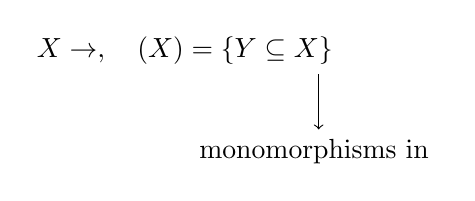
\begin{tikzpicture}[baseline=(current bounding box.center)]
    \node (A) at (0,0) {$X \to \Loc, \quad \Loc(X) = \{ Y \subseteq X \}$};
    \draw[->] (1.7,-0.3) -- (1.7,-1.0);
    \node[below] at (1.7,-1.0) {monomorphisms in $\AnStack$};
\end{tikzpicture}
\]


% 5:03
So this is a general thing you can do whenever you have a topos, or an $\infty$-topos.
It always has an underlying locale, where you only look at the monomorphisms. And if you look at the topos axioms, then you can see that unions...

\textbf{Question:} Here that possible infinite unions and intersections exist? \note{I did not hear this well}

% 5:32
\textbf{Answer:} Yes. But, I should say that potentially there are some set theoretical difficultie,s so that potentially $Loc(X)$ is not a set. I did not investigate it seriously. But in a few seconds, you will see that it doesn't matter, when I get to the definition.

\textbf{Question:} Do you mean, when you get larger and larger sizes, you could have more and more subobjects.

% 5:48
\textbf{Answer:} In principle. I didn't spend much time to prove that it is a set, because ...


\textbf{Question:} About the locale axiom, you said there is a way to produce finite binary intersection and unions, but you also have to produce infinite, I mean...

% 6:12
\textbf{Answer:} This category $\AnStack$ has all limits and colimits. We don't have to do anything special here to make this definition work.

% 6:20
\textbf{Question:} Why is the colimit a submonomorphism? Ah, you take the colimit and then you quotient by the... \note{I did not hear this well}

\textbf{Answer:} That is a general $\infty$-topos thing, for example you could take the Cech-nerve of the map and take the colimit.


\textbf{Question:} And this is in what kind of $\infty$-topos, the analytic stack?

% 6:49
\textbf{Answer:} Yes. Modulo set theoretic technicalities. So it satisfies all the same exactness as an $\infty$-topos, but it is not presentable, so...

% 7:00
\textbf{Question:}  OK, so it could be some...

% 7:10
\textbf{Answer:} So maybe $\{ Y \subseteq X \}$ is not a set, I don't care, and you'll see when I make the definition.

% 7:12
When I make the definition that I'm interested in, it doesn't matter whether it's a set or not. 

\textbf{Question:} The monomorphism, if I only consider \note{I did not hear this} that's like taking connecting component. 

\textbf{Answer:} Exactly, so it means that if you do the fiber product of  $\{ Y \subseteq X \}$, then the diagonal, I mean the diagonal map associated to this inclusion is an isomorphism.


\subsubsection{Ask for map of locales} \label{subsubsec:ask_for_map_of_locales}
% 7:40
A topological space also gives rise to a locale. But let me actually change perspectives and just say "$S$ is a locale", instead of saying "$S$ is a topological space". 
% 7:52
Then we can ask for a map of locales, $Loc(X) \to S$. Whether or not $\{ Y \subseteq X \} $ is a set, this is some data that makes honest mathematical sense. A locale is by definition the collection of open subsets, which is a set. You are saying that for every open subset, you have to give such a monomorphism, and  unions have to go to unions and finite intersections have to go to finite intersections.


% 8:26
\textbf{Question:} In the literature about locales, I don't remember, I don't use it much, but this is like the direction of map of topoi \citeme{}, but I don't know when they define M of locales \note{I did not hear this}, is it in the other direction or in this? 

\textbf{Answer:} I don't know either. So I'm doing the geometric morphism of locales. 

\textbf{Question:} Well, morphism of sites...

\textbf{Answer:} Morphism of sites goes the other direction. I'm talking about a geometric morphism. 

\textbf{Question:} But also a morphism of sites \note{I did not hear this} also goes in the other direction.

\textbf{Answer:} Maybe, I forgot.

\textbf{Question:} For locales it is not used much by algebraic geometers.

% Back to lecture
% 9:26
\subsubsection{Ask for a stronger property} \label{subsubsec:ask_for_a_stronger_property}
But we can also ask for a stronger property, so that each inclusion of open subsets, say $ U \subset V \subset S$, maps to, so it's supposed to give some monomorphisms, so maybe I should give some name for this, like $f$ or $Pi$, maybe, so $Loc(X) \xrightarrow{\pi} S$. So this: $

U \subset V \subset S \mapsto \pi^{-1} U \subset \pi^{-1} V \subset X

$. 

% 10:17
We could ask that these inclusion $\subset$ maps are actually open immersions, from the perspective of the six functor formalism that Peter discussed last time. That is, the extended six functor formalism on analytic stacks. So we could ask that each of these inclusions be shriekable, and that they be well cohomologically smooth.

But in the case of a monomorphism, then it's quite easy to see that the dualizing object is canonically the unit, and it's the same thing as an open immersion. 
% 10:56
A general monomorphism could look like anything really. It could look closed, it could look open, it could look like some mix. But it's reasonable to ask for this stronger property, that what looks like an open immersion on the level of the topological space also looks like an open immersion from the perspective of the six functor formalism.

% 11:24
\subsubsection{Metrizable, fin. dimensional CHausdorff case} \label{subsubsec:metrizable_etc_case}
In the case where $X$ is a metrizable, finite dimensional, compact Hausdorff space, we can ask for, as before, a map $X \to S$ in $\AnStack$.

% 12:00
\textbf{Question:} This is just a clarification. When you say $S$ is a locale, what is the definition of a locale? What does it mean for you for $U$, $V$ to be an open set inside $S$?
\textbf{Answer:} I'm using a bit of loose terminology here. But the definition of a locale is that it is a certain poset. That axioms that you impose on this poset are the axioms that are satisfied by the poset of open subsets of a given topolocal space.
% 12:30
But by abuse of notation, I'm using this symbol $U \subseteq S$ to mean that $U$ is an element of the poset which $S$ is secretly. But it is because I am thinking of it as a topological space \note{I didn't hear the last word}


\textbf{Question:} Equivalently suboject or the final object \note{todo} 

\textbf{Answer:} Inside some topos, yes. 

\textbf{Question:} Then this defines kind of localic reflection topos...


% 12:53
\textbf{Answer:} There is another perspective, it goes like this. You take the definition of a topos but instead of sheaves of sets you look at sheaves of truth values. I don't know if this is helpful or not.

%13:08
An usual topos would be a $1$-topos. Then a locale maybe would be a $0$-topos or something like that, I don't know.

(This is just a restatement from transcriber)
So the three situations where
\begin{enumerate}
\item Can ask for a map of locales
\item Can also ask for a stronger property, that each inclusion of opens...
\item In case $S$ metrizable, fdim, CHaus, can ask for a map $X to S$ in $\AnStack$
\end{enumerate}


%13:25
If you have this kind of structure of item 3, then you get this kind of structure of item 2. If you have this kind of structure of item 2 (topologically), you get this kind of structure  of item 1.
% 13:35
Note also that if you fix $X$ in $S$ ($Loc(X) \to S$ \note{$\pi$ above arrow}, \note{todo} they are all just sets. They are not anima or whatever, because here we just asking for a map of locales. It is just a map of posets in the other direction. 

\textbf{Question:} Note that when you say set, it also means in this sense of the set theoretical size difficulties.

% 13:56
\textbf{Answer:} That's true. So, up to size difficulties. I mean, there are no automorphisms of any fixed on of these $$Loc(X) \to S$. There are no non-trivial automorphisms. That is a good point. 

% 14:11
So 3 to 2 is tautological. Why does 3 imply 2? Basically, you can just check on the level of the analytic stack associated to such a guy that every open inclusion, actually is an open inclusion from the perspective of the six functor formalism. Peter more or less discussed this last time, that our six functor formalism on analytic stacks, when we restricted to this case, recovers the usual six functor formalism on locally compact Hausdorff spaces. And then this property of being an open immersion is stable under base change

% 14:54
\textbf{Question:} So can you say, so you know that open immersion holds for, ah, it is stable under morphisms of analytic stacks or... \note{I did not hear this}

\textbf{Answer:} It is stable under pullback.


% 15:16
Item 3 is the strongest condition. If you have item 1, you can ask whether item 2 holds. You just check whether certain inclusions or open immersions. If you have item 2, you can ask whether item3 holds. As we discussed the last couple of times, that corresponds to some connectivity condition on the idempotent algebra, as you see. 

\note{todo the following, I did not hear it well}
% 15:36 Example is started, but there is a question/remark. The example is restarted at 17m10
The second one is given off by, lo, is one of open, opener, that's true. You could think of this in terms of there's, lo, local X, and then there's some quotient local which is like the local of monomorphisms that are open versions with respect to the six functor formalism, and then the second bit of data is a map like this, thanks for that remark, Peter.

And is it the case that the union, maybe I go confus, union of open immersions is an open immersion or to make it an open, no, that's true, that it's an open immersion, which is needed to, well, it's needed to, it's needed to have this local, I mean, so, or well, remote, I mean, depends on how your, whe. No, but it's true, so that if you have a union of open immersions, then it's still an open immersion, and that's an important point to check when you're discussing these things, and it follows from this extension procedure for six functor formalisms that Peter discussed.
% 17:06
If you have a union along open immersions, then those are sheafable maps, and but it's also a cover, and you can get a a lower shriek map defined on the union and then you can actually check locally that it's cohomologically smooth.


% 17:10
\begin{example}[\yt{17m48s}{Huber pair}]

Let's give an example. Remember way back when we had Huber pairs $(R, R^{+})$ and stuff like that. Then we assign to this an analytic ring solid  solid. Then, we can take its spectrum $\Spec((R, R^{+})^\solid)$. And then we can look at the locale $\Loc(\Spec)$ associated to this.

\[
\begin{aligned}
    &(R, R^{+}) \quad \quad \text{Huber top. space of cont. valuations} \\
    &\begin{tikzpicture}
        \draw[->] (0.0,0.5) -- (0.0,-0.5);
        \draw[->] (4.5,0.5) -- (4.5,-0.5);
    \end{tikzpicture} \\
    &\Loc(\Spec((R, R^{+})^\solid)) \rightarrow \Spa(R, R^{+})
\end{aligned}
\]

 What we essentially already saw, was that this analytic stack localizes along the usual Huber topological space of continuous valuations $\Spa(R, R^{+})$.
\end{example}

% 18:14
\textbf{Question:} Now you consider the $\Spec$ in your...

\textbf{Answer:} This is what this is,  $\SpecAn$ etc. So, I'm lazy, I say $\Spec$.

\textbf{Question:} And then, $\Spa$ in the old sense.
\textbf{Answer:} Yes. 
\textbf{Question:} It's a topological space.
\textbf{Answer:} Yes. 
\textbf{Question:} And then, okay, the local, okay, and then you have a map of, \note{todo}

This $\Loc$, this means for every open in the adic space, you give a monomorphism of analytic stacks. Of course, this involves passing to some derived Huber pairs in some sense.
\textbf{Answer:} Yes. 
\textbf{Question:} Because you are not, but your original pair is not derived.

\textbf{Answer:} So on the level of rational opens, this is going to give another affine analytic stack, which is the one where you enforce that $f$ is invertible. In the world of analytic rings, you enforce that 
\begin{itemize}
\item $f$ is invertible,
\item $\frac{g_1}{f}, ..., \frac{g_n}{f}$ is solid.
\end{itemize}

% 19:45
That defines some analytic ring, under this analytic ring here, and passing to $\Spec$ it is a actually a monomorphism, on the level of the derived categories, for example, it is a localization. 
% 20:04
That gives some inclusion of analytic stacks here. 
% 20:15
We proved a less precise version of this claim early on, when we argued that the derived category...

% 20:30
So this refines the statement that $D((R, R^{+})^\solid)$ localizes on $\Spa(R, R^{+})$.
% 20:48
Recall that you have a sheaf of $\infty$-categories on this topological space $\Spa(R, R^{+})$, whose global sections is equal to this $D(R, R^{+})^\solid$, and whose sections on a rational open is the analogous category where you impose these conditions \note{todo, add latex ref to 2 conditions}

% 21:00
We had several discussions about when this is also of this form for some non-derived Huber pair and so on if you're using a Tate-Huber pair and Shifi \note{todo, didn't hear this wel} then in particular, this is just again of the same form $\Loc(\Spec(...))$ as before.
% 21:26
It refines the statement, and the proof of this statement that we gave actually shows this stronger claim. 

% 21:35
So what we did, is that we argued that you can always refine any open cover here so that, so you get an open cover. So in fact, we showed, without having introduced the language for it, that any open cover or cover of a rational open in $\Spa(R, R^{+})$, after refinement, pulls back to an open cover, under $\pi$ to an open cover, in the sense of the six functor formalism.

% 23:15
\begin{remark}
Let me make a remark. In general, it's not true that a rational open pulls back to an open immersion. 
\end{remark}

\begin{example}[\yt{23m44s}{Example of remark}]
I'll give an example right now.

% todo, correction in lecture
So, have two formal variables, $p$ and $X$. Oh, sorry, I should say $\Z_p$. I don't need two variables. Thanks. So one formal variable and then invert it. 

$ (\Z_p, \Z_p) \to (\Q_p, \Z_p)$ \label{eq:z_p_to_q_p}

What does this correspond to? 

On the level of analytic rings, we get this:

$ (\Z_p, \Z_p)^\solid \to (\Q_p, \Z_p)^\solid$

and on the level of derived categories, this is solid $\Z_p$ modules, and then this is algebraically inverting $p$. 

$ D(\Z_p, \Z_p)^\solid \to D(\Q_p, \Z_p)^\solid $ 

% 24:52, small correction
The right adjoint here is the inclusion of the full subcategory where $p: X \to X$ is invertible.

So this passing from $\Z_p$ to $\Q_p$ is algebraically inverting $p$, $p$ is a prime. 


% 25:19
And that actually, from the perspective of the six functor formalism, is a closed immersion, not an open immersion. That's a proper map, because the second variable hasn't changed, so we're changing the underlying ring and not the analytic ring structure. But it's also a proper monomorphism, it's a closed inclusion. 

% 25:42
It's a closed immersion, not open.

\textbf{Question:} So, I think we treated the case of some covering given by a function like $f$, like the Laurent cover, the one where $f$ or $1-f$ is less than or equal to mean, this kind of basic cover. And for those, is it the case? 

\label{r_is_tate}
\textbf{Answer:} Yes, so then let me make another remark. However, if $R$ is Tate, then indeed, this doesn't arise. So in general, the problem is exactly these open covers in the Huber sense, which are given by algebraically inverting a function, without enforcing any inequalities. But in the setting of a Tate-Huber pair, then you know, if you want to invert something, it's, the subset where you invert something can always be written as a union of subsets obtained by forcing inequalities.

% 26:55
\textbf{Question:} So, it is not quasi-compact in general.
\textbf{Answer:} Right. It is not going to be quasi-compact.

\textbf{Question:} But dealing with something which is in the sense of the adic space is quasi-compact, because it is a rational domain. I think in the... 

\textbf{Answer:} Yes, but...

\textbf{Question:} I mean, it is rational, so it is quasi-compact in the...

% 27:34
\textbf{Answer:} Yes. This also has to do with the fact that we didn't directly... I was sliding one little thing under the rug here, which is we didn't really directly define this \note{refer to this} as a map. We didn't really directly define it like this. Remember we actually had this valuative spectrum of all of these guys, and we actually defined this map and then we used Huber's retraction here. So this was not quite accurate, because that would be accurate on the level of $\Spv$, but that's not exactly how we get it for $\Spa$. 

\textbf{Peter:} Instead, we just assume that the real $\mathrm{Spa}_a$. \note{todo}

% 28:09
\textbf{Question:} The idea is open, and then it's okay.

So, the point is that the rational opens in the Tate case (when $R$ is Tate \ref{r_is_tate}) can always be described by forcing inequalities among the valuations. Let me try to finish what I was trying to say. I want to give an idea of what's going on, I don't want to get too precise about it, but it's this kind of phenomenon, where these guys correspond to this kind of thing, which does correspond to an open immerson \todo{add what he is pointing add}. In general this is closed and in complete generality your subsets are going to be a mix of open and closed.

% 29:15
\textbf{Question:} So, sheaves on this $F$ is not there. In fact, you cannot algebraically invert $F$, but using the right-hand side. 

\textbf{Answer:} That's right.

Also, $\exists$ another topology on the same space $\Spa(R, R^{+})$, with the same constructible subsets, where the open pulls back to open.

So, another fix, even outside the Tate case, is to choose a slightly different topology from the one Huber described, where both of these things are open \note{todo, not what he points at}. 

\textbf{Question:} It's not the constructible topology?

\textbf{Answer:} It's not the constructible topology, no. 

% 30:25
\textbf{Question:} Is it a topology which is less...

\textbf{Answer:} It is incomparable to the Huber topology. For this subset here \note{add where he points at}, $p \neq 0$, it will be closed from one perspective and open from the other perspective. It's open from Huber's perspective, but will be closed from the perspective of this other topology.

\textbf{Question:} Is it a spectral space?

\textbf{Answer:} Yes.

% 30:58
\textbf{Peter:} \note{can't hear this} Zariski closed sets should be open now, instead of closed.

Peter is saying, basically, you redeclare Zariski open subsets to be closed, 

\textbf{Question:} Which  Zariski open... They are not open.


\textbf{Answer:} For example, inverting $p$ here \ref{eq:z_p_to_q_p}. 

\textbf{Question:} Inverting $p$, is now closed in the new topology. 

\textbf{Answer:} Yes.

\textbf{Peter:} We haven't discussed so far that every algebraic inverted element ... \note{can't hear this} 
% 31:49
\textbf{Answer:} That's true, we haven't talked about that. But let's leave that aside, I think there's already enough information being discussed.

\textbf{Question:} Is it the opposite spectral space? \note{can't hear this}

\textbf{Answer:} No, it's not the opposite spectral space, because these \note{add what is being pointed at}ones are still the ones where you're enforcing inequalities like $f \leq 1$, that's still open in both cases. 

% 32:17
\textbf{Question:} It is the opposite of something Huber describes in one of his papers? He defines a lot of topology and one of them...

\textbf{Answer:} It is opposite of one of the ones Huber describes in one of his papers, yes. 

% 32:29
\textbf{Question:} we can make this more precise when ... closed \note{can't hear this}

\textbf{Answer:} I'm going to hesitantly say yes, it's obvious if you remember the definitions of everything. 

\textbf{Question:} Maybe we need \note{can't hear this} compactness or not, because you want an idempotent \note{can't hear this} to correspond to it, but I'm not sure whether if it's not quasicompact, you have...

% 33:01
\textbf{Answer:} Let me say quasicompact. It's something we've actually discussed before in the course. I drew some pictures trying to explain why it makes sense that Zariski opens should be closed. I don't know.

\textbf{Question:} All rational subsets are defined by inequalities. $f_i \leq g_n, g_n \neq 0$, 

\textbf{Answer:} Yes.

\textbf{Question:} And this one you replace by...

\textbf{Answer:} We say that is a closed condition. 

% 33:41
\textbf{Question:} For any $g$? Let's say you have a rational open, so the conditions are satisfied, like the ideal generated by all of them \todo{add what is being pointed at} is open. So, you can't invert $g$ if that doesn't correspond to a rational open in Huber's sense, but in situations where you can, it corresponds to a closed inclusion.

% 34:09
We actually discussed this topology in the notes on condensed mathematics and complex geometry \citem{todo https://people.mpim-bonn.mpg.de/scholze/Complex.pdf}. I think it was in the chapter called GAGA redux, we discussed this modification of Huber's topology. Apparently, it's also in one of Huber's papers, just passing to the opposite.

% 34:49
\begin{remark}
One last remark about this general setup: 

If $S_i$ is some inverse system of compact Hausdorff spaces, then giving compatible maps from $\Loc(X) \to S_i \forall i$ is equivalent to giving a map from $\Loc(X) \to \varprojlim S_i$. 
% 35:35
The only claim I'm making is that inverse limits in topological spaces are the same as in locales in this specific situation, which is something you can quite easily see. 
% 35:48
Also, it's the same for $\Loc^{\op}(X)$. \note{todo, add commuting diagram} If all of those ones factor through $\Loc^{\op}$, then this one will also factor through $\Loc^{\op}$.

% 36:19
There is a remark that every compact Hausdorff space is a limit of metrizable finite-dimensional spaces, (potentially in many different ways, but in many situations, there's a natural way of doing it). We'll see this in the setting of Berkovich spaces. Then this gives you a way of going from the case of metrizable finite-dimensional compact Hausdorff spaces where you can sometimes go from this perspective \note{add what is being pointed at} and you can go to this perspective, and then you're closed, the situation passes to inverse limits in a nice way, but now you no longer have to worry about things being metrizable or finite-dimensional.
\end{remark}

% 37:19
\textbf{Peter:} \note{todo}

is a map to s the same thing as a map from loal? 

% 37:32
\textbf{Answer:} No, because you have this connectivity condition. You still have to impose this locally, that locally all the itempotent algebras are connective. It's not like I produced a counter example, but I kind of believe that it's not the same.

% 38:18
\textbf{Question:} I'm always confused, is there really a t-structure def over D of that object? 

\textbf{Answer:} No, there's no t-structure. I don't have to say what I mean by connective. I have to say what I mean by connective locally. What I mean by connective locally, is that there exists a cover by affine things such that it's your object, when you pull back to each of those affine things is connective. Now, once you're in the affine world, connectivity is a pullback of something connective, you have a t-structure and the pullback of something connective is connective, so it's kind of. 

% 38:53
\textbf{Question:} And also, if the pullback is connective, then it's connective or not? 

\textbf{Answer:} No, that is not necessarily true.

\textbf{Question:} So it's not a sufficient condition for having a map. 

\textbf{Question:} So this is like for schemes, that you have the the non-affine opens, but still, if you use as the flat or pqc, still if it's affine up, it's affine down \note{not sure of this}, so that's... But in your topology, of course, you have much more stuff, 

\textbf{Answer:} Yes. So you can have these weird things where you have a map which is affine locally, but with a map with affine target which is affine locally, but not globally. That's kind of unavoidable when you're doing analytic geometry.

\begin{unfinished}{40:05}
% 40:05
\subsection{Preliminary definitions} \label{subsec:preliminary_definitions}
\subsubsection{Banach rings} \label{subsubsec:banach_rings}
So Berkovich spaces. Let me start with a reminder on the definition, so we know where we're going. $A, \norm{\cdot})$ is a Banach ring. That means that $A$ is a commutative ring, and this norm map $\norm{\cdot}: A \to \Rnonneg$ satisfies:

\begin{itemize}
\item $\norm{0} = 0$
\item triangle inequality, $\norm{x + y} \leqslant \norm{x} + \norm{y}$
\item $\norm{xy} \leqslant \norm{x} \norm{y}$ so it's sub-multiplicative
\item either $A = 0$ or $\norm{1} = \norm{-1} = 1$
\end{itemize}

% 41:01
\textbf{Question:} So, probably have to put the norm of -1 is equal to the norm of one, which is either zero...

 I should probably put that, so either a equal Z or Norm of 1 equal 1 and Norm of us one, also do you need that? It does not follow I'm not sure how much it follows, but it, it's usually they want the triangle inequality Al with $x + y$, okay. I think you can, you can get it, you can give a crazy thing like the negative multiply by two, you can do something that still satisfy the a without, but of course, it would be equivalent something satisfying the a, this is probably not how to show, okay.

Then $A$ is complete, with respect to the metric $d(x,y) = \norm{x-y}$. 

\begin{example}[\yt{42m24s}{Banach ring}]
So an example, there's, so example for, say, $S$ is a compact hausdorff space, you could take for $A$ to be, say, complex-valued continuous functions,
$A = \Cont(S; \C)$

and take the norm to be the sup norm, where you have the usual absolute value, and this, maybe this is kind of right. 
$\norm{f} = \sup_{s \in S} \norm{f(s)}$

\note{todo, last bit of eq I can't see}
\end{example}
 
\begin{example}[\yt{43m04s}{Tate-Huber ring}] 
 Another example would be if $R$ is a Tate-Huber ring, and if you choose a pseudo uniformizer, topologically nilpotent unit, then you can define a norm, Peter actually wrote down the
\end{example}

Yes, this is multiplicative. It's not multiplicative in general.

\begin{align*}
(A, \norm{\cdot}) \leadsto \BerkSpec(A, \norm{\cdot}) = \{ \norm_{x} = A \to R todo \} \\
\text{\underline{multiplicative seminorm}} \\
with \norm{f}_x todo \norm{f} \\
\forall f \in A.
\end{align*}
And then to this data, so to $(A, \norm{\cdot})$ Berkovich assigned the space, which as a set is given by the norm of $f$ equals $z$ if and only if $f$ equals $z$, right.
% 46:30
So, I'm using this notation $X$, so kind of it's a decoration to. And this is now a \underline{multiplicative seminorm}, with which is bounded by the given norm you have on the Banach algebra $A$.

\begin{example}[\yt{47m13s}{Tate-Huber ring}] 
\begin{align*}
A = \Cont(S, \C) \\
\norm{f}_x = \norm{f(x)} \forall x \in S.
\end{align*}
Well, for example, in and you can take. If you require that the norm restricts to the usual Norm on the complex numbers, then these are all the examples. So that's Gelfand's theorem. So, those are the only examples in this situation. And multiplicative includes the zero element, that is $\norm{1} = 1$, yes.

Except, but this is maybe zero multiplication of zero numbers, we don't want that. So, we want these to be like points, so we want them to be non-empty. So, we want one to be different from zero.

But, do you allow $\Z_R$? No, well, wait, I allow, okay, I allow $\mathbb{A}$ is the zero ring, when this will be the empty set.
% todo, move this end example
\end{example}

\begin{align}
\BerkSpec(A, \norm{\cdot}) \subseteq \prod_{f \in A} [0, \norm{f} ]
\end{align}
This is actually a compact Hausdorff space. I didn't describe the topology, but here it is. You can view it as a subset of the product over all $F$ in $A$ of the interval from zero to the norm of $F$. It is actually a closed subset. This map takes a norm and records its value on $F$. The topology is the subspace topology, so it is a compact Hausdorff space.

\subsection{Berkovich spaces in the language of analytic stacks} \label{subsec:berk_spaces_language_analytic_stacks}
% 50:20
So what we're going to do is, we're going to try to make the same definition, but in the world of analytic stacks instead of topological spaces. So, we want to take the same idea, which is that we want to look at the set of all multiplicative seminorms $\BerkSpec$ on $A$, bounded by the given norm on $A$, but we want to say that in the language of analytic stacks, using the notion of norm on an analytic ring that we discussed earlier.

\subsubsection{Norm} \label{subsubsec:norm_reminder}
% 51:18
Let me remind you about this notion of a norm. So, the definition of, we could say even more generally in an $\infty$-category stack. 

% TODO: when the earlier lectures are transcribed, we can see what we need to copy here.

A \emph{norm} on $X$ is a map $\P^1_X \xrightarrow{N} [0, \infty]$, including $\infty$, which is multiplicative (so away from $\infty$, so, let's say on $N^{-1} ([0, \infty))$ and let me write it suggestively like this: $N(T^{-1}) = N(T)^{-1}$. $T$ is the variable on $\P^1$. You really should write down the commutative diagram with inversion on $\P^1$, inversion of the coordinate on $\P^1$ and inversion of this extended real positive non-negative real axis here. 
% 52:34
And some condition on how $P$ sits.

\textbf{Question:} What do you mean by how $P$ sits?
% 53:19
\textbf{Answer:} So, remember $P$ was this ring object you have over any analytic ring, which is the free guy on a topologically nilpotent element. And it's some version of a unit disc, and what we ask is that this Norm function gives you another version of the unit disc, which is like the inverse image of the closed interval $[0, 1]$ or you also have the inverse image of the halfopen interval from , and you want to say that $P$ sits in between the two of those.

% 54:00
Write $\mathcal{N}(X)$ for the set of norms on $X$. So recall $\mathcal{N}$ is an analytic stack. (It is a set. It is just given by a map in our category and our category is locally small.)

% 54:38
A map in the category of analytic stacks. So these objects are fixed, right? When you fix $X$, this is fixed, and this is fixed. 

\textbf{Question:} Yes, that you know that there is a. Why was it? 

\textbf{Answer:} Well, basically by definition, every analytic stack was a small colimit of representable analytic stacks. You have a.

% 55:28
\textbf{Question:} Because there was a notion of analytic ring where there is the category. Okay, there, you handle the problem of large sizes. I mean, because it's enough to check the condition on some small... But then you have the notion of analytic stack where you cover, but you don't know which covering you need to give a morphism, so you have need all possible covers, could be covers by bigger and bigger see, but you say the category is accessible. 

% 56:01
\textbf{Answer:}
So the main technical result you need to prove is that the sheafification of an accessible presheaf is still an accessible presheaf. That's the main technical result you need to prove. We did not discuss this at all, but that's what's underlying the resolution to these issues. It's like in Waterhouse.

% 56:35 todo, notation
In fact, $\exists$ a cover, so $\Spec(\Z[q]\gas) \to \mathcal{N}$. In other words, you can write down a norm on this gaseous space stack, and this is actually the universal norm on an analytic ring (R^\tri, D(R))with a variable $q \in R^\tri \st  N(q) = \{ \frac{1}{2} \}$. 


\textbf{Question:} What did you write? $\mathcal{N}(X)$ is the analytic stack

% 57:43
\textbf{Answer:} $\mathcal{N}$ is an analytic stack. So $\mathcal{N}(X)$, the set of norms, is actually the set of maps from $X$ to some stack $\mathcal{N}$.

So if you ask for a norm on an analytic ring and an element whose norm is exactly equal to $\frac{1}{2}$, which is kind of a somewhat stringent condition, because a priori again, the norm map $N(q)$ is a map $\Spec(R) \to [0, \infty)$, and you're asking that it factor through this \note{I don't understand this phrasing}, a priori, its image could be some interval or something, but you're asking that its image be exactly this singleton. The universal example of that is this guy $\Spec(\Z)$ \note{todo, notation}, and moreover, the map to the base stack is actually a cover, in the sense of our Grothendieck topology on analytic stacks, because every norm on an analytic ring locally, you can find such an element. We had this argument, we discussed this two lectures ago. 

% 58:45
\textbf{Question:} Everything here was like $X$ was a $\Spec$ of an analytic ring. 

\textbf{Answer:} I made this definition for a general $X$, but it doesn't matter, because the condition, the norms on an analytic ring, they satisfy descent basically. I mean, it's kind of follows from general nonsense, and so it automatically glues to say what a norm is on an arbitrary analytic stack. It just unwinds to the same thing. 

\textbf{Question:} So the cover also exists because it exists locally, like you GRE it. 

\textbf{Answer:} Well, the map, the map, no, the map exists because you can write down this norm, and then it's a cover because given any norm on an analytic ring, after a cover, you can find a $q$ that satisfies this property.


% 1:00:20
\subsubsection{What does $\mathcal{N}$ look like?} \label{subsubsec:what_does_n_look_like}

Before finishing the introduction of the definition of this enhanced Berkovich spectrum as an analytic stack, I want to explore a little bit about what does $\mathcal{N}$ look like? So, what do we have on $\mathcal{N}$ if you have a norm on an arbitrary analytic ring? So, if you have a norm $N: \P_R^1 \to [0, \infty)$, so as mentioned, for any section here, you get a function from $\Spec(R) \to [0, \infty]$, but over an arbitrary analytic ring, the only thing we know exist are the integers. 
% 1:01:42
So, given $n \in \Z$, we get a map which records the value of your norm on the integer $n$. So, what does this
We'll also see that the fiber over any point in the image is non-empty, so that at least in this case, maybe it's a general fact - I don't know, at least in this case, it's kind of a theorem that the image is closed, so to speak. Now note that the more traditional thing is this Berkovich spectrum of the integers, that was also by definition a subset of this product going from $\prod_{n \in R} [0, \infty]$, and it was given by those norms, so multiplicative, avoiding Infinity, satisfying the triangle inequality.

% 1:02:30
So we want to know what the "image" is, so to speak. Let me say what I mean by image. I mean the \emph{complement of the largest open subset $U \subset \product[0,\infty] with \pi^-1 U = \empty$}.

Let me remind you what this thing looks like, in case people haven't seen this before. Recall that $\M(\Z)$ looks as follows: you have a point at the center, so to speak, which corresponds to the trivial norm, meaning the zero norm of $Z$ is $Z Norm$, and the norm of everything else is equal to one. 
% 1:05:33
Then, you have several branches. You have an archimedian branch, so at the end of the archimedian branch, you have the usual norm, the usual archimedian norm, the usual absolute value. But then, for each prime $p$, you have another branch, which also ends at some point. To get the correct topology on embedding it into $\R^2$, you should probably make the branches get shorter and shorter and shorter, but okay, that's...
% 1:06:10
But the situation with these $p$-adic branches is a little bit different. So, what's going on here? Here, you have the usual absolute value, and here, at the halfway point, you have the square root of the usual absolute value. And here, you can then you can put any $\alpha$ between zero and one, and you can kind of see from the intuitive perspective that this interpolates between the usual absolute value and the trivial absolute value. 
% 1:06:34
Here, what goes at the top is not the usual $p$-adic absolute value; the usual $p$-adic absolute value sits somewhere here, so normalized to say so that P equals 1 over p. And now, you can actually scale it to $R_{>0}$, and then there's also a limit as the scaling goes to infinity, and what that gives is the trivial norm or the pullback of the trivial norm on the residue field $FP$, so in other words, the norm of any multiple of $p$ is equal to zero, and the norm of everything else is one.

Okay, what of course, no, I... This is great. I think this was something like this, this is the first talk. There was a talk in this course, it was in this course or another, probably in this course, there was some discussion of, but maybe I could do this another thing. 
% 1:07:42
So I'm trying to recall something which is well-known indeed, in order to set up the discussion of what's following here. So, in particular, I want to emphasize this is a really big space, but the subspace $MZ$ \note{todo} is quite small, you know, one-dimensional.

\textbf{Question:} So, now what we're going to see, so there, you allow the value to be in, but here, you don't. 

% 1:08:13
\textbf{Answer:} That's correct. So, here's going to be the claim: the image of the norm $\text{Im}(\mathcal{N})$ is a larger subset. It looks like this: you have all the same ones as before, sorry, I'm trying to say that it stops there, trying to draw like a closed interval sign, but then also at the archimedian place, it gets extended. So, here now the usual archimedian absolute value is also in the middle of the interval, and you can take arbitrary powers of it, so for any $\alpha \in R_{>0}$, you can take powers of it. So, it'll go to there in one direction, and to the other direction, you get some really strange point, which corresponds to... 
% 1:09:23
So, it's a subset of there, so it's given by some maps from $\Z$ to the extended real line there, and it's given by $N(n) = \infty$ if $n \neq -1, 0, 1$.

% 1:10:17
\textbf{Question:} \note{todo}
\textbf{Answer:} No, it is a different kind of base. Because over Solid $\Z$, $\R = 0$ you can't.

\textbf{Question:} \note{todo}
% 1:11:18
\textbf{Answer:} It extends to to infinity and then compactified at the end. You can try to write a formula for it. It's like the image norm is like - you take the Berkovich space of the integers. Ah, no, let me make a before I say this.

% 1:11:35
In particular, the triangle inequality can fail. That's quite clear here - you have $N(1) = 1$, but $N(2) = \infty$. That's a pretty drastic failure of the triangle inequality. But also, like for the square of the usual absolute value, which is a new thing, you have the triangle inequality fails as well.

% 1:12:05
So, another way of saying this is $\text{Im}(\mathcal(N)) = \BerkSpec(\Z)$ - you can get it from the Berkovich spectrum of $\Z$. On the Berkovich spectrum of $\Z$, you have an action of the real numbers greater than or equal to one. Wait, did I - or well. Or maybe, on this other thing, you have an action of the positive real numbers. You can do this, and that doesn't do anything on the non-Archimedean branches, and then on the Archimedean branch, it extends it all the way, and then you compactify it - one-point compactification. So, I don't know.

Let's explore this and let's see what is going on. Let's consider the map - what's that? Is the one-point.

\textbf{Question:} The picture you seem to see this image gen topological space, but this is supposed to be something associated with $\Z$, right? That's a good question. So, by definition, I made it a - I was saying it's a closed subset of the topological space. Now, you can view this as an analytic stack. We saw how to view this as an analytic stack, and you can take the product in the category of analytic stacks - that's perfectly legitimate. It's no longer finite dimensional - sorry, it is metrizable, it's no longer finite dimensional. So, we didn't quite talk about this thing, but you can still view this as an analytic stack, and you still do get a map of analytic stacks from $N$ to this product, and this closed subset does correspond to a subanalytic monomorphism of analytic stacks here, and the map from N there does factor through that closed subset, and so you can view it in several different ways.

% 1:13:00
Okay, to explore this, consider a fixed prime $p$, and consider the norm of $p$ 
$
\mathcal{N} \xrightarrow{N(p)} [0, +\infty]
$
. 
% 1:15:15
Here's the first claim: we can understand the locus in this universal space of norms where the norm of $p$ lives in $[0, +\infty]$. This is the same thing as the stack parametrizing norms on which the variable $p$ lives between 0 and 1 - let's call this $N$ and $\Z$ less than absolute value of p less than one. This is equal to $\Spec \Q_p^{\gas}$, the gaseous version of the $p$-adic numbers, across this stack associated to the open interval $(0, 1)$.

Claim
$N(p)^-1 ((0,1)) = $\Spec \Q_p^{\gas} \times (0,1)$ 

% vertical equal sign
$\mathcal{N}_{0 < \abs{p} <1}$

This is quite easy to see, because we know that the universal analytic stack equipped with some variable whose norm is between zero and one \mathcal{N}_{0 < \abs{p} <1}$ is $\Spec(\Z_q)$ hat plus or minus one Gaseous cross 0,1. And then you have to impose that that variable becomes $p$, so you set $q = p$ or you mod out by $q - p$, and then that, as Peter discussed when discussing this gaseous base stack, gives you some analytic ring structure on the $p$-adic numbers, and then the second variable doesn't really change.

% 1:17:40
I'm claiming in particular that if you look at the universal - let's say we take the fiber over a point $ \lambda \in (0,1)$, 


$
Spec(Q_p^\gas) \times \{ \lambda \}      \text{normed analytic ring structure \\ here: notion of overconvergent functions on a disc of radius $r$ }
$

then you get a normed analytic ring structure here. And it is - so what does that mean? It means that for every radius $r$, you have some notion of overconvergent functions on a disc of radius $r$, where the notion of on a disc of radius $r$ is the usual one from non-Archimedean geometry, where you take the normalization of the absolute value on the $p$-adic numbers for which $\abs{p} = \lambda$. So, what we're seeing here is the interior of the $p$-branch.
Kind of fairly straightforward to understand. 

% 1:19:54
Next, let's look at another locus that's fairly easy to understand. This is the locus where $p$ is between one and infinity. 
\begin{align*}
$\mathcal{N}_{1 < \abs{p} < \infty} = \Spec(\R^\gas) \times [0,1]$

% todo arrow between above and under

$ 0 < \abs{\frac{1}{p}} < 1 $

\end{align*}
% 1:20:10
Strictly between one and infinity, because that's the same thing as saying that $p$ has to be invertible. The absolute value of $p$ is away from zero. 
% 1:20:20
Then it's the same thing as saying that the absolute value of $\frac{1}{p}$ is between $0$ and $1$. 

% 1:20:27
We can again use the exact same argument to understand what this is, and what you get is you get $\Spec(\R^\gas) \times [0,1]$, and the argument is the same. As Peter explained, if you take this ring and mod out by setting $q = \frac{1}{p}$, then you actually get the real numbers. You get a certain analytic ring structure on the real numbers, which is this one here \note{todo: clarify}

% 1:21:07
Again, if you look at the universal norm with a fixed value of $\lambda$, the universal norm here is the usual one given by convergent functions in Archimedean geometry, say complex geometry, but with respect to the norm, which is a power of the usual absolute value, where $\alpha$ is such that the norm of $\frac{1}{p}$ exactly gets $\lambda$.

% todo: point arrow up 
$\Spec(\R^\gas) \times { \lambda }$

% 1:22:10
\textbf{Question:} I'm not quite sure where the overconvergent functions show up. You had some formal series in this $q$ \note{not sure}, but then you specified that it is the usual overconvergent functions. The first thing to understand, of course, is why when you take this ring and specialize to $q = \frac{1}{p}$, you get the real numbers. That has to do with some kind of base-$p$ expansions. \note{need to go over tis question again}

% 1:23:04 todo, clarify which expression he points at
\textbf{Answer:} You have to do a calculation. The first thing to understand is why if you take this ring and specialize to $q = \frac{1}{p}$, why you get $\R$. That has to do with base $p$ expansions. Then you have to understand, say, if you take this module $p$, the basic module $p$, you want to know what that base change is too. It should be some module over $\R$, so it should be some sequence space with summability condition. 
% 1:23:38
You can see that the summability condition is basically some exponential decay, as Peter described.

The point is that this thing does sit between the usual ring of overconvergent functions on the unit disc and the ring of holomorphic functions on the interior of the unit disc. When you do this overconvergent business, the subtlety of exactly what ring it is and what summability property you have doesn't matter anymore. It returns the usual ring of over-convergent holomorphic functions on the disc. There some scaling of the usual absolute value, because when we were building the universal norm, we had to take a fixed value of the norm of $q$ and kind of use that to write the answer. 
% 1:24:48
It is such that if you specialize to the usual situation, you get the normal thing.

% 1:25:19
In particular: this locus $\mathcal{N}_{1 < \abs{p} < \infty} $ is independent of $p$, because the universal norm didn't really depend on $p$ \note{todo: the second part of this sentence is wrong}. There's some rescaling property of the norm, but it doesn't affect this subspace $\mathcal{N}_{1 < \abs{p} < \infty} $ of the universal space of norms. This is the kind of thing you need to see in order to see that you're getting the Berkovich space. You have some infinite-dimensional space, but the conditions on the various prime numbers are very tightly related to each other. This is like in Ostrowski's classification of norms on the integers.
% 1:26:07
If you have a norm on the integers for which the norm of $p = \frac{1}{2}$, then it has to be the $p$-adic norm. In particular, its values on all the other integers have to be determined by that. You can see that also in our situation as well. When you force yourself to live in this locus of \note{todo: 1:26:26} which is only a condition on $p$ that automatically tells you what the norm of everything else is, because you can just do calculations with these usual rings of overconvergent holomorphic in usual non-archimedean geometry. So the norm of all others is determined.

\begin{align*)
$\mathcal{N}(\text{all other n})$ is determined
\end{align*}

% 1:26:47
\textbf{Question:} So The Berkovich \note{I did not hear this }, instead of norms on $\Z$...

\textbf{Answer:} Yes, not up to equivalence. No.

% 1:27:10
\textbf{Question:} \note{I did not hear this question well}

\textbf{Answer:} Why that would be? Is there some explanation why that would be. For me, it's just a calculation. I mean, in our axioms for normed analytic ring, we had no version of the triangle inequality whatsoever. We just had this that the norm should be multiplicative. But then you can look and see, if you believe what I'm claiming, then kind of almost all of this does satisfy the triangle inequality, because you can check on in terms of the rings of functions that are being assigned, and you can verify that the triangle inequality holds. So whenever you're in the ordinary Berkovich space of $\Z$, your norm actually satisfy the triangle inequality. And then you get some sort of quasi-norm, if you move out in this direction, and this part is a little funny, but if you throw that away. 
% 1:28:08
So there's always some version of the triangle inequality that is automatically satisfied, just as a consequence of multiplicativity, and that's kind of funny.

% 1:28:15
\textbf{Question:} In the usual theory of Berkovich, in fact, was consider earlier, then I mean, it's I'm speaking now about Ostrowski's classification, so you can put the following condition. I don't remember which reference, instead of triangle inequality, you can put like $x +/- y$ val less equal to some constant times x y, and then one can prove that after a normalization by some power, you have the triangle inequality or even the.

And so is it the case that, here, you can relate it somehow where, in the locus where, so if you know that the priority that the nor some integer like or three not infinity, then you can get the triangle inequality by scaling it.

\textbf{Answer:} Yes, exactly. 

\textbf{Question:} So if, well, I have on everything now, I'm speaking about \note{I did not hear this}

% 1:29:18
\textbf{Answer:} Let me make some further claims.
Claims
\begin{itemize}
\item Claim: if you have a normed analytic ring $(R, N), N(2) \leq 1$ with 2 say, doesn't matter, less than or equal to 1, automatically satisfies the non-Archimedean triangle inequality.
\item A normed analytic ring with norm of 2 less than or equal to 2 satisfies the usual triangle inequality.
\end{itemize}

\textbf{Question:} no of 2 two is equivalent to no of 3 three, 
 
% 1:30:28
\textbf{Answer:} Yes. 2 is an arbitrary prime number here, 

\textbf{Question:} about to 6, is it

\textbf{Answer:} That's also equivalent. So I guess prime is not so important, 3 is an arbitrary integer bigger than 1.

% 1:31:08
Okay, then. 
Claims
\begin{itemize}
\item 
\end{itemize}
So a normed analytic ring with $N(2) < \infty$, there always exists a constant $ \exists c > 0$, such that $\norm(x + y) \leq C (\norm{x + y})$ is less than or equal to C * the norm of $X$, the norm of $Y$, 
\textbf{Question:} but this is interpreted not in the sense of normal functions, but it's not. 
% 1:31:39
\textbf{Answer:} It's some universal thing, like, you know, you write down, you have whatever you have, you have $\P^1$, like, the locus where the norm of the T variable is less than or equal to a, cross P1, you know, locus for the S variable is less than or equal to B, that this maps to, so it's a and b are less than infinity here, so it's this maps to P1 R, and then this maps to Z Infinity, but this should factor through zero, and then C * a plus b.

% Draw commutative diagram
\begin{align*)
$A, B < \infty \P_{\abs{T} \leq A}^1 \times \P_{\abs{S} \leq B}^1$
\end{align*}

So, and this is addition A1, they, 
% 1:32:33
it's well defined because this happens to live inside $A1$ \note{todo, check this}, which we already argued earlier.

So there's always some version of the triangle inequality.

How do you prove these claims? 

% 1:33:06
By the way, these claims imply the claim about what the image of n is, because, so, and then this extended Berkovich space, the one I mean the specific one that I wrote down, the reason is that you can, you can look at $N(2)$, which goes to zero infinity, if you want to, if you want to know the image of something, you can actually work, you can actually work on stratifications of your topologic, you don't have to work in closed covers or open covers, you don't have to work locally
Over the locus where $2$ is less than or equal to $1$, the locus where $1$ is less than $2$ is less than infinity, and then the locus where $\norm{2} = \infty$. 
% 1:34:46
We then have to take the union of the images we see there. And here, if you believe this claim, then there you have the non-archimedean triangle inequality. So, here it's automatically a subset of by some universal argument, the non-archimedean Berkovich spectrum of $\Z$. We're contained in the claimed locus there. 
% 1:35:16
This thing $1 < norm{2} < \infty$ we already classified, is contained in the archimedean locus, the archimedean locus. So, the last thing we need to do is to see that this locus $\norm{2} = \infty$ consists of one point.
Need: $\norm{2} = \infty \Rightarrow \norm{n} = \infity \forall n \neq 0, 1, -1$ 

We need for all $n$ different from $0$, $1$, and $-1$. And that actually doesn't follow from the claims well. well, the claim that these conditions are independent of $2$ does give this as well. The last thing you say plus be, that's true. You can also directly argue that if $3$, for example, wasn't sent to infinity, then you'd be in one of these loci, and then $2$ wouldn't be equal to infinity.

To prove these kinds of claims, you calculate. For the first part, we only know it's not larger than once, and it's not implied directly. Then you also need to see that if you take any point and then take that, there exists some normed analytic ring which has those values. We already saw it for the points in the interior of the rays in the Berkovich space, and it's also quite easy to hit the center because you do some non-archimedean geometry over some Laurent series ring with $\Q$ with the trivial norm, or you can hit the points at the end by doing some non-archimedean geometry with $\F_p$. This gives the containment, but you can actually see the other inclusion by exhibiting.

To prove, we can assume we have this $\Q$ with a norm of $\Q$ between $0$ and $1$, and then we're working over this Gauss to base. For the first claim here, the non-archimedean claim, what do we need to do? Well, then the universal case, given that we fix this data, we're asking that the norm of $2$ is less than or equal to $1$, so it lives over an idempotent algebra. This was because of the claim that you have a cover. You can check things like the non-archimedean triangle inequality after passing to the total space of a cover.

This idempotent algebra is the ring of holomorphic functions, so to speak, the overconvergent version of the unit disc, and then you mod out by $T - 2$. This gives a power series or Laurent series with integer coefficients that converge to radius zero, which are converge on some unspecified open disc around the origin. This already shows that the condition is independent of $2$, and then you can look at the universal over this and check the non-archimedean triangle inequality.

The only other locus you need to worry about is the locus where you're...
Between one and two, and then you're in this non-archimedean branch, and we saw you get the usual thing: you have the triangle inequality there. And then, to prove this claim, it's actually enough to - I think it's easier to prove the root. The root is, it's easiest to prove this claim, and then that implies the claim, because this means that the only other possible point to consider, we're living in the Archimedean locus, so we're some rescaling of the usual absolute value. And then, this weak triangle inequality, this quasi-norm triangle inequality, is actually satisfied.

To prove this, you again do a calculation. It's sort of similar, except you're setting $t$ equal to 2, or you're setting the inverse of $t$ equal to some weird version of functions convergent on the open disc. And again, you observe that it's independent of 2.

In this locus, your convergence property is shrinking down to zero. In this locus, the locus relevant to this claim, it's kind of the Laurent tails that are forcing the convergence out to the boundary of the unit disc.

% 1:44:07
As mentioned, there's no course this Friday, but please come here, and Peter will be here in person, and so will three other people giving talks, some of which are relevant to the material here. Next week, I'll continue this discussion of Berkovich geometry next Wednesday, and then the next Friday is actually going to be the last class, so we're really almost done here.

Regarding the question about the ontic stack sitting over the classical regions, and what it means if it sits over infinitely many points, it's a bit weird. The norm is quite different - it's an analytic norm, not the norm on a ring. This relates to the statement about the set of norms being like the rescaling of the norms and forming a stack, where any analytic space has a unique map to this stack.
According to the website, we have two more weeks. However, we may have to change that because there was some... Apparently, on the IHS website, it says we have two more weeks. But I'll get it fixed because the number of talks was originally more than the actual...

We did decide that next week is the last week, right Peter?

Yes.

What's that IASS?

Here, I see. In BOND classes, officially end, that's why we're stopping.

\end{unfinished}
% !TeX root = ../AnalyticStacks.tex

\section{\ufs Berkovich spaces II (Clausen)}

\url{https://www.youtube.com/watch?v=vXZC3WzKZgo&list=PLx5f8IelFRgGmu6gmL-Kf_Rl_6Mm7juZO}
\renewcommand{\yt}[2]{\href{https://www.youtube.com/watch?v=vXZC3WzKZgo&list=PLx5f8IelFRgGmu6gmL-Kf_Rl_6Mm7juZO&t=#1}{#2}}
\vspace{1em}

\begin{unfinished}{0:00}
This lecture is about Berkovich spaces, which is a topic I began discussing last time.

Let me remind you of the classical setup. You have a Banach ring $(R, \norm{\cdot})$, which is a ring $R$ equipped with a norm $\norm{\cdot}$ that is submultiplicative and satisfies the triangle inequality. $\norm{1} = 1$, unless $R = 0$. And $R$ is complete.

\begin{itemize}
\item $\norm{xy} \leqslant \norm{x} \norm{y}$ so it's sub-multiplicative
\item triangle inequality, $\norm{x + y} \leqslant \norm{x} + \norm{y}$
\item $\norm{1} = 1$ unless $R = 0$
\item $R$ is complete w.r.t. $\norm{\cdot}: A \to \Rnonneg$
\item $\norm{-x} = \norm{x}$
\end{itemize}

%todo insert earlier Banach ring latex def here.

% 1:45
To this $(R, \norm{\cdot})$, Berkovich assigns a compact Hausdorff space, $\BerkSpec(R, \norm{\cdot}) \subseteq \prod_{f \in R} [ 0, \norm{f} ]$, which is a subset over the product over all elements in $R$ of the closed interval $[0, \norm{f}]$. A point in this space is denoted as $x$, but what it really is, it is an evaluation map $\norm{\cdot}_{x}= R \to \Rnonneg$, which is now multiplicative ( $\norm{fg}_x  = \norm{f}_x \norm{g}_x) and satisfies the triangle inequality $\norm{f + g}_x \leq \norm{f} + \norm{g}$, with $\norm{1}_x = 1$.

% 2:43
Now it is strictly multiplicative.

\begin{remark}
% 2:49
$R$ is not complete with respect to this $\norm{\cdot}_x$. In fact, there could be many elements of norm 0. However, if you complete $R$ with respect to any $\norm{\cdot}_x$, you get a complete valued field $\mathcal{K}(X)^{\text{hat}}$, which is sort of the residue field in the sense of Berkovich theory.
% TODO: Latex notation of K residue field
Recall that there are basically three cases:
\begin{enumerate}
\item archimedian $\iff$ $(\R, \norm{\cdot}^{\alpha})$ or $(\C, \norm{\cdot}^{\alpha)$, $\alpha \in [0, 1]$ by Ostrowski
\item non-archimedian but discrete, then you have the trivial norm $\norm{\cdot}_0 = \text{trivial norm}$
\item non-archimedian non-discrete, $\norm{\cdot}_{normalize}^{\alpha}, \alpha \in (0, \infty)$
\end{enumerate}
In the archimedian case, there is no real variety in complete normed fields, as it is either $\R$ or $\C$. In the non-archimedian discrete case,. In the non-archimedian non-discrete case, the value could come from a discrete valuation, and there is an ambiguity in the normalization.
\end{remark}

% Some text about the discussion seems to be missing here
% 5:05
\textbf{Question:} Of course, on non-discrete, there is ambiguity. It's not about discrete... \note{todo}

\textbf{Answer:} Exactly, that was the parenthetical comment I was making. A non-discrete topology. Non-discrete exactness \note{todo}

% 5:31
\textbf{Question:} It is not what most people call non-archimedean. 

\textbf{Answer:} The norm is non-archimedean, but the field is discrete. It is just a discrete field.

% 5:45
So these are the three kinds of cases of possible residue field behaviors.

% 6:05
\textbf{Question:} There is no normalization.

\textbf{Answer:} No. You could choose a normalization, if you fix a pseudouniformizer and a real number, you can choose a normalization. 

% 6:29
So these are kinds of points.

% 6:36
\subsection{Promote $\BerkSpec(R, \norm{\cdot})$ to stack}
Now, the goal is to promote $\BerkSpec(R, \norm{\cdot})$ to an analytic stack, using the stack of norms, $\mathcal{N}$. A map from an analytic stack $X \to \mathcal{N}$ is the same as a certain map from $\P^1_X  \xrightarrow{N} [0, +\infty]$, satisfying norm axioms, the most important one multiplicativity, which you have to phrase a bit carefully, but in the end, it's just multiplicativity.

% 7:50
Last time, we investigated the geometry of $\mathcal{N}$, and saw that $\mathcal{N}$ lies over $\ExtBerkSpec(\Z)$, the extended Berkovich spectrum of $\Z$. The usual triangle inequality is what made the difference, the reason you couldn't take an arbitary power $\alpha$ here. If you take an arbitrary power $\alpha$, that basically behaves like a norm, but it is really just a quasi-norm. So you have to put some constants in front of here.

\textbf{Question:} Plus, you have also the kind of the limit at, 
% 8:42
\textbf{Answer:} Yes, there's also the limit at $\infty$. 
% 8:50
In this stack of norms, there's no triangle inequality imposed. It turns out that what you get, is this non-strict triangle inequality, where all powers of the usual archimedean norm are allowed. Also, there's a some kind of very strange limit point where your norm takes infinite values on natural numbers.
% 9:12
Then you have the archimedean ones, so $2$-adic absolute values which end here in a point which has both characteristic $0$ and characteristic $p$ Behavior, but where the norm of two equals zero and then for the other primes $p$.

% todo, make drawing
9:34
We also kind of saw what on the interior of these line segments, you were getting the the gaseous $\R$ theory $\R^{\gas}}, on the interior here you're getting the gaseous 2-adic numbers, and then as you move along the normed, the norm is changing, but the analytic ring is not. In $\Q_3$ and so on, and then here you have things living, you have $\F_2$ living for example, you have things living in characteristic 2 there, living in characteristic 3 here, and here you have things living in characteristic 0.

% 10:09
In some sense, you can imagine that the points of this stack correspond to something like these complete valued fields, or the minimal choices of complete valued fields like you have $\R$, $\Q_p$, you have discrete $\F_p$, you have discrete $\Q$.

% 10:32
So, that's kind of a substitute for the notion of multiplicative valuation, but then we still have to input our Banach ring $R$ into the construction in order to get something non-trivial. Here's the definition, and I don't know what good notation is, I'll write it like this.

% Definition
% todo macro for 'Nu', stack of norms?
$\Spec^\Berk (R, \norm{\cdot}) \subseteq \Nu \cross \Spec(R, \text{triv})$ 

This will be an analytic stack, which will be a substack subset of stack of norms cross, and then some affine analytic stack which is just we take $R$ with the trivial analytic ring structure. What I mean by this, is that you take an $R$, $R$ is a Banach ring, so it has a topology, but you can also view it as a light condensed ring. 

\textbf{Question:} So using the topology, you consider those condensed set?
\textbf{Answer:} Yes.

And then trivial analytic ring structure.

\textbf{Question:} that is, all modules are allowed?
% 11:41
\textbf{Answer:} Yes.

% 11:51
It's the full condensed derived category of this condensed ring.
% 11:57
So that means that if you want a map $X \to \Spec(R, \text{triv})$ that is exactly the same thing as giving a map of condensed rings from $R$ to the value of the structure sheaf on $X$: $R \to \O(X).

% 12:13
This is going to be a subset of this product consisting of those so such
so these are going by definition in bijection with so 
it's going to be a pair consisting of a norm and then a map from $R$ 
such that
and then we impose a condition 
% 12:50
I forgot to say the thing that ties this to that 
You require the multiplicative valuation to be bounded by the given norm. 
$\norm{f}_x \leq \norm{f} $
% 13:03
And that's exactly what we're going to do here.

% 13:05
such that $\forall f \in R$, 
so when you have the norm here and you have an element in $\O(X)$, you get a section of $

then you can compose with the norm and you get a map $N(f): X \to [0, \infty]$
so that this map lands inside
$[0, \norm{f

% 14:44
The first theorem would be that this is an analytic stack which localizes along the Berkovich spectrum $\BerkSpec(R, \norm{\cdot}$ in the sense that I discussed in the last lecture so that if you look at this locale of all open substacks of this $\Loc^{\op}(\SpecBerk(R, \norm{\cdot})) \to \BerkSpec(R, \norm{\cdot})$.
This maps naturally to 
this compact Hausdorff space which is the Berkovich spectrum

% 15:33
\textbf{Question:} So you have the locale of opens in the usual topology and the locale...

\textbf{Answer:} With the usual topology, oh, on the right

\textbf{Question:} But on the left, open substack means what, it means monomorphism

% 15:48
\textbf{Answer:} It means a monomorphism which is shriekable a cohomologically smooth. 

% 16:00
\textbf{Question:} This was discussed in one of the talks, okay.

% 16:06
\textbf{Question:} You could even ask for a map of analytic stacks, right? \note{not sure of this}

\textbf{Answer:} Well, when this is finite dimensional and metrizable, yes, which is basically all cases. But I mean 

% 16:31
So again, in the case when this is metrizable and finite dimensional, to verify that you have map... It really just is a condition to say that you get a map of analytic stacks to that thing and it's just you have to check some connectivity properties of these idempotent algebras assigned to closed subsets that are kind of implicit in this map.

% 16:52
So it's a condition that you can check in practice, and so is it the case that you have. Since $R$ is cool, you can think of it as a limit of C sub Rings, which are account many elements. Yes, so you can probably reduce to, no, but it maybe, it's not dimension. Well, I'm not sure, but no, no, but you can look at as a colimit over finally generated sub rings, and then, and that's always embedded in a finite I mean.


% 17:19
Okay, 

\textbf{Answer:} yes, so that's one way. So, there is indeed a canonical way to write this as an inverse limit of finite dimensional metrizable spaces, but let's not do it. Let's just work with this setup here. 


\textbf{Question:} And is it true that you have inverse limits in analytic stacks? Yes, you have, you have all limits in analytic stacks. So you can syn of it as a limit over the stack, is a limit over the, well, this isn't a stack now. I'm just viewing this as, when you have those nice things, you can construct.

Okay, so it's not, no, but then you can take for the nice subing, you can take the stock Associated to m in those limit, you get something which is, yes, you get something. 


\textbf{Answer:} Then you get something, the only problem I have with that, it's not a real problem, but just is that if you started with something which happened to be already be finite dimensional and metrizable, then you'd be non-trivially writing it as an inverse limit of other finite dimensional metrizable things, so let me just not get into it.

% 18:32
\textbf{Question:} When $R$ is Tate \note{not sure}, then we we also show that we can localize over the $\Spa$, and then there's a map from the $\Spa$ to the. I mean, that's right, that's right. 
% 18:45
There's a commutative diagram that you can write down, where here you have a map from the Huber space mapping to this, and then you have some this thing, and then you have the the solid guy here mapping to that. And this last Arrow, no, when I 

% 19:05
\textbf{Answer:} I'll discuss in more detail what this looks like in the Tate case, and then you'll see.

In particular, I just want to highlight that we get a structure sheaf on this topological space, and even a structure sheaf of $\infty$-categories, so a theory of quasi-coherent sheaves on the usual Berkovich space. 
% 19:42
I'll explain in the Tate case how it's pretty easy to calculate this structure sheaf and see what it's doing in the case of rings $R$ like $\Z$. Well, $\Z$, you can kind of do it by hand, but it would be interesting to compare. 
% 20:02
So I'll explain how you compare to the cases Berkovich discussed, but it would be interesting to compare to Pooneau \citeme{} who kind of more or less by hand described structure sheaves in certain cases over $\Z$. So this is a different different approach where you define something which is a priori structure sheaf, and then you have to calculate it, which can be done in principle, but you know, takes a while. In Poineau's case, he explicitly assigns the value, and then he has to maybe prove some, prove some descent results. So here we automatically get some sort of infinity descent, but then you have to calculate the value.

\textbf{Question:} Okay, to like I know this and should be easy to say what I on a disc the structure sheaf. \note{can't hear this well}

\textbf{Answer:} It does reduce to seeing what goes on on a disc, but to see what goes on on a disc, I'll explain what you need to do to do these calculations, and you'll see that it is like...

\textbf{Question:} But probably there are like in the case of Huber rings, there are probably some derived phenomena.
% 21:27
\textbf{Answer:} Yes.
\textbf{Question:} Because when you want to look at things like the algebra of functions on close or open disc, anyway, you you quotient something by certain, I mean, you have non closed ideals \note{not sure}, so probably you need to work in some derived sense to get the right, to get what you get from your function theory, you should probably have derived rings which are complete. 
% 21:54
\textbf{Answer:} Yes. We do. okay, I mean, that's..

I do believe that in cases like what Poineau considers, where it's you're starting with a discrete ring, say $\Z$, that the calculations are quite feasible.
% 22:15
But if you start with a more arbitrary Banach ring, it is maybe not so obvious how to do the calculations.

So, where are we?
% 22:30
So I want to explain why this is true. 

Proof
Let's give charts.
Recall that we had charts for the norms.
Functor of points

So, if we pull back along this, then we look at the Spec Berk R, Norm, Norm, and then $\Spec \Z_q$ plus or minus 1, and then we get this Universal disc or some Universal annulus over here. Let me just call it y.

For this $Y$ thing, we've already got the norm, and we've kind of artificially adjoined an element of Norm 1/2. But the only thing we need to ensure to go from this to this is we need to give the second map, we need to give the map to Spec of R with a trivial thing, and we need to see that they agree, and we need to enforce the condition that this Norm condition that NF lands inside that part there.

So, to get $y$, you just take $\Spec$ of $\Z_q$ hat plus or minus 1 gas cross $\Spec R$, and then pass to the closed subsets given by the idempotent algebra obtained by taking the norm F inverse of these closed subsets.

This Berkovich spectrum here has a fairly simple cover by an affine, and to calculate this afine, the most difficult part for a completely general $R$ is already in the first step, that is making this product and calculating what analytic ring this is, and in particular, calculating what the underlying condensed ring is, because what this tensor product involves is you have to calculate the gaseous localization of $R$.

% 27:30
Once you have that, I'm going to explain that calculating these idempotent algebras is not that hard. So, once you know the ring you have here, then you're passing to certain idempotent algebras over it, and that's not the hard part of the calculation.

% 27:40
In particular, if you're in a situation where you can do this calculation, then it's quite feasible to calculate $Y$, which is giving a presentation for this stack. We also saw that the descent for this cover is quite simple. It happens at the zero stage, so the structure sheaf here will just be a retract of the structure sheaf there, so the ring of functions on this $Y$.

% 28:13
% TODO add Q&A session here

% 29:27
The map to the Berkovich spectrum is interesting. On the $\Spec^\Berk$, you have the universal norm, let's call it $N$, and then for every element in $R$, you have, by $\phi$ \note{todo}, a map to the structure sheaf here. Then, we get a map from $\Spec^{\Berk} (R, \norm{\cdot} )$ to the product over all f in $R$ of the zero norm of f.
% 30:28
But since we enforce that every element of $R$, the norm $N$ of that element is bounded by the prescribed norm on our Banach ring $R$, that in particular implies that $\norm{2} \leq 2$, which means that, by last time, the triangle inequality holds for $N$, and that means that this map lands inside the Berkovich spectrum.

% 31:33
% TODO add Q&A session here

This construction, we could also keep some of the which does not satisfy the triangle inequality, right? 
% 32:11
It's natural from the perspective of this stack of norms that we've been discussing, as we've seen to relax the triangle inequality, and you can do that. I mean, the formalism is quite general.
% 32:26
The reason I stuck to the classical thing is just because it's the classical thing.
\textbf{Question:} you have for the triangle inequality. You assume that 
\textbf{Answer:}  you could require that there exists a constant such that, you know, this, that's that's one thing you could do. 
% 32:42
\textbf{Question:}Okay, but then if you want to, so this still defines a uniform structure, so you can say it's complete, and, and it is not equivalent by slightly changing things to an actual norm if you have this. 

\textbf{Answer:} Well, I don't know 
\textbf{Question:} because for fields, just by power H, is that true? This wouldn't be, I think this is something, may be, maybe it's true, but you could also conceivably allow the norm to take infinite values and try to build that into things as well. I just wanted to stick with the classical thing.

\textbf{Question:} So there is a theorem about the scaling. No, if you have a norm with the kind of, I don't know how it's called, with the constant. So, the theorem that for fields, I think you only get the Pu classification with an $\alpha$. 
\textbf{Answer:} I think you're right. 
\textbf{Question:} But for rings, you don't know that because it's it's delicate because if Y is small, this doesn't imply this condition doesn't imply that the norm of X and of X plus Clos.
% 34:09
\textbf{Answer:} Yes, I agree, it could be subtle for a general ring. I don't want to make any claims. I actually want to, stick to the classical setting.

% 34:24
Okay, so this was me explaining the general case, but there is, and in the general case, why, sorry, this, this, this thing, despite the notation with the spec, this, um, is not going to be affine. So, for general $(R, \norm{cdot}), \Spec^\Berk (R, \norm{\cdot})$ is not affine, so it's not the spec of an analytic ring. Um, so for example, well, if we look at $\Spec^\Berk (\Z, \norm{\cdot})$, and the usual Archimedean absolute value, which is the maximal, the every every norm you could put on Z will have to be less than or equal to this one, so this is kind of the the choice that gives you the biggest possible Berkovich spectrum. This is just this locus where, two, absolute value of two, is less than or equal to two inside this stack of norms, and it really is a stack as you can see at the at the points that live at the boundaries.

So let me make an assumption star, so there exists, let's say $\pi \in R$, such that $\norm{\pi} < 1$ , $\pi$ is a unit in the ring, and I want it to be that it strictly multi-, like the norm strictly multiplies when you multiply by the norm is multiplicative with respect to multiplying by pi. $\norm{\pi f} = \norm{pi} \cdot \norm{f}$

% 36:31
So this condition is obviously not satisfied here, but it's satisfied quite broadly, so, example

\begin{example}[\yt{36m40s}{Nondiscrete valued field}]
% three examples
\begin{itemize}
\item Any nondiscrete valued field, admits such a norm, sometimes they say nontrivially valued field. 
\item 
\item Any Tate-Huber ring has a norm defining the topology satisfying * $\pi$ pseudo-uniformizer % Added at 40:48
\end{itemize}

\end{example}
So you there you have multiplicativity for all elements, and then if it's not discretely valued, then there's something with norm between 0 and 1, and it that'll be a unit, and of course there is a slight ambiguity in valued field because sometimes it refers to absolute value, sometimes to crude valuations, it could be higher rank, and then

$
\phi R \to R^{'}
\norm{\phi(f)}_{R^{'}} \leq \norm{f}_{R} \forall f \in R
$

Is $\leq$ say a constant, nor effect this. Define still upap on ver spaces. I suppose that your definition does not depend. That is, if let's say you have two Noes which are equivalent in this sense by constants, then all of this will be the same for the two Noes. I suppose, but well, is to check something not quite. So I mean, let me say what I can say, and then, I just, okay. But in, under this assumption, you mean or in general, I think I agree with that. So that's why I want to postpone the discussion a bit. 

% todo: add missing text
% 39:07
submultiplicative property of the norm

% 39:11
\textbf{Question:} So actually, in the Berkovich theory, \note{todo} it is natural to consider a homomorphism of .
%39:25
I suppose that your definition does not understand, if you have two norms that are equivalent in this sense by constant, then all of this will be the same

% 39:40
\textbf{Answer:} Not quite. Let me say what I can say 

I want to postpone the discussion a bit.

% 40:11
So in particular, in the classical settings in Berkovich geometry, you work over some fixed field which is often non-discrete, and you're working with Banach algebras over that field, and they will certainly satisfy this condition $\star$. But if you're working over a discrete ring, you won't have this condition $\star$. 
% 40:46
% Also, any Tate-Huber ring has a norm defining the topology, satisfying $\star$ with $\pi$ a pseudo-uniformizer. 
% 41:06
So also some mixed characteristic examples exist.

% 41:15
Right, so, where am I? So then, claim: if $\star$ holds, then $\operatorname{Spec}_{\mathrm{Berkovich}} (R, \norm{\cdot})$ is affine and corresponds to an analytic ring structure on the condensed ring $R$. Moreover, this analytic ring structure only depends on the condensed ring $R$, not on the norm satisfying $\star$.

I think you're right, yes. So similarly for a morphism, if it is only with a constant, you could still apply the same thing. I think you're right, $\mathcal{O}_{\mathcal{E}/\mathcal{S}}$, so this, because in some, I remember that in some text, I don't know if the book of Berkovich, in some place they consider such things, which is more, apparently more natural, because I don't know the why, but it's probably, you can't.

% 43:22
\textbf{Answer:} I think you're right that because our norms are by definition multiplicative, I mean, these geometric norms that you can argue exactly as you suggested.

% 43:32
That's a good point, thanks. Okay, right, so, what doesn't depend on this thing, you have this universal norm $N$, so the universal norm $N$ on $\Spec^{\mathrm{Berkovich}} (R, \norm{\cdot})$ does depend on the norm you choose on $R$, but any two choices are equivalent under some map $\alpha$ from $\operatorname{Spec}_{\mathrm{Berkovich}} R$ to the positive reals, so Norm passes to Norm to the $\alpha$. For some map $\alpha$ from $\operatorname{Spec}_{\mathrm{Berkovich}} R$ to the positive reals, so there's a scaling action, I'm referring to the fact that there's a scaling action which sends a norm and a continuous function $\alpha$ to the norm you take the norm and you compose with the $\alpha$ map on exponentiation map on on zero Infinity exponentiation by $\alpha$ on Zero Infinity.

So, the proof... I'm going to explain how to produce this analytic ring structure on the Condensed ring R. so take $\pi$, as in star then we get a map from $\Z_q$ to the Condens spring R which sends $q$ to $\pi$. Um, but $\pi$ is of norm less than one, which implies that it's topologically nilpotent - its sequence of powers tend to zero. That implies that it factors through this ring here, and it's also a unit, by assumption. So, we get a factoring through this ring here.

Then we need to check, or we want to check, that $R$ is gaseous. Recall that this gaseous theory was a non-trivial analytic ring structure which was produced by taking, by realizing that the category as a full subcategory of over this ring, and then there's this completion procedure which changes the underlying ring to this gaseous thing, but the category of modules was just described at this level.

And this is something very straightforward, because the definition of gaseous was that some map from $\P$ to $\P$, $\P$ being the universal null sequence, so to speak, namely $1 - t * q$, should be an isomorphism on maps to $R$. But when you map out to R from this null sequence space to your Banach space, um, you're just getting the space of null sequences in the Banach space, so that's equivalent to saying that if you look at the space of null sequences in R, and then you have some $1 - q * shift$, this should be an isomorphism of condensed, of Banach alien groups, say, um. But this is, but it's easy to see what the inverse is supposed to be, and to write it down, you need to just, you need that if, sort of $F_n$ is a null sequence, then you can sum, $F_n \pi^n$ and still get an element in $R$, um, and, the condition on Pi and the usual triangle inequality stuff, lets you write this down. It's just the limit of the Cauchy sequence, um, so it's quite straightforward to check that $R$ is gaseous, and then we can just take the induced analytic ring structure.

So, what? Oh, I said I meant to, I keep saying liquid instead of gaseous, it is gaseous. Well anyway, this, take induced analytic ring structure, from $\Z_q \pm 1$ gaseous.

Now, recall that on, on the spec of $\Z_q$ hat plus or minus one gaseous, we have a universal norm, with the norm of Pi strictly equal to this. Okay, now maybe let me say R is not the zero ring. It's the zero ring, I leave the claim as an exercise. So then, if it's not the zero ring, then this Pi will have to have norm bigger than zero and less than one, um, and then on this, we have the universal norm where the norm of Pi lands inside this singleton subspace, maybe I'll write it like that to remind you that this is kind of a subset and not a value.

Then we can by functoriality of norms, but because norms pull back, we get a, get a norm on what is Pi, what? Ah, $q$, $\pi$ is $q$. Pi is our, we're fixing one of these guys, which exists by hypothesis.

The $q$, thank you. I'm sorry, yes, thank you.

So we get a norm on $R$ with an induced analytic ring structure, and the claim, so this normed analytic ring,
The singleton value pi and it's easy to see just by tracing through the construction that this is universal with respect to that or with respect to those that structure. So what's the difference with the thing we're trying to compare to? It's that in instead of having a condition on just the norm of $\pi$, which we have here, we have a condition on the norm of every element. So we need that this condition on a norm is equivalent to the condition that $\norm{f}$ is contained in zero f for all F and R. So we need this equivalence.

One direction is quite easy. If you have this, then you apply it to $\pi$ and to $\pi^-1$ inverse and you deduce that. The key is to see that just telling you what the norm of i is, then I know I've constrained the norm of every element in our offering. For that direction and because it's good to know, we will calculate the Universal norm.

More precisely, what is a normed analytic ring structure? Recall that it amounts to specifying some item potent algebras over $P_1$. So we'll calculate the algebras. For all less than c, a norm in our Sense on an analytic ring is implicitly just telling you what the overon convergent functions are on a disc of arbitrary radius centered around the origin. My claim is it's going to be the usual thing from Berkovich theory, so this is equal to filtered co limit of let's say radius bigger than C of you take the, I'll explain what this is afterwards, but kind of you can make a universal Banach ring where the norm is less than or equal to $R$.
% 59:459
\textbf{Question:} Is this local or global now? I don't know if I have fin time, how much time you need. Well, you take the time you need and when it's precise, ask again.

\textbf{Question:} Okay, so this is like the formal series that when you replace each coefficient by the absolute value and replace T by the ab by $R$, you it converges, the sum is is finite. 
% 1:00:46
\textbf{Answer:} So this is the set of well, it's just the coefficients but let's say $f_n T^{n}$ such that some absolute value $f_n$. 
% 1:01:04
Okay, so this is the norm on \note{todo}. I was also making claims last lecture about calculations of the what these overconvergent functions were in various cases. So I'd like to explain how to make these calculations and it turns out there's a trick where you really don't have to do anything, it's just kind of purely formal.
% 1:01:50
There's a trick to calculating
 
\textbf{Question:} Of course this is in the condensed, now you have to view this as a condensed, 
% 1:02:10
\textbf{Answer:} This is Banach, so it's condensed. Then this filtered colimit is taking place in the condensed category. So, what is it that we're calculating here actually? We're trying to calculate we have the universal thing over this gaseous base, which we more or less wrote down, and then we have to tensor it with the gaseous tensor product, so over this analytic ring with $R$ where here $q$ goes to $\pi$ and we have to, I mean actually you know a priori it's a derived tensor product but this is the kind of thing we need to do and if we're being too naive about it, it can look kind of tricky because naively what you'd do is you'd write this as as we've explained is some filtered co limit over copies of P, so that's kind of over convergence, and then you'd take you'd first calculate $P \otimes $R$ and then you'd pass to the filtered co limit but actually it's not so easy to unwind what $P \otimes R$ is, in particular it's not so easy to see that it would be concentrated in degree zero, so let's use a trick.

% 1:03:22
Let's not use this approach. 

\textbf{Question:} \note{Can't hear the question}
\textbf{Answer:} That was how we produced this thing in the universal case. Recall the idea was that the this $P$ was some version of functions on the open unit disc and then when you have this $q$ and maybe all of its fractional powers you could scale that open unit disc and get some version of functions on an arbitrary disc and it wasn't the correct one, but when you make it over convergent it doesn't matter, it'll be by some kind of sandwiching argument? 

% 1:03:55
Alright, so the trick to calculate is some general category theory fact.
So the lemma is so. If $(\mathcal{C}, \otimes)$ is symmetric monoidal and's say infinity category, it's not too relevant, but then, so if you have a tower, so $X_3 X_2 \to X_1$, in $C$, where each map is \underline{trace class}. So, so $X \to Y$ is trace class means it comes from a map X, so from the unit to x dual tensor y or X dual, I'm not assuming $X$ is dualizable, this is just the internal H from $X$ to one, uh, sorry, yes, us closed, thank you, m. There's probably a way to, well, never mind, um.

% 1:05:38
Then, $\forall Y \in \mathcal{C}$, we can calculate the co-limit over N of X and dual tensor y. So we we have a tower here, we pass to the dual thing, which gives a sequence, and we take the co-limit over that sequence. Then this is the same thing as co-limit over N of the internal $Hom(X_n, Y)$.

So, this is lementary. I'll leave it just like that without giving the proof. You just have two systems, and you make two in systems, and you make maps backwards that go up a step using the Trace class hypothesis, okay? 

% 1:06:54
\textbf{Question:} So, again, you, how do you know there is a, the limit makes sense?
\textbf{Answer:} This, this is actually an equality of end objects, so I mean, it's an equality of end objects. Does it, doesn't it, doesn't matter, okay? As an in object, and you have to know what is the end for, this is end for, for C in in C, which makes sense is an Infinity.

% 1:07:27
In particular, if $C$ has co-limits, you can remove the quotation marks. If $C$ has co-limits, and tensor product commutes with co-limits, which is the case in our examples, then you can remove the, I mean, you can.

% 1:07:54
What we're going to do is we're going to recognize, so if you take Y equals the unit, then, and this object here, um, coim of the internal H. Ask a technical question, yes, about the definition, it's nice. 

\textbf{Question:} What do you mean by it comes from a map? 
\textbf{Answer:} So if you're given a map like this, then you can tensor it with $X, you get a map from $X$ to $X \otimes X dual tensor Y$, and $X \otimes X dual$ has an evaluation map to the unit, so you then get a map $X \to Y$.

% 1:08:42
So we will recognize, $C$ as a co-limit over now $P$, duals, and apply this with trace class transition maps. 
% 1:09:17
So once we do that, then we reduce to looking at null sequences in $R$ again, and then just some filtered co-limit of some space of null sequences in $R$, and you can actually modify this to the thing where you require these to form a null sequence, and they wouldn't be the same at each term, but it's quite easy to be, they're the same when you take the filtered colum again, any two versions of the unit dis are kind of the same after you make them overconvergent, and then the calculation is very easy, 
% 1:10:00
once you once you do this, and for this, for that, we can use Serre duality on $\P^1$, it happens to be over the liquid base, but it, I mean, the gaseous base, but it doesn't much matter, um, so Serre Duality on $\P^1$, this, if you, s, and the, and the six functor formalism, so, Serre Duality on $\P^1$ implies 
% todo missing text
Algebraic Serre duality implies that this map is smooth and proper.
The dual on the other side, but we can do it with a trick more or less because, so this gives also, so this, this over con, this by the over convergence, you get that the the single dual of the end object, sorry, we can then we can write this, this is a pro object, we we can get this, we can view this overconvergent thing as an end object, and it's dual will be a pro object, and it will be the pro object given by this thing where you increase the radius as well. But then now we can view that Pro object as an inverse limit of the overconvergent things with the the non-strict inequalities over there, and then, and then use the duality result in this direction on each of those.

There's some trick, trick with overconvergence. This implies that if you take the the dual of this, so if you view this as a pro object, because it's an inverse limit of the things where we have a greater than, then the Dual of that Pro object is the end object we're interested in. And that gives a, that gives an expression exactly like this, that this guy is a colimit of du of P's. 

% 1:14:55
We still need the trace class claim, but I claim that that also holds for soft reasons.
% 1:14:58
There's a general topology fact that if $X$ is a topological space and $Z \subset Z^{'}$ are closed subsets such that there exists an open $U \subset X$ which lies in between them, so two closed subsets which are separated by an open subset, then the map from the push forward of the constant sheaf, the restriction map $i_{x}^{'} \Z \to i_{x} \Z$, is trace class in the derived category of sheaves on $X$, with values in D of Z, which is not the category of X in general because it's right.

% 1:16:14
So on the level of just this closed interval from 0 to plus infinity, then any of these transition maps will be trace class for this reason. Then you can pull back, that's a symmetric monoidal functor, you get a trace class map in the derived category of $\P^1$, but it lives on $\A^1$, and then there's another trick to see that its image under the forgetful functor to the base is also trace class. So there's pull back to $\A^1$, use another trick, and the conclusion is that the restriction map, say from any of these over convergent guys, is trace class. 
% 1:17:06
And then again by sandwiching different versions of the discs and changing the radia, and using the trace class maps as a two-sided ideal in all maps, then you get the presentation like this, which let you calculate, do what by hand? You want to write over functions on this disc, I mean the declanse \note{I did not hear this} is to use pieces, you can just system and see that transition has really dis, that there's, I believe you can do that. Certainly, I remember doing that in the complex case, and I assume it works over the gasious base too, but I thought it was nice to be able to do it without doing any calculations.

\textbf{Question:} Okay, you still need to know that the way you presented is the way you scene presented. 
\textbf{Answer:} Yes, that's true. The remark was that I wasn't being very careful here about writing what the filtered systems are and all this. You have to show that it is there.

% 1:18:21
Okay, so what was a bit of a digression. So what were we doing? We were calculating the normed analytic ring structure, and the conclusion was that the norm on $\Spec R^{\gas}$ is given by usual overconvergent functions on discs over $R$. So then you need to, so to see what did, what were we trying to show? We were trying to show that for this norm here, this universal norm that we produced by fixing the norm of Pi, that automatically the norm of every other element is correctly bounded. So to show norm of f contained in zero f for all f, it suffices to show it translates into, 
% 1:19:35
oh no, now we have bad notation, it's not clear a priori that it is finite, sorry, you have to know even the fineness is not a statement, that's correct. So we have to show that if you take this and you mod out by T minus F, you just get $R$, this. This is elementary, and indeed this is elementary, so the map giving this is of course setting T equals to F, and it's quite eElementary to see that you get the correct short exact sequence of Banach spaces, so that the kernel of this map is.

\textbf{Question:} T minus. $f$ is of the. That mere existence of the $m$ is mere existence of the map. Enough. Oh, that's a really good point. 
% 1:20:44
\textbf{Answer:}  That's a really good point, Peter. Thanks.

So what Peter was saying is that we know a priori that this thing is an idempotent algebra over $A_1$, so over the polynomial ring on one generator. Therefore, when you base change it along here, then you get an idempotent algebra over $R[T]/(T-f)$, which is $R$. So this thing is an idempotent algebra over $R$, and so is $R$ itself.
% 1:21:19
And if you want to show that two idempotent algebras over $R$ are equal, it's enough to just produce an algebra map between them. Thanks a lot. No, just, we already have the unit map. We have a map in both directions indeed, but we already have the unit map.

\textbf{Question:} Let's see. Because when you do it analytically with this, instead of overconversion, just conversion on the closed disc like before, and of course you have a map when $f$ is less than or equal to $C$, you get them up. But to prove division, you still get to some convergence is not okay in the Archimedean case, and so it is, but it's not idempotent. It's not idempotent in that case if you don't do the overconvergent one, if you just do the one without the overconvergence. It's not going to be idempotent, as the argument would not work exactly. So somehow the proof of idempotent is you must have already done work similar to showing that.
% 1:22:30 
\textbf{Question:} But in the non-Archimedean case, the thing with rigid algebras does work, and in this case, rigid algebras are important, or not?
\textbf{Answer:} They are, yes. When you do it with the non-Archimedean, I mean, the everything non-Archimedean.
\textbf{Question:} Then, why is it? I mean, 
\textbf{Answer:} We basically proved it when we discussed the solid theory, but maybe, if everything is not so, there you can use the solid, then it is, right? So, in any case, the map exists because you can evaluate it at $T - f$, as Peter points out, that's enough. Thanks, Peter.

% 1:23:30
So, the first part of the claim was that this thing, the Berkovich spectrum, this analytic stack which I'm calling the Berkovich spectrum, is affine when you have that assumption $\star$. The next claim was that the analytic ring structure is independent of the choice of the norm. Proof continued: we need that $\Spec(R^\gas)$ is independent of the norm and $\pi$. If you have two topologically isomorphic rings, it depends on the condensation, exactly. Without the condensation, you could have one norm with this one $\pi$, another norm is $\pi'$, exactly.

Let me give the independent description. The claim is that $R^\gas$ is the initial analytic ring with a map from $R_{\text{triv}}$ to $R^\gas$ such that for all topologically nilpotent units $\pi$ in $R$, the map $\Z_q^\wedge \oplus \pm 1 \to R$ given by $q \mapsto \pi$ factors through $R^\gas$. This condition only depends on the topological ring $R$.

One can compare to Huber and get that it's the same. It is the topic of some, you can, but in the Aredian case of course there is this. In the Berkovich spectrum, there is this condition that I mean, I think if you take the, you could also like try to make a modification of the Berkovich spectrum, only thinking of $R$ is a topological ring where you ask for these seminorms to be continuous, and then I think if you take that space and then you mod out by this exponentiation action by positive real numbers, then that will be the same as the Berkovich Spectrum for any fixed norm, satisfying condition star.

No, because when Aredian, the non-Aredian things, yes, you don't because in the $B$ space you don't identify no to its power, to its powers, so I don't see how you, no, but the identification is maybe not so obvious. It's kind of, well, I mean, I'm not, I'm not sure, but so you, because you, you, you want to claim that your, your, your Bëlovy spectrum of course it maps to the space, the Bel space as we said, yes, and but you don't claim here that the map is, because if you want to, claim the map is the same, you have to compare the average spaces, and this looks like a little bit tricky, at least in the away from the non-Archimedean case, we can understand it anywhere, I'm not sure.

I don't know. Let me give the proof of this claim, which is kind of giving an intrinsic description of this Tate's analytic ring structure. So, note that if $\pi$ is topologically nilpotent, then there exists an $n$ such that after passing to some power, you have small Norm, in particular, you have Norm less than one. And let me note that this condition here, this is invariant under replacing $\pi$ by any power, this is actually a remark that Peter made at some point, some point early on, so we can assume that $\pi$ is Norm less than one.

But then, but then, for the universal Norm we built over our gaseous, sorry, well, sorry, I need to fix. Okay, so my claim is going to be, so certainly this $R_\mathrm{gas}$ that we built, we built it so that it satisfies a weaker version of this property, where you only demand it for a fixed $\pi$ satisfying this condition here, and what we need to show is that, let's say, our gas was built to satisfy star just for some fixed $\pi_0$, and now we have to show that it's satisfied for all choices of $\pi$.

But then, so can assume $0 < \pi < 1$, and then that implies that the norm of $\pi$ is in this interval from 0 to 1, which we already showed implies that $\pi$ is gaseous, just from the axioms of a normed analytic ring.

Okay, what is $\pi_{\Z_R}$? For real $\Z$, what is it? It doesn't make sense, because I've only defined this when $R$ is a Banach ring satisfying this condition star. Sorry, the other condition star about the existence of a $\pi$ Norm between zero and one, etc. $\pi_z$, no, fixed $\pi_0$ is a, it's a, the way I built this was I took my Norm and I took a fixed $\pi_0$ satisfying condition star, and then I built my analytic ring and I built my Norm over it, and now I want to check that that thing satisfies this universal property, which means that so it was universally built to satisfy that, just for a fixed one, but then, and to have the correct Norm on there, but and then I want to argue that it automatically all of the other possible $\pi$'s are also gaseous, and we can use the Norm to prove that, because the Norm is such that it, you know, well, such that we have this chain of implications.

Okay, so the last part, the last part is, right, that

With respect to this, but now with this one, it's just some arbitrary map to 0/1. But that implies that with respect to the norm $N$, that if you take $N$ of $\pi'$, this is a map from $\Spec R^\gas$ to 0/1. And then, it follows that there exists an $\alpha$ such that $n(\pi')^{\alpha}$ is equal to just a constant, the norm of $\pi$, because exponentiation acts simply transitively on 0.

So this is the thing we have to. Let me finish the argument, then we'll address Ofer's first point at the end of the argument. Then, $N$ and $N^{'}$ are two norms on $\Spec R^\gas$, both with the same value on $\pi'$. By the classification of norms, they must be equal on $\pi$ to some fixed real number between 0 and 1, and we showed that such a norm is uniquely determined when we proved this classification of norms.

Now, to address Ofer's question about whether this map $\alpha$ is pulled back from the Berkovich space. The question is whether the map $\alpha: \Spec R^\gas \to \R_{>0}$ is pulled back from the Berkovich spectrum. This is true if the norm of $\pi'$ is, and that's true by construction, because the mapping to the Berkovich spectrum was exactly recording the norms of all the elements in $\R$, and in particular we're recording the norm of $\pi'$. So the answer to the question is yes.

I also think it should be true that any two choices of norms on your ring are equivalent up to exponentiation to a constant, in the sense of having a bounded ratio from one side to the power of the other, under some natural topological conditions on the ring.

Also, less than or equal to this, no. Probably, it will be equal to 1/2. Then it will be less than or equal to this. And then, this is one idea, but then if you have got a. But by the way, for with this construction, you'd get only the triangle inequality, maybe up to some constant. Again, no. If I have what I claim is this, this is something that I check. So if you have a non-commutative, forgot now. If you have got a, in general, for uniform spes, they, they have three, three, you need to, they work with three, but if you have an community group, you can do it with two. So I just claim first that if you have, if you have a topologic cian group with topology is defined by sequence of a symmetric neighborhoods of the origin, un, un plus one plus un plus, contain un, then you, you just get a metric by this by imposing that the guys in un know at most one over two to the n, so you have a metric in a generalized sense, it could be plus infinity for something. Then I will change it using the unit, I will correct it using my sud uniformer, but at least I will get, okay, maybe what I'm saying is a bit, maybe I'm thinking too fast with some mistakes, but in any case, I think it will also come out that any two norms are, in some sense. But this I am not sure, any to, okay, maybe we can discuss later. Let me just finish. I have only one more thing to say, and it's quite short.

% 1:46:20
\subsection{Globalization}
The last thing is when I talk a bit about just say globalization, only to say that it's trivial. 

Definition of Berkovich analytic space, I don't know, is a triple $X, S, \pi from, local of opens in X \to S$, where $X$ is an analytic stack, $S$ is a locally compact Hausdorff space, and $\pi$ is a map of locals, such that locally on $S$ for the local section topology, it is isomorphic to $\Spec^\Berk (R, \norm{\cdot})$, Mr. Norm, and then this canonical map $pi$ for some Banach ring $R$. 
% 1:48:21
So this is completely trivial now, to globalize. The only point to note is that, working locally on $S$, you're also automatically working locally on $X$, and that's because these, by definition of a map of locales, is a cover, and the open cover topology gives a cover in the sense of open covers of analytic stacks here, and those are covers in our Grothendieck topology that we use to define analytic stacks.
% 1:48:52 
They're even open covers in the sense of the six functor formalism for the 
\textbf{Question:} What do you mean by local section topology?
% 1:48:59
\textbf{Answer:} I mean the Grothendieck topology on locally compact Hausdorff spaces, which is generated by open covers.

\textbf{Question:} It is isomorphic to isomorphic to this basic object space, so you locally, 

\textbf{Answer:} So recall that these these affine ones are always compact Hausdorff, so you're not going to kind of... If you say locally in too naive a sense, you're not going to get any examples because open covers, open subsets of say $R$, are usually not compact, right, so but if you do this usual thing of having a compact neighborhood of every point, then it's fine, 
% 1:49:42
\textbf{Question:} But I, I, this looks it, I wonder about the derived nature of the of the $R$ when you localize because it seems to me that, of course, you can make this definition, but then you can ask whether, for example, what does mean locally oness, if it is true, if you take D, do you have like, for sufficiently fine, for small open, it is let us say that is, if it is true for some cover, it sufficiently fine one, then probably you have to to pass to to to the ring Associated to some
The last thing is when I talk a bit about just say globalization, only to say that it's trivial. So we could make a definition, a definition of a Berkovich analytic space, I don't know, is a pair, um, X or triple x s, Pi from, local of opens in X to S, where $X$ is an analytic stack, $S$ is a locally compact Hausdorff space, um, and Pi is a map of locals, such that, um, such that, locally on S for the topology, the open section topology, or the the local section topology, it is isomorphic to spec Burke are, sorry, R Norm, Mr. Norm, and then this canonical map Pi for some Bing R, um, okay. So this is completely trivial now, to globalize, and, so the only point to note is that, working locally on S, you're also automatically working locally on X, and that's because these, by definition of a map of local, is a a cover, and the open cover topology gives a cover in the sense of open covers of analytics stxs here, and those are covers in our Gro and deque topology that we use to Define analytic Stacks, they're even open covers in the sense of the six functor formalism for the what do mean local section to I mean the Gro topology on locally compact Hausdorff spaces, which is generated by open covers, okay. It is isomorphic to isomorphic to this basic object space, so you locally, so recall that these these aine ones are always compact Hausdorff, so you're not going to kind of if you if you say locally in too naive a sense, you're not going to get any examples because you know open covers, open subsets of say R, are usually not compact, right, so but if you do this usual thing of having a compact neighborhood of every point, then it's fine, but I, I, this looks it, I wonder about the derived nature of the of the r when you localize because it seems to me that, of course, you can make this definition, but then you can ask whether, for example, what does mean locally oness, if it is true, if you take D, do you have like, for sufficiently fine, for small open, it is let us say that is, if it is true for some cover, it sufficiently fine one, then probably you have to to pass to to to the ring Associated to some
More sub here that the basic building rings, but then she of over conversion, so it's actually never B she of kind dis between the global Al start with, and no, but still that doesn't I mean that doesn't obstruct the claim that that there's a neighborhood base you know. Yes, I mean ofer's question was about a neighborhood base.

That's that is a good point, and I mean you know you can modify these. You could also you know from instead of instead of these guys you could also pass to inverse limits, so you could starting with these affine guys you could pass to arbitrary inverse limits for example, like so inverse limits in the compact house door space and just filtered Co I mean inverse limits in the category of analytic Stacks, which in the Aline case is just you know Co filtered Co limits of analytic rings, and then these overon convergent things would also count is apine, and then maybe that's a little nicer uh to work with, and there's no harm in in doing that. Um, but say will not be B rings, but they will be condensed rings with certain. They'll still they'll still correspond to analytics an analytic stack with a structure map to a compact house door space and so on. Okay, so you probably instead of B ring you can have a condensed ring with s proper, with with some norm satisfying some properties and so on. I mean we didn't we didn't try to give the best possible formulation, was just a just wanted to connect to the classical thing. Okay, so that's all. Thank you.

% 1:53:11
\textbf{Question:} Sorry, can you again with it local section? 
\textbf{Answer:} Oh, yes, so on the category of locally compact Hausdorff spaces, you can define a Grothendieck topology, where a set of maps I mean it's a set of maps like $x i \to S$ forms a covering if for every point of $S$ there's an open neighborhood of that point and an index $I$ and a section of the pullback. You pull back $x i to that open neighborhood you should have a a section there. 

\textbf{Question:} The map can be arbitrary?

\textbf{Answer:} The map can be arbitrary, p doesn't have to be an open inclusion, but it's also the same thing as the Grothendieck topology generated by the covering families, which are just the usual open covers. So if you look at just the usual open covers and say that you want the sheaf condition for that, you automatically get sheaf condition for any map that has local sections. So the sieve will always be the same as the sieve generated by some open cover of $S$.
% 1:54:18
Nut it's convenient when you want to talk about the sense in which a locally compact Hausdorff space is locally compact Hausdorff, because it's not true in some naive sense, but it's true in this sense.

Okay, other questions. 

\textbf{Question:} Another question, it seems to me if you take at least naively you take another $p$ as the norm, you're supposed to be a constant one, n Prime of Pi Prime was supposed to be a constant, but n of Pi Prime can vary over the Berkovich Spectrum, but uh, I think with supposed to be a constant because is small than the normal Prim Prim inverse the same was it to be. Actually, no, see the norm Pi Pi Prime was adapted to P Prime was adapted to um, uh, absolute value prime, it wasn't adapted to absolute value, so it's not adapted, so this this n here wasn't such that it satisfies that property with respect to.

So how did we built this n from this absolute value here for which $\pi$ had this property that norm? So we had in other words, we had the norm of $\pi$ inverse equals norm of $\pi$ inverse here, right, and then we built this n using this so that the the norm of every element would be bounded by the norm prescribed here, that implies that n of $\pi$ has to be this fixed value, but it doesn't imply anything about n of Pi Prime because Pi Prime doesn't NE Pi Prime doesn't necessarily satisfy this property for this Norm, it only satisfies it for this Norm always.

Okay, thanks.

\end{unfinished}
% !TeX root = ../AnalyticStacks.tex

\section{\ufs Outlook (Scholze)}

\url{https://www.youtube.com/watch?v=YKw1XaueLJY&list=PLx5f8IelFRgGmu6gmL-Kf_Rl_6Mm7juZO}
\renewcommand{\yt}[2]{\href{https://www.youtube.com/watch?v=YKw1XaueLJY&list=PLx5f8IelFRgGmu6gmL-Kf_Rl_6Mm7juZO&t=#1}{#2}}
\vspace{1em}

\begin{unfinished}{0:00}
  e
okay  so  so  so  welcome  to  the  last
lecture  um  so  so  so  today  I  want  to  give
some  kind  of  Outlook
uh  right  I  mean  so  with  with  Dustin's
lecture  on  Wednesday  we  kind  of  we  kind
of  finished  what  we  promised  in  the
first  lecture
um  and  so  today  I  want  to  talk  about
some  directions  one  could  go  in  with
with  the  kind  of  Machinery  we  developed
um
uh  so  maybe  yeah
so  so  some  I  don't  know  five  or  six
years  ago
um
uh
like  I  mean  I  did  all  lot  of  pic
geometry  and  like  I  always  wanted  to
have  a  way  to  do  this  not  just
periodically  but  also  with  real  numbers
and  over  spy  but  it  was  always  clear  to
me  that  I  really  needed  a  completely  new
language  to  to  talk  about  these  things
um  and  so
this  is  I  mean  as  I  said  already  in  my
first  lecture  this  kind  of  the  reason
that  uh  I  was  really  putting  a  lot  of
effort  into  this  project  um  and  so  I
finally  have  the  feeling  that  we're
basically  have  now  the  language  that  we
we
um  we  always  wanted  and  then  now  is  a
sensible  question  to  just  try
to  uh  really  use  it  to  do  a  lot  of
things  um
and  and  then  so  it  appeared  to  me  that
actually  I  mean  there  was  this  original
goal  that  we  I  maybe  had  in  mind  for
what  the  series  should  do  um  but  on  the
other  it's  also  good  to  look  uh  in  other
areas  of  mathematics  what  how  the  theory
might  be  useful  and  so  I  and  there  I'm
not  really  really  competent  but  I  was
still  want  to  give  some  wake  ideas  that
I  think  might  be  worth  looking
at  okay  all  right  so  so  here  yeah  yes
some  possible  directions  and  I  will
start  somewh  from  the  most  welldeveloped
to  the  most
specul
um  all  so  something  then  something  this
is  not  just  a  possible  Direction  but
that  not  just  works  I  mean  so  we  do  have
now  a  general
theory  of  and
shes  not  just  no  finds  conditions
imposed  on  the  modules  uh  in  analytic
geometry  in  all  labers  of  analytic
geometry  and  all  of  these  different
flavors  of  analytic  geometry  are  also
unified  into  this  one  thing  which
just
um  and  what's  even  better  is  that  this
is  not  I  mean  this  is  really  a  full  six
fun  form  L  of
sixun  Street  uper  Street
T  and
uh  and  this  just  lets  you  play  a  lot  and
uh  in  particular  like  some  things  we
kind
of  looked  at  into  this  uh  using  this
formalism  is
that  well  actually  this  sounds  stupid
but  it's  actually  for  example  as  Dustin
explained  the  last  lecture  it's  actually
non-trivial  application  of  this  first  of
all  a  general  the  of  structure
sheet  without  any  Mysterion  or  otherwise
hypothesis  um  where  in  particular  like
for  B  spaces  even  those  kind  of  a  finite
type  over  the  integers  J  had  to  really
work  a  lot  to  Def  find  subject  just
saying
um  and  even  for  edit  spaces  there  was
this  kind  of  nonch  issues  which  are
resolv  things
so  you  have  to  Define  what  it
derived  well  but  in  our  I  mean  we  just
have  antic  St  they  come  with  the
structure  period
okay  um
uh
then  there  all  sorts  of  Gaga  theorems
that  you  can  reprove  but  you  can  also
prove  various  new  sorts  of  of  Gaga
serums  actually
um  uh  there  are  various  resolv  about
like  the  sand  of  vector
bundles  and  again  the
songs  B  silly  but  um  and  for  example
there's  this  famous  paper  of  greenfeld
about  like  infinite  dimensional  Vector
bundles  or  something  like  this  is  called
but  in  particular  he  proves  that  if  you
send  a  ring  R  to  the  like  vector  bundles
of  all  the  wrong  series  T  So  something
that  R  is  natural  if  you  think  about
Loop  groups  and  so  on  um  then  he  proves
some  theend  results  for  that  and  I  mean
it's  a  difficult  paper  and  uh  AR  Messi
was  recently  revisiting  this  uh  using
some  of  this  descendible
ideas  um  but  just  a  few  weeks  ago  chich
was  asking  me  about  yet  another  variant
of  of  of  that  kind  of  result  of  dril  and
whether  all  techniques  could  be  useful
for  proving  it  and  I  think  they  are  and
that's  just  a  very  simple  proof  using
this  kind  of  uh  General  formulism  that
we  have  that  it's  very  easy  to  prove
such
statements
um  uh  and  then  we  also  like  know  complex
course  on  complex  geometry  we
discussed
like  off  for  complex  man
and  and  such  things  are  kind
of  one  kind  approach  using  this
um  uh  one  thing  which  we  in  some  sense
still  haven't  quite  figured  out  but
we're  quite  optimistic  that  in  principle
could  be  done  is  also  to  prove
uh  uh  the  sing  index  theum  using  using
our
technology
um  related  to  these  last  points  on  I
mean  they  are  of  course  very  very
closely  related  to  the  notion  of  CAS
Theory  um
and  uh  right  and  so  one  thing  that  was
kind  of  missing  for  a  while  is  the
notion  of  the  cas  of  Analytics
spes
so  like  an  algebraic  geometry  this
defined  first  by  toal  and  then  for
General  schemes  by  Thomason  and  it
really  use  it  that  you  have  a  well
behaved  category  of  coherent  Chiefs  on
it  and  then  maybe  actually  stable
Infinity  category  of  per  complexes  and
then  you  can  Define  the  case  theory  of
that
but  going  to  analytic  geometry  there  was
the  issue  that  there  is  not  a  good
enough  category  of  modules  of  which  you
could  then  take  uh  apply  these
categorical  techniques  and  get  some  kind
of  case  Theory
um  and  using  our  technology  can  you  can
actually  do  it  you  actually  don't  use
exactly  that  those  CL  Shields  as  there
but  some  varant  of  nuclear  modules  uh
but  this  has  not  been  analyzed  to  some
extent  so  this  definitely
uses  uh  the  work  of  Sasha  eimo  to  Define
Cas  of  dualizable  categories  um  and  then
if  you  your  analytic  space  are  actually
Ed  space
tic  spaces  this  was  worked  out  in  the
PHD  Ser
of
andf  um  and
there  we  had  some  problems  at  first  to
the  find  the  complex  numbers  but  Al  some
ideas  how  to  do  that  um  the  gas  here
might  actually  also  help  for
this  there  actually  also  some  other
relations  to  to  to  the  work  of  sasim  of
so  he  has  these  very  strong  results
about  the  category  of  localizing  motives
so  proving  that  it's  a  rigid  category
particular  dualizable  itself  um  and
using  this  you  can  actually  Define
certain  refined  variant  of  Clic  hology
topological  cycology  and  so  on  that  um
that  are  actually  not  taking  values  in
some  kind  of  complete  category  as
usually  when  you  take  as  one6  points  you
get  modules  over  some  power  Series  ring
which  are  complete  but  instead  you  can
go  to  nuclear  modules  in  our  sense  again
and  so  this  ties  back  in  this  uh  that
the  again  to  all  kind  of  an
geometry  um  let  me  mention  maybe  that  if
it's  okay  Dustin  that  Dustin  has  a  joint
project  with  brund  well  they  use  some  of
this  nuclear  Cas  Theory  to  settle  some
like  questions  uh  like  froma  homotopy
Theory  oh  yeah  but  we  figured  out  how  to
avoid  it  actually  ah  okay  yeah  too
bad
yeah  I  was  I  was  a  bit  disappointed  too
but  um  all  right  so  that  maybe  where
where  I'm  kind  of  coming  from  and  where
there  had  a  lot  of  applications  and
where  really  a  lot  of  work  has  already
been  done  is  in  the  area  of  like
thetical  modation  and  so
on
um
so  um
and  there  there  was  a  spetic  hology  and
then  which  was  defined  from  former
schemes  and  one  question  that  people  had
was  how  to  really  Define  it  for  uh  rigid
generic  fibers  um  and  this  then  very
much  is  related  to  analytic  uh
stats  in  our  sense  so  in  particular
there  is  no  what's  called  the  analytic  R
st  uh  defin  the  work  of  what  gu
um  uh  so  which  gives  you  way  to  talk
about  uh  six  fun  formalism  on  what's
classically  known  as  like  dcat  module  so
there's  a  certain  completion  of  the  Ring
of  differential  operators  giving  some
kind  of  differential  operators  of
infinite  order  um  defined  by  aov  and  one
SL  and
then  they  suggested  that  when  if  you
Works  someone  getting  anal  geometry
should  really  look  at  these  uh  modes
over  these  dcap  modules  and  try  to  get  a
six  formalism  for  that  but  as  usual  I
mean  you  run  into  something  of  function
analysis  issues  doing  so
uh  yeah  but  but  using  our  analytic
geometry  can  really  handle  this  and  Ro  G
was  able  to  write  down  I  in  some  sense
by  specializing  the  six  fun  formul  to
specific  St  get  a  very  general  six  fun
formul  for  these  uh  DK
modules
um  uh  so  this  is  related  to  D  modules
there's  also  in  the  pic  world  the  analog
of  like  hi  hi  bundles  and  so  some  kind
of  Simpson  correspondence  uh  the  first
incarnation  of  which  goes  back  to  Dinger
and
fings  um  and  so  these  can  also  be
interpreted  as  like  in  terms  of  a  stack
and  so  that's  there  so  called  Analytics
St
St
um  so  this  you  can  find  in  particular
there  like  okay  maybe  not  yet  using  our
technology  just  uh  essentially  work  of
aner
and  and  H  in  particular  recently
obtained  really  strong  results  on  the  P
correspondence
and  uh  this  work  on  these  hotate  staks
is  also  very  closely  related  uh  to
what's  known
as  geometric  10
the  uh  so  something  that  originally
arose  from  Sensi  which  is  something
about  P  go
representations  um  and  which  has  been
used  to  very  great  effect  uh  by  Lou  pun
and  also
ralo
um  for  applications  to  P
point  so  also  last  Friday  Vin  Pon  gave  a
talk  about  his  joint  work  with
boxer  uh  Kary  and  G  I  believe  um  where
is  a
uh  um  prove  uh  modularity  of  Genus  2
curves  of  a  q  uh  in  many  cases  and  and
some  of  the  key  technical  part  of  this
proof  is  really  using  this  kind  of
Technology
um
and  what  also  is  pointing  to  is  really
that  there  should  be
some  uh  version  of  like
theal  for  loc
representations  yeah  in  terms  of  some
kind  of  geometric  Lance  of  the
center  so  some  version  of  what  I  did  in
my  paper  was  long
thought
mention  here  I  there  something  that's  in
some  sense  combining  or  just
different  the  and  St  St  so  is  also  from
antic
citiation  and  now  was  all  I  mean  all
these  people  that  I  mentioned  um  let's
hope  that  one  can  uh  formulate  uh  such
thing
um  uh  which  maybe  a  proposal  for
something  this  direction  I  this  proposal
by  Helman
by  um  and  by  uh  and
G  in  this
direction  and
so  I  mean  this  of  course  maybe  what  my
original  interest  is
that  there  was  this  work  with  spk  on
deration  of  local  Lance  and  I  would  like
to  formulate  all  inations  of  local  Lance
uh  in  such
terms  and  eventually  then  also  Global  LS
um  and  so  this  is  just  to  a  large  extent
I  mean  at  least  work  in  progress  and
this  is  probably  already  very
speculative  but  this  is  something  that's
very  actively
investigated  um
and
so  actually  a  lot  of  progress  on  this
was  made  during  this  uh  house  trimester
that  happened  last  summer  here  in  bone
and  in  particular  we  discussed  a  lot
about  these  things  and  then  at  some
point  we
realized  that  now  that  we  understand  the
pedix  story  really  well  and  that  we
understand  uh  the  kind  of  correct
geometric  language  to  phrase  these
things  in  we  can  just  basically
one-on-one  translate  all  the  ingredients
in  the  pedig  world  to  the  real  real
world  so  there  there's  a
real  analog  of  virtually
everything  that's  happening
three  so  so  there's  also  an
analytic
St  and  that's  actually  a  funny  version
that  is  actually  isomorphic  to  B
St  uh  as  it  so  happens  in  this  casee
where  this  is  some  ination  of  a  re  H
correspondence  uh  you  can  also  Define
an  an  analytic
P  spe  which  in  this  case  actually  maybe
there's  some  kind  of  here  it's  this
non-trivial  JP  I  think  it's  a  trial
J
okay  and  again  there's  some  this
analization  of  10  curve  also  here  you
can
find  I  don't
know  yeah  so  there's  also  some  some
analytics  stack
mization  in  some  sense
encodes  the  vector  BCE  on  it  encodes
some  kind  of  peric  variations  of  f
structures  and  so  there's  also  an
analytic  stack
including  variations  of  twist
structures
um  so  I  mean  of  course  this  ties  in  very
well  with  all  the  work  of  Simpson
in  this  world  and  then  mauki  developed
this  really  developed  the  Ser  variations
of  f
structures  um  which  are  generalization
of  variations  of
structures  there's  a  certain  action  of
new1  on  on  these  things  and  you  want
objects  um
and  and  then  it  seems  to  be  possible  so
synthesize  everything  and  get  also  get  a
formulation  of  real  local  Lang  lines
local  correspondence
for  real  Le
groups
um  uh  for  some  kind
of  locally  antic
representations
good  C  can  I  ask  a  question  yes  uh  can
you  produce  the  weight  filtration  too  in
the  analytics  stack  um  it's  a  very  good
question  let  me  comment  on  this  in  a
second  um  not
yet
but
okay  some  kind  of  geometric  Lang  on
twist1  which  is
uh  a  kind  of  real  analog
of  so  I  give  a  talk  in  Minster  three
months  ago  so  um  where  I  uh  was
outlining  the  general  form  that  we
should  take  um  and  I  will  give  some  uh
three  lectures  actually  in  Princeton  uh
a  months  from  now  or  might  say  a  bit
more  about  how's  this  supposed  to  work
um
actually  part  of  this  again  it's  maybe  a
small  thing  but  maybe  not  I  mean  um  so
usually  when  you  talk  about
representations  of  of  G  of
R  you  run  into  all  sorts  of  functional
analysis  issues  again  and  usually  you
replace  them  by  more  algebraic  notion  of
thek
modules  by  passing  to  the  uh  vectors
finite  vectors  and  some  compact  subgroup
but  then  the
theory  somewh  less  inv  variant  because
you  need  needed  to  choose  this  K  and
well  it  becomes  more  algebraic
but  um  in  all  worlds  there's  really  not
much  of  an  issue  of  really  uh
encoding  representations  of  a  real  group
Direction  but  we  don't  need  we  don't
need
those  but  you  have  you  have  many
representations  which  have  the  same
Chandra  modules  because  you  can  use
different  function
maybe
maybe  this  question  comes  up  so  so  what
we  actually  do  is  we  will  look  at  so  the
real  group  it's  a  real
analytic  it's  an  group  object  in  real
analytic  manifolds  and  so  you  can  do  the
kind  of  real  analytic
ination  antic  St  and  so  this  a  group
object  in  or  analytic  STS  and  you  can
take  the  classifying  space  of  this  so
let's  say  St
to  guess  this  complex  number  is  uh  not
that  um  oh  real
uh  and
so  I  mean  as  usual  like  she  on
classifying  spe  there  are  something  like
representations  of  of  the  group  uh  but
to  realize  them  representations  you  need
to  go  to  back
to  uh  the  point  where  and  there  two
funter  so  there's  a  projection  from  the
point  to  here  and  you  can  take  either  P
or  P  uper
streak  and  like  for  any  of  these  usual
GK  modules  there's  a  canonical  object  in
here
actually  and  then  the  P  upper  star
should  I  mean  this  is  something  we
haven't  checked  yet  but  the  P  should
produce  a  minimal  globalization  the  P
Street  should  produce  a  maximal
globalization  so  what  C  you  take  you
take  C  with  the  gas  yeah  you  can  take
the  gasas  it's  enough  and  so  you  have
the
the  of  course  this  is  closely  related  to
some  results  on  existence  of  analytic
vectors  in  in
representations  it  should  you  should
otherwise  you  would  not  do  you  do  do  you
use  such  I  mean  the  the  fact  there
enough  analytic
vectors  let  me  not  try  to  say  anything
precise  about  this  relation  here  because
something  I  still  need  to  uh  think  much
more  about
um
um  right  uh
so  so  there  was  this  question  about
waste  structures  um  and  I  believe  it's
related  to  the  following
so  so  now  we  run  into  the  speculative
Reon  really  uh  so  for  these
things  I'm  pretty  confident  that  some
version  of  this  will  work  out  uh  this
this  is  at  this  point  more  of  a
speculation  but
I  have  a  very  strong  belief  in  it  but
it's  a  speculation
um  uh  so  classically  in  all  sorts  of
questions  about  function  analysis  and  I
don't  know  compex  geometry  and
everything  uh  you  often  you  really  need
to  put  metrics  on  something  like  if  you
really  want  to  prove  the  H  decomposition
at  some  point  you  need  to  do  some  L2
stuff  put  metrics  on  stuff  and  so  on  um
this  is  something  that  we  cannot  yet
Incorporated  all  or  what  we  yeah  that  we
cannot  yet  translate  into  our  our  world
everything  that's  related  to  metrics  at
this  point  but  I  believe  I  it's  clear
way  to  look  um  namely  you  should  look  at
this  extended  ver  F  that  we
had  um  I  will  connect  this  in  a  second
to  this  question  about  weight  structures
okay
so  uh  so  weall  this  bur  space  and  maybe
the  way  do  was  WR  so  you  have  some  kind
of  Central  Point  related  to  like  Ral
numbers  and  then  there  was  a  r  let's  say
for  Q2  and  then  at  the  end  of  this  you
have  kind  of
F2  and  then  there  was  a  rate  for  g3  at
the  end  of  the  G
F3  all  the  other  primes  and  then  there
was  also  theum
Prim  corresponding  to  the
reals  um  and  now
usually  like  in  the  bir  space  this  kind
of  ends  in  the  middle  because  you  asked
for  a  triangle  inequality  but  we  don't
have  to  do  that  and  so  there  is  no  Point
add  infinity
here
and  there's  this  point  at  infinity  and  I
mean  our  of  geometry  kind  of  tells  you
that  this  point  must  be  related  to
metric
and  uh  to  some  extent  you  can  already
see  that  like  when
you  but  just  just  some  fragments  of  it
but  also  by  analogy  here  like  like  if
you  work  two  rically  then  like  extending
over  this  point  precisely  means  that  you
put  some  kind  of  like  a  vector  bundle
over  this  thing  like  a
Z2  mod  over  the  integral  toic  numbers
and  so  extending  over  bun  pic  places  is
definitely  putting  some  pic  metric  on
things  and  so  it's  very  sensible  to
think  that  whatever  exactly  happens  here
it  must  have  something  to  do  with
putting
metrics
uh  um  metrics  on  some  kind  of  real  stuff
um
and  uh  yeah  so  so  some  question  we  have
in  our  mind  is  uh  whether  there  is  a  way
to  like  prove  the  object  composition
like  for  complex  K  manifolds  or
something  like  this  using  some  geometry
that  will  involve  this  extra  point
here
um  in  this  abstract  language  this  kind
of  difficult  for  me  to  think  about  but
um  we  actually  have  a  very  good  analogy
uh  again  I  mean  we  can  again  use  this
anology  between  three  and  four  um  so
periodically  um  so  I  said  that  there's
something  about  Lo  representations  and
so  if  you  work  over  this  kind  of  per
part  of  this
picture
um  then  over  this  part  of  the  bur  space
um  like  over  the  opening  part  you  can
Define  comple  tic  space  our  sense  called
QP  locally  analytic  um  this  corresponds
to
the  what  union  over
Pusa  where  Z  is  really  just  the  analytic
spectrum  of  the  locally  ENC  tun  from  DP
to
GP  so  ones  that  are  locally  developable
you  can  locally  develop  into  Power
series
expansion
um  and  this  kind  of  comes  up  very
naturally  in  all  these  investigations
there  and  we  know  that  this  analytic
space  which  lives  over  the  open  part
because  naturally  has  K  coefficients
this  has  Canal
extension  um  what  was  the  F2
Point  uh  and  so  this  is  very  much
related  to  a  theory  of
locally
antic  long  series  two
representations  uh  I  mean  these  are
these  are  the  coefficients  of  the  groups
of  some
PP  um  some  at  least  some  fragments  of
which  you  can  find  someone  on  the
literature
um  so
periodically  there  is  some  kind  of  yeah
so  this  Canon  is  actually  a  little  bit
subtle  to  write  down  it  of  some  divided
Powers
um  uh  but  exist  is  very  important  for
this  uh  P
story
and  one  thing  this
suggests  and  which  I  don't  yet  know  how
to
do  um  is  that  if  you  look  at  the  the
real  part  of  the  picture
real  and  then  close  on  Infinity  um  then
over  here  again  you  also  have  the  real
numbers  um  like  as  a  real  antic  space  so
the  thing  that's  covered
by  yeah  so  there  r  as  a  real  antic
manifold  and  again  you
locally  uh  the  thing  with  the  functions
are  the  real  analytic  functions  so  the
ones  that  are  locally  developable  and
locally  be  developed  to  power  series
expansion  um  something  that  match  to  the
base  and  I  mean  it  match  to  the  to  the
open  part  of  the  base  um  but  like  each
each  fi  over  a  point  is  this  one  um  and
it  suggest  that  this  should  this  should
extend  canally  over  the
function  yeah  canally  over  close  Point
Infinity
um  in  a
way  I  don't  yet  know  how  to  really  think
about  um  but  this  also  suggest  that  if
you  have  some  like  I  mean  if  this  could
be  done  and  this  would  be  some  kind  of
ring  object  then  also  this  real  antic
group  would  flips  over  like  oh  yes  this
should  also  should  also
expend
so  so  here  you  put  you  use  the
G  at  all  points  you  use  the  Gaz
structure  or  use  Liquid  for  different  uh
no  we
don't  I  will  come  to  liquid  structure
later  today  for  now  it's  not  needed  for
anything  so  you  just  use  the  same  the
same  at  all  points  of  the  yeah  so  it
yeah  so  acting  on  this  again  you  have
the  rescaling  action  so  there's  a  lot  of
different  copies  of  the  real  numbers  now
sorry  for  that  um  you  a  raling  action  of
the  nor  every  single
V  but  but  and  it  maps  to  the
belage  in  in  your  sense  to  the  bovich
space  I  mean  to  the  analytic  stack  of
the  so  this  yeah  so  this  this  maps  to
the  space  of  norms  and  it's  an  open
Subspace  of  the  space  of  norms  and  over
there  you  have
this  ST  which
is  like  real  of  locally  antic  antic
thing  which  lives  up  over  the  open  part
over  the  open  Ray  but  then  there  should
be  a  way  to  canonically
extent  so  but  properly  speaking  you  mean
rla  cross  01  right  or
Z
and
so  I  expect  that  whatever  kind  of  group
that  is
in  maybe  representations  of  this  have
some  kind  of  metric  structure  attached
to  them  I  don't  really  know  like  that  if
you  want  extend  representation  over  the
open  part  of  the  punct  I  would  expect
this  something  to  putting  a  metric  on  it
but
I  don't
know  these  are  some  objects  that  also
exist
uh  that  I  don't  yet  know
um  all  right  maybe  let  me
mention  ah  I  mean  also  I  mean  this  some
like  and  you  can  also  just  just  try  to
understand  like  we  can  look  at  analytics
text  over  the  space  of  Longs  that  really
map  to  the  close  Point  infinity  and  try
to  understand  what  the  kind  of  geometry
is  there  and  this  is  some  very  peculiar
geometry  where  you  is  it's  still  about
some  kind  of  real  complex  manifolds  or
something  like  that  but  you  are  able  to
localize  much  much  more  you're  able  to
really  zoom  in  inally  into  your  space  um
and  so  I  think  it's  very  interesting  to
try  to  investigate  what  geometry  this
point  looks  like  I  can  all
agree  so  we  can  zoom
in  and  some
it's  a  very
different  so  so  um  so  I  mean  you  have  to
for  example  you  have  to  us  REM
sphere  and  then  the  bounded  part  of  the
REM  sphere  is
actually  just  what  seems  to  be  just  the
Clos  unit  disc  the  bounded  part  is  some
kind  of  weird
overconvergent  minimally  over  convergent
neighborhood  of  the  uh  of  the  close  unit
disc
is  essentially  just  the
CL  so  any  real  number  that's  bigger  than
one  is  an  unbounded  function  on  this
thing
so  I  think  it  will  take  a  while  to
figure  out  how  why  do  you  picture  the
sphere  sorry  Peter  why  do  you  picture
the
sphere  um  I  mean  actually  mean  we  were
always  looking  at  this  this  normal  like
T1  right  T1  Infinity  yeah  and  and  the  P1
over  like  this  whole
part  this  whole  part  still  lives  over
thetic  spectrum  of  our
gas  so  whatever  happens  over  this  point
it's
still  happening  also  over  the  gas  is
reals  but
then  can  do  some  kind  of  final
localization  there  so  particular  can  Tak
a  usual  keyb  over  gu  his  wheels  and  base
change  it  to  here  and  then  look  at  what
the  bounded  part  is  it's  prob
that  but  if  you  remove  the  color  part  is
it  confirm  equivalent  to  the
plane  does  come  from
any  sorry  I  didn't  catch  the  question  if
you  remove  the  color  part  is  it  confirm
equivalent  to  the  upper  half
plane  half  random  question
uh  it's  not  really  base  change  from
anything  over
here  okay  okay  okay
uh
um  all  right  so  uh  I  think  that's  a
extremely  fascinating  Prospect  to
investigate  this  type  of
geometry  and  yeah  as  I  expect  it  will  be
it  should  be  related  to  all  these
questions  where  usually  you  put  metrics
on
stuff  all  right  so  that  was  five  uh
six  um
so  like  one  key  thing  that  our  formalism
allows  you  to  do  is  really  mix
situations  where  you  have  to  do  both
function  analysis  and  use  like  fancy
category
Theory  and  but  at  this  point  you  can  go
completely  fancy  so  I  mean  so  there's  a
theory
of  of  PS  of  higher
categories
Antics
text  so  like  to  any  fine  guy  I  mean  we
first  associate  just  the  drive  category
but  then  we  could  also
associate  uh  module  categories  over  it
but  then  as  I  was  explaining  last  Friday
a  Ser  of  present  Infinity  n  SP  due  to
stanage  um  and  so  you  can  just  so  you
can  do  two
PRL  just  continue  forever  and  I  mean  so
you  can  Define  n  PRL  on  X  for  for  any
X  and  you  cannot  just  Define  it  but
again  there's  some  you  have  all  the  kind
of  six  fun  on  it  and
so  you  can  just  play  with
it  so  the  existence  of  this  is  not  a
speculation  but  what  comes  next  is
definitely  a
speculation
so  okay  so  I  have  a  strange  project  with
stars  and  Z  where  they're  Computing  some
Quantum  CH  Sim  Varian  and  I  don't  know
what  they  are  but  they  seem  to  get
certain  power  that  seem  to  be  very
related  to  the  kind  of  periodic
structures  I'm  seeing  and  for  a  long
time  I'm  trying  to  make  sense  of
whatever  they're  doing
and
uh  but  now  recently  I  realized  that  I'm
able  to  send  about  higher
categories  and  that  well  the  C
hypothesis  tells  you  that  this  kind  of
to  fi  series  I  should  really  just  be
certain  higher  categories  and  then  try
to  understand  which  one  they  should  be
and  you  can  essentially  say  it  but  it
doesn't  quite  work
so  so  here's  what's  called  Quantum
transus  or  something
this  I  you  must  be  aware  that  I'm  saying
words  uh  that  I  don't  understand
um
uh  okay  so  so  so  extent  that  I
understand  anything  um  you  have  maybe
start  with  a  comple
group  and  maybe  forly  simple  or
something  like
this  relevant
um  and  then  you
fit  what's  called
level  I  mean  so  there  a  funny
computation  that  if  you  look
at  like  maybe  I  don't  know  let's  see
Simply  Connected  so  then  the  first
interesting  formology  group  of  G  is  a
third  formology  Group  which  I  mean  a
simple  assumption  z  um  and  yeah  so  let's
fix  the  level  which  is  just  an
element  um
and  so  here  G  is  just  considered  a
topological  space  but  then  you  also  have
kind  specifying  space  of  G
um  I  mean  gmap  to  be  Cub  so  this  if  you
want  the  net  from
G  cling  space  of  z  um  this  actually  D
Loops  it's  map  of  groups  automatically
obstru  manag  so  M
from  BG  to  B4  to  the  z  z
um  and
then  but  you  can  also  restrict  that  to  G
as  a  real  antic
thing
right  because  in  general  like  I  had  to
think  that  whenever  you  have  a  real
analytic  manifold  it  maps  to  the
Incarnation  of  M  like  is  a  condensed  set
kind  of
incarnation  and  this  basically  what  I'm
using
here  uh  and
so  but  then  there  like  okay  so  then
there's
also  like  the  exponential
sequence  analytic
yeah
thanks  um  have  exponential  sequence  so
everything's  living  here  over  like  let's
say  guess  is  complex  numbers  um  and  then
a  composite  map  to  be  to  the  four
of  GA  venes  because  for  here  chology  has
trivial  and  so  this  actually  lifts  to  be
cubed  of  the  analytic
GM  and  of  course  the  analytic  gmf  us
so  now  this  sounds  really  like  the  enet
um
all  right  but  so  so  so  what  does  it  mean
to  give  a  map  to  be  cubed
here  well  this  is  too  hard  for  me  to
think  about  but  um  so  map  to  bgm  well
that's  just  the  line  model  right  so  bgm
that's  just  a  classifying  space  for  line
bundles  then  b  square  GM  uh  this  is  some
giving  you  somei  algebra  or  something  so
this  giving  you  a  Twist  of  the  category
of  modules  and  then  the  Cub  GM  this
means  that  you  give  a  Twist  of  the
category  of  categories  is  over  over  it
yeah
so  so  this  snap  called  Alpha  from
BG  a  real  grp
qm
specifies  a
Twist  of  like
prlg  I  some  let's  call  it  just  l  or
invertible  it's  invertible  object  is  a
2pr
this  all  right  okay  so  have  this  uh  and
you  have  the  projection  just  to  the
point  or  the  point  is  like  the  guess
complex
numbers  and  I  think  what  people  do  is
like  okay  so  they
they  they  want  to  look  at  like  some
family  of  G  tsers  like  bundles  with  a
flat  connection  or  non  flat  connection
whatever  um  and  but  sometimes  Twisted  by
this  Alpha  and  so  I  mean  this  is  somehow
more  or  less  governed  by  pulling  back
this  L  under
Alpha  but  then  they  want  to  integrate
over  the  space  of  all  G  ches  so
basically  they're  taking
this  and  actually  g  a  finite  group
that's  literally  what  they're  doing  as  I
learned  from  paper  of  three  topkins  l
T  um  and  so  I  mean  this  just  makes  sense
and  gives  you  an  object  in
two
uh  and  then  you  can
Wonder  like  so  this  this  this  guy  here
it's  some  symmetric
monid
ceg  very  and  categories  from  n  plus  one
category
um  and  I  mean  Quantum  trans  S  Series
should  be  a  threedimensional  to  Quant  F
whatever  that  is  so  it  should  be  a  three
by  the  cism  hypothesis  it  should  be  a
three  dualizable  object
somewhere  uh  in  a  three  category  so  now
we  have  one  so  the  question  is  is  this
streetable  and  uh  as  any  expert  would
immedately  tell  you  this  there's  no
chance  of  working
uh
um  uh
because  the  space  of  conformal  blocks  I
believe  it's  called  um  there  you  must
put  some  holomorphicity  constraint  and
I'm  kind  of  not  doing  that  here
um  but  I  mean  in  some  sense  it's  not  so
far  so
but  it  is  true
duable  I  think  that's
that's  you  don't  don't  need  need  much  uh
okay  so  I  didn't  carefully  check  it  but
I  believe  it  is  to  dualizable  and  um  and
to  check  that  it  would  be  S  realizable
and  for  suiz  Ability  you  would  need  the
following
thingss
uh  you  would  need
that  pie  is  kind  of
from  proper  and
smooth  so  diagonal  of
Pi  proper  Smo  and  the  diagonal  diag  of  P
proper  Smo  so  there  are  six  conditions
to  check  and  only  one  of  them  fails  okay
so  so  more  concretely  this  is  like  the
point  the
point  this  one
reduces  St  change  to  the  grou  being
proper  and  smooth  and  this  means  that
the  inclusion  of  the  point  into
this  so  for  all  of  these  you  would  need
that  they  proper  that  they  smooth  smoo  I
mean  yeah  Comm  smooth  uh  any  guesses  for
which  of  the  six
fails  actually  the  one  you  probably
would  expect  the  least  is  the  smoothness
of  this
map  the  smoothness  of  the  second  yeah
only
just  a  digression  the  map  to  be  you  said
that  it  lifts  to  to  a  map  to  from  B4  Z
to  B3  GM  analytic  but  you  want  to  BGR
locally  analytic  instead  of  BG  so  the
obstruction  is  something  having  to  do
with  chology  with  coefficient  in
something  like  continuous  chology  but  it
is  in  your  language  so  I'm  not  sure  what
it  corresponds  to  but  it's  just  aent
chology  of  the  stack  basically  what
basically  just  Theology  of  the
stack  but  it  is  not  true  for  BG  itself
it  lift  or  I  mean  here  would  be  the
chology  of  kind  of  condensed  set  ST
which  would  actually  be  amount  chology
of  this  funny  St  is  singular
chology  so  if  you  would  go  here  to  be
for  those  complex  numbers  you  would  just
T  the  this  is  a  singular  commod  with  a
complex  number  so  this  one  wouldn't  lift
you  need  to  go
to  you  you  the  obstruction  is  is  has  to
do  with  with  maps
to
to  right  yeah  so  it's  some  kind  of  I
mean  up  to  this  analytic  it's  basically
coherent  but  on  this  classifying  St  as  a
condens  set  the  coherent  chology  is  kind
of  singular  chology  ah  okay  okay
and  it's  because  it's  a  compact  group
that  it  vanishes  on
the  go  to  the  lotic  yeah  but  the  compact
is  much  more  crucial  for  for  these  kind
of  problem  sols  we  can  hear
um  okay  so  this  doesn't  word  but  in  some
sense  I  feel  like  it  was  so  close  to
working  so  maybe  you  just  need  to  tweak
this  this  here  a  little  bit  and  as  I
said  in  five  uh  there's  actually
canonical  candidate  where  you  kind  of  go
to  the  Point  Infinity  maybe  that  one
works  very  naive
question
uh  doesn't
word  how
replacing
by
fiber  fiber  of  the
extension  first
and  it  seems  weird  that  this  should  put
the  kind  of  correct  holomorphicity
constraint  into  the  picture  but  I  think
the  formalism  might  just  work  out  to  do
that  and  there's  also  some  structure
you're  not  using  with  the  like
like
um  like  I  think  this  map  to  B3  GM  that
you
build  it  should  really  have  a  connection
I  mean  like  I  think  that  there  you  know
could  kind  of  be  going  to  deline  chology
and  weight  too
uhuh  yeah  so  so  maybe  this  is  not  yet
completely  correct  I  just  want  to  point
out  that  I  mean  you  can  just  play  with
these  things  and  you  can  hope  that  using
if  you  would  actually  understand  what
you're  really  trying  supposed  to  do  uh
you  could  write  down  something  that
would  actually  produce  something  spe
Lal  so  I  mean  usually  what  you  would  try
to  do  this  you  would  run  to  all  sorts  of
issues  that  you  always  want  to  do
functional  analysis  and  high  categories
and  I  mean  people  manage  to  do  a  lot  of
things  but  here  you  can  just  very
naively
try
um  all  right  so  this  brings  me  to  the
last  thing  I  want  to  talk  about  a  little
and  this  one  I  actually  want  to  uh  go
into  a  little  bit  more  details  and
actually  I  mean  this  was  very  fancy  hyro
and  now  it  becomes  bit  more  concrete
again
um  so  this  is  about  a  theory  of
uh  where  fundamental
proces  now  it  is  we  don't  see  very  well
it's  condensed  yes  cond  it'll
resolve
um  so  yeah  so  let  me  ask  a  precise
question  and  then  I  will  actually  answer
um  I  so  this  is  a  question  that  comes  up
in  particular  like  in  sleed  Geometry  for
GR  of  vit  variant  and  things  and  that  if
you  are  in  some  more  algebraic
situation  there  is  a  known  solution
since  some  20  30  years  uh  but  if  you're
really  in  the  analytic  context  it's  much
more  subtle  um
and  one  reason  I  looked  into  this  is
because  it's  a  natural  I  mean  these  kind
of  things  they're  doing  syic  geometry
they're  naturally  some  kind  of  spaces
that  are  simultaneously  kind  of  analytic
derived  stacky  and  so  on  and  so  this  is
the  kind  of  theory
where
our  situation  where  our  series  should  be
useful  and  so  I  just  try  to  see  to  what
extent  it  is  useful  and  uh  yeah  I  think
it  can  actually  do  something
um  okay  so  let's
consider  fiber  like  a  model  situation
that  want  May  interested  in  the
following  consider  a  fiber
product  uh  of  manys  M1
M2  next
um
of  let's  say  compact
Mo  say  oriented
comp  M  M1
M2  feel  free  to  assume  that  these  Ms  are
closed  immersions  I  don't  think  that's
relevant  um
but  I  mean  so  yeah  uh  consider  but  which
is  of  expected  Dimension
zero  in  other  words  like  d  M1  plus  d
M2  so  then  if  the  transl  intersection
turned  out  to  be  transverse  this  x  would
just  be  a  finite  set  of  points  oriented
points  actually  and  so  you  could  count
the  number  of  intersection
points
so  this  intersection
transfers
Fin  and  actually  also
oriented  so  any  any  point  knows  whether
it  should  be  count  as  plus  one  or  minus
one  and  so  so  you  get  a  well
defined  uh
counted  sign  count  of  the  elements  of
X  this  is  a  variant  under
under  so  long  as  you  stay  as
intersection  stays  transverse  and  okay
so  then  that's  a  setup  so  for  always  a
question  the  question  is  can
you  uh  Define  this  sign  count  of  X  in
general  I  mean  without  transfers
intersection  purely  intrinsically  on
X  of  course  every  connected  component
will  we  have  a  well  defined  like  in
Fulton's  Theory  every  connected
component  will  have  a  well  defined
number  which  is  the  part  of  the
intersection
number  coming  from  this  connected
component  yeah
sure  but  but  even  these  local  ones  you
need  to  Define  right  um  right  so  so  the
good  situation  I  know  mean  you  have  two
circles  meeting  transversely  and  then
this  plus  one  this  minus  one
intersection  zero
um  but  now  this  might  generated  I  you
might  have  two
circles  that  I  don't
know  some  some  situation  like  this  where
this  might  be  I  know  this  this
might
sitation  it  can  be  infinitely  conic  and
Stu  I  don't  know  I  mean  this  might  be
tangent  to  infinite  order  somewhere
might  be  the  same  for
then  cross  I  don't  know  all  sorts  of
really  funny  behavior  um  and
then
right  so  if  instead  of  compa  move
manifolds  you  have  some  kind  of  smooth
projective  varities  there  then  in  this
case  it's  known  how  to  do
this  but  also  like  the  intersection
cannot  be  as  bad  as  for  smooth  manifold
where  intersection  basically  as  a
topological  space  has  basically  no
structure
whatsoever
okay  so  let  me  first  uh  State
Z  yes
compute  the  F
product  in  our
C  so  in
particular  X  is  some  kind  of
deriv  um  and  this  time  it's  actually
somewhat  critical  to  do  this  not  over
the  gases  real  numbers  but  over  the
liquid  real
numbers  for  some  choic
ofid  structure  depends  on  parameter  that
doesn't  actually  matter  for  this
application
yeah  so  for  everything  else  we  did  in
our  course  this  kind  of  liquid  structure
that  we  once  produced  was  very  much
effort  not  so  relevant  but  here  I  think
it  actually  really  is  relevant  for
reason  I  will  explain  in  a
second  so  what's  the  so  yeah  so  we  can
Define  kind  of  notion
of  we  can  look  at  analytics  stext  in  our
setups  that  just  have  the  property  that
locally  it  is  possible  to  write  them
such  an  intersection  and  then  uh  one  can
can  only  produce  a  virtual  fundamental
clause
on  okay  so  but  uh  so  there  are  some
symplectic  experts  present  at  NP  in
particular  Nate  botman  and  K  barheim  and
uh  I  kind  of  discussed  this  a  little  bit
with  them  already  and  I  want  to  continue
those  discussions  um  but  in  particular
they  made  me  aware  that  like  even  in
this  kind  of  simple  space  it's  kind  of
surprising  that  this  should  work  uh  so
so  so  let  me  say  why  this  is  surprising
so  let's
consider  consider  the
case  where  like  those  M1  and  M2  are
Cur  there's  my  picture  over  there
um
uh  and  then  just  assume  you're  in  local
situation  where  you  kind  of  have  two
things  meeting  at  just  one
point  locally
intersection  with  one
point  and  let  try  to  analyze  what
happens  in  the  neighborhood  so  in  the
best  possible  scenario  this  intersection
is  transverse  you  just  get  a  point
counts  I  don't  know  plus  or  minus  one
depending  on  your  orientations  um  I
don't  know  then  the  next  wor  scenario  is
if  it's  a  square  function  then  okay  this
to  be  zero  and  if  it's  like  a  cubic
function  there  should  be  again  first  one
and  so  on  um  and
so  this  tells  you  that  if  it's  Vanishing
to  finite
order
uh  then  basically  it's  clear  that  we're
okay  right  because  we  just  need  to
remember  the  vanishing  order  of  that
function  and  this  will  tell  you  what  the
this  function  crosses  the  line  or  it
doesn't  uh
but
no
uh  but  now  let's  consider  a  situation  as
you  can  have  SM  manifolds  but  there  more
tangent  to  infinite  order  something  like
x  -  one  X2  but  then  you  can  have  a  very
similar  function  which
is  uh  s  of  X  time
x
and  so  what  I'm  claiming  is  that  the
logus  where  this  function  is
zero  whatever  that  means  uh  determines
whether  this  function  crosses  Al  line  or
not  the  claim
is  Vanishing  locus  of  these
functions  just  the  Vishing  Locus  uh
determines
I  mean  distinguishes  these  two  cases  in
particular  determines  whether  the
function  crosses  or
line  in  which
category  in  our  category
okay  so  let  me  make  it  slightly  more
explicit  that  me  like  like  in
classical  geometric  picture  is  quite
unclear  what  kind  of  structure  you  to
give  the  anything  I  mean  the
intersection  point  which  knows  it  it
must  in  some  sense  must  know  more  than
all  the  derivative  of  this  function
because  it  will  never  be  able  to  double
from  AO
derivatives  uh  but  it  knows  much  much
less  than  the  germ  of  this  function  it
really  only  knows  eventually  so
classically  would  maybe  try  to  use  the
whole  germ  of  this  function  in  order  to
remember  whether  proc  or
not
um
uh  right
so  I  so  what  is
locus  of  say  some  Infinity  function  from
R  to
R
uh  let's  assume  it  really  just  has  an
isolated
zero
Z  so  this  Vanishing  Locus  general  form
this  just  the  analytic
Spectrum  alra  Infinity  functions  from
modul  generated  by  f
where  is
this  this  thing
here  I
mean  it  is  a
liquid  special  type  of  condensed
are
uh  um  with  the  analytic  ring
structure  antic  ring  structure  doesn't
matter  um
it  is  a  very  funny  one  though  I  mean  if
F  would  only  manage  to  find  out  order
then  this  would  just  be  TR  poal
algebra  finish
in  and  so  this  is  some  nice  algebra  but
um  if  vanishes  to  infinite
order  then  this  is  some  funny
non-separated
thing  and  so  technically  you  would  have
trouble  and  this  with  a  topology  but  in
the  condens  world  I  mean  has  a  natural
cond  and
so
so  here's  a  proposition  that  tells  you
that  the  Spanish  loc  someone  knows  about
this  so  if  you  have  two  functions  at
above  and  the  exist  in
isomorphism  of  liquid
algebras  between  their
CS
you  mean  analytic  rings  with  the
liquid  well  I  mean  I  don't  need  to  put
the  anal  structure  on  them  because  it's
just  induced  one  so  I  can  really  just
look  at  them  as  liquid  albas  also  I  mean
f  is  still  non  zero  divisor  here  under
this  assumption  I  made  so  this  really
still  concentrating  degree  zero  just  not
house  T  so  I  don't  have  to
say
um  so  assume  that  these  are
isic
so  the  condens  set  of  C  Infinity  RR
means  that  you  you  have  to  Define  smooth
functions  from  R  cross  a  profite  set  to
R  you  do  it  in  the  usual  way  yes
IND  construction  just  completely
internally  in  the  condensed  world  and  it
will  produce  the  right  condensed
structure  or  just  remember  that  it's  a
FR  a  space  topological  thing  just  pass
to  condens  after  ver  those  give  you
right  and  the  liquid  thing  does  it
doesn't  change  the
condensed  liquid  is  just  a  condition
right  I  mean  any
of  so  it  satisfies  the  liquid  condition
I
mean  just  say
condensed
be
okay
um  so  assume
this  then  uh  actually  f  is  G  times  U  for
us  is  an
function  and  so  in  particular  being  in
veral  function  from  R  to  R  must  either
be  everywhere  positive  or  everywhere
negative  and  so  multiplying  by  such  a
unit  cannot  change  whether  the  function
crosses  the  line  or
not
no  no  no  but  what  happens  if  you  rescale
the  function  you  take  the  exponential  e
to  the  minus  one  X  squ  and  then  you  take
there  say  instead  of  x  constant  times  x
so  those  things  have  different  grow  rate
it  cannot  be  that  there
are  there  are  you  use  different
coordinates  on  R  it's  it  it  doesn't  seem
to  be  it  seems  fishy  because  the
isomorphism  is  abstract  of  condens  AR  is
abstract  right  right  but  still  it's
true  but  e  to  the  minus1  /x  S  and  E  to
Theus  one
over  let  us  say  maybe  it's  true  in  this
example  but  I  I  I  I  I  is  true  the  offer
it  is  true  so  let  me  give  a  pro
um  so  first  of
all  why  why  do  I  stress  the  liquid  so
much
um  uh  the  liquid  means  that  if  you  take
CN  functions  on  M1  and  tender  them  in
the  liquid
sense  with  liquid  real  numbers  with  CNP
functions  on  some  other  real  manifold
them  too  and  this  definitely  maps  to  C
functions  of  the
product  but  by  computation  that  we
spelled  out  uh  in  the  complexometry  not
I  believe  like  on
nuclear  nuclear  fet  spasis  um  the  liquid
tensor  product  is  doing  the  expected
thing  and  so  it  actually  is  producing
the  C  functions  on  the  product  um  but
it's  not
true  uh  for  the  overall
G  there  would  be  some  smaller
thing  but  concretely  what  does  it  mean  a
a  liquid  is  a  is  a  r
right
h  a  set  set  I  mean  r  is  just  the  usual
condensed  ring  yeah  real  numbers  but
then  you  put  different  ring  structure
there  which
is  much  closer  to  asking  that  like  the
building  blocks  are  some  kind  locally
convex  things  they're  not  quite  locally
convex  they're  just  Alpha  locally  conx
versus  Alpha  might  be  slightly  less  than
one  but  you're  very  close  to  locally
conx  setting  and  so  when  you  form  this  T
products  it  basically  allowing  all
locally  comx  combinations  and  at  least
if  you  kind  of  have  nuclear  transition
Maps  then  the
precise  kind  of  complexity  you  need
actually  it  doesn't  matter  one  limited
works  okay
so  this  is  the  deriv  T  of  product  it
would
be  works  so  this  is  a  non  computation
that  comes  out  right  in  the  liquid
World  um  and  so  from  this  you  can  deduce
that  if  you  take  C  Infinity  functions
from  R  to  r  that  this  is  actually  item
poent  over  RT
uh
is  a  usual  coordinate
yeah  so  maybe  theomorphism  should  be
condensed  our  algebra  with  the
coordinate  in  the  proposition  otherwise
I  don't  believe  if  you  don't  have  the
coordinate  so  Ian  you  can  just  no  I  mean
I  I  said  that  both  of  them  have  the
isolated  zero  at  zero  Peri  okay  both  of
them  just  have  0  8  Z  that's  what  I  use
but  I  don't  use  anything  more  than
that  let's  see  what  he's  doing  but  he's
not
all  right  so  let's  analyzation  so  let's
assume  we  just  have  an  abstract
Asm  uh  so  for  both  of  both  of  these
admit  unique  map  to  the  real
numbers  because  you  can  classify  all  the
maps  from  C  Infinity  R  to  R  they  just
given  by  real  numbers  uh  a  varation
that's  some  real  number  and  only  one  of
them  one  of  them  f  is  equal  to  zero  so
so  what  is  definitely  true  is  that  uh
they  have  this  unique  evalation  to  the
real  numbers  and  this  must  commute
because  in  those
cases  um  all  right  and
now  uh  I  have  R  joint  key  uh  equal  to
zero  nothing  to  here  why  is  the  usual
coordinate
um  right  I  me  maybe  I  should  Infinity  r
r
here
and  so  uh  I  get  there  and  so  where  does
this  T  go
to  well  I  mean  let's  assume  G  is  not
just  also  uh  Vanishing  first  order
then  like  I  mean  you  have  this  unique
map  and  you  also  have  to  Unique  first
interal  neighborhood  so  this  must  be  a
function  that  it's  not  managing  to  first
order  here  do  you  actually  care  about
this  maybe  I  don't  care  um
all  right  so  I  have  this  map  uh  but  okay
I  also  have  this  compos
map  and  of  course  it  has  a  quotient
here
and  if  I  want  I  can  also  lift  to  here
right  because  I  just  need  to  lift  my
element  T  from  here  to  here  and  I  can  do
that
um  yeah  so  you  get  it  f  is  equal  to  G  *
unit  up  to  a  change  of
coordinate  so  it's  it's  G  times  the
change  of  coordinate  compos  a  coordinate
change  times  the  unit
change
okay  let  me  to  this  algebra  here  just  I
mean  let  call  this  here  A  and  this  here
B  um  so  one  I  want  to  CLA  that  this  met
from  R  joint
ke
be
um
so  this  is  a  usual  um  there  exists  the
unique  extension  which  is  just  a
condition
okay
and  uh  so  is  a  module  same
and  there  is  a  unique  extension  in  which
sense  in  the  sense  abstract  Rings  or  or
I
mean  this  sense  here  right  so  it  can  be
at  most  one  extension  okay  saying  um  and
I  claim  it  exists  and  for  this  I  can
it's  enough  to  check  that  it  exists  here
but  I  can  classify  all  M  from  joint  T  to
here  and  they  all  all  of  them  do  expand
right  okay  they  do  extend  by  just  comp
by  comp  okay  all
right  and  there  it's  okay  and  you  really
just  need  the  extension  is  necessary  you
need  to  just  need  to  prove  existence  but
this  map  is  given  by  some  C  Infinity
function  from  R  to  R  but  then  any  other
C  Infinity  function  from  R  to  R  can  just
be  evaluated  there  so  that
works
okay  so
uh  so  this  means  that
this  map  from  here  to  here  it's  factors
uniquely  to  here  so  you  actually  get
this  map  such  a  map
here  where  this
commutes  but  this  is  to  this  as  this  is
also  exposure
right
um  okay  so  so  maybe  this  a  real
parameterization  that  g  wants  me  uh  to
incorporate  all  this
time  uh
t
sorry
um
and  at  this  point  basically  like  both  of
these  are  compatibly  equion  of  these
function  from  R  to  R  so  and  then  the
ideal  must  so  this  presentation  must  be
the  same
uh
uh
anyway
I  so  I  think  from  there  you  can  conclude
at  least  that  this  property  about  F
crossing  the  line  is  only  deep  crossing
the  line  because  uh  so  there  is  n's
presentation  not  saying  it  right  but  um
let  make  a  m  point  here  so  there  are
some  existing  theorems  series  of  um  like
derived  manifolds  uh  but  they  proceed
very  differently  and  particular  they
consider  some  kind  of  alra  of  functions
where  by  the  definition  whenever  you
have  a  function  then  uh  you  can  kind  of
compose  with  any  c  Infinity  function
from  R  to  R  this  is  some  kind  of  data  I
put  on  the  Rings  but  this  observation  is
telling  you  that  these  kind  of  funny
derived  potions  that  we're  getting  they
have  just  have
happen  to  have  the  property  that
whenever  you  have  a  function  you  can
always  canonically  extend  uh  to  cinity
function
so  they  acquire  the  structure  that  for
any  function  you  can  compose  with  a
smooth
function  um  but  you  don't  need  to  put  it
have  to  put  it  in  in  the
beginning
try  to  see  if  can  Solage  was  trying  to
save
um
this  is  the
canonical  put  that
um  that  you  use  that  probably  and  I  mean
those  things  can  be  classified  these  are
just  given  by  usual  new  function  from  R
to
R  um  and  so  then  okay  so  has  a  ization
and  so  maybe  you  have  to  put  a
reparameterization  in  uh  then  then  just
makes  a
similar  sorry  I  want  to  say  the  same
thing  it's  faithful
embedding
H  so  this  just  pullback  by  right  so  yeah
okay  maybe
up
okay
so  right  but  so  some  of  the  thing  that
makes  this  work  is  precisely  this  thing
that  you  do  get  these  unique  extensions
to  cinity  function  because
otherwise  uh  you  cannot  control  the  kind
of  cin  from  here  to  the  cin  section  from
here  you  wouldn't  be  able  to  compare
all  right
um  all  right  so  so  so  let  me  know  State
some  more  objects
here
um  let's  say  as  locally  compact  store
space
and  let's  assume  also  it's  a  five
dimensional  which  is  always  satisfied
when  it's  intersection  like  that  um
uh  plus
acheve  of  animated  all
together
ohos  so  that  is  local  e
intersection  slly  isomorphic  but  not
with  a  given  data  so  this  is  just  a
condition  uh
intersection
um  then  one
canine  so  this  is  a  family  depending  on
on  S  of  smooth  manifer  or  just  constant
intersection  of  smooth
manifolds  the  intersection  of  smooth
manifolds  is  constant  locally  or  is  it
varying
continuously  no  I  mean  locally  you  can
write  open  substance  of  s  can  be  written
as  the
fin  where  the  that's  so  coming  from  the
point  yeah
yeah  ah  okay  s  itself  is  okay  s  s  this
is
okay  then  one  can  define  define
uh  an  expected
Dimension  um  there  some  C  uh  it's  a
locally  constant  function  this  integer
coefficient  um  and
orientation  Omega  s  so  this  is  a  zero
persistent
on
um  right
and  uh  okay  so  let  me  do  not  by  pi  from
s  to  Star  just  the  projection  of  locally
contact  po
spaces  and  virtual  fundamental  T  of  like
s  equ  structure  sheet  Al  also  this  this
depends  on
S  all  all  of  these  depend  on  S
um  which  is  a  global  section  on  S  of  the
dualizing
complex
T  this  this  makes  sense
yes  this  makes  a  lot  of  sense  and  is
because  in
particular  if  the  expected  diine  is
zero
um  as  is
Compact  and  uh  and  it  choose  an
orientation  oh  my  God
fix  I  mean  assum  exist  and  fixed  one  um
then  you  can
Define  the  Fundamental
class  Global  fundamental  class  as  some
of  the  integral  of  the  virtual
fundamental
class
Global  I  know  the  count  signed  count  of
SOS  as  as  the  integral  of  the  virtual
fundamental
class  over
s
okay  so  I  mean  under  G  equal  to  zero  in
this  orientation  this  goes  away  and  then
you  just  and  as  compact  you  have  a  trace
map  that  goes  back  to  the
integers
SC
all  right  um  so  let  me  sketch  the
construction  um  and  so  basically  this  is
just  the  direct
analog  uh  of  the  algebra  geometric
construction
um  so  I  think  this  was  pioneered  in  the
work  of  uh
and
um  uh  then  many  many  people  worked  on
this  and  I'm  I'm  not  an  expert  on  this
at  all  um  the  paper  where  I  learned  it
from  some  kind  of  algebra  I  mean
lination  I  know  by  a  um  but  the  ideas  I
think  will  maybe
um  so  so  what  they  Define  first  of  all
is  this  uh  what  they  I  think  called  the
intrinsic  normal
cone  um  and  so  this  realiz
uh  so  there  some  kind  of  intrinsic
normal  con  over  s
um  uh  that  describes  so  the  fibers  some
of  the
fibers  some  of  this  corresponds  to  the
cotangent
complex
um  of
like  over
R  um  and
uh  so  in  our  world  I  mean  first  of  all
you  can  somehow  Define  such  a  derived
intersection  of  like  smooth  things  but
also  if  you  compute  what  this  kind  of
cotangent  complex  does  that  can  like
abstractly  defined  for  C  Infinity
functions  basically  for  the  same  reason
that  the  T  products  came  out  right  um
also  the  Cent  complex  comes  out  right
for  C  Infinity  functions  on  a  manifold
and  then  for  such  dve  T  part  of  course
you  get  S  so  this  is  actually  a  perfect
complex  so  what  what's  the  superscript
on  the
L  uh
liquid  and  so  uh  here  some
kind  so  actually  I  just  want  to  Def  find
this  here  as  a  locally  comp  c
space  uh  sorry
St  let's  say  it's  a  condensa  so  some
kind  of  stacky
version  um  where  uh  some  tangent
directions  give  you  st
directions
I  mean  it's  not  really  don't  need  to  go
all  the
way  only  group  you  don't  need
High  I  don't  need  High
yeah  so
um  so  four  for  ah  because  the  L  itself
is  concentrated  in  the  okay
okay  yeah  sorry  perfect  amplitude  uh
amplitude
01  so  the  already  did  it
okay  uh  for  comp  also  space  or  profile
set  if  you  want  um  T
um  well  first  of  all  from  T  to
S
uh  you  can  just  regard  this  as  a  as  a
map  from
aspect  of  the  continuous  functions  from
T  to
R  to
some  let  me  call  it  unexpect  SOS  um  so
that  you  can  by  locally  the  spectrum  of
this  this  algebra  you  can  build  an
analytic  stack  in  all  sense  and  then  if
you  evaluate  this  on  just  the  continuous
functions  um  you  just  get  um  Ms  from  T
to  the  underlying  set  um  but  now  I  want
to  Define  what  what  are  the  maps  from  T2
this  intrinsic
pH  and  this  can  actually  be  defined  as  a
map  from  a  funny  algebra  it's  you  Tak
the  this  guy  and  you  model
than  by
zero
um  in  other  words  this  is  a  TENS  product
The  Continuous  function  from  T  to  r  t
over
R  kind  of  R  join  Epsilon  where  the
degree  of  Epsilon  is  equal
toic
one  and  some  particular  Square  to
zero  but  where  the  structure  shift  comes
in  ah  okay  it's  s  o  is
there  so  here  it  doesn't  really  matter
because  always  Factor  over  Pi  Z
continuous  functions  but  here's  the  WR
structure  that  is  be  cusing  that  to
Something  There  is  ah  okay  so  in  the
first  thing  you  can  replace  it
by  the  first  thing  yeah  you  can  replace
by  the  kind  zero  and  even  by  the  house
of  because  see  here  here  not  and  just  by
De  the  you  can  analyze  what  does  it  take
to  lift  the  map  from  here  to  here  and
it's  just  some  thing  in  terms  of  the
cotangent  complex  and  so  you  can  realize
that
uh  the  fiveways  here  have  some  kind
of
uh  some  kind  of  geometric
Incarnation  you  also  cotangent
complex  so  all  the  tangent  directions  uh
they  give  you  kind  of  stacky  directions
and
uh  yeah  and  if  there  some  kind  of  actual
obstruction  uh  this  is  non  smooth  part
and  there's  actually  Al  some  Vector
bundle
directions
yeah  some  particular  some  kind  of  smooth
map  um  or  can  understand  it  and
so  uh
and  yeah  right  so  there  a  cent  complex
and  like  the  the  perfect  complex  so  it
has  a  kind  of  Dimension  which  is  the
difference  between  the  vector  B
dimensions  and  so  this  already  gives  you
the  expected  dimension
some  look  at  the  rank  of  this
guy  um  and  this  kind  of  situation  here
this  geometry  here  will  also  produce  the
orientation  feet  for  you  think  about  it
so  actually  what  you  really  need  to
produce
is  need  the  glob
section  so
element  in  this  intrinsic  normal
cor  uh  with  values  in
the  that's  dat  you  really  data  you
really  need  to  produce
um  and  now  there's  this  really  funny  uh
thing
that  let's  take  r  as  a
cond  set  here  down  here  and  then  one  can
write  down  something  down  which
everywhere  except  at  zero  it's  just  a
point  but  in  this  F  at  zero  you  get  this
funny
fullness
there  some  kind  of  con
as  the
form  which  lives  over  the  real  numbers
and  which  everywhere  except  at  zero  is
just  point  but  then  as  you  degenerate  to
the  point  suddenly  there  some  very
sticky  thing  and  you  see
this  Con
here
fine  can  I  ask  question
yes  is  it  the  same  phenomenon  as  you
described  before  in  the  analytic  stack
of  P1  where  you  compactify  over  the
fixed  point  at
Infinity
I  don't  understand  the  question  let  me
just  continue  with  this  discussion  yeah
sure  a  so  so  let's  define  what  what  is
this  formed
con  uh  so  mapping  T2  there  this
corresponds  to  but  first  of
all  uh  let  me  use  G  for  safety  because
I'm  not  sure  if  I've  used  F  before  uh
corresponds  to  a  map  from  like  this
should  map  to  R  so  first  of  all
correspond  to  a  continuous  map  from  T  to
R
but  once  you  have  that  you  can  look  at
maps
from  uh  The  Continuous  function  from  T2
r  modul  g  right  uh
to
um  where  where  of  course  if  G  is  the
zero  Maps  then  this  is  just  recovering
what  I  told  you  before  if  G  is  non  zero
well  then  if  equ  equ  by  an  invertible
function  this  is  just  zero  so  you're  not
getting  this  is  no  data  um  so  you  guess
just  just  get  a  point  but  then  if  G  is  a
function  that's  somewhere  invertible
somewhere  zero  then  suddenly  you  have
this  kind  of  thing  where  is  producing
some  kind  of  doing  these  things  together
okay
uh
and  now  it's  just  some  simple  game  with
six  fun  just  to  produce  a  class  because
basically  generically  you  just  have  a
canonical  section  here  it's  just  a  point
right  and  then  you  just  degenerate  that
uh
section  uh  let  me  try  to  do  it
so  so  consider  the
sheath  F  which  is
form  so  so  this  guy  here  is
streetable  and  that's  the  only  way  I
currently  know  how  to  check  it  is  to  use
it  I  assume  that  a  der  section  of  smth
manifolds  and  for  manifolds  it's  true
and  then  it's  disable  on  fiber
products  in  principle  you  could  probably
produce  this  canonic  virtual  fundamental
class  with  much  small  assumptions  the
only  thing  you  really  need  to  that  this
map  here  isable
um  but  then  you  can  Define  this  thing
which  is  a  sheet
on
followe
and
uh  and  then  okay  so  you  have  an  open
subset  J  which  is  the
cone  where  from  zero  and  then  you  have  I
which  is  exclusion  from  the
cone  and  then  you  have  some  excision
sequence  for  f
uh
F  and  here  you
have  which  is  just  I  the  of  the  p
stre
and  then  in  particular  you  get  a
boundary  map  here  and  the  boundary  map
just  gives  you  the  CLA  you
want
and  that's  always  a  degree  shift  I'm
getting  confused  about  but  it  did  work
out
um  because  the  ididentification  the  i  f
when
you
yeah's  a  shift  by  one  appearing  here
because  I'm  pulled  back
from  uh  yeah  so  there  there's  shift  by
plus  or  minus  one
here  minus  one  because  uh  I  take  Z  here
on  the  real  line  and  not  not  pulled  back
from  from  the
point  and  so  then  you  get  a  m  from  the  X
zero  of  r  z
z  towards  the
H  and  okay  this  and  then  you  take  a
class  here  which  is  zero  on  one
connected  component  and  one  on  the  other
and  the  image  is  what  you're  looking
for  by  the  way  is  it  is  it  true  that
this  pie  cone  def  is  not  just  triable
but
smooth
no  I
I  don't  think
so  I  would  have  guessed  okay  I  don't
think
so  I  so  this  cone  of  s  this  is  some
crazy  thing  right  I  mean  it's  some  kind
of  fiberwise  it's  some  kind  of  vector
bule  like  thingy  but  over  this  crazy  s
mean  this  this  s  is  completely  nasty  in
general  so  if  this  map  was  smooth  and
also  like  the  F  was  smooth  but  this  has
just  no  way  of  being  smooth  I  don't
think
okay  so  I  don't  think  this  this  thing
that  appears  here  is  in  vertical  at  all
but  you  I  mean  you  can  still  can  still
degenerate  the  topological  fundamental
class  on  a  point  towards  this  cone  using
a  little  bit  of  six  fun  and  then  yeah
this  Con  difference  from  the  original
space  just  by  some  kind  of  fiber  BS
which  you  can  analyze  and  which  give  you
both  the  dimension  shift  and  the
orientation  I'm  over
time  I  want  I  don't  know  if
it  obstruction
the  well  the  TR  obstruction  series  isn't
that  just  that  there  this  quention
complex  that  behaves
right  okay  that's  just  completely  infil
this
six  any  further
questions  the  the  what  was  the  the
exponential  shift  sequence  in  the
previous  Point  uh  for
where  you  have  GA  local  analytic  and  GM
local  analytic  in  which  and  Z  so  in
which  sense  so  I  believe  that  those
exist  Stacks  maybe  with  symmetric
monoidal  structure  so  this  is  like  an
exact  sequence  of  symmetric  mono
analytic  stack  so  what  in  which  sense  is
it  something  like  this  or  or  is  it  yeah
a  group  figurative  groups
right  this  St  with  the  community
structure
and  yes  I'm  not  quite  sure  what  the
question  is  I  mean  it's  like  I  mean  all
STS  they
are  the  definition  sheets  and  then  all
these  are  sheeps  of  a  being  grps
or  the  shifts  in  the  higher  sense  okay
okay  exact  sequence
of  which  probably  stly  speaking  would
again  be  a  triangle  because
okay  language  so  it's  just  but  this  is
an
unstable  being  group  Str  kind  of  puts  it
into  a  stable  context
right
okay  all  connective  and  is  an  exact
sequence  in  there  well  but  it's  also  the
right  so  it
stays  triangle  on
St  okay  okay
okay
okay  thanks  Peter  yeah  all
right
\end{unfinished}

\bibliographystyle{amsalpha}
\bibliography{./bibliography}

\end{document}
